\documentclass[11pt,reqno]{amsart}
%% preamble.tex
\usepackage[T1]{fontenc}
\usepackage[utf8]{inputenc}
\usepackage{lmodern}
\usepackage[letterpaper,left=1.3in,right=1.3in,top=1.15in,bottom=1.15in,
  footskip=0.45in]{geometry}
\usepackage{amsmath,amssymb,amsthm,mathrsfs}
\usepackage{mathtools}
\usepackage[dvipsnames]{xcolor}
\usepackage{graphicx}
\usepackage{tikz}
\usetikzlibrary{arrows.meta,calc,positioning,decorations.pathmorphing,
  patterns,shapes.geometric,matrix,fit,backgrounds}
\usepackage{enumitem}
\usepackage{booktabs}
\usepackage{longtable}
\usepackage{array}
\usepackage{placeins}
\usepackage{microtype}
\usepackage[colorlinks=true,linkcolor=DeepBlue,citecolor=DeepBlue,
  urlcolor=DeepBlue,breaklinks=true]{hyperref}
\usepackage[capitalize,nameinlink]{cleveref}
\hypersetup{pdftitle={Algebraic Loci of Weil Classes on Abelian
  Varieties},
  pdfauthor={Deep Bhattacharjee, Priyabrata Mandal and Ushashi Bhattacharya},
  pdfkeywords={Hodge conjecture, Weil classes, abelian varieties}}

\definecolor{DeepBlue}{RGB}{0,0,139}
\setlength{\emergencystretch}{3em}
\hbadness=3000
\raggedbottom
\interfootnotelinepenalty=0

%% ---------------------------------------------------------------- floats
\renewcommand{\topfraction}{0.92}
\renewcommand{\bottomfraction}{0.75}
\renewcommand{\textfraction}{0.06}
\renewcommand{\floatpagefraction}{0.72}

%% ---------------------------------------------------------- theorem envs
\theoremstyle{plain}
\newtheorem{theorem}{Theorem}[section]
\newtheorem{lemma}[theorem]{Lemma}
\newtheorem{proposition}[theorem]{Proposition}
\newtheorem{corollary}[theorem]{Corollary}
\newtheorem{conjecture}[theorem]{Conjecture}

\theoremstyle{definition}
\newtheorem{definition}[theorem]{Definition}
\newtheorem{example}[theorem]{Example}
\newtheorem{setupenv}[theorem]{Setup}
\newtheorem{question}[theorem]{Question}

\theoremstyle{remark}
\newtheorem{remark}[theorem]{Remark}
\newtheorem{notation}[theorem]{Notation}

\renewcommand{\qedsymbol}{$\blacksquare$}

\crefname{setupenv}{Setup}{Setups}
\crefname{part}{Part}{Parts}
\Crefname{part}{Part}{Parts}
\Crefname{setupenv}{Setup}{Setups}

%% ------------------------------------------------------------- notation
\newcommand{\QQ}{\mathbb{Q}}
\newcommand{\ZZ}{\mathbb{Z}}
\newcommand{\RR}{\mathbb{R}}
\newcommand{\CC}{\mathbb{C}}
\newcommand{\PP}{\mathbb{P}}
\newcommand{\NN}{\mathbb{N}}
\newcommand{\Av}{A^{\vee}}
\newcommand{\cP}{\mathcal{P}}
\newcommand{\cF}{\mathcal{F}}
\newcommand{\cE}{\mathcal{E}}
\newcommand{\cG}{\mathcal{G}}
\newcommand{\cO}{\mathcal{O}}
\newcommand{\cL}{\mathcal{L}}
\newcommand{\cH}{\mathcal{H}}
\newcommand{\cI}{\mathcal{I}}
\newcommand{\cK}{\mathcal{K}}
\newcommand{\cA}{\mathcal{A}}
\newcommand{\cD}{\mathcal{D}}
\newcommand{\cV}{\mathcal{V}}
\newcommand{\cS}{\mathcal{S}}
\newcommand{\cX}{\mathcal{X}}
\newcommand{\cZ}{\mathcal{Z}}
\newcommand{\cQ}{\mathcal{Q}}
\newcommand{\Hdg}{\mathrm{Hdg}}
\newcommand{\HW}{W}                      % the Weil line
\newcommand{\NS}{\mathrm{NS}}
\newcommand{\Nm}{\mathrm{N}}             % the norm character
\newcommand{\cl}{\mathrm{cl}}
\newcommand{\Cn}{\mathrm{Cn}}
\newcommand{\bpf}{\mathrm{bpf}}

\DeclareMathOperator{\CH}{CH}
\DeclareMathOperator{\ch}{ch}
\DeclareMathOperator{\td}{td}
\DeclareMathOperator{\rk}{rk}
\DeclareMathOperator{\End}{End}
\DeclareMathOperator{\Hom}{Hom}
\DeclareMathOperator{\Ext}{Ext}
\DeclareMathOperator{\Pic}{Pic}
\DeclareMathOperator{\Hilb}{Hilb}
\DeclareMathOperator{\Res}{Res}
\DeclareMathOperator{\MT}{MT}
\DeclareMathOperator{\Hg}{Hg}
\DeclareMathOperator{\Gal}{Gal}
\DeclareMathOperator{\coker}{coker}
\DeclareMathOperator{\image}{im}
\DeclareMathOperator{\id}{id}
\DeclareMathOperator{\Spec}{Spec}
\DeclareMathOperator{\Supp}{Supp}
\DeclareMathOperator{\codim}{codim}
\DeclareMathOperator{\Sec}{Sec}
\DeclareMathOperator{\Tr}{Tr}
\DeclareMathOperator{\GU}{GU}
\DeclareMathOperator{\GL}{GL}
\DeclareMathOperator{\SL}{SL}
\DeclareMathOperator{\SU}{SU}
\DeclareMathOperator{\SO}{SO}
\DeclareMathOperator{\Sp}{Sp}
\DeclareMathOperator*{\colim}{colim}
\DeclareMathOperator{\ob}{ob}
\DeclareMathOperator{\Ann}{Ann}

\newcommand{\weightlattice}{\Lambda}
\newcommand{\Kx}{K^{\times}}
\newcommand{\bbar}[1]{\overline{#1}}
\allowdisplaybreaks[2]

% Notation shared with the sections on real multiplication and on
% constructions at (F2).
\newcommand{\Ab}{\mathrm{Ab}}
\newcommand{\Alg}{\mathrm{Alg}}
\newcommand{\trd}{\mathrm{trd}}
\newcommand{\nrd}{\mathrm{nrd}}
\newcommand{\HC}{\mathbf{HC}}
\newcommand{\AB}{\mathbf{AB}}
\newcommand{\Fii}{\texorpdfstring{\textup{(F2)}}{(F2)}}
\newcommand{\Fiii}{\texorpdfstring{\textup{(F3$'$)}}{(F3')}}

\graphicspath{{figures/}}
\providecommand{\extref}[1]{\texttt{[?#1]}}

\title[Hodge classes beyond the Weil lines]
      {Hodge Classes beyond the Weil Lines}

\author{Deep Bhattacharjee\textsuperscript{\dag}}
\address{Electro-Gravitational Space Propulsion Laboratory (EGSPL),
  Bhubaneswar, Odisha 751030, India}
\curraddr{Formerly, University of Calcutta (Heramba Chandra College),
  23/49 Gariahat Road, Golpark, Kolkata 700029, West Bengal, India}
\email{d.bhattacharjee@erl-forschung.de}
\email{itsdeep@live.com}
\email{egspl@proton.me}
\urladdr{\textnormal{ORCID
  \href{https://orcid.org/0000-0003-0466-750X}{0000-0003-0466-750X}}}

\author{Ushashi Bhattacharya}
\address{Formerly, National Taiwan University, Taipei 106319, Taiwan}
\email{rai.bhattacharya.in@gmail.com}
\urladdr{\textnormal{ORCID
  \href{https://orcid.org/0009-0002-2254-3914}{0009-0002-2254-3914}}}

\thanks{\textsuperscript{\dag}\,Corresponding author: Deep Bhattacharjee,
\texttt{d.bhattacharjee@erl-forschung.de}, \texttt{itsdeep@live.com}.}

\thanks{Deep Bhattacharjee: Electro-Gravitational Space Propulsion Laboratory
(EGSPL), Bhubaneswar, Odisha 751030, India; formerly, University of Calcutta
(Heramba Chandra College), 23/49 Gariahat Road, Golpark, Kolkata 700029, West
Bengal, India. Ushashi Bhattacharya: formerly, National Taiwan University,
Taipei 106319, Taiwan.}

\thanks{This paper and its companions \cite{paperI,paperII} together replace
the earlier paper \emph{Algebraic loci of Weil classes on abelian varieties}
by the authors and Priyabrata Mandal (archive \cite{BMB26}); every result of
that paper appears in one of the three with its proof. The preprint
\emph{Relative secant cycles and Hodge classes} \cite{BB26} contains errors
and incomplete proofs and is replaced by them.}

\thanks{Every proof is given in the text. Programs that repeat much of the
finite arithmetic, and a Lean~4 certificate of part of it, are archived as
described in the statement on data availability at the end of the paper; no
statement rests on them.}

\date{\today}

\subjclass[2020]{Primary 14C30, 14C25; Secondary 14D05, 14D07, 14J28, 14M10, 14J70, 14G35, 32U40, 49Q15}

\keywords{Hodge conjecture, Weil classes, Mumford fourfolds, diagonal complete intersections}

\begin{document}

\begin{abstract}
We prove that the Hodge conjecture is equivalent to two statements about
algebraic loci, one on abelian varieties and one on the classes reached from
them by algebraic correspondences, each the existence of an interior point
in a dense locus that is either everything or meagre; we prove the second on
every variety whose cohomology is reached from abelian varieties, on every
hypersurface of simplex type and on every complete intersection of diagonal
hypersurfaces of Vandermonde type; we prove the Hodge conjecture itself for
the very general such intersection of quadrics in every dimension, of cubics
and quartics up to dimension seven and of sextics up to dimension five; and
we study the first instance of the statement on abelian varieties, the
exceptional classes of a Mumford fourfold.
\end{abstract}

\maketitle

\setcounter{tocdepth}{1}
\begingroup
\setlength{\parskip}{0pt}
\tableofcontents
\endgroup

\section{Introduction}\label{sec:intro}

Let $X$ be a smooth complex projective variety. The Hodge conjecture asserts
that the cycle class map
\[
  \cl^{p}_{X}\colon \CH^{p}(X)_{\QQ}\longrightarrow \Hdg^{p}(X)
  \coloneqq H^{2p}(X,\QQ)\cap H^{p,p}(X)
\]
is surjective for every $p$. Beyond degree two the best understood Hodge
classes are those of abelian varieties, and the first of them that divisors
do not produce are the Weil classes, which Weil exhibited on abelian
varieties with an action of an imaginary quadratic field whose two
eigenspaces on the tangent space have the same dimension \cite{Weil77}; the
construction works for every CM field $F$. Markman proved that the Weil
classes are algebraic on the abelian sixfolds of split Weil type for every
imaginary quadratic field, and, through a product argument of Schoen
\cite[Proposition~10]{Sch98}, on every abelian fourfold of Weil type
\cite{Mar25a,Mar25b}. His sheaves are built from secant sheaves on an abelian
variety of half the dimension, and they extend along the family because they
satisfy an equivariant form of semiregularity.

The companion paper \cite{paperI} studies the set of members of a family on
which a flat Hodge class is algebraic, its \emph{algebraic locus}, and
determines it for the Weil classes of every CM field and every dimension at
once: for a CM field $F$, an integer $n\ge2$ and a discriminant $\delta$, the
abelian varieties of $(F,n,\delta)$-Weil type form one family over a
connected period domain $\cD_{F}$, and the locus $\Sigma_{F}$ of members on
which the Weil classes are algebraic contains an explicit point of complex
multiplication, is dense, is a countable union of closed algebraic strata of
the Shimura variety of the family, and is either all of $\cD_{F}$ or meagre;
so the Weil classes are algebraic on every member exactly when $\Sigma_{F}$
is closed (\cite[Theorem~1.1]{paperI}, which we call the main theorem throughout). The
companion paper \cite{paperII} determines what closing $\Sigma_{F}$ requires
of a single object at a single point: a perfect complex at a base point
whose Chern character is a nonzero multiple of a Weil class plus a
polynomial in the polarisation and whose semiregularity map is injective
makes $\Sigma_{F}$ everything (\cite[Theorem~2.3]{paperII}), the criterion is
never met when the Chern character is exactly a Weil class
(\cite[Theorem~3.5]{paperII}, \cite[Theorem~5.4]{paperII}), and with powers of the
polarisation added it becomes one number (\cite[Theorem~3.9]{paperII}). The
notation of those papers is kept here.

This paper places the Weil classes inside the whole conjecture. It
determines the reach of the obstructions of \cite{paperI}, shows that the
Hodge conjecture is two statements about algebraic loci, proves each on the
families where it can be proved, proves the conjecture itself on a family of
varieties of every dimension, and studies the first instance of the
statement on abelian varieties, the exceptional classes of a Mumford
fourfold.

\subsection{Diagonal complete intersections}

The paper also proves the Hodge conjecture itself on a family of varieties
of every dimension. Let $X\subset\PP^{N}$ be a complete intersection of $c$
diagonal hypersurfaces $\sum_{i}a_{ki}x_{i}^{d}=0$ of degree $d$. It is
\emph{of Vandermonde type} if $a_{ki}=\mu_{i}\sum_{l=1}^{c}g_{kl}\lambda_{i}^{l-1}$
for distinct numbers $\lambda_{0},\dots,\lambda_{N}$, nonzero numbers
$\mu_{i}$ and an invertible matrix $(g_{kl})$; for $c\ge2$ this says that the
columns of $(a_{ki})$ are distinct points of a rational normal curve, and
every smooth complete intersection of two diagonal hypersurfaces of the same
degree is of this type. Such an $X$ is isomorphic to a variety
$X_{d,N-c}(\lambda)$ that depends only on $\lambda$ (\Cref{thm:vandermonde}),
and \emph{very general} refers to $\lambda$. For $d=2$ we call $X$ a
\emph{Vandermonde quadric intersection}.

\begin{theorem}[Diagonal complete intersections]\label{thm:introvandermonde}
Every rational Hodge class is algebraic on the very general Vandermonde
quadric intersection, in every dimension and in every projective space. The
same holds for the very general complete intersection of Vandermonde type of
diagonal cubics or quartics of dimension at most seven, or of diagonal
sextics of dimension at most five, and for every smooth complete
intersection of two diagonal cubics, of two diagonal quartics or of two
diagonal sextics in $\PP^{6}$.
\end{theorem}

The first two statements are \Cref{thm:vgvandermonde}(iii) and the third is
\Cref{cor:twodiagonal}(ii). The variety $X$ is a quotient of a power of a
generalised Fermat curve, so its Hodge classes come from abelian subvarieties
of the Jacobian of that curve. For quadrics the monodromy of the curve along
a chain of vanishing cycles is the full symplectic group on every eigenspace,
so every Hodge class comes from powers of polarisations and no theorem on
abelian varieties of higher dimension is needed. For cubics, quartics and
sextics we compute the monodromy by an induction on the number of branch
points (\Cref{prop:cyclicmonodromy}), and the classes it leaves are divisor
classes, Weil classes of abelian fourfolds of Weil type, and Weil classes of
abelian sixfolds of split Weil type, all algebraic by the theorems of
Lefschetz and Markman \cite{Mar25a,Mar25b}. In odd dimension every Hodge
class is a multiple of a power of the hyperplane class. So the bound seven
for cubics and quartics is the point where abelian varieties of dimension
eight appear, and the bound five for sextics comes from abelian sixfolds of
non-split Weil type, which occur in dimension six.



\subsection{Weil classes and the Hodge conjecture}

\Cref{sec:scope,sec:beyond,sec:families} place the Weil classes inside the
conjecture. Two
statements carry all of it. The first, (F2), asks that every Hodge class on an
abelian variety outside the subring generated by divisor classes and Weil
classes of quotients be algebraic; multiplying by an exceptional class on the
square of a Mumford fourfold moves every Hodge class of every abelian variety
outside that subring, so (F2) is equivalent to the Hodge conjecture for all
abelian varieties (\Cref{prop:f2isab}). The second, (F3$'$), asks that every
Hodge class on every smooth projective variety be algebraic modulo the images
of Hodge classes of abelian varieties under algebraic correspondences
(\Cref{def:f3prime}). The Hodge conjecture is equivalent to (F2) and (F3$'$)
together (\Cref{prop:f3prime}, \Cref{thm:final}).

We prove (F3$'$) for every variety whose cohomology is reached from abelian
varieties by correspondences, a class closed under products, surjective
images, blow-ups, projective bundles and Hilbert schemes of points on
surfaces, which contains every Fermat hypersurface and every K3 surface whose
Kuga--Satake correspondence is algebraic (\Cref{prop:f3prime},
\Cref{prop:aclosure}); for every variety of dimension at most three, and on
a variety of dimension $k$ in the degrees $0$, $2$, $2k-2$ and $2k$; for
every fourfold and fivefold whose zero-cycles are supported in dimension at
most three, among them every uniruled fourfold and every rationally connected
fivefold (\Cref{prop:f3primesmall}, \Cref{prop:f3primefibration}); for every
fourfold and fivefold dominated by a variety of that class
(\Cref{prop:f3primedominant}); for every smooth ample divisor of odd
dimension in a variety of that class, and in even dimension outside the
middle degree and for a very general member (\Cref{prop:f3primeample});
and, by a toric compactification whose boundary is again of the same kind, for
every hypersurface of simplex type, so for every smooth Delsarte hypersurface
of every dimension and every cyclic cover branched along one, whose Hodge
conjecture then follows from that of Fermat varieties of one degree
(\Cref{thm:simplextype}, \Cref{cor:delsarteall}). A complete intersection
of diagonal hypersurfaces whose coefficients are of Vandermonde type, which
holds for every smooth complete intersection of two of them, is a quotient
of a power of a generalised Fermat curve, so it satisfies (F3$'$), and its
Hodge conjecture reduces to abelian varieties attached to the characters of
the curve; for two diagonal hypersurfaces of degree $3$, $4$ or $6$ in
$\PP^{6}$ these have dimension at most five, and the Hodge conjecture holds,
the exceptional classes being Weil classes of abelian fourfolds of Weil type
(\Cref{thm:vandermonde}, \Cref{cor:twodiagonal}). At a very general
configuration the monodromy of the curve leaves only the Hodge classes that
come from polarisations and from Weil classes; we compute that monodromy for
cyclic covers of degree three, four and six by an induction on the number of
branch points (\Cref{prop:cyclicmonodromy}), so the Hodge conjecture holds
for the very general such intersection of quadrics in every dimension, of
cubics and quartics up to dimension seven, and of sextics up to dimension
five, in every projective space (\Cref{thm:vgvandermonde}). On the powers, Hilbert
schemes and moduli spaces of a K3 surface whose transcendental field is a CM
field, and on the fourfolds of K3$^{[2]}$ type with field $\QQ$ or a CM
field, the Hodge conjecture itself holds (\Cref{prop:k3powers},
\Cref{prop:k3ntype}).

The first instance of (F2) is a pair of classes on the square of a Mumford
fourfold, and \Cref{sec:beyond} studies it in detail. The two classes are
the real multiplication by a totally real cubic field on the primitive part of
$H^{2}$, and they are algebraic once the Kuga--Satake class of one K3 surface
of Picard number thirteen is algebraic (\Cref{prop:mumfordrm},
\Cref{thm:mumfordks}); they are algebraic at every CM point
(\Cref{thm:mumfordcm}); they are rigid, their Hodge locus being the compact
Mumford curve (\Cref{thm:mumfordrigid}); and they are represented by
algebraic cycles at every closed point of every reduction of the curve modulo
a prime, so that their algebraicity on every member is a bound on the Hilbert
data of those cycles (\Cref{prop:modp}, \Cref{thm:modpdensity}). For an
abelian scheme over a curve whose invariant classes are algebraic the
Lefschetz standard conjecture holds on the total space
(\Cref{thm:lefschetzfamily}), and over a compact Shimura curve the total space
of a Mumford family satisfies the Hodge conjecture
(\Cref{prop:mumfordfivefold}).

The structure that \cite[Theorem~1.1]{paperI} finds in one family is present in every
family that carries (F2) or (F3$'$) (\Cref{sec:families}). Every Hodge class
of every abelian variety lies in an abelian scheme with a member of CM type,
and (F2) is equivalent to the statement that in every such scheme the
algebraic locus of a flat Hodge class that is algebraic at a CM member has an
interior point (\Cref{prop:cmfamily}, \Cref{thm:f2propagation}); the base
points of the Weil families are the seeds, through Andr\'e's theorem on the
Hodge classes of abelian varieties of CM type. (F3$'$) is equivalent to the
absence of Hodge classes off the part of the cohomology reached from abelian
varieties by algebraic correspondences (\Cref{prop:abpart}). On the squares of
K3 surfaces with real multiplication, where (F3$'$) is first open, the
algebraic locus of the real multiplication contains every CM point, is dense,
is stable under rational Hodge isometries, and is either the whole family or
meagre (\Cref{thm:rmlocus}). In each case the property still missing is the
interior point (\Cref{thm:twostand}).


Finally, the implications of the three papers and of the literature form a
finite rule set, and its consequences can be determined by hand. They give
the minimal sets of statements from which the conjecture follows
(\Cref{thm:closure}, \Cref{rem:f2rule}): (F3$'$) together with the
Lefschetz standard conjecture, with the variational Hodge conjecture for
algebraic classes, or with (F2), besides two sets that are each equivalent to
the conjecture.%
\footnote{The Lefschetz standard conjecture asks that the inverse of the
hard Lefschetz isomorphism $L^{\dim X-k}\colon H^{k}(X,\QQ)\to
H^{2\dim X-k}(X,\QQ)$ be induced by an algebraic correspondence. The
variational Hodge conjecture asks that a flat section of Hodge classes over
the base of a smooth projective family that is algebraic at one fibre be
algebraic at every fibre.}
\Cref{sec:final} collects the results in one theorem.

Every proof is written to be checked by hand. Where an argument rests on a
finite calculation, the calculation is given where it is used, as an explicit
identity, a determinant or a case analysis. The archive \cite{BMB26} holds
programs that repeat much of this arithmetic and a Lean~4 certificate of
part of it; no statement of the paper rests on them.

\section{The reach of the obstructions}\label{sec:scope}

An obstruction theorem is useful only if its boundary is drawn exactly. This
section draws the boundary of each of the main results, then states the
statements through which the conjecture is reached and proves the
implications of the literature that join them.

\subsection{Limits of the divisor obstruction}

\begin{remark}[Markman's construction]\label{rem:markmanscope}
The objects through which Markman proves the Weil classes of the sixfolds of
trivial discriminant algebraic \cite{Mar25a,Mar25b} are not obtained by
restriction from an ambient projective space, and they are not
$K$-equivariant. \cite[Section~13]{paperI} analyses exactly which hypotheses they
escape and why, and \cite[Proposition~13.5]{paperI} lists the three. No obstruction
of this paper bears on those objects, and none needs to: their conclusion is
a theorem. The candidates proposed for cases that remain open, in
\cite[Section~12]{Mar25b} and \cite[Example~11.2.7]{Mar25c}, are another
matter, and \cite[Theorem~4.61]{paperII} and \cite[Corollary~5.30]{paperII}
decide them.
\end{remark}

\begin{remark}[Twisted objects and gerbes]\label{rem:twisted}
The hypothesis of \cite[Theorem~7.3]{paperI} is that $\cF$ is an object of
$D^{b}(\PP^{N-1})$, so a twisted sheaf on a gerbe over $\PP^{N-1}$, or an
object of a derived category of twisted sheaves, is not covered. What is
covered, and what the proof uses, is that the Chern character of the
restricted object lies in the subring of $H^{*}(\Av,\QQ)$ generated by
divisor classes. Any construction whose input has that property is subject to
the conclusion, whatever category it is phrased in.
\end{remark}

\begin{remark}[Other ambient varieties]\label{rem:otherambient}
Replacing $\PP^{N-1}$ by another ambient variety $P$ changes the conclusion
exactly when $H^{*}(P,\QQ)$ is not generated by divisor classes, since the
proof only uses $\ch(\cF)\in D^{*}(P)$ and the fact that $i^{*}$ carries
$D^{*}(P)$ into $D^{*}(\Av)$. For $P$ a Grassmannian, a flag variety, or any
variety whose cohomology is generated in degree two, nothing changes. For $P$
with exceptional Hodge classes of its own the argument does not apply, but
then the problem has been moved rather than solved.
\end{remark}

\subsection{Limits of the character obstruction}

\begin{remark}[Constructions that are not equivariant]\label{rem:nonequivariant}
\cite[Theorem~5.6]{paperI} constrains eigenclasses. A construction whose output is
not a $\Kx$-eigenclass is not constrained, and by \cite[Remark~5.8]{paperI}
such a construction must break the naturality of the $K$-action in an
essential way: it must depend on a choice that is not $K$-invariant, and its
output must have components in both extreme summands of the grading at once.
These obstructions therefore point to constructions of that kind.
\end{remark}

\begin{remark}[Abelian varieties that are not very general]\label{rem:special}
At special points of the moduli of Weil type the endomorphism algebra grows,
the N\'eron--Severi group grows with it, and the Weil line can meet the divisor
subring. This is the split case, where Weil classes are known to be algebraic
by elementary means, and it is consistent with everything here: our statements
about $\HW(A)\cap D^{2n}(A)$ assume $\NS(A)\otimes\QQ=\QQ\eta$, which fails
there. \cite[Theorem~5.6]{paperI} itself makes no such assumption and holds at every
point, but at special points a class can be a sum of eigenclasses for several
characters and the conclusion applies to each summand separately.
\end{remark}

\subsection{Limits of the semiregularity statement}

\begin{remark}[Objects of positive rank]\label{rem:positiverankscope}
\cite[Theorem~9.7]{paperI} and \cite[Corollary~9.18]{paperI} both require the Chern character to
lie on the Weil line, so that $z\mapsto z\cdot\ch(\cE)$ has no degree-two
term. An object of nonzero rank has $\rk(\cE)\,z$ in that degree, the map is
injective, and nothing here applies. Markman's sheaves are of this kind, and
\cite[Remark~9.9]{paperI} records why the distinction is not incidental to his
argument.
\end{remark}

\begin{remark}[The weaker semiregularity hypothesis]\label{rem:weakerscope}
What \cite[Corollary~9.18]{paperI} obstructs is the injectivity of $\sigma_{\cE}$ on the
whole of $\Ext^{2}(\cE,\cE)$. The variant proposed in
\cite[Question 11.4]{Mar25b}, injectivity on the image of an evaluation map,
asks less. What we prove about it is confined to three groups of results.
In \cite[Theorem~9.19]{paperI}, \cite[Proposition~4.18]{paperII}, \cite[Theorem~9.20]{paperI} and
\cite[Corollary~4.21]{paperII} it fails. In \cite[Theorem~4.56]{paperII}, for a secant object of
positive rank, it is shown to be equivalent to two conditions on the factor.
In \cite[Theorem~4.61]{paperII} and \cite[Corollary~4.63]{paperII} it fails for
Markman's candidate in dimension eight and for every secant object whose
support has two transversal branches of codimension two through a point. We
do not decide the variant for any other object of positive rank, nor whether
an affirmative answer to the question would follow from it.
\end{remark}

\begin{remark}[Deformation of the class itself]\label{rem:notnondeform}
A kernel is not an obstruction class. \cite[Corollary~9.18]{paperI} says that a sufficient
criterion for the Weil class to stay algebraic is unavailable at the objects
in question; it does not say the class fails to stay algebraic, and no
statement in this paper does. \cite[Question~15.13]{paperI} is asked in both
directions.
\end{remark}

\subsection{Limits of the hyperplane obstruction}

\begin{remark}[Families that are not linear systems on \texorpdfstring{$X$}{X}]%
\label{rem:notlinear}
\cite[Theorem~10.3]{paperI} is about smooth members of an ample linear system on
$X$, and about the maps $j^{*}$ and $j_{*}$ they carry. It does not obstruct
an argument that deforms $X$ itself, that passes to a different variety by a
correspondence, or that uses a family in which $X$ appears as a fibre and the
other fibres have the same dimension. In the last case the inductive parameter
does not decrease, which is a different difficulty and the one recorded in
\cite[Remark~10.10]{paperI}.
\end{remark}

\begin{remark}[Coniveau]\label{rem:coniveauscope}
A Hodge class of positive coniveau is supported on a proper closed
subvariety, and the reduction to that subvariety is legitimate and lowers the
dimension. Nothing here obstructs it. The obstruction concerns classes of
coniveau zero, which is where the primitive middle cohomology of a general
variety sits, and the generalised Hodge conjecture predicts that these are
precisely the ones a coniveau argument cannot reach.
\end{remark}

\begin{remark}[The Kuga--Satake route]\label{rem:ksscope}
For a weight-two Hodge structure of K3 type the Kuga--Satake construction
produces an abelian variety $\mathrm{KS}(T)$ and an injection of $T$, twisted
once, into the endomorphisms of its first cohomology, carrying the Hodge class
in question to a class of type $(0,0)$, that is to an endomorphism, whose graph
is a cycle. The conclusion is transported back by a correspondence, not by a
restriction, so \cite[Theorem~10.3]{paperI} does not apply; this is
\cite[Proposition~11.9]{paperI}. The route is limited by the requirement
$h^{2,0}=1$, and \cite[Proposition~11.11]{paperI} locates that limit exactly for abelian
varieties of Weil type: no rational sub-Hodge structure of $H^{2}(A,\QQ)$ is of
K3 type unless $n=1$. \cite[Section~11]{paperI} treats the construction in full, including
the algebraicity of the correspondence itself.
\end{remark}

\subsection{The Weil statements and the closure map}
\label{ssec:closuremap}

The results above close several routes and narrow one. The statements
through which the conjecture is reached form a list, and we record each
entry with its exact statement and with what this paper proves about it.
\Cref{prop:descent} records the one way in which the entries on Weil classes
are linked.

Fix an imaginary quadratic field $K=\QQ(\sqrt{-d})$, an integer $n\ge2$, and a
class $\delta\in\QQ^{\times}_{>0}/\Nm_{K/\QQ}(\Kx)$, the discriminant of the
hermitian form. Write
\begin{quote}
$\mathbf{W}(K,n,\delta)$: every abelian $2n$-fold of $(K,-1,n)$-Weil type with
discriminant $\delta$ has algebraic Weil classes.
\end{quote}

\begin{proposition}[The Weil statements, and how they are linked]\label{prop:separate}
For each triple $(K,n,\delta)$ the following hold.
\begin{enumerate}[label=\textup{(\roman*)},leftmargin=2.6em]
\item $\mathbf{W}(K,n,\delta)$ is equivalent to the algebraicity of the single
  class $\omega_{s}$ at every point $s$ of the period domain $\cD_{n,n}$, and
  that domain is connected; this is \cite[Corollary~15.35]{paperI}.
\item $\mathbf{W}(K,3,\delta_{0})$ holds for the trivial discriminant
  $\delta_{0}$ \cite{Mar25a,Mar25b}, and with it, by \Cref{prop:descent},
  $\mathbf{W}(K,2,\delta)$ for every $K$ and every $\delta$, which is how
  Markman obtains the fourfolds.
\item The period domains attached to distinct triples are disjoint, and
  \cite[Theorem~15.14]{paperI} and \cite[Corollary~15.35]{paperI} are statements about one
  triple at a time. The triples are nevertheless not independent: by
  \Cref{prop:descent}, $\mathbf{W}(K,N,\delta'')$ implies
  $\mathbf{W}(K,n,\delta)$ for every $n<N$ and every $\delta$, so the families
  of trivial discriminant in infinitely many dimensions give every imaginary
  quadratic family, and the families of a CM field of degree at least four
  give those of the imaginary quadratic fields it contains.
\end{enumerate}
\end{proposition}

\begin{proof}
(i) is \cite[Corollary~15.35]{paperI} together with \cite[Proposition~B.8]{paperI}. (ii) is the
cited work together with \Cref{prop:descent}(i); \cite[Remark~15.20]{paperI}
records that the construction of \cite[Section~15.1]{paperI} reaches only $\delta_{0}$.
For (iii), the discriminant is a discrete invariant of the hermitian form and
is constant on $\cD_{n,n}$ by \cite[Proposition~15.19(ii)]{paperI}, while $n$ and $K$ are
fixed by the endomorphism algebra, so the domains are disjoint; the links are
\Cref{prop:descent}, which passes between families through a product with a
Weil surface or through a scalar extension, and not through a deformation.
The product argument of Schoen that Markman uses to pass from sixfolds to
fourfolds is an instance of such a link.
\end{proof}

\begin{proposition}[Descent and scalar extension]\label{prop:descent}
Let $F$ be a CM field of degree $2m$ and write $\mathbf{W}(F,n,\delta)$ for
the statement that every abelian variety of $(F,n,\delta)$-Weil type has
algebraic Weil classes, so that $\mathbf{W}(K,n,\delta)$ is the statement
above when $m=1$.
\begin{enumerate}[label=\textup{(\roman*)},leftmargin=2.6em]
\item \emph{Descent.} Let $B$ be of $(F,n,\delta)$-Weil type and $Y$ of
  $(F,1,\delta')$-Weil type. Then $X=B\times Y$, with the diagonal action of
  $F$ and the product polarisation, is of $(F,n+1,\delta\delta')$-Weil type,
  and the correspondence
  \[
    P(x)=pr_{B*}\bigl(x\cdot pr_{Y}^{*}(\eta_{Y}^{2m-2}\,y')\bigr),
  \]
  with $\eta_{Y}$ the polarisation of $Y$ and $y'$ a nonzero Weil class of
  $Y$, maps the Weil classes of $X$ isomorphically onto those of $B$. Since
  $y'$ lies in $H^{2}(Y)$ it is algebraic, so $P$ is algebraic, and every
  discriminant, a totally positive class in
  $F_{0}^{\times}/\Nm_{F/F_{0}}(F^{\times})$, is that of some $Y$.
  Hence $\mathbf{W}(F,N,\delta'')$ for one $N$ and one $\delta''$ implies
  $\mathbf{W}(F,n,\delta)$ for every $n<N$ and every $\delta$.
\item \emph{Scalar extension.} Let $K\subset F$ be CM fields and $B$ of
  $(K,n,\delta)$-Weil type. Then $B_{F}=B\otimes_{\cO_{K}}\cO_{F}$ is of
  $(F,n,\iota(\delta))$-Weil type, and for $j\colon B\to B_{F}$,
  $b\mapsto b\otimes1$, one has
  $j^{*}\Tr_{F/\QQ}(a\det_{F})=\Tr_{K/\QQ}(\Tr_{F/K}(a)\det_{K})$, so $j^{*}$
  maps the Weil classes of $B_{F}$ onto those of $B$. Hence
  $\mathbf{W}(F,n,\iota(\delta))$ implies $\mathbf{W}(K,n,\delta)$; every
  imaginary quadratic $K$ lies in the quartic CM field $K(\sqrt2)$.
\end{enumerate}
\end{proposition}

\begin{proof}
(i) $H^{1}(X)=H^{1}(B)\oplus H^{1}(Y)$ as $F$-spaces and the hermitian form
of $X$ is the orthogonal sum, of signature $(n+1,n+1)$ at every real place;
its normalised discriminant is the product, and $H_{Y}=\mathrm{diag}(1,-t)$
with $t$ totally positive realises every class. The Weil classes of $X$ are
$\bigoplus_{\sigma}\bigwedge^{2n}V_{B,\sigma}\otimes\bigwedge^{2}V_{Y,\sigma}$,
because the top exterior power of a direct sum is the tensor product of the
top powers. On the $\sigma$-component, $P$ is multiplication by
$\int_{Y}w_{Y}^{\sigma}\,\eta_{Y}^{2m-2}\,y'^{\bar\sigma}$, which is nonzero
since $w_{Y}^{\sigma}\wedge y'^{\bar\sigma}$ fills the $(\sigma,\bar\sigma)$
block and $\eta_{Y}$ is nondegenerate on the others; the remaining pairings
vanish for weight reasons under the norm-one torus of $F$. So $P$ is
rational, diagonal over $\CC$ with nonzero entries, and algebraic, and
$\omega(B)$ is algebraic whenever $\omega(X)$ is; \cite[Lemma~16.3]{paperI}
passes from one Weil class to all of them.

(ii) $H^{1}(B_{F})=H^{1}(B)\otimes_{K}F$, each eigenspace of $F$ is an
eigenspace of $K$ of signature $(n,n)$, the hermitian form is $H_{B}\otimes F$ with determinant $\det H_{B}$, and a norm
from $K$ is a norm from $F$. The identity for $j^{*}$ is the multiplicativity
of the determinant under restriction of scalars, and $\Tr_{F/K}$ is onto.
\end{proof}

The case $K$ imaginary quadratic, $n=2$ and $N=3$ of (i) is Proposition~10
of Schoen's addendum \cite{Sch98}, the argument through which Markman obtains
every Weil fourfold, at every discriminant, from the sixfolds of trivial
discriminant \cite{Mar25a}. Schoen multiplies a Weil fourfold $A$ by a Weil
surface $A'$ of the complementary discriminant, identifies $A\times A'$ up to
isogeny with a member of a family of Weil sixfolds of fixed discriminant, and
pushes forward the cycles $z\cdot(A\times D)$, for $D$ a divisor on $A'$
whose class spans its Weil classes; this is the correspondence $P$ of (i)
with $m=1$, and it involves no degeneration. What (i) adds is that the same
argument works in every dimension and for every CM field. As a consequence
the triples $(K,n,\delta)$ are not separate problems. The trivial
discriminant families in infinitely many dimensions give every imaginary
quadratic family, and by (ii) the split families of the CM fields of degree
at least four give the imaginary quadratic fields as well. In particular the
base points of nontrivial discriminant supplied by \cite[Theorem~15.27]{paperI} are
not needed on any route to the conjecture, since the split families already
carry base points \cite[(34)]{paperI}; what \cite[Theorem~15.27]{paperI} shows
is that propagation can be started in every family, not that it has to be.
\Cref{fig:descent} draws the web of families that \Cref{prop:descent} links.

\begin{figure}[tbp]
\centering
  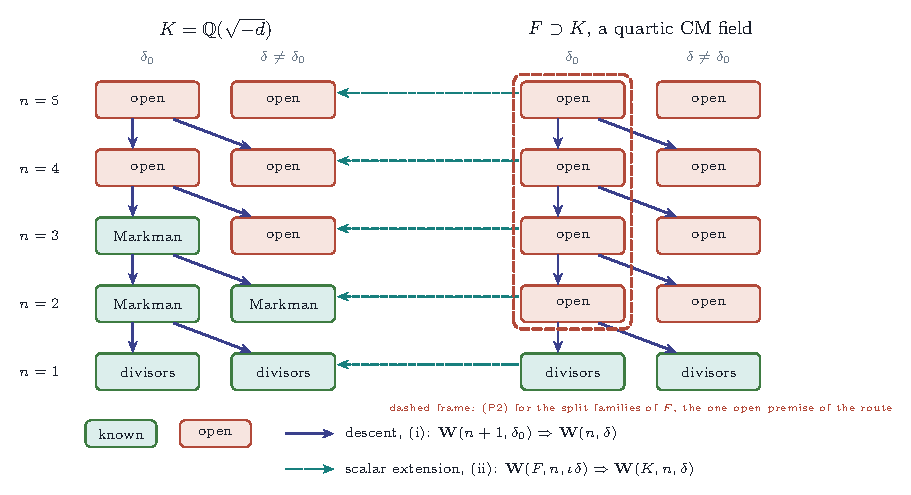
\includegraphics[width=0.94\textwidth]{fig_descent}
\caption{The Weil families of an imaginary quadratic field $K$ and of a
quartic CM field $F\supset K$, one cell for each $n$ and each kind of
discriminant, grass where the Weil classes are proved algebraic
(divisor classes at $n=1$; Markman \cite{Mar25a,Mar25b} at $n=2$ and at
$n=3$, $\delta=\delta_{0}$) and clay where they rest on the open
propagation statement. The indigo arrows
are the descent of \Cref{prop:descent}(i), from the trivial discriminant in
dimension $n+1$ to every discriminant in dimension $n$; the dashed teal
arrows are the scalar extension of \Cref{prop:descent}(ii). The dashed frame
is the propagation statement for the split families of the field of higher
degree, which by \Cref{thm:closure}(ii) is the only form of (P2) that any
minimal route to the conjecture uses: every clay cell of the left panel lies
below it.}
\label{fig:descent}
\end{figure}

\noindent
The list is as follows.

\begin{enumerate}[label=\textup{(C\arabic*)},leftmargin=3.0em,itemsep=4pt]
\item \emph{One secant object on one fourfold.} There should exist a
  principally polarised abelian fourfold $(X,\Theta)$ and a perfect complex
  $\cF$ on it with $\ch(\cF)=u_{\Theta}+3v_{\Theta}$ satisfying
  \cite[(19)]{paperII}. By \cite[Theorem~4.56]{paperII} and \cite[Corollary~4.57]{paperII}
  the transform $\Phi(\cF\boxtimes\cF)$ would then satisfy the weakened
  criterion, and by \cite[Proposition~4.52]{paperII} the three conditions of Markman's
  strategy that concern only the Chern character hold at the point $(1,3)$
  for any such $\cF$, since they depend on $\ch(\cF)$ alone. Turning this
  into algebraicity needs one further input. The weakened criterion enters
  in place of the hypothesis Markman verifies, and the survival of the
  semiregularity theorem under the substitution is exactly
  \cite[Question 11.4]{Mar25b}. So (C1) is a demand on a construction, and an affirmative answer to
  that question is a separate prerequisite standing beside it;
  \Cref{thm:closure} places both. What this paper contributes is the exact
  form of the demand. The local part of the criterion is a condition on depth
  and nothing else: if the support is Cohen--Macaulay there is no local
  obstruction at any point (\cite[Theorem~4.75]{paperII}); if it is not, the local
  $\Ext^{2}$ is nonzero at the bad points, and where two smooth branches of
  codimension two meet transversally the criterion fails outright
  (\cite[Theorem~4.61]{paperII}, \cite[Corollary~4.63]{paperII},
  \cite[Corollary~4.77]{paperII}). The candidate of
  \cite[Section 12]{Mar25b} is of the second kind, and it cannot be moved to
  the first: separating the branches is what would restore the depth, and
  \cite[Remark~4.78]{paperII} shows that doing so moves the Chern character
  off the secant plane. What is needed is therefore a support without such
  points. For a Cohen--Macaulay support the identity \cite[(19)]{paperII}
  is the single vanishing of the image of $A_{\theta}A_{\theta'}$ in
  $H^{1}(Z,\cE xt^{1}(\cI_{Z},\cI_{Z}))$, and the sheaf must in addition
  extend to first order along the polarised deformations
  (\cite[Theorem~4.56(iii)]{paperII}). Such a support has one of two
  shapes (\cite[Corollary~4.94]{paperII}): a smooth one, where the invariants are forced
  outright and $d\le b^{2}$ for the twist $b\Theta$, so $d\le9$ for the twist
  $3\Theta$ of \cite[Setup~4.51]{paperII} (\cite[Theorem~4.67]{paperII},
  \cite[Corollary~4.68]{paperII}), and a singular one. In neither may the
  Hilbert--Burch resolution split into powers of $\Theta$ or into simple
  semi-homogeneous bundles (\cite[Theorem~4.89]{paperII}, \cite[Theorem~4.92]{paperII}), and
  no complete intersection occurs (\cite[Theorem~4.81]{paperII}).
\item \emph{The same for every $n$ and every discriminant.} A positive answer
  to (C1) reaches one triple, and the discriminant of that triple is the
  trivial one, because the object lives on $X\times\widehat X$ and every split
  member has trivial discriminant by \cite[Proposition~15.19(ii)]{paperI}. The other
  triples are reached through \Cref{prop:descent}: a positive answer in
  infinitely many dimensions gives $\mathbf{W}(K,n,\delta)$ for every $n$ and
  every $\delta$, so only uniformity in $n$ is asked for, and (C1) at $n=4$,
  with Question~11.4, already gives every sixfold. No answer of this kind
  reaches the CM fields of degree at least four. What this paper
  contributes: three of the four ingredients of \cite[Question~13.7]{paperI} are supplied
  for every $n$ and every $K$ (\cite[Theorem~14.15]{paperI}), including the
  existence of the secant sheaves themselves (\cite[Theorem~14.13]{paperI}); the
  fourth is isolated exactly (\cite[Remark~14.16]{paperI}).
\item \emph{CM fields of degree larger than two.} For a CM field $F$ of
  degree $2m>2$ acting on an abelian variety, the Weil classes span a space of
  dimension $2m$, and the secant framework of \cite[Section~14]{paperI}, which
  is built on a plane meeting the spinor variety in a conjugate pair, does not
  apply to them as it stands. Markman has extended it to these fields
  \cite{Mar25c}: for an abelian variety $X$ with real multiplication by the
  totally real subfield $F_{0}$ of $F$, a polarisation
  $\Theta\in\bigwedge^{2}_{F_{0}}H^{1}(X,\QQ)$ and $q\in F_{0}$ with
  $F=F_{0}(\sqrt{-q})$, he makes $F$ act on $X\times\widehat{X}$ with split
  Weil type, replaces the plane by a rational subspace $B$ of dimension
  $2^{[F_{0}:\QQ]}$ of the half-spin representation that is secant to the
  spinor variety, and shows that for sheaves $F_{1},F_{2}$ on $X$ with
  characters in $B$ the class $\kappa(E)=\ch(E)\exp(-c_{1}(E)/\rk E)$ of
  $E=\Phi(F_{1}\boxtimes F_{2}^{\vee})$ stays of Hodge type on every member
  of the family, and that where it stays algebraic all Weil classes are
  algebraic \cite[Theorem~1.1.2, Proposition~10.2.1]{Mar25c}. He exhibits
  such a pair meeting his non-degeneracy criterion when $F$ is biquadratic
  and $X$ is the Jacobian of a curve of genus four with real multiplication
  by $F_{0}$ and an automorphism acting through a unit of norm one
  \cite[Example~11.2.7, Lemma~11.2.8]{Mar25c}. That $\kappa(E)$ stays
  algebraic would follow from a semiregularity property of $E$, which is not
  addressed there \cite[Question~11.2.2]{Mar25c}; for the pair of that
  example the weaker property asked in the question fails at the points of
  the glued curves (\cite[Corollary~5.30]{paperII}). No result of this paper
  depends on a theorem of \cite{Mar25c}; \cite[Section~5.2]{paperII} and
  \cite[Section~5.3]{paperII} use its construction as their setting. What this paper
  contributes: everything except the propagation. By \cite[Section~17]{paperI}
  each such family has a connected period domain, a flat space of Weil
  classes, a dense set of rational orbits, a base point at a CM member where
  the classes are written as polynomials in divisor classes
  (\cite[Theorem~17.5]{paperI}), and the two propagation criteria
  (\cite[Theorem~17.7]{paperI}); so the higher CM fields are the same
  propagation problem as the quadratic ones, and not a separate entry. For a
  quartic field at $n=2$, the smallest case of higher degree,
  \cite[Section~5.2]{paperII}
  determines how far divisor classes, scalar extension and correspondences
  reach, and computes the number that the polarised criterion asks of one
  complex. For a sextic field, \cite[Section~5.3]{paperII} shows that the dimension
  count, which excludes a minimal Orlov product over a quartic field, does not
  exclude one over a sextic field, and gives the profile such an object would
  have. \cite[Appendix~C]{paperI} places the imaginary quadratic case inside Albert's
  classification.
\item \emph{The non-split sixfolds.} $\mathbf{W}(K,3,\delta)$ for
  $\delta\ne\delta_{0}$; the case $\delta=\delta_{0}$ is Markman's
  \cite{Mar25a}. By \Cref{prop:descent}(i) it would follow from
  $\mathbf{W}(K,4,\delta_{0})$, and by \Cref{prop:descent}(ii) from
  $\mathbf{W}(K(\sqrt2),3,\iota(\delta))$. What this paper contributes: a base
  point in every family, at a member with quaternionic multiplication
  (\cite[Theorem~15.27]{paperI}); the locus of such members is a Lagrangian
  Grassmannian of codimension $n(n-1)/2$ (\cite[Proposition~15.32]{paperI}), and
  the rest of the family can be reached from it only by propagation.
\item \emph{Exceptional classes that are not of Weil type.} On an abelian
  variety the Hodge ring can contain exceptional classes that the Weil
  construction does not produce. Through dimension five it does not
  \cite{MZ99}, and in dimension eight it does: the self-product of an abelian
  fourfold of Mumford type carries two Hodge classes that are neither
  products of divisor classes nor Weil classes of any quotient
  (\Cref{prop:mumfordproduct}). So the Hodge conjecture for abelian varieties
  does not reduce to Weil classes, and the statement needed is the
  algebraicity of these classes themselves. What this paper contributes: the
  example, made exact, and the forms of their algebraicity studied in
  \Cref{sec:beyond}.
\item \emph{Varieties that are not abelian.} A reduction of the Hodge
  conjecture for arbitrary smooth projective varieties to abelian varieties
  cannot be of Hodge-theoretic kind: the $H^{3}$ of a very
  general quintic threefold lies outside the tensor category generated by the
  cohomology of abelian varieties (\Cref{prop:noabeliantype}), so its Hodge
  structure cannot be realised inside that of an abelian variety by any
  correspondence. \cite[Theorem~10.3]{paperI} and \cite[Theorem~10.8]{paperI} close the
  two routes through hyperplane sections that would be the natural candidates.
  What this paper contributes: those three obstructions and, on the positive
  side, special cases only (\Cref{prop:mumfordfivefold},
  \Cref{rem:f3primefrontier}). Nor is this entry the complement of the others. The varieties
  that are not abelian include $A\times\PP^{1}$ for every abelian variety
  $A$, and the
  conjecture for $A\times\PP^{1}$ gives it for $A$, so the conjecture for
  the varieties that are not abelian is the whole conjecture
  (\Cref{prop:f3ishc}).
\end{enumerate}

\subsection{Implications from the literature}\label{ssec:bullseye}

The theorems of this paper are not the only implications that end in the
conjecture. The literature supplies others, and a frontier drawn without
them overstates what is needed. This subsection proves those implications, or
quotes them where they are theorems of the literature, so that
\Cref{ssec:closure} runs over both. Nothing in it is new
except the assembly, but the assembly changes the answer.

\begin{definition}[Three statements about all varieties]\label{def:lmv}
Here a variety is smooth, projective and defined over $\CC$, except the base
$S$ in \textup{(V)}.
\begin{enumerate}[leftmargin=3.0em,itemsep=3pt]
\item[\textup{(L)}] $B(X)$ holds for every variety $X$ (\cite[Definition~10.6]{paperI}).
\item[\textup{(M)}] Every Hodge class on every variety $X$ is
  \emph{motivated} in the sense of Andr\'e \cite[\S2.1]{And96b}: it equals
  $\mathrm{pr}_{*}(\alpha\cup{*}\beta)$ for some variety $Y$, algebraic
  classes $\alpha,\beta$ on $X\times Y$, the projection
  $\mathrm{pr}\colon X\times Y\to X$, and the Lefschetz involution ${*}$ of
  $H^{*}(X\times Y,\QQ)$ with respect to some ample class.
\item[\textup{(V)}] For every smooth connected complex variety $S$, every
  smooth projective morphism $f\colon\cX\to S$ and every global section $\xi$
  of $R^{2p}f_{*}\QQ$ over $S^{\mathrm{an}}$: if $\xi_{s}$ is algebraic at one
  point $s\in S$, then $\xi_{t}$ is algebraic at every point $t\in S$.
\end{enumerate}
The Lefschetz involution of a variety $Z$ of dimension $e$ with ample class
$L$ sends $L^{r}x$, for $x$ primitive of degree $j$ and $0\le r\le e-j$, to
$\pm L^{e-j-r}x$, with a sign that depends only on $j$ \cite{And96b}; the
sign plays no role below.
\end{definition}

The statement (V) is the variational Hodge conjecture for algebraic classes;
it asks nothing about Hodge classes, only that algebraicity, once present,
survives deformation.

\begin{lemma}[Kleiman]\label{lem:lefinvolution}
Let $Z$ be a variety of dimension $e$ with ample class $L$, and suppose that
$B(Z)$ holds. Then the K\"unneth projectors $\pi_{k}$ of $H^{*}(Z,\QQ)$, the
projectors onto the summands $L^{r}P^{j}$ of the Lefschetz decomposition, and
the Lefschetz involution ${*}$ are all induced by algebraic cycles on
$Z\times Z$.
\end{lemma}

\begin{proof}
Operators induced by algebraic cycles on $Z\times Z$ are closed under sums
and rational multiples, and under composition, because the composite of two
algebraic correspondences is again algebraic \cite{Kle68}. The operator $L$
is induced by the image of a divisor of class $L$ under the diagonal, and $\Lambda$ by $B(Z)$. With
$[L,\Lambda]=H$ and $H$ acting on $H^{k}$ by $k-e$ (the proof of
\cite[Lemma~10.7]{paperI}), $H=L\Lambda-\Lambda L$ is induced by an algebraic cycle,
and since the numbers $k-e$ for $0\le k\le 2e$ are distinct,
\[
  \pi_{k}=\prod_{i\ne k}\frac{H-(i-e)}{k-i}
\]
is as well. Put $\Omega=H^{2}+2H+4\Lambda L$. For $x$ primitive of degree
$j$ put $m=e-j\ge0$. Then $\Lambda x=0$ and $Hx=-mx$, and the relation
\begin{equation}\label{eq:lambdapower}
  \Lambda L^{s}x=s(m-s+1)\,L^{s-1}x\qquad(s\ge1)
\end{equation}
follows by induction from $\Lambda L=L\Lambda-H$: the case $s=1$ is
\cite[Lemma~10.7]{paperI}, and
$\Lambda L^{s}x=L\Lambda L^{s-1}x-HL^{s-1}x
=\bigl((s-1)(m-s+2)-(2s-2-m)\bigr)L^{s-1}x=s(m-s+1)L^{s-1}x$.
So $\Omega x=(m^{2}-2m+4m)x=m(m+2)x$, and $\Omega$ commutes with $L$, since
$[L,H]=-2L$ and $[L,\Lambda L]=HL$ give $[L,\Omega]=-2(LH+HL)-4L+4HL=0$;
hence $\Omega$ acts on $L^{r}P^{j}$ by $m(m+2)$. Inside $H^{k}$ the summands
are $L^{r}P^{k-2r}$, with $m=e-k+2r$, and $m\mapsto m(m+2)$ is injective on
$m\ge0$, so Lagrange interpolation in $\Omega$ composed with $\pi_{k}$ gives
the projector $p_{k,r}$ onto $L^{r}P^{k-2r}$ as an algebraic operator.
Finally let $x\in P^{j}$ and $0\le r\le m$. If $2r\le m$, then
$L^{m-2r}(L^{r}x)=L^{m-r}x$. If $2r>m$, put $t=2r-m$, so $1\le t\le r$;
by \eqref{eq:lambdapower},
\[
  \Lambda^{t}L^{r}x=\prod_{i=0}^{t-1}(r-i)(m-r+i+1)\;L^{m-r}x,
\]
and every factor is at least $1$, because $r-i\ge r-t+1\ge1$ and
$m-r+i+1\ge m-r+1\ge1$. So on $L^{r}P^{j}$ the involution is $\pm L^{m-2r}$
or a nonzero rational multiple of $\Lambda^{2r-m}$, and
${*}=\sum_{k,r}c_{k,r}T_{k,r}\,p_{k,r}$ with rational $c_{k,r}$ and
$T_{k,r}$ a power of $L$ or of $\Lambda$. Every term is algebraic.
\end{proof}

\begin{proposition}[The conjecture is (L) and (M)]\label{prop:lefmot}
The Hodge conjecture for every variety is equivalent to \textup{(L)} and
\textup{(M)} together.
\end{proposition}

\begin{proof}
Assume the conjecture. Then \textup{(L)} holds by \cite[Theorem~12.2]{paperI}. An
algebraic class $\xi$ on $X$ of dimension $d$ is motivated: take $Y$ a point,
$\alpha=\xi$, and $\beta=\varepsilon h^{d}$ with $h$ the ample class and
$\varepsilon=\pm1$ the sign for which ${*}(h^{d})=\varepsilon$, which exists
because the unit $1\in H^{0}$ is primitive of degree $0$; then
$\alpha\cup{*}\beta=\xi$. Every Hodge class is algebraic, so \textup{(M)}
holds.

Conversely assume \textup{(L)} and \textup{(M)}, and let $\xi$ be a Hodge
class on $X$. By \textup{(M)}, $\xi=\mathrm{pr}_{*}(\alpha\cup{*}\beta)$ with
$\alpha,\beta$ algebraic on $X\times Y$. By \textup{(L)}, $B(X\times Y)$
holds, so ${*}$ is induced by an algebraic cycle
(\Cref{lem:lefinvolution}); hence ${*}\beta$, the product
$\alpha\cup{*}\beta$ and its push-forward $\xi$ are algebraic. This is
Andr\'e's observation that motivated classes are algebraic as soon as the
Lefschetz involutions are \cite[\S2.1]{And96b}.
\end{proof}

\begin{proposition}[Two sources of (V)]\label{prop:lefvhc}
The Hodge conjecture implies \textup{(V)}, and so does \textup{(L)}.
\end{proposition}

\begin{proof}
Let $f\colon\cX\to S$, $\xi$ and $s$ be as in \textup{(V)}, with $\xi_{s}$
algebraic. As $S$ is smooth and connected it is irreducible, so two affine
open subsets meet, and it suffices to treat $S$ affine, joining $s$ to an
arbitrary $t$ through a point of the intersection of an affine neighbourhood
of each. Then $\cX$ is quasi-projective and, by resolution of singularities,
has a smooth projective compactification $\overline{\cX}$.

Assume the conjecture. Write $n=2p$ and
$\rho\colon H^{n}(\overline{\cX},\QQ)\to H^{0}(S^{\mathrm{an}},R^{n}f_{*}\QQ)$
for restriction; it is surjective by the theorem of the fixed part
\cite[4.1.1(ii)]{Del71}. For $t\in S$ the restriction
$r_{t}\colon H^{n}(\overline{\cX},\QQ)\to H^{n}(\cX_{t},\QQ)$ is $\rho$
followed by evaluation at $t$, and evaluation is injective because $S$ is
connected; so $K=\ker r_{t}=\ker\rho$ does not depend on $t$. It is a
sub-Hodge structure, and the Hodge structure $H^{n}(\overline{\cX},\QQ)$ is
polarisable, hence semisimple, so $H^{n}(\overline{\cX},\QQ)=K\oplus K'$
with $K'$ a sub-Hodge structure. Choose $\eta\in K'$ with $\rho(\eta)=\xi$.
Then $r_{s}|_{K'}$ is an injective morphism of Hodge structures and
$r_{s}(\eta)=\xi_{s}$ is of type $(p,p)$, so every component of $\eta$ of
type other than $(p,p)$ maps to zero and is zero: $\eta$ is a Hodge class.
So $\xi_{t}=r_{t}(\eta)$ is a Hodge class on $\cX_{t}$ for every $t$, and
algebraic by the conjecture.

Assume \textup{(L)}. The algebraic class $\xi_{s}$ is motivated (proof of
\Cref{prop:lefmot}), so $\xi_{t}$ is motivated for every $t$ by Andr\'e's
deformation theorem \cite[Th\'eor\`eme~0.5]{And96b}, and a motivated class is
algebraic under \textup{(L)} (proof of \Cref{prop:lefmot}).
\end{proof}

\begin{theorem}[Deligne, Andr\'e; Abdulali, Andr\'e]\label{thm:vhcab}
\textup{(V)} implies the Hodge conjecture for every abelian variety, and so
does \textup{(L)}.
\end{theorem}

\begin{proof}
Milne calls a class \emph{accessible} if it lies in the least family of
rational classes that contains the classes of algebraic cycles, is stable
under pull-back by morphisms of varieties, and contains $t_{t}$ for every $t$
whenever $(t_{s})_{s\in S}$ is a global section of $R^{r}f_{*}\QQ$ for a
smooth projective family over a smooth connected base and contains $t_{s}$
for one $s$; and he proves, following Deligne and Andr\'e, that every Hodge
class on an abelian variety is accessible \cite[\S5.1, Theorem~3]{Mil20}.
The algebraic classes contain the classes of algebraic cycles and are stable
under pull-back, and under \textup{(V)} they have the third property. So they
contain every accessible class, hence every Hodge class on an abelian
variety; this is \cite[Remark~2]{Mil20}. The statement for \textup{(L)}
follows by \Cref{prop:lefvhc}, and is the theorem of Abdulali and Andr\'e in
the form of \cite[Theorem~4]{Mil20}.
\end{proof}

\begin{remark}[The three in the literature]\label{rem:lmvknown}
$B(X)$ is known for curves, where it is immediate,
and for abelian varieties \cite[\S2]{Kle68}, and \Cref{cor:mumfordlefschetz}
below adds the total space of every Mumford family. \textup{(M)} holds for the Hodge
classes on abelian varieties \cite[Th\'eor\`eme~0.6.2]{And96b}.
\textup{(V)} holds in degree $2$, where by the argument of
\Cref{prop:lefvhc} the class $\xi_{t}$ is a Hodge class and the Lefschetz
theorem on $(1,1)$ classes applies; the one general mechanism for it in
higher degree is the semiregularity theorem \cite{Blo72,BF03,Pri24}, which is the
mechanism of \cite[Theorem~2.3]{paperII}. \Cref{thm:vhcab} says what is at
stake for this paper: the single statement \textup{(V)}, which the conjecture
itself implies, gives the Weil classes of every CM field and the classes
beyond the Weil lines at once, by a route that uses none of the theorems
proved here.
\end{remark}

\subsection{The Lefschetz standard conjecture for abelian schemes over curves}
\label{ssec:newlefschetz}

The statement $B(X)$ is known for abelian varieties $X$. This subsection
proves it for the total space
of an abelian scheme over a curve whose invariant cycles are algebraic, and
so for the total space of every Mumford family. The proof assembles the
operator $\Lambda$ from a relative part, which is a Pontryagin product and is
algebraic on every abelian scheme, and a part along the base, which is
algebraic exactly when the invariant cycles are.

\begin{proposition}[$\Lambda$ as a Pontryagin product]
\label{prop:pontryaginlambda}
Let $A$ be an abelian variety of dimension $g$, $\ell\in H^{2}(A,\QQ)$ the
class of an ample line bundle, $D=\int_{A}\ell^{g}/g!$ and
$\gamma=\ell^{g-1}/(g-1)!$. Let $\mu\colon A\times A\to A$ be the addition
and $x\star y=\mu_{*}(p_{1}^{*}x\cup p_{2}^{*}y)$ the Pontryagin product.
Then the operator $\Lambda$ of \cite[Definition~10.6]{paperI} for the class $\ell$ is
\[
  \Lambda(x)=D^{-1}\,x\star\gamma .
\]
In particular $\Lambda$ is induced by the algebraic cycle
$D^{-1}(p_{1},\mu)_{*}(p_{2}^{*}Z)$ on $A\times A$, for any cycle $Z$ of
class $\gamma$.
\end{proposition}

\begin{proof}
Put $V=H_{1}(A,\QQ)$, so that $H^{*}(A,\QQ)=\bigwedge^{*}V^{\vee}$ under cup
product and $H_{*}(A,\QQ)=\bigwedge^{*}V$ under the Pontryagin product of
homology, and let $\mathrm{PD}(x)=x\cap[A]$. Cap product makes
$H_{*}$ a module over $H^{*}$, and for a torus it is contraction; so
$\mathrm{PD}(\ell\cup x)=\ell\cap\mathrm{PD}(x)$ is the contraction
$\iota_{\ell}$ applied to $\mathrm{PD}(x)$. Poincar\'e duality commutes
with $\mu_{*}$ and carries $p_{1}^{*}x\cup p_{2}^{*}y$ to the cross product
of $\mathrm{PD}(x)$ and $\mathrm{PD}(y)$, without sign when $y$ has even
degree, so $\mathrm{PD}(x\star\gamma)=\mathrm{PD}(x)\cdot\beta$ with
$\beta=\mathrm{PD}(\gamma)\in\bigwedge^{2}V$.

Choose a basis $x_{1},y_{1},\dots,x_{g},y_{g}$ of $V^{\vee}$ with
$\ell=\sum_{i}d_{i}\,x_{i}\wedge y_{i}$, $d_{i}>0$, oriented so that
$\int_{A}x_{1}\wedge y_{1}\wedge\dots\wedge x_{g}\wedge y_{g}=1$; then
$\int_{A}\ell^{g}=g!\,d_{1}\cdots d_{g}$, so $D=d_{1}\cdots d_{g}$. Let
$e_{i},f_{i}$ be the dual basis of $V$. Then
$\gamma=\sum_{j}\bigl(\prod_{i\ne j}d_{i}\bigr)\prod_{i\ne j}x_{i}\wedge y_{i}$
and $\beta=\varepsilon D\sum_{j}d_{j}^{-1}e_{j}\wedge f_{j}$ with
$\varepsilon=\pm1$ independent of $j$, since the permutations of the pairs
preserve the orientation and exchange the terms. The algebra $\bigwedge^{*}V$
is the graded tensor product of the algebras
$\bigwedge^{*}\langle e_{i},f_{i}\rangle$, and $\iota_{\ell}$ and
multiplication by $D^{-1}\beta$ are sums over $i$ of even operators on the
$i$-th factor, namely $d_{i}\,\iota_{x_{i}\wedge y_{i}}$ and
$\varepsilon d_{i}^{-1}e_{i}\wedge f_{i}$. Operators on different factors
commute, and on the $i$-th factor, with basis $1,e_{i},f_{i},e_{i}\wedge
f_{i}$ and $\iota_{x_{i}\wedge y_{i}}(e_{i}\wedge f_{i})=\sigma$ for a sign
$\sigma$ fixed by the convention for contraction, the commutator
$[\iota_{\ell},D^{-1}\beta]$ acts by $\varepsilon\sigma$ on $1$, by $0$ on
$e_{i}$ and $f_{i}$, and by $-\varepsilon\sigma$ on $e_{i}\wedge f_{i}$, that
is by $\varepsilon\sigma(1-k_{i})$ in degree $k_{i}$. Summing over $i$,
$[\iota_{\ell},D^{-1}\beta]=\varepsilon\sigma(g-k)$ on $\bigwedge^{k}V$. As
$\mathrm{PD}$ carries $H^{q}$ to $\bigwedge^{2g-q}V$, the operator
$\Lambda'(x)=D^{-1}x\star\gamma$ satisfies
$[L,\Lambda']=\varepsilon\sigma(q-g)=\varepsilon\sigma H$ on $H^{q}(A)$.

The sign is fixed by one value. For $x$ and $y$ of complementary degrees,
$x\star y\in H^{0}(A)$ is $\int_{A\times A}p_{1}^{*}x\cup p_{2}^{*}y\cup
\mu^{*}[\mathrm{pt}]$, and $\mu^{*}[\mathrm{pt}]$ is the class of the
antidiagonal $\{(a,-a)\}$, so $x\star y=\int_{A}x\cup[-1]^{*}y$; for
$y=\gamma$, of even degree, this is $\int_{A}x\cup\gamma$. Hence
$\Lambda'(\ell)=D^{-1}\int_{A}\ell\cup\gamma=g$, while
$\Lambda(\ell)=\Lambda(L\cdot1)=g$ by \cite[Lemma~10.7]{paperI}. If
$\varepsilon\sigma=-1$, then $-\Lambda'$ would be the operator of
\cite[Definition~10.6]{paperI} and $\Lambda'(\ell)=-g$. So $\varepsilon\sigma=1$, and
$\Lambda'=\Lambda$ by the uniqueness in \cite[Definition~10.6]{paperI}. Finally, the
correspondence $(p_{1},\mu)_{*}(p_{2}^{*}Z)$ acts by
$x\mapsto p_{2*}\bigl(p_{1}^{*}x\cup(p_{1},\mu)_{*}p_{2}^{*}[Z]\bigr)
=\mu_{*}(p_{1}^{*}x\cup p_{2}^{*}\gamma)$, by the projection formula.
\end{proof}

\begin{theorem}[The Lefschetz operator of an abelian scheme over a curve;
cf.\ Tankeev \cite{Tan03}]
\label{thm:lefschetzfamily}
Let $C$ be a smooth projective connected curve and $\pi\colon W\to C$ an
abelian scheme of relative dimension $g$ with $W$ projective. Suppose that
every class in $H^{*}(W_{c},\QQ)$ invariant under the monodromy of
$R^{*}\pi_{*}\QQ$ is the restriction of an algebraic class on $W$. Then there
is an ample class $L_{W}$ on $W$ whose operator $\Lambda$ is induced by an
algebraic cycle on $W\times W$: $B(W)$ holds.
\end{theorem}

\begin{proof}
\emph{Step 1: the decomposition.} Let $[n]\colon W\to W$ be multiplication
by $n$ over $C$. It acts on $R^{q}\pi_{*}\QQ=\bigwedge^{q}R^{1}\pi_{*}\QQ$ by
$n^{q}$. The Leray spectral sequence degenerates \cite[4.1.1(i)]{Del71}, and
$[2]^{*}$ preserves the Leray filtration and acts on its graded pieces
$H^{p}(C,R^{q}\pi_{*}\QQ)$ by $2^{q}$. So $H^{k}(W,\QQ)=\bigoplus_{q}
H^{k}_{(q)}$, where $H^{k}_{(q)}$ is the $2^{q}$-eigenspace of $[2]^{*}$ and
maps isomorphically onto $H^{k-q}(C,R^{q}\pi_{*}\QQ)$; only $k-q\in\{0,1,2\}$
occurs. The projectors
$P_{q}=\prod_{q'\ne q}([2]^{*}-2^{q'})/(2^{q}-2^{q'})$ are induced by
algebraic cycles, polynomials in the graph of $[2]$. As $[2]^{*}$ is a ring
homomorphism, $H_{(q)}\cup H_{(q')}\subset H_{(q+q')}$; as
$\int_{W}[2]^{*}z=2^{2g}\int_{W}z$, the integral vanishes on $H_{(q)}$ for
$q\ne2g$, so Poincar\'e duality pairs $H_{(q)}$ with $H_{(2g-q)}$ only; and
$[2]_{*}=2^{2g}([2]^{*})^{-1}$ acts on $H_{(q)}$ by $2^{2g-q}$.

\emph{Step 2: the ample class.} Let $\cL$ be a relatively ample line bundle,
replaced by $\cL\otimes[-1]^{*}\cL$ so that it is symmetric. Then $[-1]^{*}$
fixes $c_{1}(\cL)$ and acts on $H_{(q)}$ by $(-1)^{q}$, so $c_{1}(\cL)$ has no
component in $H^{2}_{(1)}$, while $H^{2}_{(0)}=H^{2}(C,\QQ)$ is spanned by the
class $f$ of a fibre. So $c_{1}(\cL)=\ell+af$ with $\ell\in H^{2}_{(2)}$
algebraic and $a\in\QQ$. Put $L_{W}=\ell+mf=c_{1}(\cL)+(m-a)f$ with
$m\in\QQ$ so large that $L_{W}$ is a positive rational multiple of the class
of an ample line bundle, which is possible because $\cL$ is relatively ample.
Write $L_{\mathrm{rel}}$ and $L_{C}$ for cup product with $\ell$ and with
$mf$, so that $L_{W}=L_{\mathrm{rel}}+L_{C}$; on
$H^{p}(C,R^{q}\pi_{*}\QQ)$ the first raises $q$ by two and the second raises
$p$ by two.

\emph{Step 3: the relative operator.} Put $\gamma=\ell^{g-1}/(g-1)!$, which is
algebraic and lies in $H_{(2g-2)}$, and $D=\int_{W_{c}}\ell^{g}/g!$. Let
$\mu,\mathrm{pr}_{1},\mathrm{pr}_{2}\colon W\times_{C}W\to W$ be the addition
and the projections, and $T(x)=\mu_{*}(\mathrm{pr}_{1}^{*}x\cup
\mathrm{pr}_{2}^{*}\gamma)$. As in \Cref{prop:pontryaginlambda}, $T$ is
induced by the algebraic cycle $(\mathrm{pr}_{1},\mu)_{*}(\mathrm{pr}_{2}^{*}Z)$
on $W\times W$. Since $\pi\circ\mathrm{pr}_{1}=\pi\circ\mu$, the projection
formula gives $T(x\cup\pi^{*}b)=T(x)\cup\pi^{*}b$, so $T$ commutes with
$L_{C}$. Since $[2]\circ\mu=\mu\circ([2]\times_{C}[2])$,
$[2]_{*}T(x)=\mu_{*}(\mathrm{pr}_{1}^{*}[2]_{*}x\cup\mathrm{pr}_{2}^{*}
[2]_{*}\gamma)$, and for $x\in H_{(q)}$ this is
$2^{2g-q}\,2^{2}\,T(x)$; so $T$ maps $H_{(q)}$ into $H_{(q-2)}$. A relative
correspondence acts on the Leray spectral sequence through the maps it
induces on the local systems, so on $H^{p}(C,R^{q}\pi_{*}\QQ)$ the operator
$T$ is $H^{p}(C,T_{\bullet})$, with $T_{c}$ the Pontryagin product with
$\gamma|_{W_{c}}$ on the fibre. By \Cref{prop:pontryaginlambda}, $D^{-1}T_{c}$
is the operator $\Lambda$ of the fibre, so $\Lambda_{\mathrm{rel}}=D^{-1}T$
satisfies $[L_{\mathrm{rel}},\Lambda_{\mathrm{rel}}]=H_{\mathrm{rel}}$, where
$H_{\mathrm{rel}}$ acts on $H_{(q)}$ by $q-g$.

\emph{Step 4: the invariant classes.} Restriction maps $H^{q}(W,\QQ)$ onto the
monodromy invariants $I_{q}\subset H^{q}(W_{c},\QQ)$ \cite[4.1.1(ii)]{Del71},
and it kills $H^{q}_{(q')}$ for $q'<q$, which lies in positive Leray degree;
so it maps $H^{q}_{(q)}$ isomorphically onto $I_{q}$. Every element of
$H^{q}_{(q)}$ is algebraic: if $v\in I_{q}$ is the restriction of an algebraic
class $z$, then $P_{q}z$ is algebraic, lies in $H^{q}_{(q)}$ and restricts to
$v$. The subspace $I_{q}$ is a sub-Hodge structure, as the image of a
morphism of Hodge structures, and it is stable under cup product with
$\ell_{c}$ and under the operator $\Lambda$ of the fibre, which are the
restrictions of $L_{\mathrm{rel}}$ and $\Lambda_{\mathrm{rel}}$. The
polarisation of $H^{q}(W_{c},\QQ)$ attached to $\ell_{c}$ has the form
$(v,w)\mapsto\int_{W_{c}}v\cup S(w)$, with $S$ a polynomial in cup product
with $\ell_{c}$, the operator $\Lambda$ and the projectors of the fibre, and
its restriction to the sub-Hodge structure $I_{q}$ is again a polarisation
\cite{Voi02}. Since $S(I_{q})\subset I_{2g-q}$, the pairing
$I_{q}\times I_{2g-q}\to\QQ$ is nondegenerate.

\emph{Step 5: the operator along the base.} For $y\in H^{q}_{(q)}$ and
$w\in H^{2g-q}_{(2g-q)}$ one has $\int_{W}(y\cup f)\cup w=\int_{W_{c}}
y|_{W_{c}}\cup w|_{W_{c}}$. By Step 4 and Step 1 this shows that
$L_{C}\colon H^{q}_{(q)}\to H^{q+2}_{(q)}$ is injective, and it is onto
because $\dim H^{q+2}_{(q)}=\dim H^{2g-q}_{(2g-q)}=\dim I_{2g-q}=\dim I_{q}$,
by Poincar\'e duality on $W$ and on the invariants. Choose bases $(a_{j})$ of
$H^{q}_{(q)}$ and $(b_{k})$ of $H^{2g-q}_{(2g-q)}$, all algebraic by Step 4,
let $M_{jk}=\int_{W}a_{j}\cup mf\cup b_{k}$, which is invertible, and put
\[
  \Lambda_{C}(x)=\sum_{j,k}(M^{-1})_{kj}\Bigl(\int_{W}x\cup b_{k}\Bigr)a_{j}
  \qquad(x\in H^{q+2}(W,\QQ)),
\]
for every $q$. It is induced by the algebraic cycle
$\sum_{j,k}(M^{-1})_{kj}\,b_{k}\times a_{j}$. By Step 1, $\int_{W}x\cup b_{k}$
vanishes for $x\in H^{q+2}_{(q')}$ with $q'\ne q$, so $\Lambda_{C}$ is zero
on $H^{p}(C,R^{q}\pi_{*}\QQ)$ for $p\ne2$, and $\Lambda_{C}(L_{C}a_{i})=a_{i}$.
Hence $[L_{C},\Lambda_{C}]$ is $-1$ on $H_{(q)}^{q}$, $0$ on
$H_{(q)}^{q+1}$ and $+1$ on $H_{(q)}^{q+2}$: it is the operator $H_{C}$ that
acts on $H^{p}(C,R^{q}\pi_{*}\QQ)$ by $p-1$.

\emph{Step 6: the cross relations and the conclusion.} $[L_{C},
\Lambda_{\mathrm{rel}}]=0$ by Step 3. Both $L_{\mathrm{rel}}\Lambda_{C}$ and
$\Lambda_{C}L_{\mathrm{rel}}$ vanish off the summands with $p=2$, and on
$L_{C}y$ with $y\in H^{q}_{(q)}$ both give $\ell\cup y$, because
$\ell\cup y\in H^{q+2}_{(q+2)}$ and $L_{C}$ commutes with $L_{\mathrm{rel}}$;
so $[L_{\mathrm{rel}},\Lambda_{C}]=0$. Put
$\Lambda=\Lambda_{\mathrm{rel}}+\Lambda_{C}$, of degree $-2$. Then
\[
  [L_{W},\Lambda]=[L_{\mathrm{rel}},\Lambda_{\mathrm{rel}}]+[L_{C},\Lambda_{C}]
  =H_{\mathrm{rel}}+H_{C},
\]
which acts on $H^{p}(C,R^{q}\pi_{*}\QQ)\subset H^{p+q}(W)$ by
$(q-g)+(p-1)=(p+q)-\dim W$. So $\Lambda$ is the operator of \cite[Definition~10.6]{paperI}
for $L_{W}$, by its uniqueness, and it is induced by an algebraic cycle by
Steps 3 and 5.
\end{proof}

\Cref{fig:lefschetzgrid} draws the summands of the proof in relative
dimension four.

\begin{corollary}[Mumford families]\label{cor:mumfordlefschetz}
Let $\pi\colon W\to C$ be a non-isotrivial abelian scheme of relative dimension
four over a smooth projective connected curve, $W$ projective, whose very
general fibre $X$ is a fourfold as in \Cref{prop:mumfordproduct}, with Hodge
group the group $G$ of Mumford's construction \cite{Mum69}, the restriction of
scalars from a totally real cubic field $F$ of the norm one group of a
quaternion algebra over $F$. Then $B(W)$ holds. Such families exist, over the
compact Shimura curves of \cite{Mum69}.
\end{corollary}

\begin{proof}
By Andr\'e's theorem \cite[Theorem~1]{And92} the connected monodromy group is
a normal subgroup of the derived Mumford--Tate group of $X$, which is $G$. It
is not trivial, because the family is not isotrivial, and $G$ is $\QQ$-simple,
since over $\overline{\QQ}$ its three factors are indexed by the embeddings of
$F$ and permuted transitively by the Galois group; so it is $G$. The
monodromy invariants in $H^{*}(X,\QQ)$ are therefore contained in the
invariants of $G$, which are the Hodge classes of $X$, and these are the
powers of the polarisation by \Cref{prop:mumfordproduct}(i). The powers
of $\ell$ restrict to the powers of the polarisation, so every invariant class
is the restriction of an algebraic class, and \Cref{thm:lefschetzfamily}
applies.
\end{proof}

\begin{figure}[tbp]
\centering
  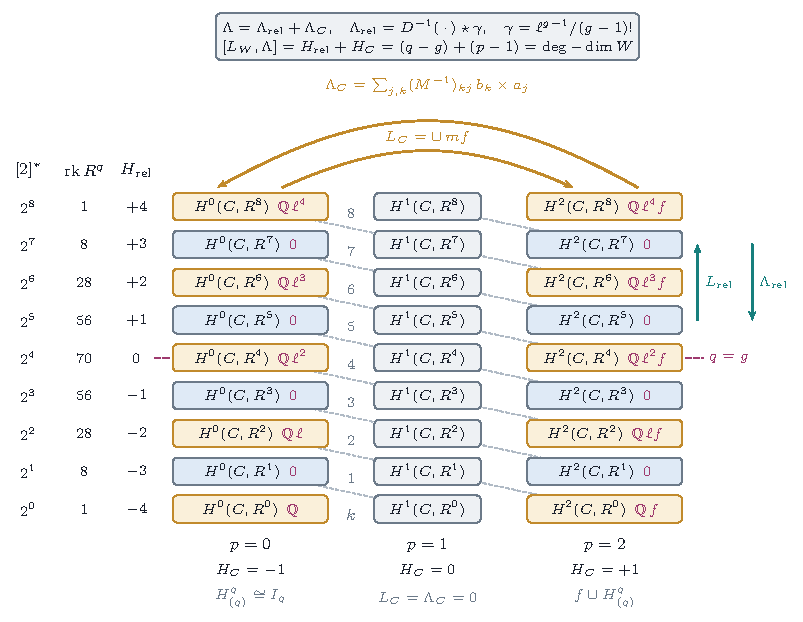
\includegraphics[width=0.86\textwidth]{fig_lefschetzgrid}
\caption{The proof of \Cref{thm:lefschetzfamily} for relative dimension
four. The boxes are the summands $H^{p}(C,R^{q}\pi_{*}\QQ)$ of $H^{*}(W,\QQ)$,
split off by the eigenvalue $2^{q}$ of $[2]^{*}$ shown on the left; the dotted
diagonals join the summands of one $H^{k}(W,\QQ)$, $k=p+q$, and the dashed
magenta line is the axis $q=g$ of hard Lefschetz on the fibres. The relative
operators $L_{\mathrm{rel}}$ and $\Lambda_{\mathrm{rel}}$, in teal, move
within a column; $\Lambda_{\mathrm{rel}}$ is a Pontryagin product with an
algebraic class on every abelian scheme (\Cref{prop:pontryaginlambda}). The
base operators $L_{C}$ and $\Lambda_{C}$, in ochre, move along a row between
the outer columns and kill the middle one; $\Lambda_{C}$ is the displayed
cycle built from bases $(a_{j})$, $(b_{k})$ of the invariant summands, and is
algebraic exactly when the invariant cycles are. Below each column is the
weight of $H=[L_{W},\Lambda]$ on it, and the panel at the top is Step 6 of the
proof. The ochre boxes carry the invariant cycles and their images under
$L_{C}$; for a Mumford family they are the lines listed in magenta on the
right, spanned by $\ell^{i}f$ (and by $\ell^{i}$ in the left column), and the
other boxes of the outer columns are zero (\Cref{cor:mumfordlefschetz}).}
\label{fig:lefschetzgrid}
\end{figure}

\begin{remark}[Scope of the argument]\label{rem:newlefschetzscope}
The total space $W$ is a fivefold fibred in abelian fourfolds whose Hodge
groups are not defined by endomorphisms; it is not a product and not an
abelian variety. For abelian schemes over curves the mechanism of
\Cref{thm:lefschetzfamily} goes back to Tankeev \cite{Tan03}, who proves $B$
for the total space when certain canonically defined Hodge cycles are
algebraic; the argument here does not use his hypotheses, and we make no
claim of priority for \Cref{cor:mumfordlefschetz}. The difficulty lies in the hypothesis of
\Cref{thm:lefschetzfamily}.
Applied to the fibre square $W\times_{C}W\to C$ the theorem gives
$B(W\times_{C}W)$ as soon as every invariant class of $X\times X$ is the
restriction of an algebraic class on $W\times_{C}W$; the invariant classes
include the two exceptional classes of \Cref{prop:mumfordproduct}, so this
is the smallest case of (F2) in a global form. \Cref{thm:lefschetzfamily} does not bear on (P2), on the Kuga--Satake
class of \Cref{thm:mumfordks}, or on \textup{(L)} for varieties that are not
fibred in abelian varieties over a curve.
\end{remark}

\begin{proposition}[Powers of a Weil variety; cf.\ \cite{Mil22}]\label{prop:powers}
Let $X$ be of $(K,-1,n)$-Weil type with $n\ge2$ and $\Hg(X)=\SU(V,H)$. For
every $k\ge1$ the $\QQ$-algebra $\Hdg^{*}(X^{k})$ is generated by the divisor
classes of $X^{k}$ and the pull-backs $f_{a}^{*}\omega$ of the Weil classes
$\omega$ of $X$ along the homomorphisms $f_{a}=\sum_{j}a_{j}\,pr_{j}\colon
X^{k}\to X$, $a\in\ZZ^{k}$. Consequently, if the Weil classes of $X$ are
algebraic, the Hodge conjecture holds for every power of $X$. By
\cite{Mar25a} this is so for every such $X$ with $n=2$, and with $n=3$ and
trivial discriminant.
\end{proposition}

\begin{proof}
Write $H^{1}(X,\CC)=V_{+}\oplus V_{-}$ for the eigenspaces of $K$ and
$W=V_{+}$. The polarisation makes $V_{+}$ and $V_{-}$ isotropic and pairs them
perfectly, so $V_{-}=W^{\vee}$, and restriction to $V_{+}$ identifies
$\SU(V,H)_{\CC}$ with $\SL(W)$. As $\Hg(X^{k})$ is $\Hg(X)$ acting diagonally
on $H^{1}(X^{k},\CC)=(W\otimes U)\oplus(W^{\vee}\otimes U)$, $U=\CC^{k}$, the
Hodge classes of $X^{k}$, tensored with $\CC$, are the $\SL(W)$-invariants in
$\bigwedge^{*}\bigl((W\otimes U)\oplus(W^{\vee}\otimes U)\bigr)$. That algebra
is an $\SL(W)$-equivariant quotient of a tensor algebra, with an equivariant
section given by antisymmetrisation, so Weyl's first fundamental theorem for
$\SL(W)$, in its tensor form and applied before antisymmetrisation, shows
that its invariants are generated by the images of the contractions and the
determinant tensors: the classes
$D(u,u')=\sum_{i}(e_{i}\otimes u)\wedge(e_{i}^{\vee}\otimes u')$ and the
polarised determinants, which by polarisation are combinations of
$\det_{u}=\bigwedge_{i}(e_{i}\otimes u)$ and
$\det^{\vee}_{u}=\bigwedge_{i}(e_{i}^{\vee}\otimes u)$, $u,u'\in U$. For
$2n\ge3$ the $D(u,u')$ span the invariants of degree two, which are the
divisor classes tensored with $\CC$. With $\alpha_{\pm}$ spanning
$\bigwedge^{2n}V_{\pm}$ (\cite[Proposition~3.7]{paperI}) one has
$f_{a}^{*}\alpha_{+}=\det_{a}$ and $f_{a}^{*}\alpha_{-}=\det^{\vee}_{a}$, and
since $u\mapsto\det_{u}$ is polynomial and $\ZZ^{k}$ is Zariski dense in
$U$, these span the same space as all $\det_{u}$. So the $\QQ$-algebra
generated by $\NS(X^{k})_{\QQ}$ and the $f_{a}^{*}\omega$ is contained in
$\Hdg^{*}(X^{k})$ and has the same complexification. The generators are
algebraic when the Weil classes of $X$ are, and they are for $n=2$ and for
$n=3$ at trivial discriminant by \cite{Mar25a}.
\end{proof}

The statement for powers is known (compare \cite{Mil22}, and \cite{Li26}
for the powers of CM fourfolds); we include the short proof because the next
corollary uses it.

\begin{corollary}[Abelian schemes of small relative dimension]
\label{cor:lefschetzsmall}
Let $\pi\colon W\to C$ be an abelian scheme of relative dimension $g$ over a
smooth projective connected curve, with $W$ projective, and suppose that
every monodromy invariant class in $H^{*}(W_{c},\QQ)$ is a Hodge class, as
happens when the identity component of the Zariski closure of the monodromy
group is the Hodge group of a very general fibre.
\begin{enumerate}[label=\textup{(\roman*)},leftmargin=2.6em,itemsep=2pt]
\item If $g\le4$, then $B(W)$ holds.
\item If the fibres are of $(K,-1,n)$-Weil type with connected monodromy
  group $\SU(V,H)$, and $n=2$, or $n=3$ with trivial discriminant, then
  $B$ holds for every fibre power $W\times_{C}\dots\times_{C}W$. In
  particular $B(W_{C})$ of \Cref{cor:weilequiv} holds in these cases.
\end{enumerate}
\end{corollary}

\begin{proof}
By the theorem of the fixed part the invariant classes form a sub-Hodge
structure of every fibre, with a Hodge structure independent of the point, so
they are Hodge classes on every fibre.

(i) The Hodge conjecture holds for abelian varieties of dimension at most
four, by the Lefschetz theorem on $(1,1)$ classes and hard Lefschetz up to
dimension three and by \cite{Mar25a} in dimension four, so each invariant
class is algebraic on every fibre; \Cref{lem:spreading} makes it the
restriction of an algebraic class on $W$, and \Cref{thm:lefschetzfamily}
applies.

(ii) The fibre power is an abelian scheme with projective total space and
the monodromy acting diagonally. Its invariant classes are
$\SU(V,H)$-invariants, hence Hodge classes at every member with
$\Hg=\SU(V,H)$, an uncountable set of points, and there the Hodge conjecture
holds for the fibre by \Cref{prop:powers}; \Cref{lem:spreading} and
\Cref{thm:lefschetzfamily} conclude as before. For $W_{C}$ the connected
monodromy group is $\SU(V,H)$ when it is Zariski dense, which is the
hypothesis of \Cref{cor:weilequiv}(ii).
\end{proof}

The hypothesis on the monodromy in \Cref{cor:lefschetzsmall} can be checked
with Andr\'e's theorem \cite[Theorem~1]{And92}: the identity component of the
Zariski closure of the monodromy group is always a normal subgroup of the
derived Mumford--Tate group of a very general fibre, so the hypothesis holds
whenever the family is not isotrivial and the Hodge group of a very general
fibre is semisimple and $\QQ$-simple, as for the Mumford families of
\Cref{cor:mumfordlefschetz}.

\begin{proposition}[The total space of a Mumford family]
\label{prop:mumfordfivefold}
Let $W\to C$ be as in \Cref{cor:mumfordlefschetz}, with $C$ the compact
Shimura curve of \cite{Mum69} of torsion-free level, or a finite \'etale cover
of it. Then the Hodge conjecture holds for the fivefold $W$: its Hodge classes
of degree $2p$ are spanned by $\ell^{p}$ and $f\ell^{p-1}$, with $f$ the class
of a fibre.
\end{proposition}

\begin{proof}
By Step 1 of the proof of \Cref{thm:lefschetzfamily},
$H^{k}(W,\QQ)=\bigoplus_{q}H^{k}_{(q)}$ with $H^{k}_{(q)}\cong
H^{k-q}(C,R^{q}\pi_{*}\QQ)$, the summands being sub-Hodge structures cut out by
algebraic projectors. The summand with $k=q$ is the space of invariants, which
by the proof of \Cref{cor:mumfordlefschetz} is spanned by the powers of the
polarisation, restrictions of the powers of $\ell$. The summand with $k=q+2$
is $f\cup H^{q}_{(q)}$ by Step 5, spanned by the $f\ell^{q/2}$. It remains to
see that $H^{1}(C,R^{q}\pi_{*}\QQ)$ carries no Hodge class. For $q$ even its
weight $q+1$ is odd. For $q$ odd, over $\CC$ the local system splits as a sum
of $S^{k_{1}}V_{1}\otimes U_{\lambda}\otimes M_{\lambda}$, where $V_{1}$ is the
uniformising variation of the factor of $G$ split at the real place, $U_{\lambda}$ is
a unitary variation of type $(0,0)$, $M_{\lambda}$ is constant of type $(a,a)$
with $2a+k_{1}=q$, and $k_{1}\equiv q\pmod2$ because the central element
$(-1,1,1)$ acts on $V$ by $-1$. When $C$ is \'etale over the Shimura curve the
Kodaira--Spencer map of $V_{1}$ is an isomorphism, and then
$H^{1}(C,S^{k_{1}}V_{1}\otimes U_{\lambda})$ has only the types $(k_{1}+1,0)$
and $(0,k_{1}+1)$ \cite{Zuc79}; after the twist by $M_{\lambda}$ these are
never balanced, since $k_{1}\ge1$.
\end{proof}

Statements of the kind of \Cref{prop:mumfordfivefold} are studied for Kuga
fibre varieties, and we make no claim of priority.
The \'etale hypothesis is used only at the end of the proof, and it cannot be
dropped from the argument: over a ramified cover the Kodaira--Spencer map of
$V_{1}$ vanishes at the branch points, the Higgs field of $S^{k_{1}}V_{1}$ is
no longer an isomorphism, and the torsion of its cokernel contributes to
$H^{1}(C,R^{q}\pi_{*}\QQ)$ in balanced types.

\subsection{The two targets as cases of (L)}
\label{ssec:targets}

The argument of \Cref{ssec:newlefschetz} does more than add a case of
\textup{(L)}. For an abelian scheme over a curve it shows that \textup{(L)}
for the total space is exactly the statement that algebraicity propagates
along the curve. The base points of this paper then turn each of the two
targets of \Cref{rem:bullseye}, one Weil family and the first
classes beyond the Weil lines, into \textup{(L)} for one explicit variety. The
reductions are equivalences, so they locate the difficulty rather than remove
it. Along the way the Hodge conjecture is proved for the self-product of a
Mumford fourfold at every CM point (\Cref{thm:mumfordcm}), and the two
branches of \cite[Remark~2.10]{paperII} are shown not to be realisable by two
objects (\Cref{thm:nosum}), an implication whose hypothesis
\cite[Theorem~3.5]{paperII} shows is never met.

\begin{lemma}[Spreading along a curve]\label{lem:spreading}
Let $\pi\colon W\to C$ be a smooth projective morphism onto a smooth projective
connected curve, $W$ projective, and $\xi$ a global section of
$R^{2p}\pi_{*}\QQ$. If $\xi_{t}$ is algebraic for uncountably many $t\in C$,
there are an algebraic class $\tilde\xi$ on $W$ and an integer $d\ge1$ with
$\tilde\xi|_{W_{t}}=d\,\xi_{t}$ for every $t\in C$.
\end{lemma}

\begin{proof}
The proof of \cite[Theorem~16.4]{paperI} applies verbatim with $(\cA,\cS,\omega)$
replaced by $(W,C,\xi)$: the set of $t$ at which $\xi_{t}$ is algebraic is
the union, over countably many tuples of Hilbert polynomials and rational
coefficients, of the images of unions $T$ of connected components of fibre
products of relative Hilbert schemes, projective over $C$, on which
$\sum_{i}q_{i}[Z_{i}]=\xi$. Uncountably many $t$ force one image to be
infinite, hence equal to $C$. Choose an irreducible component of that $T$
surjecting onto $C$, two of its points over distinct points of $C$, and an
irreducible curve through them; its normalisation $C'$ maps finitely onto $C$,
of some degree $d$. Pulling the universal subschemes back to
$W'=W\times_{C}C'$ gives a cycle $z=\sum_{i}q_{i}[\cZ_{i}]$ whose restriction
to $W'_{c'}=W_{g(c')}$ is $\xi_{g(c')}$ for every $c'\in C'$. The projection
$h\colon W'\to W$ is finite and flat of degree $d$, and by base change
$h_{*}[z]$ restricts on $W_{t}$ to the sum of the restrictions over the
points of $C'$ above $t$, counted with multiplicity, which is $d\,\xi_{t}$.
\end{proof}

\begin{theorem}[\textup{(L)} for an abelian scheme over a curve is
propagation]\label{thm:lefschetzpropagation}
Let $\pi\colon W\to C$ be as in \Cref{thm:lefschetzfamily}, but with no
hypothesis on its invariant cycles, and keep the notation of its proof. Let
$\Lambda_{C}$ be the operator that is zero on $H^{p}(C,R^{q}\pi_{*}\QQ)$ for
$p\ne2$ and inverts $L_{C}\colon H^{q}_{(q)}\to H^{q+2}_{(q)}$.
\begin{enumerate}[label=\textup{(\roman*)},leftmargin=2.6em,itemsep=2pt]
\item The operator $\Lambda$ of \cite[Definition~10.6]{paperI} for $L_{W}$ is
  $\Lambda_{\mathrm{rel}}+\Lambda_{C}$. So $B(W)$ holds for $L_{W}$ if and
  only if $\Lambda_{C}$ is induced by an algebraic cycle.
\item If $B(W)$ holds for $L_{W}$, then for every $c\in C$ and every algebraic
  class $y$ on $W_{c}$ the class $\Lambda_{C}(i_{c*}y)$ is algebraic; up to
  the factor $m$ it lies in $H^{0}(C,R^{q}\pi_{*}\QQ)$ and restricts on
  $W_{c}$ to the unique monodromy invariant class $v$ with
  $\int_{W_{c}}v\cup w=\int_{W_{c}}y\cup w$ for every invariant $w$ of
  complementary degree. In particular every global section of
  $R^{2p}\pi_{*}\QQ$ that is algebraic at one point is the restriction of an
  algebraic class on $W$, and is algebraic at every point.
\item If at one point $c_{0}$ every monodromy invariant class of
  $H^{*}(W_{c_{0}},\QQ)$ is algebraic, then $B(W)$ holds for $L_{W}$ if and
  only if every monodromy invariant class is the restriction of an algebraic
  class on $W$.
\end{enumerate}
\end{theorem}

\begin{proof}
(i) Steps 4 and 5 of the proof of \Cref{thm:lefschetzfamily} show that
$L_{C}\colon H^{q}_{(q)}\to H^{q+2}_{(q)}$ is an isomorphism without using
the hypothesis on invariant cycles: the nondegeneracy of
$I_{q}\times I_{2g-q}\to\QQ$ comes from the Hodge--Riemann relations alone.
So $\Lambda_{C}$ is defined, and Steps 5 and 6, which use only that
$\Lambda_{C}$ vanishes off $p=2$ and inverts $L_{C}$, give
$[L_{W},\Lambda_{\mathrm{rel}}+\Lambda_{C}]=H$. By the uniqueness in
\cite[Definition~10.6]{paperI} this is $\Lambda$. As $\Lambda_{\mathrm{rel}}$ is induced by
an algebraic cycle (Step 3), $\Lambda$ is if and only if $\Lambda_{C}$ is.

(ii) The Gysin map $i_{c*}$ commutes with $[2]_{*}$, which acts on
$H^{q}(W_{c})$ by $2^{2g-q}$, so $i_{c*}y\in H^{q+2}_{(q)}$, the summand with
$p=2$. If $y$ is algebraic so is $i_{c*}y$, and by (i) so is
$\Lambda_{C}(i_{c*}y)$. Put $u=m\,\Lambda_{C}(i_{c*}y)\in H^{q}_{(q)}$, so
$f\cup u=i_{c*}y$. For $w\in H^{2g-q}_{(2g-q)}$ the projection formula gives
$\int_{W_{c}}u|_{W_{c}}\cup w|_{W_{c}}=\int_{W}(f\cup u)\cup w
=\int_{W}i_{c*}y\cup w=\int_{W_{c}}y\cup w|_{W_{c}}$, and $w|_{W_{c}}$ runs
over the invariants of complementary degree (Step 4); by the nondegeneracy of
Step 4 this determines $u|_{W_{c}}$. If $y=\xi_{c}$ for a global section
$\xi$, then $v=\xi_{c}$ has the property, so $u|_{W_{c}}=\xi_{c}$, and $u$,
being a global section of $R^{q}\pi_{*}\QQ$ equal to $\xi$ at $c$, restricts
to $\xi_{t}$ at every $t$.

(iii) If every invariant class is a restriction of an algebraic class, $B(W)$
holds by \Cref{thm:lefschetzfamily}. Conversely, under $B(W)$, (ii) applied at
$c_{0}$ to each invariant class makes it the restriction of an algebraic
class.
\end{proof}

\Cref{fig:propagation} draws part (ii) along a compact Shimura curve.

\begin{figure}[tbp]
\centering
  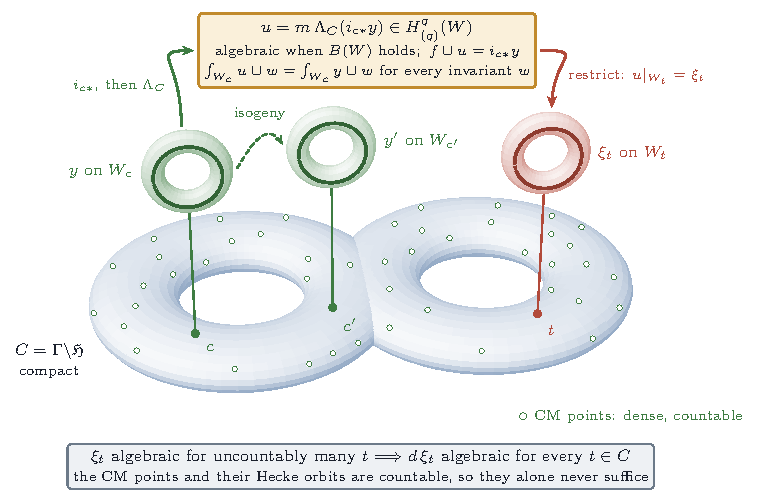
\includegraphics[width=0.84\textwidth]{fig_propagation}
\caption{\Cref{thm:lefschetzpropagation}(ii) along a compact Shimura curve
$C$. An algebraic class $y$ on one fibre, at a base point of a Weil family or
at a CM point of a Mumford family (hollow dots: the CM points, countable and
dense), is pushed into $W$ by the Gysin map and brought back to the invariant
summand by the base operator $\Lambda_{C}$. When $B(W)$ holds the result $u$
is an algebraic class on $W$, pinned down by the displayed pairing against the
invariant classes, and its restriction to a very general fibre is the
invariant part of $y$. The dashed arcs are isogenies between CM members along
Hecke orbits: they carry algebraic classes to algebraic classes but reach
only countably many points, and \Cref{lem:spreading}, in the box, needs
uncountably many. This is how \Cref{cor:weilequiv} and
\Cref{cor:mumfordequiv} turn each target into one case of \textup{(L)}.}
\label{fig:propagation}
\end{figure}

\begin{theorem}[The Mumford square at a CM point]\label{thm:mumfordcm}
Let $W\to C$ be a family as in \Cref{cor:mumfordlefschetz} and $c\in C$ a CM
point. Then every Hodge class on $X_{c}\times X_{c}$ is algebraic. In
particular the two exceptional classes of \Cref{prop:mumfordproduct} are
algebraic on $X_{c}\times X_{c}$.
\end{theorem}

\begin{proof}
The Hodge group $T$ of $X_{c}$ is a $\QQ$-torus contained in $G$. It lies in a
maximal $\QQ$-torus of $G=\Res_{F/\QQ}\SL_{1}(D)$, which is the restriction of
scalars of the norm one torus of a quadratic extension of $F$ inside $D$, of
rank three, one factor for each embedding of $F$. The cocharacter of the Hodge
structure lies in the factor of the embedding at which $D$ splits, and the
Galois group permutes the embeddings of $F$ transitively, so the smallest
$\QQ$-subtorus containing it has rank three: $T_{\CC}$ is a maximal torus of
$G_{\CC}\cong\SL_{2}^{3}$. Its eight weights on
$V=H^{1}(X_{c},\CC)=V_{1}\otimes V_{2}\otimes V_{3}$ are the vectors
$(\pm1,\pm1,\pm1)$, pairwise distinct. Hence
$\End^{0}(X_{c})\otimes\CC=\End_{T}(V)$ is the algebra of diagonal matrices
in a weight basis $(x_{w})$. For $n\ge1$, $\operatorname{Hom}(X_{c}^{n},X_{c})
\otimes\CC$ is the space of $n$-tuples $(\varphi_{1},\dots,\varphi_{n})$ of
such matrices, acting by $x_{w}\mapsto x_{w}\otimes u_{w}$ with
$u_{w}=(\varphi_{1,w},\dots,\varphi_{n,w})\in\CC^{n}$, so the vectors $u_{w}$
can be prescribed independently. The Hodge classes of $X_{c}^{n}$, tensored
with $\CC$, are spanned by the products of vectors $x_{w}\otimes u$,
$u\in\CC^{n}$, in $\bigwedge^{*}(V\otimes\CC^{n})$ in which the weights $w$,
counted with multiplicity, sum to zero.

We show that for every $n\ge1$ the ring $\Hdg^{*}(X_{c}^{n})$ is generated by
pull-backs of Hodge classes of $X_{c}$ along homomorphisms $X_{c}^{n}\to
X_{c}$. Put $w_{1}=(1,1,1)$, $w_{2}=(1,-1,-1)$, $w_{3}=(-1,1,-1)$ and
$w_{4}=(-1,-1,1)$; the weights are the $\pm w_{i}$,
$w_{1}+w_{2}+w_{3}+w_{4}=0$, and any three of the $w_{i}$ are linearly
independent, so the integer relations among them are the multiples of
$(1,1,1,1)$. Let $\alpha_{i}$ and $\beta_{i}$ be the multiplicities of $w_{i}$
and $-w_{i}$ in a nonempty multiset of weights with sum zero. Then
$\alpha_{i}-\beta_{i}$ is independent of $i$; so either some $\alpha_{i}$ and
$\beta_{i}$ are both positive, or all $\alpha_{i}$ are positive, or all
$\beta_{i}$ are. In each case the multiset contains one of the sets
$\{w_{i},-w_{i}\}$, $\{w_{1},w_{2},w_{3},w_{4}\}$,
$\{-w_{1},-w_{2},-w_{3},-w_{4}\}$, each of sum zero, and by induction every
product above is, up to sign, a product of monomials
$\bigwedge_{w\in P}(x_{w}\otimes u_{w})$ over such sets $P$, whose weights are
pairwise distinct. Choosing $f\in\Hom(X_{c}^{n},X_{c})\otimes\CC$ with
$f^{*}x_{w}=x_{w}\otimes u_{w}$ for $w\in P$ gives
$\bigwedge_{w\in P}(x_{w}\otimes u_{w})=f^{*}\bigl(\bigwedge_{w\in P}x_{w}\bigr)$,
with $\bigwedge_{w\in P}x_{w}$ a Hodge class of $X_{c}$ tensored with $\CC$.
The map $f\mapsto f^{*}(t)$ is polynomial and the rational homomorphisms are
Zariski dense in their complexification, so the same span is reached with $f$
defined over $\QQ$ and $t$ rational. The Hodge classes of the abelian fourfold
$X_{c}$ are algebraic because the Hodge conjecture holds for abelian fourfolds
\cite{Mar25a}, and pull-backs and products of algebraic classes are
algebraic. The case $n=2$ is the theorem.
\end{proof}

\begin{corollary}[The first classes beyond the Weil lines are one case of
\textup{(L)}]\label{cor:mumfordequiv}
Let $W\to C$ be as in \Cref{cor:mumfordlefschetz} and
$W^{(2)}=W\times_{C}W\to C$, an abelian scheme of relative dimension eight
with $W^{(2)}$ projective of dimension nine. The following are equivalent.
\begin{enumerate}[label=\textup{(\alph*)},leftmargin=2.6em,itemsep=2pt]
\item $B(W^{(2)})$ holds for the class $L_{W^{(2)}}$.
\item The two exceptional classes of $X_{t}\times X_{t}$ are algebraic for
  uncountably many $t\in C$.
\item The Hodge conjecture holds for $X_{t}\times X_{t}$ for every $t\in C$.
\item The Hodge conjecture holds for $W^{(2)}$; for this item $C$ is taken to
  be the compact Shimura curve of torsion-free level, or a finite \'etale
  cover of it.
\end{enumerate}
\end{corollary}

\begin{proof}
As in the proof of \Cref{cor:mumfordlefschetz}, the connected monodromy group
is $G$, so the monodromy invariants in $H^{*}(X_{t}\times X_{t},\QQ)$ are
contained in the $G$-invariants, which are the Hodge classes of
$X_{t}\times X_{t}$ for $t$ very general; conversely a $G$-invariant class is
flat, being fixed by the monodromy. The Hodge group of every fibre lies in
$G$, so the invariant classes are Hodge classes on every fibre. At a point $t$
that is not a CM point the Hodge group $H_{t}$ of $X_{t}$ is $G$. Indeed, if
$H_{t}$ were smaller, the Hodge classes of the powers of $X_{t}$ that are not
$G$-invariant would stay Hodge only on a discrete subset of the period
domain, the upper half plane; every point of the orbit of the Hodge structure
at $t$ under $H_{t}(\RR)^{+}$ carries them, so that orbit is a point, the
cocharacter of the Hodge structure is central in $H_{t}$, and $H_{t}$, the
smallest $\QQ$-group containing it, is a torus: $t$ would be a CM point. So
at such $t$ the Hodge classes of $X_{t}\times X_{t}$ are the invariant ones,
and $\End^{0}(X_{t})=\End_{G}(V)=\QQ$, because
$V\otimes\bar{\QQ}=V_{1}\otimes V_{2}\otimes V_{3}$ is an irreducible
representation of $G$; thus $X_{t}$ is as in \Cref{setup:mumford}.

(c) implies (b) trivially. (b) implies (c): the exceptional classes are
invariant, hence flat, so by \Cref{lem:spreading} a multiple of each is the
restriction of an algebraic class on $W^{(2)}$, and they are algebraic on
every fibre. At a point that is not a CM point, \Cref{thm:mumfordpowers} with
$n=2$ makes every Hodge class of $X_{t}\times X_{t}$ algebraic; at a CM point
this is \Cref{thm:mumfordcm}. (c) implies (a): by (c) every invariant class is
algebraic on every fibre, so by \Cref{lem:spreading} a multiple of it is the
restriction of an algebraic class on $W^{(2)}$, and
\Cref{thm:lefschetzfamily} gives $B(W^{(2)})$. (a) implies (c): at a CM point
$c_{0}$ every Hodge class of $X_{c_{0}}\times X_{c_{0}}$ is algebraic by
\Cref{thm:mumfordcm}, so by \Cref{thm:lefschetzpropagation}(iii) every
invariant class is the restriction of an algebraic class, and is algebraic on
every fibre. This is (c) at the points that are not CM points, where the
Hodge classes are the invariant ones; at a CM point (c) is
\Cref{thm:mumfordcm}.

For (d), split $H^{*}(W^{(2)},\QQ)$ into the summands $H^{p}(C,R^{q})$,
$p\in\{0,1,2\}$, as in the proof of \Cref{prop:mumfordfivefold}. The summands
with $p=1$ carry no Hodge class, by the argument given there, applied to the
fibre square. Those with $p=2$ are $f\cup H^{q}_{(q)}$, and
$f\cup u=i_{c*}(u|_{W^{(2)}_{c}})$ for any $c$; taking $c$ a CM point, where
$u|_{W^{(2)}_{c}}$ is a Hodge class and so algebraic by \Cref{thm:mumfordcm},
they are algebraic. The summands with $p=0$ are the invariants, all of Hodge
type. So (d) holds exactly when every invariant class is the restriction of an
algebraic class, which by \Cref{thm:lefschetzpropagation}(iii), applied at a
CM point, is (a).
\end{proof}

\begin{corollary}[One Weil family is one case of \textup{(L)}]
\label{cor:weilequiv}
Keep \cite[Setup~16.1]{paperI}, let $s_{0}\in\cS$ be the image of a base point of
\cite[Theorem~15.27]{paperI}, and let $t_{1}\in\cS$ lie outside every proper
Zariski closed set $\Sigma_{\underline{P},\underline{q}}$ of
\cite[Theorem~16.4]{paperI}. Let $\kappa\colon C\to\cS$ be a morphism from a smooth
projective connected curve whose image contains $s_{0}$ and $t_{1}$, and
$W_{C}=\cA\times_{\cS}C$.
\begin{enumerate}[label=\textup{(\roman*)},leftmargin=2.6em,itemsep=2pt]
\item If $B(W_{C})$ holds for $L_{W_{C}}$, then $\Sigma=\cD_{n,n}$, and the
  Hodge conjecture holds in every degree for every member of the family with
  $\Hg(A)=\SU(V,H)$.
\item Conversely, if $\Sigma=\cD_{n,n}$ and the monodromy of $W_{C}$ is Zariski
  dense in $\SU(V,H)$, then $B(W_{C})$ holds for $L_{W_{C}}$.
\end{enumerate}
\end{corollary}

\begin{proof}
(i) The class $\kappa^{*}\omega$ is a global section of
$R^{2n}\pi_{*}\QQ$ on $C$, algebraic at a point over $s_{0}$ by
\cite[Theorem~15.27]{paperI}. By \Cref{thm:lefschetzpropagation}(ii) it is algebraic
at a point over $t_{1}$, so $t_{1}$ lies in some closed set
$\Sigma_{\underline{P},\underline{q}}$, which is therefore all of $\cS$.
\cite[Theorem~16.4]{paperI} gives $\Sigma=\cD_{n,n}$, and \cite[Theorem~15.14(a)]{paperI}
the rest. (ii) With dense monodromy the invariants are the
$\SU(V,H)$-invariants, which are the Hodge classes of a member with
$\Hg(A)=\SU(V,H)$: the powers of the polarisation and the Weil classes, by
\cite[Theorem~4.14]{paperI}. All are algebraic on every fibre when
$\Sigma=\cD_{n,n}$, so they are restrictions of algebraic classes by
\Cref{lem:spreading}, and \Cref{thm:lefschetzfamily} applies.
\end{proof}

Curves $\kappa$ as in \Cref{cor:weilequiv} exist: the Baily--Borel
compactification of $\cS$ is projective \cite{BB66}, its boundary has
codimension $2n-1\ge3$, the rational boundary components of the domain of type
$\mathrm{I}_{n,n}$ being of type $\mathrm{I}_{n-r,n-r}$ with $r\ge1$, and a
general complete intersection curve through $s_{0}$ and $t_{1}$ avoids it.

\begin{theorem}[Two branches cannot be two objects]\label{thm:nosum}
Let $A$ be of $(K,-1,n)$-Weil type with $n\ge2$, $\omega\ne0$ a rational class
on the Weil line, and $E$ a perfect complex with $\ch(E)=N\omega$, $N\ne0$, and
$\sigma_{E}$ injective. Let
$E\cong\bigoplus_{i}F_{i}[k_{i}]$ be any decomposition. Then every summand
$F_{i}$ with $\ch(F_{i})\ne0$ has a Yoneda product
$\bigwedge^{2}\Ext^{1}(F_{i},F_{i})\to\Ext^{2}(F_{i},F_{i})$ that is not
injective. In particular $E$ is not a direct sum of shifts of line bundles,
of skyscraper sheaves of points, or of their images under autoequivalences of
$D^{b}(A)$, since the Ext algebra of each of these is the exterior algebra on
its $\Ext^{1}$.
\end{theorem}

\begin{proof}
By \cite[Theorem~2.11(ii)]{paperII} the kernel of $\operatorname{ev}_{E}$ in degree
two is $P\wedge Q$. The characteristic morphism is compatible with the
decomposition, so $\operatorname{ev}_{F_{i}}(p\wedge q)=
\operatorname{ev}_{F_{i}}(p)\operatorname{ev}_{F_{i}}(q)=0$ for all
$p\in P$ and $q\in Q$. Suppose the Yoneda product of $F=F_{i}$ is injective on
$\bigwedge^{2}\Ext^{1}$. Then the images $\bar P$ and $\bar Q$ of $P$ and $Q$
in $\Ext^{1}(F,F)$ satisfy $\bar p\wedge\bar q=0$ for all $\bar p,\bar q$, so
either $\bar P=0$, or $\bar Q=0$, or $\bar P=\bar Q$ is a line. In the first
case $\operatorname{ev}_{F}$ kills $P\wedge HH^{1}$, in the second
$Q\wedge HH^{1}$, in the third all of $HH^{2}=HH^{1}\wedge HH^{1}$; by the
compatibility $\sigma_{F}\circ\operatorname{ev}_{F}=(\,\cdot\,)\lrcorner
\ch(F)$ of \cite[Setup~2.7]{paperII} the same subspace annihilates $x=\ch(F)$.

These annihilators are computed in the free module of rank one that
$H^{*}(A,\CC)$ is over $HH^{*}(A)=\bigwedge^{*}(P\oplus Q)$, with generator the
holomorphic volume form $\Omega$: an element $y\cdot\Omega$ is killed by
$P\wedge HH^{1}$ exactly when $p\wedge y$ has top degree for every $p\in P$,
that is when $y\in\det P\wedge\bigwedge^{*}Q+\bigwedge^{\ge4n-1}(P\oplus Q)$.
Since $\det P\cdot\Omega=\pm\alpha_{+}$, the first summand gives the classes
$\bigwedge^{j}Q\cdot\alpha_{+}$, of type $(n-b,n+a)$ with $a$ wedges by
$V_{-}^{0,1}$ and $b$ contractions by $T_{+}$, and the second gives classes of
type $(1,2n)$, $(0,2n-1)$ and $(0,2n)$. The components of $x$ are of type
$(k,k)$, so $x\in\CC\alpha_{+}$. Symmetrically the second case gives
$x\in\CC\alpha_{-}$ and the third $x=0$. Finally $x$ is
rational, complex conjugation carries $V_{+}$ to $V_{-}$ and $H^{1,0}$ to
$H^{0,1}$, so $\bar\alpha_{+}\in\CC\alpha_{-}$, and a rational multiple of
$\alpha_{+}$ or of $\alpha_{-}$ is zero. So $\ch(F)=0$. As
$\sum_{i}(-1)^{k_{i}}\ch(F_{i})=N\omega\ne0$, some summand has nonzero
Chern character, and the first statement follows; the second is the special
case in which every summand has an exterior Ext algebra.
\end{proof}

\subsection{Which hypotheses suffice}
\label{ssec:closure}

The implications proved above, together with those of \Cref{ssec:bullseye},
determine exactly which combinations of statements yield the conjecture. The
logical skeleton of the paper and of the literature it quotes is finite: a
set of statements, each of them proved here, quoted from the literature, or
taken as a hypothesis, and a set of inference rules, each of them one
theorem. Consequences can then be taken.

The answer is only as strong as the rule set. A set of statements the rules
do not carry to the conjecture is \emph{insufficient} in the sense of the
rules, and that means no more than that no rule derives the conjecture from
it. An implication that is true and left out makes a set look necessary when
it is not. One such implication
is elementary, and it decides the shape of the answer, so we prove it first.

\begin{proposition}[The conjecture for the varieties that are not abelian
is the conjecture]\label{prop:f3ishc}
Let $A$ be a complex abelian variety of dimension $g\ge1$ and let
$X=A\times\PP^{1}$. Then $X$ is a smooth complex projective variety that is
not an abelian variety, and if every Hodge class of degree $2p$ on $X$ is
algebraic, then so is every Hodge class of degree $2p$ on $A$. Consequently
the statement
\begin{quote}
the Hodge conjecture holds for every smooth complex projective variety that
is not an abelian variety
\end{quote}
implies the Hodge conjecture for every abelian variety, and it is equivalent
to $\mathbf{HC}$.
\end{proposition}

\begin{proof}
$X$ is smooth and projective of dimension $g+1$. By the K\"unneth formula
$h^{1,0}(X)=h^{1,0}(A)+h^{1,0}(\PP^{1})=g$, while an abelian variety of
dimension $g+1$ has $h^{1,0}=g+1$; so $X$ is not an abelian variety. (Equally,
$X$ contains the rational curves $\{a\}\times\PP^{1}$, and every morphism
from $\PP^{1}$ to a complex torus is constant, since it lifts to the
universal cover $\CC^{g+1}$ \cite[Chapter~1]{BL04}.)

Let $\mathrm{pr}\colon X\to A$ be the projection and $D=A\times\{0\}$, a
smooth divisor that $\mathrm{pr}$ maps isomorphically onto $A$, so that
$\mathrm{pr}_{*}[D]=1$ in $H^{0}(A,\QQ)$. Let $\alpha$ be a Hodge class of
degree $2p$ on $A$. Pull-back along a morphism is a morphism of Hodge
structures, so $\mathrm{pr}^{*}\alpha$ is a Hodge class of degree $2p$ on
$X$, and by hypothesis $\mathrm{pr}^{*}\alpha=[Z]$ for an algebraic cycle
$Z$ on $X$ with rational coefficients. The projection formula gives
\[
  \mathrm{pr}_{*}\bigl([Z]\cup[D]\bigr)
  =\mathrm{pr}_{*}\bigl(\mathrm{pr}^{*}\alpha\cup[D]\bigr)
  =\alpha\cup\mathrm{pr}_{*}[D]=\alpha .
\]
The cycle class map is compatible with intersection products and with proper
push-forward \cite[Chapter~19]{Ful98}, so the left side
is the class of the cycle $\mathrm{pr}_{*}(Z\cdot D)$ and $\alpha$ is
algebraic. A point, the abelian variety of dimension zero, satisfies the
conjecture trivially.

So the displayed statement gives the conjecture for every abelian variety,
and with it the conjecture for every smooth complex projective variety. The
converse is immediate: the displayed statement is a special case of
$\mathbf{HC}$.
\end{proof}

Since the conjecture for the varieties that are not abelian is the whole
conjecture, the statement that belongs on a frontier is weaker: it asks for
algebraicity only modulo what abelian varieties supply.

\begin{definition}[The conjecture modulo abelian varieties]
\label{def:f3prime}
For a smooth complex projective variety $X$ and $p\ge0$ let
$\mathrm{Ab}^{p}(X)\subseteq H^{2p}(X,\QQ)$ be the span of the classes
$\Gamma_{*}\gamma=\mathrm{pr}_{X*}\bigl([\Gamma]\cup\mathrm{pr}_{B}^{*}\gamma\bigr)$
of degree $2p$, where $B$ runs over the complex abelian varieties, the point
included, $\gamma$ over the Hodge classes on $B$, and $\Gamma$ over the
algebraic cycles on $B\times X$ with rational coefficients. The statement
\textup{(F3$'$)} is: for every $X$ and every $p$,
\[
  \Hdg^{p}(X)=\mathrm{Ab}^{p}(X).
\]
\end{definition}

Each $\Gamma_{*}\gamma$ is a Hodge class, since cup product with an
algebraic class and push-forward preserve Hodge classes, so
$\mathrm{Ab}^{p}(X)\subseteq\Hdg^{p}(X)$; and taking $B$ a point shows that
$\mathrm{Ab}^{p}(X)$ contains every algebraic class. So \textup{(F3$'$)} says
that every Hodge class is algebraic modulo the images of Hodge classes of
abelian varieties under algebraic correspondences, which is the form of (F3)
that \Cref{rem:f3collapse} asks for.

\begin{proposition}[What is known of \textup{(F3$'$)}]\label{prop:f3prime}
\leavevmode
\begin{enumerate}[label=\textup{(\roman*)},leftmargin=2.6em]
\item $\mathbf{HC}$ implies \textup{(F3$'$)}, and \textup{(F3$'$)} together
  with the conjecture for abelian varieties implies $\mathbf{HC}$.
\item \textup{(F3$'$)} holds on every abelian variety and on every product
  $A\times\PP^{1}$ with $A$ abelian; the argument of \Cref{prop:f3ishc} gives
  nothing for it.
\item Let $\mathcal{A}$ be the class of smooth complex projective varieties
  $X$ for which $H^{*}(X,\QQ)$ is spanned by classes $\Gamma_{*}y$ with $B$
  abelian, $\Gamma$ an algebraic cycle on $B\times X$ and
  $y\in H^{*}(B,\QQ)$. Every $X\in\mathcal{A}$ satisfies \textup{(F3$'$)}.
  The class $\mathcal{A}$ contains every abelian variety and every smooth
  projective curve, and it is closed under products and under images of
  surjective morphisms. So it contains every product of curves, every
  symmetric product of a curve, and every smooth projective variety onto
  which a product of curves or an abelian variety maps surjectively.
\item Every $X$ of dimension $n$ satisfies \textup{(F3$'$)} in the degrees
  $2p$ with $p\in\{0,1,n-1,n\}$, so every $X$ of dimension at most three
  satisfies it in every degree.
\end{enumerate}
\end{proposition}

\begin{proof}
(i) If $\mathbf{HC}$ holds, then $\Hdg^{p}(X)$ consists of algebraic classes,
which lie in $\mathrm{Ab}^{p}(X)$. Conversely, if the conjecture holds for
abelian varieties, every $\gamma$ in \Cref{def:f3prime} is algebraic, so
every $\Gamma_{*}\gamma$ is, since composition with a correspondence carries
algebraic classes to algebraic classes \cite[Chapter~16]{Ful98}; then
\textup{(F3$'$)} says that every Hodge class is algebraic.

(ii) On an abelian variety $A$ take $B=A$ and $\Gamma$ the diagonal. On
$X=A\times\PP^{1}$ the K\"unneth formula gives
$H^{*}(X,\QQ)=\mathrm{pr}^{*}H^{*}(A,\QQ)\oplus
\mathrm{pr}^{*}H^{*}(A,\QQ)\cup\eta$, with $\eta$ the class of a point of
$\PP^{1}$ pulled back to $X$, which is algebraic. The first summand is
$\Gamma_{*}H^{*}(A,\QQ)$ for $\Gamma$ the transpose of the graph of
$\mathrm{pr}$, and the second is $\Gamma'_{*}H^{*}(A,\QQ)$ for
$\Gamma'=\Gamma\cdot\mathrm{pr}_{X}^{*}\eta$. So $X\in\mathcal{A}$, and
(iii) applies.

(iii) Let $X\in\mathcal{A}$ and fix $p$. Since $H^{2p}(X,\QQ)$ is finite
dimensional, finitely many classes $\Gamma_{j*}y_{j}$ span it, and we may
take each $\Gamma_{j}$ of pure codimension $c_{j}$ on $B_{j}\times X$ and each
$y_{j}$ of pure degree $k_{j}$, with $k_{j}+2c_{j}-2\dim B_{j}=2p$. Then
$\Gamma_{j*}\colon H^{k_{j}}(B_{j},\QQ)\to H^{2p}(X,\QQ)$ is a morphism of
Hodge structures up to a Tate twist, and the sum of these maps is a
surjective morphism of polarisable Hodge structures onto $H^{2p}(X,\QQ)$.
Polarisable Hodge structures are semisimple, so its kernel has a complement
that is a sub-Hodge structure and maps isomorphically onto $H^{2p}(X,\QQ)$;
hence every Hodge class of degree $2p$ is the image of a Hodge class, that is
$\sum_{j}\Gamma_{j*}\gamma_{j}$ with each $\gamma_{j}$ a Hodge class on
$B_{j}$. So $\Hdg^{p}(X)=\mathrm{Ab}^{p}(X)$.

An abelian variety lies in $\mathcal{A}$ through its diagonal. A curve $C$
of genus $g\ge1$ lies in $\mathcal{A}$ through an Abel--Jacobi embedding
$\iota\colon C\to J(C)$: the transpose of its graph induces $\iota^{*}$,
which is an isomorphism on $H^{0}$ and $H^{1}$ and sends the class of the
theta divisor to $g$ times the class of a point, so it is surjective; the
projective line is the image of an elliptic curve under a double cover, and
is covered by the last closure property. For products, if $H^{*}(X_{i},\QQ)$
is spanned by the $\Gamma_{i*}y$, then by the K\"unneth formula
$H^{*}(X_{1}\times X_{2},\QQ)$ is spanned by the
$(\Gamma_{1}\times\Gamma_{2})_{*}(y_{1}\otimes y_{2})$, with
$\Gamma_{1}\times\Gamma_{2}$ an algebraic cycle on
$(B_{1}\times B_{2})\times(X_{1}\times X_{2})$. For images, let
$f\colon Y\to X$ be a surjective morphism with $Y\in\mathcal{A}$, let
$r=\dim Y-\dim X$ and let $h$ be an ample class on $Y$. The correspondence
$\Psi=[\Gamma_{f}]\cdot\mathrm{pr}_{Y}^{*}h^{r}$ on $Y\times X$ induces
$\Psi_{*}y=f_{*}(y\cup h^{r})$, and
$\Psi_{*}f^{*}x=x\cup f_{*}h^{r}=c\,x$ with $c>0$ the degree of $h^{r}$ on a
general fibre. So $\Psi_{*}$ is surjective, and $H^{*}(X,\QQ)$ is spanned by
the classes $(\Psi\circ\Gamma)_{*}y$, with $\Psi\circ\Gamma$ algebraic
\cite[Chapter~16]{Ful98}. A symmetric product of a curve is the image of a
power of it.

(iv) Every class of degree $0$ or $2n$ is algebraic, and every Hodge class of
degree $2$ is algebraic by the Lefschetz theorem on $(1,1)$ classes. For
$n\ge2$, the hard Lefschetz theorem makes cup product with $h^{n-2}$, for $h$
an ample class, an isomorphism $H^{2}(X,\QQ)\to H^{2n-2}(X,\QQ)$ of Hodge
structures up to a Tate twist, so every Hodge class of degree $2n-2$ is
$h^{n-2}$ times a Hodge class of degree $2$, and is algebraic. Algebraic
classes lie in $\mathrm{Ab}^{p}(X)$. When $n\le3$ every $p$ between $0$ and
$n$ is one of $0,1,n-1,n$.
\end{proof}

\begin{remark}[The reach of algebraic correspondences]\label{rem:f3primeopen}
\textup{(F3$'$)} is the statement that the Hodge conjecture reduces to
abelian varieties along algebraic correspondences, and
\Cref{prop:f3prime} records the cases of such a reduction that are theorems:
the varieties of $\mathcal{A}$, whose whole cohomology is reached from abelian
varieties by algebraic correspondences, and the degrees in which the
conjecture itself is a theorem. The next degree is degree four on fourfolds
outside $\mathcal{A}$ and outside the scope of \Cref{prop:f3primesmall} and
\Cref{prop:f3primefibration}. The square $S\times S$ of a K3 surface is the standard
example when $\End_{\mathrm{Hdg}}(T(S))$ is a totally real field of degree
at least two, that is, when $S$ has real multiplication. When that field is
$\QQ$ or a CM field, the Hodge conjecture holds on $S\times S$: by
\Cref{prop:orthpowers}(i) in the first case, and in the second by
\cite{Bus19} and the fact that the elements of norm one span a CM field, as in
\cite{RM08} (\Cref{prop:k3powers}). Its Hodge classes in
$H^{2}(S)\otimes H^{2}(S)$ include the classes
that induce the Hodge endomorphisms of the transcendental lattice $T(S)$, and
$S\times S$ lies in $\mathcal{A}$ as soon as the Kuga--Satake embedding of
$T(S)$ is induced by an algebraic cycle, the Kuga--Satake Hodge conjecture for
$S$: the transpose of such a cycle maps the
cohomology of the Kuga--Satake variety onto $T(S)$, and the rest of
$H^{*}(S,\QQ)$ is algebraic. The rational Hodge isometries are algebraic
\cite{Bus19}, but a real multiplication is not an isometry, and
\Cref{rem:mumfordks} meets exactly this obstacle for the surfaces
$S_{\lambda}$; the dihedral family of correspondences of \cite{BB26dense} crosses it
for two cyclic cubic fields and reaches no other field.

For varieties whose cohomology is not of abelian type the position is
starker. By \Cref{prop:noabeliantype} no correspondence moves the $H^{3}$ of a
very general quintic threefold into the cohomology of an abelian variety, so
such a variety does not lie in $\mathcal{A}$. That is no obstruction to
\textup{(F3$'$)} itself, since a Hodge class spans a Hodge structure of Tate
type, which is of abelian type, and nothing in Hodge theory forbids it from
lying in $\mathrm{Ab}^{p}(X)$. Nor is it a route: to put a Hodge class into
$\mathrm{Ab}^{p}(X)$ one must construct an algebraic cycle on $B\times X$
whose class carries it, which is the kind of construction the Hodge
conjecture asks for, now on $B\times X$ instead of on $X$. The cases of
\textup{(F3$'$)} proved below outside $\mathcal{A}$ come from the Hodge
conjecture itself, from hypotheses on zero-cycles, and, in degree four, from
correspondences with members of $\mathcal{A}$
(\Cref{prop:k3powers} to \Cref{prop:f3primedominant}); none of them reaches a
variety in general position, and \textup{(F3$'$)} enters \Cref{thm:closure} as
a hypothesis.
\end{remark}

Two further facts fix the position of \textup{(F3$'$)}. The first says how
strong it is.

\begin{proposition}[The strength of \textup{(F3$'$)}]\label{prop:f3primestrength}
\textup{(F3$'$)} implies \textup{(M)}: every Hodge class on every smooth
complex projective variety is motivated in the sense of Andr\'e. In
particular it implies that every such class is absolutely Hodge. Adding the
implication $\textup{(F3$'$)}\Rightarrow\textup{(M)}$ to the rule set of
\Cref{setup:rules} leaves the five minimal sufficient sets of
\Cref{thm:closure}(ii) unchanged.
\end{proposition}

\begin{proof}
Let $\gamma\in\Hdg^{p}(X)$. By \textup{(F3$'$)},
$\gamma=\sum_{j}\Gamma_{j*}\beta_{j}$ with $\beta_{j}$ a Hodge class on an
abelian variety $B_{j}$ and $\Gamma_{j}$ an algebraic cycle on $B_{j}\times X$.
Every Hodge class on an abelian variety is motivated
\cite[Th\'eor\`eme~0.6.2]{And96b}, and the motivated classes form a graded
$\QQ$-algebra that contains the algebraic classes and is stable under
pull-back and push-forward along morphisms \cite[\S2]{And96b}. So
$\mathrm{pr}_{B_{j}}^{*}\beta_{j}\cup[\Gamma_{j}]$ is motivated, and so is its
push-forward $\Gamma_{j*}\beta_{j}$; hence $\gamma$ is motivated. Motivated
classes are absolutely Hodge \cite[\S2]{And96b}. For the last assertion,
the new rule has the premise (F3$'$) and the conclusion (M). The sets $C_{1}$
and $C_{2}$ of the proof of \Cref{thm:closure} omit (F3$'$), and $C_{3}$ and
$C_{4}$ contain both statements, so the four sets stay closed and that proof
applies without change; the five sets remain sufficient, since adding a rule
only enlarges closures.
\end{proof}

So on the route $\{\mathrm{L},\mathrm{F3}'\}$ the second member already
contains \textup{(M)}, and that route is never easier than
$\{\mathrm{L},\mathrm{M}\}$. The second fact locates, on the powers of a variety of orthogonal type,
the first class that \textup{(F3$'$)} has to reach.

\begin{proposition}[Powers of a variety of orthogonal type]
\label{prop:orthpowers}
Let $Y$ be a smooth complex projective variety of even dimension $m$. Suppose
that $H^{k}(Y,\QQ)$ is spanned by algebraic classes for $k\ne m$, that
$H^{m}(Y,\QQ)=N\oplus V$ with $N$ spanned by algebraic classes, the
intersection form $\psi$ nondegenerate on $N$ and $V=N^{\perp}$, and that the
Hodge group of $V$ is $\SO(V,\psi)$, with $t=\dim V\ge3$. Let
$\det(V)\in H^{mt}(Y^{t},\QQ)$ be the image of a generator of
$\bigwedge^{t}V\subseteq V^{\otimes t}$ under the K\"unneth embedding
$V^{\otimes t}\subseteq H^{mt}(Y^{t},\QQ)$.
\begin{enumerate}[label=\textup{(\roman*)},leftmargin=2.6em,itemsep=2pt]
\item The Hodge conjecture holds for $Y^{n}$ for every $n<t$.
\item $\det(V)$ is a Hodge class, and $\Hdg^{*}(Y^{t})$ is spanned by
  algebraic classes and $\det(V)$.
\item $\det(V)$ does not lie in the $\QQ$-algebra generated by the pull-backs
  along the projections of the Hodge classes of the $Y^{j}$, $j<t$.
\item The Hodge conjecture holds for every power of $Y$ if and only if
  $\det(V)$ is algebraic, and \textup{(F3$'$)} holds for every power of $Y$
  if and only if $\det(V)\in\mathrm{Ab}(Y^{t})$.
\end{enumerate}
\end{proposition}

\begin{proof}
Algebraic classes have even degree, so $H^{k}(Y,\QQ)=0$ for odd $k$. Let
$[\Delta]=\sum_{k}\pi_{k}$ be the K\"unneth decomposition of the class of the
diagonal, $\pi_{k}\in H^{2m-k}(Y,\QQ)\otimes H^{k}(Y,\QQ)$. For $k\ne m$,
$\pi_{k}=\sum_{i}e_{i}^{\vee}\otimes e_{i}$ for a basis $(e_{i})$ of
$H^{k}(Y,\QQ)$ and the Poincar\'e dual basis of $H^{2m-k}(Y,\QQ)$, both
spanned by algebraic classes, so $\pi_{k}$ is algebraic; likewise the part
$\pi_{N}$ of $\pi_{m}$ in $N\otimes N$, since $\psi$ is nondegenerate on $N$.
So $\pi_{V}=[\Delta]-\sum_{k\ne m}\pi_{k}-\pi_{N}$, the class of $\psi^{-1}$ in
$V\otimes V\subseteq H^{2m}(Y\times Y,\QQ)$, is algebraic.

The Hodge group of $Y^{n}$ is $\SO(V,\psi)$, acting on
$H^{*}(Y^{n},\QQ)=\bigl(H^{*}(Y,\QQ)\bigr)^{\otimes n}$ through the factors $V$
and trivially on the rest, which is spanned by algebraic classes; so the Hodge
classes are the $\SO(V)$-invariants. By the first fundamental theorem for the
special orthogonal group \cite[Chapter~5]{GW09}, the invariants of $\SO(V)$ in
$V^{\otimes j}$ are spanned by the complete contractions with $\psi^{-1}$ when
$j<t$, and, when $j=t$, by these and the determinant tensor; in general they
are spanned by products of contractions and determinant tensors on disjoint
sets of $t$ factors. A contraction of the factors $a$ and $b$ of $Y^{n}$ is the
pull-back of $\pi_{V}$ along the projection to those two factors, a
determinant on a set $I$ of $t$ factors is the pull-back of $\det(V)$ along
the projection to $Y^{I}$, and products of these with pull-backs of algebraic
classes span the Hodge classes. This gives (i), (ii) and the first half of
(iv). For (iii), the orthogonal group $\mathrm{O}(V,\psi)$ acts on
$H^{*}(Y^{j},\QQ)$ in the same way, and for $j<t$ every $\SO(V)$-invariant is
$\mathrm{O}(V)$-invariant; pull-backs along projections and cup products
commute with the diagonal action of $\mathrm{O}(V)$, so every element of the
algebra in (iii) is $\mathrm{O}(V)$-invariant, while a reflection acts on
$\det(V)$ by $-1$. For the second half of (iv), $\mathrm{Ab}^{*}(Y^{n})$
contains the algebraic classes and is stable under pull-back along projections
and under cup product: $\Gamma_{*}\gamma\cup\Gamma'_{*}\gamma'$ is the image of
$\gamma\otimes\gamma'$ on $B\times B'$ under the correspondence
$(\Gamma\times\Gamma')$ followed by the diagonal of $Y^{n}$.
\end{proof}

For a K3 surface $S$ with $\End_{\mathrm{Hdg}}(T(S))=\QQ$ the Hodge group of
$T(S)$ is $\SO(T(S))$ \cite{Zar83}; for a very general one, $t=21$. So the
Hodge conjecture holds for $S^{n}$ with $n\le20$, and on $S^{21}$ it is
equivalent to the algebraicity of the single class $\det(T(S))$. The argument
is the classical one from invariant theory, and we make no claim of priority
for it. What it adds here is the location of the first instance of
\textup{(F3$'$)} on the powers of such a variety that invariant theory does
not reach: one class, in one degree, on one power.

The same invariant theory, with the motivic decompositions of the
literature and the theorems of Buskin and Markman on Hodge isometries, gives
the Hodge conjecture itself, and so \textup{(F3$'$)}, on the other varieties
built from a K3 surface and on varieties of K3$^{[n]}$ type, up to a real
multiplication and one determinant class.

\begin{proposition}[Powers, Hilbert schemes and moduli spaces of a K3
surface]\label{prop:k3powers}
Let $S$ be a projective K3 surface, $T=T(S)_{\QQ}$, $t=\dim T$ and
$E=\End_{\mathrm{Hdg}}(T)$, a totally real field or a CM field \cite{Zar83}.
\begin{enumerate}[label=\textup{(\roman*)},leftmargin=2.6em,itemsep=2pt]
\item If $E$ is a CM field, the Hodge conjecture holds for every power
  $S^{k}$ \cite[Theorem~5.4]{RM08}, \cite{Bus19}, hence for every Hilbert
  scheme $S^{[n]}$ \cite{dCM02}, for every smooth projective moduli space of
  Gieseker stable (twisted) sheaves on $S$, or of $\sigma$-stable objects in
  $D^{b}(S,\alpha)$ for a generic stability condition $\sigma$ and a Brauer
  class $\alpha$ \cite[Theorem~0.1, Remark~2.1]{Bue20}, and for the crepant
  resolutions of the ten-dimensional moduli spaces $M_{\sigma}(2v_{0})$ of
  $\sigma$-semistable objects in $D^{b}(S,\alpha)$, with $v_{0}$ primitive,
  $v_{0}^{2}=2$ and $\sigma$ $v_{0}$-generic \cite[Theorem~1.3]{FFZ21}.
\item If $E=\QQ$, the Hodge conjecture holds for $S^{[n]}$ for every
  $n<t(t+1)/2$, and for every moduli space $M$ as in \textup{(i)} with
  $\dim M<t$. For $N=t(t+1)/2$ the following are equivalent: the Hodge
  conjecture for $S^{[N]}$; the algebraicity of the class $\det(T)$ on $S^{t}$
  of \Cref{prop:orthpowers}; the Hodge conjecture for every power of $S$; and
  the Hodge conjecture for every $S^{[n]}$. For a very general $S$, the Hodge
  conjecture holds for $S^{[n]}$ with $n\le230$, and for $S^{[231]}$ if and
  only if $\det(T(S))$ on $S^{21}$ is algebraic.
\item If $E$ is totally real of degree at least two, the Hodge conjecture for
  $S\times S$, the Hodge conjecture for $S^{[2]}$, and the statement that
  every element of $E$ acts on $T$ through an algebraic cycle on $S\times S$
  are equivalent.
\end{enumerate}
Wherever the Hodge conjecture holds, so does \textup{(F3$'$)}. This is a
consequence of \cite{RM08,Bus19,dCM02,Bue20,FFZ21} and
\Cref{prop:orthpowers}; we make no claim of priority.
\end{proposition}

\begin{proof}
We use three facts. First, $H^{*}(S,\QQ)=A\oplus T$ with
$A=H^{0}\oplus\NS(S)_{\QQ}\oplus H^{4}$ spanned by algebraic classes; the
K\"unneth components of the diagonal of $S$ are algebraic \cite{Mur90}, and
so is its part $\pi_{T}$ in $T\otimes T$, as in the proof of
\Cref{prop:orthpowers}. The Hodge classes of $S^{k}$ are the invariants in
$(A\oplus T)^{\otimes k}$ of the Hodge group of $T$, which acts trivially on
$A$. Second, if $H^{*}(X,\QQ)$ is spanned by the images of the
$H^{*}(Y_{i},\QQ)$ under algebraic correspondences and the Hodge conjecture
holds for every $Y_{i}$, it holds for $X$: by the semisimplicity argument of
the proof of \Cref{prop:f3prime}(iii) every Hodge class of $X$ is a sum of
images of Hodge classes of the $Y_{i}$. Third, the correspondences
$\Gamma_{\nu}$ of the proof of \Cref{prop:aclosure}(ii) give an isomorphism
of Chow motives between $h(S^{[n]})$ and
$\bigoplus_{\nu}h(S^{(\nu)})(l(\nu)-n)$ \cite{dCM02}, so each
$h(S^{(\nu)})(l(\nu)-n)$ is a direct summand of $h(S^{[n]})$, and the lift
$\widetilde\Gamma_{\nu*}$ takes the same value on a class of $S^{l(\nu)}$ and
on its average over $G_{\nu}$. Hence the Hodge
conjecture holds for $S^{[n]}$ if and only if, for every partition $\nu$ of
$n$, every $G_{\nu}$-invariant Hodge class of $S^{l(\nu)}$ is algebraic. By
\cite[Theorem~0.1, Remark~2.1]{Bue20} the Chow motive of a moduli space $M$
as in (i) is a direct summand of a sum of Tate twists of motives
$h(S^{k_{i}})$ with $1\le k_{i}\le\dim M$, and by
\cite[Corollary~4.5]{FFZ21} the Chow motive of a crepant resolution as in (i)
lies in the tensor subcategory generated by $h(S)$, whose objects are direct
summands of sums of
Tate twists of the $h(S^{k})$, the dual of $h(S)$ being $h(S)(2)$.

(i) Over $\CC$ the Hodge group of $T$ is a product of groups
$\GL(W_{\sigma})$ acting on
$T_{\CC}=\bigoplus_{\sigma}(W_{\sigma}\oplus W_{\sigma}^{\vee})$
\cite{Zar83}, and by the first fundamental theorem for the general linear
group \cite[Chapter~5]{GW09} its invariants in $T_{\CC}^{\otimes b}$ are
spanned by products of contractions of one factor with another. Under the
isomorphism $\End(T)\cong T\otimes T$, $\varphi\mapsto\tau_{\varphi}=
\sum_{i}t_{i}^{\vee}\otimes\varphi(t_{i})$, with $(t_{i}^{\vee})$ the dual
basis of a basis $(t_{i})$ for the intersection form, the Hodge classes of
$T\otimes T$ are the $\tau_{\varphi}$ with $\varphi\in E$, and these
contractions lie in their complex span. The rational span of the products of
the $\tau_{\varphi}$ on pairs of factors has the same complexification as the
space of invariants, so the Hodge classes of $S^{k}$ are spanned by such
products and pull-backs of algebraic classes. For $u\in E$ with $u\bar u=1$
the map $\id_{\NS}\oplus u$ is a rational Hodge isometry of
$H^{2}(S,\QQ)$, since the adjoint of $u$ is $\bar u$ \cite{Zar83}; it is
induced by an algebraic cycle \cite{Bus19}, and composing that cycle with
$\pi_{T}$ on both sides gives $\tau_{u}$, which is therefore algebraic. The
elements of norm one span $E$. Indeed, write $E=E_{0}(y_{0})$ with
$y_{0}^{2}=-\delta$, $\delta\in E_{0}$, and let $y\in E$ with $\bar y=-y$; for
$s\in\QQ$ the element $u_{s}=(1+sy)(1-sy)^{-1}$ has norm one. A linear form
on $E$ vanishing on all $u_{s}$ gives a rational function of $s$ vanishing on
$\QQ$, so it vanishes on the coefficients $1$, $2y$, $2y^{2}$ of the expansion
of $u_{s}$ in powers of $s$. As $y$ runs over $E_{0}y_{0}$, the $y$ span
$E_{0}y_{0}$ and the $y^{2}=-a^{2}\delta$, $a\in E_{0}$, span $E_{0}$, since
$2a=(a+1)^{2}-a^{2}-1$. So every $\tau_{u}$, $u\in E$, is algebraic, and the
Hodge conjecture holds for every $S^{k}$; this is the argument of
\cite[Lemma~5.3, Theorem~5.4]{RM08}, which takes the algebraicity of the
isometries from Mukai's announcement; \cite{Bus19} proves it in general.
We use \cite{RM08} only when $E$ is a CM field: for a totally real $E$ the
invariants of the Hodge group are not generated by those of degree two, since
they include determinants, as \Cref{prop:orthpowers} shows for $E=\QQ$, and
the powers do not reduce to the square. The rest of (i) follows
from the second and third facts.

(ii) Here the Hodge group of $T$ is $\SO(T)$ \cite{Zar83}, and $t\ge3$,
since a Hodge structure of K3 type of dimension two has complex
multiplication. The Hodge conjecture holds for $S^{k}$, $k<t$, by
\Cref{prop:orthpowers}(i), which gives the assertion on $M$ by the second
fact. Let $\nu$ be a partition of $n$ with $a_{j}$ parts equal to $j$, so
that $G_{\nu}=\prod_{j}\mathfrak{S}_{a_{j}}$ permutes the factors of
$S^{l(\nu)}$ within blocks of sizes $a_{j}$, one block for each distinct part
size. By the proof of \Cref{prop:orthpowers}, the Hodge classes of
$S^{l(\nu)}$ are spanned by algebraic classes and by products
$\beta=\det_{I}\cup\gamma$, where $\det_{I}$ is the pull-back of $\det(T)$
along the projection to a set $I$ of $t$ factors and $\gamma$ is pulled back
from the other factors. If two factors of $I$ lie in one block, the
transposition in $G_{\nu}$ exchanging them fixes $\gamma$ and changes the
sign of the alternating class $\det_{I}$, all classes involved being of even
degree; so it takes $\beta$ to $-\beta$, and the average of $\beta$ over
$G_{\nu}$ is zero. If $\nu$ has fewer than $t$ distinct part sizes, every set
of $t$ factors meets some block twice, so a $G_{\nu}$-invariant Hodge class,
being its own average, is the average of an algebraic class, and is
algebraic. A partition with $t$ distinct part sizes has
$n\ge1+2+\dots+t=t(t+1)/2$, so by the third fact the Hodge conjecture holds
for $S^{[n]}$ when $n<t(t+1)/2$ (\Cref{fig:k3threshold}). For $n=N$ the
partition $(1,2,\dots,t)$ has
$l(\nu)=t$ and $G_{\nu}=1$, so the Hodge class $\det(T)$ of $S^{t}$ is
algebraic if the Hodge conjecture holds for $S^{[N]}$. If $\det(T)$ is
algebraic, the Hodge conjecture holds for every power of $S$ by
\Cref{prop:orthpowers}(iv), and for every $S^{[n]}$ by the second fact; and
the conjecture for $S^{t}$ contains the algebraicity of $\det(T)$. A very
general $S$ has $E=\QQ$ and $t=21$, and $N=231$.

(iii) The Hodge structure $T$ has no nonzero Hodge class, so the Hodge
classes of $A\otimes T$ and $T\otimes A$ vanish, and those of $S\times S$
are the algebraic classes and the $\tau_{\varphi}$, $\varphi\in E$. A cycle
inducing $\varphi$ on $T$, composed with $\pi_{T}$ on both sides, gives
$\tau_{\varphi}$, and $\tau_{\varphi}$ induces $\varphi$ on $T$; this proves
the equivalence for $S\times S$. By \cite{dCM02},
$h(S^{[2]})=h(S^{(2)})\oplus h(S)(-1)$, and the Hodge conjecture holds for
$S$. The exchange of the two factors takes $\tau_{\varphi}$ to
$\tau_{\varphi^{*}}$, and the adjoint involution of a totally real $E$ is
trivial \cite{Zar83}, so every $\tau_{\varphi}$ is invariant under
$\mathfrak{S}_{2}$ and the Hodge conjecture for $S^{[2]}$ asks for the same
classes as that for $S\times S$.
\end{proof}

\begin{figure}[tbp]
\centering
  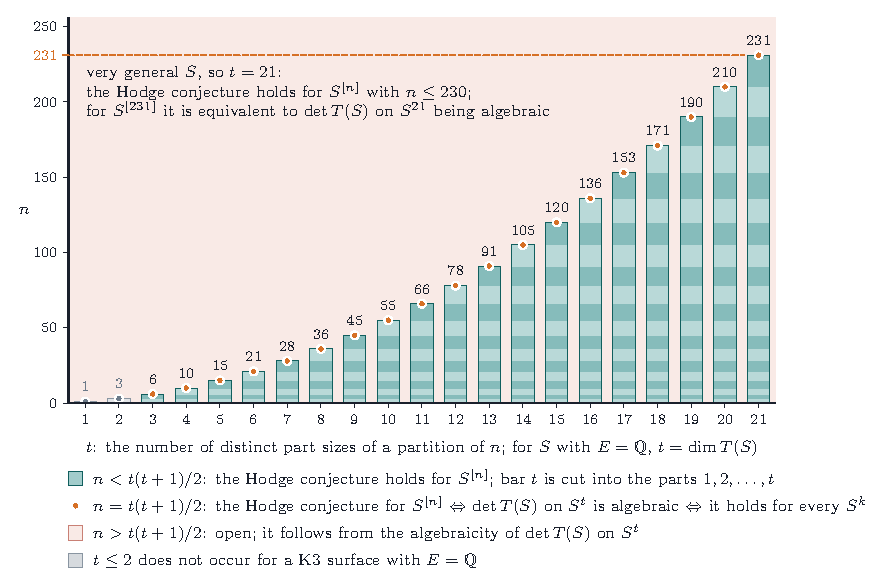
\includegraphics[width=\textwidth]{fig_k3threshold}
\caption{The threshold of \Cref{prop:k3powers}(ii). For $t=1,\dots,21$ the
bar rises to $t(t+1)/2$, the least $n$ that has a partition with $t$ distinct
part sizes, and is cut into the parts $1,2,\dots,t$ of the partition that
attains it. For a K3 surface $S$ with $E=\End_{\mathrm{Hdg}}(T(S))=\QQ$ and
$t=\dim T(S)$, which is at least $3$, the Hodge conjecture holds for
$S^{[n]}$ with $n$ below the bar; at its top it is equivalent to the
algebraicity of the class $\det T(S)$ on $S^{t}$ of \Cref{prop:orthpowers},
and to the Hodge conjecture for every power of $S$; above it, it follows
from that algebraicity. A very general $S$ has $t=21$: the
conjecture holds for $S^{[n]}$ with $n\le230$, and for $S^{[231]}$ it is
equivalent to the algebraicity of $\det T(S)$ on $S^{21}$, one of the
frontier cases of \textup{(F3$'$)} (\Cref{rem:f3primefrontier}).}
\label{fig:k3threshold}
\end{figure}

\begin{proposition}[Varieties of K3$^{[n]}$ type]\label{prop:k3ntype}
Let $X$ be a smooth projective hyperk\"ahler variety deformation equivalent
to the Hilbert scheme of $n\ge2$ points on a K3 surface, $q$ the
Beauville--Bogomolov form on $H^{2}=H^{2}(X,\QQ)$, $\NS=\NS(X)_{\QQ}$,
$T=\NS^{\perp}$ and $E=\End_{\mathrm{Hdg}}(T)$, a totally real field or a CM
field whose adjoint involution for $q$ is complex conjugation \cite{Zar83}.
Let $\mathrm{SH}(X)\subseteq H^{*}(X,\QQ)$ be the subalgebra generated by
$H^{2}$, and for $\varphi\in E$ with $\varphi^{*}=\varphi$ let
$c_{\varphi}=\sum_{i}t_{i}^{\vee}\cup\varphi(t_{i})\in H^{4}(X,\QQ)$, with
$(t_{i})$ a basis of $T$ and $(t_{i}^{\vee})$ its dual basis for $q$.
\begin{enumerate}[label=\textup{(\roman*)},leftmargin=2.6em,itemsep=2pt]
\item The Hodge classes of $\mathrm{SH}(X)$ are spanned by products of
  divisor classes and classes $c_{\varphi}$.
\item If $E$ is $\QQ$ or a CM field, every Hodge class of $\mathrm{SH}(X)$ is
  algebraic.
\item Let $n=2$. Then $\mathrm{SH}(X)=H^{*}(X,\QQ)$, with
  $b_{4}(X)=276=\dim\mathrm{Sym}^{2}H^{2}$, and $c_{2}(X)=\frac65q^{\vee}$,
  where $q^{\vee}\in\mathrm{Sym}^{2}H^{2}$ is dual to $q$. So the Hodge
  conjecture holds for $X$ when $E$ is $\QQ$ or a CM field. When $E$ is
  totally real of degree at least two, it holds for $X$ if and only if every
  element of $E$, acting on $T$ and by zero on $\NS$, is induced by an
  algebraic cycle on $X\times X$.
\end{enumerate}
This is a consequence of \cite{Mar24,CM13}; we make no claim of priority.
\end{proposition}

\begin{proof}
(i) Multiplication $\mathrm{Sym}^{k}H^{2}\to\mathrm{SH}^{2k}(X)$ is a
surjective morphism of polarisable Hodge structures, so by semisimplicity
every Hodge class of $\mathrm{SH}^{2k}(X)$ is the image of one of
$\mathrm{Sym}^{k}H^{2}=\bigoplus_{a+b=k}\mathrm{Sym}^{a}\NS\otimes
\mathrm{Sym}^{b}T$, whose Hodge classes are
$\mathrm{Sym}^{a}\NS\otimes(\mathrm{Sym}^{b}T)^{\Hdg}$. The isomorphism
$\End(T)\cong T\otimes T$ of the proof of \Cref{prop:k3powers}, now for $q$,
carries the adjoint to the exchange of the factors, so
$(\mathrm{Sym}^{2}T)^{\Hdg}$ consists of the tensors of the self-adjoint
$\varphi\in E$, whose images in $H^{4}$ are the $c_{\varphi}$. Over $\CC$ the
Hodge group of $T$ is a product of groups $\SO(T_{\sigma})$ on
$T_{\CC}=\bigoplus_{\sigma}T_{\sigma}$, with $\dim T_{\sigma}=\dim_{E}T\ge3$,
when $E$ is totally real, and of groups $\GL(W_{\sigma})$ on
$T_{\CC}=\bigoplus_{\sigma}(W_{\sigma}\oplus W_{\sigma}^{\vee})$ when $E$ is a
CM field \cite{Zar83}. By the first fundamental theorems
\cite[Chapter~5]{GW09}, the invariant polynomials of one vector of
$T_{\sigma}$, or of one vector of $W_{\sigma}$ and one of $W_{\sigma}^{\vee}$,
are generated by the quadratic form, or by the pairing: a determinant needs
$\dim T_{\sigma}$ distinct vectors. So $(\mathrm{Sym}^{b}T)^{\Hdg}\otimes\CC$
is spanned by products of elements of $(\mathrm{Sym}^{2}T)^{\Hdg}\otimes\CC$,
and the rational span of the products of classes $c_{\varphi}$, which has the
same complexification, is $(\mathrm{Sym}^{b}T)^{\Hdg}$.

(ii) Divisor classes are algebraic, so by (i) it suffices that every
$c_{\varphi}$ is. By \cite[Theorem~1.1]{CM13} the Lefschetz standard
conjecture holds for $X$, so the K\"unneth projectors and the inverse of the isomorphism
$L^{2n-2}\colon H^{2}\to H^{4n-2}$, $L$ the cup product with an ample class
$h$, are induced by algebraic cycles \cite{Kle68,Kle94}. Let $u\in E$ with
$u\bar u=1$, and $u=1$ if $E=\QQ$. The map $f_{u}=\id_{\NS}\oplus u$ is a
rational Hodge isometry of $H^{2}$, so by \cite[Theorem~1.1]{Mar24} there is
an algebraic class $Z_{u}$ on $X\times X$ (the diagonal if $u=1$) inducing on
$H^{2}$ a nonzero rational multiple of $f_{u}$: the class of the
correspondence $\tilde f$ of that theorem if it preserves degrees, and the
class of $\tilde f\circ(c_{2}(X)^{n-1}\cup\,\cdot\,)$ if it reverses them.
The class $Z_{u}$ may act in other degrees too; its K\"unneth component in
$H^{4n-2}(X)\otimes H^{2}(X)$ is algebraic and induces a nonzero multiple of
$f_{u}$ on $H^{2}$ and zero elsewhere. Applying $(L^{2n-2})^{-1}\otimes\id$
gives, up to a nonzero rational factor, the algebraic class
$\sum_{i}b_{i}\otimes f_{u}(a_{i})$, for a basis $(a_{i})$ of $H^{2}$ and
the dual basis $(b_{i})$ for $B(x,y)=\int_{X}xyh^{2n-2}$. Polarising the
relation $\int_{X}\alpha^{2n}=c_{X}q(\alpha)^{n}$ of Fujiki and Beauville
\cite{Bea83,Fuj87} gives
\[
  B(x,y)=\frac{c_{X}}{2n-1}\,q(h)^{n-2}\bigl(q(h)q(x,y)+2(n-1)q(x,h)q(y,h)\bigr),
\]
so $\NS$ and $T$ are orthogonal for $B$, and $B=\kappa q$ on $T$ with
$\kappa=c_{X}q(h)^{n-1}/(2n-1)\ne0$. With $(a_{i})$ adapted to
$\NS\oplus T$, the pull-back along the diagonal is
$\sum_{i}b_{i}\cup f_{u}(a_{i})=\nu+\kappa^{-1}c_{(u+\bar u)/2}$ with
$\nu\in\mathrm{Sym}^{2}\NS$ algebraic, because cup product on $H^{2}$ is
commutative and the exchange of factors turns $u$ into $\bar u$. So
$c_{(u+\bar u)/2}$ is algebraic. When $E$ is a CM field its elements of norm
one span it (proof of \Cref{prop:k3powers}(i)), so the $(u+\bar u)/2$ span
$E_{0}$, the self-adjoint part of $E$; when $E=\QQ$, $u=1$ suffices. So
every $c_{\varphi}$ is algebraic.

(iii) The variety $X$ has the Betti numbers of $S^{[2]}$, which by
\cite{dCM02} are those of $\mathrm{Sym}^{2}H^{*}(S)\oplus H^{*}(S)(-1)$:
$H^{\mathrm{odd}}(X)=0$ and $b_{4}(X)=253+1+22=276=\dim\mathrm{Sym}^{2}H^{2}$.
Here $c_{X}=3$, and the relation of Fujiki and Beauville gives
$\int_{X}abcd=q(a,b)q(c,d)+q(a,c)q(b,d)+q(a,d)q(b,c)$ for $a,b,c,d\in H^{2}$.
This form on $\mathrm{Sym}^{2}H^{2}$ is nondegenerate: in a $q$-orthogonal
basis $(e_{i})$ with $q(e_{i},e_{i})=d_{i}$, the $e_{i}e_{j}$ with $i<j$ are
orthogonal to each other and to the squares, with $\int_{X}(e_{i}e_{j})^{2}=
d_{i}d_{j}$, and on the squares the form has the matrix $D(J+2I)D$, with
$D=\mathrm{diag}(d_{i})$ and $J$ the matrix of ones, of determinant
$2^{22}\cdot25\prod_{i}d_{i}^{2}$. So
$\mathrm{Sym}^{2}H^{2}\to H^{4}$ is injective, hence bijective, and with
$H^{6}=h^{2}\cup H^{2}$ by the hard Lefschetz theorem,
$\mathrm{SH}(X)=H^{*}(X,\QQ)$. By \cite{Fuj87},
$\int_{X}c_{2}(X)xy=C\,q(x,y)$ for a constant $C$, and the Riemann--Roch
polynomial $\chi(L)=\binom{q(L)/2+3}{2}$ \cite{EGL01} gives $C=30$; the
Fujiki relation gives $\int_{X}q^{\vee}xy=25\,q(x,y)$, so
$c_{2}(X)=\frac65q^{\vee}$ by nondegeneracy. For $E=\QQ$ this makes
$c_{1}=q^{\vee}-q^{\vee}_{\NS}$ algebraic without \cite{CM13}, with
$q^{\vee}_{\NS}\in\mathrm{Sym}^{2}\NS$ the class dual to $q|_{\NS}$. With (i) and (ii) this proves the Hodge
conjecture for $X$ when $E$ is $\QQ$ or a CM field. Let $E$ be totally real
and $\varphi\in E$. If $\varphi\oplus0$ is induced by an algebraic cycle, the
computation of (ii) with $\varphi\oplus0$ in place of $f_{u}$ makes
$c_{\varphi}$ algebraic. Conversely, if $c_{\varphi}$ is algebraic, so is the
correspondence $x\mapsto(L^{2})^{-1}(c_{\varphi}\cup x)$. The Fujiki relation
gives $\int_{X}c_{\varphi}xy=\Tr(\varphi)q(x,y)+2q(\varphi x,y)$ for $x\in T$
and $y\in H^{2}$, and $B(z,y)=q(h)q(z,y)$ for $z\in T$, so that
correspondence acts on $T$ as $(\Tr(\varphi)+2\varphi)/q(h)$. The projector
onto $T$, the K\"unneth projector $\pi_{2}$ minus
$\sum_{j}n_{j}^{\vee}\otimes n_{j}$ over a basis $(n_{j})$ of $\NS$ and the
Hodge classes $n_{j}^{\vee}\in H^{6}$ dual to it, is algebraic by
\Cref{prop:f3prime}(iv); composing with it, $\varphi\oplus0$ is induced by an
algebraic cycle. By (i) the Hodge conjecture for $X$ is the algebraicity of
the $c_{\varphi}$, which proves the equivalence.
\end{proof}

For varieties of generalised Kummer type every Hodge class in the subalgebra
generated by $H^{2}$ is algebraic, whatever the field, and the Hodge
conjecture holds in dimension four \cite{FV25}. The preprint \cite{OG26}
announces, with \cite{Mar24}, that rational Hodge isometries between
varieties of the types K3$^{[a_{1}^{2}+1]}$ and K3$^{[a_{2}^{2}+1]}$ are
induced by algebraic cycles; it is not used here.

\begin{corollary}[Cubic fourfolds and their Fano varieties of lines]
\label{cor:fanolines}
Let $Y\subset\PP^{5}$ be a smooth cubic fourfold, $T(Y)\subset
H^{4}(Y,\QQ)$ the orthogonal complement of the Hodge classes,
$E(Y)=\End_{\mathrm{Hdg}}(T(Y))$, and $F=F(Y)$ the Fano variety of lines on
$Y$. The Hodge conjecture for $F$, the Hodge conjecture for $Y\times Y$, and
the statement that every element of $E(Y)$ acts on $T(Y)$ through an
algebraic cycle on $Y\times Y$ are equivalent. They hold when $E(Y)$ is $\QQ$
or a CM field, for instance when $Y$ is very general.
\end{corollary}

\begin{proof}
The Hodge conjecture holds for $Y$ \cite{Zuc77}, and also by
\Cref{prop:f3primesmall}, since $Y$ is covered by lines. So $H^{*}(Y,\QQ)$
is $T(Y)$ plus a space spanned by algebraic classes, on which the intersection
form is nondegenerate by the Hodge--Riemann relations, and as in the proof of
\Cref{prop:orthpowers} the part $\pi_{T}$ of the diagonal in
$T(Y)\otimes T(Y)$ is algebraic. The Hodge structure $T(Y)$ is of K3 type up
to a Tate twist and has no nonzero Hodge class, so $E(Y)$ is a field
\cite{Zar83}, and as in \Cref{prop:k3powers}(iii) the Hodge conjecture for
$Y\times Y$ is the third statement. By \cite{BD85}, $F$ is a hyperk\"ahler
fourfold of K3$^{[2]}$ type, and the universal line $P\subset F\times Y$
induces an isomorphism of Hodge structures $\alpha=P_{*}\colon
H^{4}(Y,\QQ)\to H^{2}(F,\QQ)$ up to a Tate twist. Both $T(Y)$ and $T(F)$
are the sums of the isotypic components that are not of Tate type, so
$\alpha(T(Y))=T(F)$ and $E(F)=\alpha E(Y)\alpha^{-1}$. Let $g$ be the
Pl\"ucker class on $F$ and $e=P^{t}_{*}\circ(g^{2}\cup\,\cdot\,)
\circ\alpha$, an algebraic correspondence that maps $T(Y)$ to itself, so that
$e|_{T(Y)}\in E(Y)$. For $0\ne\sigma\in H^{3,1}(Y)$,
$\int_{Y}e(\sigma)\bar\sigma=\int_{F}g^{2}\alpha(\sigma)\alpha(\bar\sigma)
=q(g)\,q(\alpha(\sigma),\alpha(\bar\sigma))\ne0$ by the Fujiki relation, since
$q(g)>0$ and $\alpha(\sigma)$ spans $H^{2,0}(F)$. So $e|_{T(Y)}$ is
invertible, its inverse is a polynomial in it and is algebraic, and the
inverse of $\alpha$ on $T(F)$,
which is $e^{-1}\circ P^{t}_{*}\circ(g^{2}\cup\,\cdot\,)$, is induced by an
algebraic cycle. Hence $\varphi\in E(Y)$ acts through an algebraic cycle on
$Y\times Y$ if and only if $\alpha\varphi\alpha^{-1}$ acts through one on
$F\times F$, and \Cref{prop:k3ntype}(iii) proves the equivalences and the
case where $E(Y)=E(F)$ is $\QQ$ or a CM field. A very general $Y$ has
$E(Y)=\QQ$.
\end{proof}

The class $\mathcal{A}$ of \Cref{prop:f3prime}(iii) is larger than the
closure properties recorded there show. Four further operations
preserve it, the last of them domination by correspondences, which brings in
the varieties whose motives are known to be built from those of abelian
varieties, and two classical families lie in it.

\begin{proposition}[More varieties of $\mathcal{A}$]\label{prop:aclosure}
Let $\mathcal{A}$ be as in \Cref{prop:f3prime}(iii).
\begin{enumerate}[label=\textup{(\roman*)},leftmargin=2.6em,itemsep=2pt]
\item If $Y\in\mathcal{A}$ and $Z\subset Y$ is a smooth closed subvariety
  with $Z\in\mathcal{A}$, then the blow-up $\mathrm{Bl}_{Z}Y$ lies in
  $\mathcal{A}$. If $Y\in\mathcal{A}$ and $V$ is a vector bundle on $Y$,
  then $\PP(V)\in\mathcal{A}$.
\item If $S\in\mathcal{A}$ is a surface, then the Hilbert scheme $S^{[n]}$
  lies in $\mathcal{A}$ for every $n\ge1$.
\item Every Fermat hypersurface
  $X^{r}_{m}=\{x_{0}^{m}+\dots+x_{r+1}^{m}=0\}\subset\PP^{r+1}$, $r\ge0$,
  $m\ge1$, lies in $\mathcal{A}$.
\item A K3 surface $S$ lies in $\mathcal{A}$ as soon as its Kuga--Satake
  correspondence is induced by an algebraic cycle, that is, as soon as some
  algebraic cycle $\Gamma$ on $S\times B$, with $B$ an abelian variety,
  induces a nonzero map $T(S)_{\QQ}\to H^{2}(B,\QQ)$.
\item If $H^{*}(X,\QQ)$ is the sum of the images of the $H^{*}(Y_{i},\QQ)$,
  with $Y_{i}\in\mathcal{A}$, under algebraic correspondences, then
  $X\in\mathcal{A}$; in particular $X\in\mathcal{A}$ when its Chow motive is
  a direct summand of a sum of Tate twists of motives of members of
  $\mathcal{A}$, for instance when it is of abelian type. So $\mathcal{A}$
  contains the $2n$-dimensional generalised Kummer varieties $K_{n}(A)$ of
  abelian surfaces $A$ \cite[Theorem~2.7, Corollary~2.8]{Xu15},
  \cite[Theorem~1.5]{FTV19}; the smooth projective moduli spaces of Gieseker
  stable (twisted) sheaves, or of $\sigma$-stable objects for a generic
  stability condition $\sigma$, on abelian surfaces and on K3 surfaces in
  $\mathcal{A}$ \cite[Theorem~0.1, Remark~2.1]{Bue20}; O'Grady's
  six-dimensional varieties $\widetilde K_{v}(A,H)$ obtained from moduli
  spaces of sheaves on an abelian surface $A$, with $v=2v_{0}$, $v_{0}$
  primitive, effective and of square $2$, and $H$ a $v$-generic polarisation
  \cite[Theorem~1.1]{Flo23}; the crepant resolutions of the ten-dimensional
  moduli spaces $M_{\sigma}(2v_{0})$ of $\sigma$-semistable objects, with
  $v_{0}$ primitive, $v_{0}^{2}=2$ and $\sigma$ $v_{0}$-generic, on abelian
  surfaces and on K3 surfaces in $\mathcal{A}$
  \cite[Theorem~1.3, Corollary~4.5]{FFZ21}; and the cubic fourfolds whose
  lattice of algebraic $2$-cycles has rank greater than $19$, with their Fano
  varieties of lines, the eightfolds of Lehn, Lehn, Sorger and van Straten of
  those containing no plane, and the tenfolds of Laza, Sacc\`a and Voisin of
  infinitely many Pfaffian cubic fourfolds \cite[Theorem~3.5 and its proof,
  Proposition~3.9, Theorem~4.2]{ABLP26}.
\end{enumerate}
Consequently \textup{(F3$'$)} holds on every smooth projective variety
obtained from abelian varieties, curves, Fermat hypersurfaces and K3 surfaces
as in \textup{(iv)} by products, surjective images, blow-ups along smooth
centres in $\mathcal{A}$, projective bundles and Hilbert schemes of points on
surfaces, and on every variety dominated by these as in \textup{(v)}.
\end{proposition}

\begin{proof}
(i) Let $c$ be the codimension of $Z$, $E=\PP(N_{Z/Y})$ the exceptional
divisor, $j\colon E\to\widetilde Y=\mathrm{Bl}_{Z}Y$ its inclusion,
$\rho\colon E\to Z$ and $\pi\colon\widetilde Y\to Y$ the projections and
$\xi=c_{1}(\cO_{E}(1))$. By the blow-up formula \cite[\S7.3.3]{Voi02},
\[
  H^{*}(\widetilde Y,\QQ)=\pi^{*}H^{*}(Y,\QQ)\oplus
  \bigoplus_{i=0}^{c-2}j_{*}\bigl(\xi^{i}\cup\rho^{*}H^{*}(Z,\QQ)\bigr).
\]
The first summand is the image of the transpose of the graph of $\pi$, and
the $i$-th of the others is the image of the algebraic cycle
$(\rho\times j)_{*}\xi^{i}$ on $Z\times\widetilde Y$. Composing with the
correspondences that exhibit $Y$ and $Z$ as members of $\mathcal{A}$, which is
allowed \cite[Chapter~16]{Ful98}, shows that $H^{*}(\widetilde Y,\QQ)$ is
spanned by classes $\Gamma_{*}y$ with $B$ abelian. For $\PP(V)$ the
projective bundle formula $H^{*}(\PP(V),\QQ)=\bigoplus_{i}\xi^{i}\cup
\pi^{*}H^{*}(Y,\QQ)$ \cite[\S7.3.3]{Voi02} does the same with the
algebraic cycles $\Gamma_{\pi}^{t}\cdot\mathrm{pr}^{*}\xi^{i}$.

(ii) By de Cataldo and Migliorini \cite{dCM02}, for every partition $\nu$ of
$n$ with $l(\nu)$ parts the incidence correspondence
$\Gamma_{\nu}\subset S^{(\nu)}\times S^{[n]}$ between the product
$S^{(\nu)}$ of symmetric products attached to $\nu$ and the Hilbert scheme
induces, after a Tate twist by $n-l(\nu)$, an isomorphism
$\bigoplus_{\nu}H^{*}(S^{(\nu)},\QQ)\to H^{*}(S^{[n]},\QQ)$. Let
$q_{\nu}\colon S^{l(\nu)}\to S^{(\nu)}$ be the quotient by the finite group
$G_{\nu}$. With rational coefficients the cycles and the cohomology of
$S^{(\nu)}$ are the $G_{\nu}$-invariants of those of $S^{l(\nu)}$
\cite[Example~1.7.6]{Ful98}, so $\Gamma_{\nu}$ pulls back to a cycle
$\widetilde\Gamma_{\nu}$ with rational coefficients on the smooth variety
$S^{l(\nu)}\times S^{[n]}$, whose action on $H^{*}(S^{l(\nu)},\QQ)$ is
$\Gamma_{\nu*}\circ q_{\nu*}$ up to a nonzero factor. As
$H^{*}(S^{(\nu)},\QQ)=q_{\nu*}H^{*}(S^{l(\nu)},\QQ)$, the $\nu$-th summand
is the image of $H^{*}(S^{l(\nu)},\QQ)$ under $\widetilde\Gamma_{\nu}$. Products of members of $\mathcal{A}$ lie in
$\mathcal{A}$, so $S^{[n]}\in\mathcal{A}$.

(iii) By induction on $r$, following the inductive structure of Shioda and
Katsura \cite{SK79}. For $r=0$, $X^{0}_{m}$ is a finite set of points, and
$X^{1}_{m}$ is a curve. Let $r\ge2$ and $r=a+b$ with $a,b\ge1$; fix
$\epsilon$ with $\epsilon^{m}=-1$ and put
\[
  \varphi\bigl((x),(y)\bigr)=\bigl(x_{0}y_{b+1}:\dots:x_{a}y_{b+1}:
  \epsilon x_{a+1}y_{0}:\dots:\epsilon x_{a+1}y_{b}\bigr),
\]
a rational map $X^{a}_{m}\times X^{b}_{m}\dashrightarrow\PP^{r+1}$; since
$\sum_{i\le a}x_{i}^{m}=-x_{a+1}^{m}$ and $\sum_{k\le b}y_{k}^{m}=-y_{b+1}^{m}$,
its image lies in $X^{r}_{m}$. It is defined by sections of
$\cO(1,1)$ whose common zero scheme is $\{x_{a+1}=0\}\times\{y_{b+1}=0\}$,
the product $Z\cong X^{a-1}_{m}\times X^{b-1}_{m}$ of two smooth
hyperplane sections, transversal because the Fermat hypersurfaces
are smooth. Blowing up that reduced scheme resolves the map, so $\varphi$
extends to a morphism $\widetilde\varphi\colon\mathrm{Bl}_{Z}(X^{a}_{m}\times
X^{b}_{m})\to X^{r}_{m}$. It is dominant: at a point $z$ of $X^{r}_{m}$ with
$\sum_{i\le a}z_{i}^{m}\ne0$ the preimages with $x_{a+1}=y_{b+1}=1$ are the
points $x_{i}=\lambda z_{i}$, $y_{k}=\lambda z_{a+1+k}/\epsilon$ with
$\lambda^{m}\sum_{i\le a}z_{i}^{m}=-1$, and both equations reduce to this one
because $\sum_{\text{all}}z_{i}^{m}=0$. So $\widetilde\varphi$ is surjective,
being proper. By induction $X^{a}_{m}$, $X^{b}_{m}$, $X^{a-1}_{m}$ and
$X^{b-1}_{m}$ lie in $\mathcal{A}$, hence so do their products, the blow-up
by (i) and $X^{r}_{m}$ as a surjective image; one may take $a=r-1$, $b=1$.

(iv) The transcendental part $T=T(S)_{\QQ}$ is an irreducible Hodge
structure, and $H^{*}(S,\QQ)=T\oplus T^{\perp}$ with $T^{\perp}$ spanned by
algebraic classes. Let $h$ be an ample class on $B$, $d=\dim B$, and let
$\phi=\Gamma^{t}_{*}\circ(\,\cdot\cup h^{d-2})\circ\Gamma_{*}$, an algebraic
correspondence from $S$ to itself and a morphism of Hodge structures. It
preserves $T$, because a morphism from the irreducible structure $T$ to the
algebraic part, which is of Tate type, vanishes; so $\phi|_{T}$ lies in the
field $\End_{\mathrm{Hdg}}(T)$. For $0\ne\sigma\in H^{2,0}(S)$,
$\Gamma_{*}\sigma\ne0$ because $T$ is irreducible and $\Gamma_{*}|_{T}\ne0$;
it is a class of type $(2,0)$ on $B$, hence primitive, and by the
Hodge--Riemann relations $\int_{S}\phi(\sigma)\,\bar\sigma=\int_{B}
\Gamma_{*}\sigma\,\overline{\Gamma_{*}\sigma}\,h^{d-2}\ne0$. So
$\phi|_{T}\ne0$, it is invertible, and $T\subseteq\Gamma^{t}_{*}H^{*}(B,\QQ)$.
With $T^{\perp}$ algebraic, $S\in\mathcal{A}$.

(v) If $H^{*}(X,\QQ)=\sum_{i}\Psi_{i*}H^{*}(Y_{i},\QQ)$ and each
$H^{*}(Y_{i},\QQ)$ is spanned by classes $\Gamma_{ij*}y$ with $B_{ij}$
abelian, then $H^{*}(X,\QQ)$ is spanned by the classes
$(\Psi_{i}\circ\Gamma_{ij})_{*}y$, and composites of algebraic
correspondences are algebraic \cite[Chapter~16]{Ful98}. If $h(X)$ is a
direct summand of $\bigoplus_{i}h(Y_{i})(n_{i})$, through $\alpha$ and
$\beta$ with $\beta\circ\alpha=\id$, then $\beta_{*}$ is surjective on
cohomology, and its components are the $\Psi_{i}$; a motive of abelian type
is such a summand with abelian varieties as the $Y_{i}$. The objects of the
tensor subcategory generated by $h(Y)$ are direct summands of sums of Tate
twists of the motives $h(Y^{k})$, since the dual of $h(Y)$ is a Tate twist of
$h(Y)$, and $Y^{k}\in\mathcal{A}$ when $Y\in\mathcal{A}$. The Chow motive of
$K_{n}(A)$ lies in the tensor subcategory generated by $h(A)$
\cite[Theorem~2.7, Corollary~2.8]{Xu15}, see also \cite[Theorem~1.5]{FTV19};
that of a moduli space as in (v) is a direct summand of a sum of Tate twists
of motives of powers of the surface \cite[Theorem~0.1]{Bue20}; those of the
varieties $\widetilde K_{v}(A,H)$ and of the ten-dimensional crepant
resolutions lie in the tensor subcategory generated by the motive of the
surface \cite[Theorem~1.1]{Flo23}, \cite[Corollary~4.5]{FFZ21}; and the cubic
fourfolds and hyperk\"ahler varieties of \cite{ABLP26} listed in (v) have
Chow motives of abelian type \cite[Theorem~3.5 and its proof,
Proposition~3.9, Theorem~4.2]{ABLP26}.

The last assertion is \Cref{prop:f3prime}(iii).
\end{proof}

The known cases of (iv) are recalled in \Cref{rem:mumfordks}; for the K3
surfaces among them whose powers are covered by \cite{Var22} the Hodge
conjecture itself holds on every power, which is stronger. What (iii) adds is
a family on which \textup{(F3$'$)} holds in every degree and dimension, while
the Hodge conjecture for Fermat hypersurfaces is proved in a range of degrees
and dimensions \cite{Shi79b}. Three recent preprints, if
correct, extend that range to every Fermat variety of degree less than $65$
other than $44$, $51$ and $52$ \cite{MMMV26}, to the Fermat fourfolds of
every odd degree at most $199$, by a computer-assisted proof \cite{Jum26},
and to the Fermat fourfold of degree $33$ \cite{FK26}; (iii) is new for the
degrees and dimensions outside these ranges. By (iii) and
\Cref{prop:f3prime}(i) the conjecture holds for $X^{r}_{m}$ as soon as it
holds for the powers of the Jacobian of the Fermat curve of degree $m$. The
inductive structure is Shioda and Katsura's, and the consequence for
\textup{(F3$'$)} is immediate; we claim no priority for it.

Item (v) collects consequences of published motivic results, and we claim no
priority for them either. For a generalised Kummer variety $K_{n}(A)$ it is
needed in general. The restriction from $A^{[n+1]}$, which lies in
$\mathcal{A}$ by (ii), reaches exactly the $A[n+1]$-invariant part of
$H^{*}(K_{n}(A),\QQ)$, since $A\times K_{n}(A)\to A^{[n+1]}$ is an \'etale
Galois cover with group $A[n+1]$. When $n+1$ is prime the rest is spanned by
the classes of the punctual Hilbert schemes at the points of $A[n+1]$, which
are algebraic, and (ii) suffices; when $n+1$ is composite the rest contains
transcendental classes, and \cite{Xu15,FTV19} are needed. These results
concern the varieties $K_{n}(A)$ themselves, not every variety of
generalised Kummer type; for products of varieties $K_{n}(A)$ the Hodge
conjecture itself is known \cite[Theorem~3.3]{Xu15}, and for the varieties
$\widetilde K_{v}(A,H)$ it holds on all self-products
\cite[Corollary~1.2]{Flo23}. If the
preprint \cite{Ped26} is correct, (v) also puts in $\mathcal{A}$ the tenfolds
of Laza, Sacc\`a and Voisin of every cubic fourfold in $\mathcal{A}$, whose
motives it makes direct summands of Tate twists of the motive of the fifth
power of the cubic fourfold. In low dimension the algebraicity results of
Bloch--Srinivas and Conte--Murre give more.

\begin{proposition}[Varieties whose zero-cycles are small]
\label{prop:f3primesmall}
Let $X$ be a smooth complex projective variety of dimension $n$ whose group
$\mathrm{CH}_{0}(X)_{\QQ}$ is supported on a closed subvariety of dimension at
most three. If $n\le5$, the Hodge conjecture holds for $X$, and so does
\textup{(F3$'$)}. This applies to every fourfold whose group of zero-cycles
is supported on a proper closed subset, in particular every uniruled
fourfold, and to every fivefold whose maximal rationally connected quotient
has dimension at most three, in particular every rationally connected
fivefold.
\end{proposition}

\begin{proof}
By Bloch and Srinivas \cite{BS83} every Hodge class of degree $4$ on $X$ is
algebraic. By \Cref{prop:f3prime}(iv) the Hodge classes of degree $0$, $2$,
$2n-2$ and $2n$ are algebraic, which settles $n\le4$. For $n=5$ the remaining
degree is $6=2n-4$, and cup product with $h$, for $h$ ample, is an isomorphism
$H^{4}(X,\QQ)\to H^{6}(X,\QQ)$ of Hodge structures up to a Tate twist by hard
Lefschetz, so every Hodge class of degree $6$ is $h$ times one of degree $4$.
A uniruled fourfold has $\mathrm{CH}_{0}$ supported on any ample divisor $D$,
because a rational curve through a point meets $D$ and any two points of
$\PP^{1}$ are rationally equivalent; this case is the theorem of Conte and
Murre \cite{CM78}. A proper closed subset of a fourfold has dimension at
most three.

Let $\phi\colon X\dashrightarrow R$ be the maximal rationally connected
fibration of Campana and of Koll\'ar, Miyaoka and Mori \cite{Cam92,KMM92}:
$R$, the maximal rationally connected quotient, is smooth and projective and
unique up to birational equivalence, and $\phi$ is dominant with connected
fibres, the general one rationally connected. Resolving its indeterminacy
\cite{Hir64} gives a smooth projective variety $\widetilde X$, a birational
morphism $\pi\colon\widetilde X\to X$, an isomorphism over the domain of
definition of $\phi$, and a surjective
morphism $\widetilde\phi\colon\widetilde X\to R$ whose general fibre is
smooth, by generic smoothness, and birational to a general fibre of $\phi$,
hence rationally connected. Suppose $\dim R\le3$, and let
$W\subset\widetilde X$ be a subvariety that $\widetilde\phi$ maps generically
finitely onto $R$, of degree $e$. Any two points of a general fibre $F$ are
joined by a rational curve, so every $x\in F$ satisfies $e[x]=[W\cap F]$ in
$\mathrm{CH}_{0}(\widetilde X)_{\QQ}$. The general fibres cover a dense open
subset of $\widetilde X$, and every zero-cycle is rationally equivalent to
one supported on a given dense open subset, so
$\mathrm{CH}_{0}(\widetilde X)_{\QQ}$ is supported on $W$ and
$\mathrm{CH}_{0}(X)_{\QQ}=\pi_{*}\mathrm{CH}_{0}(\widetilde X)_{\QQ}$ on
$\pi(W)$, of dimension $\dim R\le3$. A rationally connected fivefold is the
case where $R$ is a point.
\end{proof}

In degree four the hypothesis on zero-cycles can be relaxed to one on the
fibres of a map.

\begin{proposition}[Degree four along rationally connected fibrations]
\label{prop:f3primefibration}
Let $f\colon X\to Y$ be a surjective morphism of smooth complex projective
varieties whose general fibre is rationally connected. Then
$\Hdg^{2}(X)=\mathrm{Ab}^{2}(X)$ if and only if
$\Hdg^{2}(Y)=\mathrm{Ab}^{2}(Y)$, and every Hodge class of degree four on $X$
is algebraic if and only if every one on $Y$ is. Both properties are
therefore birational invariants of smooth projective varieties, and they hold
for $X$ exactly when they hold for a smooth projective model of its maximal
rationally connected quotient. Consequently \textup{(F3$'$)} holds for every
fourfold and every fivefold whose maximal rationally connected quotient is
birational to a variety $R$ with $\Hdg^{2}(R)=\mathrm{Ab}^{2}(R)$, for
instance a member of $\mathcal{A}$. With the Hodge conjecture for abelian
fourfolds \cite{Mar25a,Mar25b}, the Hodge conjecture holds for every fourfold
birational to an abelian fourfold, and for every fivefold admitting a
dominant rational map with rationally connected general fibre onto an
abelian fourfold.
\end{proposition}

\begin{proof}
Let $n=\dim X$ and $m=\dim Y$. Let $W$ be a component, dominating $Y$, of the
intersection of $X$ with a general linear space of codimension $n-m$, so that
$W\to Y$ is generically finite, of degree $e\ge1$; let
$i_{W}\colon\widetilde W\to X$ be a resolution of $W$ \cite{Hir64} and
$g=f\circ i_{W}$. The correspondence
$\Phi=\Gamma_{f}^{t}\circ\Gamma_{g}\circ\Gamma_{i_{W}}^{t}$ on $X\times X$
acts by $\Phi_{*}=f^{*}g_{*}i_{W}^{*}$ \cite[Chapter~16]{Ful98}. Let $\eta$ be
the generic point of $X$ and $K$ its field of functions. The restriction of
$\Phi^{t}$ to $\{\eta\}\times X$ is the zero-cycle $W_{f(\eta)}$, of degree
$e$, that $W$ cuts on the fibre of $X_{K}$ over the point $f(\eta)$, and that
of $[\Delta_{X}]$ is the point $\eta$ of the same fibre. Any two points of a
general fibre of $f$ are rationally equivalent, and the argument of Bloch and
Srinivas \cite{BS83} (a countable algebraically closed field of definition,
an embedding of an algebraic closure of $K$ into $\CC$, specialisation and a
norm) gives $e[\eta]=[W_{f(\eta)}]$ in $\mathrm{CH}_{0}(X_{K})_{\QQ}$. As
$\mathrm{CH}_{0}(X_{K})$ is the direct limit of the groups
$\mathrm{CH}^{n}(U\times X)$ over the dense open subsets $U\subseteq X$, the
cycle $e[\Delta_{X}]-\Phi^{t}$ vanishes on some $U\times X$, and by the
localisation sequence \cite[Chapter~1]{Ful98} it is supported on $D\times X$
for a divisor $D\supseteq X\smallsetminus U$. The diagonal is symmetric, so
$e[\Delta_{X}]-\Phi$ is supported on $X\times D$. Let $i\colon D'\to X$ be a
resolution of $D$. Each component of a cycle supported on $X\times D$ is, up
to a nonzero factor, the image of a subvariety of $X\times D'$ mapping
generically finitely onto it, so $e[\Delta_{X}]-\Phi=(\id\times i)_{*}\Psi$
for a cycle $\Psi$ with rational coefficients on $X\times D'$, and the
projection formula gives, for every $a\in H^{k}(X,\QQ)$,
\[
  e\,a=f^{*}g_{*}i_{W}^{*}a+i_{*}\Psi_{*}a,\qquad
  \Psi_{*}a\in H^{k-2}(D',\QQ).
\]

Let $a\in\Hdg^{2}(X)$. Then $g_{*}i_{W}^{*}a\in\Hdg^{2}(Y)$, and
$\Psi_{*}a$ is a Hodge class of degree two on $D'$, algebraic by the
Lefschetz theorem on $(1,1)$ classes. If $\Hdg^{2}(Y)=\mathrm{Ab}^{2}(Y)$,
then $f^{*}g_{*}i_{W}^{*}a\in\mathrm{Ab}^{2}(X)$, because composites of
algebraic correspondences are algebraic, and so $a\in\mathrm{Ab}^{2}(X)$; if
every Hodge class of degree four on $Y$ is algebraic, $a$ is algebraic.
Conversely, as in the proof of \Cref{prop:f3prime}(iii), for $h$ ample on
$X$ the correspondence $[\Gamma_{f}]\cdot\mathrm{pr}_{X}^{*}h^{n-m}$ sends
$f^{*}b$ to $c\,b$, with $c>0$ the degree of $h^{n-m}$ on a general fibre;
so $b\in\Hdg^{2}(Y)$ lies in $\mathrm{Ab}^{2}(Y)$, or is algebraic, as soon
as $f^{*}b$ does, or is.

A birational morphism is surjective with general fibre a point, and two
birational smooth projective varieties are dominated through birational
morphisms by a resolution of the closure of the graph \cite{Hir64}; so both
properties are birational invariants. The morphism
$\widetilde\phi\colon\widetilde X\to R$ of the proof of
\Cref{prop:f3primesmall}, from a variety birational to $X$ onto its maximal
rationally connected quotient, has rationally connected general fibre,
which gives the statement on $R$. For $n\le5$ the degrees $0$, $2$, $2n-2$
and $2n$ are settled by \Cref{prop:f3prime}(iv), and for $n=5$ cup product
with $h$ is an isomorphism $H^{4}(X,\QQ)\to H^{6}(X,\QQ)$ of Hodge structures
up to a Tate twist, so that $\Hdg^{3}(X)=h\cup\Hdg^{2}(X)$; members of
$\mathcal{A}$ satisfy \textup{(F3$'$)} by \Cref{prop:f3prime}(iii). An
abelian fourfold $B$ satisfies the Hodge conjecture \cite{Mar25a,Mar25b}. A
dominant rational map onto $B$ with rationally connected general fibre
becomes, after its indeterminacy is resolved, a morphism whose general fibre
is smooth and rationally connected, as in the proof of
\Cref{prop:f3primesmall}; so the fourfolds and fivefolds of the last
assertion have every Hodge class of degree four algebraic, and the other
degrees are settled as before.
\end{proof}

\Cref{prop:f3primefibration} reaches varieties that \Cref{prop:aclosure}
does not: conic bundles with singular fibres over members of $\mathcal{A}$ of
dimension three or four, and fourfolds and fivefolds birational to members
of $\mathcal{A}$ without being known to lie in $\mathcal{A}$. A projective
bundle over a member of $\mathcal{A}$ already lies in $\mathcal{A}$ by
\Cref{prop:aclosure}(i), and so, by \Cref{prop:aclosure}(v) and the
Leray--Hirsch theorem, does the source of a smooth morphism onto a member of
$\mathcal{A}$ on which algebraic classes restrict to a basis of the
cohomology of a fibre, such as a Severi--Brauer bundle.
\Cref{prop:f3primefibration} is the relative form of the argument of Bloch
and Srinivas, and we claim no priority for it.

\begin{remark}[Zero-cycles alone go no further]\label{rem:f3primesharp}
Hypotheses on zero-cycles cannot carry \textup{(F3$'$)} further without the
fourfolds. If $\mathrm{CH}_{0}(X)_{\QQ}$ is supported on a closed subset $Z$,
with resolution $j\colon Z'\to X$, the proof of \Cref{prop:f3primefibration},
with the closure in $X\times Z$ of a zero-cycle on $Z_{K}$ rationally
equivalent to the generic point in place of $\Phi^{t}$, gives a divisor with
resolution $i\colon D'\to X$ and cycles $\Phi$ on $Z'\times X$ and $\Psi$ on
$X\times D'$ with $a=\Phi_{*}j^{*}a+i_{*}\Psi_{*}a$ for every
$a\in H^{k}(X,\QQ)$, where $\Psi_{*}a$ has degree $k-2$; this is the
transpose of the decomposition of Bloch and Srinivas \cite{BS83}. When
$Z\ne X$ and $a$ has type $(n,0)$, $n=\dim X$, the first term vanishes, as
$\dim Z'<n$, and the second has no component of type $(n,0)$; so
$H^{n,0}(X)=0$. A uniruled fivefold has its zero-cycles
supported on an ample divisor, and for a fourfold $Y$ and
$b\in\Hdg^{2}(Y)$ the class $\mathrm{pr}^{*}b$ is a Hodge class on
$Y\times\PP^{1}$ with $b=\mathrm{pr}_{*}(\mathrm{pr}^{*}b\cup\eta)$, for
$\eta$ the class of $Y\times\{0\}$. So \textup{(F3$'$)}, and likewise the
Hodge conjecture, holds for every uniruled fivefold if and only if it holds
in degree four for every fourfold.

It also holds for every rational sixfold if and only if it holds for every
fourfold. A rational sixfold has its zero-cycles supported on a point, so
the proof of \Cref{prop:f3primesmall} settles every degree but six; and it
is the image under a birational morphism of a variety obtained from
$\PP^{6}$ by blow-ups along smooth centres \cite{Hir64}, on which, by the
blow-up formula \cite[\S7.3.3]{Voi02}, the Hodge classes of degree six are
images under algebraic correspondences of Hodge classes of degree at most
four on the centres, of dimension at most four, and lie in
$\mathrm{Ab}^{3}$, or are algebraic, when the fourfolds satisfy
\textup{(F3$'$)}, or the conjecture. Conversely, a fourfold $Y$
is birational to a hypersurface in $\PP^{5}$; place it in a hyperplane of
$\PP^{6}$, and let $\widetilde Y$ be its smooth strict transform under an
embedded resolution $M\to\PP^{6}$ \cite{Hir64}. On the rational sixfold
$X=\mathrm{Bl}_{\widetilde Y}M$, with exceptional divisor $j\colon E\to X$
and projection $\rho\colon E\to\widetilde Y$, the normal bundle of $E$ is
$\cO_{E}(-1)$, so $a=-\rho_{*}j^{*}j_{*}\rho^{*}a$ for
$a\in H^{4}(\widetilde Y,\QQ)$; this recovers $\Hdg^{2}(\widetilde Y)$ from
$\Hdg^{3}(X)$ through algebraic correspondences, and
\Cref{prop:f3primefibration} passes from $\widetilde Y$ to $Y$.

Among smooth hypersurfaces, ordered by dimension and degree, the first
family that these results do not cover is that of the sextic fourfolds:
those of dimension at most three are covered by \Cref{prop:f3prime}(iv),
the fourfolds of degree at most five are Fano, hence rationally connected
\cite{Cam92,KMM92}, and covered by \Cref{prop:f3primesmall}, while a sextic
fourfold has $h^{4,0}=1$, so that its zero-cycles are not supported on a
proper closed subset and it is its own maximal rationally connected
quotient; the Fermat sextic lies in $\mathcal{A}$ by
\Cref{prop:aclosure}(iii). For a smooth sextic fourfold $Y$ in a
hyperplane of $\PP^{6}$ no resolution is needed, and the rational sixfold
$\mathrm{Bl}_{Y}\PP^{6}$, with $h^{6,0}=0$, $h^{5,1}=1$, $h^{4,2}=426$ and
$h^{3,3}=1753$ by the blow-up formula \cite[\S7.3.3]{Voi02} and the Hodge
numbers $1$, $426$, $1752$ of $Y$, satisfies \textup{(F3$'$)} if and only if
$Y$ does. For the Hodge
conjecture these equivalences are folklore, and we claim no priority for
them.
\end{remark}

Surjective morphisms carry $\mathcal{A}$ to itself (\Cref{prop:f3prime}(iii)).
In degree four the morphism can be replaced by any dominant rational map,
which reaches some of these sextic fourfolds.

\begin{proposition}[Degree four along dominant rational maps]
\label{prop:f3primedominant}
Let $\varphi\colon Y\dashrightarrow X$ be a dominant rational map of smooth
complex projective varieties.
\begin{enumerate}[label=\textup{(\roman*)},leftmargin=2.6em,itemsep=2pt]
\item If $\Hdg^{2}(Y)=\mathrm{Ab}^{2}(Y)$, then
  $\Hdg^{2}(X)=\mathrm{Ab}^{2}(X)$; if every Hodge class of degree four on
  $Y$ is algebraic, so is every one on $X$.
\item \textup{(F3$'$)} holds on every fourfold and every fivefold that
  admits a dominant rational map from a variety $Y$ with
  $\Hdg^{2}(Y)=\mathrm{Ab}^{2}(Y)$, for instance from a member of
  $\mathcal{A}$. The Hodge conjecture holds on every fourfold that admits a
  dominant rational map from an abelian fourfold, such as a smooth
  projective model of the quotient of an abelian fourfold by a finite group,
  and on every fivefold that admits one from the product of an abelian
  fourfold and a projective space.
\end{enumerate}
\end{proposition}

\begin{proof}
(i) Let $\Gamma\subset Y\times X$ be the closure of the graph of $\varphi$
and $\widetilde Y\to\Gamma$ a resolution of singularities \cite{Hir64}. The
projections give a birational morphism $\widetilde Y\to Y$ and a morphism
$g\colon\widetilde Y\to X$, which is surjective, being proper and dominant.
Both properties are birational invariants (\Cref{prop:f3primefibration}),
so they hold for $\widetilde Y$. Let $x\in\Hdg^{2}(X)$, let $h$ be ample on
$\widetilde Y$ and $r=\dim\widetilde Y-\dim X$, and let
$\Psi=[\Gamma_{g}]\cdot\mathrm{pr}_{\widetilde Y}^{*}h^{r}$, so that
$\Psi_{*}g^{*}x=c\,x$ with $c>0$, as in the proof of
\Cref{prop:f3prime}(iii). The class $g^{*}x$ is a Hodge class of degree four
on $\widetilde Y$, hence a sum of classes $\Gamma_{j*}\gamma_{j}$ as in
\Cref{def:f3prime}, or algebraic. So $x=c^{-1}\sum_{j}(\Psi\circ
\Gamma_{j})_{*}\gamma_{j}$ lies in $\mathrm{Ab}^{2}(X)$, or $x$ is
algebraic, since composites of algebraic correspondences are algebraic
\cite[Chapter~16]{Ful98}.

(ii) On a fourfold or a fivefold the degrees other than four and six are
settled by \Cref{prop:f3prime}(iv), and the same argument, the Lefschetz
theorem on $(1,1)$ classes and hard Lefschetz, makes the Hodge classes of
those degrees algebraic; on a fivefold cup product with an ample class is an
isomorphism from $H^{4}$ onto $H^{6}$ of Hodge structures up to a Tate twist,
so degree six follows from degree four. Members of $\mathcal{A}$ satisfy
\textup{(F3$'$)} (\Cref{prop:f3prime}(iii)). An abelian fourfold $B$
satisfies the Hodge conjecture \cite{Mar25a,Mar25b}, and by the K\"unneth
formula a Hodge class of degree four on $B\times\PP^{k}$ is a sum of
pull-backs of Hodge classes of degrees four, two and zero on $B$ multiplied
by powers of the hyperplane class, so it is algebraic. A quotient $B/G$ by a
finite group is dominated by $B$, and so is every smooth projective model of
it.
\end{proof}

Lefschetz theory carries the two statements from a variety to its ample
complete intersections, outside the middle degree always and in the middle
degree for a very general member.

\begin{proposition}[Ample complete intersections]
\label{prop:f3primeample}
Let $X$ be a smooth complex projective variety of dimension $N$, $L$ an
ample line bundle on $X$, and $Y=Y_{c}\subset Y_{c-1}\subset\dots\subset
Y_{0}=X$ with each $Y_{j}$ a smooth divisor of $Y_{j-1}$ in the linear
system of $L^{m_{j}}|_{Y_{j-1}}$, $m_{j}\ge1$; put $r=\dim Y=N-c\ge1$ and
let $i\colon Y\to X$ be the inclusion.
\begin{enumerate}[label=\textup{(\roman*)},leftmargin=2.6em,itemsep=2pt]
\item If $2p\ne r$, every Hodge class of degree $2p$ on $Y$ is $i^{*}\alpha$
  for a Hodge class $\alpha$ of degree $2p$ on $X$. So if \textup{(F3$'$)}, or
  the Hodge conjecture, holds for $X$ in degree $2p$, it holds for $Y$ in
  degree $2p$; if $r$ is odd and it holds for $X$ in every degree, it holds
  for $Y$ in every degree.
\item Let $r$ be even, $c=1$ and $L^{m_{1}}$ very ample, and let
  $V\subset H^{r}(Y,\QQ)$ be the vanishing cohomology, the kernel of the
  Gysin map $i_{*}$. If $V$ is not of type $(r/2,r/2)$, then for a very
  general $Y$ in the linear system every Hodge class of degree $r$ on $Y$ is
  $i^{*}\alpha$ for a Hodge class $\alpha$ on $X$, and the conclusion of (i)
  holds in degree $r$ as well.
\end{enumerate}
So the Hodge conjecture holds for every smooth ample divisor of odd dimension
in $B\times\PP^{k}$, for $B$ an abelian variety of dimension at most five, and
for the very general member of every very ample linear system on an abelian
fivefold; and \textup{(F3$'$)} holds for every smooth ample divisor of odd
dimension in a member of $\mathcal{A}$.
\end{proposition}

\begin{proof}
(i) By the Lefschetz hyperplane theorem \cite[Chapter~1]{Voi03}, applied
to each $Y_{j}\subset Y_{j-1}$, the restriction $i^{*}\colon H^{k}(X,\QQ)\to
H^{k}(Y,\QQ)$ is an isomorphism for $k<r$ and injective for $k=r$. Let
$2p<r$. Then $i^{*}$ is an isomorphism of Hodge structures in degree $2p$,
so every Hodge class on $Y$ is $i^{*}$ of a Hodge class on $X$. Let $2p>r$.
The Gysin map $i_{*}\colon H^{2p}(Y,\QQ)\to H^{2p+2c}(X,\QQ)$ is Poincar\'e
dual to $i^{*}$ in degree $2r-2p<r$, hence an isomorphism, and
$i_{*}i^{*}$ is cup product with $[Y]=m_{1}\cdots m_{c}\,c_{1}(L)^{c}$. By the
hard Lefschetz theorem \cite[Chapter~6]{Voi02}, cup product with
$c_{1}(L)^{c}$ maps $H^{2p}(X,\QQ)$ onto $H^{2p+2c}(X,\QQ)$ when $2p\ge N-c$,
so $i^{*}$ is onto in degree $2p$. A surjective morphism of polarisable
Hodge structures has a section that is a morphism of Hodge structures, so
again every Hodge class on $Y$ is $i^{*}$ of a Hodge class on $X$. The
restriction $i^{*}$ is induced by the transpose of the graph of $i$, so it
carries $\mathrm{Ab}^{p}(X)$ into $\mathrm{Ab}^{p}(Y)$ and algebraic classes
to algebraic classes, which gives the rest of (i).

(ii) The projection formula shows that $V$ is the orthogonal complement of
$i^{*}H^{r}(X,\QQ)$ for the intersection form, and
$H^{r}(Y,\QQ)=i^{*}H^{r}(X,\QQ)\oplus V$ as Hodge structures
\cite[Chapter~2]{Voi03}; the Hodge classes in the first summand are the
$i^{*}\alpha$ with $\alpha$ a Hodge class on $X$. Over the open set $U$ of
the linear system parametrising smooth members, $V$ is a local system, and
its monodromy group $\Gamma$ acts irreducibly \cite[Chapter~3]{Voi03}. For
each class $v$ of the lattice of $V$ at a point of the universal cover of
$U$, the set where the flat continuation of $v$ is of Hodge type is a closed
analytic subset, either everything or nowhere dense; so at a very general
point the Hodge classes of $V$ are those whose continuation is of Hodge type
everywhere. They form a subspace $W$ stable under $\Gamma$, hence $W=0$ or
$W=V$, and $W=V$ would make $V$ of type $(r/2,r/2)$. So $W=0$.

For the consequences, $B\times\PP^{k}$ satisfies the Hodge conjecture by the
K\"unneth formula, since $B$ does \cite{Mar25a,Mar25b,MZ99}. For a very ample
divisor $Y$ of an abelian fivefold $B$, $r=4$, and $V$ is not of type $(2,2)$:
$h^{4,0}(Y)=h^{0}(K_{Y})=h^{0}(Y,\cO_{Y}(Y))=h^{0}(B,\cO_{B}(Y))+4$, by the
sequence $0\to\cO_{B}\to\cO_{B}(Y)\to\cO_{Y}(Y)\to0$ and $h^{1}(\cO_{B}(Y))=0$,
exceeds $h^{4,0}(B)=5$ because $h^{0}(\cO_{B}(Y))\ge2$, so $V$ has a nonzero
part of type $(4,0)$. Members of $\mathcal{A}$ satisfy \textup{(F3$'$)} by
\Cref{prop:f3prime}(iii).
\end{proof}

For the Hodge conjecture these transfers are classical, and we claim no
priority. What they add to \textup{(F3$'$)} is a large class outside
$\mathcal{A}$: the vanishing cohomology of an ample divisor of odd dimension
is not reached from abelian varieties in general, yet it carries no Hodge
class in even degree, since its only degree is the odd middle one.

A hypersurface of Delsarte type is defined by as many monomials as
variables. Shioda observed that such a surface is dominated by a Fermat
surface \cite{Shi86}; the same monomial substitution works in every
dimension, and with \Cref{prop:f3primedominant} it gives the following.

\begin{proposition}[Delsarte fourfolds]\label{prop:delsarte}
Let $A=(a_{ij})_{0\le i,j\le r+1}$ be an invertible matrix of non-negative
integers whose rows all sum to $m\ge2$, let $F_{A}=\sum_{i}\prod_{j}
x_{j}^{a_{ij}}$, suppose that $X_{A}=\{F_{A}=0\}\subset\PP^{r+1}$ is smooth,
and let $d$ be a positive integer with $dA^{-1}$ integral, such as
$|\det A|$.
\begin{enumerate}[label=\textup{(\roman*)},leftmargin=2.6em,itemsep=2pt]
\item There is a dominant rational map from the Fermat hypersurface
  $X^{r}_{d}$ onto $X_{A}$, given by monomials.
\item $\Hdg^{2}(X_{A})=\mathrm{Ab}^{2}(X_{A})$. For $r=4$, $X_{A}$
  satisfies \textup{(F3$'$)}, and it satisfies the Hodge conjecture if
  $X^{4}_{d}$ does.
\item If $m\ge3$ and $F_{A}$ is a sum, in disjoint sets of variables, of
  terms $x^{m}$, chains $x_{1}^{m-1}x_{2}+\dots+x_{k-1}^{m-1}x_{k}+x_{k}^{m}$
  and loops $x_{1}^{m-1}x_{2}+\dots+x_{k-1}^{m-1}x_{k}+x_{k}^{m-1}x_{1}$
  with $k\ge2$, then $A$ is invertible and $X_{A}$ is smooth. For $r=4$ and
  $m=6$ these polynomials have $29$ shapes up to a renumbering of the
  variables, the Fermat sextic being one; each defines a smooth sextic
  fourfold, with $h^{4,0}=1$, $h^{3,1}=426$ and primitive $h^{2,2}$ equal
  to $1751$. The least $d$ is $6$ for the Fermat sextic, $24$ or $30$ for
  six others, those whose terms other than $x^{m}$ are all loops of length
  two or all chains of length two, at least $120$ for the remaining
  twenty-two, and $5^{6}-1=15624$ for the loop
  $x_{0}^{5}x_{1}+x_{1}^{5}x_{2}+\dots+x_{5}^{5}x_{0}$.
\end{enumerate}
\end{proposition}

\begin{proof}
(i) The matrix $dA^{-1}$ is integral for $d=|\det A|$, by the formula
for the inverse through the adjugate. Let $B=dA^{-1}$. From
$A\mathbf{1}=m\mathbf{1}$, with $\mathbf{1}$ the vector of ones,
$B\mathbf{1}=(d/m)\mathbf{1}$, so the rows of the integral matrix $B$ all
sum to the integer $d/m$, and $AB=d\cdot I$. Choose $c\ge0$
with every $b_{jk}+c\ge0$ and let $\psi(y)_{j}=\prod_{k}y_{k}^{b_{jk}+c}$;
the coordinates of $\psi$ are monomials of the same degree, so $\psi$ is a
rational map $\PP^{r+1}\dashrightarrow\PP^{r+1}$, and
\[
  F_{A}(\psi(y))=\sum_{i}\prod_{k}y_{k}^{\sum_{j}a_{ij}(b_{jk}+c)}
  =(y_{0}\cdots y_{r+1})^{cm}\sum_{i}y_{i}^{d}.
\]
On the torus $T$ of points with all coordinates nonzero, $\psi$ is induced
by the homomorphism $y\mapsto(\prod_{k}y_{k}^{b_{jk}})_{j}$ of
$\mathbb{G}_{m}^{r+2}$, which is surjective because $\det B\ne0$. So every
$z\in X_{A}\cap T$ is $\psi(y)$ for some $y\in T$, and the identity puts $y$
on $X^{r}_{d}$. A smooth hypersurface of degree at least two and positive
dimension is irreducible, so it is not contained in a coordinate hyperplane,
and $X_{A}\cap T$ and $X^{r}_{d}\cap T$ are dense. Hence $\psi$ restricts to
a dominant rational map $X^{r}_{d}\dashrightarrow X_{A}$.

(ii) $X^{r}_{d}$ lies in $\mathcal{A}$ by \Cref{prop:aclosure}(iii), so (i)
and \Cref{prop:f3primedominant} give both assertions, the degrees other than
four being settled as in the proof of \Cref{prop:f3primedominant}(ii).

(iii) The exponent matrix is block diagonal, with blocks $m$,
$(m-1)I+N+E$ for a chain, $N$ the nilpotent shift and $E$ the matrix whose
only nonzero entry is a $1$ in the last diagonal place, and $(m-1)I+P$ for a
loop, $P$ the cyclic shift; their determinants are $m$, $m(m-1)^{k-1}$ and
$(m-1)^{k}-(-1)^{k}$, which are nonzero. The partial derivatives of a sum in
disjoint sets of variables are those of the summands, so it suffices that
the partials of each summand vanish together only at $0$. For $x^{m}$ this
is clear. For a chain, $\partial F/\partial x_{1}=(m-1)x_{1}^{m-2}x_{2}$
vanishes only if $x_{1}=0$ or $x_{2}=0$, and if $x_{2}=0$ then
$\partial F/\partial x_{2}=x_{1}^{m-1}$; so $x_{1}=0$, the same argument
applies to $x_{2},\dots,x_{k-1}$, and then $\partial F/\partial
x_{k}=mx_{k}^{m-1}$ gives $x_{k}=0$. For a loop, $\partial F/\partial
x_{j}=(m-1)x_{j}^{m-2}x_{j+1}+x_{j-1}^{m-1}$, indices modulo $k$. If one
coordinate vanishes, so does the one before it, hence all of them; if none
vanishes, the product of the relations $x_{j-1}^{m-1}=-(m-1)x_{j}^{m-2}
x_{j+1}$ gives $\prod_{j}x_{j}^{m-1}=(1-m)^{k}\prod_{j}x_{j}^{m-1}$, which
is impossible because $|1-m|\ge2$. The number of shapes, drawn in \Cref{fig:delsarte}, is the
coefficient of $t^{6}$ in $(1-t)^{-1}\prod_{k\ge2}(1-t^{k})^{-2}$, which is $29$, and
the least $d$ is the least common multiple of the orders of the cyclic groups
attached to the terms in the proof of \Cref{cor:delsarteall}(iii): $6$ for
$x^{6}$, $6\cdot5^{k-1}$ for a chain and $5^{k}-(-1)^{k}$ for a loop of length
$k$; so $24$ or $30$ when the terms other than $x^{6}$ are all loops or all
chains of length two, and at least $\operatorname{lcm}(24,30)=120$, $5^{3}+1$
or $6\cdot5^{2}$ when both kinds of length two, or a loop or chain of length at
least three, occur. The
Hodge numbers are those of every smooth sextic fourfold, read off from the
Jacobian ring \cite[Chapter~6]{Voi03}.
\end{proof}

\begin{figure}[tbp]
\centering
  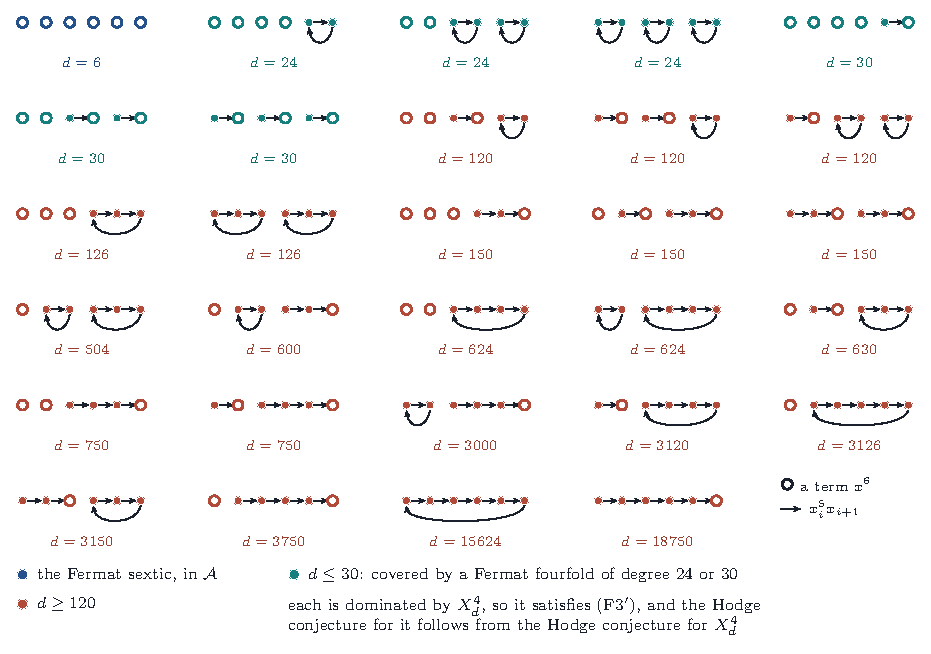
\includegraphics[width=\textwidth]{fig_delsarte}
\caption{The $29$ smooth sextic fourfolds of \Cref{prop:delsarte}(iii), up
to a renumbering of the variables. Each is drawn on its six variables: an
arrow from $x_{i}$ to $x_{j}$ is a term $x_{i}^{5}x_{j}$, and a ring is a
term $x^{6}$, so a chain is a path of arrows ending at a ring and a loop is
a cycle of arrows. Under each is the least $d$ with $dA^{-1}$ integral, the
degree of the Fermat fourfold that covers it. All of them satisfy
\textup{(F3$'$)}.}
\label{fig:delsarte}
\end{figure}

A sextic fourfold has $h^{4,0}=1$, so no hypothesis on zero-cycles or on
rationally connected fibrations reaches it (\Cref{rem:f3primesharp}), and
among the smooth sextic fourfolds only the Fermat one is covered by
\Cref{prop:aclosure}. The Delsarte sextics are finitely many
up to isomorphism, since the torus rescales the coefficients of a Delsarte
polynomial to $1$, so they are isolated points in the $426$-dimensional
moduli of smooth sextic fourfolds: \Cref{prop:delsarte} adds points, not a
family. By \Cref{prop:delsarte}(ii) the Hodge conjecture for a Delsarte
fourfold follows from that for one Fermat fourfold. For six of the sextic
shapes that Fermat fourfold has degree $24$ or $30$, inside the range claimed
in the preprint \cite{MMMV26}, so if it is correct the Hodge conjecture
itself holds on these six; for the others the degree ranges from $120$ to
$18750$, and from $120$ to $3750$ with the lattice degree of
\Cref{cor:delsarteall}, beyond every known or claimed range
\cite{Shi79b,MMMV26,Jum26}.
The monomial cover is Shioda's, and we claim no priority for it.

\Cref{prop:delsarte} uses the covering map only in degree four, where
algebraicity modulo abelian varieties descends along every dominant rational
map. In higher degrees a birational modification can add classes, so the
boundary of a compactification has to be controlled. For a hypersurface of a
torus defined by affinely independent monomials the boundary is again of the
same kind, and the whole cohomology can be traced back to Fermat varieties
of a single degree. We use toric varieties as in \cite{CLS11}: a torus $T$
with character lattice $M$ and cocharacter lattice $N$, a fan $\Sigma$ in
$N_{\RR}$ and its toric variety $Y_{\Sigma}$, and for a cone
$\tau\in\Sigma$ the orbit $O(\tau)$, whose character lattice is
$\tau^{\perp}\cap M$, and its closure $V(\tau)$, the toric variety of the
fan formed by the images of the cones containing $\tau$ in
$N_{\RR}/\RR\tau$ \cite[Chapter~3]{CLS11}; for a ray $\rho$ we write
$D_{\rho}=V(\rho)$. In what follows varieties need not be connected: a
smooth projective variety lies in $\mathcal{A}$ when each of its connected
components does, and the closure properties of \Cref{prop:f3prime}(iii) and
\Cref{prop:aclosure} hold component by component.

\begin{definition}[Simplex type]\label{def:simplextype}
Let $T$ be a torus of dimension $n$ with character lattice $M$. A Laurent
polynomial $f=\sum_{i=0}^{k}c_{i}\chi^{u_{i}}$ on $T$ is of \emph{simplex
type} if every $c_{i}$ is nonzero and $u_{0},\dots,u_{k}\in M$ are affinely
independent. Let $L'\subseteq M$ be the lattice spanned by the
$u_{i}-u_{0}$, $L$ its saturation, the set of $x\in M$ with a nonzero
multiple in $L'$, and $e(f)$ the exponent of the finite group $L/L'$; put
$V_{f}=\{f=0\}\subseteq T$. A fan $\Sigma$ in $N_{\RR}$ is \emph{adapted} to
$f$ if for every cone $\sigma\in\Sigma$ there is an index $i_{\sigma}$ with
$\langle u_{i_{\sigma}},v\rangle\le\langle u_{j},v\rangle$ for all $j$ and
all $v\in\sigma$, that is, if every cone of $\Sigma$ lies in a cone of the
normal fan of the simplex spanned by the $u_{i}$. For a cone $\tau$ of an
adapted fan let $I_{\tau}$ be the set of indices $i$ with
$\langle u_{i},v\rangle=\min_{j}\langle u_{j},v\rangle$ for every
$v\in\tau$, fix $i_{\tau}\in I_{\tau}$, and let
$f_{\tau}=\sum_{i\in I_{\tau}}c_{i}\chi^{u_{i}-u_{i_{\tau}}}$, a Laurent
polynomial of simplex type on the torus $O(\tau)$, since its exponents lie
in $\tau^{\perp}\cap M$.
\end{definition}

The compactification is Khovanskii's \cite{Kho77}; for a simplex the proof
is short, and we give it.

\begin{lemma}[The compactification]\label{lem:simplexchart}
Let $f$ be of simplex type on $T$, let $\Sigma$ be a smooth fan adapted to
$f$, and let $Z$ be the closure of $V_{f}$ in $Y_{\Sigma}$.
\begin{enumerate}[label=\textup{(\roman*)},leftmargin=2.6em,itemsep=2pt]
\item $V_{f}$ is empty if $k=0$. If $k\ge1$, it is a finite \'etale cover,
  of degree $[L:L']$, of the product of a torus of dimension $n-k$ and the
  complement of $k+1$ hyperplanes in general position in $\PP^{k-1}$; in
  particular it is smooth.
\item $Z$ is smooth, and for every $\tau\in\Sigma$, $Z\cap O(\tau)=V_{f_{\tau}}$
  and $Z$ meets $V(\tau)$ transversally: $Z\cap V(\tau)$ is empty or smooth of
  codimension $\dim\tau$ in $Z$, and it is the closure of $V_{f_{\tau}}$ in
  $V(\tau)$. So the divisors $Z\cap D_{\rho}$ of $Z$ are smooth and cross
  normally, and $Z\cap D_{\rho}$ is empty when $I_{\rho}$ has one element.
\item The fan of $V(\tau)$ is smooth and adapted to $f_{\tau}$.
\end{enumerate}
\end{lemma}

\begin{proof}
(i) If $k=0$, $f$ is a monomial and has no zero on $T$. Let $k\ge1$, choose a
complement $C$ of the saturated lattice $L$ in $M$ and a basis
$b_{k+1},\dots,b_{n}$ of $C$. The characters $u_{1}-u_{0},\dots,u_{k}-u_{0},
b_{k+1},\dots,b_{n}$ span a sublattice of index $[L:L']$ in $M$, so the map
$T\to(\CC^{\times})^{n}$ that they define is an isogeny of that degree. The
function $\chi^{-u_{0}}f$ is the pull-back of $c_{0}+c_{1}z_{1}+\dots+c_{k}
z_{k}$, so $V_{f}$ is the full preimage of the product of
$(\CC^{\times})^{n-k}$ and the set $H$ of points of $(\CC^{\times})^{k}$ with
$c_{0}+\sum_{i}c_{i}z_{i}=0$. The projective closure of this affine hyperplane is a hyperplane
$\PP^{k-1}$ of $\PP^{k}$, with homogeneous coordinates $w_{0},\dots,w_{k}$,
on which the $k+1$ linear forms $w_{i}$ satisfy the single relation
$\sum_{i}c_{i}w_{i}=0$, with every $c_{i}\ne0$; so any $k$ of them are
independent, the hyperplanes $\{w_{i}=0\}$ of $\PP^{k-1}$ are in general
position, and $H$ is their complement.

(ii) Let $\sigma\in\Sigma$, spanned by part $v_{1},\dots,v_{s}$ of a basis
$v_{1},\dots,v_{n}$ of $N$, let $w_{1},\dots,w_{n}$ be the dual basis of $M$,
and let $t_{j}=\chi^{w_{j}}$, the coordinates of
$U_{\sigma}\cong\CC^{s}\times(\CC^{\times})^{n-s}$. Put $i=i_{\sigma}$. Every
$u_{j}-u_{i}$ lies in the dual cone of $\sigma$, so
$g=\chi^{-u_{i}}f=\sum_{j}c_{j}\chi^{u_{j}-u_{i}}$ is a regular function on
$U_{\sigma}$, and $Z\cap U_{\sigma}\subseteq\{g=0\}$. A face $\tau$ of
$\sigma$ is spanned by the $v_{j}$ with $j$ in a subset $J$, and $O(\tau)$ is
the locus where exactly the $t_{j}$ with $j\in J$ vanish. A character
$\chi^{x}$ regular on $U_{\sigma}$ restricts to $O(\tau)$ as $\chi^{x}$ if
$x\in\tau^{\perp}$ and as $0$ otherwise \cite[Chapter~3]{CLS11}; since
$\langle u_{j}-u_{i},v\rangle\ge0$ on $\sigma$, $u_{j}-u_{i}\in\tau^{\perp}$
exactly when $j\in I_{\tau}$. So $h=g|_{O(\tau)}$ is
$\chi^{u_{i_{\tau}}-u_{i}}f_{\tau}$, a unit times $f_{\tau}$. Let $p\in
O(\tau)$ with $h(p)=0$ and put $a_{j}=c_{j}\chi^{u_{j}-u_{i}}(p)$ for $j\in
I_{\tau}$. The derivative of $h$ at $p$ along the one-parameter subgroup of
$O(\tau)$ given by $y$ in its cocharacter lattice is $\sum_{j}a_{j}\langle
u_{j}-u_{i},y\rangle$. If all of these vanished, then, with
$\sum_{j}a_{j}=h(p)=0$, the vector $\sum_{j}a_{j}(1,u_{j}-u_{i})$ of
$\CC\oplus(\tau^{\perp}\cap M)\otimes\CC$ would be zero, as the cocharacter
lattice of $O(\tau)$ is dual to $\tau^{\perp}\cap M$; affine independence
would give every $a_{j}=0$, which is impossible at a point of the torus
$O(\tau)$. So $dh(p)\ne0$. Hence $\{g=0\}$ is smooth at $p$ and transversal
to $O(\tau)$ and to every $\{t_{j}=0,\ j\in J'\}$ with $J'\subseteq J$, whose
tangent space at $p$ contains that of $O(\tau)$. No component of $\{g=0\}$
lies in a divisor $\{t_{j}=0\}$, since $g$ restricted to the orbit of the
ray of $v_{j}$ is a unit times a nonzero Laurent polynomial; so every
component meets $T$, where $\{g=0\}$ is $V_{f}$, and
$\{g=0\}=Z\cap U_{\sigma}$. This shows that $Z$ is smooth, that
$Z\cap O(\tau)=V_{f_{\tau}}$ and that $Z\cap V(\tau)$ is smooth of
codimension $\dim\tau$. As $Z\cap O(\tau')$ has codimension at least
$\dim\tau'$ in $Z$ for every cone $\tau'\supsetneq\tau$, no component of
$Z\cap V(\tau)$ lies in the smaller orbits, and $Z\cap V(\tau)$ is the
closure of $V_{f_{\tau}}$. If $I_{\rho}$ has one element, $f_{\rho}$ is a
nonzero constant.

(iii) The fan of $V(\tau)$ is smooth because $\Sigma$ is. Let $\sigma\supseteq
\tau$. The index $i_{\sigma}$ attains the minimum on $\sigma$, hence on
$\tau$, so $i_{\sigma}\in I_{\tau}$, and for $j\in I_{\tau}$ and $v\in\sigma$,
$\langle u_{i_{\sigma}}-u_{i_{\tau}},v\rangle\le\langle
u_{j}-u_{i_{\tau}},v\rangle$. Both sides depend only on the image of $v$ in
$N_{\RR}/\RR\tau$, because the exponents of $f_{\tau}$ lie in $\tau^{\perp}$;
so the image of $\sigma$ satisfies the condition of adaptedness for
$f_{\tau}$.
\end{proof}

\begin{lemma}[Cohomology across a toric modification]\label{lem:toricmod}
Let $f$ be of simplex type on $T$, let $\Sigma_{1}$ and $\Sigma_{0}$ be
smooth projective fans adapted to $f$, with $\Sigma_{1}$ refining
$\Sigma_{0}$, let $\varphi\colon Y_{1}=Y_{\Sigma_{1}}\to Y_{0}=Y_{\Sigma_{0}}$
be the toric morphism, and let $Z_{1}$ and $Z_{0}$ be the closures of
$V_{f}$. For each ray $\rho$ of $\Sigma_{1}$ that is not a ray of
$\Sigma_{0}$ let $E_{\rho}=Z_{1}\cap D_{\rho}$, with inclusion $i_{\rho}$.
Then the kernel of $\varphi_{*}\colon H^{k}(Z_{1},\QQ)\to H^{k}(Z_{0},\QQ)$ is
contained in $\sum_{\rho}i_{\rho*}H^{k-2}(E_{\rho},\QQ)$, and
\[
  H^{k}(Z_{1},\QQ)=\varphi^{*}H^{k}(Z_{0},\QQ)
  +\sum_{\rho}i_{\rho*}H^{k-2}(E_{\rho},\QQ).
\]
\end{lemma}

\begin{proof}
Let $W\subseteq Y_{0}$ be the union of the open sets $U_{\tau}$ with
$\tau\in\Sigma_{0}\cap\Sigma_{1}$. A cone of $\Sigma_{1}$ contained in such a
$\tau$ is a face of it, since two cones of a fan meet in a common face; so
$\varphi^{-1}(U_{\tau})=U_{\tau}$, and $\varphi$ is an isomorphism over $W$. A
cone of $\Sigma_{1}$ whose rays are all rays of $\Sigma_{0}$ lies in a cone
$\tau_{0}$ of $\Sigma_{0}$, its rays are rays of $\tau_{0}$, and $\tau_{0}$
is simplicial, so it is a face of $\tau_{0}$ and lies in $\Sigma_{0}$. Hence
$Y_{1}\smallsetminus\varphi^{-1}(W)$ is the union of the orbits of the cones
with a ray not in $\Sigma_{0}$, that is, of the divisors $D_{\rho}$ of those
rays. So $U_{1}=Z_{1}\smallsetminus\bigcup_{\rho}E_{\rho}$ is the closure of
$V_{f}$ in $\varphi^{-1}(W)$, and $\varphi$ maps it isomorphically onto
$U_{0}=Z_{0}\cap W$, with $U_{1}=Z_{1}\cap\varphi^{-1}(U_{0})$. The morphism
$Z_{1}\to Z_{0}$ is birational on each component, so $\varphi_{*}\varphi^{*}
=\id$ by the projection formula, and every class is $\varphi^{*}\varphi_{*}a$
plus a class in the kernel of $\varphi_{*}$. Let $\varphi_{*}b=0$.
Push-forward along a proper map commutes with restriction to an open set and
its preimage, so $b|_{U_{1}}=(\varphi|_{U_{1}})^{*}\bigl((\varphi_{*}b)|_{U_{0}}
\bigr)=0$. By \Cref{lem:simplexchart}(ii), $\bigcup_{\rho}E_{\rho}$ is a
divisor with normal crossings and smooth components in the smooth projective
variety $Z_{1}$, and by Deligne \cite[\S3.2]{Del71} the weight spectral
sequence of its complement $U_{1}$ degenerates at $E_{2}$; its term
$E_{2}^{0,k}$, the cokernel of the Gysin map
$\bigoplus_{\rho}H^{k-2}(E_{\rho},\QQ)\to H^{k}(Z_{1},\QQ)$, is the image of
$H^{k}(Z_{1},\QQ)$ in $H^{k}(U_{1},\QQ)$. So $b$ lies in the image of the
Gysin map.
\end{proof}

\begin{theorem}[Hypersurfaces of simplex type]\label{thm:simplextype}
Let $f$ be a Laurent polynomial of simplex type on a torus $T$ of dimension
$n$, with $e=e(f)$, let $Y$ be a projective toric variety with torus $T$,
not necessarily smooth, and let $Z$ be the closure of $V_{f}$ in $Y$.
Suppose that $Z$ is smooth.
\begin{enumerate}[label=\textup{(\roman*)},leftmargin=2.6em,itemsep=2pt]
\item $Z\in\mathcal{A}$, so \textup{(F3$'$)} holds on $Z$ in every degree.
\item If the Hodge conjecture holds for the Fermat varieties $X^{j}_{e}$
  with $j\le\dim Z$, then it holds for $Z$.
\end{enumerate}
\end{theorem}

\begin{proof}
By induction on $n$. If $k=0$, $Z$ is empty; let $k\ge1$.

\emph{The Fermat form.} With $C$ and $b_{j}$ as in the proof of
\Cref{lem:simplexchart}(i), let $\widetilde M$ be the lattice with basis
$w_{i}=(u_{i}-u_{0})/e$ for $1\le i\le k$ and $w_{j}=b_{j}$ for $k<j\le n$.
It contains $M$, since $eL\subseteq L'$ gives $L\subseteq\frac1eL'$. Let
$\widetilde T$ be the torus with character lattice $\widetilde M$,
$\widetilde N\subseteq N$ its cocharacter lattice and
$\pi\colon\widetilde T\to T$ the isogeny dual to $M\subseteq\widetilde M$.
In the coordinates $z_{i}=\chi^{w_{i}}$ of $\widetilde T$,
$\pi^{*}(\chi^{-u_{0}}f)=c_{0}+\sum_{i\le k}c_{i}z_{i}^{e}$; call it
$\widetilde f$. It is of simplex type, $V_{\widetilde f}=\pi^{-1}(V_{f})$,
and after the $z_{i}$ are rescaled it is $c_{0}(1+\sum_{i\le k}z_{i}^{e})$.

\emph{The model.} Let $\Sigma_{0}$ be the fan in $\widetilde N_{\RR}$ of
$Y_{0}=\PP^{k}\times\PP^{n-k}$, on whose torus $z_{1},\dots,z_{k}$ are the
affine coordinates of the first factor and $z_{k+1},\dots,z_{n}$ those of the
second. The closure of $V_{\widetilde f}$ in $Y_{0}$ is, after the
rescaling, $Z_{0}=X^{k-1}_{e}\times\PP^{n-k}$, since the part of the Fermat
variety in the torus is dense in it; $Z_{0}\in\mathcal{A}$ by
\Cref{prop:aclosure}(iii) and \Cref{prop:f3prime}(iii), $\PP^{n-k}$ being
the Fermat variety $X^{n-k}_{1}$. The fan $\Sigma_{0}$ is adapted to
$\widetilde f$: $\min(0,e\langle w_{1},v\rangle,\dots,e\langle
w_{k},v\rangle)$ depends only on the image of $v$ in the fan of $\PP^{k}$,
the normal fan of the standard simplex, on whose cones it is linear.

\emph{The common refinement.} Let $\Sigma_{Y}$ be the fan of $Y$, the normal
fan of a polytope $P$, as $Y$ is projective \cite[Chapter~2]{CLS11}, and
$\Sigma_{0}$ that of a polytope $Q$. The face of $P+Q$ on which a vector $v$
attains its minimum is the sum of those of $P$ and of $Q$, so the normal fan
of $P+Q$ consists of the intersections of cones of $\Sigma_{Y}$ and
$\Sigma_{0}$; it has a smooth projective refinement $\Sigma_{1}$ with
respect to $\widetilde N$ \cite[Chapter~11]{CLS11}. It is adapted to
$\widetilde f$, because $\Sigma_{0}$ is. Let
$Y_{1}=Y_{\Sigma_{1},\widetilde N}$ and $Z_{1}$ the closure of
$V_{\widetilde f}$ in it, smooth by \Cref{lem:simplexchart}(ii). The
inclusion $\widetilde N\subseteq N$ maps each cone of $\Sigma_{1}$ into a cone
of $\Sigma_{Y}$ and defines a proper toric morphism $\psi\colon Y_{1}\to Y$
extending $\pi$ \cite[Chapter~3]{CLS11}; $\psi(Z_{1})$ is closed, contains
$\pi(V_{\widetilde f})=V_{f}$ and lies in $Z$, so $\psi$ maps $Z_{1}$ onto
$Z$. The identity of $\widetilde N$ defines the toric morphism
$\varphi\colon Y_{1}\to Y_{0}$, which maps $Z_{1}$ onto $Z_{0}$ and is an
isomorphism over $V_{\widetilde f}$.

\emph{The boundary.} By \Cref{lem:simplexchart}, each $E_{\rho}=Z_{1}\cap
D_{\rho}$ is the smooth closure of $V_{\widetilde f_{\rho}}$ in the smooth
projective toric variety $D_{\rho}$ of dimension $n-1$. The exponents of
$\widetilde f_{\rho}$ are the $e(w_{i}-w_{i_{\rho}})$ with $i\in I_{\rho}$,
where $w_{0}=0$. The vectors $w_{i}-w_{i_{\rho}}$ with $i\le k$,
$i\ne i_{\rho}$, together with $w_{k+1},\dots,w_{n}$, form a basis of
$\widetilde M$, so those with $i\in I_{\rho}$ span a saturated sublattice of
$\widetilde M$, which lies in $\rho^{\perp}\cap\widetilde M$ and is
saturated there. Hence $e(\widetilde f_{\rho})=e$ if $I_{\rho}$ has at least
two elements, and $E_{\rho}$ is empty otherwise. By induction every
$E_{\rho}$ lies in $\mathcal{A}$, and it satisfies the Hodge conjecture if
the $X^{j}_{e}$ with $j\le n-2$ do.

(i) By \Cref{lem:toricmod}, $H^{*}(Z_{1},\QQ)$ is spanned by the images of
$H^{*}(Z_{0},\QQ)$ and of the $H^{*}(E_{\rho},\QQ)$ under $\varphi^{*}$ and
the $i_{\rho*}$, which are induced by algebraic cycles, the transposed
graph of $\varphi$ and the graphs of the $i_{\rho}$. So
$Z_{1}\in\mathcal{A}$ by \Cref{prop:aclosure}(v), and $Z\in\mathcal{A}$ by
\Cref{prop:f3prime}(iii), as the image of $Z_{1}$ under $\psi$.

(ii) By the K\"unneth formula every Hodge class on $X^{k-1}_{e}\times
\PP^{n-k}$ is a sum of pull-backs of Hodge classes on $X^{k-1}_{e}$
multiplied by powers of the hyperplane class, so the conjecture holds on
$Z_{0}$, as $k-1\le n-1=\dim Z$; it holds on the $E_{\rho}$ by induction.
Let $a$ be a Hodge class on $Z_{1}$. Then $\varphi_{*}a$ is a Hodge class,
hence algebraic, and so is $\varphi^{*}\varphi_{*}a$. The class
$b=a-\varphi^{*}\varphi_{*}a$ is a Hodge class in the kernel of
$\varphi_{*}$, hence in the image of the Gysin map of
\Cref{lem:toricmod}, a morphism of polarisable Hodge structures after a
Tate twist; as in the proof of \Cref{prop:f3prime}(iii) it is the image of a
Hodge class, which is algebraic, so $b$ is algebraic. So the conjecture
holds on $Z_{1}$, and it passes to $Z$ along $\psi$: for a Hodge class $x$
on $Z$, $\psi^{*}x$ is algebraic, and $\Psi_{*}\psi^{*}x=c\,x$ with $c>0$ for
the algebraic correspondence $\Psi$ of the proof of
\Cref{prop:f3prime}(iii).
\end{proof}

\begin{corollary}[Delsarte hypersurfaces of every dimension]
\label{cor:delsarteall}
Let $X_{A}\subset\PP^{r+1}$, $r\ge1$, be a smooth Delsarte hypersurface of
degree $m$ as in \Cref{prop:delsarte}, let $M=\{x\in\ZZ^{r+2}:\sum_{j}x_{j}=0\}$,
and let $e_{A}$ be the exponent of $M/M'$, where $M'$ is spanned by the
differences $a_{i}-a_{0}$ of the rows of $A$.
\begin{enumerate}[label=\textup{(\roman*)},leftmargin=2.6em,itemsep=2pt]
\item $X_{A}\in\mathcal{A}$, so \textup{(F3$'$)} holds on $X_{A}$ in every
  degree, and the Hodge conjecture holds on $X_{A}$ if it holds on the Fermat
  varieties $X^{j}_{e_{A}}$ with $j\le r$. The number $e_{A}$ divides every
  $d$ of \Cref{prop:delsarte}, and $[M:M']=|\det A|/m$.
\item The same holds, with $j\le r+1$, for the cyclic cover
  $\{y^{k}=F_{A}(x)\}$ of $\PP^{r+1}$ in the weighted projective space
  $\PP(1,\dots,1,m/k)$, for every $k$ dividing $m$, with
  $M=\{x\in\ZZ^{r+3}:\sum_{j\le r+1}x_{j}+(m/k)x_{r+2}=0\}$ and $M'$ spanned
  by the differences of the exponents of $F_{A}-y^{k}$; it is smooth
  because $X_{A}$ is.
\item For the $29$ sextic shapes of \Cref{prop:delsarte}(iii), $e_{A}$ is the
  least $d$ there, except for the chain $x_{0}^{5}x_{1}+x_{1}^{5}x_{2}+\dots
  +x_{4}^{5}x_{5}+x_{5}^{6}$ and the loop, for which it is $3125$ and $2604$
  instead of $18750$ and $15624$. For the Klein quartic
  $x^{3}y+y^{3}z+z^{3}x$ it is $7$.
\end{enumerate}
\end{corollary}

\begin{proof}
(i) On the torus of $\PP^{r+1}$, with character lattice $M$, $X_{A}$ is the
closure of $V_{f}$ for $f=\chi^{-a_{0}}F_{A}$, as in the proof of
\Cref{prop:delsarte}(i). The rows of $A$ are linearly independent and lie on
the affine hyperplane $\sum_{j}x_{j}=m$, which does not contain $0$, so they
are affinely independent, $f$ is of simplex type, $L'=M'$ has rank $r+1$ and
$L=M$; so $e(f)=e_{A}$, and \Cref{thm:simplextype} gives the first two
assertions. If $dA^{-1}$ is integral and $x\in M$, then $dx=\lambda A$ with
$\lambda=dxA^{-1}$ integral and $\sum_{i}\lambda_{i}=d\sum_{j}x_{j}/m=0$,
as $A^{-1}\mathbf{1}=\mathbf{1}/m$; so $dx=\sum_{i}\lambda_{i}(a_{i}-a_{0})
\in M'$, and $e_{A}$ divides $d$. The lattice $M'$ is the intersection of $M$
with the lattice $R$ spanned by the rows, whose image under
$x\mapsto\sum_{j}x_{j}$ is $m\ZZ$; the exact sequence $0\to M/M'\to
\ZZ^{r+2}/R\to\ZZ/m\ZZ\to0$ gives $[M:M']=|\det A|/m$.

(ii) The exponents of $F_{A}-y^{k}$ are linearly independent and lie on the
hyperplane of weighted degree $m$, so the polynomial is of simplex type on
the torus of $\PP(1,\dots,1,m/k)$, a projective toric variety whose
character lattice is the given $M$. On the affine cone, the partial
derivatives vanish together with $y^{k}-F_{A}$ only where $y=0$ and $x$ is a
singular point of the cone over $X_{A}$, that is $x=0$; so the cover is
quasi-smooth, and it misses the only singular point $(0:\dots:0:1)$ of the
weighted projective space, where $y^{k}=F_{A}(0)$ would force $y=0$. So it is
smooth. It is irreducible, $F_{A}$ being irreducible, and not contained in a
coordinate hyperplane, so it is the closure of its part in the torus, and
\Cref{thm:simplextype} applies.

(iii) The least $d$ with $dA^{-1}$ integral is the exponent of
$\ZZ^{r+2}/R$, and the map $x\mapsto\sum_{j}x_{j}$ modulo $m$ is well defined
on it because the rows sum to $m$. For a polynomial as in
\Cref{prop:delsarte}(iii) the group $\ZZ^{r+2}/R$ is the direct sum of one
group for each term. The relations of a chain are $x_{j+1}=(1-m)x_{j}$ and
$mx_{k}=0$, those of a loop are $x_{j+1}=(1-m)x_{j}$, indices modulo $k$, and
that of $x^{m}$ is $mx=0$. So each summand is cyclic, generated by the class
of its first variable, of order $N=m(m-1)^{k-1}$, $(m-1)^{k}-(-1)^{k}$ and
$m$ respectively, and the sum map sends that generator to $1$, since
$1-m\equiv1$ modulo $m$; each $N$ is divisible by $m$. The least $d$ is the
least common multiple of these orders, which gives the values of
\Cref{prop:delsarte}(iii). The group $M/M'$ is the kernel of the sum map. With
one term only, the loop or the chain in six variables, the kernel is
$m\ZZ/N\ZZ$, of exponent $N/m$, which is $15624/6=2604$ and $18750/6=3125$;
for the Klein quartic, a loop with $m=4$ and $k=3$, it is $28/4=7$. With at
least two terms, of orders $N_{1},N_{2},\dots$, the kernel contains the
differences of the generators of the first and of the $b$-th summand, of order
$\operatorname{lcm}(N_{1},N_{b})$; so its exponent is the least common multiple
of all the $N_{b}$, which is the least $d$.
\end{proof}

For the Klein quartic the construction is classical: the isogeny has kernel
of order $e_{A}^{2}/[M:M']=7$, and the Klein quartic is the quotient of the
Fermat septic curve by a group of order seven; \Cref{fig:simplextype} draws
its Newton triangle and the smooth adapted fan of the proof. For $r=4$,
\Cref{cor:delsarteall}(i) recovers \Cref{prop:delsarte}(ii), with the Fermat
degree lowered to $e_{A}$. Its content lies in dimension five and more, where
otherwise only the Fermat hypersurfaces are covered
(\Cref{prop:aclosure}(iii)), and in the cyclic covers, among them the Calabi--Yau
varieties $\{y^{2}=F_{A}(x)\}$ with $F_{A}$ of degree $2r+4$ in $r+2$
variables. Khovanskii's compactification and Shioda's cover are classical, and
we claim no priority for the two lemmas. What \Cref{thm:simplextype} adds is
that the boundary of the compactification is again of simplex type with the
same exponent $e$, so that the whole cohomology, not only its part of top
Hodge level, comes from Fermat varieties of one degree.

\begin{remark}[Quotients by diagonal automorphisms]\label{rem:delsartequotient}
Let $G\subset T$ be a finite subgroup of the torus of $\PP^{r+1}$ on which
every character $\chi^{a_{i}-a_{0}}$ is trivial, so that $G$ acts on $X_{A}$;
these $G$ are the subgroups of the group $G_{A}$ dual to $M/M'$. Then $f$
descends to a Laurent polynomial of simplex type on $T/G$, whose character
lattice $M_{G}$, the characters trivial on $G$, contains $M'$; so $L'=M'$,
$L=M_{G}$, and $e(f)$ becomes the exponent $e_{G}$ of $M_{G}/M'$, a divisor of
$e_{A}$. As $\PP^{r+1}/G$ is a projective toric variety with torus $T/G$ in
which $X_{A}/G$ is the closure of $V_{f}/G$, \Cref{thm:simplextype} applies
to every projective model $Z$ of $X_{A}/G$ that is the closure of $V_{f}/G$
in a projective toric variety with torus $T/G$ and is smooth, for instance in
one whose fan is smooth and adapted to $f$ (\Cref{lem:simplexchart}): such a
$Z$ lies in $\mathcal{A}$, and the Hodge conjecture holds on it if it holds
on the $X^{j}_{e_{G}}$ with $j\le r$. For $G=G_{A}$, $M_{G}=M'$ and $e_{G}=1$,
so the conjecture holds on $Z$. For the Fermat hypersurface of degree
$m=r+2$ and the group of diagonal automorphisms of determinant one modulo
scalars, the starting point of the mirror construction for $X_{A}$, $M'=mM$
and $M_{G}$ is the set of $x\in M$ whose coordinates are congruent modulo
$m$, so $M_{G}/M'\cong\ZZ/m$ and $e_{G}=m=e_{A}$: the quotient needs the
same Fermat varieties as $X_{A}$, and nothing is gained. For any finite
group $G$ of automorphisms of $X_{A}$, every smooth projective model $X'$ of
$X_{A}/G$ has $\Hdg^{2}(X')=\mathrm{Ab}^{2}(X')$, so \textup{(F3$'$)} holds on
it when it is a fourfold or a fivefold, by \Cref{prop:f3primedominant} and
\Cref{cor:delsarteall}(i).
\end{remark}

\begin{figure}[tbp]
\centering
  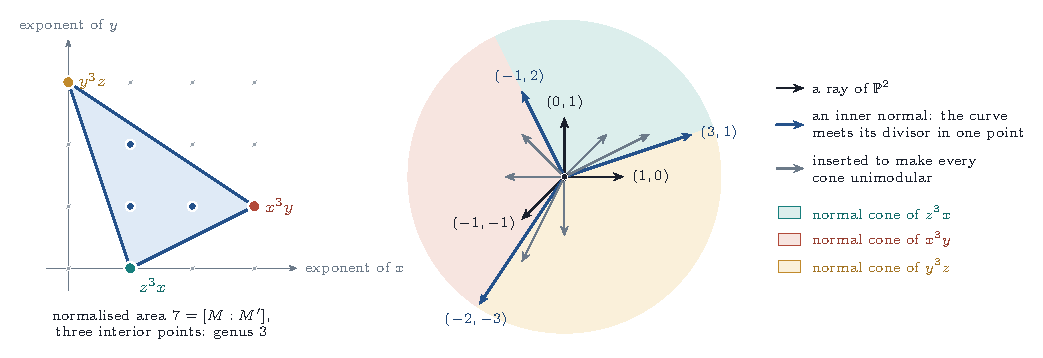
\includegraphics[width=\textwidth]{fig_simplextype}
\caption{The Klein quartic $x^{3}y+y^{3}z+z^{3}x$ in the proof of
\Cref{thm:simplextype}. Left: its Newton triangle in the lattice $M$ of the
torus of $\PP^{2}$, in the chart $z=1$, with normalised area $7=[M:M']$ and
three interior points, the genus. Right: the rays of a smooth fan adapted to
it, the three rays of $\PP^{2}$, the three inner normals of the triangle and
the six rays inserted to make every cone unimodular. The curve meets only
the three divisors of the inner normals, in one point each, the lattice
length of the edge, so its Euler number is $-7+3=-4$. With $e_{A}=7$ the
isogeny of the proof makes it the quotient of the Fermat septic by a group
of order seven.}
\label{fig:simplextype}
\end{figure}

The Fermat hypersurfaces are the complete intersections of one diagonal
hypersurface. Complete intersections of several diagonal hypersurfaces of
the same degree lie in $\mathcal{A}$ as well when their coefficients are of
Vandermonde type, because they are quotients of powers of one curve. Fix
$d\ge2$, $N\ge2$ and $1\le c\le N-1$, put $r=N-c$, and call a $c\times(N+1)$
matrix $(a_{ki})$ \emph{of Vandermonde type} if there are distinct
$\lambda_{0},\dots,\lambda_{N}\in\CC$, nonzero $\mu_{0},\dots,\mu_{N}$ and
$g\in\mathrm{GL}_{c}(\CC)$ with
$a_{ki}=\mu_{i}\sum_{l=1}^{c}g_{kl}\lambda_{i}^{l-1}$; for $c\ge2$ this says
that the columns are distinct points of a rational normal curve of degree
$c-1$ in $\PP^{c-1}$. Put $w_{i}=\prod_{l\ne i}(\lambda_{i}-\lambda_{l})^{-1}$
and
\[
  X_{d,r}(\lambda)=\Bigl\{x\in\PP^{N}:\ \sum_{i=0}^{N}w_{i}\lambda_{i}^{k}x_{i}^{d}=0,
  \ \ 0\le k\le c-1\Bigr\}.
\]
For $r=1$ this is the generalised Fermat curve of type $(d,N)$ of
Gonz\'alez-Diez, Hidalgo and Leyton \cite{GDHL09}, the Galois cover of
$\PP^{1}$ with group $H=\mu_{d}^{N+1}/\mu_{d}$, acting by
$u_{i}\mapsto h_{i}u_{i}$, branched over the $\lambda_{i}$. The characters of
$H$ are the $\chi_{a}(h)=\prod_{i}h_{i}^{a_{i}}$ with
$a\in(\ZZ/d)^{N+1}$ and $\sum_{i}a_{i}=0$; write $V_{a}\subset
H^{1}(C,\CC)$ for the eigenspace on which $h^{*}$ acts by $\chi_{a}(h)$, $[a]$
for the orbit of $a$ under $(\ZZ/d)^{\times}$, and $B_{[a]}$ for the image of
a multiple of the idempotent of $\QQ[H]$ attached to $[a]$, an abelian
subvariety of the Jacobian $J(C)$ whose first cohomology is the part
$\bigoplus_{a'\in[a]}V_{a'}$ of $H^{1}(C,\CC)$.

\begin{theorem}[Diagonal complete intersections of Vandermonde
type]\label{thm:vandermonde}
Let $X\subset\PP^{N}$ be the complete intersection of $c$ hypersurfaces
$\sum_{i}a_{ki}x_{i}^{d}=0$, $1\le k\le c$, with $(a_{ki})$ of Vandermonde
type, and let $C=X_{d,1}(\lambda)$ for the $\lambda_{i}$ of $(a_{ki})$.
\begin{enumerate}[label=\textup{(\roman*)},leftmargin=2.6em,itemsep=2pt]
\item $X$ is smooth of dimension $r$ and isomorphic to $X_{d,r}(\lambda)$,
  and $C$ is a smooth curve of genus
  $1+\tfrac12d^{N-1}\bigl((N-1)(d-1)-2\bigr)$.
\item The map
  $\Phi(u^{(1)},\dots,u^{(r)})=\bigl(\prod_{j}u^{(j)}_{i}\bigr)_{i}$ is a
  surjective morphism $C^{r}\to X_{d,r}(\lambda)$, and it induces an
  isomorphism $C^{r}/G\cong X_{d,r}(\lambda)$, where $G$ is the group of
  order $r!\,d^{N(r-1)}$ generated by the permutations of the factors and the
  $(h_{1},\dots,h_{r})\in H^{r}$ with $h_{1}\cdots h_{r}=1$.
\item $X\in\mathcal{A}$, so \textup{(F3$'$)} holds on $X$ in every degree.
\item $\dim V_{a}=\#\{i:a_{i}\ne0\}-2$ for $a\ne0$, and the Hodge conjecture
  holds on $X$ as soon as it holds on the abelian varieties $B_{[a]}$ with
  $\dim V_{a}\ge r$, which have dimension $\tfrac12|[a]|\dim V_{a}$.
\end{enumerate}
\end{theorem}

\begin{proof}
Everything rests on the Lagrange identity: interpolating a polynomial $f$
of degree at most $N$ at the $\lambda_{i}$ and comparing the coefficients of
$t^{N}$ gives $\sum_{i}w_{i}f(\lambda_{i})=0$ when $\deg f\le N-1$.%
\footnote{Lagrange interpolation writes
$f(t)=\sum_{i}f(\lambda_{i})\prod_{l\ne i}(t-\lambda_{l})/(\lambda_{i}-\lambda_{l})$
for $\deg f\le N$, and the coefficient of $t^{N}$ on the right is
$\sum_{i}w_{i}f(\lambda_{i})$. For $N=2$ and $f=1$ it says that
$\sum_{i}\prod_{l\ne i}(\lambda_{i}-\lambda_{l})^{-1}=0$ for any three
distinct numbers. The
identity says that the vector $(w_{i}\lambda_{i}^{k})_{i}$ is orthogonal to the
values of every polynomial of degree at most $N-1-k$, which is how the
equations of $X_{d,r}(\lambda)$ become the condition that the $d$-th powers of
the coordinates are the values of one polynomial of degree at most $r$.}

(i) Replacing the equations by their combinations under $g^{-1}$ and $x_{i}$
by $\nu_{i}x_{i}$ with $\nu_{i}^{d}\mu_{i}=w_{i}$ turns them into those of
$X_{d,r}(\lambda)$. Every $c\times c$ minor of $(a_{ki})$ is
$\det g\prod\mu_{i}$ times a Vandermonde determinant in distinct
$\lambda_{i}$, so any $c$ columns are independent. At a point $x$ of $X$ the
Jacobian matrix is $(d\,a_{ki}x_{i}^{d-1})$; if $S=\{i:x_{i}\ne0\}$ had at most
$c$ elements, $\sum_{i\in S}x_{i}^{d}a_{i}=0$ would be a relation between at
most $c$ columns, so $|S|>c$ and the Jacobian has rank $c$.%
\footnote{The columns of the Jacobian matrix with $i\in S$ are the columns of
$(a_{ki})$ multiplied by the nonzero numbers $d\,x_{i}^{d-1}$, and any $c$ of
the columns of $(a_{ki})$ are independent; so $c$ of them already give rank
$c$. Without the Vandermonde condition this fails: for two diagonal
quadrics in $\PP^{3}$ with proportional columns $i=0,1$, the points with
$x_{2}=x_{3}=0$ and $a_{0}x_{0}^{2}+a_{1}x_{1}^{2}=0$ are singular.} Hence $X$ is a
smooth complete intersection of dimension $r$, connected because $r\ge1$, and
the same holds for $C$. The genus follows from the Riemann--Hurwitz formula
for the cover $C\to\PP^{1}$ of degree $d^{N}$ described below, which has
$N+1$ branch points of ramification index $d$.

(ii) For $1\le k\le N-1$ let $\Lambda_{k}$ be the space of
$y\in\CC^{N+1}$ with $\sum_{i}w_{i}\lambda_{i}^{l}y_{i}=0$ for
$0\le l\le N-k-1$. The vectors $(F(\lambda_{i}))_{i}$ with $\deg F\le k$ lie
in $\Lambda_{k}$ by the identity, since $\deg t^{l}F\le N-1$; they form a space
of dimension $k+1$, since $k<N+1$; and $\Lambda_{k}$ has dimension $k+1$,
the $N-k$ equations having independent Vandermonde rows. So
$\Lambda_{k}=\{(F(\lambda_{i}))_{i}:\deg F\le k\}$, and $C$ and
$X_{d,r}(\lambda)$ are the sets of points whose $d$-th powers lie in
$\Lambda_{1}$ and in $\Lambda_{r}$. The point $u\in C$ determines
$(s:t)\in\PP^{1}$ with $u_{i}^{d}=\kappa(t-\lambda_{i}s)$ for all $i$; this is
the quotient $C\to C/H=\PP^{1}$, whose fibres are the $H$-orbits. If
$(u^{(j)}_{i})^{d}=t_{j}-\lambda_{i}s_{j}$, then
$\Phi(u)_{i}^{d}=F(\lambda_{i})$ for $F(t)=\prod_{j}(t_{j}-ts_{j})$, a nonzero
polynomial of degree at most $r<N+1$; so $\Phi(u)\in X_{d,r}(\lambda)$ and
$\Phi(u)\ne0$, and $\Phi$, given by forms of multidegree $(1,\dots,1)$ with no
common zero, is a morphism. It is $G$-invariant. Conversely, if $x\in
X_{d,r}(\lambda)$, then $(x_{i}^{d})_{i}=(F(\lambda_{i}))_{i}$ for a unique
nonzero $F$ of degree at most $r$, which factors as
$\prod_{j}(t_{j}-ts_{j})$, uniquely up to order and to rescaling the factors.
Choosing $u^{(j)}$ over $(s_{j}:t_{j})$ gives $\Phi(u)_{i}=\epsilon_{i}x_{i}$
with $\epsilon_{i}\in\mu_{d}$, and multiplying $u^{(1)}$ by
$(\epsilon_{i}^{-1})$ gives a preimage.\enlargethispage{2pt} Two preimages have the same roots, so
after a permutation $u'^{(j)}=h_{j}u^{(j)}$ with $h_{j}\in H$, and $\prod_{j}h_{j}$
acts trivially on the coordinates where $x_{i}\ne0$; where $x_{i}=0$ some
$u^{(j)}_{i}$ vanishes and $h_{j,i}$ may be changed freely, so we may take
$\prod_{j}h_{j}=1$. Hence the fibres of $\Phi$ are the $G$-orbits, $\Phi$
induces a finite bijective morphism from the normal variety $C^{r}/G$ to the
smooth variety $X_{d,r}(\lambda)$, and by Zariski's main theorem this is an
isomorphism.%
\footnote{In characteristic zero a finite morphism that is bijective on
closed points is generically \'etale of degree one, hence birational, and a
finite birational morphism onto a normal variety is an isomorphism
\cite[Chapter~III, Corollary~11.4]{Har77}. The group $G$ acts faithfully on $C^{r}$,
since $H$ is the group of deck transformations of $C\to\PP^{1}$, so
$\Phi$ has degree $|G|$.}
The order of $G$ is $r!\,|H|^{r-1}$.

(iii) $C$ is a curve, so $C^{r}\in\mathcal{A}$, and $X$ is the image of
$C^{r}$ under a surjective morphism (\Cref{prop:f3prime}(iii)).

(iv) For $a\ne0$, the forms
$t^{j}\prod_{i}(t-\lambda_{i})^{-b_{i}/d}\,dt$ with $b_{i}\in\{0,\dots,d-1\}$,
$b_{i}\equiv-a_{i}$, and $0\le j\le\sum_{i}b_{i}/d-2$, are holomorphic on $C$
and span the $\chi_{a}$-eigenspace of $H^{1,0}(C)$;%
\footnote{On the affine chart $s=1$ put $u_{i}^{d}=t-\lambda_{i}$, so that the
form is $t^{j}\prod_{i}u_{i}^{-b_{i}}\,dt$ and $h\in H$ multiplies it by
$\prod_{i}h_{i}^{-b_{i}}=\chi_{a}(h)$; it is well defined on
$H=\mu_{d}^{N+1}/\mu_{d}$ because $\sum_{i}b_{i}\equiv0$. Over $\lambda_{i}$
the cover is ramified of index $d$, with a local parameter $z$ satisfying
$z^{d}=t-\lambda_{i}$, and the form is a unit times
$z^{-b_{i}}\,d(z^{d})=d\,z^{d-1-b_{i}}\,dz$, holomorphic as $b_{i}\le d-1$.
Over $t=\infty$, with $w=1/t$ and $v^{d}=w$, it is a unit times
$v^{\,d(\sum_{i}b_{i}/d-j-2)+d-1}\,dv$, holomorphic exactly when
$j\le\sum_{i}b_{i}/d-2$, the exponent of $v$ being an integer. Forms with
different characters, or with different $j$, are independent, and their
number is
$\tfrac12\sum_{a\ne0}\bigl(\#\{i:a_{i}\ne0\}-2\bigr)
=\tfrac12\bigl((N+1)(d^{N}-d^{N-1})-2(d^{N}-1)\bigr)$, which is the genus of
(i); so they form a basis of $H^{1,0}(C)$, and each eigenspace is spanned by
the forms of its character. For $d=2$ and $N=4$ they are the five forms
$dt/\sqrt{(t-\lambda_{i_{1}})\cdots(t-\lambda_{i_{4}})}$, one for each choice
of four of the five indices, on a curve of genus five.}
its dimension
$\sum_{i}\langle-a_{i}/d\rangle-1$ and that of the $\chi_{-a}$-eigenspace add up
to $\#\{i:a_{i}\ne0\}-2$, and $H^{1}(C)^{H}=H^{1}(\PP^{1})=0$. The group $H$
acts trivially on $H^{0}(C)$ and $H^{2}(C)$, so a tensor in
$H^{r}(C^{r})=\bigoplus\bigotimes_{j}H^{k_{j}}(C)$ invariant under the
$(h_{j})$ with $\prod_{j}h_{j}=1$ has all its factors in $H^{1}$, with one
character, or none: taking $h$ in one factor and $h^{-1}$ in another shows
that two factors carry the same character, and a factor in $H^{0}$ or
$H^{2}$ carries the trivial one. Taking the invariants of the permutations,
\[
  H^{r}(C^{r},\CC)^{G}=\CC\,\eta\;\oplus\;\bigoplus_{a\ne0}\textstyle\bigwedge^{r}V_{a},
\]
with $\eta$ the symmetrised product of $r/2$ classes of points when $r$ is
even and $\eta=0$ otherwise, and $W_{[a]}=\bigoplus_{a'\in[a]}\bigwedge^{r}V_{a'}$
is a sub-Hodge structure defined over $\QQ$, zero unless $\dim V_{a}\ge r$.
Let $\psi\colon C\to B_{[a]}$ be an Abel--Jacobi map followed by the
projection, so that $\psi^{*}$ maps $H^{1}(B_{[a]},\QQ)$ isomorphically onto
the $[a]$-part of $H^{1}(C,\QQ)$, and let $\sigma\colon C^{r}\to B_{[a]}$ be
$\sum_{j}\psi\circ\mathrm{pr}_{j}$. Then
$\sigma^{*}(\alpha_{1}\wedge\dots\wedge\alpha_{r})=\prod_{k}\sum_{j}
\mathrm{pr}_{j}^{*}\psi^{*}\alpha_{k}$, whose component in
$H^{1}(C)^{\otimes r}$ is the alternating sum of the
$\psi^{*}\alpha_{1}\otimes\dots\otimes\psi^{*}\alpha_{r}$. The K\"unneth
projectors of a curve are algebraic,%
\footnote{For a curve $C$ with a point $o$ they are $\pi_{0}=[o\times C]$,
$\pi_{2}=[C\times o]$ and $\pi_{1}=[\Delta_{C}]-\pi_{0}-\pi_{2}$, and
$\pi_{1}^{\otimes r}$ is their exterior product on $C^{r}\times C^{r}$. The
average $e_{G}=|G|^{-1}\sum_{g\in G}[\Gamma_{g}]$ of the graphs of the
elements of $G$ acts on $H^{*}(C^{r})$ as the projector onto the invariants,
and $\Phi^{*}$ identifies $H^{*}(X_{d,r}(\lambda),\QQ)$ with
$H^{*}(C^{r},\QQ)^{G}$.} and so is the average $e_{G}$ over $G$,
so $e_{G}\circ\pi_{1}^{\otimes r}\circ\sigma^{*}$ is induced by an algebraic
cycle on $B_{[a]}\times C^{r}$, and it maps $H^{r}(B_{[a]},\QQ)$ onto
$W_{[a]}$: the alternating tensors in the $[a]$-part are the image of
$\pi_{1}^{\otimes r}\circ\sigma^{*}$, and $e_{G}$ keeps those of one
character. A surjective morphism of polarisable Hodge structures maps Hodge
classes onto Hodge classes,%
\footnote{The category of polarisable rational Hodge structures is semisimple,
so the kernel of a surjective morphism $f\colon V\to W$ has a complement
$V'$, a sub-Hodge structure that $f$ maps isomorphically onto $W$; a Hodge
class of $W$ is then the image of a Hodge class of $V'$.} so the Hodge classes of $W_{[a]}$ are algebraic
when those of $B_{[a]}$ are. Now let $x$ be a Hodge class of degree $r$ on
$X=X_{d,r}(\lambda)$, the other degrees being multiples of powers of the
hyperplane class by the Lefschetz hyperplane theorem. Then $\Phi^{*}x$ is a
$G$-invariant Hodge class, its components in the $W_{[a]}$ and along $\eta$
are Hodge classes, being cut out by the algebraic projectors attached to
the action of $H^{r}$, and they are algebraic; so $\Phi^{*}x$ is algebraic,
and so is $x=\Phi_{*}\Phi^{*}x/|G|$.\enlargethispage{2pt} Finally $\dim B_{[a]}$ is half of
$\sum_{a'\in[a]}\dim V_{a'}=|[a]|\dim V_{a}$.
\end{proof}

\begin{corollary}[Two diagonal hypersurfaces]\label{cor:twodiagonal}
\leavevmode
\begin{enumerate}[label=\textup{(\roman*)},leftmargin=2.6em,itemsep=2pt]
\item Every smooth complete intersection of two diagonal hypersurfaces
  $\sum_{i}a_{i}x_{i}^{d}=\sum_{i}b_{i}x_{i}^{d}=0$ of the same degree in
  $\PP^{N}$ is of Vandermonde type, so it lies in $\mathcal{A}$ and
  satisfies \textup{(F3$'$)} in every degree.
\item Let $d\in\{3,4,6\}$ and $N\le6$, or $d=2$ and $N\le12$. Then the
  Hodge conjecture holds on every complete intersection of Vandermonde type
  in $\PP^{N}$ of $N-r$ diagonal hypersurfaces of degree $d$. In particular
  it holds on every smooth complete intersection of two diagonal
  hypersurfaces of degree $3$, $4$ or $6$ in $\PP^{6}$.
\item For $d\in\{3,4,6\}$ and $N=6$, each orbit $[a]$ of order at least
  three with six nonzero coordinates and $\sum_{i}\langle a_{i}/d\rangle=3$ makes $B_{[a]}$ an
  abelian fourfold of Weil type for $K=\QQ(\zeta_{d})$, and $W_{[a]}$ is its
  space of Weil classes. On each of these fourfolds $X$ the Weil classes of
  the $70$, $490$ and $6125$ such orbits, for $d=3,4,6$, give Hodge classes of
  degree four outside $\QQ h^{2}$, so the Hodge classes of $X$ form a space of
  dimension at least $141$, $981$ and $12251$, whereas the divisor classes of
  $X$ are the multiples of $h$.
\end{enumerate}
\end{corollary}

\begin{proof}
(i) If two columns $(a_{i},b_{i})$ and $(a_{j},b_{j})$ were proportional,
or one of them zero, $X$ would contain a point supported on $\{i,j\}$, or
the coordinate point $e_{i}$, at which the Jacobian has rank at most one;
so the $N+1$ columns are distinct points of $\PP^{1}$. Sending a point of
$\PP^{1}$ outside them to infinity writes them as
$\mu_{i}(1,\lambda_{i})$ with distinct $\lambda_{i}$, which is the
Vandermonde form for $c=2$, and \Cref{thm:vandermonde}(iii) applies.
(ii) For $d\in\{2,3,4,6\}$ every $a$ has order $1$, $2$, $3$, $4$ or $6$, so
$|[a]|\le2$, with $|[a]|=1$ for the $a$ of order two, whose $V_{a}$ is real,
so that $\dim B_{[a]}\le\dim V_{a}\le N-1$. When $d=2$ every $a\ne0$ has
order two and an even number of nonzero coordinates, at most $12$ when
$N\le12$, so $\dim B_{[a]}=\tfrac12\dim V_{a}\le5$. So every $B_{[a]}$ has
dimension at most five,%
\footnote{Both bounds are sharp: for $d=3$ and $N=7$ a character with eight
nonzero coordinates has $\dim V_{a}=6$ and $|[a]|=2$, so $\dim B_{[a]}=6$;
for $d=2$ and $N=13$ a character with fourteen nonzero coordinates has
$\dim B_{[a]}=6$.} and the Hodge
conjecture holds on abelian varieties of dimension at most five
\cite{Mar25a,Mar25b,MZ99}; \Cref{thm:vandermonde}(iv) gives the conclusion,
and (i) the last statement.
(iii) For such $a$ the eigenspaces $V_{a}$ and $V_{-a}$ have dimension four
and contain two-dimensional parts of type $(1,0)$, so $K$ acts on
$H^{1,0}(B_{[a]})$ with multiplicities $(2,2)$ and $B_{[a]}$, of dimension
four, is of Weil type; $\bigwedge^{4}V_{a}$ and $\bigwedge^{4}V_{-a}$ are its
Weil lines, of type $(2,2)$ for every $\lambda$, and they lie in
$H^{4}(C^{4})^{G}=\Phi^{*}H^{4}(X)$. The zero coordinate of $a$ is one of
seven, and the other six $a_{i}\in\{1,\dots,d-1\}$ add up to $3d$, which
they do in $20$, $141$ and $1751$ ways for $d=3,4,6$, the coefficients of
$x^{3d-6}$ in $(1+x+\dots+x^{d-2})^{6}$; removing the character of order two
with every $a_{i}=d/2$ leaves $20$, $140$ and $1750$, and $(\ZZ/d)^{\times}=
\{\pm1\}$ pairs them off, since $-a$ again has coordinate sum $3d$; this
gives $7\cdot20/2=70$, $7\cdot140/2=490$ and $7\cdot1750/2=6125$ orbits.
Distinct orbits give independent classes, and the hyperplane class
lies in the part of the trivial character, which gives the bounds; the
Picard group of a complete intersection of dimension at least three is
generated by $h$.
\end{proof}

\Cref{fig:vandermonde} draws the construction. For $c=1$ the theorem is \Cref{prop:aclosure}(iii) again,
by a different route, and for $r=1$ it restates the definition of $C$.

\begin{figure}[tbp]
\centering
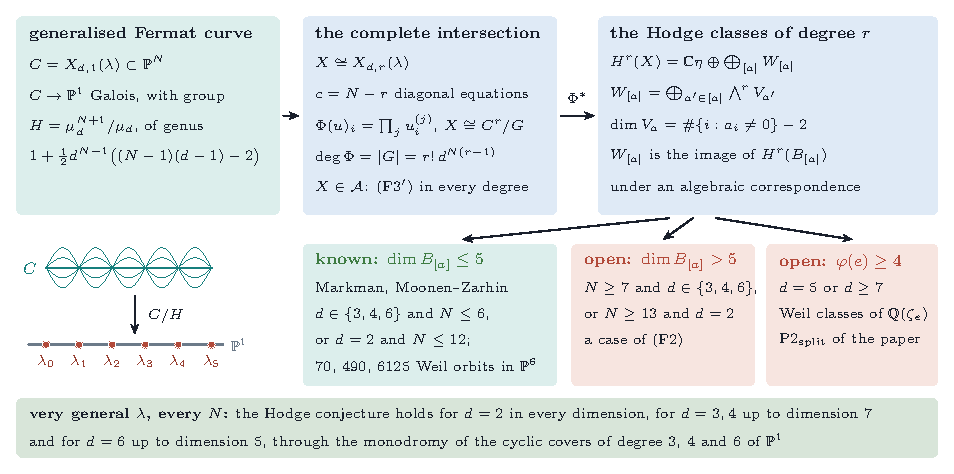
\includegraphics[width=\textwidth]{fig_vandermonde}
\caption{\Cref{thm:vandermonde} and \Cref{cor:twodiagonal}. Left: the
generalised Fermat curve $C$ over $\PP^{1}$, its sheets meeting over the
branch points $\lambda_{0},\dots,\lambda_{N}$ (five sheets stand for the
$d^{N}$ of the cover). Top: $C$, the complete intersection
$X\cong C^{r}/G$ with the map $\Phi$ of degree $|G|$, and the decomposition
of $H^{r}(X)$ through $\Phi^{*}$. Bottom: where the Hodge conjecture for $X$
stands at an arbitrary configuration, according to the abelian varieties
$B_{[a]}$ that carry its Hodge classes: known when they have dimension at
most five, which happens for $d\in\{3,4,6\}$ and $N\le6$ and for $d=2$ and
$N\le12$, and open when they are larger, a case of (F2), or carry Weil
classes of $\QQ(\zeta_{e})$ with $\varphi(e)\ge4$, the case
$\mathrm{P2}_{\mathrm{split}}$ of the paper. Foot: the very general
configuration, \Cref{thm:vgvandermonde}.}
\label{fig:vandermonde}
\end{figure}

At a very general configuration the abelian varieties $B_{[a]}$ carry only
the Hodge classes that the monodromy of the curves allows, and the
conjecture can then be decided in every dimension for $d=2$, up to dimension
seven for $d=3$ and $d=4$, and up to dimension five for $d=6$. Write $U\subset\CC^{N+1}$ for the space of
$(N+1)$-tuples of distinct numbers. The varieties $X_{d,r}(\lambda)$ with
$\lambda\in U$ form a smooth projective family over $U$, and so do the
curves $C$ and the maps $\Phi$, with $H$ acting on the family of curves.

\begin{lemma}[Hodge classes of a very general member]\label{lem:vgmonodromy}
Let $\mathbb{V}$ be a polarised variation of $\ZZ$-Hodge structure of weight
$2p$ on a smooth connected quasi-projective variety $S$, and let
$\Pi=\pi_{1}(S,s)$ act on $\mathbb{V}_{s}$. If $s$ lies outside a countable
union of proper Zariski closed subsets of $S$, the space $\Hdg(\mathbb{V}_{s})$
of rational classes of type $(p,p)$ is stable under $\Pi$, and a subgroup of
finite index of $\Pi$ fixes it pointwise.
\end{lemma}

\begin{proof}
The locus of Hodge classes has countably many components
(\cite[Definition~B.3]{paperI}, \cite[Lemma~B.4]{paperI}), and the image in $S$ of
each is Zariski closed (\cite[Theorem~B.6]{paperI}); let $s$ avoid the images that are
not all of $S$. For $\alpha\in\Hdg(\mathbb{V}_{s})$ the component through
$(s,\alpha)$ maps onto $S$, locally biholomorphically onto its image, so the
flat section $\tilde\alpha$ through $\alpha$ on the universal cover $\tilde S$
is of type $(p,p)$ on a nonempty open set. The set where it is of type
$(p,p)$ is a closed analytic subset of the connected manifold $\tilde S$, so it
is all of $\tilde S$, and every transport of $\alpha$ along a loop at $s$ is a
Hodge class at $s$. The group $\Pi$ therefore preserves
$\Hdg(\mathbb{V}_{s})$, the lattice $\mathbb{V}_{s,\ZZ}\cap\Hdg(\mathbb{V}_{s})$
and the flat form $\tilde Q$ of the proof of \cite[Lemma~B.5]{paperI}, which is
positive definite on the real classes of type $(p,p)$; so it acts on
$\Hdg(\mathbb{V}_{s})$ through a finite group, whose kernel is the subgroup
of the statement.
\end{proof}

For the characters of order three, four and six the monodromy of the
curves $D_{a}$ is determined by induction on the number of branch points. The
step lets two branch points collide, and a lemma on two copies of $\SL$ of a
hyperplane closes it. The base has four branch points, two of them with
opposite exponents, whose full twist is a transvection
(\Cref{fig:cyclicmerge}).

\begin{setupenv}[Cyclic covers]\label{setup:cyclic}
Let $m\in\{3,4,6\}$, $\zeta=e^{2\pi i/m}$ and $K=\QQ(\zeta)$, and let
$a=(a_{1},\dots,a_{k})$ with $a_{i}\in\ZZ/m$ nonzero, $\sum_{i}a_{i}=0$ and
$\gcd(m,a_{1},\dots,a_{k})=1$, so that $a$ has order $m$. For $\lambda$ in
the space $\mathrm{Conf}_{k}$ of $k$-tuples of distinct complex numbers let
$D_{a}$ be the cyclic cover $y^{m}=\prod_{i}(t-\lambda_{i})^{a_{i}}$ of
$\PP^{1}$, with representatives $0<a_{i}<m$; it is unramified over
$\infty$. Let $V_{a}\subset H^{1}(D_{a},\CC)$ be the eigenspace of the deck
group on which $H^{1,0}$ is spanned by the forms
$t^{j}\prod_{i}(t-\lambda_{i})^{-b_{i}/m}\,dt$, where $0<b_{i}<m$, $b_{i}\equiv
-a_{i}$ and $0\le j\le\sum_{i}b_{i}/m-2$ \cite[\S2]{DM86}, and put
$n=\dim V_{a}$,
$p=\dim V_{a}^{1,0}=\sum_{i}b_{i}/m-1$ and $q=n-p$. Let $\Gamma_{a}\subset
\GL(V_{a})$ be the image of the pure braid group
$P_{k}=\pi_{1}(\mathrm{Conf}_{k})$ and $G_{a}^{0}$ the identity component of
its Zariski closure.
\end{setupenv}

\begin{lemma}[A model of the monodromy]\label{lem:foxmodel}
Let $F_{k}$ be the free group on loops $x_{1},\dots,x_{k}$ around
$\lambda_{1},\dots,\lambda_{k}$, put $t_{i}=\zeta^{a_{i}}$, let
$\partial\colon K^{k}\to K$ map $e_{i}$ to $t_{i}-1$, and let
$E_{a}=\ker\partial/K\ell$, where $\ell=\sum_{i}t_{1}\cdots t_{i-1}e_{i}$. A pure
braid $\beta$ acts on $F_{k}$ by Artin's automorphism and on $K^{k}$ by
$v\mapsto vJ_{\beta}$, where $J_{\beta}$ is the matrix of Fox derivatives
$\partial\beta(x_{i})/\partial x_{j}$ evaluated at $x_{j}\mapsto t_{j}$. This
action preserves $\ker\partial$ and fixes $\ell$, and the representation of
$P_{k}$ on $E_{a}$, of dimension $k-2$, is isomorphic to $V_{a}$, to its dual
or to its complex conjugate. So $n=k-2$, and $G_{a}^{0}\supseteq\SL(V_{a})$ if
and only if the identity component of the Zariski closure of the image of
$P_{k}$ in $\GL(E_{a})$ contains $\SL(E_{a})$.
\end{lemma}

\begin{proof}
Fox's formula $\sum_{j}(\partial w/\partial x_{j})(x_{j}-1)=w-1$ \cite{Fox53},
evaluated at $x_{j}\mapsto t_{j}$, shows that the vector
$\sum_{j}(\partial w/\partial x_{j})(t)\,e_{j}$ of a word $w$ with $t(w)=1$ lies
in $\ker\partial$. It is the class of the lift of the loop $w$ in the summand
of $H_{1}(D_{a}^{\circ},K)$ on which the deck group acts through
$x_{i}\mapsto t_{i}$, where $D_{a}^{\circ}$ is the unramified part of the
cover, and that summand is $H_{1}(F_{k},K_{t})=\ker\partial$, computed from the
free resolution of length one of the augmentation ideal of a free group.%
\footnote{By Shapiro's lemma $H_{1}(D_{a}^{\circ},K)=H_{1}(F_{k},K[\mu_{m}])$,
and its summand for the character $x_{i}\mapsto t_{i}$ is $H_{1}(F_{k},K_{t})$.
The augmentation ideal of $\ZZ[F_{k}]$ is free on the $x_{i}-1$, so
$H_{1}(F_{k},K_{t})$ is the kernel of $\bigoplus_{i}Ke_{i}\to K$,
$e_{i}\mapsto t_{i}-1$, the chain $e_{i}$ standing for the loop $x_{i}$ and a word
$w$ for $\sum_{j}(\partial w/\partial x_{j})(t)e_{j}$.} Filling in the points
over $\lambda_{i}$ adds no relation: the loop around such a point lifts
$x_{i}^{e}$, $e$ the order of $t_{i}$, whose vector
$(1+t_{i}+\dots+t_{i}^{e-1})e_{i}$ is zero. Filling in the $m$ points over
$\infty$, where the cover is unramified, kills the lift of $x_{1}\cdots
x_{k}$, whose vector is $\ell\ne0$. So $E_{a}$ is the summand of
$H_{1}(D_{a},K)$ for the character $x_{i}\mapsto t_{i}$, of dimension $k-2$. A
pure braid fixes $x_{1}\cdots x_{k}$ and maps each $x_{i}$ to a conjugate of
itself, so it preserves $t$, and the chain rule for Fox derivatives makes
$\beta\mapsto J_{\beta}$ the action of $P_{k}$ on this summand.%
\footnote{Artin's automorphism of the half twist $\sigma_{i}$ of the $i$-th
and $(i+1)$-st points is $x_{i}\mapsto x_{i}x_{i+1}x_{i}^{-1}$,
$x_{i+1}\mapsto x_{i}$, the other generators being fixed; $P_{k}$ is generated
by the full twists $A_{st}=\sigma_{t-1}\cdots\sigma_{s+1}\sigma_{s}^{2}
\sigma_{s+1}^{-1}\cdots\sigma_{t-1}^{-1}$. For a pure braid the chain rule
reads $J_{\beta\beta'}=J_{\beta'}J_{\beta}$ or $J_{\beta}J_{\beta'}$, according
to the convention for composing braids, with no twist of the coefficients,
since $t\circ\beta=t$.} Poincar\'e duality and the choice of the generator
of the deck group identify it with $V_{a}$, its dual or its conjugate, and
the automorphisms $g\mapsto{}^{t}g^{-1}$ and $g\mapsto\bar g$ of $\GL$ preserve
$\SL$.
\end{proof}

\begin{lemma}[Collision of two branch points]\label{lem:cabling}
In \Cref{lem:foxmodel} suppose that $a_{1}+a_{2}\ne0$, and let
$a'=(a_{1}+a_{2},a_{3},\dots,a_{k})$. Let $I=(1-t_{2})e_{1}-(1-t_{1})e_{2}$,
the cycle of a disc around $\lambda_{1}$ and $\lambda_{2}$, and let
$Y\subset E_{a}$ be the image of the cycles outside that disc, the vectors of
$\ker\partial$ with $v_{2}=t_{1}v_{1}$. Then $E_{a}=Y\oplus KI$, and
$\iota(v_{1},v_{3},\dots,v_{k})=(v_{1},t_{1}v_{1},v_{3},\dots,v_{k})$ induces an
isomorphism $E_{a'}\to Y$. If $\beta\in P_{k}$ is obtained from
$\beta'\in P_{k-1}$ by doubling its first strand, then $\beta$ preserves $Y$
and $KI$, acts on $Y$ as $\beta'$ acts on $E_{a'}$, and multiplies $I$ by a
power of $\zeta$.
\end{lemma}

\begin{proof}
The vectors of $Y$ have $(v_{1},v_{2})$ proportional to $(1,t_{1})$, and
$(1-t_{2},t_{1}-1)$ is proportional to $(1,t_{1})$ only if $t_{1}t_{2}=1$; so
$I\notin Y$. The map $\iota$ carries the kernel of $\partial'$, where
$\partial'(e_{1})=t_{1}t_{2}-1$, onto the cycles outside the disc, because
$v_{1}(t_{1}t_{2}-1)=v_{1}(t_{1}-1)+t_{1}v_{1}(t_{2}-1)$, and it carries the
vector $\ell'$ of $a'$ to $\ell$; as $\dim E_{a'}+1=\dim E_{a}$, both
assertions about $Y$ follow. The doubled braid moves a disc containing
$\lambda_{1},\lambda_{2}$ rigidly. Its automorphism therefore maps
$x_{1}\mapsto wx_{1}w^{-1}$, $x_{2}\mapsto wx_{2}w^{-1}$ and $x_{j}\mapsto
u_{j}$ for $j\ge3$, where $y\mapsto w'yw'^{-1}$, $x_{j}\mapsto u_{j}'$ is the
automorphism of $\beta'$ on the free group on $y,x_{3},\dots,x_{k}$, and
$w,u_{j}$ are $w',u_{j}'$ with $y$ replaced by $x_{1}x_{2}$. For such a word
$u$ the chain rule gives $\partial u/\partial x_{1}=\partial u/\partial y$
and $\partial u/\partial x_{2}=(\partial u/\partial y)\,x_{1}$, which at $t$ is
the relation $v_{2}=t_{1}v_{1}$; together with
$\partial(wx_{i}w^{-1})/\partial x_{j}=(1-t_{i})\,\partial w/\partial
x_{j}+t(w)\delta_{ij}$ at $t$, this shows that the rows of $J_{\beta}$ for
$j\ge3$, and the first row plus $t_{1}$ times the second, are the images under
$\iota$ of the rows of $J_{\beta'}$; this is the equivariance of $\iota$. The
same formula gives $IJ_{\beta}=(1-t_{2})\bigl((1-t_{1})\partial w+t(w)e_{1}\bigr)
-(1-t_{1})\bigl((1-t_{2})\partial w+t(w)e_{2}\bigr)=t(w)I$, and $t(w)$ is a
power of $\zeta$.
\end{proof}

\begin{lemma}[Two hyperplanes]\label{lem:hyperplanes}
Let $E=Y\oplus L$ be a complex vector space with $\dim Y\ge2$ and
$\dim L=1$, let $S\subset\SL(E)$ be the subgroup acting on $Y$ through
$\SL(Y)$ and trivially on $L$, and let $\gamma\in\GL(E)$ satisfy
$\gamma L\ne L$ and $\gamma Y\ne Y$. Then the group $T$ generated by $S$ and
$\gamma S\gamma^{-1}$ acts irreducibly on $E$. If $\dim Y\ge3$, then
$T=\SL(E)$. If $\dim Y=2$, every connected semisimple subgroup of $\SL(E)$
that contains $T$ is $\SL(E)$.
\end{lemma}

\begin{proof}
The group $T$ is connected. As a representation of $S$, $E$ is
the sum of the irreducible nontrivial $Y$ and the trivial $L$, so its
$S$-stable subspaces are $0$, $L$, $Y$ and $E$, and those of
$\gamma S\gamma^{-1}$ are $0$, $\gamma L$, $\gamma Y$ and $E$; by the
hypotheses and the dimensions only $0$ and $E$ are in both lists, and $T$ is
irreducible.

Let $\dim Y\ge3$. As a representation of $\mathfrak{sl}(Y)$,
\[
  \mathfrak{sl}(E)=\mathfrak{sl}(Y)\oplus\mathrm{Hom}(L,Y)\oplus
  \mathrm{Hom}(Y,L)\oplus\CC z,
\]
$z$ acting by $1$ on $Y$ and by $-\dim Y$ on $L$, and the four summands, the
adjoint representation, $Y$, $Y^{*}$ and the trivial one, are pairwise
non-isomorphic since $\dim Y\ge3$. The Lie algebra $\mathfrak{t}$ of $T$
contains $\mathfrak{sl}(Y)$ and is stable under it, so it is
$\mathfrak{sl}(Y)$ plus some of the other three summands. Without
$\mathrm{Hom}(L,Y)$ it preserves $L$, and without $\mathrm{Hom}(Y,L)$ it
preserves $Y$; both are excluded by irreducibility. The bracket of a nonzero
map $L\to Y$ with a map $Y\to L$ not vanishing on its image has a nonzero
component along $z$, so $\mathfrak{t}=\mathfrak{sl}(E)$ and $T=\SL(E)$.

Let $\dim Y=2$ and let $G\supseteq T$ be connected and semisimple. Then $E$
is a faithful irreducible representation of dimension $3$ of the Lie algebra
$\mathfrak{g}$ of $G$. An irreducible representation of a product of simple
Lie algebras is a tensor product of irreducible representations of the
factors, and $3$ is prime, so $\mathfrak{g}$ is simple. It lies in
$\mathfrak{sl}(E)$, of dimension $8$ and rank $2$, and the simple Lie
algebras of rank at most $2$ are $\mathfrak{sl}_{2}$, $\mathfrak{sl}_{3}$,
$\mathfrak{so}_{5}$ and $\mathfrak{g}_{2}$, of dimensions $3$, $8$, $10$ and
$14$. If $\mathfrak{g}\cong\mathfrak{sl}_{2}$, then $\mathfrak{g}$ equals the
Lie algebra of $S$, both being of dimension $3$, so $G=S$, which preserves
$L$, against the irreducibility of $T$. Hence $\mathfrak{g}=\mathfrak{sl}(E)$
and $G=\SL(E)$.
\end{proof}

\begin{lemma}[Merging two branch points]\label{lem:merge}
Let $m$ and $a$ be as in \Cref{setup:cyclic}, with $k\ge6$ and $p,q\ge1$.
Then there are $i\ne j$ with $a_{i}+a_{j}\ne0$ such that the vector $a'$
obtained by replacing $a_{i}$ and $a_{j}$ by $a_{i}+a_{j}$ has order $m$, and
its numbers $p'$ and $q'$ are at least $1$.
\end{lemma}

\begin{proof}
Put $f_{i}=b_{i}/m\in[1/m,1-1/m]$, so that $p+1=\sum_{i}f_{i}$ and
$q+1=\sum_{i}(1-f_{i})$. Merging $a_{i}$ and $a_{j}$ keeps $p$ and lowers $q$
by one if $f_{i}+f_{j}<1$, and lowers $p$ by one and keeps $q$ if
$f_{i}+f_{j}>1$. Since $a_{i}+a_{j}=-\sum_{l\ne i,j}a_{l}$, the order of $a'$ is
that of the subgroup generated by the $a_{l}$ with $l\ne i,j$, the rest of
$a$. Replacing $a$ by $-a$ exchanges $p$ and $q$, so we may assume $q\ge p$,
hence $q\ge2$ as $p+q=k-2\ge4$; if $p\ge2$, every merge keeps $p',q'\ge1$
and only the order matters.

\emph{The order.} For $m=3$ two equal coordinates exist, their sum is not
$0$, and any nonzero rest generates $\ZZ/3$. For $m=4$ the number of odd
coordinates is even and positive; if it is at least $4$, merge two equal odd
ones, and if it is $2$, merge an odd one with one of the at least four
coordinates equal to $2$. For $m=6$ the rest generates $\ZZ/6$ exactly when
it contains an odd coordinate and one prime to $3$. The odd coordinates
are even in number and the coordinates prime to $3$ have sum divisible by
$3$, so each kind occurs at least twice. If exactly two coordinates are
odd, the at least four others lie in $\{2,4\}$; merge two equal ones among
them. If exactly two are prime to $3$, the others equal $3$; merge a $3$
with one of the two. Otherwise each kind occurs at least three times, and
any two coordinates with nonzero sum can be merged; they exist, since
pairwise sums $0$ would force every coordinate to be $3$.

\emph{The case $p=1$.} Then $\sum_{i}b_{i}=2m$. Some $b_{i}$ equals $1$,
since otherwise $\sum_{i}b_{i}\ge2k\ge12\ge2m$, with equality only if $m=6$
and every coordinate is $4$, when $a$ has order three. Keep such a coordinate,
$a_{i}=-1$, which generates $\ZZ/m$. The other $k-1\ge5$ coordinates have
$b$-sum $2m-1$, so the two smallest values of $b$ among them add up to at most
$2(2m-1)/5<m$; merge these two coordinates. Their sum is not $0$, $p'=p=1$,
$q'=q-1=k-4\ge2$, and the rest contains $a_{i}$, so $a'$ has order $m$.
\end{proof}

\begin{lemma}[Five branch points]\label{lem:mergefive}
Let $m$ and $a$ be as in \Cref{setup:cyclic}, with $k=5$ and $p,q\ge1$. Then
$a_{i}+a_{j}=0$ for some $i\ne j$, and the other three coordinates can be
labelled $x,y,z$ so that $x+y\ne0$ and $a'=(x+y,z,a_{i},a_{j})$ has order $m$
and $p'=q'=1$.
\end{lemma}

\begin{proof}
Replacing $a$ by $-a$ we may assume $p=1$, so that $\sum_{l}b_{l}=2m$ with
five terms in $[1,m-1]$; and $a_{i}+a_{j}=0$ means $b_{i}+b_{j}=m$. For $m=3$
the terms lie in $\{1,2\}$ and exactly one is $2$; take it and a $1$. For
$m=4$, take a $3$ and a $1$ if both occur. If no term is $3$, the terms lie in
$\{1,2\}$ and at least three are $2$, which gives $2+2$; if no term is $1$,
they lie in $\{2,3\}$ and add up to at least $10$, which is impossible. For
$m=6$ suppose that no two terms add up to $6$. Then at most one term is $3$,
and neither $1$ and $5$ nor $2$ and $4$ both occur. Terms in $\{1,2,3\}$ with
at most one $3$ add up to at most $11$, and terms in $\{3,4,5\}$ to at least
$19$. Terms in $\{1,3,4\}$, respectively $\{2,3,5\}$, cannot add up to $12$,
since the number $y$ of terms $4$, respectively $5$, would satisfy
$3y\in\{7,5\}$, respectively $3y\in\{2,1\}$. This proves the first assertion.

The other three coordinates add up to $0$ and have $b$-sum $m$, so any two of
them, $x$ and $y$, have $x+y=-z\ne0$ and $b$-sum less than $m$; merging them
keeps $p'=1$, so $q'=1$, and $a'$ contains $c=a_{i}$ and $a_{j}=-c$. The order
of $a'$ is that of the subgroup generated by $z$ and $c$. If $c$ generates
$\ZZ/m$, any choice of $z$ will do. Otherwise $c$ is even, or $m=6$ and $c=3$.
As $a$ has order $m$, one of $x,y,z$ is then odd, respectively prime to $3$,
and we take it as $z$; then $z$ and $c$ generate $\ZZ/m$.
\end{proof}

\begin{proposition}[Monodromy of cyclic covers]\label{prop:cyclicmonodromy}
In \Cref{setup:cyclic}, if $p=0$ or $q=0$ then $\Gamma_{a}$ is finite, and if
$n\ge3$ and $p,q\ge1$ then $G_{a}^{0}\supseteq\SL(V_{a})$.
\end{proposition}

\begin{proof}
If $pq=0$, the polarisation is definite on $V_{a}$ up to sign, and
$\Gamma_{a}$ preserves it and the $\ZZ[\zeta]$-lattice spanned by
$H^{1}(D_{a},\ZZ)$; a discrete subgroup of a compact group is finite. Assume
$p,q\ge1$ and use the model of \Cref{lem:foxmodel}. Three facts are used
throughout. If $u\in\Gamma_{a}$ is unipotent, the Zariski closure of its
powers is the group $\exp(\tau\log u)$, so $\log u$ lies in the Lie algebra
of $G_{a}^{0}$. The group $\Gamma_{a}$ normalises $G_{a}^{0}$. And $G_{a}^{0}$
is semisimple: by Andr\'e's theorem \cite[Theorem~1]{And92} the identity
component of the Zariski closure of the monodromy group of
$H^{1}(D_{a},\QQ)$ is a normal subgroup of the derived group of the
Mumford--Tate group of a very general fibre, hence semisimple, and
$G_{a}^{0}$ is its image in $\GL(V_{a})$, the monodromy commuting with the
deck group.

\emph{Four points.} Let $k=4$, so $n=2$, and suppose that two coordinates
of $a$ are opposite; relabel them $a_{1}$ and $a_{2}$, so that $t_{1}t_{2}=1$.
The full twist $A_{12}$ maps $x_{i}\mapsto wx_{i}w^{-1}$ for $i=1,2$, with
$w=x_{1}x_{2}$, and fixes $x_{3},x_{4}$. As $t(w)=1$, the formula for
$\partial(wx_{i}w^{-1})/\partial x_{j}$ in the proof of \Cref{lem:cabling}
gives $vJ_{A_{12}}=v+\varphi(v)\,\delta$, with $\delta=e_{1}+t_{1}e_{2}$ and
$\varphi(v)=(1-t_{1})v_{1}+(1-t_{2})v_{2}$, which equals
$\sum_{j\ge3}(t_{j}-1)v_{j}$ on $\ker\partial$. Here $\delta\in\ker\partial$,
$\varphi(\delta)=0$, $\varphi(\ell)=t_{1}\cdots t_{k}-t_{1}t_{2}=0$, the
vector $\delta$ is not a multiple of $\ell$, whose third coordinate is
$t_{1}t_{2}=1$, and $\varphi\bigl((t_{3}-1)e_{1}-(t_{1}-1)e_{3}\bigr)
=-(t_{1}-1)(t_{3}-1)\ne0$. So $A_{12}$ acts on $E_{a}$ as a unipotent
$u\ne1$, and $G_{a}^{0}$ is a connected semisimple subgroup of
$\SL(E_{a})\cong\SL_{2}$ containing $\exp(\tau\log u)$. The connected
subgroups of $\SL_{2}$ of dimension one or two are solvable, so
$G_{a}^{0}=\SL(E_{a})$.

\emph{The induction.} Let $n\ge3$. If $n=3$, \Cref{lem:mergefive} gives,
after a relabelling, a vector $a'=(a_{1}+a_{2},a_{3},a_{4},a_{5})$ of order $m$
with $a_{1}+a_{2}\ne0$, $p'=q'=1$ and two opposite coordinates, so the
identity component of the Zariski closure of the monodromy of $E_{a'}$ is
$\SL(E_{a'})$ by the case of four points. If $n\ge4$, \Cref{lem:merge} and
a relabelling give $a_{1}+a_{2}\ne0$ and $a'=(a_{1}+a_{2},a_{3},\dots,a_{k})$
of order $m$ with $p',q'\ge1$, and by induction on $n$ that identity
component contains $\SL(E_{a'})$. Let $H$ be the identity component of the
Zariski closure of the doubled braids of \Cref{lem:cabling}. Then
$H\subseteq G_{a}^{0}$, $H$ preserves $Y$ and $KI$ and acts trivially on
$KI$, where the doubled braids act through a finite group, and its image in
$\GL(Y)$ is the identity component of the Zariski closure of the monodromy of
$E_{a'}$, which contains $\SL(Y)$. So $G_{a}^{0}$ contains the group $S$ of
\Cref{lem:hyperplanes} for $E_{a}=Y\oplus KI$. Let $\gamma=A_{23}$, the full
twist of the second and third points; its automorphism fixes $x_{1}$ and
maps $x_{2}\mapsto x_{2}x_{3}x_{2}x_{3}^{-1}x_{2}^{-1}$ and $x_{3}\mapsto
x_{2}x_{3}x_{2}^{-1}$. Then $\gamma(I)=I+(1-t_{1})t_{2}I_{23}$ with
$I_{23}=(1-t_{3})e_{2}-(1-t_{2})e_{3}$, and $\gamma(KI)\ne KI$, since $I$,
$I_{23}$ and $\ell$ are independent, $\ell$ having a nonzero fourth
coordinate. The functional $v\mapsto v_{2}-t_{1}v_{1}$ vanishes on $\ell$ and
cuts out $Y$, and at $\gamma(v)$ for $v\in Y$ it equals
$(t_{3}-1)(t_{1}t_{2}v_{1}-v_{3})$, which is nonzero for the cycle
$(1-t_{4})e_{3}-(1-t_{3})e_{4}$ of $Y$; so $\gamma Y\ne Y$. As $\gamma$
normalises $G_{a}^{0}$, this group contains $S$ and $\gamma S\gamma^{-1}$,
and \Cref{lem:hyperplanes}, with $\dim Y=n-1$, gives
$G_{a}^{0}=\SL(E_{a})$: for $n\ge4$ directly, and for $n=3$ because
$G_{a}^{0}$ is connected and semisimple.
\end{proof}

For $m=3$ the proposition also follows from the $\ell$-adic theorem of
Achter and Pries \cite[Corollary~3.10]{AP07}, which identifies the monodromy
of trielliptic curves with a special unitary group.

\begin{lemma}[The discriminant of the new part]\label{lem:newdisc}
In \Cref{setup:cyclic} let $n$ be even with $p=q=n/2$, let
$L=H^{1}(D_{a},\ZZ)$ with the cup product $Q$, and let
$L_{a}=L\cap(V_{a}\oplus\overline{V_{a}})$. Then $L_{a}$ is a free
$\ZZ[\zeta]$-module of rank $n$, the $K$-hermitian form $H$ with
$Q=\tfrac12\Tr_{K/\QQ}(\delta^{-1}H)$ on it, $\delta=\sqrt{-1}$ for $m=4$ and
$\delta=\sqrt{-3}$ otherwise (\cite[Lemma~4.5]{paperI}), has signature
$(n/2,n/2)$, and the class of $(-1)^{n/2}\det H$ in
$\QQ^{\times}/\Nm(K^{\times})$ is trivial for $m=3$ and $m=4$; for $m=6$ it is
trivial if and only if the number of $i$ with $a_{i}=3$ is even.
\end{lemma}

\begin{proof}
The deck transformation $g$ is an isometry of the unimodular lattice $L$, so
its eigenspaces for eigenvalues $\mu,\nu$ are orthogonal unless $\mu\nu=1$.
Hence $L_{a}$, the part for the primitive $m$-th roots of unity, and the
part $L^{\mathrm{old}}$ for the other eigenvalues are orthogonal primitive
sublattices, each the orthogonal complement of the other, and
$|\det(L_{a})|=|\det(L^{\mathrm{old}})|$, which is $1$ for $m=3$, when
$L^{\mathrm{old}}=0$.%
\footnote{If $M\subset L$ is primitive and $L$ is unimodular, restriction
$L\to M^{\vee}$ is onto with kernel $M^{\perp}$, so $L/(M\oplus M^{\perp})\cong
M^{\vee}/M$, and likewise $\cong(M^{\perp})^{\vee}/M^{\perp}$; the order of
$M^{\vee}/M$ is $|\det M|$.} For a quotient map $\pi\colon D_{a}\to D'$ of
prime degree $e$ that is ramified, $\pi^{*}H^{1}(D',\ZZ)$ is primitive in $L$
and the cup product on it is $e$ times that of $D'$.%
\footnote{A loop in $D'$ avoiding the branch points, composed with a loop
around a branch point, whose monodromy generates the group of order $e$,
lifts to a closed loop with the same image in $H_{1}(D',\ZZ)$; so
$\pi_{*}\colon H_{1}(D_{a},\ZZ)\to H_{1}(D',\ZZ)$ is onto, and its transpose
$\pi^{*}$ is a split injection. The factor $e$ is $\pi_{*}\pi^{*}=e$.} For
$m=4$, $L^{\mathrm{old}}=\pi^{*}H^{1}(D',\ZZ)$ for the quotient $D'$ by $g^{2}$,
ramified over the $\lambda_{i}$ with $a_{i}$ odd, so
$|\det L^{\mathrm{old}}|=2^{2g'}$, $g'$ the genus of $D'$. For $m=6$, the
quotients $D_{2}$ by $g^{2}$ and $D_{3}$ by $g^{3}$ are ramified over the
$\lambda_{i}$ with $3\nmid a_{i}$ and with $a_{i}$ odd, which exist since $a$
has order six, and $L^{\mathrm{old}}$ contains $A\oplus B$ with
$A=\pi_{2}^{*}H^{1}(D_{2},\ZZ)$ and $B=\pi_{3}^{*}H^{1}(D_{3},\ZZ)$, of determinants
$3^{2g_{2}}$ and $2^{2g_{3}}$; the quotient $L^{\mathrm{old}}/(A\oplus B)$ embeds in
$A^{\vee}/A$ and in $B^{\vee}/B$, of coprime orders, so $L^{\mathrm{old}}=A\oplus B$
and $|\det L^{\mathrm{old}}|=3^{2g_{2}}2^{2g_{3}}$.

On $L_{a}$ the deck transformation satisfies the cyclotomic equation of $\zeta$,
so $L_{a}$ is a torsion-free module over the principal ideal domain
$\ZZ[\zeta]$, free of rank $n$; the signature of $H$ is $(p,q)$
(\cite[Remark~4.6]{paperI}). The determinant of the trace form of a hermitian
lattice gives $|\det(L_{a})|=|d_{K}|^{n}\Nm(\tfrac{1}{2\delta})^{n}(\det H)^{2}$,
that is $(\det H)^{2}$ for $K=\QQ(i)$ and $(\det H)^{2}/4^{n}$ for
$K=\QQ(\sqrt{-3})$.%
\footnote{For a free $\cO_{K}$-module with hermitian Gram matrix $M$ and
$c\in K^{\times}$, the $\ZZ$-bilinear form $\Tr_{K/\QQ}(c\,v^{T}M\bar w)$ has
determinant of absolute value $|d_{K}|^{n}\Nm(c)^{n}(\det M)^{2}$, where
$d_{K}$ is the discriminant of $K$: for $n=1$ this is the discriminant of the
trace form of $\cO_{K}$ scaled by $\Nm(cM)$. Changing the basis by
$P\in\GL_{n}(K)$ multiplies both sides by $\Nm_{K/\QQ}(\det P)^{2}$, and a
basis in which $M$ is diagonal makes the form an orthogonal sum of forms of
rank one. Here $d_{K}=-4$ and $\Nm(\tfrac{1}{2i})=\tfrac14$, or $d_{K}=-3$ and
$\Nm(\tfrac{1}{2\sqrt{-3}})=\tfrac1{12}$.}
Hence $(-1)^{n/2}\det H$ equals $2^{n}$ for $m=3$, $2^{g'}$ for $m=4$ and
$2^{n+g_{3}}3^{g_{2}}$ for $m=6$, the sign being that of a form of signature
$(n/2,n/2)$. For $m=3$ this is $\Nm(2^{n/2})$, and for $m=4$ a norm as
$2=\Nm(1+i)$. For $m=6$, $3=\Nm(\sqrt{-3})$ and $4=\Nm(2)$
are norms and $2$ is not, since $x^{2}+xy+y^{2}$ is even only when $x$ and $y$
are, so that every norm has even $2$-adic valuation; so the class is trivial
exactly when $g_{3}$ is even. By the Riemann--Hurwitz formula $D_{3}$, the
triple cover $y^{3}=\prod_{i}(t-\lambda_{i})^{a_{i}}$ branched over the $i$
with $3\nmid a_{i}$, has genus $k-c_{3}-2=n-c_{3}$, where $c_{3}$ is the number
of $i$ with $a_{i}=3$; as $n$ is even, this is the assertion.
\end{proof}

\begin{figure}[tbp]
\centering
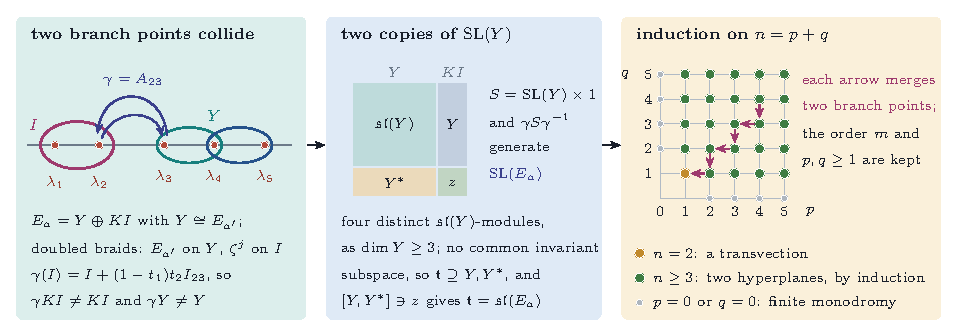
\includegraphics[width=\textwidth]{fig_cyclicmerge}
\caption{The proof of \Cref{prop:cyclicmonodromy}. Left: two branch points
$\lambda_{1},\lambda_{2}$ collide inside a disc (\Cref{lem:cabling}); the
cycles outside the disc form the hyperplane $Y\cong E_{a'}$, the cycle $I$
of the disc spans the complementary line, and the twist $\gamma$ of the
second and third points moves both. Middle: the two copies of $\SL(Y)$ of
\Cref{lem:hyperplanes}, which generate $\SL(E_{a})$ when $\dim Y\ge3$. Right: the induction on
$n=k-2$, each merge lowering $p$ or $q$ by one (\Cref{lem:merge},
\Cref{lem:mergefive}), down to $n=2$, where the full twist of two points
with opposite exponents is a transvection.}
\label{fig:cyclicmerge}
\end{figure}

\begin{theorem}[Very general diagonal complete
intersections]\label{thm:vgvandermonde}
Keep the notation of \Cref{thm:vandermonde}, let $r\ge2$ be even, and let
$\lambda\in U$ lie outside a countable union of proper Zariski closed
subsets of $U$. For a Hodge class $x$ of degree $r$ on $X=X_{d,r}(\lambda)$,
write $x_{[a]}$ for the component of $\Phi^{*}x$ in $W_{[a]}$.
\begin{enumerate}[label=\textup{(\roman*)},leftmargin=2.6em,itemsep=2pt]
\item If $a$ has order two, then $x_{[a]}$ is a rational multiple of the
  image of $\theta_{a}^{r/2}$, where $\theta_{a}$ is the class of a
  polarisation of $B_{[a]}$, under the correspondence of the proof of
  \Cref{thm:vandermonde}(iv); in particular $x_{[a]}$ is algebraic.
\item If $a$ has order $m\in\{3,4,6\}$ and $x_{[a]}\ne0$, then $\dim V_{a}=r$
  and $\dim V_{a}^{1,0}=r/2$. In that case $B_{[a]}$ is an abelian variety of
  dimension $r$ of Weil type for $\QQ(\zeta_{m})$, and $W_{[a]}$ is the image
  of its space of Weil classes. Its discriminant is trivial for $m=3,4$, and
  for $m=6$ exactly when an even number of the coordinates of $a$ equal
  $d/2$.
\item The Hodge conjecture holds on $X_{d,r}(\lambda)$ for every $N$ when
  $d=2$, when $d\in\{3,4\}$ and $r\le6$, and when $d=6$ and $r\le4$. For
  $d=6$ and $r=6$ the Hodge classes are algebraic modulo the spaces
  $W_{[a]}$ of the characters of order six of (ii) with an odd number of
  coordinates $3$, which are spaces of Weil classes of abelian sixfolds of
  non-split Weil type for $\QQ(\sqrt{-3})$ and occur for every $N$. For
  $d\in\{2,3,4,6\}$ the Hodge classes of degree $r$ form a space of dimension
  \[
    1+\binom{N+1}{r+2}T_{d}(r+2)+\epsilon_{d}\sum_{j\ge r/2+2}\binom{N+1}{2j},
  \]
  where $T_{d}(k)$ is the number of $(s_{1},\dots,s_{k})\in\{1,\dots,d-1\}^{k}$
  with $\sum_{i}s_{i}=dk/2$, and $\epsilon_{d}$ is $1$ for $d$ even and $0$ for
  $d$ odd; thus $T_{2}(k)=1$, $T_{3}(k)=\binom{k}{k/2}$, $T_{4}(6)=141$ and
  $T_{6}(6)=1751$.
\end{enumerate}
\end{theorem}

For odd $r$ there is nothing to prove, since every Hodge class of $X$ is
then a multiple of a power of the hyperplane class. So the theorem gives the
Hodge conjecture for the very general complete intersection of Vandermonde
type of diagonal quadrics in every dimension, of diagonal cubics or quartics
up to dimension seven, and of diagonal sextics up to dimension five, in
every $\PP^{N}$.

\begin{proof}
Apply \Cref{lem:vgmonodromy} to $H^{r}(X_{d,r}(\lambda),\ZZ)$ over $U$,
polarised by the hyperplane class, and let $\Pi'\subset\pi_{1}(U,\lambda)$ be
the subgroup of finite index that fixes the Hodge classes. The monodromy
commutes with $H$ and with $\Phi^{*}$, so $\Pi'$ fixes $x_{[a]}$ and each of
its parts in the spaces $\bigwedge^{r}V_{a'}$. Let $m$ be the order of $a$,
take representatives $0\le a_{i}<d$, and put $a_{i}'=ma_{i}/d$. The function
$y=\prod_{i}u_{i}^{a_{i}}$ is invariant under the kernel of $\chi_{a}$ and
satisfies $y^{m}=\prod_{i}(t-\lambda_{i})^{a_{i}'}$, so the quotient of $C$ by
that kernel is the cyclic cover $D_{a}$ of $\PP^{1}$ of degree $m$ given by
this equation, and pull-back identifies $H^{1}(D_{a},\QQ)$ with the part
$\bigoplus_{j\ne0}V_{ja}$ of $H^{1}(C,\QQ)$, compatibly with the monodromy.
The image $B_{[a]}$ is isogenous to the abelian subvariety of $J(D_{a})$
whose first cohomology is $\bigoplus_{j\in(\ZZ/m)^{\times}}V_{ja}$, all of
$J(D_{a})$ for $m\le3$, its polarisation being a rational multiple of the
restriction of the principal one, since pull-back along a map of degree $e$
multiplies the cup product by $e$.

(i) For $m=2$, $D_{a}$ is the hyperelliptic curve
$y^{2}=\prod_{i\in S}(t-\lambda_{i})$ over the support $S$ of $a$, of genus
$g=|S|/2-1$, and $H^{1}(D_{a},\QQ)=V_{a}$. Move the base point so that the
$\lambda_{i}$ with $i\in S$ are real and consecutive, $\lambda_{s_{1}}<\dots<
\lambda_{s_{2g+2}}$, the others lying away from the segment they span. The
loop in which $\lambda_{s_{k}}$ and $\lambda_{s_{k+1}}$ turn once around each
other, inside a disc that contains no other $\lambda_{i}$, makes $D_{a}$
acquire a node with vanishing cycle $c_{k}$, the lift of the segment
$[\lambda_{s_{k}},\lambda_{s_{k+1}}]$, and acts by the square of the
Picard--Lefschetz transvection,
$T_{k}^{2}(z)=z+2\langle z,c_{k}\rangle c_{k}$ up to orientation
\cite[Chapter~3]{Voi03}.%
\footnote{Near the collision the curve is $y^{2}=(t-\lambda_{s_{k}})
(t-\lambda_{s_{k+1}})\,v$ with $v$ a unit, analytically $y^{2}=t^{2}-\epsilon$
with $\epsilon$ a multiple of $(\lambda_{s_{k+1}}-\lambda_{s_{k}})^{2}$; one
turn of the two points around each other is two turns of $\epsilon$ around
$0$, and one turn
of $\epsilon$ acts by the Dehn twist along the vanishing cycle, whose action on
$H_{1}$ is the transvection $T_{k}$.} The classes $c_{1},\dots,c_{2g}$ satisfy
$\langle c_{k},c_{k+1}\rangle=\pm1$ and $\langle c_{k},c_{l}\rangle=0$ for
$|k-l|\ge2$, so their intersection matrix has determinant $1$ and they form a
basis of $H_{1}(D_{a},\QQ)$; they are the distinguished basis of type $A$ of
\cite{ACa79}. Some power $T_{k}^{2e}$ with $e\ge1$ lies in the image of
$\Pi'$; it is unipotent, so the Zariski closure of that image contains the
one-parameter group $\exp(\tau N_{k})$, $N_{k}(z)=\langle z,c_{k}\rangle c_{k}$,
and its Lie algebra contains $N_{1},\dots,N_{2g}$. These generate the Lie
algebra $\mathfrak{sp}(V_{a})$.%
\footnote{Identify $\mathfrak{sp}(V)$ with $\mathrm{Sym}^{2}V$, the product $uv$
acting by $z\mapsto\langle z,u\rangle v+\langle z,v\rangle u$, so that
$N_{k}=\tfrac12c_{k}^{2}$ and
$[uv,wz]=\langle u,w\rangle vz+\langle u,z\rangle vw+\langle v,w\rangle uz
+\langle v,z\rangle uw$ up to an overall sign. Then
$[c_{k}^{2},c_{k+1}^{2}]=\pm4c_{k}c_{k+1}$, and if all products
$c_{i}c_{j}$ with $i,j\le k$ lie in the generated algebra, so do the
$c_{i}c_{k+1}=\pm\tfrac12[c_{i}c_{k},c_{k+1}^{2}]$ for $i<k$, because
$c_{k+1}$ meets only $c_{k}$ among $c_{1},\dots,c_{k}$. By induction every
$c_{i}c_{j}$ lies in it, and these span $\mathrm{Sym}^{2}V$.} So the Zariski
closure contains $\Sp(V_{a})$, whose invariants in
$\bigwedge^{r}V_{a}$ are the multiples of $\omega_{a}^{r/2}$, $\omega_{a}$ the
polarisation form \cite[Theorem~17.5]{FH91}.%
\footnote{The exterior algebra of $V$ is a representation of $\Sp(V)$
and of the $\mathfrak{sl}_{2}$ spanned by $\omega\wedge{}$ and its adjoint,
and $\bigwedge^{r}V=\bigoplus_{j}\omega^{j}\wedge P^{r-2j}$, where $P^{k}$, the
kernel of the contraction with $\omega$ in degree $k\le g$, is irreducible
and nontrivial for $k\ge1$, so the invariants are the multiples of
$\omega^{r/2}$, for $r$ even.} The correspondence of the proof of
\Cref{thm:vandermonde}(iv) maps $H^{r}(B_{[a]},\QQ)=\bigwedge^{r}H^{1}(B_{[a]},
\QQ)$ isomorphically and equivariantly onto $\bigwedge^{r}V_{a}$; the class
$\theta_{a}$ goes to an invariant nondegenerate form, a nonzero multiple of
$\omega_{a}$, and $\theta_{a}^{r/2}$ to a nonzero multiple of
$\omega_{a}^{r/2}$, which is algebraic.

(ii) For $m\in\{3,4,6\}$, $D_{a}$ is the cyclic cover of \Cref{setup:cyclic}
for the exponents $a_{i}'\in\{1,\dots,m-1\}$ on the support $S$ of $a$, and
$V_{a}$ is its eigenspace, of dimension $n=|S|-2$ (\Cref{lem:foxmodel}). The
map from $U$ to $\mathrm{Conf}_{|S|}$ that forgets the $\lambda_{i}$ outside
$S$ is a fibration with connected fibres, so it is onto on fundamental groups,
and $\Pi'$ maps onto a subgroup of finite index of $P_{|S|}$; the Zariski
closure of its image in $\GL(V_{a})$ therefore contains $G_{a}^{0}$. If
$n\le2$, then $\bigwedge^{r}V_{a}$ is zero unless $r=n=2$. If $V_{a}^{1,0}$ or
$V_{a}^{0,1}$ is zero, then $\bigwedge^{r}V_{a}$ has type $(r,0)$ or $(0,r)$
and contains no class of type $(r/2,r/2)$. Otherwise $n\ge3$, and
\Cref{prop:cyclicmonodromy} gives $G_{a}^{0}\supseteq\SL(V_{a})$, whose
invariants in $\bigwedge^{r}V_{a}$ vanish for $0<r<n$. In every case
$x_{[a]}\ne0$ forces $r=n$, and then $\bigwedge^{r}V_{a}$ is a line of type
$(p_{a},r-p_{a})$ with $p_{a}=\dim V_{a}^{1,0}$, which contains a class of type
$(r/2,r/2)$ only if $p_{a}=r/2$. The field $\QQ(\zeta_{m})$ then acts on
$B_{[a]}$, of dimension $|[a]|\dim V_{a}/2=r$, with multiplicities
$(r/2,r/2)$ on the tangent space and compatibly with the polarisation, the
automorphism of $D_{a}$ preserving the cup product; so $B_{[a]}$ is of Weil
type (\cite[Definition~3.1]{paperI}), and
$W_{[a]}=\bigwedge^{r}V_{a}\oplus\bigwedge^{r}V_{-a}$ is the image of
$\bigwedge^{r}_{\QQ(\zeta_{m})}H^{1}(B_{[a]},\QQ)$, its space of Weil classes.
Its discriminant (\cite[Definition~15.22]{paperI}) is that of the lattice $L_{a}$ of
\Cref{lem:newdisc}: the isogeny with the abelian subvariety of $J(D_{a})$
whose first cohomology is $L_{a}\otimes\QQ$ scales the polarisation by a
rational number and $\det H$ by its $r$-th power, a norm. The coordinates of
$a$ equal to $d/2$ are those with $a_{i}'=3$ when $m=6$, and
\Cref{lem:newdisc} gives the assertion.

(iii) Let $x$ be a Hodge class of degree $r$. The component of $\Phi^{*}x$
along $\eta$ is algebraic. For $d\in\{2,3,4,6\}$ every $a\ne0$ has order $2$,
$3$, $4$ or $6$, and by (i) and (ii) the components $x_{[a]}$ are images of
powers of polarisations or of Weil classes of abelian $r$-folds of Weil type
for $\QQ(\sqrt{-3})$ or $\QQ(i)$. These are algebraic for $r=2$ by the theorem
of Lefschetz, for $r=4$ by Markman's theorem on abelian fourfolds of Weil
type, and for $r=6$ by Markman's theorem on abelian sixfolds of split Weil
type \cite{Mar25a,Mar25b} when the discriminant is trivial: always for
$d=3,4$, and for $d=6$ except along the characters of order six with an odd
number of coordinates $3$. So $\Phi^{*}x$ is
algebraic in the cases stated, and so is $x=\Phi_{*}\Phi^{*}x/|G|$. For the
dimension, the classes found are Hodge at every $\lambda$, and by (i) and (ii)
there are no others. Each character of order two with $|S|\ge r+2$ gives one
class, the image of $\theta_{a}^{r/2}$, nonzero since $r\le\dim V_{a}$. A
character of order at least three gives a class only if $|S|=r+2$ and
$\dim V_{a}^{1,0}=\sum_{i\in S}(d-a_{i})/d-1=r/2$, that is
$\sum_{i}a_{i}=d(r+2)/2$ with representatives $0\le a_{i}<d$, and then exactly
one, in $\bigwedge^{r}V_{a}$. The characters with $|S|=r+2$ whose coordinates
on $S$ average $d/2$ are counted by $T_{d}(r+2)$; for $d$ even they include
the one of order two with all coordinates $d/2$, and the characters of order
two with $|S|\ge r+4$ give the last sum.
\end{proof}

\begin{figure}[tbp]
\centering
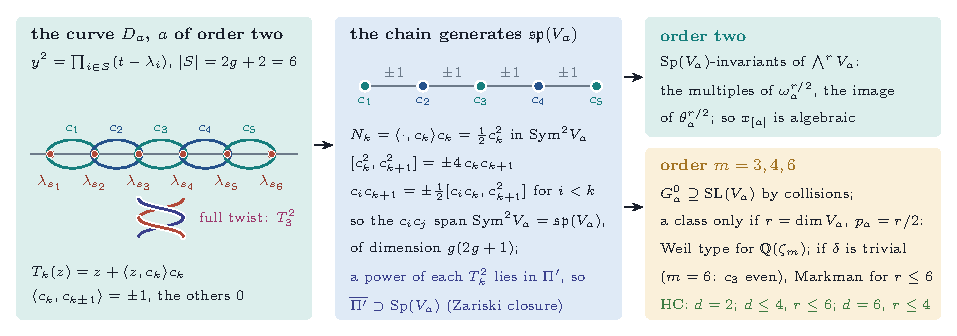
\includegraphics[width=\textwidth]{fig_vgmonodromy}
\caption{The proof of \Cref{thm:vgvandermonde}. Left: the hyperelliptic
curve $D_{a}$ of a character of order two, drawn over the six points of its
support for $g=2$, with the chain of vanishing cycles $c_{1},\dots,c_{5}$;
a full twist of two neighbouring branch points, drawn as a braid, acts by
the square of the transvection $T_{k}$. Middle: the chain as a graph, and the
induction in $\mathrm{Sym}^{2}V_{a}$ by which the logarithms $N_{k}$ generate
$\mathfrak{sp}(V_{a})$. Right: what the monodromy leaves of the Hodge
classes, the powers of the polarisation for characters of order two, and
for characters of order three, four and six the Weil classes of an abelian
variety of Weil type for $\QQ(\sqrt{-3})$ or $\QQ(i)$.}
\label{fig:vgmonodromy}
\end{figure}

\Cref{fig:vgmonodromy} draws the steps of the proof. The dimensions of (iii)
never exceed $h^{r/2,r/2}(X)$, and they equal it for a quadric, for
the Fermat hypersurfaces (for cubics $7$, $21$ and $71$ in dimensions $2$, $4$
and $6$, for quartics $142$ and $1108$ in dimensions $4$ and $6$, for sextics
$1752$ in dimension $4$) and for two quadrics in $\PP^{N}$ with $N$ even
($N+2$), where every class of type $(r/2,r/2)$ is algebraic. For two cubics
in $\PP^{6}$ the very general member has $141$ Hodge classes of degree four
against $h^{2,2}=267$, and for three quartics in $\PP^{7}$ it has $3950$
against $h^{2,2}=29872$ (\Cref{fig:vgcounts}). \Cref{fig:vgscope} shows, for each degree $d$ and dimension $r$,
what is known for the very general member.

\begin{figure}[tbp]
\centering
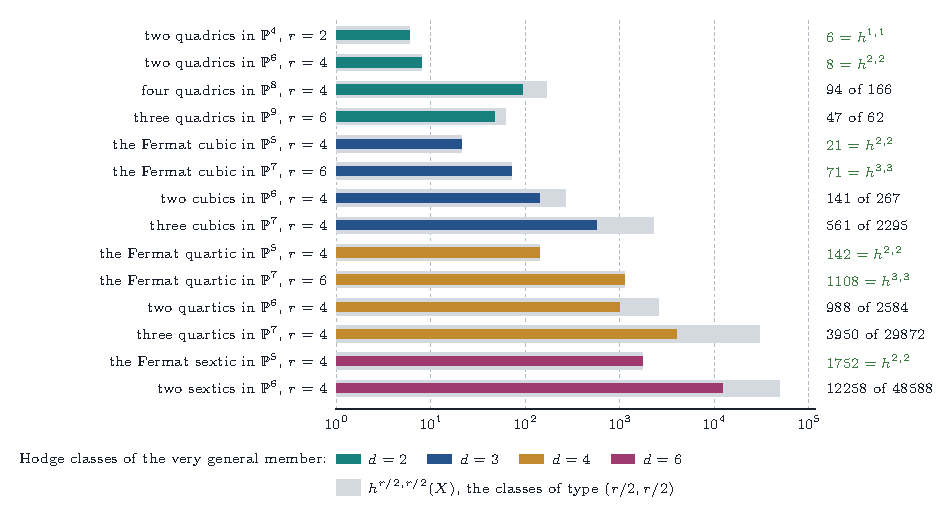
\includegraphics[width=\textwidth]{fig_vgcounts}
\caption{The dimension of the space of Hodge classes of degree $r$ on the
very general member, from \Cref{thm:vgvandermonde}(iii), against the Hodge
number $h^{r/2,r/2}$, on a logarithmic scale. Where the two agree, the
space $H^{r/2,r/2}$ is spanned by Hodge classes at every configuration;
elsewhere the very general member has fewer Hodge classes, and the members
with more lie over a countable union of proper closed subsets of the space
of configurations.}
\label{fig:vgcounts}
\end{figure}

\begin{figure}[tbp]
\centering
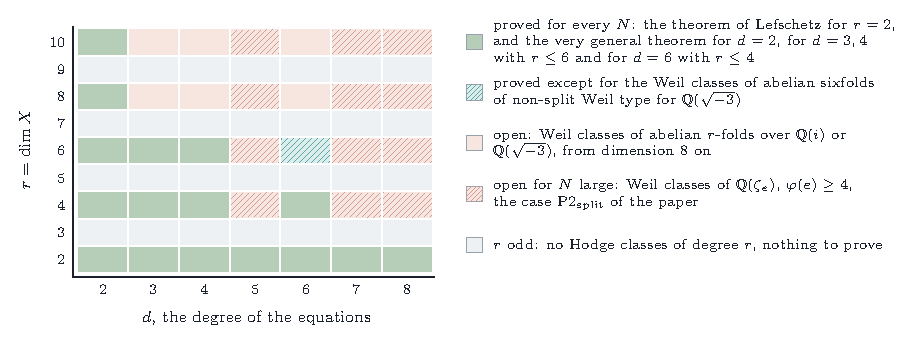
\includegraphics[width=\textwidth]{fig_vgscope}
\caption{The Hodge conjecture for the very general complete intersection
$X_{d,r}(\lambda)$ of Vandermonde type, for every $N$. Grass: proved, by the
theorem of Lefschetz for $r=2$ and by \Cref{thm:vgvandermonde} for $d=2$,
for $d=3,4$ with $r\le6$ and for $d=6$ with $r\le4$. Teal hatching: proved
except for the Weil classes of abelian sixfolds of non-split Weil type for
$\QQ(\sqrt{-3})$. Clay: open, the Weil classes of abelian varieties of Weil
type over $\QQ(i)$ or $\QQ(\sqrt{-3})$ in dimension at least eight, or,
hatched, of a CM field of degree at least four (\Cref{rem:vandermonde}).
For odd $r$ there is nothing to prove.}
\label{fig:vgscope}
\end{figure}

\begin{remark}[What the diagonal complete intersections give]
\label{rem:vandermonde}
\Cref{thm:vandermonde} adds to the domain of \textup{(F3$'$)} a family of
complete intersections of every dimension and every degree, parametrised by
configurations of $N+1$ points on the line, among them all smooth complete intersections of two diagonal
hypersurfaces; for $c\ge3$ and $r\ge2$ the condition on the columns is a real
restriction. \Cref{cor:twodiagonal} shows on them how \textup{(F3$'$)} and
(F2) together give the conjecture: once the Hodge classes of $X$ are
carried to the abelian varieties $B_{[a]}$, the conjecture for $X$ is the
algebraicity of their Hodge classes, a question of type (F2), and for the
fourfolds in $\PP^{6}$ of degrees $3$, $4$ and $6$ it is answered by
Markman's theorem: their exceptional classes are Weil classes of abelian
fourfolds of Weil type, $490$ families of them for $d=4$. For $d=3$ these
fourfolds are Fano and the conjecture also follows from the theorem of Conte
and Murre on uniruled fourfolds \cite{CM78}; for $d=4$ and $d=6$ they are of
general type, with $h^{2,2}=2584$ and $48588$. Complete intersections of
diagonal hypersurfaces, and of quadrics, are also the subject of Terasoma's
paper \cite{Ter88}. At a very general configuration
\Cref{thm:vgvandermonde} goes further, in every $\PP^{N}$: for $d=2$ in every
dimension, for $d=3$ and $d=4$ up to dimension seven, and for $d=6$ up to
dimension five, through the monodromy of cyclic covers of degree three, four
and six (\Cref{prop:cyclicmonodromy}). For $d=3$ and $r\ge8$ the
conjecture for the very general member is the algebraicity of the Weil
classes of the abelian $r$-folds $B_{[a]}$ of split Weil type for
$\QQ(\sqrt{-3})$, which is open from dimension eight on, and the same holds
for $d=4$ with $\QQ(i)$. For $d=6$ and $r=6$ the open classes are those of
the abelian sixfolds of non-split Weil type for $\QQ(\sqrt{-3})$ of
\Cref{thm:vgvandermonde}(iii), such as the one of the character
$(1,1,2,2,3,5,5,5)$ on eight points. Beyond these cases the
same reduction meets (F2) itself: for $d=5$ or $d\ge7$ and $N$ large enough, some
$B_{[a]}$ with $\dim V_{a}=r$ carries an action of $\QQ(\zeta_{e})$, $e\mid d$,
with $\varphi(e)\ge4$, and $W_{[a]}$ is the top exterior power of its first
cohomology over that CM field, which consists of Hodge classes when the
types are balanced: Weil classes for a CM field of degree at least four, of
the kind treated in \cite[Theorem~1.1]{paperI}; and for larger $N$ the $B_{[a]}$ have
dimension above five.
\end{remark}

\begin{remark}[Where \textup{(F3$'$)} stops]\label{rem:f3primefrontier}
With \Cref{prop:f3prime}, \Cref{prop:aclosure} and \Cref{prop:f3primesmall},
\textup{(F3$'$)} holds on every variety of dimension at most three, on every
fourfold whose zero-cycles are supported in dimension three (in particular
every uniruled fourfold), on every fivefold whose zero-cycles are supported
in dimension at most three, on every fourfold and fivefold whose maximal
rationally connected quotient is birational to a variety satisfying
\textup{(F3$'$)} in degree four (\Cref{prop:f3primefibration}), on every
fourfold and fivefold dominated by a rational map from such a variety
(\Cref{prop:f3primedominant}), and on
every member of $\mathcal{A}$, a class containing the Fermat
hypersurfaces, the smooth Delsarte hypersurfaces with the cyclic covers
branched along them (\Cref{cor:delsarteall}), and the complete intersections
of diagonal hypersurfaces of Vandermonde type, among them every smooth
complete intersection of two diagonal hypersurfaces (\Cref{thm:vandermonde},
\Cref{cor:twodiagonal}), of every degree and dimension, the Hilbert schemes of points on
abelian surfaces, on products of curves and on the K3 surfaces of
\Cref{prop:aclosure}(iv), the generalised Kummer varieties $K_{n}(A)$ and the
other varieties of \Cref{prop:aclosure}(v), and every blow-up and projective bundle
built from these. Through the Hodge conjecture itself it holds on the
complete intersections of \Cref{cor:twodiagonal}(ii), among them the
fourfolds of general type cut out by two diagonal quartics or sextics in
$\PP^{6}$, on the very general complete intersections of diagonal quadrics,
of diagonal cubics and quartics up to dimension seven and of diagonal
sextics up to dimension five, of \Cref{thm:vgvandermonde}, and on the
varieties of \Cref{prop:k3powers}, \Cref{prop:k3ntype} and
\Cref{cor:fanolines}: for a K3 surface $S$ with
$E=\End_{\mathrm{Hdg}}(T(S))$ a CM field, on every power, Hilbert scheme and
moduli space of $S$; for $E=\QQ$ and $t=\dim T(S)$, on $S^{k}$ for $k<t$, on
$S^{[n]}$ for $n<t(t+1)/2$ and on the moduli spaces of dimension less than
$t$; on every fourfold of K3$^{[2]}$ type whose field $E$ is $\QQ$ or a CM
field; on $F(Y)$ and $Y\times Y$ for every cubic fourfold $Y$ with such a
field; and on every fourfold of generalised Kummer type \cite{FV25}. Its
frontier cases are these (\Cref{fig:f3primereach}), the first two in
degree four on fourfolds whose zero-cycles are not supported on a proper
closed subset and which are not birational to a member of $\mathcal{A}$ by
any construction above: $S\times S$ and $S^{[2]}$ for a K3 surface
whose real multiplication is not induced by a cycle constructed so far, such
as $S_{\lambda}$
(the known cases are recalled in \Cref{rem:mumfordks}); the fourfolds of
K3$^{[2]}$ type with real multiplication, among them $F(Y)$ for a cubic
fourfold $Y$ with real multiplication, and with it $Y\times Y$; and, for a
very general K3 surface, the single class $\det T(S)$ on $S^{21}$ of
\Cref{prop:orthpowers}, equivalently the Hodge conjecture for $S^{[231]}$.
In the first two the
rational Hodge isometries \cite{Bus19,Mar24} act on $T$ by $\pm1$, and a
composite of Hodge similarities that returns to $T$ is an element $g\in E$
with $g^{2}\in\QQ$, the adjoint involution of $E$ being trivial; such
elements span only the compositum of the quadratic subfields of $E$, which is
$\QQ$ for the cubic field of $S_{\lambda}$. Apart from proving the
conjecture itself where zero-cycles are small, none of these results touches
the step that
\Cref{rem:f3primeopen} identifies: putting a Hodge class into
$\mathrm{Ab}^{p}(X)$ for a variety that no correspondence connects to an
abelian variety. \Cref{thm:closure} is unchanged, since every statement
proved here is a special case of one of the hypotheses of its rule set, not a
new rule.
\end{remark}

\begin{figure}[tbp]
\centering
  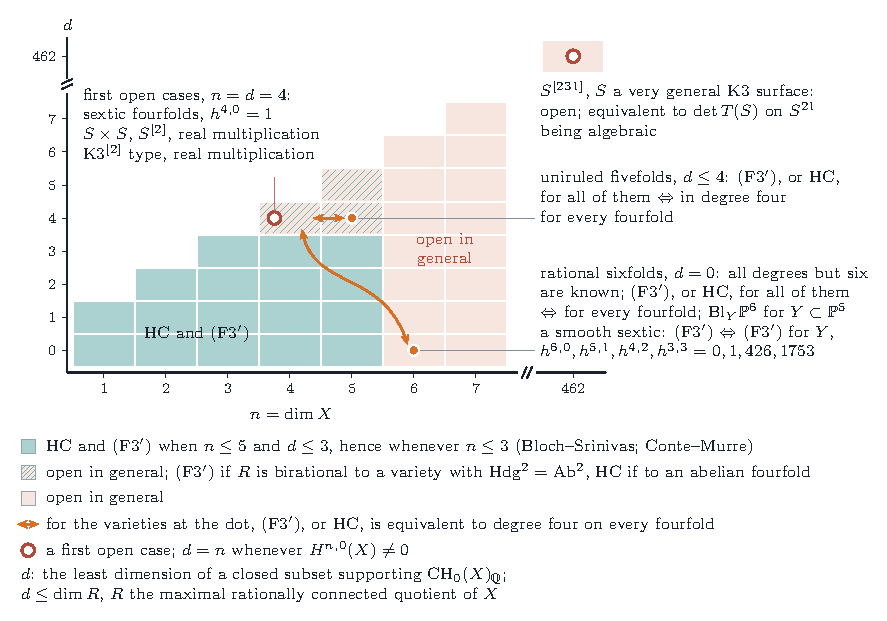
\includegraphics[width=\textwidth]{fig_f3primereach}
\caption{What arguments on zero-cycles and on rationally connected
fibrations give for \textup{(F3$'$)} and for the Hodge conjecture (HC in the
figure) on a variety $X$, over the plane of $n=\dim X$ and the least dimension
$d$ of a closed subset supporting $\mathrm{CH}_{0}(X)_{\QQ}$; $d$ is at most
the dimension of the maximal rationally connected quotient $R$ of $X$, and
$d=n$ whenever $H^{n,0}(X)\ne0$ (\Cref{rem:f3primesharp}). Both hold when
$n\le5$ and $d\le3$ (\Cref{prop:f3primesmall}), hence on every variety of
dimension at most three. In the hatched cells
\textup{(F3$'$)} holds when $R$ is birational to a variety with
$\Hdg^{2}=\mathrm{Ab}^{2}$, for instance a member of $\mathcal{A}$, and the
Hodge conjecture when $R$ is birational to an abelian fourfold
(\Cref{prop:f3primefibration}). The double arrows are the equivalences of
\Cref{rem:f3primesharp}: \textup{(F3$'$)}, and the Hodge conjecture, hold for
every uniruled fivefold, and for every rational sixfold, if and only if they
hold in degree four for every fourfold; the sixfold $\mathrm{Bl}_{Y}\PP^{6}$
of a smooth sextic fourfold $Y$ in a hyperplane carries the Hodge numbers
listed. The rings are the frontier cases (\Cref{rem:f3primefrontier}): the
sextic fourfolds, the first family of smooth hypersurfaces beyond these
results
(the $29$ Delsarte sextics lie in $\mathcal{A}$ by
\Cref{cor:delsarteall}); $S\times S$ and $S^{[2]}$ for a K3
surface $S$ with real multiplication, such as
$S_{\lambda}$; the fourfolds of K3$^{[2]}$ type with real multiplication,
among them $F(Y)$; and, beyond the breaks of the axes, $S^{[231]}$ for a very
general K3 surface, which is equivalent to the algebraicity of $\det T(S)$ on
$S^{21}$ (\Cref{prop:k3powers}, \Cref{fig:k3threshold}).}
\label{fig:f3primereach}
\end{figure}

\begin{setupenv}[The rule set]\label{setup:rules}
The rule set has forty-two statements and twenty-two rules. Ten statements
are proved in this paper: the base point with an explicit cycle in every Weil
family of an imaginary quadratic field (\cite[Theorem~15.27]{paperI}) and of a CM
field of degree at least four (\cite[Theorem~17.5]{paperI}); for each of the two
kinds of field, the reduction of the Weil classes of a family to one class at
every point of one connected domain, and the stability of the algebraic locus
under the rational points, with dense orbits (\cite[Section~12]{paperI},
\cite[Proposition~16.7]{paperI}, \cite[Theorem~17.7]{paperI}); and four statements on
secant objects: the form of the weakened criterion for the transform
(\cite[Theorem~4.56]{paperII}), the conditions of Markman's strategy that bear on the
Chern character, the description of the local obstruction as a failure of
Cohen--Macaulayness (\cite[Corollary~4.77]{paperII}), and three of the four
ingredients of the construction in every dimension. Four are quoted:
$\mathbf{W}(K,2,\delta)$ for every $K$ and $\delta$, $\mathbf{W}(K,3,\delta_{0})$
\cite{Mar25a,Mar25b}, the deformation theorem for motivated classes
\cite[Th\'eor\`eme~0.5]{And96b}, and the accessibility of Hodge classes on
abelian varieties \cite[\S5.1, Theorem~3]{Mil20}. Sixteen are hypotheses:
(F3), (F2) of \Cref{cor:fourremain} and (F3$'$) of \Cref{def:f3prime};
(L), (M), (V) of \Cref{def:lmv}; (P2), in the polarised form of
\cite[Remark~3.6]{paperII}, for four groups of families, the split and the other
families of the imaginary quadratic fields and of the CM fields of degree at
least four, the third group giving $\mathrm{P2}_{\mathrm{split}}$; secant
objects meeting the weakened criterion in every dimension, and an affirmative
answer to \cite[Question~11.4]{Mar25b}; and, for a smooth and for a singular
Cohen--Macaulay support on an abelian fourfold, its existence with the
required extension property and the vanishing of the image of the product of
translation classes. The other twelve are derived: $\mathbf{HC}$, the
conjecture for every abelian variety, written $\mathbf{AB}$, and the Weil
classes of every CM field, of the imaginary quadratic fields, of their
families of trivial and of nontrivial discriminant, of the CM fields of
degree at least four and of their split and their other families, together
with one secant object on an abelian fourfold, $\mathbf{W}(K,4,\delta_{0})$,
and the range settled in the literature. Each rule is a finite set of
premises with one conclusion, and each is a theorem of this paper:
\Cref{tab:rules} lists twenty-one of them, and the twenty-second derives the
range settled in the literature from the two quoted Weil statements. For a
set $T$ of statements write $\Cn(T)$ for the least set that contains $T$ and
is closed under the rules, which exists because each rule has a single
conclusion and the consequence operator is therefore monotone. Write
$\mathbf{T}$ for the set of statements proved or quoted. Call a set $S$ of
hypotheses \emph{sufficient} if $\mathbf{HC}\in\Cn(\mathbf{T}\cup S)$, and
\emph{minimal} if no proper subset of $S$ is sufficient.
\end{setupenv}

\begin{table}[htbp]
\centering
\small
\renewcommand{\arraystretch}{1.14}
\begin{tabular}{@{}>{\raggedright\arraybackslash}p{0.40\linewidth}>{\raggedright\arraybackslash}p{0.27\linewidth}l@{}}
\toprule
premises & conclusion & by \\
\midrule
the conjecture for abelian varieties, (F3)
  & $\mathbf{HC}$ & \Cref{ssec:closuremap} \\
(F3)
  & abelian varieties & \Cref{prop:f3ishc} \\
the conjecture for abelian varieties, (F3$'$)
  & $\mathbf{HC}$ & \Cref{prop:f3prime} \\
the Weil classes of every CM field, (F2)
  & abelian varieties & \Cref{ssec:closuremap} \\
$K$ imaginary quadratic, the fields of degree at least four
  & every CM field & \cite[Appendix~C]{paperI} \\
$\delta=\delta_{0}$, $\delta\ne\delta_{0}$
  & every discriminant & \Cref{prop:separate} \\
a base point, the reduction, the orbit, (P2) for the family
  & that family & \cite[Theorem~2.3]{paperII} \\
the same three for a CM field of degree at least four, (P2) for the family
  & that family & \cite[Theorem~17.7]{paperI} \\
its split families, its other families
  & the fields of degree at least four & \cite[Proposition~17.3]{paperI} \\
$\delta=\delta_{0}$
  & $\delta\ne\delta_{0}$ & \Cref{prop:descent} \\
the split families of the fields of degree at least four
  & their other families; $\delta=\delta_{0}$ & \Cref{prop:descent} \\
a secant object in every dimension, Question 11.4
  & $\delta=\delta_{0}$ & \cite[Proposition~15.19]{paperI} \\
a Cohen--Macaulay support, smooth or singular
  & one secant object & \cite[Corollary~4.77]{paperII} \\
one secant object, Question 11.4
  & $\mathbf{W}(K,4,\delta_{0})$ & \cite[Corollary~4.57]{paperII} \\
\midrule
(L), (M)
  & $\mathbf{HC}$ & \Cref{prop:lefmot} \\
(L), the deformation theorem for motivated classes
  & (V) & \Cref{prop:lefvhc} \\
(V), the accessibility of Hodge classes on abelian varieties
  & abelian varieties & \Cref{thm:vhcab} \\
\bottomrule
\end{tabular}
\caption{The rules of \Cref{setup:rules} whose conclusion is derived, with the
theorem that proves each; the rows for (P2) and for the Cohen--Macaulay
support each stand for two rules, the row for descent over the fields of
degree at least four for two, descent within a field and scalar extension
down to the imaginary quadratic fields, the second row is \Cref{prop:f3ishc},
the third is
\Cref{prop:f3prime}(i) for the weaker statement (F3$'$) of
\Cref{def:f3prime}, the last three rows are the rules of
\Cref{ssec:bullseye}, one of whose conclusions, (V), is itself a
hypothesis of the rule set, and the one remaining rule records what the literature supplies on Weil classes. The
bounded criterion (P1) is absent: by
\cite[Theorem~16.17]{paperI} it is equivalent to its own conclusion, so it is a
restatement and not a premise.}
\label{tab:rules}
\end{table}

\begin{theorem}[The closure of what is proved here]\label{thm:closure}
With the notation of \Cref{setup:rules}:
\begin{enumerate}[label=\textup{(\roman*)},leftmargin=2.6em]
\item $\mathbf{HC}\notin\Cn(\mathbf{T})$. Nothing in this paper, combined with the
  theorems it quotes, implies the Hodge conjecture.
\item There are exactly five minimal sufficient sets:
  \[
    \{\mathrm{F3}\},\quad\{\mathrm{L},\mathrm{M}\},\quad
    \{\mathrm{L},\mathrm{F3}'\},\quad\{\mathrm{V},\mathrm{F3}'\},\quad
    \{\mathrm{P2}_{\mathrm{split}},\mathrm{F2},\mathrm{F3}'\},
  \]
  with \textup{(L)}, \textup{(M)}, \textup{(V)} as in \Cref{def:lmv},
  \textup{(F2)}, \textup{(F3)} as in \Cref{cor:fourremain}, (F3$'$) as in
  \Cref{def:f3prime}, and $\mathrm{P2}_{\mathrm{split}}$ the propagation
  statement \textup{(P2)}, read in the polarised form of \cite[Remark~3.6]{paperII},
  for the split families of the CM fields of degree at least four. No
  minimal set contains \textup{(P2)} for an imaginary quadratic field or for
  a family of nontrivial discriminant: \Cref{prop:descent} derives those.
  The single hypothesis (F3) is sufficient, and it is equivalent to
  $\mathbf{HC}$ (\Cref{prop:f3ishc}); no other single hypothesis is.
  The sets $\{\mathrm{L},\mathrm{F3}\}$, $\{\mathrm{V},\mathrm{F3}\}$ and
  $\{\mathrm{P2}_{\mathrm{split}},\mathrm{F2},\mathrm{F3}\}$ are sufficient and
  not minimal. The last of the five is the only one with three elements and the
  only one whose derivation of $\mathbf{HC}$ uses a statement proved in this
  paper.
\item In each of the five, every element is necessary: removing any one
  leaves $\mathbf{HC}$ outside the closure.
\item The secant route lies in no minimal sufficient set. Granting both of its
  demands, a secant object satisfying the weakened criterion in every
  dimension and an affirmative answer to \cite[Question 11.4]{Mar25b}, puts
  $\mathbf{W}(K,n,\delta_{0})$ in the closure, and with it, by
  \Cref{prop:descent}, $\mathbf{W}(K,n,\delta)$ for every $\delta$; it leaves
  the Weil classes of the CM fields of degree at least four outside.
\item No statement proved in this paper rests, at any depth, on a
  hypothesis, and the rule set is acyclic.
\item Every element of a minimal sufficient set other than
  $\mathrm{P2}_{\mathrm{split}}$ is a consequence of $\mathbf{HC}$, and $\{\mathrm{F3}\}$ and
  $\{\mathrm{L},\mathrm{M}\}$ are each equivalent to it; no implication from
  $\mathbf{HC}$ to \textup{(P2)} is known.
\end{enumerate}
\end{theorem}

\begin{proof}
(i) and (v). No rule has a proved or quoted statement as its conclusion, so
each of them lies in $\Cn(\mathbf{T})$ by itself, on the strength of its proof
in this paper or in the literature; this is the first assertion of (v). The
twenty-second rule is the only one whose premises all lie in $\mathbf{T}$:
every other rule has among its premises a hypothesis or a derived statement
other than the range settled in the literature. Hence $\Cn(\mathbf{T})$ is
$\mathbf{T}$ together with that range, and it does not contain $\mathbf{HC}$,
which is (i). For acyclicity, list first the thirty statements that are
proved, quoted or hypotheses other than (V); then one secant object,
$\mathbf{W}(K,4,\delta_{0})$ and the range settled in the literature; the
split and then the other families of the CM fields of degree at least four;
the families of trivial and then of nontrivial discriminant of the imaginary
quadratic fields; the imaginary quadratic fields, the CM fields of degree at
least four and every CM field; and last (V), $\mathbf{AB}$ and $\mathbf{HC}$.
The premises of every rule come before its conclusion in this list.

(ii) and (iii). The five sets are sufficient:
$\mathrm{F3}\Rightarrow\mathbf{AB}$ (\Cref{prop:f3ishc}) and
$\mathbf{AB}\wedge\mathrm{F3}\Rightarrow\mathbf{HC}$; $\mathrm{L}\wedge
\mathrm{M}\Rightarrow\mathbf{HC}$ (\Cref{prop:lefmot}); (L) and the
deformation theorem give (V) (\Cref{prop:lefvhc}), (V) and accessibility give
$\mathbf{AB}$ (\Cref{thm:vhcab}), and $\mathbf{AB}\wedge\mathrm{F3}'
\Rightarrow\mathbf{HC}$ (\Cref{prop:f3prime}(i)), which settles
$\{\mathrm{L},\mathrm{F3}'\}$ and $\{\mathrm{V},\mathrm{F3}'\}$; and
$\mathrm{P2}_{\mathrm{split}}$ with the CM base point, the reduction and the
orbit gives the split families of the CM fields of degree at least four
(\cite[Theorem~17.7]{paperI}), descent gives their other families and the
families of trivial discriminant of the imaginary quadratic fields
(\Cref{prop:descent}), hence the fields of degree at least four
(\cite[Proposition~17.3]{paperI}), the nontrivial discriminant (\Cref{prop:descent}),
the imaginary quadratic fields (\Cref{prop:separate}) and every CM field
(\cite[Appendix~C]{paperI}), and with (F2) this is $\mathbf{AB}$ and with (F3$'$)
it is $\mathbf{HC}$.

Let $C_{1}$, respectively $C_{2}$, be the set of all statements other than
$\mathbf{HC}$, (F3), (F3$'$) and (L), respectively (M). Let $C_{3}$ be the
set of all statements other than $\mathbf{HC}$, $\mathbf{AB}$, the Weil
classes of every CM field, of the fields of degree at least four and of their
split families, (F3), (L), (V) and $\mathrm{P2}_{\mathrm{split}}$; and let
$C_{4}$ be the set of all statements other than $\mathbf{HC}$,
$\mathbf{AB}$, (F3), (L), (V) and (F2). Each $C_{j}$ contains $\mathbf{T}$
and not $\mathbf{HC}$, and each is closed under the rules: every rule whose
conclusion it omits has a premise it omits. For $C_{1}$ and $C_{2}$ the only
omitted conclusion is $\mathbf{HC}$, and the three rules with that
conclusion have the premises (F3), (F3$'$), and (L) and (M). For $C_{3}$
and $C_{4}$ the rules with conclusion $\mathbf{HC}$ have the premises
$\mathbf{AB}$ or (L); those with conclusion $\mathbf{AB}$ have the premises
(F3), the Weil classes of every CM field together with (F2), and (V); the
only rule with conclusion (V) has the premise (L); and for $C_{3}$ the rule
for every CM field needs the fields of degree at least four, the rule for
these needs their split families, and the rule for the split families needs
$\mathrm{P2}_{\mathrm{split}}$. Since $\Cn$ is monotone, a set of
hypotheses contained in some $C_{j}$ has its closure, together with
$\mathbf{T}$, inside $C_{j}$, and is not sufficient. So a sufficient set
meets each of
\begin{gather*}
  H_{1}=\{\mathrm{F3},\mathrm{F3}',\mathrm{L}\},\qquad
  H_{2}=\{\mathrm{F3},\mathrm{F3}',\mathrm{M}\},\\
  H_{3}=\{\mathrm{F3},\mathrm{L},\mathrm{V},\mathrm{P2}_{\mathrm{split}}\},\qquad
  H_{4}=\{\mathrm{F3},\mathrm{L},\mathrm{V},\mathrm{F2}\},
\end{gather*}
the hypotheses omitted from $C_{1},\dots,C_{4}$. Let $S$ meet all four. If
$\mathrm{F3}\in S$, then $S\supseteq\{\mathrm{F3}\}$. If $\mathrm{F3}\notin S$
and $\mathrm{L}\in S$, then $S$ meets $H_{2}$ in (F3$'$) or (M). If neither is
in $S$, then $S$ contains (F3$'$), from $H_{1}$, and (V) or both
$\mathrm{P2}_{\mathrm{split}}$ and (F2), from $H_{3}$ and $H_{4}$. So a set
of hypotheses is sufficient exactly when it contains one of the five sets,
and as none of the five contains another, they are the minimal sufficient
sets. The other assertions of (ii) can be read off the list, and the
derivations above show that only the last uses a statement proved here;
(iii) is the minimality.

(iv) Granting the two demands of the secant route, the rule of
\cite[Proposition~15.19]{paperI} gives the families of trivial discriminant, descent
those of nontrivial discriminant, and \Cref{prop:separate} the imaginary
quadratic fields. The set formed by $\mathbf{T}$, the range settled in the
literature, the two demands and these three statements is closed, since
every other rule has a premise outside it: a hypothesis not granted, one
secant object, or a Weil statement about the fields of degree at least four
or about every CM field. Every base point the secant route produces is a
member $X\times\widehat{X}$, whose discriminant is trivial whatever $\beta$
is chosen (\cite[Proposition~15.19(ii)]{paperI}); the deformation argument stays inside
the family of trivial discriminant, and it is \Cref{prop:descent}(i), not
the deformation, that carries the result to the other discriminants. The
route has no base point over a field of degree at least four, so it reaches
none of them, and none of its hypotheses lies in one of the five sets.

(vi) \textup{(L)} follows from $\mathbf{HC}$ by \cite[Theorem~12.2]{paperI},
\textup{(M)} by \Cref{prop:lefmot}, \textup{(V)} by \Cref{prop:lefvhc},
(F3$'$) by \Cref{prop:f3prime}(i), and (F2) and (F3) are special cases of
$\mathbf{HC}$. The equivalence of $\{\mathrm{F3}\}$ with $\mathbf{HC}$ is
\Cref{prop:f3ishc}, and $\{\mathrm{L},\mathrm{M}\}$ is equivalent to it by
\Cref{prop:lefmot} and the first two implications.
\end{proof}

\begin{corollary}[The three statements, one of which is the
conjecture]\label{cor:fourremain}
The Hodge conjecture follows from the results of this paper together with the
following three statements. No rule of \Cref{setup:rules} derives it from
(F1) and (F2) together, and it follows from (F3) alone, which is equivalent
to it
(\Cref{prop:f3ishc}); so the list is not a reduction of the conjecture to
three smaller problems. With (F3) replaced by the weaker statement
\textup{(F3$'$)} of \Cref{def:f3prime}, the conjecture modulo abelian
varieties, the three statements (F1), (F2), \textup{(F3$'$)} still suffice,
and no rule of \Cref{setup:rules} derives the conjecture from a proper
subset of them. With the rule of \Cref{prop:f2isab}, which the rule set does
not contain, (F2) and \textup{(F3$'$)} already suffice (\Cref{rem:f2rule}).
\begin{enumerate}[label=\textup{(F\arabic*)},leftmargin=3.0em,itemsep=4pt]
\item \emph{One propagation statement, for every CM field.} \textup{(P2)},
  in the polarised form of \cite[Remark~3.6]{paperII}: at one base point of each
  Weil family of each CM field some perfect complex whose Chern character is
  a nonzero multiple of a rational Weil class plus a polynomial in the
  polarisation has injective semiregularity map. Its first form, with Chern
  character exactly a multiple of the Weil class, is false for every
  imaginary quadratic field and every $n\ge2$ (\cite[Theorem~3.5]{paperII}): such a
  complex would have to deform to non-algebraic Weil tori, whose coherent
  sheaves have no Chern character in degrees $1$ to $2n-1$. The polarised form
  closes
  $\mathbf{W}(K,n,\delta)$
  for every imaginary quadratic $K$, every $n$ and every $\delta$ at once, by
  \cite[Theorem~2.3]{paperII}, and
  $\mathbf{W}(F,n,\delta)$ for every CM field $F$ of higher degree, by
  \cite[Theorem~17.7]{paperI}, because those theorems put $\Sigma=\cD$, so the
  Weil class is algebraic at every member of the family and not only at the
  general one, and because \cite[Theorem~15.27]{paperI} and \cite[Theorem~17.5]{paperI}
  supply the base point in every one of those families. By
  \Cref{prop:descent} it is enough to have it for the split families of the
  CM fields of degree at least four, in infinitely many dimensions.
  \cite[Theorem~2.5]{paperII}, \cite[Theorem~2.13]{paperII}, \Cref{thm:nosum},
  \cite[Theorem~2.11]{paperII} and \cite[Theorem~2.14]{paperII} describe the object of the
  first form and are vacuous by \cite[Theorem~3.5]{paperII}; for the polarised form
  \cite[Theorem~3.9]{paperII} computes the number that $\dim\Ext^{2}(E,E)$ has
  to reach, $7n^{2}-2n$ for a general shape. For one family its
  conclusion is equivalent to the Lefschetz standard conjecture for one
  variety (\Cref{cor:weilequiv}). The bounded criterion \textup{(P1)} is not a
  second form of the same demand: by
  \cite[Theorem~16.17]{paperI} it is equivalent to the conclusion it was to imply,
  and \cite[Theorem~16.15]{paperI} shows that the one cycle it could have been tested
  on, the transport of the base cycle, does not satisfy it.
\item \emph{The classes beyond the Weil lines.} Every Hodge class on an
  abelian variety that lies outside the subring generated by divisor classes
  and by Weil classes of quotients is algebraic. Through dimension five there
  is no such class \cite{MZ99}; in dimension eight there are
  (\Cref{prop:mumfordproduct}), so this is not a reduction of the conjecture
  for abelian varieties to Weil classes, which is false as a statement about
  Hodge rings: it is the conjecture for those classes, and by
  \Cref{prop:f2isab} it is equivalent to the conjecture for every abelian
  variety. Its smallest case is
  brought down to one Kuga--Satake class in \Cref{thm:mumfordks}; it holds at
  every CM point (\Cref{thm:mumfordcm}), and on all members of a Mumford
  family it is equivalent to the Lefschetz standard conjecture for one
  ninefold (\Cref{cor:mumfordequiv}). Its classes are rigid along the base
  curve (\Cref{thm:mumfordrigid}), and one complex at one CM point with
  $\Ext^{2}$ of dimension $119$ would close it (\Cref{thm:mumfordnumerical}),
  as would a bound on the cycles that represent them at the closed points of
  the reductions of the curve modulo primes (\Cref{thm:modpdensity}).
\item \emph{The varieties that are not abelian.} The Hodge conjecture holds
  for every smooth complex projective variety that is not an abelian variety.
  This is the Hodge conjecture itself. The varieties it covers include
  $A\times\PP^{1}$ for every abelian variety $A$, and the conjecture for
  $A\times\PP^{1}$ gives it for $A$ (\Cref{prop:f3ishc}); so (F3) implies
  the conjecture for abelian varieties, hence (F1) and (F2), and hence
  $\mathbf{HC}$. Nor is it a reduction to abelian varieties in the other
  direction: no realisation of the cohomology of an arbitrary variety inside
  that of abelian varieties exists (\Cref{prop:noabeliantype}), and
  \cite[Theorem~10.3]{paperI} and \cite[Theorem~10.8]{paperI} close the two routes
  through hyperplane sections that would be the natural candidates for one.
\end{enumerate}
\end{corollary}

\begin{proof}
The three together are sufficient by the derivation of \Cref{thm:closure},
and (F3) alone by \Cref{prop:f3ishc}. That (F1) and (F2) together are not
sufficient in the rule set is \Cref{thm:closure}(ii), since every minimal
sufficient set contains (F3), \textup{(F3$'$)} or \textup{(M)}; the
statement about (F1), (F2), \textup{(F3$'$)} is \Cref{thm:closure}(ii) and
(iii) for the last of the five minimal sets. The Weil classes of the CM
fields of degree at least four are not a fourth statement: they are derived
from (F1) by \cite[Theorem~17.7]{paperI}. Nor is the bounded criterion a
premise, since by \cite[Theorem~16.17]{paperI} it is a restatement of its own
conclusion.
\end{proof}

\begin{remark}[Necessity relative to a rule set, and the wording of (F2)]
\label{rem:f3collapse}
A rule set can show that a set of statements suffices; it can show that a set
is needed only relative to the implications written into it. A rule set that
used (F3) only through $\text{(abelian varieties)}\wedge
\text{(F3)}\Rightarrow\mathbf{HC}$, without the elementary rule
$\text{(F3)}\Rightarrow\text{(abelian varieties)}$ of \Cref{prop:f3ishc},
would make the three statements of \Cref{cor:fourremain} look jointly
necessary, although (F3) alone suffices.

The wording of (F2) has the same feature, one degree at a time. Let
$R(A)\subseteq H^{*}(A,\QQ)$ be the subring generated by divisor classes and
Weil classes of quotients. Suppose some Hodge class $\beta$ of degree $2p$ on
$A$ lies outside $R(A)$, and let $\alpha$ be any Hodge class of degree $2p$.
If $\alpha\notin R(A)$, (F2) makes it algebraic. If $\alpha\in R(A)$, then
$\alpha+\beta\notin R(A)$, because $R(A)$ is closed under subtraction, so
(F2) makes $\alpha+\beta$ and $\beta$ algebraic, and with them $\alpha$.
So in every degree in which (F2) says anything it is the whole conjecture for
that degree: on the square of a Mumford fourfold it gives every Hodge class of
$H^{4}$, the six products of divisor classes included. Multiplying by an
exceptional class of that square moves every Hodge class of every abelian
variety outside the subring, and \Cref{prop:f2isab} deduces from this that
(F2) is the whole conjecture for abelian varieties. The rule set does not
contain that implication; \Cref{rem:f2rule} says how \Cref{thm:closure}(ii)
changes when it is adjoined.

The form of (F3) that is not the conjecture itself asks only for
algebraicity modulo classes coming from abelian varieties. It is
\textup{(F3$'$)} of \Cref{def:f3prime}; \Cref{prop:f3prime} says what is
known of it, and \Cref{rem:f3primeopen} why it is not closed.
\end{remark}

\begin{figure}[tbp]
\centering
  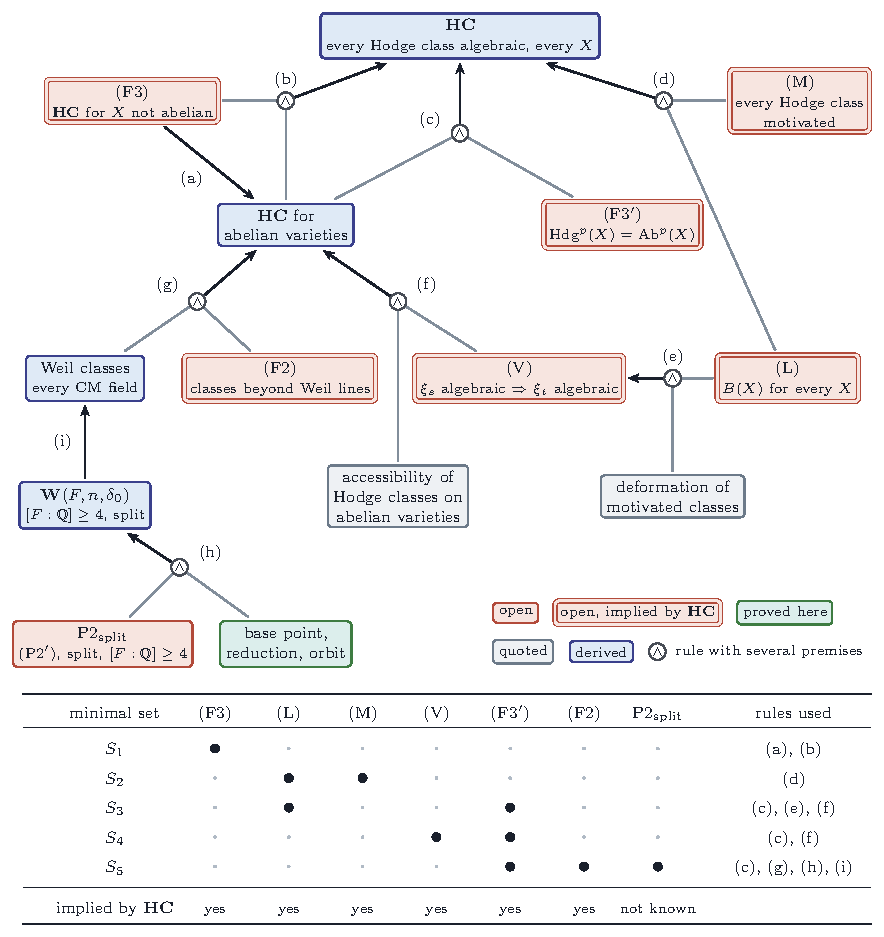
\includegraphics[width=0.92\textwidth]{fig_frontier}
\caption{The rule set of \Cref{setup:rules} with the rules of
\Cref{ssec:bullseye}, drawn as a hypergraph. A rule with several premises is
a junction marked $\wedge$, joined to its premises and with one arrow to its
conclusion. The letters name the results that prove the rules: (a) is
\Cref{prop:f3ishc}; (b) and (g) are the closure map of
\Cref{ssec:closuremap}; (c) is \Cref{prop:f3prime}(i); (d) is
\Cref{prop:lefmot}; (e) is \Cref{prop:lefvhc}; (f) is \Cref{thm:vhcab};
(h) is \cite[Theorem~17.7]{paperI}; and (i) is the chain of
\Cref{prop:descent}, \Cref{prop:separate}, \cite[Proposition~17.3]{paperI} and
\cite[Appendix~C]{paperI}. Clay marks a hypothesis, a double frame a hypothesis
that the conjecture implies, grass what this paper proves, slate
what it quotes, and indigo a derived statement. The table lists the five
minimal sufficient sets of \Cref{thm:closure}(ii), the rules each of them
uses, and which of the hypotheses the conjecture implies; only
$\mathrm{P2}_{\mathrm{split}}$, which asks for a particular complex, is
drawn without that frame. The secant route, which reaches the imaginary
quadratic families only, is drawn in \Cref{fig:closure}.}
\label{fig:frontier}
\end{figure}

\begin{remark}[The target, and what it would take]\label{rem:bullseye}
With the rules of \Cref{ssec:bullseye}, \Cref{prop:f3ishc} and
\Cref{prop:f3prime} in place, \Cref{thm:closure} changes the reading of
\Cref{cor:fourremain} in three ways. First, the route through this paper is
a route only with (F3) replaced by \textup{(F3$'$)}. As stated, its last
statement (F3) is the conjecture (\Cref{prop:f3ishc}), so (F1) and (F2), and
everything this paper proves about Weil classes, drop out of every minimal
derivation that uses (F3). With \textup{(F3$'$)} in its place the route
$\{\mathrm{P2}_{\mathrm{split}},\mathrm{F2},\mathrm{F3}'\}$ is minimal, and it is not the
shortest: (F1) and (F2), which between them give the conjecture for abelian
varieties along this route, are replaced on the routes of the literature by
the single statement \textup{(V)} (\Cref{thm:vhcab}), or by \textup{(L)},
which implies it (\Cref{prop:lefvhc}). Second, every element of every minimal sufficient set
except $\mathrm{P2}_{\mathrm{split}}$ is a consequence of the conjecture
(\Cref{thm:closure}(vi)), and
two of the sets, $\{\mathrm{F3}\}$ and $\{\mathrm{L},\mathrm{M}\}$, are
each equivalent to it. (P2) is a statement about semiregularity maps, and a
proof of the conjecture need not prove it; in its first form, with a Chern
character that is exactly a Weil class, it is false (\cite[Theorem~3.5]{paperII}), and
the route runs through the polarised form of \cite[Remark~3.6]{paperII}. Third, every minimal sufficient set
contains (F3), \textup{(F3$'$)} or \textup{(M)}: the varieties that are not
abelian are reached only through the conjecture for them, which is the whole
conjecture, through the conjecture modulo abelian varieties
(\Cref{rem:f3primeopen}), or through motivated classes.

So the target at the centre is \textup{(L)}. It lies in two of the five
minimal sets, it gives \textup{(V)} and with it the whole abelian half, the
conjecture implies it, and with \textup{(M)} it is the conjecture. For each
$X$ it asks for one explicit Hodge class on $X\times X$ to be algebraic, the
class inducing $\Lambda$. This paper proves \textup{(L)}, \textup{(M)},
\textup{(V)} and \textup{(F3$'$)} on the classes of varieties named here:
\Cref{cor:mumfordlefschetz} adds the total spaces of Mumford families to the
known cases of \textup{(L)}, \Cref{prop:f3prime} records the known cases of
\textup{(F3$'$)}, and the routes of the literature use no other theorem of
this paper.
\end{remark}

\subsubsection*{Two of the three are not reductions}

One could hope that (F2) and (F3) are reductions in the ordinary sense,
statements to the effect that every Hodge class is carried, by some
correspondence, to a class on a Weil type variety or on an abelian variety,
so that the whole conjecture would follow from the Weil classes alone. Both
hopes are refutable, and we refute them, because a frontier that contains a
false statement is not a frontier.

\begin{proposition}[The Hodge ring is not generated by divisor and Weil
classes]\label{prop:mumfordproduct}
Let $X$ be a complex abelian fourfold whose Hodge group is a $\QQ$-form of an
almost direct product of three copies of $\mathrm{SL}_{2}$, acting on
$V=H^{1}(X,\QQ)$ through the tensor product $V_{1}\otimes V_{2}\otimes V_{3}$
of the three standard representations, with $\End^{0}(X)=\QQ$; such
fourfolds exist and form families of dimension one, by Mumford
\cite{Mum69}, and by \cite[2.5(i)]{MZ99} they are exactly the fourfolds
with $\End^{0}(X)=\QQ$ and Hodge group smaller than $\Sp_{8}$. Then:
\begin{enumerate}[label=\textup{(\roman*)},nosep,leftmargin=2.6em]
\item the Hodge ring of $X$ is generated by the polarisation:
  $\dim_{\QQ}\Hdg^{1}(X)=\dim_{\QQ}\Hdg^{2}(X)=1$;
\item $\dim_{\QQ}\Hdg^{1}(X\times X)=3$ and $\dim_{\QQ}\Hdg^{2}(X\times X)=8$,
  while the products of divisor classes span a subspace of dimension $6$
  in $H^{4}(X\times X,\QQ)$;
\item the two remaining classes lie in $H^{4}(X\times X,\QQ)$ and are Weil
  classes of no CM field acting on $X\times X$, on a quotient of it, or on an
  abelian subvariety of it.
\end{enumerate}
In particular the statement that every Hodge class on an abelian variety
lies in the subring generated by divisor classes and Weil classes of
quotients is false in dimension eight, though true through dimension five
\cite{MZ99}.
\end{proposition}

\begin{proof}
Hodge classes are the invariants of the Hodge group, so
$\Hdg^{k}(Y)\otimes\CC$ is the space of $\Hg(Y)_{\CC}$-invariants in
$\bigwedge^{2k}H^{1}(Y,\CC)$, and $\Hg(X\times X)=\Hg(X)$ acting
diagonally on $V\oplus V$. Over $\CC$ the group is
$\mathrm{SL}_{2}^{3}$ and the weights of $V$ under its maximal torus are the
eight sign vectors $(\pm1,\pm1,\pm1)$. Write $V=V_{1}\otimes W$ with
$W=V_{2}\otimes V_{3}$, on which $\mathrm{SL}_{2}^{2}=\mathrm{Spin}(4)$ acts
orthogonally. The Cauchy formula
$\bigwedge^{k}(V_{1}\otimes W)=\bigoplus_{|\lambda|=k}S_{\lambda}V_{1}\otimes
S_{\lambda'}W$ \cite[\S6.1]{FH91}, with $S^{2}V_{1}=S_{(3,1)}V_{1}=V(2)$,
$\bigwedge^{2}V_{1}=S_{(2,2)}V_{1}=\mathbf{1}$ and $S^{4}V_{1}=V(4)$, gives
$\bigwedge^{2}V=V(2)\otimes\bigwedge^{2}W\oplus S^{2}W$ and
$\bigwedge^{4}V=V(4)\otimes\bigwedge^{4}W\oplus V(2)\otimes S_{(2,1,1)}W
\oplus S_{(2,2)}W$. Under $\mathrm{Spin}(4)$, $\bigwedge^{2}W=V(2,0)\oplus
V(0,2)$, $S^{2}W=V(2,2)\oplus\mathbf{1}$, $\bigwedge^{4}W=\mathbf{1}$,
$S_{(2,1,1)}W\cong\mathfrak{sl}(W)=\bigwedge^{2}W\oplus S^{2}_{0}W$, and
$S_{(2,2)}W=V(4,0)\oplus V(0,4)\oplus V(2,2)\oplus\mathbf{1}$, the
decomposition of the algebraic curvature tensors in dimension four into the
self-dual and anti-self-dual Weyl parts, the traceless Ricci part and the
scalar part. Hence
\begin{gather*}
  \textstyle\bigwedge^{2}V=V(2,2,0)\oplus V(2,0,2)\oplus V(0,2,2)\oplus\mathbf{1},\\
  \textstyle\bigwedge^{4}V=V(2,2,2)\oplus\bigoplus_{\text{cyc}}V(4,0,0)
  \oplus\bigoplus_{\text{cyc}}V(2,2,0)\oplus\mathbf{1},
\end{gather*}
each with one trivial summand, which is (i). For (ii),
$\bigwedge^{4}(V\oplus V)=\bigoplus_{a}\bigwedge^{a}V\otimes\bigwedge^{4-a}V$
and the invariants in $\bigwedge^{a}V\otimes\bigwedge^{4-a}V$ are
$\Hom_{\mathrm{SL}_{2}^{3}}(\bigwedge^{a}V,\bigwedge^{4-a}V)$, since every
summand is self-dual; the counts are $1,1,4,1,1$, total $8$, the $4$ coming
from the four distinct irreducible summands of $\bigwedge^{2}V$. Likewise the
invariants in $\bigwedge^{2}(V\oplus V)$ number $1+1+1=3$. The divisor
classes of $X\times X$ are the three symplectic forms $\psi_{11}$, $\psi_{12}$,
$\psi_{22}$ on $V\oplus V$ built from the polarisation $\psi$ of $V$. Their
six pairwise products are linearly independent: they lie in the summands
$\bigwedge^{a}V\otimes\bigwedge^{4-a}V$ with $a=4,3,2,2,1,0$, each is
nonzero, and in the summand $a=2$ the classes $\psi_{11}\psi_{22}$ and
$\psi_{12}^{2}$ correspond, as maps $\bigwedge^{2}V\to\bigwedge^{2}V$, to a
multiple of the projection onto $\CC\psi$ and to a multiple of the
identity. The $\Sp_{8}$-invariants of $\bigwedge^{4}(V\oplus V)$ number
$1+1+2+1+1=6$ by the same count, since $\bigwedge^{1}V=V$,
$\bigwedge^{2}V=\bigwedge^{2}_{0}V\oplus\mathbf{1}$ and
$\bigwedge^{3}V=\bigwedge^{3}_{0}V\oplus V$ under $\Sp_{8}$; so the six
products are all the classes a Hodge group equal to $\Sp_{8}$ would allow. For (iii), the Weil classes of an abelian
variety $Y$ with respect to a CM field $F\subseteq\End^{0}(Y)$ are, by
definition, the classes in $\bigwedge^{2k}_{F}H^{1}(Y,\QQ)\subseteq
H^{2k}(Y,\QQ)$ with $2k=\dim_{F}H^{1}(Y,\QQ)$ (\cite[Setup~17.1]{paperI}). A CM
field acting on $X\times X$ lies in $\End^{0}(X\times X)=M_{2}(\QQ)$, so it is
imaginary quadratic, $2k=8$, and its Weil classes lie in $H^{8}$, while the two
classes of (ii) have degree four. Every proper
abelian subvariety and every proper quotient of $X\times X$ is isogenous to
$X$, because $X$ is simple, and $\End^{0}(X)=\QQ$ contains no CM field, so $X$
carries no Weil classes at all. This is the statement of \cite[0.1(iii)]{MZ99}
that the exceptional classes of $X\times X$ are not of Weil type. The last
sentence is (ii) and (iii) together with the theorem of \cite{MZ99} for
dimension at most five.
\end{proof}

\begin{proposition}[No Hodge-theoretic reduction to abelian varieties]
\label{prop:noabeliantype}
Let $Y$ be a very general smooth quintic threefold in $\PP^{4}$, and let
$V=H^{3}(Y,\QQ)$ with its polarised Hodge structure of weight three. Then $V$
is not isomorphic to a subquotient of any Hodge structure of the form
$\bigoplus_{i}T_{i}$, where each $T_{i}$ is obtained from the $H^{1}$ of
finitely many abelian varieties by tensor products, duals and Tate twists. In
particular the Hodge structure $H^{*}(Y,\QQ)$ is not of abelian type, and no
correspondence between $Y$ and an abelian variety, or a product of abelian
varieties, induces an injection of $V$ into the cohomology of the latter.
\end{proposition}

\begin{proof}
Write $\mathrm{MT}(W)$ for the Mumford--Tate group of a rational Hodge
structure $W$ and $\mu_{W}\colon\mathbb{G}_{m}\to\mathrm{MT}(W)_{\CC}$ for
its Hodge cocharacter, acting on $W^{p,q}$ by $z^{p}$. The adjoint action of
$\mu_{W}$ on $\operatorname{Lie}\mathrm{MT}(W)_{\CC}\subseteq\End(W_{\CC})$ has weights
among the differences $p-p'$ of two Hodge indices of $W$.

If $W$ has weight one, these differences lie in $\{-1,0,1\}$. If $W'$ is a
subquotient of a tensor construction $T$ on $W$, then $\mathrm{MT}(W')$ is the
image of $\mathrm{MT}(W)$ acting on $W'$, and $\mu_{W'}$ is the image of
$\mu_{W}$; so $\operatorname{Lie}\mathrm{MT}(W')$ is a quotient of $\operatorname{Lie}\mathrm{MT}(W)$
as a representation of $\mathbb{G}_{m}$ through $\mu$, and its weights are a
subset of $\{-1,0,1\}$. The same holds with $W=\bigoplus H^{1}(A_{i})$.
Hence for every Hodge structure of abelian type the adjoint weights of the
Hodge cocharacter lie in $\{-1,0,1\}$.

For $V=H^{3}(Y,\QQ)$ we show that the adjoint weight $3$ occurs. The
canonical bundle of a quintic threefold is trivial by adjunction, so
$h^{3,0}(Y)=1$; pick $0\ne e\in H^{3,0}$. The intersection form $\psi$ on $V$
is symplectic and pairs $H^{3,0}$ with $H^{0,3}$ perfectly, so the rank one
endomorphism $x\mapsto\psi(x,e)\,e$ of $V_{\CC}$ is nonzero, sends $H^{0,3}$
to $H^{3,0}$ and kills the rest, and lies in $\mathfrak{sp}(V_{\CC},\psi)$
because $\psi(\psi(x,e)e,y)+\psi(x,\psi(y,e)e)
=\psi(x,e)\bigl(\psi(e,y)+\psi(y,e)\bigr)=0$; its adjoint weight is
$3-0=3$. It remains to see that $\mathfrak{sp}(V_{\CC},\psi)\subseteq
\operatorname{Lie}\mathrm{MT}(V)_{\CC}$. Let $S$ be the parameter space of smooth quintic
threefolds, connected and nonsingular, and $\mathbb{V}$ the polarisable
variation of Hodge structure $R^{3}$ of the universal family. The connected
algebraic monodromy group $G^{0}$ of $\mathbb{V}$ contains the connected
monodromy group of any Lefschetz pencil of quintics, that is of hyperplane
sections of the fifth Veronese image of $\PP^{4}$; for a Lefschetz pencil of
odd fibre dimension the image of the monodromy representation on the
$\ell$-adic vanishing cohomology $E\otimes\QQ_{\ell}$ is open in
$\Sp(E\otimes\QQ_{\ell},\psi)$ \cite[Theorem 5.10]{Del74}, so the Zariski
closure of the monodromy group over $\QQ$ is $\Sp(E,\psi)$; here
$E=H^{3}(Y_{t},\QQ)$, the vanishing cohomology being the orthogonal
complement of the image of $H^{3}(\PP^{4},\QQ)=0$. Hence $G^{0}\supseteq
\Sp(V,\psi)$, and $G^{0}\subseteq\Sp(V,\psi)$ since the monodromy preserves
$\psi$. At a very general
point $Y$ the group $G^{0}$ is a normal subgroup of the derived group of
$\mathrm{MT}(V)$ \cite[Theorem 1]{And92}, so $\Sp(V,\psi)\subseteq
\mathrm{MT}(V)^{\mathrm{der}}\subseteq\Sp(V,\psi)$, and the adjoint weight
$3$ occurs in $\operatorname{Lie}\mathrm{MT}(V)$. So $V$ is not of abelian type, and
neither is any Hodge structure containing it as a subquotient, in particular
$H^{*}(Y,\QQ)$. A correspondence inducing an injection of $V$ into the
cohomology of an abelian variety would exhibit $V$ as a sub-Hodge structure
of a Tate twist of that cohomology, which is of abelian type.
\end{proof}

\begin{figure}[tbp]
\centering
  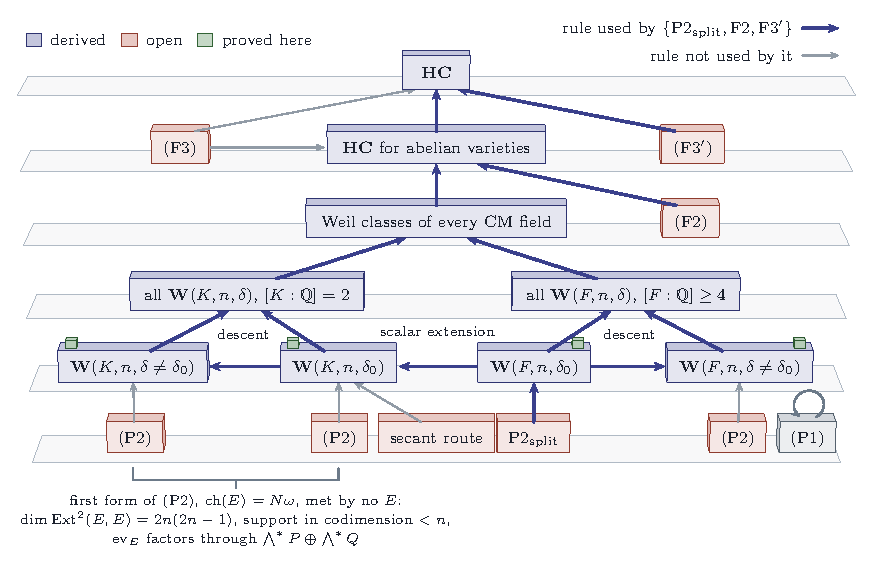
\includegraphics[width=\textwidth]{fig_closure}
\caption{The route of this paper through the rule set of \Cref{thm:closure},
drawn as a stack of plates, one per level of the derivation; the other routes
are drawn in \Cref{fig:frontier}. Heavy arrows are the rules used by the
minimal set $\{\mathrm{P2}_{\mathrm{split}},\mathrm{F2},\mathrm{F3}'\}$,
light arrows the rules it does not use. The bottom plate carries the
propagation statement, read in the polarised form of \cite[Remark~3.6]{paperII},
once for each of the four kinds of Weil family, with the secant route beside
it. The small grass blocks on the next plate are the base points of
\cite[Theorem~15.27]{paperI} and \cite[Theorem~17.5]{paperI}, one in every family. The
three arrows inside that plate are \Cref{prop:descent}: descent from the
trivial discriminant to the others, and scalar extension from the fields of
degree at least four to the quadratic fields. With them (P2) is needed only
for the split families of the fields of higher degree, and the other three
(P2) blocks are not used. (F2) is the conjecture for the Hodge classes that
no Weil line reaches, and (F3) is the whole conjecture
(\Cref{prop:f3ishc}), so the route is minimal only with (F3) replaced by
\textup{(F3$'$)} of \Cref{def:f3prime}. The bracket under the two quadratic
(P2) blocks records the first form of the criterion, in which the Chern
character is exactly a Weil class, as \cite[Theorem~2.11]{paperII},
\cite[Theorem~2.13]{paperII} and \cite[Corollary~2.9]{paperII} describe it; by
\cite[Theorem~3.5]{paperII} that form is met by no complex. The secant route reaches
the trivial discriminant, since the member it is built on is split, and
through descent the rest of the quadratic case; it has no edge to the fields
of higher degree. The bounded criterion (P1) stands apart, closed on itself:
it is equivalent to its own conclusion.}
\label{fig:closure}
\end{figure}


\subsection{Routes from outside algebraic geometry}\label{ssec:outside}

By \Cref{prop:f2isab} and \Cref{prop:f3prime}(i), the two statements
\textup{(F2)} and \textup{(F3$'$)} are the two halves of the conjecture: the
conjecture for abelian varieties, and the conjecture modulo abelian varieties.
A route from another domain must therefore either produce algebraic cycles or
arrive at one of the hypotheses of \Cref{setup:rules}. This subsection
records what the routes most often proposed do. One of them, the analytic
route through positive currents, can be made exact: the conjecture is the
vanishing of an integrality gap in a mass minimisation problem whose real
version is solved, and positivity, which is what analysis sees first, cannot
distinguish an algebraic class from any other.

Throughout, $X$ is a smooth complex projective variety of dimension $n$, $h\in
H^{2}(X,\ZZ)$ is the class of an ample line bundle, $\omega_{h}$ is a K\"ahler
form with class $h$, and for $c\in H^{2p}(X,\QQ)$ we put
\[
  L_{h}(c)=\int_{X}c\cup\frac{h^{\,n-p}}{(n-p)!}\in\QQ .
\]
A real $(p,p)$-form is \emph{strongly positive} if at every point it is a
nonnegative combination of forms $\mathrm{i}\beta_{1}\wedge\bbar{\beta}_{1}
\wedge\cdots\wedge\mathrm{i}\beta_{p}\wedge\bbar{\beta}_{p}$ with $\beta_{j}$
of type $(1,0)$; the closed positive currents of bidegree $(p,p)$ are the
currents nonnegative on such forms of the complementary degree, and every
smooth closed strongly positive form is one \cite[Chapter~III]{Dem12}.

\begin{proposition}[Positivity is no test]\label{prop:positivitynotest}
For every class $\alpha\in H^{p,p}(X,\RR)$, $0\le p\le n$, there is an integer
$N$ such that $\alpha+Nh^{p}$ is the class of a smooth closed strongly positive
$(p,p)$-form. Consequently every real $(p,p)$-class becomes the class of a
closed positive current after the addition of a multiple of $h^{p}$, and, since
$h^{p}$ is algebraic, a Hodge class is algebraic if and only if the positive
class $\alpha+Nh^{p}$ is: no property of a class implied by positivity, or by
its being a limit of classes of effective cycles, separates the algebraic Hodge
classes from the others.
\end{proposition}

\begin{proof}
Let $V=T_{x}X$ with the hermitian form $\omega_{h}(x)$, and let
$\mathrm{SP}_{p}\subseteq\Lambda^{p,p}_{\RR}V^{\vee}$ be the closed convex cone
generated by the forms $\mathrm{i}^{p}\beta_{1}\wedge\bbar{\beta}_{1}\wedge\cdots
\wedge\beta_{p}\wedge\bbar{\beta}_{p}$. These forms span
$\Lambda^{p,p}_{\RR}V^{\vee}$, so $\mathrm{SP}_{p}$ has nonempty interior, and
$\omega_{h}(x)^{p}$ lies in that interior: in a unitary basis $dz_{1},\dots,
dz_{n}$ of $V^{\vee}$,
\[
  \omega_{h}^{p}=p!\sum_{|J|=p}\Bigl(\frac{\mathrm{i}}{2}\Bigr)^{p}
  dz_{J}\wedge d\bbar{z}_{J},
\]
and a generator $D=\mathrm{i}^{p}\beta_{1}\wedge\bbar{\beta}_{1}\wedge\cdots\wedge
\beta_{p}\wedge\bbar{\beta}_{p}$ equals $|\det B|^{2}\,2^{p}(\mathrm{i}/2)^{p}
dz_{1}\wedge d\bbar{z}_{1}\wedge\cdots\wedge dz_{p}\wedge d\bbar{z}_{p}$ after a
unitary change of coordinates taking the span of the $\beta_{j}$ to that of
$dz_{1},\dots,dz_{p}$, with $B$ the matrix of the $\beta_{j}$ in that basis;
so $\omega_{h}^{p}-\delta D\in\mathrm{SP}_{p}$ for $0<\delta\le p!/(2^{p}
|\det B|^{2})$. As every real $(p,p)$-form is a finite real combination of
generators, $\omega_{h}^{p}+\varepsilon\gamma\in\mathrm{SP}_{p}$ for every
$\gamma$ and all small $\varepsilon$, which is interiority. The cone, the form
$\omega_{h}(x)^{p}$ and the norm defined by $\omega_{h}(x)$ are carried into
each other by unitary frames, so the radius $r>0$ of a ball around
$\omega_{h}(x)^{p}$ contained in $\mathrm{SP}_{p}$ does not depend on $x$.
Represent $\alpha$ by a smooth closed real $(p,p)$-form $a$, for instance its
harmonic representative, and let $N\ge\max_{X}|a|/r$. Then
$a+N\omega_{h}^{p}=N(\omega_{h}^{p}+a/N)$ is strongly positive at every point,
closed, and represents $\alpha+Nh^{p}$. The remaining assertions follow, the
last because a class of the form $\alpha+Nh^{p}$ is positive for every $\alpha$.
\end{proof}

The proposition says what positivity cannot do. Demailly studied the cone of
closed positive currents against the conjecture and constructed extremal
closed strongly positive currents that are not integration currents on
analytic sets \cite{Dem82}, so extremality does not single out the algebraic
cycles either. What positivity can do is turn the conjecture into a
variational statement, and the statement is exact. It is the K\"ahler case of
a formulation that Harvey and Lawson give for every calibrated manifold
\cite[Section~6, Proposition~6.13 and Remarks~6.9 and~6.11]{HL09}; we state
it for the classes of this paper, with the effective representative that
\Cref{lem:cibig} supplies, and then apply it to the Mumford square. For a
closed integral current $T$ of dimension $2(n-p)$ on $X$, Wirtinger's
inequality \cite[1.8.2]{Fed69}, \cite{HK74}, \cite[II.3]{HL82} gives
\begin{equation}\label{eq:wirtinger}
  \mathbf{M}(T)\;\ge\;T\Bigl(\frac{\omega_{h}^{\,n-p}}{(n-p)!}\Bigr)
  \;=\;L_{h}(c),
\end{equation}
where $\mathbf{M}$ is the mass and $c\in H^{2p}(X,\ZZ)$ is the Poincar\'e dual
of the homology class of $T$, with equality if and only if the approximate
tangent plane of $T$ is a complex subspace, positively oriented, at
$\|T\|$-almost every point. The right side depends on $c$ alone.

\begin{lemma}[Complete intersection classes are big]\label{lem:cibig}
For every algebraic class $\beta\in H^{2p}(X,\QQ)$ there is an integer $M$ such
that $\beta+Mh^{p}$ is a positive rational combination of classes of
irreducible subvarieties of codimension $p$; so some positive integer multiple
of $\beta+Mh^{p}$ is the class of an effective algebraic cycle.
\end{lemma}

\begin{proof}
Replacing $h$ by a multiple, which changes $M$, we may assume $h$ very ample.
Let $Z\subseteq X$ be irreducible of codimension $p$, and let $d$ be such that
the ideal sheaf $I_{Z}(d)$ is globally generated. The base locus of the linear
system of divisors of degree $d$ containing $Z$ is exactly $Z$, so by Bertini
$p$ general members $D_{1},\dots,D_{p}$ of it meet properly away from $Z$.
Every component of $D_{1}\cap\cdots\cap D_{p}$ has codimension at most $p$;
a component not contained in $Z$ has codimension exactly $p$, because the
$D_{i}$ meet properly off $Z$, and a component contained in $Z$ has
codimension at least $p$ and so equals $Z$. The intersection is therefore the
union of $Z$ and a closed set $W'$ of pure codimension $p$. Hence $d^{p}h^{p}=[D_{1}]\cdots[D_{p}]=m[Z]+[W']$ with $m\ge1$ and
$W'$ effective \cite[Chapter~7]{Ful98}, and $h^{p}-\varepsilon[Z]$ is an
effective rational class for $0<\varepsilon\le m/d^{p}$. Write
$\beta=\sum_{i}n_{i}[Z_{i}]$ with $n_{i}\in\QQ$ and choose $\varepsilon_{i}$ for
each $Z_{i}$ with $n_{i}<0$; then for $M\ge\sum_{n_{i}<0}|n_{i}|/\varepsilon_{i}$
the class $\beta+Mh^{p}$ is $\sum_{n_{i}>0}n_{i}[Z_{i}]+\sum_{n_{i}<0}
(|n_{i}|/\varepsilon_{i})(h^{p}-\varepsilon_{i}[Z_{i}])+(M-\sum_{n_{i}<0}
|n_{i}|/\varepsilon_{i})h^{p}$, a positive rational combination of effective
classes, $h^{p}$ itself being the class of a complete intersection.
\end{proof}

\begin{theorem}[The conjecture as a mass gap]\label{thm:massgap}
Let $\alpha\in\Hdg^{p}(X)$ be a rational Hodge class.
\begin{enumerate}[label=\textup{(\roman*)},leftmargin=2.6em,itemsep=2pt]
\item Let $N\ge1$ be an integer with $N\alpha$ integral, let $M$ be an
  integer for which $\alpha+Mh^{p}$ is the class of a smooth closed strongly
  positive form, as every large $M$ is by \Cref{prop:positivitynotest}, and
  put $c=N(\alpha+Mh^{p})$. The minimum of the mass over closed real normal
  currents of dimension $2(n-p)$ in the class dual to $c$ is $L_{h}(c)$, and
  it is attained by a smooth strongly positive form. The minimum over closed
  integral currents in the same class exists and is at least $L_{h}(c)$.
\item The class $\alpha$ is algebraic if and only if there are integers
  $N\ge1$ and $M\ge0$, with $N\alpha$ integral, for which the minimum of the
  mass over closed integral currents in the class dual to $N(\alpha+Mh^{p})$
  equals $L_{h}(N(\alpha+Mh^{p}))$; and then every mass minimising integral
  current in that class is the integration current of an effective algebraic
  cycle.
\item Write $\|c\|_{\ZZ}$ for the minimum in \textup{(i)} over integral
  currents. By a theorem of Federer, recorded in this form by Harvey and
  Lawson \cite[Section~6]{HL09}, \cite{Fed69,Fed74}, $\lim_{k\to\infty}
  \|kc\|_{\ZZ}/k=L_{h}(c)$: the integrality gap closes asymptotically for
  every class. The class $\alpha$ is algebraic if and only if, for every
  sufficiently large $M$, the gap is closed at some finite $k$, that is,
  $\|kc\|_{\ZZ}=kL_{h}(c)$ for some $k\ge1$.
\end{enumerate}
In particular the conjecture for $X$ is the statement that for every rational
Hodge class the integrality gap of this problem vanishes for some $N$ and $M$;
\textup{(F2)} is that statement for abelian varieties. Teh and Yang give a
different sufficient condition in the same setting, through Lipschitz chains
that are closed for $d$ and $d^{c}$ with positive $(k,k)$-part
\cite[Theorem~4.2]{TY21}.
\end{theorem}

\begin{proof}
(i) The form $\omega_{h}^{n-p}/(n-p)!$ has comass one and calibrates exactly
the complex $2(n-p)$-planes, which is Wirtinger's inequality
\cite[1.8.2]{Fed69}; so every closed real normal current $S$ in the class has
$\mathbf{M}(S)\ge S(\omega_{h}^{n-p}/(n-p)!)=L_{h}(c)$. By
\Cref{prop:positivitynotest} the class is represented by a smooth closed
strongly positive form $a$, and for a strongly positive $(p,p)$-form the mass of
the current it defines is $\int_{X}a\wedge\omega_{h}^{n-p}/(n-p)!$, because a
strongly positive $2(n-p)$-vector is a nonnegative combination of complex unit
planes, each of mass one and calibrated. So the minimum over real currents is
$L_{h}(c)$ and $a$ attains it. Closed normal currents represent every real
homology class and closed integral currents every integral one
\cite[5.11]{FF60}, and by the compactness theorem of Federer and Fleming the
mass attains its minimum on the closed integral currents in a given class
\cite[9.6]{FF60}; the lower bound is \eqref{eq:wirtinger}.

(ii) If $\alpha$ is algebraic, \Cref{lem:cibig} gives $M$ and $N$ with
$N(\alpha+Mh^{p})=\sum_{j}n_{j}[V_{j}]$, $n_{j}\in\ZZ_{>0}$, $V_{j}$
irreducible of codimension $p$. The integration current $T=\sum_{j}n_{j}[V_{j}]$
is a closed locally integral current \cite[Theorem~3.1.1]{Kin71}, its tangent
planes are complex and positively oriented, so equality holds in
\eqref{eq:wirtinger} and $\mathbf{M}(T)=L_{h}(c)$ with $c=N(\alpha+Mh^{p})$.
Conversely let $T$ be a closed integral current in the class dual to $c$ with
$\mathbf{M}(T)=L_{h}(c)$, for instance a mass minimiser when the minimum is
$L_{h}(c)$. Equality in \eqref{eq:wirtinger} makes $T$ a closed locally
rectifiable current of bidimension $(n-p,n-p)$ which is positive, and by
King's theorem \cite[Theorem~5.2.1]{Kin71} such a current is a holomorphic
cycle $\sum_{j}n_{j}[V_{j}]$ with $n_{j}$ nonzero integers and $V_{j}$
irreducible analytic subvarieties of dimension $n-p$; positivity makes every
$n_{j}$ positive. (Harvey and Shiffman characterised the holomorphic chains
among closed rectifiable currents of bidimension $(n-p,n-p)$ without
positivity, under a hypothesis on the support that Alexander removed
\cite{HS74,Ale97}.) By Chow's theorem \cite[p.~167]{GH78} the $V_{j}$
are algebraic, so $c$ is the class of an effective algebraic cycle and $\alpha$
is algebraic. This is the argument of \cite[Proposition~6.13]{HL09}.

(iii) The limit is Federer's theorem on the real and integral masses of a
class, as stated in the final note of \cite[Section~6]{HL09}; with (i) the
limit is $L_{h}(c)$, since the real minimum is attained by a smooth form. If
the gap is closed at $k$, then (ii), applied with $kN$ in place of $N$, makes
$\alpha$ algebraic. Conversely, if $\alpha$ is algebraic, \Cref{lem:cibig}
gives $M_{0}$ such that $\alpha+M_{0}h^{p}$ is a positive rational
combination of classes of subvarieties; for $M\ge M_{0}$ so is
$\alpha+Mh^{p}$, since $h^{p}$ is the class of a complete intersection, and
some multiple $kc$ is the class of an effective cycle, whose integration
current attains the bound. For a fixed small $M$ the equivalence is not asserted, since it would
need an effective multiple of every algebraic class represented by a
strongly positive form, in codimension at least two. The last sentence of the
theorem is the definition of the conjecture for $X$, and \Cref{prop:f2isab}
for \textup{(F2)}.
\end{proof}

\begin{example}[The Mumford square]\label{ex:mumfordmass}
Let $Y=X\times X$ be the square of a Mumford fourfold at a very general point
of its curve, with the product principal polarisation $\theta_{Y}$, and let
$\omega$ be one of the two exceptional classes of \Cref{prop:mumfordproduct},
normalised in $H^{2}(X)\otimes H^{2}(X)$ with $a_{0}=0$ in the notation of
\Cref{setup:omegaa}, so that it corresponds to an endomorphism of $H^{2}(X)$
killing $\theta$ with image in the primitive part. Then
$L_{\theta_{Y}}(\omega)=0$: the pairing of $\omega$ with
$\theta_{Y}^{6}=\sum_{k}\binom6k\theta^{k}\otimes\theta^{6-k}$ sees only the
term $20\,\theta^{3}\otimes\theta^{3}$, and $\int_{X}x\cup\theta^{3}=0$ for
every primitive $x\in H^{2}(X)$. Also $L_{\theta_{Y}}(\theta_{Y}^{2})=8!/6!=56$,
and $4\theta_{Y}^{2}$ is the class of the complete intersection $D\cap D'$ of two
general members of $|2\theta_{Y}|$, a base point free system, whose integration
current has mass $224$. By \Cref{thm:massgap} and \Cref{cor:mumfordone}, the
Hodge conjecture for every member of the Mumford family, and with it
$B(W\times_{C}W)$, is equivalent to the following: for some integers
$N\ge1$ and $M\ge1$ with $N\omega$ integral, the class dual to
$N(M\theta_{Y}^{2}+\omega)$ contains an integral current of mass exactly
$56NM$; and any such current is an effective algebraic cycle representing the
class. For $M$ divisible by four the class $NM\theta_{Y}^{2}$ contains one,
$NM/4$ copies of $D\cap D'$, of mass $56NM$; so the question is whether the
perturbation by $N\omega$, which changes the Wirtinger bound by nothing, can
be absorbed without mass. By \Cref{thm:mumfordcm} the answer is yes at
every CM point of the curve, with integers $N$ and $M$ depending on the
point; and if the same $N$ and $M$ served at infinitely many CM points the
answer would be yes everywhere, by \Cref{cor:mumfordbounded}, because the
components of an effective cycle of degree $56NM$ have degree at most $56NM$
and the Hilbert polynomials of subvarieties of bounded degree form a finite
set.
\end{example}

\Cref{fig:massgap} draws the theorem and the example.

\begin{figure}[tbp]
\centering
  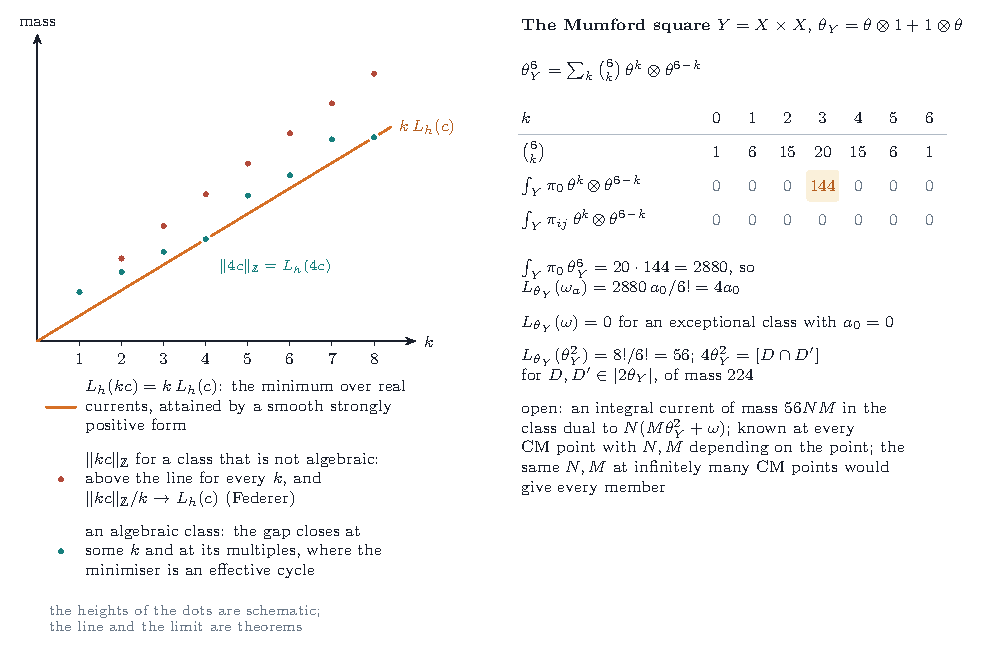
\includegraphics[width=\textwidth]{fig_massgap}
\caption{\Cref{thm:massgap} and \Cref{ex:mumfordmass}. Left: the mass of a
current in the class dual to $kc$ against $k$. The line $k\,L_{h}(c)$ is the
minimum over closed real normal currents, attained by a smooth strongly
positive form; the minima over closed integral currents lie on or above it,
with $\|kc\|_{\ZZ}/k\to L_{h}(c)$ by Federer's theorem, and for $M$ large the
class is algebraic exactly when one of them lies on the line, where the minimiser is
an effective algebraic cycle. The heights of the dots are schematic. Right:
the numbers of the Mumford square, in the split model. Of the seven terms $\binom6k\theta^{k}\otimes\theta^{6-k}$ of
$\theta_{Y}^{6}$ only $k=3$ pairs with $\pi_{0}=\frac14\theta\otimes\theta$,
giving $20\cdot144=2880$, and none pairs with the primitive summands; so
$L_{\theta_{Y}}(\omega_{a})=4a_{0}$, the Wirtinger bound of an exceptional
class with $a_{0}=0$ is zero, and the perturbation of $NM\theta_{Y}^{2}$ by
$N\omega$ changes the bound $56NM$ by nothing.}
\label{fig:massgap}
\end{figure}

\subsection{The routes at a glance}

\begingroup
\renewcommand{\arraystretch}{1.25}
\begin{longtable}{@{}>{\raggedright\arraybackslash}p{0.30\linewidth}>{\raggedright\arraybackslash}p{0.30\linewidth}>{\raggedright\arraybackslash}p{0.30\linewidth}@{}}
\caption{The routes considered, and the boundary of each result.}
\label{tab:scope}\\
\toprule
\textbf{Route} & \textbf{Result} & \textbf{Beyond the result} \\
\midrule
\endfirsthead
\multicolumn{3}{@{}l}{\footnotesize\itshape Table \thetable, continued.}\\[2pt]
\toprule
\textbf{Route} & \textbf{Result} & \textbf{Beyond the result} \\
\midrule
\endhead
\midrule
\multicolumn{3}{r@{}}{\footnotesize\itshape continued on the next page}\\
\endfoot
\bottomrule
\endlastfoot
Ambient object, restricted to $\Av$, transported by $\Phi_{\cP}$
  & closed by \cite[Theorem~7.3]{paperI}
  & ambient varieties with exceptional classes \\
Any $K$-equivariant construction with the norm character
  & closed by \cite[Theorem~5.6]{paperI}
  & constructions that are not eigenclasses \\
Secant dimension count
  & no obstruction, \cite[Corollary~8.4]{paperI}
  & none \\
Semiregularity dimension count
  & no obstruction, \cite[Corollary~9.3]{paperI}
  & none \\
Semiregularity of an object whose Chern character sits on the Weil line
  & closed by \cite[Theorem~9.7]{paperI} and \cite[Corollary~9.18]{paperI} for direct
    sums, and for every object by \cite[Theorem~3.5]{paperII}, for every CM field by
    \cite[Theorem~5.4]{paperII}
  & objects of positive rank; the weaker hypothesis of
    \cite[Question 11.4]{Mar25b} \\
The polarised criterion at a quartic CM field, $n=2$
  & computed for every shape, \cite[Theorem~5.14]{paperII}: a complex meeting it
    has $\dim\Ext^{2}(E,E)\ge88$, \cite[Corollary~5.15]{paperII}
  & existence of such a complex \\
Induction through hyperplane sections
  & closed by \cite[Theorem~10.3]{paperI}, \cite[Theorem~10.8]{paperI}
  & correspondences, degenerations, coniveau \\
Kuga--Satake, from a weight two structure of K3 type
  & not obstructed, \cite[Proposition~11.9]{paperI}
  & available only at $n=1$, \cite[Corollary~11.12]{paperI} \\
Divisors, on a member with quaternionic multiplication
  & succeeds, \cite[Theorem~15.25]{paperI}
  & fails at full Hodge group, \cite[Proposition~15.18]{paperI} \\
Propagation off the base locus
  & reduced to one bound or one rank, \cite[Theorem~16.9]{paperI},
    \cite[Theorem~2.3]{paperII}
  & the bound or the rank, \cite[Remark~3.7]{paperII} \\
Objects with effective Chern character at a base point
  & closed by \cite[Theorem~4.5]{paperII}
  & objects indecomposable in $D^{b}$, \cite[Remark~4.8]{paperII} \\
The weakened criterion for a secant object of positive rank
  & reduced to two conditions on the factor, \cite[Theorem~4.56]{paperII}, the first
    automatic for Markman's construction, \cite[Corollary~4.57]{paperII}; the
    identity fails for Markman's candidate, \cite[Theorem~4.61]{paperII}, and at every
    transversal double point, \cite[Corollary~4.63]{paperII}
  & objects whose support has no such point, \cite[Remark~4.64]{paperII} \\
A secant object $\cI_{S}(b\Theta)$ with smooth support
  & invariants forced and $d\le b^{2}$, so $d\le9$ at $b=3$,
    \cite[Theorem~4.67]{paperII}, \cite[Corollary~4.68]{paperII}
  & existence for $d\in\{1,3,5,7\}$ at $b=3$, one vanishing in
    $H^{1}(S,N_{S/X})$ and first-order extension, \cite[Remark~4.69]{paperII} \\
The local part of the weakened criterion
  & it is a condition on depth: no obstruction at a Cohen--Macaulay point,
    \cite[Theorem~4.75]{paperII}, \cite[Corollary~4.77]{paperII}
  & Cohen--Macaulay supports, where the identity becomes one global
    vanishing beside first-order extension \\
A support that is a complete intersection
  & closed for every $b$ and every $d$, \cite[Theorem~4.81]{paperII}
  & supports of higher Hilbert--Burch rank, \cite[Proposition~4.86]{paperII} \\
A support with a Hilbert--Burch resolution by line bundles or by simple
semi-homogeneous bundles
  & closed for every rank, twist and $d$, \cite[Theorem~4.89]{paperII},
    \cite[Theorem~4.92]{paperII}
  & resolutions over bundles that are not projectively flat \\
The secant route, granted every demand it makes
  & reaches $\delta=\delta_{0}$, and every $\delta$ by \Cref{prop:descent},
    \Cref{thm:closure}(iv)
  & the CM fields of degree at least four, which give the quadratic ones by
    \Cref{prop:descent}(ii) \\
Propagation from a base point
  & closes every imaginary quadratic family at once, \cite[Theorem~16.9]{paperI},
    \cite[Theorem~2.3]{paperII}
  & (P2) for the family, \Cref{cor:fourremain} \\
The bounded form (P1), read on the transported cycle
  & closed: the transport spreads each component by $c^{2n}/m_{i}$ and the
    data is unbounded whenever a component has finite stabiliser,
    \cite[Lemma~16.14]{paperI}, \cite[Theorem~16.15]{paperI}
  & nothing; the other reading is closed too \\
The bounded form (P1), read on the minimal representative
  & closed: equivalent to the conjecture for the family,
    \cite[Theorem~16.17]{paperI}
  & nothing; it is a restatement, so it is not a route \\
The pure form of (P2), for a given representative
  & forces the evaluation map to vanish on the $4n^{2}$-dimensional
    annihilator, and excludes every representative that is a sheaf on a
    smooth germ of codimension two of its support, \cite[Theorem~2.5]{paperII},
    \cite[Corollary~2.6]{paperII}
  & nothing: no representative exists, \cite[Theorem~3.5]{paperII} \\
The same form, tested by a number
  & $\dim\Ext^{2}(E,E)=2n(2n-1)$ at one base point would suffice,
    \cite[Theorem~2.11]{paperII}, and no representative attains it,
    \cite[Theorem~3.5]{paperII}
  & nothing \\
The same form, for a representative in codimension $n$
  & closed at every member of every family: the support must have a
    component of codimension less than $n$, and at a general member every
    component of codimension at least two has multiplicity zero,
    \cite[Lemma~2.12]{paperII}, \cite[Theorem~2.13]{paperII}
  & nothing: no representative exists, \cite[Theorem~3.5]{paperII} \\
The Hochschild action on such a representative
  & the annihilator is the mixed part of a splitting of $HH^{1}$ and the
    action factors through a ring of dimension $2^{2n+1}-1$ in one of
    dimension $2^{4n}$, \cite[Theorem~2.8]{paperII}, \cite[Corollary~2.9]{paperII}
  & nothing: no such complex exists, \cite[Theorem~3.5]{paperII} \\
The shape of such a representative
  & an indecomposable summand carries the class; at $n=2$, and at $n=3$
    granting the compatibility of \cite[Corollary~2.9(iii)]{paperII}, its
    endomorphism algebra has dimension at least three, so no simple object
    serves, \cite[Theorem~2.14]{paperII}
  & nothing: no object of any shape meets the pure form, \cite[Theorem~3.5]{paperII} \\
The pure form of (P2), Chern character exactly a Weil class
  & false for every imaginary quadratic field and every $n\ge2$: a
    semiregular such complex would deform to very general non-algebraic Weil
    tori, whose coherent sheaves have no Chern character below the top
    degree, \cite[Proposition~3.4]{paperII}, \cite[Theorem~3.5]{paperII}
  & the polarised form (P2$'$), whose Chern character may carry powers of
    the polarisation, \cite[Remark~3.6]{paperII} \\
The reduction to Weil classes, and to abelian varieties
  & false as a statement about Hodge rings in dimension eight,
    \Cref{prop:mumfordproduct}; impossible Hodge-theoretically,
    \Cref{prop:noabeliantype}
  & the algebraicity of the classes beyond the Weil lines, which is (F2), and
    (F3), which is the whole conjecture, \Cref{prop:f3ishc} \\
The two classes on the self-product of a Mumford fourfold
  & a real multiplication by a cubic field on the primitive part of $H^{2}$,
    algebraic once the Kuga--Satake class of one K3 surface of Picard number
    thirteen is, \Cref{prop:mumfordrm}, \Cref{thm:mumfordks}
  & that Kuga--Satake class, \Cref{rem:mumfordks} \\
Other routes to the same two classes
  & degeneration and larger families closed off by rigidity; semiregularity
    reduced to $\dim\Ext^{2}=119$ at one CM point; specialisation reduced to
    a degree bound, \Cref{thm:mumfordrigid}, \Cref{thm:mumfordnumerical},
    \Cref{cor:mumfordbounded}
  & an object with $\dim\Ext^{2}=119$, or the degree bound,
    \Cref{rem:bypassaudit} \\
The cycles at a CM point, for the same two classes
  & the fourfold is of Weil type for $k_{c}\subset\End^{0}(X_{c})$ with the
    two exotic classes as its Weil line; pull-backs of that line along
    homomorphisms with components in $k_{c}$ span, with divisor products,
    $110$ of the $132$ Hodge classes of the square and no exceptional class,
    and an exceptional class is reached exactly by components generating the
    endomorphism algebra over $k_{c}$, \Cref{prop:cmsource}
  & a degree bound for cycles using the real multiplication, at infinitely
    many CM points, \Cref{rem:cmsource} \\
Objects built from line bundles, for the same two classes
  & closed at every point of the curve: the Chern characters stay invariant
    under the Lefschetz group, \Cref{thm:lefschetzclosure}
  & steps that break that symmetry, \Cref{rem:leavel} \\
Twistor deformation of the square, for the same two classes
  & closed: the component of the Hodge locus among all complex tori is the
    Mumford curve, which contains no twistor line, \Cref{prop:notwistor}
  & the Kuga--Satake class, which moves in a seven-dimensional family \\
Five further routes, for the same two classes
  & one statement: three of them are equivalent to the target and two imply
    it, so any one of them suffices, \Cref{cor:mumfordone}
  & the target itself, which is only the first case of (F2),
    \Cref{rem:mumfordneeded} \\
Pull-back from a hyperk\"ahler manifold, for the same two classes
  & the square is holomorphic symplectic and the classes are the twisted dual
    forms of the part of $H^{2}$ its symplectic class generates; a symplectic
    rational map to some $S_{\mu}^{[n]}$, $n\ge5$, suffices, and no K3
    surface or hyperk\"ahler eightfold serves, \Cref{prop:hksquare}
  & such a map, \Cref{rem:hkroute} \\
Reduction modulo $p$, for the same two classes
  & represented by cycles at every closed point of every reduction; the
    target is equivalent to a bound on their Hilbert data on a Zariski dense
    set, \Cref{prop:modp}, \Cref{thm:modpdensity}
  & the bound, \Cref{rem:modpremains} \\
The Weil classes of every CM field
  & the same propagation problem, with a CM base point in every family,
    \cite[Theorem~17.5]{paperI}, \cite[Theorem~17.7]{paperI}
  & (P2) for the split families \\
Routes from outside algebraic geometry
  & positivity of currents sees nothing; the conjecture is the vanishing of
    the integrality gap of a mass minimisation whose real version is solved,
    \Cref{prop:positivitynotest}, \Cref{thm:massgap}
  & a calibrated integral current in one class, \Cref{ex:mumfordmass} \\
The closure, as a whole
  & five minimal sets of hypotheses: $\{\mathrm{F3}\}$ and
    $\{\mathrm{L},\mathrm{M}\}$, each equivalent to the conjecture, and
    three through the conjecture modulo abelian varieties,
    $\{\mathrm{L},\mathrm{F3}'\}$, $\{\mathrm{V},\mathrm{F3}'\}$ and this
    route, $\{\mathrm{P2}_{\mathrm{split}},\mathrm{F2},\mathrm{F3}'\}$,
    \Cref{thm:closure}, \Cref{prop:f3ishc}, \Cref{cor:fourremain},
    \Cref{rem:bullseye}
  & the Lefschetz standard conjecture, (M), (V), (F2), (F3$'$) \\
Convolutions of the Weil pieces on $E_{0}^{2n}$
  & at $n=3$ every convolution has $\dim\Ext^{2}\ge69>57$,
    \cite[Theorem~4.35]{paperII}; at $n=4$, with the pieces at two shifts,
    $\dim\Ext^{2}\ge40960>104$, \cite[Theorem~4.37]{paperII}, at three
    consecutive shifts $\dim\Ext^{2}\ge22528$, \cite[Theorem~4.38]{paperII},
    with the shifts within six consecutive values $\dim\Ext^{2}\ge640$,
    \cite[Corollary~4.48]{paperII}, and with each parity at one shift, at any odd
    distance, $\dim\Ext^{2}\ge1792$, \cite[Proposition~4.46]{paperII}
  & the other arrangements of the shifts at $n=4$,
    \cite[Remark~4.50]{paperII} \\
Diagonal complete intersections of Vandermonde type
  & quotients of powers of a generalised Fermat curve, so in $\mathcal{A}$;
    the conjecture holds when it holds on the abelian varieties $B_{[a]}$, and
    holds for two diagonal hypersurfaces of degree $3$, $4$, $6$ in
    $\PP^{6}$, \Cref{thm:vandermonde}, \Cref{cor:twodiagonal}; it holds on
    the very general member for $d=2$ in every dimension, for $d=3,4$ up
    to dimension seven and for $d=6$ up to dimension five,
    \Cref{thm:vgvandermonde}
  & $B_{[a]}$ of dimension above five, the Weil classes of
    $\QQ(\zeta_{e})$ with $\varphi(e)\ge4$, and the very general member
    for $d=3,4,6$ from dimension eight on and for $d=6$ in dimension six,
    \Cref{rem:vandermonde} \\
The conjecture modulo abelian varieties, (F3$'$)
  & holds on the class $\mathcal{A}$ of varieties whose cohomology is
    reached from abelian varieties by algebraic correspondences (curves,
    abelian varieties, products, surjective images), in degrees $0$, $2$,
    $2n-2$, $2n$, and in dimension at most three, \Cref{prop:f3prime};
    on the Delsarte hypersurfaces and the diagonal complete intersections
    of Vandermonde type, \Cref{cor:delsarteall}, \Cref{thm:vandermonde};
    on the fourfolds and fivefolds of \Cref{prop:f3primesmall},
    \Cref{prop:f3primefibration} and \Cref{prop:f3primedominant};
    through the Hodge conjecture on the varieties of \Cref{prop:k3powers}
    and \Cref{prop:k3ntype}
  & degree four on fourfolds outside $\mathcal{A}$ not covered by these
    results, and beyond, for
    instance squares of K3 surfaces with real multiplication, such as
    $S_{\lambda}$, \Cref{rem:f3primeopen},
    \Cref{rem:f3primefrontier} \\
\end{longtable}
\endgroup

\section{Hodge classes beyond the Weil lines}\label{sec:beyond}

\subsection{The first classes beyond the Weil lines}\label{ssec:mumford}

Statement (F2) is the Hodge conjecture for the Hodge classes on abelian
varieties that no Weil line reaches, and \Cref{prop:mumfordproduct} exhibits
the first of them: two classes in $H^{4}(X\times X,\QQ)$ for an abelian
fourfold $X$ of Mumford type. None of the constructions of the preceding
sections acts on them. In this subsection we identify them as a real
multiplication on the primitive part of $H^{2}(X)$, and we prove that they
are algebraic as soon as the Kuga--Satake class of one K3 surface of Picard
number thirteen attached to $X$ is algebraic. We do not prove that the
Kuga--Satake class is algebraic, and we know of no proof. The reduction
changes the kind of question: two classes on an eightfold are traded for one
correspondence of a well-studied type, between a surface and its Kuga--Satake
variety. The cubic field of the real multiplication enters through the
Clifford relations, which force the blocks of the Kuga--Satake embedding to
span it.

\begin{setupenv}[Mumford type]\label{setup:mumford}
Let $X$ be as in \Cref{prop:mumfordproduct}, with $V=H^{1}(X,\QQ)$,
polarisation $\psi$ and polarisation class $\theta\in H^{2}(X,\QQ)$, and let
$G=\Hg(X)$. Over $\bar{\QQ}$ the Hodge cocharacter is nontrivial on exactly
one of the three factors of $G$: on $V_{i}$ it has weights $\pm a_{i}/2$ with
$a_{i}\ge0$, and $V$ has only the two weights $\pm\frac12$, so exactly one
$a_{i}$ is nonzero. Since $\End^{0}(X)=\QQ$, it follows that $G$ is
$\QQ$-simple: the Lie algebra of a $\QQ$-factor not containing that geometric
factor would consist of Hodge classes in $\End(V)$, that is, of endomorphisms
of $X$. So $G$ is the image in
$\GL(V)$ of $\Res_{F/\QQ}D^{1}$, where $F$ is a totally real cubic field, $D$
is a quaternion algebra over $F$ split at one real place $\sigma_{3}$ and
definite at the other two, $\sigma_{1}$ and $\sigma_{2}$, with
$\operatorname{Cor}_{F/\QQ}D\cong M_{8}(\QQ)$, and $D^{1}$ is the group of
elements of reduced norm one \cite{Mum69,Gal00}; the kernel is the central
subgroup of triples of signs with product one. Over $\bar{\QQ}$,
$V=V_{1}\otimes V_{2}\otimes V_{3}$, where $V_{i}$ is the standard
representation of $D\otimes_{F,\sigma_{i}}\bar{\QQ}=M_{2}(\bar{\QQ})$; the
Galois group permutes the three factors as it permutes the three embeddings,
and $H^{1,0}(X)=V_{1}\otimes V_{2}\otimes V_{3}^{1,0}$. Put
\[
  T=\operatorname{Lie}G=D^{0},
  \qquad
  q_{\lambda}(x,y)=\Tr_{F/\QQ}\bigl(\lambda\operatorname{trd}(xy)\bigr)
  \quad(\lambda\in F^{\times}),
\]
where $D^{0}$ is the space of quaternions of reduced trace zero, regarded as
a $\QQ$-vector space of dimension nine, and $\operatorname{trd}$ is the
reduced trace. Over $\bar{\QQ}$, $T=T_{1}\oplus T_{2}\oplus T_{3}$ with
$T_{i}=\mathfrak{sl}(V_{i})$, and $a\in F$ acts on $T_{i}$ by $\sigma_{i}(a)$.
Write $m_{a}$ for multiplication by $a$. The space $T\subset\End(V)$ is a
sub-Hodge structure of weight zero.
\end{setupenv}

\begin{proposition}[The two classes are a real multiplication]%
\label{prop:mumfordrm}
In \Cref{setup:mumford}:
\begin{enumerate}[label=\textup{(\roman*)},nosep,leftmargin=2.6em]
\item $H^{2}(X,\QQ)=\QQ\theta\oplus U$, where $U$ is the primitive part, of
  dimension $27$, and over $\bar{\QQ}$
  \[
    U=U_{12}\oplus U_{13}\oplus U_{23},\qquad
    U_{ij}=S^{2}V_{i}\otimes S^{2}V_{j}\otimes{\textstyle\bigwedge^{2}}V_{k},
    \quad \{i,j,k\}=\{1,2,3\},
  \]
  each of dimension nine. The summand $U_{12}$ is of type $(1,1)$, and
  $U_{13}$ and $U_{23}$ have Hodge numbers $(3,3,3)$.
\item The algebra of Hodge endomorphisms of $H^{2}(X,\QQ)$ is $\QQ\times F$,
  acting by scalars on $\QQ\theta$, with $a\in F$ acting on $U_{ij}$ by
  $\sigma_{k}(a)$. Through Poincar\'e duality and the Lefschetz isomorphism
  $\theta^{2}\colon H^{2}\to H^{6}$ this algebra is the space of Hodge classes
  in the K\"unneth component $H^{2}(X)\otimes H^{2}(X)$ of
  $H^{4}(X\times X,\QQ)$; the subalgebra $\QQ\times\QQ$ is spanned by the
  products of divisor classes that lie there, and the two classes of
  \Cref{prop:mumfordproduct}(ii) may be taken to be the elements of $F$ of
  trace zero.
\item $T(-1)$ is a Hodge structure of K3 type with Hodge numbers $(1,7,1)$,
  and its Hodge endomorphisms are the $m_{a}$, $a\in F$. The $G$-invariant
  symmetric forms on $T$ are the $q_{\lambda}$, and $q_{\lambda}$ polarises
  $T(-1)$ if and only if $\lambda$ is totally positive.
\end{enumerate}
\end{proposition}

\begin{proof}
(i) is the decomposition of $\bigwedge^{2}(V_{1}\otimes V_{2}\otimes V_{3})$
in the proof of \Cref{prop:mumfordproduct}, where $U_{ij}$ appears as the
summand of highest weight $2$ on the $i$-th and $j$-th factors. The Hodge
cocharacter acts trivially on $V_{1}$ and $V_{2}$ and splits
$V_{3}=V_{3}^{1,0}\oplus V_{3}^{0,1}$, so $\bigwedge^{2}V_{3}$ has type
$(1,1)$ and $S^{2}V_{3}$ has one dimension of each of the types $(2,0)$,
$(1,1)$, $(0,2)$.

(ii) A Hodge endomorphism commutes with the Mumford--Tate group
$G\cdot\mathbb{G}_{m}$, and $\mathbb{G}_{m}$ acts on $H^{2}$ by scalars, so
the Hodge endomorphisms are the $G$-endomorphisms. Over $\bar{\QQ}$ the four
summands $\QQ\theta$, $U_{12}$, $U_{13}$, $U_{23}$ are irreducible and
pairwise non-isomorphic, so the $G$-endomorphisms are the combinations of the
four projections. The Galois group fixes the projection onto $\QQ\theta$ and
permutes the other three as it permutes the indices $k$, that is, as it
permutes the embeddings of $F$. For $a\in F$ an endomorphism acting on
$U_{ij}$ by $\sigma_{k}(a)$ is therefore Galois invariant, hence rational, and
with the scalars on $\QQ\theta$ these exhaust the rational points, which form
$\QQ\times F$. Poincar\'e duality identifies $\End H^{2}(X,\QQ)$ with
$H^{6}(X)\otimes H^{2}(X)$, and $\theta^{2}\otimes1$ carries
$H^{2}\otimes H^{2}$ onto it; both are given by algebraic classes, and on an
abelian variety so is the inverse of the Lefschetz isomorphism
\cite[\S2]{Kle68}. The products of divisor classes in $H^{2}\otimes H^{2}$
are $\psi_{11}\psi_{22}$ and $\psi_{12}^{2}$ in the notation of the proof of
\Cref{prop:mumfordproduct}. They are invariant under the whole of
$\Sp(V,\psi)$, whose endomorphisms of $H^{2}=\QQ\theta\oplus U$ are spanned
by the identity and the projection onto $\QQ\theta$, and they are linearly
independent, being a multiple of the projection and a multiple of the
identity (proof of \Cref{prop:mumfordproduct}); so they span $\QQ\times\QQ$, and any complement of
$\QQ\times\QQ$ in $\QQ\times F$ may serve as the two remaining classes.

(iii) The adjoint action of the Hodge cocharacter is trivial on $T_{1}$ and
$T_{2}$ and has weights $-1$, $0$, $1$ on $T_{3}$, so $T$ has Hodge numbers
$(1,7,1)$ in the types $(-1,1)$, $(0,0)$, $(1,-1)$, and $T(-1)$ is of K3
type. Its Hodge endomorphisms are again the $G$-endomorphisms, and the
argument of (ii), applied to the three pairwise non-isomorphic summands
$T_{i}$, gives $F$ acting by multiplication. On each $T_{i}$ the invariant
symmetric forms are the multiples of $\operatorname{tr}(xy)$, and
$\operatorname{tr}(x_{i}y_{i})=\sigma_{i}(\operatorname{trd}(xy))$ for
$x,y\in D^{0}$, so the Galois-invariant ones are the $q_{\lambda}$. At
$\sigma_{1}$ and $\sigma_{2}$ the algebra $D\otimes\RR$ is Hamilton's
quaternions, $T_{i}$ is of type $(1,1)$, and
$\operatorname{trd}(x^{2})=-2\operatorname{nrd}(x)$ is negative on nonzero
pure quaternions. At $\sigma_{3}$ the form
$\operatorname{tr}(xy)$ on $\mathfrak{sl}_{2}(\RR)$ is negative on the line of
type $(1,1)$, the Lie algebra of the rotations fixed by the Hodge
cocharacter, and positive on its orthogonal complement, the real points of
the types $(2,0)$ and $(0,2)$. The Hodge--Riemann relations for a structure
of K3 type ask for exactly these signs after multiplication by
$\sigma_{i}(\lambda)$, so $q_{\lambda}$ polarises $T(-1)$ precisely when every
$\sigma_{i}(\lambda)$ is positive.
\end{proof}

The two classes are thus the endomorphisms of $U$ given by the elements of
$F$ of trace zero. A Hodge structure of K3 type with the same field sits
beside them, and the next lemma connects the two.

\begin{lemma}[The product map]\label{lem:mumfordmu}
For $x,y\in T$ let $\mu(x\otimes y)\in H^{2}(X,\QQ)$ be the class that
corresponds under $\psi$ to the alternating form
$(v,w)\mapsto\psi(xv,yw)+\psi(yv,xw)$ on $V$. Then $\mu$ is a $G$-equivariant
map $T\otimes T\to H^{2}(X,\QQ)$, and:
\begin{enumerate}[label=\textup{(\roman*)},nosep,leftmargin=2.6em]
\item for $i\ne j$ it restricts to an isomorphism $T_{i}\otimes T_{j}\to
  U_{ij}$, and it carries $T_{i}\otimes T_{i}$ onto $\QQ\theta$;
\item for $e,\lambda\in F^{\times}$ put $\mu_{e}=\mu\circ(m_{e}\otimes m_{e})$
  and let $\mu_{e}^{\dagger}$ be its adjoint for the form
  $q_{\lambda}\otimes q_{\lambda}$ on $T\otimes T$ and the Lefschetz pairing
  $B(\alpha,\beta)=\int_{X}\alpha\beta\,\theta^{2}$ on $H^{2}(X,\QQ)$. Then
  $\mu_{e}\mu_{e}^{\dagger}$ preserves $\QQ\theta$ and acts on $U$ as the
  element
  \[
    \nu\,\Nm_{F/\QQ}(g)\,g^{-1}\in F,\qquad g=e^{2}/\lambda,
  \]
  where $\nu$ is a nonzero rational number independent of $e$ and $\lambda$.
\end{enumerate}
\end{lemma}

\begin{proof}
Equivariance is clear, since $\mu$ is built from $\psi$ and the action of
$\End(V)$ on $V$. An element $x\in T_{i}$ acts on $V$ through the $i$-th factor
and lies in the symplectic Lie algebra of $\psi=\epsilon_{1}\otimes
\epsilon_{2}\otimes\epsilon_{3}$, so $\psi(xv,yw)=-\psi(v,xyw)$ and
$\mu(x\otimes y)$ is the form $-\psi(v,(xy+yx)w)$. If $x\in T_{i}$ and
$y\in T_{j}$ with $i\ne j$, then $xy=yx$ acts as $x\otimes y$ on
$V_{i}\otimes V_{j}$, and the form is $-2$ times the product of
$\epsilon_{i}(\cdot,x\,\cdot)$, $\epsilon_{j}(\cdot,y\,\cdot)$ and
$\epsilon_{k}$; the first two are symmetric because $x$ and $y$ lie in
$\mathfrak{sp}(\epsilon)=\mathfrak{sl}_{2}$, and $x\mapsto\epsilon(\cdot,x\,\cdot)$
is an isomorphism $\mathfrak{sl}_{2}\to S^{2}V^{\vee}$, so $\mu$ maps
$T_{i}\otimes T_{j}$ isomorphically onto $U_{ij}$. If $i=j$, then
$xy+yx=\operatorname{tr}(xy)$ on $V_{i}$, because $x$ and $y$ are trace-free
$2\times2$ matrices, and $\mu(x\otimes y)=-\operatorname{tr}(xy)\,\theta$.

For (ii), $m_{e}$ is self-adjoint for $q_{\lambda}$, and the adjoint of a
map out of $(T\otimes T,q_{\lambda}\otimes q_{\lambda})$ is
$(m_{\lambda}\otimes m_{\lambda})^{-1}$ times its adjoint for
$q_{1}\otimes q_{1}$, so
$\mu_{e}\mu_{e}^{\dagger}=\mu\,(m_{g}\otimes m_{g})\,\mu^{\dagger_{1}}$ with
$\mu^{\dagger_{1}}$ the adjoint for $q_{1}\otimes q_{1}$. This map is
$G$-equivariant, so it preserves $\QQ\theta$ and each $U_{ij}$, and
$\mu^{\dagger_{1}}$ carries $U_{ij}$ into
$(T_{i}\otimes T_{j})\oplus(T_{j}\otimes T_{i})$, on which $m_{g}\otimes m_{g}$
is multiplication by $\sigma_{i}(g)\sigma_{j}(g)=\Nm(g)/\sigma_{k}(g)$. Hence
$\mu_{e}\mu_{e}^{\dagger}$ is $\Nm(g)\sigma_{k}(g)^{-1}$ times
$\mu\mu^{\dagger_{1}}$ on $U_{ij}$. The summands of $H^{2}(X,\bar{\QQ})$ are
pairwise non-isomorphic and self-dual, so $B$ is nondegenerate on $U_{ij}$,
and by Schur's lemma the pull-back of $B$ along the isomorphism
$\mu_{0}=\mu|_{T_{i}\otimes T_{j}}$ is $c_{k}\,q_{1}\otimes q_{1}$ with
$c_{k}\ne0$; then $\mu_{0}\mu_{0}^{\dagger_{1}}=c_{k}$ on $U_{ij}$. As $\mu$
is symmetric in its two arguments and the exchange of the factors is an
isometry of $q_{1}\otimes q_{1}$, $\mu^{\dagger_{1}}u=\mu_{0}^{\dagger_{1}}u+
s\,\mu_{0}^{\dagger_{1}}u$ with $s$ that exchange, and $\mu\mu^{\dagger_{1}}=2c_{k}$
on $U_{ij}$. On the split model $V=\bar{\QQ}^{2}\otimes\bar{\QQ}^{2}\otimes
\bar{\QQ}^{2}$, $\psi=\epsilon\otimes\epsilon\otimes\epsilon$, the
permutations of the three factors preserve $\psi$, hence $\theta$, $B$ and
$\mu$, and also $q_{1}=\sum_{i}\operatorname{tr}(x_{i}y_{i})$, while they
permute the $U_{ij}$; so $c_{1}=c_{2}=c_{3}$, and $\mu\mu^{\dagger_{1}}$ is one
and the same nonzero number $\nu$ on the three summands $U_{ij}$, rational
because $\mu\mu^{\dagger_{1}}$ is defined over $\QQ$. By \Cref{prop:mumfordrm}(ii) an endomorphism of $U$ acting
on $U_{ij}$ by $\nu\Nm(g)/\sigma_{k}(g)$ is the element $\nu\Nm(g)g^{-1}$ of
$F$.
\end{proof}

\Cref{fig:mumford} draws \Cref{prop:mumfordrm} and \Cref{lem:mumfordmu} over
the three factors of the Hodge group.

By the Kuga--Satake class of a projective K3 surface $S$ we mean the Hodge
class on $S\times\mathrm{KS}(S)\times\mathrm{KS}(S)$ that induces the embedding
of \cite[Proposition~11.7]{paperI} for $T(S)_{\QQ}$; its algebraicity is the Kuga--Satake
Hodge conjecture for $S$ (\cite[Remark~11.8]{paperI}).

\begin{theorem}[One K3 surface for the two classes]\label{thm:mumfordks}
In \Cref{setup:mumford}, let $\lambda\in F$ be totally positive.
\begin{enumerate}[label=\textup{(\roman*)},nosep,leftmargin=2.6em]
\item There is a projective K3 surface $S_{\lambda}$ of Picard number
  thirteen and an isomorphism of Hodge structures
  $T(S_{\lambda})_{\QQ}\cong T(-1)$ carrying the intersection form to
  $q_{\lambda}$. Its Kuga--Satake variety is isogenous to $X^{32}$.
\item If the Kuga--Satake class of $S_{\lambda}$ is algebraic, then the real
  multiplication by $F$ on $T(S_{\lambda})$ is induced by algebraic cycles on
  $S_{\lambda}\times S_{\lambda}$, and every Hodge class in
  $H^{4}(X\times X,\QQ)$ is algebraic; in particular the two classes of
  \Cref{prop:mumfordproduct}(ii) are algebraic.
\end{enumerate}
\end{theorem}

\begin{proof}
(i) The quadratic space $(T,q_{\lambda})$ has dimension nine and signature
$(2,7)$ by \Cref{prop:mumfordrm}(iii), and $H^{2}$ of a K3 surface with its
intersection form has dimension $22$ and signature $(3,19)$. Over $\QQ_{p}$
a nondegenerate quadratic space embeds isometrically in every nondegenerate
space of dimension at least three larger, and over $\RR$ the signatures
allow it, so by the Hasse--Minkowski theorem for representations of forms by
forms \cite[\S\S63, 66]{OMe00} there is an isometric embedding of
$(T,q_{\lambda})$ into $\Lambda_{\QQ}$, where $\Lambda$ is the K3 lattice.
The line $\ell=T(-1)^{2,0}\subset T_{\CC}\subset\Lambda_{\CC}$ satisfies
$(\ell,\ell)=0$ and $(\sigma,\bar{\sigma})>0$ for $0\ne\sigma\in\ell$, so by the
surjectivity of the period map there is a K3 surface $S_{\lambda}$ with a
marking $H^{2}(S_{\lambda},\ZZ)\cong\Lambda$ that carries
$H^{2,0}(S_{\lambda})$ to $\ell$ \cite[Chs.~6--7]{Huy16}. A rational class
is of type $(1,1)$ exactly when it is orthogonal to $\ell$, and its component
in $T$ is then a rational class of type $(1,1)$ in $T(-1)$, that is a
$G$-invariant vector of $T=\operatorname{Lie}G$; there is none, since $G$ is
semisimple. So $\NS(S_{\lambda})_{\QQ}=T^{\perp}$, of dimension $13$ and
signature $(1,12)$, and $T(S_{\lambda})_{\QQ}=T$ with the form $q_{\lambda}$.
A class of positive square in $\NS(S_{\lambda})$ makes $S_{\lambda}$
projective \cite[Ch.~8]{Huy16}.

For the Kuga--Satake variety, note first that over $\bar{\QQ}$ the space $T$
is the orthogonal sum of the three ternary spaces $T_{i}$, so $C(T)$ is the
graded tensor product of the $C(T_{i})$. Scaling a ternary form does not
change its even Clifford algebra, so $D^{1}$ is the spin group of
$(D^{0},\lambda\operatorname{trd})$ for every $\lambda$, and
$\Res_{F/\QQ}D^{1}$ maps to $\mathrm{Spin}(T,q_{\lambda})$ by multiplication
in the Clifford algebra, with the same kernel as its map to $\GL(V)$, so that
$G$ is a subgroup of $\mathrm{Spin}(T,q_{\lambda})$; as a representation of
the $i$-th factor, $C(T_{i})$ is four copies of $V_{i}$. Hence $C^{+}(T)$ is
$V^{\oplus32}$ as a representation of $G$ over $\bar{\QQ}$, and over $\QQ$ as
well, because $V$ is absolutely irreducible. The Hodge structures on
$C^{+}(T)=H^{1}(\mathrm{KS}(S_{\lambda}),\QQ)$ and on
$V^{\oplus32}=H^{1}(X^{32},\QQ)$ are both given by lifts of weight one of the
same homomorphism $\mathbb{S}\to\MT(T)_{\RR}$ through $G\cdot\mathbb{G}_{m}$,
and two such lifts coincide.\footnote{They differ by a homomorphism from the
anisotropic torus $\mathbb{S}/\mathbb{G}_{m}$ to the centre of
$G\cdot\mathbb{G}_{m}$, whose identity component is $\mathbb{G}_{m}$, and
such a homomorphism is trivial.} So
$H^{1}(\mathrm{KS}(S_{\lambda}),\QQ)\cong H^{1}(X^{32},\QQ)$ as Hodge
structures, and $\mathrm{KS}(S_{\lambda})$ is isogenous to $X^{32}$. For the
form used by Galluzzi this is her theorem \cite{Gal00}; van Geemen proves the
corresponding splitting for every K3 surface with real multiplication
\cite{vG08}.

(ii) Write $S=S_{\lambda}$ and $A=\mathrm{KS}(S)$, and let $Z_{S}$ be an
algebraic cycle on $S\times A\times A$ inducing the Kuga--Satake embedding
$T(S)\to\End H^{1}(A)$. Composing $Z_{S}$ with the graph of an isogeny
$A\to X^{32}$ and with the graphs of the inclusions and projections of the
factors of $X^{32}$ gives algebraic cycles on $S\times X\times X$ inducing the
$32^{2}$ block components of the embedding, which are morphisms of Hodge
structures $T(S)\to\End(V)$, up to a Tate twist; both lie in the tensor
category generated by $H^{1}(X)$, so the blocks are equivariant for
$\MT(X)=G\cdot\mathbb{G}_{m}$. Over $\bar{\QQ}$,
$\End(V)=S^{2}V\oplus\bigwedge^{2}V$, and $T_{i}\cong S^{2}V_{i}$ occurs once
in $S^{2}V$, as $S^{2}V_{i}\otimes\bigwedge^{2}V_{j}\otimes\bigwedge^{2}V_{k}$,
and not at all in $\bigwedge^{2}V$. So each block takes values in $T$, and
through the identification of (i) it is a $G$-endomorphism of $T$, that is
$m_{e_{ab}}$ for some $e_{ab}\in F$ by \Cref{prop:mumfordrm}(iii). Over
$\bar{\QQ}$ the embedding is therefore $v\mapsto v\otimes N_{i}$ on $T_{i}$,
acting on $H^{1}(A)=V\otimes\QQ^{32}$, with
$N_{i}=(\sigma_{i}(e_{ab}))_{a,b}$. The embedding $\Psi$ of
\cite[Proposition~11.7]{paperI} satisfies the Clifford relation
$\Psi(v)\Psi(w)+\Psi(w)\Psi(v)=2q_{\lambda}(v_{0},v_{0})\,q_{\lambda}(v,w)$,
because
$\Psi(v)\Psi(w)x=vwx\,v_{0}^{2}$. Take nonzero $v\in T_{i}$ and
$w\in T_{j}$ with $i\ne j$. As endomorphisms of $V$ they commute and $vw\ne0$,
so the left side is $vw\otimes(N_{i}N_{j}+N_{j}N_{i})$, while the right side
is zero because $T_{i}$ and $T_{j}$ are orthogonal; hence $N_{i}$ and $N_{j}$
anticommute. For $v\in T_{i}$ with $q_{\lambda}(v,v)\ne0$ the relation reads
$v^{2}\otimes N_{i}^{2}=q_{\lambda}(v_{0},v_{0})\,q_{\lambda}(v,v)$, and $v^{2}$
is a nonzero scalar on $V_{i}$, so $N_{i}^{2}$ is a nonzero scalar. Three pairwise
anticommuting invertible matrices are linearly independent: multiplying a
relation $\sum_{i}c_{i}N_{i}=0$ by $N_{j}$ on either side and adding gives
$2c_{j}N_{j}^{2}=0$. If the $e_{ab}$ spanned a subspace of $F$ of dimension at
most two, the three $N_{i}$ would lie in the span of at most two rational
matrices, which is impossible; so the $e_{ab}$ span $F$, and two of them, $e$
and $e'$, are not rational multiples of each other. Then $(e/e')^{2}$ is irrational, since a cubic field
contains no irrational element with rational square, so $e^{2}/\lambda$ and
$e'^{2}/\lambda$ are not both rational. Fix a block $\kappa=m_{e}$ with
$e^{2}/\lambda\notin\QQ$, induced by a cycle $\Gamma$.

Consider first the real multiplication. The trace form
$(a,b)\mapsto\operatorname{tr}(ab)$ on $\End(V)$ is induced by an algebraic
class: for correspondences $a,b$ on $X$
the Lefschetz trace formula gives
$\operatorname{tr}(a_{*}b_{*}\mid H^{1})=-\deg\bigl((a\circ b\circ\pi_{1})\cdot\Delta_{X}\bigr)$,
where $\pi_{1}$ is the K\"unneth projector onto $H^{1}$, algebraic on an
abelian variety \cite[\S2]{Kle68}. So the adjoint $\kappa^{\dagger}$ of
$\kappa$, for this form and the intersection form on $S$, is induced by a
cycle built from the transpose of $\Gamma$, $\pi_{1}$ and $\Delta_{X}$, and
$\kappa^{\dagger}\kappa$ is an algebraic endomorphism of $T(S)$. An element
$x$ of $T_{i}$ acts on the eight-dimensional space $V$ through a
two-dimensional factor, with multiplicity four, so
$\operatorname{tr}_{V}(xy)=4\Tr_{F/\QQ}\operatorname{trd}(xy)$, and
\[
  q_{\lambda}(\kappa^{\dagger}\kappa x,y)
  =\operatorname{tr}_{V}(ex\cdot ey)
  =4\Tr_{F/\QQ}\bigl(e^{2}\operatorname{trd}(xy)\bigr)
  =q_{\lambda}\bigl(4e^{2}\lambda^{-1}x,y\bigr),
\]
that is $\kappa^{\dagger}\kappa=m_{4e^{2}/\lambda}$. By the choice of $e$ this
element is irrational, so it generates the cubic field $F$ and every $m_{a}$
is a polynomial in $\kappa^{\dagger}\kappa$. Composing with the projector of
$H^{2}(S)$ onto $T(S)$, which is algebraic because it is the diagonal minus
$[\mathrm{pt}\times S]$, $[S\times\mathrm{pt}]$ and $\sum_{r}d_{r}\times d_{r}^{\vee}$
over dual bases of $\NS(S)_{\QQ}$, gives algebraic cycles on $S\times S$
inducing the real multiplication.

Consider next the classes on $X\times X$. The map
$\mu_{\kappa}=\mu\circ(\kappa\otimes\kappa)$ from $T(S)\otimes T(S)$ to
$H^{2}(X,\QQ)$ is induced by an algebraic cycle on $S\times S\times X$,
obtained from $\Gamma\times\Gamma$, the divisor
$m^{*}\theta-p_{1}^{*}\theta-p_{2}^{*}\theta$ on $X\times X$, whose class is
$\psi$ in $H^{1}\otimes H^{1}$, and the diagonal of $X$ by pull-back,
push-forward and intersection, because $\mu$ uses nothing but $\psi$ and the
composition of endomorphisms of $V$. The form $q_{\lambda}\otimes q_{\lambda}$ is the intersection form of
$S\times S$ on $T(S)\otimes T(S)$ and $B$ is the intersection form of $X$
twisted by $\theta^{2}$, so the adjoint $\mu_{\kappa}^{\dagger}$ is induced by
cup product with $\theta^{2}$ followed by the transposed cycle, and
$E=\mu_{\kappa}\mu_{\kappa}^{\dagger}$ is an algebraic endomorphism of
$H^{2}(X,\QQ)$. Since $\kappa=m_{e}$, \Cref{lem:mumfordmu}(ii) says that $E$
preserves $\QQ\theta$ and acts on $U$ as $\nu\Nm(g)g^{-1}$ with
$g=e^{2}/\lambda$, and this element of $F$ is not rational, since $g$ is
not. The projection $\pi_{\theta}$ onto $\QQ\theta$ is algebraic, being
given by the class $\theta\times\theta$ suitably normalised, so the algebraic
Hodge endomorphisms of $H^{2}(X,\QQ)$ contain $1$, $\pi_{\theta}$ and
$E(1-\pi_{\theta})$, which generate $\QQ\times F$, that is all of them by
\Cref{prop:mumfordrm}(ii). By the same part every Hodge class in
$H^{2}(X)\otimes H^{2}(X)$ is then algebraic. The Hodge classes of
$H^{4}(X\times X,\QQ)$ in the other K\"unneth components number one in each
of $H^{a}\otimes H^{4-a}$, $a\ne2$, by the count in the proof of
\Cref{prop:mumfordproduct}, and are products of divisor classes.
\end{proof}

\begin{figure}[tbp]
\centering
  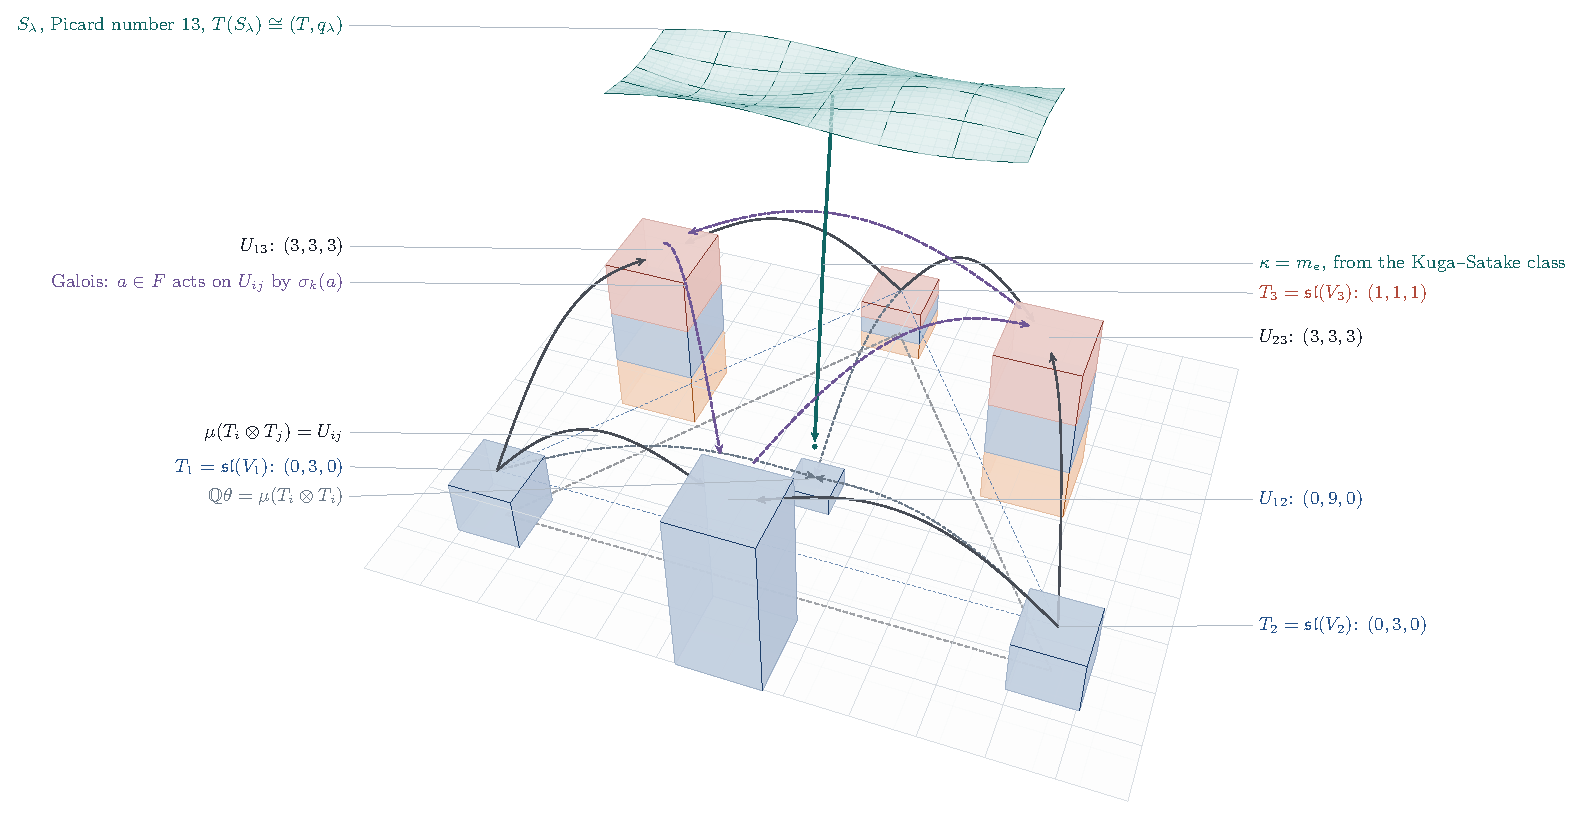
\includegraphics[width=\textwidth]{fig_mumford}
\caption{\Cref{prop:mumfordrm} and \Cref{lem:mumfordmu}, drawn over the
triangle of the three factors of the Hodge group; every height is a
dimension. At the corners stand the summands $T_{i}=\mathfrak{sl}(V_{i})$ of
$T=\operatorname{Lie}G$, banded by Hodge type after the Tate twist $T(-1)$: blue for
$(1,1)$, clay for $(2,0)$ and amber for $(0,2)$, so that only $T_{3}$ carries
the K3 type. On the edges stand the three summands $U_{ij}$ of the primitive
part of $H^{2}(X)$, of dimension nine, $U_{12}$ of pure type $(1,1)$ and the
other two in three bands of three; in the middle is the line of $\theta$. The
solid arcs are the product map $\mu$, which carries $T_{i}\otimes T_{j}$ onto
$U_{ij}$, and the dashed ones carry $T_{i}\otimes T_{i}$ to $\QQ\theta$. The
violet arcs are the Galois group permuting the $U_{ij}$ as it permutes the
embeddings of $F$, which is why the two exceptional classes may be taken to be
the trace-zero part of a cubic field. Above, the K3 surface $S_{\lambda}$ of
\Cref{thm:mumfordks}, whose Kuga--Satake class, if algebraic, comes down to
$T$ as the map $\kappa=m_{e}$.}
\label{fig:mumford}
\end{figure}

\begin{remark}[The Kuga--Satake class in the literature]
\label{rem:mumfordks}
\Cref{thm:mumfordks} takes the algebraicity of the Kuga--Satake class of
$S_{\lambda}$ as its input. The cases of the Kuga--Satake Hodge conjecture
proved in the literature are these. They include the projective K3 surfaces with
a Shioda--Inose structure, which relates the surface to an abelian surface;
by Morrison these are the surfaces of Picard number $19$ or $20$, those of
Picard number $18$ with $T(S)\cong U\oplus T'$ and those of Picard number
$17$ with $T(S)\cong U^{2}\oplus T'$
\cite[Theorem~6.3 and Corollary~6.4]{Mor84}, and for these the proof uses in
addition the Hodge conjecture for the powers of an abelian surface, whose
Hodge classes are generated by divisor classes (see \cite{MZ99}), and the
fact that the Kuga--Satake variety of an abelian surface is isogenous to a
power of it \cite{Mor85}. With Buskin's theorem that rational Hodge
isometries between K3 surfaces are algebraic \cite{Bus19}, this reaches the
surfaces of Picard number at least $19$, those of Picard number $18$ with
$T(S)_{\QQ}$ isotropic, and those of Picard number $17$ with $T(S)_{\QQ}$ of
Witt index two (\Cref{rem:mumfordpowersopen}). It does not reach every
surface of Picard number seventeen, as Morrison notes
\cite[Remark~7.2]{Mor84}: for
$T(S)=U\oplus\langle6\rangle\oplus\langle-2\rangle\oplus\langle-2\rangle$,
the transcendental lattice of the very general K3 surface of a family of
dimension three \cite[Corollary~2.10]{Mor84}, $T(S)_{\QQ}$ has Witt index one,
since $\langle6,-2,-2\rangle$ is anisotropic over $\QQ_{3}$: a primitive
solution of $3x^{2}=y^{2}+z^{2}$ in $\ZZ_{3}$ would have $3\mid y$ and
$3\mid z$, as $-1$ is not a square modulo $3$, and then $3\mid x$. The double planes branched along six lines, of Picard
number at least sixteen, are settled by Paranjape's cycle; see \cite{vG00}.
Floccari proves the conjecture for the K3 surfaces attached to projective
sixfolds of generalised Kummer type \cite{Flo24}, and then, for the K3
surfaces attached to all projective varieties of generalised Kummer type and
for every projective K3 surface $S$ with $T(S)_{\QQ}$ embedding isometrically
in $(U^{3}\oplus\langle-m\rangle)_{\QQ}$ for some $m>0$, both the conjecture
and the Hodge conjecture for all powers \cite[Theorems~1.2 and~5.11]{Flo25};
their transcendental lattices embed, after scaling in the first case, in a
rational quadratic space of rank seven and signature $(3,4)$, so their
transcendental rank is at most six. Ingalls, Logan and Patashnick prove the
conjecture, with the Hodge conjecture for the square, for a general K3
surface in $\PP^{4}$ with fifteen ordinary double points and for the K3
surfaces joined to it by chains of rational maps of finite degree
\cite[Theorems~1.5, 4.8 and~6.4]{ILP22}. Bolognesi and Laterveer prove it for
the triple covers of a quadric branched along a curve of genus four, which
form two families of dimension nine; these carry a non-symplectic
automorphism of order three, so their fields of Hodge endomorphisms are CM
fields \cite{BL24}. The surfaces $S_{\lambda}$, by contrast, have
transcendental rank nine and real multiplication by a cubic field, and none
of these cases contains them: a Shioda--Inose structure needs
$T(S)\cong T(A)$ for an abelian surface $A$, hence a transcendental rank of at
most five; the surfaces of Floccari, of Paranjape and of Ingalls, Logan and
Patashnick have transcendental rank at most six; and the field of Hodge
endomorphisms of $S_{\lambda}$ is totally real, not CM.

Schlickewei made the real multiplication algebraic on those double planes
that have it, necessarily by a field of degree at most two, from Paranjape's
cycle and van Geemen's description of their Kuga--Satake varieties
\cite{Sch10,vG08}, and Varesco showed that when the Kuga--Satake Hodge
conjecture holds for two hyperk\"ahler varieties, every Hodge similarity
between their transcendental lattices is algebraic up to the Lefschetz
isomorphism \cite{Var23}, which reaches a quadratic field through its square
root. More generally, if the Hodge endomorphisms of $T(S)$ form a totally
real field $E$, then $E$ acts by self-adjoint maps \cite{Zar83}, so $g\in E$
is a similarity, with multiplier $\mu$, exactly when $g^{2}=\mu\in\QQ$; the
Hodge similarities of $T(S)$ to itself, and with them all composites of Hodge
similarities between transcendental lattices of K3 surfaces that start and
end at $T(S)$, therefore span exactly the maximal multiquadratic subfield
$E_{\mathrm{mq}}$ of $E$, the compositum of its quadratic subfields. For a
cubic field $E_{\mathrm{mq}}=\QQ$: a cubic field contains no irrational
element with rational square, so no irrational element of it acts as a
similarity. In the proof of \Cref{thm:mumfordks} the element
$\kappa^{\dagger}\kappa=m_{4e^{2}/\lambda}$ plays the role that the
similarities play for quadratic fields, and the Clifford relations are what
make it irrational. Buskin's theorem \cite{Bus19} does not give the real
multiplication either. A Hodge isometry of $T(S_{\lambda})$ is a Hodge
endomorphism, hence some $m_{a}$ by \Cref{prop:mumfordrm}(iii), and it is an
isometry only when $a^{2}=1$. For $b\in F^{\times}$ Buskin's theorem does give
algebraic cycles between $S_{\lambda}$ and $S_{\lambda b^{-2}}$ that realise
$m_{b}$, but every composite of them that returns to $S_{\lambda}$ is again a
Hodge isometry of $T(S_{\lambda})$, so it multiplies by an element of square
one.

The surfaces $S_{\lambda}$ include those of Zhu, who computes the integral
structure that the fourfold induces on $T$ and studies the K3 surfaces of
Picard number thirteen that carry it \cite{Zhu18}; the form of that structure
is the corestriction of the reduced norm of $D^{0}$, which up to sign is
$\frac12q_{1}$. \Cref{thm:mumfordks} applies to them as it stands, because the
irrationality of $e^{2}/\lambda$ comes from the anticommuting blocks and not
from $\lambda$. The explicit families closest to these are those of van
Geemen and Sch\"utt, with
real multiplication by the cyclic cubic fields $\QQ(\zeta_{7}+\zeta_{7}^{-1})$
and $\QQ(\zeta_{9}+\zeta_{9}^{-1})$ and Picard numbers four and ten, on which
the real multiplication is induced by explicit algebraic cycles
\cite[Theorem~1.2 and Section~4.8]{vGS25}; their Picard numbers are not
thirteen, and the Kuga--Satake class, which \Cref{thm:mumfordks} needs and
algebraic real multiplication does not supply, is not treated there.

By \Cref{thm:mumfordks}, then, the first case of (F2) is implied by one
instance of the Kuga--Satake Hodge conjecture, for one K3 surface of Picard
number thirteen; by \Cref{prop:mumfordkslink} below that instance is
equivalent to the first case of (F2) at $X$ together with a link, and it is
not a reduction of it. The sixfold link of \cite{BB26dense} replaces the Kuga--Satake variety
of dimension $2^{7}$ by an abelian sixfold and shows what the replacement
does and does not give.
\end{remark}

\Cref{thm:mumfordks} trades the two exceptional classes for one Kuga--Satake
class. The next results make this exchange precise. If the
exceptional classes are algebraic, so is every Hodge class on every power of
$X$ (\Cref{thm:mumfordpowers}); if the Kuga--Satake class is algebraic, so is
every Hodge class on every product $S_{\lambda}^{a}\times X^{b}$
(\Cref{cor:mumfordksproducts}). The Kuga--Satake class is algebraic exactly
when the exceptional classes are and, in addition, some algebraic cycle links
$S_{\lambda}$ to a power of $X$ (\Cref{prop:mumfordkslink}), and no such link
can pass through an abelian variety of dimension at most five
(\Cref{prop:mumfordcarrier}). The theorem and the corollary are
implications, and \Cref{rem:mumfordpowersopen} collects the forms they give
to the first case of (F2).

\begin{proposition}[Where $T$ occurs]\label{prop:mumfordwhere}
In \Cref{setup:mumford}, write $\Hom_{\mathrm{Hdg}}$ for morphisms of rational
Hodge structures.
\begin{enumerate}[label=\textup{(\roman*)},nosep,leftmargin=2.6em]
\item $T$ is isomorphic to no subquotient of $H^{k}(X,\QQ)(j)$, for any $k$
  and $j$.
\item The $F$-vector space
  $\Hom_{\mathrm{Hdg}}\bigl(T,H^{2}(X\times X,\QQ)(1)\bigr)$ is
  one-dimensional, and the copy of $T$ in $H^{2}(X\times X,\QQ)(1)$ lies in
  $H^{1}(X)\otimes H^{1}(X)$. For $n$ odd and for $n\in\{0,16\}$ the Hodge
  structure $T$ is isomorphic to no subquotient of any
  $H^{n}(X\times X,\QQ)(j)$.
\item $\Hom_{\mathrm{Hdg}}(T,\End V)$ is a one-dimensional $F$-vector space,
  spanned by the inclusion. For $\lambda\in F$ totally positive, after an
  isogeny $\mathrm{KS}(S_{\lambda})\to X^{32}$ the Kuga--Satake embedding of
  $T(S_{\lambda})$ is a $32\times32$ matrix of maps $m_{e_{ab}}$ with
  $e_{ab}\in F$, and $\mathrm{KS}(S_{\lambda})$ is isogenous to $B^{4}$, where
  $B$ is isogenous to $X^{8}$ and $\End^{0}(B)=M_{8}(\QQ)$.
\end{enumerate}
\end{proposition}

\begin{proof}
After the twists all the Hodge structures involved have weight zero and lie in
the tensor category generated by $V$, whose Mumford--Tate group is
$G\cdot\mathbb{G}_{m}$ with $\mathbb{G}_{m}$ acting trivially in weight zero;
so their morphisms and subquotients are those of representations of $G$.
Over $\bar{\QQ}$, $T=T_{1}\oplus T_{2}\oplus T_{3}$ with $T_{i}\cong S^{2}V_{i}$,
and the Galois group permutes the three summands transitively. Hence $T$ is
irreducible, a representation of $G$ defined over $\QQ$ contains
$T_{1}$, $T_{2}$ and $T_{3}$ with one and the same multiplicity $m$, and its
space of $G$-maps from $T$, of $\QQ$-dimension $3m$, is a vector space over
$\End_{G}(T)=F$ (\Cref{prop:mumfordrm}(iii)) of dimension $m$.

For (i), write $V=V_{1}\otimes W$ with $W=V_{2}\otimes V_{3}$, on which
$\SL(V_{2})\times\SL(V_{3})$ acts through $\SO(W,q)$, $q$ the product of the
two symplectic forms. By the skew Cauchy formula
$\bigwedge^{k}V=\bigoplus_{\lambda}S_{\lambda}V_{1}\otimes S_{\lambda'}W$,
over the partitions $\lambda$ of $k$ with at most two rows and at most four
columns, and $S_{\lambda}V_{1}\cong S^{\lambda_{1}-\lambda_{2}}V_{1}$ as a
representation of $\SL(V_{1})$. So $T_{1}$ occurs in $\bigwedge^{k}V$ only
through $\lambda=(2,0)$, $(3,1)$ or $(4,2)$, and only if $S_{\lambda'}W$ has a
nonzero invariant under $\SL(V_{2})\times\SL(V_{3})$. As representations of
$\SL(W)$, $S_{(1,1)}W=\bigwedge^{2}W$, $S_{(2,2,1,1)}W\cong\bigwedge^{2}W$, and
$S_{(2,1,1)}W\cong\mathfrak{sl}(W)$, the kernel of the contraction
$\bigwedge^{3}W\otimes W\to\bigwedge^{4}W$ with $\bigwedge^{3}W\cong W^{*}$.
Restricted to $\SO(W,q)$, $\bigwedge^{2}W=\mathfrak{so}(W)=
\mathfrak{sl}(V_{2})\oplus\mathfrak{sl}(V_{3})$ and
$\mathfrak{sl}(W)=\mathfrak{so}(W)\oplus S^{2}V_{2}\otimes S^{2}V_{3}$, the
second summand being the trace-free part of $S^{2}W$; none of these has a
nonzero invariant. So $T_{1}$ occurs in no $\bigwedge^{k}V$, and by the same
argument with the factors exchanged neither do $T_{2}$ and $T_{3}$. As $G$ is
reductive, the subquotients of $\bigwedge^{k}V$ are its summands; that is (i).

For (ii),
$H^{n}(X\times X)=\bigoplus_{a+b=n}\bigwedge^{a}V\otimes\bigwedge^{b}V$. The
element of $G$ that is $-1$ on the first factor $\SL(V_{1})$ and $1$ on the
other two acts on $V$ by $-1$, hence on $H^{n}(X\times X)$ by $(-1)^{n}$, and
trivially on $T$; and $H^{0}$, $H^{16}$ are trivial representations. In
$H^{2}(X\times X)=\bigwedge^{2}V\oplus(V\otimes V)\oplus\bigwedge^{2}V$ the
summands $\bigwedge^{2}V$ contain no $T_{i}$ by (i), and
$V\otimes V=S^{2}V\oplus\bigwedge^{2}V$ with
\[
  S^{2}(V_{1}\otimes V_{2}\otimes V_{3})
  =S^{2}V_{1}\otimes S^{2}V_{2}\otimes S^{2}V_{3}
  \oplus\bigoplus_{i=1}^{3}S^{2}V_{i}\otimes
  \textstyle\bigwedge^{2}V_{j}\otimes\bigwedge^{2}V_{k},
\]
$\{i,j,k\}=\{1,2,3\}$, where $\bigwedge^{2}V_{j}$ is trivial. So each $T_{i}$
occurs exactly once in $H^{2}(X\times X)$, inside $V\otimes V$, and $m=1$.
For (iii), $\End V=S^{2}V\oplus
\bigwedge^{2}V$ contains each $T_{i}$ once, and the proof of
\Cref{thm:mumfordks}(ii) shows that the blocks of the Kuga--Satake embedding
are maps $m_{e_{ab}}$. Finally $\mathrm{KS}(S_{\lambda})$ is isogenous to
$X^{32}=(X^{8})^{4}$ by \Cref{thm:mumfordks}(i), and
$\End^{0}(X^{8})=M_{8}(\End^{0}X)=M_{8}(\QQ)$. This is the splitting
$\mathrm{KS}\sim B^{2^{d-1}}$, $d=[F:\QQ]$, which van Geemen proves for K3
surfaces with real multiplication \cite{vG08}; there $H^{1}(B,\QQ)$ is the
corestriction to $\QQ$ of the even Clifford algebra of $T$ over $F$, here
$D$, and over $\bar{\QQ}$ one has $\operatorname{Cor}_{F/\QQ}(D)=
\bigotimes_{k}D\otimes_{F,\sigma_{k}}\bar{\QQ}=\bigotimes_{k}\End(V_{k})=
\End(V)$, which is $V^{\oplus8}$ under left multiplication by $G$.
\end{proof}

\begin{theorem}[Every power of a Mumford fourfold]\label{thm:mumfordpowers}
In \Cref{setup:mumford}, suppose that the two exceptional classes of
\Cref{prop:mumfordproduct}(ii) are algebraic on $X\times X$. Then every Hodge
class on $X^{n}$ is algebraic, for every $n\ge1$.
\end{theorem}

\begin{proof}
Over $\bar{\QQ}$ keep $V=V_{1}\otimes V_{2}\otimes V_{3}$ and
$\psi=\epsilon_{1}\otimes\epsilon_{2}\otimes\epsilon_{3}$, as in the proof of
\Cref{lem:mumfordmu}. For $m\ge1$ regard $V^{\otimes m}=H^{1}(X)^{\otimes m}$
as the K\"unneth component of $H^{m}(X^{m},\QQ)$ of multidegree
$(1,\dots,1)$, whose projector is algebraic \cite[\S2]{Kle68}. Call an
endomorphism of $V^{\otimes m}$ algebraic if it is the action on
$V^{\otimes m}$ of an algebraic cycle on $X^{m}\times X^{m}$ that preserves
$V^{\otimes m}$. Composing with the K\"unneth projector, the algebraic
endomorphisms form a $\QQ$-algebra, and they carry algebraic classes in
$V^{\otimes m}$ to algebraic classes.

\emph{Step 1: reduction to multilinear invariants.} Let $n\ge1$ and $p\ge0$.
The map $V^{\otimes2p}\otimes(\QQ^{n})^{\otimes2p}\to
\bigwedge^{2p}(V\otimes\QQ^{n})=H^{2p}(X^{n},\QQ)$ sending
$(v_{1}\otimes\dots\otimes v_{2p})\otimes(a_{1}\otimes\dots\otimes a_{2p})$ to
$(v_{1}\otimes a_{1})\wedge\dots\wedge(v_{2p}\otimes a_{2p})$ is surjective
and $G$-equivariant for the trivial action on $\QQ^{n}$, so it is surjective
on $G$-invariants, $G$ being reductive. For $a_{1},\dots,a_{2p}\in\ZZ^{n}$
the image of $t\otimes(a_{1}\otimes\dots\otimes a_{2p})$ is $f^{*}t$, where
$f\colon X^{n}\to X^{2p}$ is the homomorphism with rows $a_{1},\dots,a_{2p}$,
and such tensors span $(\QQ^{n})^{\otimes2p}$. So $\Hdg^{p}(X^{n})$ is
spanned by the classes $f^{*}t$ with $f$ a homomorphism and
$t\in(V^{\otimes2p})^{G}$, and it suffices to show that every element of
$(V^{\otimes2p})^{G}$ is algebraic.

\emph{Step 2: degree four.} The space $(V^{\otimes4})^{G}$ has dimension
eight, the product of the dimensions of the three spaces of
$\SL_{2}$-invariants in $V_{k}^{\otimes4}$. Let $\cP_{0}\subset
(V^{\otimes4})^{G}$ be the span of the multilinear components of the classes
$f^{*}\xi$, for $\xi\in\Hdg^{2}(X\times X)$ and $f\colon X^{4}\to X^{2}$ a
homomorphism, and of the products of two divisor classes of $X^{4}$. By
\Cref{prop:mumfordproduct}(ii) $\Hdg^{2}(X\times X)$ is spanned by the six
products of divisor classes and the two exceptional classes, so under the
hypothesis every element of $\cP_{0}$ is algebraic. For
$t\in V^{\otimes4}$, read as a correspondence from the first two factors of
$X^{4}$ to the last two, let $\hat{t}$ be the endomorphism
$v\mapsto t_{*}\bigl((\theta^{3}\times\theta^{3})\cup v\bigr)$ of
$V\otimes V$. The pairing $(v,w)\mapsto\int_{X}v\cup w\cup\theta^{3}$ on $V$
is nondegenerate by hard Lefschetz and $G$-invariant, so $t\mapsto\hat{t}$
is an isomorphism $(V^{\otimes4})^{G}\to\End_{G}(V\otimes V)$, and $\hat{t}$
is algebraic when $t$ is. We show that the $\hat{t}$ and the composites
$\hat{u}\hat{t}$, for $t,u\in\cP_{0}$, span $\End_{G}(V\otimes V)$. Over
$\bar{\QQ}$, $\End_{G}(V\otimes V)=\bigotimes_{k}\End_{\SL_{2}}(V_{k}\otimes
V_{k})$ is the algebra of functions on the eight sign patterns
$\varepsilon\in\{\pm1\}^{3}$, where $\varepsilon_{k}$ is the eigenvalue of the
exchange $s_{k}$ of the two copies of $V_{k}$; the patterns with
$\varepsilon_{1}\varepsilon_{2}\varepsilon_{3}=-1$, the odd ones, make up
$\bigwedge^{2}V$.

(a) Let $f=(x_{1}+x_{2},x_{3}+x_{4})\colon X^{4}\to X^{2}$. The multilinear
component of $f^{*}\xi$ depends only on the K\"unneth component of $\xi$ in
$H^{2}(X)\otimes H^{2}(X)$, and it is that component read as a tensor
$t\in\bigwedge^{2}V\otimes\bigwedge^{2}V$, so $\hat{t}$ vanishes on $S^{2}V$
and takes values in $\bigwedge^{2}V$. These components fill
$(H^{2}\otimes H^{2})^{G}=\End_{G}(H^{2})$, of dimension $4$ by
\Cref{prop:mumfordrm}(ii); so the $\hat{t}$ span the functions supported on
the four odd patterns.

(b) The map $g=(x_{1}+x_{3},x_{2}+x_{4})$ is $f$ composed with the exchange
of the factors $2$ and $3$ of $X^{4}$, which permutes the factors of
$V^{\otimes4}$ up to sign. On $V_{k}^{\otimes4}$ the $\SL_{2}$-invariants are
spanned by $\epsilon_{13}\epsilon_{24}$, $\epsilon_{14}\epsilon_{23}$ and
$\epsilon_{12}\epsilon_{34}=\epsilon_{13}\epsilon_{24}-\epsilon_{14}
\epsilon_{23}$, where $\epsilon_{ab}$ is $\epsilon_{k}$ on the factors $a$ and
$b$; up to a common sign their hats are $1$, $s_{k}$ and $1-s_{k}$. The
exchange of the factors $2$ and $3$ swaps the first and the third and changes
the sign of the second, so on functions of $\varepsilon_{k}$ it carries
$\frac12(1-s_{k})$ to $\frac12$ and $\frac12(1+s_{k})$ to $\frac12-s_{k}$.
Applied to the indicator of the odd pattern $(1,1,-1)$ it gives
$\frac12(\frac12-s_{1})(\frac12-s_{2})$. The identity is $\hat{t}$ for the
multilinear component of a product of two divisor classes, the pull-backs of
the class $\psi$ on $X\times X$ along the projections of $X^{4}$ to the
factors $(1,3)$ and $(2,4)$, so $h=(1-2s_{1})(1-2s_{2})-1$ lies in the span of the
$\hat{t}$, $t\in\cP_{0}\otimes\bar{\QQ}$. As $(\varepsilon_{1},\varepsilon_{2})$
runs through $(1,1)$, $(1,-1)$, $(-1,1)$, $(-1,-1)$, $h$ takes the values
$0,-4,-4,8$, so $h(h+4)/96$ is the indicator of
$\varepsilon_{1}=\varepsilon_{2}=-1$; subtracting the indicator of
$(-1,-1,-1)$, from (a), leaves that of $(-1,-1,1)$. The same argument with the
factors $V_{k}$ permuted gives the other two even patterns with two minus
signs, and the indicator of $(1,1,1)$ is $1$ minus the other seven.

So the $\hat{t}$ and $\hat{u}\hat{t}$ span $\End_{G}(V\otimes V)\otimes
\bar{\QQ}$. Since composition is bilinear and $\cP_{0}\otimes
\bar{\QQ}$ is spanned by the same pull-backs and products of a basis of
Hodge classes, the $\QQ$-algebra of algebraic $G$-endomorphisms of
$V\otimes V$ has dimension $8$: every $G$-endomorphism of $V\otimes V$ is
algebraic.

\emph{Step 3: the partial swaps.} Over $\bar{\QQ}$,
$\End_{G}(V\otimes V)=\bigotimes_{k}\End_{\SL_{2}}(V_{k}\otimes V_{k})$, and
$\End_{\SL_{2}}(V_{k}\otimes V_{k})$ is spanned by $1$ and the exchange $s_{k}$
of the two copies of $V_{k}$. In a basis of $V_{k}$ the matrix units
$E_{ab}$ and $E_{ba}$ are dual for the trace form of $\mathfrak{gl}(V_{k})$,
and $\sum_{a,b}E_{ab}\otimes E_{ba}=s_{k}$; removing the centre, spanned by the
identity $1$ with $\operatorname{tr}(1\cdot1)=2$, gives
$s_{k}=\mathrm{Cas}_{k}+\frac12$, with $\mathrm{Cas}_{k}=\sum_{c}x_{c}\otimes
x^{c}$ for dual bases $(x_{c})$, $(x^{c})$ of $\mathfrak{sl}(V_{k})$ under the
trace form. So the $s_{k}$ come from the three summands $T_{k}$ of $T$. The Galois group permutes the $s_{k}$ as it
permutes the embeddings $\sigma_{k}$, so for $a\in F$ the endomorphism
$r_{a}=\sum_{k}\sigma_{k}(a)s_{k}$ is rational, hence algebraic by Step 2. For
$m\ge2$ and $1\le i<m$ let $r_{a}^{(i)}$ and $s_{k}^{(i)}$ act as $r_{a}$ and
$s_{k}$ on the factors $i$ and $i+1$ of $V^{\otimes m}$ and as the identity on
the others; $r_{a}^{(i)}$ is algebraic, being induced by the product of a cycle
inducing $r_{a}$ with the diagonals of the other factors. By Schur--Weyl
duality $\End_{\SL_{2}}(V_{k}^{\otimes m})$ is the image of
$\bar{\QQ}[S_{m}]$, generated by the adjacent transpositions, and the
commutant of $\SL_{2}^{3}$ in $\bigotimes_{k}V_{k}^{\otimes m}$ is the tensor
product of the three commutants; so $\End_{G}(V^{\otimes m})\otimes\bar{\QQ}$
is generated by the $s_{k}^{(i)}$. For a basis $a_{1},a_{2},a_{3}$ of $F$ the
matrix $(\sigma_{k}(a_{j}))$ is invertible, the square of its determinant being
the discriminant of $F$, so each $s_{k}^{(i)}$ is a $\bar{\QQ}$-linear
combination of the $r_{a_{j}}^{(i)}$. The $\QQ$-algebra generated by the
$r_{a}^{(i)}$ therefore lies in $\End_{G}(V^{\otimes m})$ and spans it over
$\bar{\QQ}$, so it is $\End_{G}(V^{\otimes m})$: every $G$-endomorphism of
$V^{\otimes m}$ is algebraic. Its dimension is the cube of
$\dim\End_{\SL_{2}}(V_{k}^{\otimes m})$, the sum of the squares of the
multiplicities in $V_{k}^{\otimes m}$: $8=2^{3}$ for $m=2$ and $125=5^{3}$ for
$m=3$, where $V_{k}^{\otimes3}=S^{3}V_{k}\oplus V_{k}^{\oplus2}$.

\emph{Step 4: all multilinear invariants.} By the first fundamental theorem
for $\SL_{2}$ the invariants in $V_{k}^{\otimes2m}$ are spanned by the images
of $\epsilon_{k}^{\otimes m}$ under the permutations of the $2m$ factors. So
$(V^{\otimes2m})^{G}\otimes\bar{\QQ}$ is spanned by the images of
$\psi^{\otimes m}=\bigotimes_{k}\epsilon_{k}^{\otimes m}$ under the operators
that permute the factors of the three $V_{k}^{\otimes2m}$ separately, which
lie in $\End_{G}(V^{\otimes2m})\otimes\bar{\QQ}$, and the map
$\End_{G}(V^{\otimes2m})\to(V^{\otimes2m})^{G}$, $e\mapsto e(\psi^{\otimes m})$,
is surjective. The class $\psi$ in $V\otimes V$ is that of the divisor
$m^{*}\theta-p_{1}^{*}\theta-p_{2}^{*}\theta$ on $X\times X$ (proof of
\Cref{thm:mumfordks}(ii)), up to a nonzero factor, and $\psi^{\otimes m}$ is,
up to sign, the product of its pull-backs along the projections of $X^{2m}$
to the pairs of factors $(2j-1,2j)$; so it is algebraic, and by Step 3 so is
every element of $(V^{\otimes2m})^{G}$. Step 1 concludes.
\end{proof}

\begin{remark}[Why a composite is needed]\label{rem:mumforddet}
Step 2 cannot be carried out with pull-backs and products alone. The skew
Cauchy decomposition $\bigwedge^{4}(V\otimes\QQ^{4})=\bigoplus_{\lambda}
S_{\lambda}V\otimes S_{\lambda'}\QQ^{4}$, over the partitions $\lambda$ of $4$
with conjugates $\lambda'$, is functorial in $\QQ^{4}$, and its summand
$S^{4}V\otimes\bigwedge^{4}\QQ^{4}$ contains exactly one line of Hodge classes
of $X^{4}$: $S_{4}$ acts on the two-dimensional space of $\SL_{2}$-invariants
in $V_{k}^{\otimes4}$ through its two-dimensional irreducible representation
$\sigma$, and the trivial representation occurs once in $\sigma^{\otimes3}$.
That line is spanned by a class $\mathrm{Det}\in(V^{\otimes4})^{G}$ on which
the permutations of the factors of $X^{4}$ act by the sign, and whose
restriction to the diagonal, on the split model
$V=\bar{\QQ}^{2}\otimes\bar{\QQ}^{2}\otimes\bar{\QQ}^{2}$, is an invariant
quartic form of $\SL_{2}^{3}$, hence a nonzero multiple of Cayley's
hyperdeterminant. Pull-backs along homomorphisms
$X^{4}\to X^{2}$ have no component in that summand, because
$\bigwedge^{4}\QQ^{2}=0$, and products of divisor classes have none, because
they are invariant under $\Sp(V,\psi)$ and $S^{4}V$ has no
$\Sp(V,\psi)$-invariant. In the notation of Step 2 the hats of the elements
of $\cP_{0}$ therefore satisfy one linear condition, which is
$v_{(1,-1,-1)}+v_{(-1,1,-1)}+v_{(-1,-1,1)}=3v_{(1,1,1)}$ for the values $v$ on
the even patterns, since the functions found in (a) and (b), those supported
on the odd patterns, the constant, $h$ and its two images under the
permutations of the factors $V_{k}$, satisfy it and
span a space of dimension $7$. So $\cP_{0}$ has dimension $7$ and is the space
of Hodge classes of $X^{4}$ in the multilinear parts of the other summands,
and $\mathrm{Det}$ is reached only through a composite of correspondences,
which involves a push-forward. The composite $h^{2}$ of Step 2 is one: the
indicator of $(-1,-1,1)$ violates the condition. This is where
\Cref{thm:mumfordpowers} differs from \Cref{prop:powers}, in which the first
fundamental theorem for $\SL(W)$ lets pull-backs and products suffice. We have
not found \Cref{thm:mumfordpowers} in the literature; it is an implication
between two cases of the Hodge conjecture.
\end{remark}

At the CM points of a Mumford family the conclusion holds without any
hypothesis.

\begin{proposition}[Powers at a CM point]\label{prop:mumfordcmpowers}
Let $W\to C$ be a family as in \Cref{cor:mumfordlefschetz} and $c\in C$ a CM
point. Then the Hodge conjecture holds for $X_{c}^{n}$ for every $n\ge1$.
\end{proposition}

\begin{proof}
The proof of \Cref{thm:mumfordcm} shows that for every $n\ge1$ the ring
$\Hdg^{*}(X_{c}^{n})$ is generated by pull-backs of Hodge classes of the
fourfold $X_{c}$ along homomorphisms $X_{c}^{n}\to X_{c}$, and these are
algebraic \cite{Mar25a}.
\end{proof}

The statement is also contained in the theorem of \cite{Li26} on the
powers of CM fourfolds.

\begin{corollary}[Powers and fibre powers of a Mumford family]
\label{cor:mumfordpowersequiv}
Let $W\to C$ be as in \Cref{cor:mumfordlefschetz} and, for $n\ge1$, let
$W^{(n)}=W\times_{C}\dots\times_{C}W$, with $n$ factors. The conditions of
\Cref{cor:mumfordequiv} are equivalent to each of the following.
\begin{enumerate}[label=\textup{(\alph*)},start=5,leftmargin=2.6em,itemsep=2pt]
\item The Hodge conjecture holds for $X_{t}^{n}$ for every $t\in C$ and
  every $n\ge1$.
\item $B(W^{(n)})$ holds for $L_{W^{(n)}}$ for every $n\ge1$.
\end{enumerate}
\end{corollary}

\begin{proof}
(b) implies (e): by \Cref{cor:mumfordequiv}, (b) gives (c), so the
exceptional classes of $X_{t}\times X_{t}$ are algebraic for every $t$. At a
point $t$ that is not a CM point the Hodge group of $X_{t}$ is $G$, as shown
in the proof of \Cref{cor:mumfordequiv}, and \Cref{thm:mumfordpowers}
applies; at a CM point \Cref{prop:mumfordcmpowers} does. (e) implies (f):
$W^{(n)}$ is an abelian scheme over $C$ with projective total space, and, as
in the proof of \Cref{cor:lefschetzsmall}, its monodromy invariant classes are
Hodge classes on every fibre; by (e) they are algebraic on every fibre, hence
restrictions of algebraic classes on $W^{(n)}$ by \Cref{lem:spreading}, and
\Cref{thm:lefschetzfamily} gives $B(W^{(n)})$. (f) implies (a): take $n=2$.
\end{proof}

\begin{corollary}[Products with the K3 surface]\label{cor:mumfordksproducts}
In \Cref{setup:mumford}, let $\lambda\in F$ be totally positive and
$S=S_{\lambda}$ as in \Cref{thm:mumfordks}. If the Kuga--Satake class of $S$
is algebraic, then the Hodge conjecture holds for $S^{a}\times X^{b}$ for all
$a,b\ge0$.
\end{corollary}

\begin{proof}
By \Cref{thm:mumfordks}(ii) the exceptional classes are algebraic, so by
\Cref{thm:mumfordpowers} the Hodge conjecture holds for every power of $X$.
In the proof of \Cref{thm:mumfordks}(ii) a block $\kappa=m_{e}$, $e\ne0$, of
the Kuga--Satake embedding is induced by a cycle on $S\times X\times X$; it
is a map from $T(S)$ to $\End V$, which up to a twist is a K\"unneth
component of $H^{*}(X\times X,\QQ)$. Its adjoint $\kappa^{\dagger}$ is
algebraic, $\kappa^{\dagger}\kappa=m_{4e^{2}/\lambda}$, and every $m_{a}$,
$a\in F$, is induced by a cycle on $S\times S$. So
$L=m_{\lambda/(4e^{2})}\kappa^{\dagger}$ is algebraic and $L\kappa$ is the
identity of $T(S)$. The decomposition
$H^{*}(S,\QQ)=\QQ\oplus\NS(S)_{\QQ}\oplus T(S)\oplus H^{4}(S,\QQ)$ has
algebraic projectors, as in that proof, so $H^{*}(S^{a}\times X^{b},\QQ)$ is
the sum of the summands $N\otimes T(S)^{\otimes r}\otimes H^{*}(X^{b},\QQ)$,
$N$ a tensor product of $a-r$ of the three other pieces, each cut out by an
algebraic projector. Each such $N$ is spanned by products of algebraic classes
and is of Tate type, so a Hodge class in the summand is a sum of products
$p^{*}\eta\cup q^{*}\xi$ with $\eta$ algebraic on $S^{a-r}$ and $\xi$ a Hodge
class in $T(S)^{\otimes r}\otimes H^{*}(X^{b},\QQ)\subset H^{*}(S^{r}\times
X^{b},\QQ)$. For such $\xi$ the class $(\kappa^{\otimes r}\otimes1)\xi$ is a
Hodge class on $X^{2r+b}$, hence algebraic, and
$\xi=(L^{\otimes r}\otimes1)(\kappa^{\otimes r}\otimes1)\xi$ is algebraic.
\end{proof}

\Cref{cor:mumfordksproducts} strengthens \Cref{thm:mumfordks}(ii), which gives
$X\times X$ only. Varesco proves an implication of the same kind, from the
algebraicity of the Kuga--Satake correspondence to the Hodge conjecture for
all powers, for families of K3 surfaces of generic Picard number sixteen
\cite{Var22}. The converse question, what the Kuga--Satake class asks for
beyond the target, has a precise answer.

\begin{proposition}[What the Kuga--Satake route asks]\label{prop:mumfordkslink}
In the situation of \Cref{cor:mumfordksproducts}, the Kuga--Satake class of
$S$ is algebraic if and only if
\begin{enumerate}[label=\textup{(\roman*)},nosep,leftmargin=2.6em]
\item the two exceptional classes of $X\times X$ are algebraic, and
\item \textup{(}a link\textup{)} for some $n\ge1$ there is an algebraic cycle
  $Z$ on $S\times X^{n}$ whose action $Z_{*}$ is nonzero on $T(S)$.
\end{enumerate}
\end{proposition}

\begin{proof}
If the Kuga--Satake class is algebraic, (i) is \Cref{thm:mumfordks}(ii), and a
nonzero block of the embedding, induced by a cycle on $S\times X\times X$, is
a link with $n=2$. Conversely assume (i) and (ii). By
\Cref{thm:mumfordpowers} the Hodge conjecture holds for every power of $X$.
Since $T(S)\cong T(-1)$ is irreducible (proof of \Cref{prop:mumfordwhere}),
$Z_{*}$ maps $T(S)$ isomorphically onto a sub-Hodge structure of some
$H^{2k}(X^{n},\QQ)(k-1)$, which is a direct summand, polarisable Hodge
structures being semisimple. Projecting onto it and composing with an
isomorphism onto the copy of $T(-1)$ in $H^{2}(X\times X,\QQ)$
(\Cref{prop:mumfordwhere}(ii)) gives a morphism of Hodge structures
$H^{2k}(X^{n},\QQ)(k-1)\to H^{2}(X\times X,\QQ)$, that is a Hodge class on
$X^{n+2}$, which is algebraic. Its composite with $Z_{*}$ is an algebraic
nonzero morphism $T(S)\to T(-1)\subset H^{2}(X\times X,\QQ)$, which is some
$m_{e}$, $e\ne0$, by \Cref{prop:mumfordrm}(iii). The endomorphisms of
$H^{2}(X\times X,\QQ)$ that act by $m_{a}$ on this copy of $T(-1)$ and by zero
on a Hodge complement are Hodge classes on $X^{4}$, hence algebraic, so every
$m_{a}\colon T(S)\to H^{1}(X)\otimes H^{1}(X)$, $a\in F$, is algebraic, and so is
its composite with cup product with $\theta^{3}$ on one factor, which carries
$H^{1}(X)\otimes H^{1}(X)$ onto the K\"unneth component of $H^{8}(X\times X,\QQ)$
that represents $\End V$. By \Cref{prop:mumfordwhere}(iii), after an isogeny
$\mathrm{KS}(S)\to X^{32}$ the Kuga--Satake embedding is a matrix of such
maps, and the Kuga--Satake class is recovered from its blocks through the
graphs of the isogeny and of the inclusions and projections of the factors of
$X^{32}$; so it is algebraic.
\end{proof}

So the Kuga--Satake route is at least as strong as the first case of (F2) and
is not a reduction of it: at the point $X$ it asks for (i), which is the first
case of (F2) there, and in addition for a link. The Hodge conjecture
implies both (i) and (ii). The route helps only if the
Kuga--Satake class of $S_{\lambda}$ can be made algebraic by arguments proper
to K3 surfaces. A link has to be a correspondence of a new kind: $T$ occurs
in no $H^{k}(X)$ (\Cref{prop:mumfordwhere}(i)), and the next proposition
shows that it occurs in the cohomology of no abelian variety of dimension
below six.

\begin{proposition}[No small abelian carrier of $T$]\label{prop:mumfordcarrier}
In \Cref{setup:mumford}, let $Y$ be an abelian variety such that $T(-1)$ is
isomorphic to a subquotient of $H^{k}(Y,\QQ)(j)$ for some $k$ and $j$. Then
$\dim Y\ge6$. Consequently, if $\dim Y\le5$ and $S=S_{\lambda}$ is as in
\Cref{thm:mumfordks}, every Hodge class on $S\times Y$, algebraic or not, acts
by zero on $T(S)$, and no link as in \Cref{prop:mumfordkslink}(ii) is a
composite $Z_{2}\circ Z_{1}$ of algebraic cycles on $S\times Y$ and on
$Y\times X^{n}$.
\end{proposition}

\begin{proof}
Write $W=T(-1)$. As $W$ is a subquotient of a tensor construction on
$H^{1}(Y)$, $\MT(Y)$ maps onto $\MT(W)$, whose derived group is the adjoint
group $G^{\mathrm{ad}}$ of $G$, acting on $W$ through the adjoint
representation. So the derived group of $\Hg(Y)$, an almost direct product of
$\QQ$-simple groups, maps onto $G^{\mathrm{ad}}$. The image of each factor is
a normal subgroup of the $\QQ$-simple group $G^{\mathrm{ad}}$, the images
commute, and $G^{\mathrm{ad}}$ is not commutative, so exactly one factor $M$
maps onto $G^{\mathrm{ad}}$, with finite kernel. Over $\bar{\QQ}$, $M$ is
isogenous to $\SL_{2}^{3}$, with factors indexed by the embeddings
$\sigma_{1},\sigma_{2},\sigma_{3}$ and permuted transitively by the Galois
group, and the irreducible constituents of $H^{1}(Y,\bar{\QQ})$ under $M$ are
products $R_{1}\otimes R_{2}\otimes R_{3}$ of irreducible representations of
the three factors.

Let $\mu_{Y}$ be the Hodge cocharacter of $Y$, with the two weights $0$ and
$1$ on $H^{1}(Y)$, and write $\mu_{Y}=\mu'\mu''$ with fractional cocharacters
$\mu'$ of $M$ and $\mu''$ commuting with $M$. The image of $\mu''$ in
$\MT(W)$ commutes with $G^{\mathrm{ad}}$, so it is central, and the image of
$\mu'$ in $G^{\mathrm{ad}}$ is the component there of the Hodge cocharacter of
$W$, which by \Cref{prop:mumfordrm}(iii) is trivial on the factors at
$\sigma_{1}$ and $\sigma_{2}$ and has weights $-1,0,1$ on $T_{3}$. So $\mu'$
is trivial on the first two factors of $M$ and has weights $\pm\frac12$ on
the standard representation of the third. On
$R_{1}\otimes R_{2}\otimes R_{3}$, tensored with an eigenvector of $\mu''$
in its multiplicity space, the weights of $\mu_{Y}$ therefore fill an
interval of length $\dim R_{3}-1$, so
$\dim R_{3}\le2$. The constituents form a Galois-stable multiset and the
Galois group carries the third factor to each of the others, so every
constituent is $V_{I}=\bigotimes_{i\in I}V_{i}$ for a subset
$I\subseteq\{1,2,3\}$, with a multiplicity $m_{I}$ that depends only on $|I|$,
and $m_{I}\ne0$ for some nonempty $I$, since $M$ acts nontrivially.

If $m_{I}\ne0$ for some $I$ with $|I|=2$, then $\dim H^{1}(Y)\ge3\cdot4=12$.
If $m_{\{1\}}\ne0$, let $U=V_{1}\otimes N$, $\dim N=m_{\{1\}}$, be the
$V_{1}$-isotypic summand of $H^{1}(Y,\CC)$. The embedding $\sigma_{1}$ is
real, so complex conjugation preserves the first factor of $M$ and $U$ is
defined over $\RR$. The connected group $\MT(Y)$ acts on $M$ preserving each
factor, and $\SL_{2}$ has a single irreducible representation of dimension
two, so $U$ is stable under $\MT(Y)(\RR)$ and is a real sub-Hodge structure
of $H^{1}(Y,\RR)$, and $U^{1,0}$ and $U^{0,1}$ are complex conjugate and
both nonzero. Since $\mu'$ acts trivially on $U$, $\mu_{Y}$ acts on
$V_{1}\otimes N$ through $N$, so $N$ carries both weights, $m_{\{1\}}\ge2$, and
$\dim H^{1}(Y)\ge3\cdot2\cdot2=12$. Otherwise $H^{1}(Y,\bar{\QQ})$ is
$V^{\oplus m}$, $m\ge1$, plus a trivial representation of $M$. If $m=1$,
every $H^{k}(Y)$ is, as a representation of $M$, a sum of copies of the
$\bigwedge^{a}V$, none of which contains an $S^{2}V_{i}$
(\Cref{prop:mumfordwhere}(i)), while $W$ contains all three; so $m\ge2$ and
$\dim H^{1}(Y)\ge16$. In every case $\dim Y=\frac12\dim H^{1}(Y)\ge6$.

For the rest, a Hodge class on $S\times Y$ acting nontrivially on the
irreducible $T(S)\cong W$ carries it isomorphically onto a sub-Hodge structure
of some $H^{k}(Y,\QQ)(j)$, and if $Z_{2}\circ Z_{1}$ acts nontrivially on
$T(S)$, so does $Z_{1}$.
\end{proof}

Among the powers of $X$ the smallest carrier of $T$ is $X\times X$, of
dimension eight, where $T(-1)$ sits in $H^{2}$
(\Cref{prop:mumfordwhere}(ii)). Whatever is known about abelian varieties of
dimension at most five, in particular Markman's theorem in dimension four
\cite{Mar25a}, no link passes through one.

\begin{remark}[The bound six as a statement about Hodge structures]
\label{rem:mumfordunitary}
The bound of \Cref{prop:mumfordcarrier} is, as far as we know, the best that
Hodge theory gives. Let $K\subset D$ be a CM quadratic extension of $F$,
$\chi_{i}$ the character of the $i$-th factor of the torus
$\Res_{F/\QQ}K^{1}$ over $\bar{\QQ}$, and
$H=\bigoplus_{i}(V_{i}\chi_{i}\oplus V_{i}\chi_{i}^{-1})$, of dimension twelve,
with types $(1,0)$ on $V_{i}\chi_{i}$ and $(0,1)$ on $V_{i}\chi_{i}^{-1}$ for
$i=1,2$, and with the Hodge cocharacter of $V_{3}$ on the two summands with
$i=3$: the signature $(2,0)$, $(2,0)$, $(1,1)$. The characters
$\chi_{i}^{\pm1}\chi_{j}^{\pm1}$ with $i\ne j$ and $\chi_{i}^{\pm2}$ are
nontrivial, so the part of $\bigwedge^{2}H$ on which the torus acts trivially
is $\bigoplus_{i}V_{i}\chi_{i}\otimes V_{i}\chi_{i}^{-1}=\bigoplus_{i}
(S^{2}V_{i}\oplus\bigwedge^{2}V_{i})$, that is, $T_{1}\oplus T_{2}\oplus T_{3}$
plus three trivial summands. For $i=1,2$ the summand $T_{i}$ is of type
$(1,1)$, and $S^{2}V_{3}$ has one dimension in each of the types $(2,0)$,
$(1,1)$, $(0,2)$, so this copy of $T$ has Hodge numbers $(1,7,1)$, those of
$T(S_{\lambda})$. We recall
without proof that these are the Hodge structures on $H^{1}(Z,\QQ)\cong D$ of
the abelian sixfolds $Z$ with multiplication by $K$ over the Shimura curves of
PEL type attached to $K$ and $D$, which go back to Shimura, and that at a
suitable member the copy of $T$ is isomorphic to $T(S_{\lambda})$, the Hodge
structure on it depending only on the image of the Hodge cocharacter in
$G^{\mathrm{ad}}$. Nothing in the paper uses this, and it would not give a
link: that would still need an algebraic cycle on $S_{\lambda}\times Z$ acting
nontrivially on $T(S_{\lambda})$.
\end{remark}

\begin{remark}[The K3 surfaces at the CM points]\label{rem:mumfordkscm}
Apply the construction of \Cref{thm:mumfordks}(i) at a CM point $c$ of a
family as in \Cref{cor:mumfordlefschetz}, with the Hodge structure that
$X_{c}$ induces on $T$, and call the surface $S_{c}$. By the proof of
\Cref{thm:mumfordcm} the Hodge group of $X_{c}$ is $\Res_{F/\QQ}L^{1}$ for a
quadratic extension $L$ of $F$ contained in $D$; $L$ is a CM field, since the
torus is compact at $\sigma_{1}$ and $\sigma_{2}$, where $D$ is definite, and
at $\sigma_{3}$, where it contains the nontrivial image of the circle of the
Hodge structure. The torus acts on $T=D^{0}$ by conjugation, with invariants
$D^{0}\cap L$, the three-dimensional space $L^{0}$ of elements of $L$ of
reduced trace zero. So $\NS(S_{c})_{\QQ}=T^{\perp}\oplus L^{0}$ has rank
sixteen. Write $D=L\oplus Lj$ with $jx=\bar{x}j$ for $x\in L$. Then $Lj$ is
the $q_{\lambda}$-orthogonal complement of $L^{0}$ in $D^{0}$, because
$\operatorname{trd}(yj)=0$ for $y\in L$, so $T(S_{c})_{\QQ}=Lj$ has rank six;
$t\in L^{1}$ acts on it by multiplication by $t^{2}$, so left multiplication
by $L$ consists of Hodge endomorphisms and $T(S_{c})$ has complex
multiplication by the sextic CM field $L$. At the CM points the Kuga--Satake
question therefore lies among K3 surfaces of Picard number sixteen, among
which the known cases recalled in \Cref{rem:mumfordks} are particular
families. Membership of some $S_{c}$ in one of them would not help: at $c$ the exceptional classes are already algebraic
(\Cref{thm:mumfordcm}), and what is missing is the propagation along $C$.
\end{remark}

The last reduction replaces the eightfold $X\times X$ by a fourfold.

\begin{proposition}[A surface in $X$]\label{prop:mumfordsurface}
In \Cref{setup:mumford}, let $i\colon\Sigma\to X$ be a smooth surface that is
the intersection of two ample divisors, and $L$ the cup product with
$\theta$. Then $i_{*}i^{*}=cL^{2}$ on $H^{2}(X,\QQ)$ for a rational number
$c>0$. For $a\in F$ let $\rho_{a}$ be the Hodge endomorphism of
$H^{2}(X,\QQ)$ that is zero on $\QQ\theta$ and acts on $U$ as $a$
(\Cref{prop:mumfordrm}(ii)), and put
$\rho'_{a}=c^{-1}i^{*}\rho_{a}L^{-2}i_{*}$, a Hodge endomorphism of
$H^{2}(\Sigma,\QQ)$, where $L^{-2}$ inverts $L^{2}\colon H^{2}(X)\to
H^{6}(X)$. Then $\rho_{a}$ is induced by an algebraic cycle on $X\times X$ if
and only if $\rho'_{a}$ is induced by an algebraic cycle on $\Sigma\times
\Sigma$. So the two exceptional classes of $X\times X$ are algebraic if and
only if the Hodge classes in $H^{2}(\Sigma)\otimes H^{2}(\Sigma)\subset
H^{4}(\Sigma\times\Sigma,\QQ)$ that correspond to the $\rho'_{a}$, $a\in F$,
are algebraic on the fourfold $\Sigma\times\Sigma$.
\end{proposition}

\begin{proof}
By \Cref{prop:mumfordproduct}(i) the two divisors have classes $d_{1}\theta$
and $d_{2}\theta$ with $d_{1},d_{2}>0$, so $i_{*}i^{*}\alpha=\alpha\cup
[\Sigma]=d_{1}d_{2}\theta^{2}\alpha$ and $c=d_{1}d_{2}$. By hard Lefschetz
$L^{2}\colon H^{2}(X)\to H^{6}(X)$ is an isomorphism, so $i^{*}$ is injective
on $H^{2}(X)$, and $L^{-2}$ is induced by an algebraic cycle, $X$ being an
abelian variety \cite[\S2]{Kle68}. For $\alpha\in H^{2}(X)$,
$\rho'_{a}(i^{*}\alpha)=c^{-1}i^{*}\rho_{a}L^{-2}(cL^{2}\alpha)=
i^{*}\rho_{a}\alpha$. If $\beta\in H^{2}(\Sigma)$ is orthogonal to
$i^{*}H^{2}(X)$, then $\int_{X}i_{*}\beta\cup\gamma=\int_{\Sigma}\beta\cup
i^{*}\gamma=0$ for every $\gamma\in H^{2}(X)$, so $i_{*}\beta=0$ and
$\rho'_{a}\beta=0$. Hence $\rho'_{a}$ is $i^{*}\rho_{a}(i^{*})^{-1}$ on
$i^{*}H^{2}(X)$ and zero on its orthogonal complement, and
$\rho_{a}=c^{-1}L^{-2}i_{*}\rho'_{a}i^{*}$. Both formulas are composites of
correspondences with the graph of $i$, its transpose and $L^{-2}$, so
$\rho_{a}$ is algebraic if and only if $\rho'_{a}$ is. The exceptional classes
are algebraic if and only if every $\rho_{a}$ is, by
\Cref{prop:mumfordrm}(ii), since $1$ and the projection onto $\QQ\theta$ are
algebraic. The last statement uses Poincar\'e duality on $\Sigma$ and the
algebraicity of the K\"unneth projectors of a surface \cite{Mur90}.
\end{proof}

This is the usual reduction to a complete intersection surface, and it does
not make the problem easier. By adjunction $K_{\Sigma}$ is the restriction of
the sum of the two ample divisors, so $\Sigma$ is a surface of general type,
and the $\rho'_{a}$ are Hodge classes of degree four on the self-product of
a surface of general type.

\begin{remark}[The forms of the first case of (F2)]\label{rem:mumfordpowersopen}
\Cref{thm:mumfordpowers}, \Cref{cor:mumfordksproducts} and one direction of
\Cref{prop:mumfordkslink} are implications between cases of the Hodge
conjecture; \Cref{prop:mumfordcmpowers} follows from Markman's theorem and
is also contained in \cite{Li26}; the rest of the results from
\Cref{prop:mumfordwhere} to \Cref{prop:mumfordsurface} are statements about
Hodge structures and correspondences. Together they give the first case of
(F2) many equivalent forms. By \Cref{cor:mumfordequiv}, \Cref{cor:mumfordpowersequiv} and
\Cref{prop:mumfordsurface} it is equivalent to each of the following: the
algebraicity of the exceptional classes of $X_{t}\times X_{t}$ for uncountably
many $t\in C$; the Hodge conjecture for every power of every fibre $X_{t}$;
$B(W\times_{C}W)$; $B$ for every fibre power of $W$; the Hodge conjecture for
$W\times_{C}W$, for the curves of \Cref{cor:mumfordequiv}(d); and, for
uncountably many $t$, the algebraicity of the classes $\rho'_{a}$ on
$\Sigma_{t}\times\Sigma_{t}$ for one complete intersection surface
$\Sigma_{t}\subset X_{t}$. For a family defined over a number field it is
also equivalent to the algebraicity, at one point $t\in C(\CC)\setminus
C(\bar{\QQ})$, of one cycle on one power of $X_{t}$ whose class is not fixed
by the cyclic permutation of the three tensor factors of $V$
(\Cref{prop:mumfordmotivic}). It is implied by the Kuga--Satake Hodge
conjecture for the surfaces $S_{\lambda}$ attached to uncountably many fibres
(\Cref{cor:mumfordone}(ii)), which by \Cref{prop:mumfordkslink} is equivalent
to it together with a link; the cases of the Kuga--Satake Hodge conjecture
recalled in \Cref{rem:mumfordks} are of other shapes, and none has
transcendental rank nine with real multiplication by a cubic field.

Two limits govern the constructions at hand.
First, the Kuga--Satake class has a nonzero component in $T(S)\otimes
H^{*}(A)$, $A$ a power of $X$, whereas a product $p^{*}\alpha\cup q^{*}\beta$
of pull-backs of algebraic classes of $S$ and of $A$ has none, the algebraic
classes of $S$ lying in $H^{0}\oplus\NS(S)_{\QQ}\oplus H^{4}$; so no product
of pull-backs gives it, whatever is known on $A$, and a new correspondence
between $S$ and an abelian variety is needed. Second, $\Sp(V,\psi)$ acts on
$H^{*}(X^{m},\QQ)=\bigwedge^{*}(V\otimes\QQ^{m})$ through $V$, compatibly with
products, with pull-back and push-forward along homomorphisms and with
integration, hence with the composition of correspondences. The divisor
classes of $X^{m}$, the Hodge classes of $X$ and the Weil classes of every
abelian variety isogenous to a power of $X$ are invariant under it: for a CM
field $E\subset M_{m}(\QQ)=\End^{0}(X^{m})$, each component over $\CC$ of
the top exterior power over $E$ of $V\otimes\QQ^{m}$ is the top exterior power
of $V\otimes U$ for a complex vector space $U$ on which $V$ plays no part,
that is $(\det V)^{\otimes\dim U}\otimes(\det U)^{\otimes8}$, and $\SL(V)$ acts
trivially on it. So every class obtained from these by the operations
above is $\Sp(V,\psi)$-invariant, while the exceptional classes are not, the
$\Sp(V,\psi)$-invariants of $H^{4}(X\times X,\QQ)$ being the six products of
divisor classes (proof of \Cref{prop:mumfordproduct}).
\Cref{prop:mumfordformal} extends this to every abelian variety, with the
Hodge classes of the abelian varieties without isogeny factor $X$ and the
Hodge classes of the powers of $X$ fixed by the cyclic permutation of the
three tensor factors among the generators, and with a subgroup $G\cdot A_{3}$
of $\Sp(V,\psi)$ in place of $\Sp(V,\psi)$. What escapes it are classes on
products $X^{m}\times Z$ that are not invariant under $G\cdot A_{3}$ acting
through $V$, for instance, with $T(-1)$ in $H^{2}(Z)$ as in
\Cref{rem:mumfordunitary}, the Hodge classes of $X\times X\times Z$ that pair
the two copies of $T(-1)$.

The statement needed can be taken in either of two forms. One is \textup{(V)} along $C$ for the exceptional classes, from a
CM point, where they are algebraic (\Cref{thm:mumfordcm}), and
\Cref{ssec:mumfordrigid} studies it. The other
is \textup{(V)} for the Kuga--Satake class along the seven-dimensional family
of K3 surfaces whose N\'eron--Severi group contains $\NS(S_{\lambda})$, on
which it stays a Hodge class, from a member at which it is algebraic; it
implies the Kuga--Satake Hodge conjecture for $S_{\lambda}$ and with it
everything above.

The Kuga--Satake class is algebraic at some members of this family. Call the
family $\cK$, keep the embedding $T\subset\Lambda_{\QQ}$ of the proof of
\Cref{thm:mumfordks}(i), and
for $S\in\cK$ let $\kappa_{S}$ be the Kuga--Satake class of $T$ with the Hodge
structure that $S$ induces on it, a Hodge class on $S\times A_{S}\times A_{S}$
with $H^{1}(A_{S},\QQ)=C^{+}(T)$; at $S_{\lambda}$ it is the class of
\Cref{thm:mumfordks}. If $P=T(S)_{\QQ}$ is smaller than $T$, then
$N=P^{\perp}\cap T$ lies in $\NS(S)_{\QQ}$. The complex structure on
$C^{+}(T)$ is left multiplication by an element of $C^{+}(P\otimes\RR)$, which
commutes with right multiplications; so
$C^{+}(T)=C^{+}(P)\otimes C^{+}(N)\oplus C^{-}(P)\otimes C^{-}(N)$ is, as a
Hodge structure, a sum of copies of $C^{+}(P)$, right multiplication by an
anisotropic vector of $P$ carrying $C^{-}(P)$ onto $C^{+}(P)$, and the map
$\Psi$ of \cite[Proposition~11.7]{paperI}, with $v_{0}\in P$, carries $N$ to Hodge
endomorphisms of $A_{S}$, left multiplication by $N$ commuting with that of
$C^{+}(P\otimes\RR)$. So $\kappa_{S}$ is algebraic if and only if the
Kuga--Satake class of $P$ is. By the argument recalled in
\Cref{rem:mumfordks}, $\kappa_{S}$ is therefore algebraic at the members of
Picard number at least $19$, which are dense in $\cK$, at those of Picard
number $18$ with $T(S)_{\QQ}$ isotropic and at those of Picard number $17$
with $T(S)_{\QQ}$ of Witt index two. In the last two cases
$T(S)_{\QQ}\cong L_{\QQ}$ for an even lattice
$L=U\oplus\langle2a\rangle\oplus\langle-2b\rangle$ or
$U^{2}\oplus\langle-2b\rangle$, which embeds primitively in
$U^{3}\subset\Lambda$. The surjectivity of the period map gives a K3 surface
$S'$ with $T(S')=L$, which has a Shioda--Inose structure
\cite[Corollary~6.4]{Mor84}, and a Hodge isometry
$T(S)_{\QQ}\cong T(S')_{\QQ}$; by Witt's theorem it extends to a rational
Hodge isometry $H^{2}(S,\QQ)\cong H^{2}(S',\QQ)$, which is algebraic by
\cite{Bus19}. The case of Picard number $17$
fills subfamilies of dimension three. The space $T$ has Witt index two: its
signature $(2,7)$ allows no totally isotropic subspace of dimension three, and
an anisotropic kernel of dimension at least seven would be indefinite, hence
isotropic by the Hasse--Minkowski theorem \cite{OMe00}. So $T=H\oplus H\oplus
K$ with $H$ a hyperbolic plane and $K$ negative definite, and each of the
countably many rational subspaces $W\subset T$ of signature $(2,3)$ and Witt
index two, for instance $H\oplus H\oplus\QQ k$ with $k\in K$, defines a
subfamily $\cK_{W}=\{S:T(S)_{\QQ}\subseteq W\}$ of dimension three. At a very general point of a component of $\cK_{W}$
one has $T(S)_{\QQ}=W$, so $\kappa$ is algebraic there. After a finite cover
with level structure the component carries a family of K3 surfaces and of
Kuga--Satake abelian varieties, on which $\kappa$ is a flat section of Hodge
classes, and, as in the proof of \Cref{lem:spreading}, the points at which it
is algebraic form a countable union of images of components of relative
Hilbert schemes, closed by properness; by the Baire category theorem one of
them is the whole component, so $\kappa$ is algebraic at every point of
$\cK_{W}$. The Mumford curve meets none of these loci: its surfaces have
Picard number thirteen, and sixteen at the CM points
(\Cref{thm:mumfordks}(i), \Cref{rem:mumfordkscm}). What is missing is
\textup{(V)} for $\kappa$ along $\cK$ from them, or a bound on the Hilbert data
of cycles representing $\kappa$ over a Zariski dense union of the $\cK_{W}$,
which would give $\kappa$ on the whole of $\cK$ by the same argument; neither
is known.
\end{remark}

\subsection{Rigidity and a numerical criterion for the Mumford
classes}\label{ssec:mumfordrigid}

The first case of (F2) is a propagation problem along one compact Shimura
curve: the exceptional classes are algebraic at every CM point
(\Cref{thm:mumfordcm}), and they are algebraic on every member exactly when
$B(W\times_{C}W)$ holds (\Cref{cor:mumfordequiv}). We ask here whether the
propagation can be obtained without the Lefschetz standard conjecture, by one
of the mechanisms that have proved other cases of the Hodge conjecture:
degeneration, deformation into a larger family on which the class stays of
Hodge type, specialisation to special points, or semiregularity. The first
two cannot work; the third works exactly when the representing cycles have
bounded degree; and the fourth reduces to one dimension count at one CM
point. We do not prove that the classes are algebraic at a very general
point.

\begin{setupenv}[The classes $\omega_{a}$]\label{setup:omegaa}
Keep \Cref{setup:mumford} and let $W\to C$ be a family as in
\Cref{cor:mumfordlefschetz}, with fibres $X_{t}$. Over $\bar{\QQ}$ let
$\pi_{0},\pi_{12},\pi_{13},\pi_{23}\in H^{2}(X)\otimes H^{2}(X)\subset
H^{4}(X\times X)$ be the classes that correspond, under the isomorphism
$H^{2}\otimes H^{2}\cong\End H^{2}$ given by the form ${\textstyle\bigwedge^{2}}\psi$
on $H^{2}(X)={\textstyle\bigwedge^{2}}V^{\vee}$, to the projections onto $\QQ\theta$,
$U_{12}$, $U_{13}$ and $U_{23}$ of \Cref{prop:mumfordrm}(i), and for
$a=(a_{0},a_{1},a_{2},a_{3})$ put
\[
  \omega_{a}=a_{0}\pi_{0}+a_{1}\pi_{12}+a_{2}\pi_{13}+a_{3}\pi_{23},
  \qquad L_{0}(a)=a_{0}+a_{1}+a_{2}+a_{3}.
\]
The four tensors are invariant under $G$ and under the exchange $\tau$ of the
two factors of $X\times X$, because ${\textstyle\bigwedge^{2}}\psi$ is symmetric; so each
$\omega_{a}$ is a flat section over $C$ of Hodge type at every point. The
argument of \Cref{prop:mumfordrm}(ii) shows that the rational ones are those
with $a_{0}\in\QQ$ and $(a_{1},a_{2},a_{3})=(\sigma_{3}(\alpha),
\sigma_{2}(\alpha),\sigma_{1}(\alpha))$ for some $\alpha\in F$; we call such a
class \emph{exceptional} when $\alpha\notin\QQ$. The products of divisor
classes in $H^{2}\otimes H^{2}$ are the rational $\omega_{a}$ with
$\alpha\in\QQ$, and $\pi_{0}$ is a multiple of
$\mathrm{pr}_{1}^{*}\theta\cup\mathrm{pr}_{2}^{*}\theta$; so adding a rational
multiple of $\pi_{0}$ to an exceptional class changes $L_{0}$ and not the
question of algebraicity. For $c\in C$ write $Y=X_{c}\times X_{c}$, let
$HT^{2}(Y)=H^{0,2}(Y)\oplus H^{1}(T_{Y})\oplus H^{0}({\textstyle\bigwedge^{2}}T_{Y})$,
of dimension $28+64+28=120$, act on $H^{*}(Y,\CC)$ by contraction as in
\cite[Setup~4.54]{paperII}, and let $\kappa\in H^{1}(T_{Y})$ be the Kodaira--Spencer class
at $c$ of the family $W\times_{C}W\to C$. Put
\[
  e(\omega)=\dim HT^{2}(Y)-\dim\Ann_{HT^{2}(Y)}(\omega)
  =120-\dim\Ann_{HT^{2}(Y)}(\omega).
\]
\end{setupenv}

\begin{lemma}[Linear relations among conjugates]\label{lem:conjugates}
Let $F$ be a cubic number field with embeddings $\sigma_{1},\sigma_{2},
\sigma_{3}$, let $\alpha\in F\setminus\QQ$, and let
$c_{0},c_{1},c_{2},c_{3},a_{0}\in\QQ$. The three conjugates
$\sigma_{i}(\alpha)$ are pairwise distinct and nonzero, and if
$c_{0}a_{0}+\sum_{i}c_{i}\sigma_{i}(\alpha)=0$ then $c_{1}=c_{2}=c_{3}$.
\end{lemma}

\begin{proof}
The minimal polynomial of $\alpha$ has degree three, since $[F:\QQ]$ is prime,
and is separable, so the conjugates are distinct; they are nonzero because
$\alpha\ne0$. Let $\Gamma$ be the Galois group of a normal closure; it
permutes the $\sigma_{i}$ transitively by $\gamma\circ\sigma_{i}=
\sigma_{\gamma(i)}$. Put $\beta=\alpha-\Tr_{F/\QQ}(\alpha)/3$, so that
$\beta\ne0$ has trace zero, and $r=-c_{0}a_{0}-(c_{1}+c_{2}+c_{3})
\Tr_{F/\QQ}(\alpha)/3\in\QQ$; the hypothesis reads $\sum_{i}c_{i}\sigma_{i}
(\beta)=r$. Applying every $\gamma\in\Gamma$ and averaging, each $\sigma_{j}$
occurs $|\Gamma|/3$ times in the place of each $\sigma_{i}$, so
$r=\frac13(\sum_{i}c_{i})\sum_{j}\sigma_{j}(\beta)=0$. The relations
$c\in\QQ^{3}$ with $\sum_{i}c_{i}\sigma_{i}(\beta)=0$ form a $\Gamma$-stable
subspace $N$ containing $(1,1,1)$. The plane $\{\sum c_{i}=0\}$ is an
irreducible representation of $\Gamma$ over $\QQ$: being transitive on three
letters, $\Gamma$ is the alternating or the full symmetric group, so it
contains the $3$-cycles, which have no rational eigenvector in that plane.
If $N$ were larger than the line of $(1,1,1)$, it would therefore contain the
plane and be all of $\QQ^{3}$, and $\sigma_{1}(\beta)=0$. Hence
$c\in\QQ(1,1,1)$.
\end{proof}

\begin{lemma}[One exceptional class gives the others]\label{lem:oneexceptional}
Let $t\in C$. If one rational exceptional class $\omega$ is algebraic on
$X_{t}\times X_{t}$, then every Hodge class in $H^{2}(X_{t})\otimes
H^{2}(X_{t})$ is algebraic; in particular so are the two exceptional classes
of \Cref{prop:mumfordproduct}.
\end{lemma}

\begin{proof}
At a CM point every Hodge class of $X_{t}\times X_{t}$ is algebraic
(\Cref{thm:mumfordcm}). Let $t$ be any other point, so that the Hodge group
of $X_{t}$ is $G$ (proof of \Cref{cor:mumfordequiv}), and write $X=X_{t}$.
For $x\in H^{2}(X)\otimes H^{2}(X)$ let $E_{x}$ be the endomorphism $y\mapsto x_{*}(\theta^{2}\cup y)$ of $H^{2}(X,\QQ)$, where
$x_{*}$ is the action of $x$ as a correspondence. By Poincar\'e duality and
the hard Lefschetz isomorphism $\theta^{2}\colon H^{2}\to H^{6}$, the map
$x\mapsto E_{x}$ is a $G$-equivariant isomorphism onto $\End H^{2}(X,\QQ)$,
so it carries the Hodge classes onto the Hodge endomorphisms, which are
$\QQ\times F$ by \Cref{prop:mumfordrm}(ii). It carries the products of
divisor classes, which are invariant under $\Sp(V,\psi)$, onto the
$\Sp(V,\psi)$-equivariant endomorphisms, which are $\QQ\times\QQ$; hence it
carries $\omega$ to an element $(r,\beta)$ with $\beta\notin\QQ$. The
algebraic Hodge classes form a subspace $A$ containing the products of divisor
classes, and its image under $x\mapsto E_{x}$ is closed under composition:
if $x_{1},x_{2}$ are algebraic, then the composite correspondence $x_{1}\circ\Delta_{*}(\theta^{2})\circ
x_{2}$ is algebraic, and so is its K\"unneth component in
$H^{2}\otimes H^{2}$, since the K\"unneth projectors of $X\times X$ are
polynomials in the graphs of $[2]\times1$ and $1\times[2]$, which act on
$H^{i}(X)\otimes H^{j}(X)$ by $2^{i}$ and $2^{j}$ (as in Step 1 of the proof
of \Cref{thm:lefschetzfamily}); that component $x$ has
$E_{x}=E_{x_{1}}E_{x_{2}}$. So the image of $A$ is a subalgebra of
$\QQ\times F$ containing $\QQ\times\QQ$ and $(r,\beta)$, hence
$\QQ\times\QQ[\beta]=\QQ\times F$, because $\beta$ generates the cubic
field $F$. Thus $A$ is the space of all Hodge classes in
$H^{2}(X)\otimes H^{2}(X)$.
\end{proof}

\begin{theorem}[Rigidity of the exceptional classes]\label{thm:mumfordrigid}
Let $c\in C$, $Y=X_{c}\times X_{c}$, and let $\omega=\omega_{a}$ be a
rational exceptional class.
\begin{enumerate}[label=\textup{(\roman*)},leftmargin=2.6em,itemsep=2pt]
\item $\Ann_{H^{1}(T_{Y})}(\omega)=\CC\kappa$ and
  $\Ann_{H^{0,2}(Y)}(\omega)=0$.
\item $\Ann_{H^{0}(\bigwedge^{2}T_{Y})}(\omega)=0$ if and only if
  $L_{0}(a)=a_{0}+\Tr_{F/\QQ}(\alpha)\ne0$. In particular
  $\Ann_{HT^{2}(Y)}(\omega)=\CC\kappa$ and $e(\omega)=119$ whenever
  $L_{0}(a)\ne0$, which can always be arranged by adding a rational multiple
  of $\pi_{0}$.
\item Let $\mathfrak{S}$ be the Siegel space of weight one Hodge structures on
  $H^{1}(Y,\QQ)$ polarised by $\psi\oplus\psi$, of dimension $36$. The germ at
  $Y$ of the locus in $\mathfrak{S}$ where $\omega$ stays of Hodge type is the
  germ of the curve $\{X_{t}\times X_{t}\}$ through $Y$.
\end{enumerate}
\end{theorem}

\begin{proof}
\emph{Notation.} Over $\CC$ write $V=V_{1}\otimes V_{2}\otimes V_{3}$ and
$\psi=\epsilon_{1}\otimes\epsilon_{2}\otimes\epsilon_{3}$, as in the proof of
\Cref{lem:mumfordmu}, and identify $V$ with $H^{1}(X_{c},\CC)$ and with its
dual through $\psi$. As at every point of $C$, the Hodge cocharacter lies in
the third factor: $V_{3}^{1,0}=\CC e$, $V_{3}^{0,1}=\CC f$, $V^{1,0}=V_{1}
\otimes V_{2}\otimes e$ and $V^{0,1}=V_{1}\otimes V_{2}\otimes f$. Let
$N\in\mathfrak{sl}(V_{3})$ be the nilpotent element with $Ne=f$, $Nf=0$. Then
$H^{1}(Y,\CC)=V_{(1)}\oplus V_{(2)}$, two copies of $V$, with the form
$\psi\oplus\psi$, and $\omega\in{\textstyle\bigwedge^{2}}V_{(1)}\otimes
{\textstyle\bigwedge^{2}}V_{(2)}$.

\emph{Step 1: operators.} For $J\subseteq\{1,2,3\}$ let $E_{J}\subset\End V$
be the tensor product of $\mathfrak{sl}(V_{i})$ for $i\in J$ and of $\CC\cdot1$
for $i\notin J$. Then $\End V=\bigoplus_{J}E_{J}$, and the $E_{J}$ are
irreducible and pairwise non-isomorphic under conjugation by $G$. The
$\psi$-adjoint of an element of $\mathfrak{sl}(V_{i})$ is its negative, so
$E_{J}$ consists of $\psi$-skew operators when $|J|$ is odd and of
$\psi$-symmetric ones when $|J|$ is even. The map $v\wedge w\mapsto
\psi(v,\cdot)w-\psi(w,\cdot)v$ identifies ${\textstyle\bigwedge^{2}}V$ with the
$\psi$-symmetric operators $E_{\emptyset}\oplus E_{12}\oplus E_{13}\oplus
E_{23}$, which are $\CC\theta$, $U_{12}$, $U_{13}$, $U_{23}$; a direct
expansion shows that ${\textstyle\bigwedge^{2}}\psi$ becomes the form
$\langle M,M'\rangle=\frac12\operatorname{tr}(MM')$, and that the derivation
action of $X\in\End V$ becomes $M\mapsto XM+MX^{\psi}$, that is
$D_{X}M=[X,M]$ if $X$ is $\psi$-skew and $D_{X}M=XM+MX$ if $X$ is
$\psi$-symmetric. In particular $D_{X}^{\dagger}=\mp D_{X}$ in the two cases,
$\dagger$ denoting the adjoint for $\langle\,,\rangle$. By the Cayley--Hamilton
theorem $XY=\frac12[X,Y]+\frac12\operatorname{tr}(XY)$ for
$X,Y\in\mathfrak{sl}(V_{i})$. Finally, by \Cref{setup:omegaa},
$\omega=\sum_{j}M_{j}\otimes P_{a}M^{j}$ for a basis $(M_{j})$ of
${\textstyle\bigwedge^{2}}V$ with dual basis $(M^{j})$, where $P_{a}$ acts on
$E_{\emptyset},E_{12},E_{13},E_{23}$ by $a_{0},a_{1},a_{2},a_{3}$. As $P_{a}$
commutes with $G$, it preserves the Hodge types.

The space ${\textstyle\bigwedge^{2}}V^{0,1}$ consists of the $\psi$-symmetric
operators that kill $V^{0,1}$ and take values in it, namely
$\mathfrak{sl}(V_{1})\otimes1\otimes N\oplus1\otimes\mathfrak{sl}(V_{2})
\otimes N\subset E_{13}\oplus E_{23}$, on which $P_{a}$ is $a_{2}$ and $a_{3}$.
The map $v\otimes w\mapsto\psi(v,\cdot)w$ identifies $V^{0,1}\otimes V^{0,1}$
with $\Hom(V^{1,0},V^{0,1})=\End V_{1}\otimes\End V_{2}\otimes\CC N=
\bigoplus_{J\ni3}E_{J}^{-}$, where $E_{J}^{-}=E_{J}\cap\Hom(V^{1,0},V^{0,1})$
has dimension $1,3,3,9$ for $J=\{3\},\{1,3\},\{2,3\},\{1,2,3\}$.

\emph{Step 2: the pieces.} The space $HT^{2}(Y)$ acts as follows:
$H^{0,2}={\textstyle\bigwedge^{2}}H^{0,1}$ by the wedge product,
$H^{1}(T_{Y})=\Hom(H^{1,0},H^{0,1})$ by derivations, and
$H^{0}({\textstyle\bigwedge^{2}}T_{Y})={\textstyle\bigwedge^{2}}(H^{1,0})^{\vee}$,
which $\psi\oplus\psi$ identifies with ${\textstyle\bigwedge^{2}}H^{0,1}$, by
contraction. Write $\eta\in{\textstyle\bigwedge^{2}}H^{0,1}$ as
$\eta_{11}+\eta_{12}+\eta_{22}$ with $\eta_{11}\in{\textstyle\bigwedge^{2}}
V^{0,1}_{(1)}$, $\eta_{12}\in V^{0,1}_{(1)}\otimes V^{0,1}_{(2)}$,
$\eta_{22}\in{\textstyle\bigwedge^{2}}V^{0,1}_{(2)}$, and $\xi\in H^{1}(T_{Y})$
as a matrix $(\xi_{st})$ with $\xi_{st}\in\Hom(V^{1,0}_{(t)},V^{0,1}_{(s)})$.
The products $\eta_{11}\wedge\omega$, $\eta_{12}\wedge\omega$,
$\eta_{22}\wedge\omega$ lie in different summands
${\textstyle\bigwedge^{p}}V_{(1)}\otimes{\textstyle\bigwedge^{q}}V_{(2)}$, and so
do the three contractions, and $\xi_{11}\omega+\xi_{22}\omega$, $\xi_{12}\omega$,
$\xi_{21}\omega$. So each annihilator is computed piece by piece, and $\tau$
exchanges the pieces $11$ and $22$, $12$ and $21$. For a rational exceptional
class, \Cref{lem:conjugates} gives: $a_{1},a_{2},a_{3}$ are pairwise distinct
and nonzero, and no linear form in $a_{0},\dots,a_{3}$ with rational
coefficients that are not all equal on $a_{1},a_{2},a_{3}$ vanishes. We use
this for $a_{i}\pm a_{j}$ ($i\ne j$), $a_{2}+3a_{3}$, $3a_{2}+a_{3}$ and the
three forms in Step 4.

\emph{Step 3: $H^{0,2}$.} Let $(x_{j})$ be a basis of
${\textstyle\bigwedge^{2}}V^{1,0}$ and $(x^{j})$ the dual basis of
${\textstyle\bigwedge^{2}}V^{0,1}$. The component of $\omega$ in
${\textstyle\bigwedge^{2}}V^{1,0}_{(1)}\otimes{\textstyle\bigwedge^{2}}
V^{0,1}_{(2)}$ is $\sum_{j}x_{j}\otimes Kx^{j}$, where $K=P_{a}$ on
${\textstyle\bigwedge^{2}}V^{0,1}$ is invertible because $a_{2}a_{3}\ne0$. For
$\eta_{11}\ne0$ the part of $\eta_{11}\wedge\omega$ in
$H^{2,2}(X_{c})\otimes H^{0,2}(X_{c})$ is $\sum_{j}(\eta_{11}\wedge x_{j})
\otimes Kx^{j}$, which is nonzero because ${\textstyle\bigwedge^{2}}V^{0,1}
\otimes{\textstyle\bigwedge^{2}}V^{1,0}\to{\textstyle\bigwedge^{4}}V$ is
injective; by $\tau$ the same holds for $\eta_{22}$. For
$\eta_{12}=\sum_{r}v_{r}\otimes w_{r}$ the part of $\eta_{12}\wedge\omega$ in
$H^{2,1}\otimes H^{0,3}$ is $\sum_{r,j}(v_{r}\wedge x_{j})\otimes
(w_{r}\wedge Kx^{j})$. If it vanishes, then, as $V^{0,1}\otimes
{\textstyle\bigwedge^{2}}V^{1,0}\to{\textstyle\bigwedge^{3}}V$ is injective and
the $Kx^{j}$ span ${\textstyle\bigwedge^{2}}V^{0,1}$,
$\sum_{r}\phi(v_{r})\,w_{r}\wedge y=0$ for every linear form $\phi$ on
$V^{0,1}$ and every $y\in{\textstyle\bigwedge^{2}}V^{0,1}$; as
$\dim V^{0,1}=4$ this forces $\sum_{r}\phi(v_{r})w_{r}=0$ for every $\phi$,
so $\eta_{12}=0$. Hence $\Ann_{H^{0,2}(Y)}(\omega)=0$.

\emph{Step 4: $H^{0}({\textstyle\bigwedge^{2}}T_{Y})$.} Up to signs and one
nonzero factor fixed by the normalisation of the contraction,
$\iota_{\eta_{11}}\omega=\sum_{j}\langle\eta_{11},M_{j}\rangle P_{a}M^{j}=
P_{a}\eta_{11}$, which is nonzero for $\eta_{11}\ne0$ because $a_{2}a_{3}\ne0$;
likewise for $\eta_{22}$. For $\eta_{12}=v\otimes w$ the contraction is
$\sum_{j}M_{j}v\otimes(P_{a}M^{j})w$, and through $v\otimes w\mapsto
\psi(v,\cdot)w$ it becomes the operator $Q_{a}(R)=\sum_{j}(P_{a}M^{j})\,R\,
M_{j}$ with $R=\psi(v,\cdot)w$, because the $M_{j}$ are $\psi$-symmetric.
For a basis $(X_{k})$ of $\mathfrak{sl}(V_{i})$ and the dual basis $(X^{k})$
for the trace form, $\sum_{k}X^{k}RX_{k}$ is $\frac32R$ for $R=1$ and
$-\frac12R$ for $R\in\mathfrak{sl}(V_{i})$ (take $X_{k}=h,e,f$ and $X^{k}=h/2,
f,e$). The dual basis of $E_{ij}$ for $\langle\,,\rangle$ is the tensor
product of these dual bases, and that of $E_{\emptyset}$ is $\frac14$. Hence
$Q_{a}$ acts on $E_{J}$ by the scalar
\[
  q_{J}(a)=\tfrac14a_{0}+\sum_{\{i,j\}}a_{\{i,j\}}\,\lambda_{i}\lambda_{j},
  \qquad\lambda_{i}=-\tfrac12\ (i\in J),\quad\lambda_{i}=\tfrac32\
  (i\notin J),
\]
where $a_{\{1,2\}}=a_{1}$, $a_{\{1,3\}}=a_{2}$, $a_{\{2,3\}}=a_{3}$; on the four
pieces $E_{J}^{-}$ this is
\begin{gather*}
  4q_{3}=a_{0}+9a_{1}-3a_{2}-3a_{3},\qquad
  4q_{13}=a_{0}-3a_{1}+a_{2}-3a_{3},\\
  4q_{23}=a_{0}-3a_{1}-3a_{2}+a_{3},\qquad
  4q_{123}=L_{0}(a).
\end{gather*}
The first three do not vanish. So the annihilator in
$H^{0}({\textstyle\bigwedge^{2}}T_{Y})$ is zero when $L_{0}(a)\ne0$, and is the
piece $E_{123}^{-}$ of $\eta_{12}$, of dimension nine, when $L_{0}(a)=0$.

\emph{Step 5: $H^{1}(T_{Y})$, the diagonal pieces.} Put
$\Phi(x\otimes y)(z)=\langle z,x\rangle y$, so that $\Phi(\omega)=P_{a}$,
$\Phi((D\otimes1)\omega)=P_{a}D^{\dagger}$ and $\Phi((1\otimes D)\omega)=
DP_{a}$. Thus $\xi_{11}\omega+\xi_{22}\omega=0$ if and only if
$P_{a}D_{\xi_{11}}^{\dagger}+D_{\xi_{22}}P_{a}=0$. This condition is
$G$-equivariant in $(\xi_{11},\xi_{22})\in\End V\oplus\End V$, so its solutions
are the pairs $(b_{11}X,b_{22}X)$ with $X\in E_{J}$ and $(b_{11},b_{22})$ in a
subspace $M_{J}\subseteq\CC^{2}$; we need $J\ni3$. For $X=\bigotimes X_{i}\in
E_{J}$ and $M=\bigotimes M_{i}\in E_{I}$, the product rule above gives
$XM\pm MX$ as $2^{1-|I\cap J|}$ times the sum, over $T\subseteq I\cap J$ with
$|T|\equiv|J|$ modulo $2$, of the tensor with factor $[X_{i},M_{i}]$ for
$i\in T$, $\operatorname{tr}(X_{i}M_{i})$ for $i\in(I\cap J)\setminus T$, and
the remaining factor of $X$ or $M$ elsewhere; this term lies in
$E_{(I\triangle J)\cup T}$ and is nonzero for suitable $X$ and $M$. On the
block from $E_{I}$ to $E_{I'}$ the condition reads $b_{22}a_{I}=b_{11}a_{I'}$
for $|J|$ odd and $b_{22}a_{I}=-b_{11}a_{I'}$ for $|J|$ even, with
$a_{\emptyset}=a_{0}$, $a_{12}=a_{1}$, $a_{13}=a_{2}$, $a_{23}=a_{3}$.
\begin{itemize}[leftmargin=1.6em,itemsep=1pt]
\item $J=\{3\}$: the blocks from $E_{13}$ to $E_{13}$ and from $E_{23}$ to
  $E_{23}$ give $(b_{22}-b_{11})a_{2}=0$, so $M_{J}=\CC(1,1)$.
\item $J=\{1,2,3\}$: there is a block between any two distinct
  $E_{12},E_{13},E_{23}$, so $b_{22}a_{1}=b_{11}a_{2}$ and
  $b_{22}a_{2}=b_{11}a_{1}$, whence $(b_{11}+b_{22})(a_{1}-a_{2})=0$ and
  $b_{11}=-b_{22}$; then $b_{22}(a_{1}+a_{2})=b_{22}(a_{1}+a_{3})=0$, and
  $b_{22}\ne0$ would give $a_{2}=-a_{1}=a_{3}$. So $M_{J}=0$.
\item $J=\{1,3\}$: the blocks between $E_{12}$ and $E_{23}$ give
  $b_{22}a_{1}+b_{11}a_{3}=b_{22}a_{3}+b_{11}a_{1}=0$, of determinant
  $a_{1}^{2}-a_{3}^{2}\ne0$, so $M_{J}=0$; and $J=\{2,3\}$ likewise, with
  $a_{1}^{2}-a_{2}^{2}\ne0$.
\end{itemize}
So on the diagonal pieces the annihilator is the line of $(N,N)$, with $N$
acting on both copies of $V$.

\emph{Step 6: $H^{1}(T_{Y})$, the mixed pieces.} The map $\xi_{12}$ kills
$V^{0,1}_{(2)}$, so the part of $\xi_{12}\omega$ in $H^{0,3}(X_{c})\otimes
H^{1,0}(X_{c})$ comes from the component $\sum_{j}Kx^{j}\otimes x_{j}$ of
$\omega$ in ${\textstyle\bigwedge^{2}}V^{0,1}_{(1)}\otimes{\textstyle\bigwedge^{2}}
V^{1,0}_{(2)}$ only, and is $\sum_{j}Kx^{j}\wedge\xi_{12}(x_{j}')\otimes
x_{j}''$, where $x\mapsto x'\otimes x''$ is the coproduct
${\textstyle\bigwedge^{2}}\to V\otimes V$. Identify $V^{1,0}$ and $V^{0,1}$
with $W=V_{1}\otimes V_{2}$ through $e$ and $f$, with the symmetric form
$q=\epsilon_{1}\otimes\epsilon_{2}$ and a volume form; then
${\textstyle\bigwedge^{2}}W$ is the space of $q$-skew operators
$\mathfrak{sl}(V_{1})\otimes1\oplus1\otimes\mathfrak{sl}(V_{2})$, the Hodge
star is $+1$ on one summand and $-1$ on the other, and $K$ is $a_{2}$ on the
first and $a_{3}$ on the second. Pair the part above with $b\in W$ in the
first factor, through the volume form, and with $\beta\in W$ in the second,
through $q$. Writing $\operatorname{vol}(y\wedge y')=q(\ast y,y')$ on
${\textstyle\bigwedge^{2}}W$ turns the pairing into the trace of
$x\mapsto K\ast\bigl(\xi_{12}(\iota_{\beta}x)\wedge b\bigr)$ on
${\textstyle\bigwedge^{2}}W$, and summing over orthogonal bases of the two
summands gives, up to a nonzero factor and a sign,
$q\bigl(c_{a}(\xi_{12})\beta,b\bigr)$ with
\[
  c_{a}(\xi)=a_{2}\sum_{k}(X^{k}\otimes1)\,\xi\,(X_{k}\otimes1)
  -a_{3}\sum_{k}(1\otimes X^{k})\,\xi\,(1\otimes X_{k})
\]
for $\xi\in\End W=\End V_{1}\otimes\End V_{2}$.
By the scalars of Step 4, $c_{a}$ acts on $1\otimes1$, $\mathfrak{sl}(V_{1})
\otimes1$, $1\otimes\mathfrak{sl}(V_{2})$, $\mathfrak{sl}(V_{1})\otimes
\mathfrak{sl}(V_{2})$, that is on $E_{3}^{-}$, $E_{13}^{-}$, $E_{23}^{-}$,
$E_{123}^{-}$, by
\[
  \tfrac32(a_{2}-a_{3}),\qquad
  -\tfrac12(a_{2}+3a_{3}),\qquad
  \tfrac12(3a_{2}+a_{3}),\qquad
  -\tfrac12(a_{2}-a_{3}),
\]
none of which vanishes. So $\xi_{12}\omega\ne0$ for $\xi_{12}\ne0$, and by
$\tau$ the same holds for $\xi_{21}$.

\emph{Step 7: $\kappa$.} The family of Hodge structures along $C$ is the
orbit of the Hodge structure at $c$ under the real points of the third factor
of $G$, so the Kodaira--Spencer class $\kappa$ is the component of type
$(-1,1)$ of an element of $\mathfrak{sl}(V_{3})$ acting on both copies of $V$,
a nonzero multiple of $(N,N)$; it is nonzero because the Hodge structures
along $C$ vary. By Steps 5 and 6, $\Ann_{H^{1}(T_{Y})}(\omega)=\CC\kappa$.
With Steps 3 and 4 this proves (i) and (ii).

For (iii), a point of $\mathfrak{S}$ is a Hodge filtration $F^{1}$ on
$H^{1}(Y,\CC)$, and $\omega$ is of Hodge type at it when $\omega\in F^{2}
H^{4}$, a holomorphic condition. For weight one every tangent direction of
$\mathfrak{S}$ at $Y$ is an element $\xi$ of
$\mathfrak{sp}(\psi\oplus\psi)^{-1,1}\subset H^{1}(T_{Y})$, and it moves
$F^{2}H^{4}$ by the derivation $\xi$ of ${\textstyle\bigwedge^{*}}H^{1}$, which maps
$H^{2,2}$ into $H^{1,3}$; so the Zariski tangent space of the Hodge locus is
$\{\xi:\xi\lrcorner\,\omega=0\}$, which is $\CC\kappa$ by (i). This is the
usual description of the tangent space of the Hodge locus of a class of type
$(p,p)$ as the kernel of the contraction into $H^{p-1,p+1}$
\cite[Chapter~5]{Voi03}, in its simplest case: a variation of weight one is
subject to no horizontality condition, so every direction of $\mathfrak{S}$
enters. The Hodge locus is an analytic germ whose
Zariski tangent space is a line, so it lies in a smooth curve germ; it
contains the smooth curve germ $\{X_{t}\times X_{t}\}$, whose tangent line is
$\CC\kappa$; so the two germs are equal.
\end{proof}

\begin{remark}[Comparison with the divisor classes]\label{rem:rigidcompare}
For $\alpha\in\QQ$ the class $\omega_{a}$ is a combination of products of
divisor classes and is invariant under the whole of $\Sp(V,\psi)$ acting
diagonally on $V\oplus V$, so its Hodge locus in $\mathfrak{S}$ contains the
diagonal Siegel space $\{X'\times X'\}$, of dimension $10$; in the proof above
this shows in the scalars $a_{2}-a_{3}$ of Step~6, which vanish when
$a_{1}=a_{2}=a_{3}$. The products of divisor classes therefore move with
$X'\times X'$ for every $X'$, whereas the exceptional classes move with
$X_{t}\times X_{t}$ for $t\in C$ only and cease to be of Hodge type under
every deformation of $Y$ off the curve, however small.
\end{remark}

\begin{figure}[tbp]
\centering
  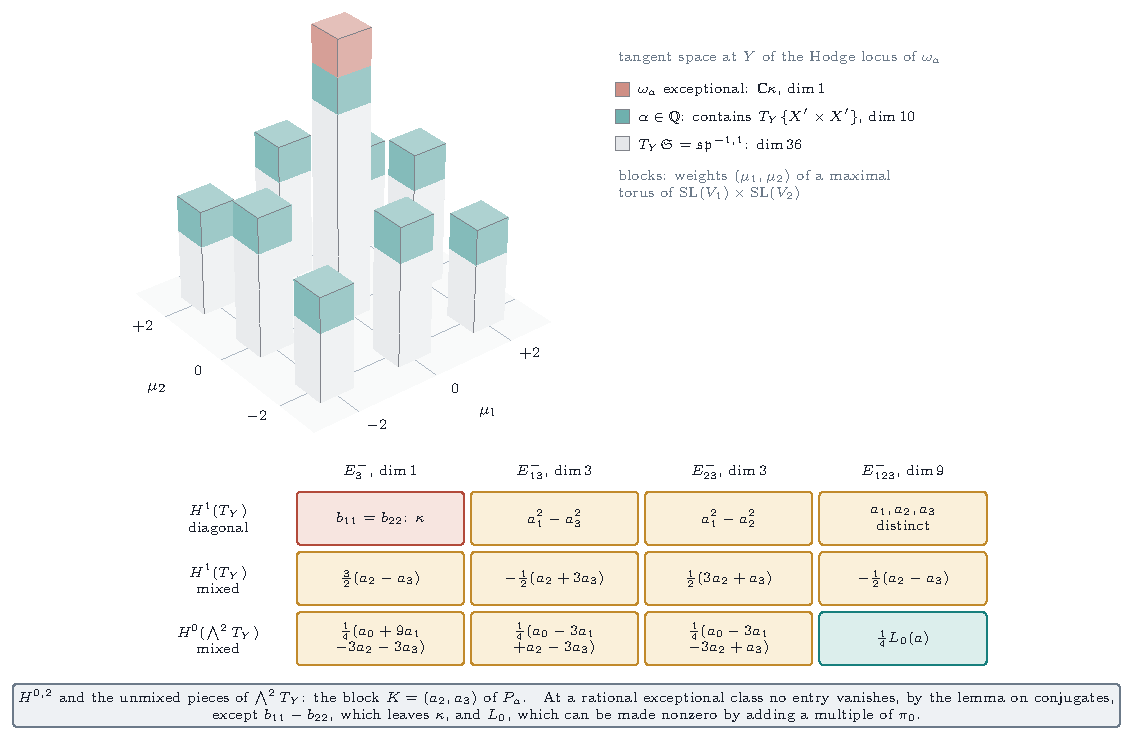
\includegraphics[width=\textwidth]{fig_rigidity}
\caption{\Cref{thm:mumfordrigid}. Top: the tangent space
$\mathfrak{sp}^{-1,1}$ of the Siegel space $\mathfrak{S}$ at
$Y=X_{c}\times X_{c}$, of dimension $36$, split into nine blocks by the
weights of a maximal torus of $\SL(V_{1})\times\SL(V_{2})$, one cube for each
dimension. The tangent space of the Hodge locus of an exceptional class is
the line $\CC\kappa$ of the Mumford curve, in the block of weight $(0,0)$;
for $\alpha\in\QQ$ it contains the tangent space of the diagonal Siegel space,
of dimension $10$ (\Cref{rem:rigidcompare}). Bottom: the scalars of Steps 4
to 6 of the proof on the pieces $E_{J}^{-}$ of $HT^{2}(Y)$; the pieces of
$H^{0,2}$ and the unmixed pieces of $H^{0}(\bigwedge^{2}T_{Y})$ are controlled
by the block $K$ of $P_{a}$ (Steps 3 and 4).}
\label{fig:rigidity}
\end{figure}

\begin{corollary}[No degeneration and no larger family]
\label{cor:nodegeneration}
Let $\omega$ be a rational exceptional class on $X_{c}\times X_{c}$. Every
connected complex analytic family of polarised abelian eightfolds through
$X_{c}\times X_{c}$ on which $\omega$ stays of Hodge type lies, near each
point of the curve, inside the curve $\{X_{t}\times X_{t}:t\in C\}$, which is
compact. In particular no such family degenerates, and on no member of it
other than the CM points of the curve is $\omega$ a combination of products
of divisor classes or of Weil classes of CM fields acting on the member or on
its quotients.
\end{corollary}

\begin{proof}
By \Cref{thm:mumfordrigid}(iii) the Hodge locus of $\omega$ coincides with the
curve in a neighbourhood of every point of the curve, so a connected family
through $Y$ on which $\omega$ stays of Hodge type maps into the curve near
each of its points over the curve; by connectedness and the identity theorem
its image lies in the curve. The curve is compact because $D$ is a division
algebra, so that the arithmetic group of the Shimura curve is cocompact
\cite{Mum69}. Indeed, by \Cref{setup:mumford} the algebra $D$ is definite at
$\sigma_{1}$ and $\sigma_{2}$, so $D\otimes_{F,\sigma_{1}}\RR$ is Hamilton's
quaternions and $D$ is not $M_{2}(F)$: it is a division algebra, split at the
one real place $\sigma_{3}$. The norm one group of an order in $D$, embedded
in $\SL_{2}(\RR)$ through $\sigma_{3}$, is a Fuchsian group of finite
covolume with no parabolic element, since a parabolic $\gamma\ne\pm1$ would
make $\gamma\mp1$ a nonzero nilpotent element of $D$; and a Fuchsian group of
finite covolume without parabolic elements has compact quotient.

For the last assertion: a member of the curve other than a CM point has
Hodge group $G$ (proof of \Cref{cor:mumfordequiv}), and on it $\omega$ lies
outside the span of the products of divisor classes and of the Weil classes
of quotients, by \Cref{prop:mumfordproduct}(ii) and (iii). At a CM point the
class is already algebraic (\Cref{thm:mumfordcm}), and the CM points, being
countably many, do not carry algebraicity to the other members
(\Cref{lem:spreading} needs uncountably many points).
\end{proof}

The same annihilator controls deformations that are not algebraic at all,
and so decides whether the twistor lines along which Markman moves sheaves
in his proof for Weil classes can be used here.

\begin{proposition}[The Hodge locus among all complex tori, and twistor
lines]\label{prop:notwistor}
Let $\omega$ be a rational exceptional class, $Y=X_{c}\times X_{c}$ with
$c\in C$, and $\Lambda=H_{1}(Y,\ZZ)$. Let $\mathcal{T}$ be the space of
complex structures on the real torus $\Lambda_{\RR}/\Lambda$, a complex
manifold of dimension $64$ with tangent space $H^{1}(T_{Y})$ at $Y$, and
$\mathcal{T}_{\omega}\subset\mathcal{T}$ the closed analytic subset on which
$\omega$ is of type $(2,2)$.
\begin{enumerate}[label=\textup{(\roman*)},leftmargin=2.6em,itemsep=2pt]
\item The connected component of $\mathcal{T}_{\omega}$ that contains $Y$ is
  the universal cover $\mathfrak{H}$ of the Mumford curve, the set of
  squares of members of the family, biholomorphic to the upper half plane.
  Every connected complex analytic family of complex tori, algebraic or not,
  through a member of the Mumford family on which $\omega$ stays of Hodge
  type lies in the family.
\item No twistor line through a member of the Mumford family, and no compact
  connected complex curve in $\mathcal{T}$ through it, keeps $\omega$ of
  Hodge type.
\item Nevertheless $\mathcal{T}_{\omega}$ contains twistor lines. The algebra
  $D\otimes_{F,\sigma_{1}}\RR$ is Hamilton's quaternions and acts on
  $V_{\RR}$ through the first factor of $G(\RR)$; for a unit quaternion $j$
  with $j^{2}=-1$, the complex structure $j\oplus j$ on $V_{\RR}\oplus
  V_{\RR}$ makes $\omega$ of type $(2,2)$, and these structures form a twistor
  line. On each factor $\psi(x,jy)$ has signature $(4,4)$, and a member whose
  Mumford--Tate group is $G$ is not an abelian variety. These twistor lines
  lie in components of $\mathcal{T}_{\omega}$ other than $\mathfrak{H}$.
\end{enumerate}
\end{proposition}

\begin{proof}
(i) The complex structures on $\Lambda_{\RR}$ for which all the tensors
invariant under $G$ are of Hodge type are those $J$ with $J^{2}=-1$ in the
real points of $G\cdot\mathbb{G}_{m}$, since a reductive group containing the
homotheties is the stabiliser of its invariant tensors. Let $\mathfrak{H}$ be
the connected component of this closed set that contains $Y$; it is closed in
$\mathcal{T}$ and consists of the $J=1\otimes1\otimes j_{3}$ with
$j_{3}\in\SL_{2}(\RR)$, $j_{3}^{2}=-1$, in the half plane that contains the
structure of $Y$, that is, of the squares of the members of the Mumford
family. At each of its points the first order condition for $\omega$ to stay
of type $(2,2)$ along $\xi\in H^{1}(T_{Y})$ is $\xi\lrcorner\,\omega=0$, as
in the proof of
\Cref{thm:mumfordrigid}(iii), where no polarisation was used, and by
\Cref{thm:mumfordrigid}(i) the solutions form the line $\CC\kappa$ tangent to
$\mathfrak{H}$. So near each of its points $\mathcal{T}_{\omega}$ is the smooth
curve germ of $\mathfrak{H}$, and $\mathfrak{H}$ is open in
$\mathcal{T}_{\omega}$. Being also closed and connected, it is a connected
component. A connected analytic family on which $\omega$ stays of Hodge type
maps into $\mathcal{T}_{\omega}$, hence into $\mathfrak{H}$ once one of its
points does.

(ii) A twistor line is a nonconstant holomorphic image of $\PP^{1}$ in
$\mathcal{T}$. If $\omega$ stayed of Hodge type along one through a point of
$\mathfrak{H}$, or along any compact connected curve through it, the curve
would lie in $\mathfrak{H}$ by (i), and a holomorphic map from a compact
connected curve to the upper half plane is constant.

(iii) At $\sigma_{1}$ the quaternion algebra $D$ is definite
(\Cref{setup:mumford}), so the first factor of $G(\RR)$ is the group of unit
quaternions, and $V_{\RR}$ restricted to it is a module over
$D\otimes_{F,\sigma_{1}}\RR\cong\mathbb{H}$. The unit quaternions $j$ with
$j^{2}=-1$ form a two-sphere, and the complex structures given by left
multiplication by them on a quaternionic vector space form a twistor line.
Each $j$ lies in $G(\RR)$, and so does the circle $\cos\vartheta+j\sin\vartheta$,
which fixes $\omega$; so $\omega$ is of type $(2,2)$. Inside
$V_{1}\otimes V_{2}\otimes V_{3}$ the space $V_{\RR}$ is the fixed space of a
real structure that is quaternionic on the first two factors and real on the
third, so $V_{\RR}=U\otimes V_{3,\RR}$ with $U$ the real form of
$V_{1}\otimes V_{2}$. On $U$ the form $g=\epsilon_{1}\otimes\epsilon_{2}$ is
symmetric and invariant under the compact group of pairs of unit quaternions,
which acts irreducibly on $U\otimes\CC=V_{1}\otimes V_{2}$; so $g$ is
definite. The complex structures of the Mumford family are $1\otimes h$, with
$h$ a complex structure on $V_{3,\RR}$ for which $\epsilon_{3}(\cdot,h\cdot)$
is definite, and $\psi(x,(1\otimes h)y)=g\otimes\epsilon_{3}(\cdot,h\cdot)$ is
definite. For $J=j\otimes1\otimes1$ the form $g(\cdot,(j\otimes1)\cdot)$ is
alternating, $j\otimes1$ being an isometry of $g$ with square $-1$, and
$\psi(x,Jy)=g(\cdot,(j\otimes1)\cdot)\otimes\epsilon_{3}$ is the product of
nondegenerate alternating forms on spaces of dimensions $4$ and $2$; as the
product of two alternating forms on $\RR^{2}$ is the determinant on
$\RR^{2}\otimes\RR^{2}=M_{2}(\RR)$, of signature $(2,2)$, it has signature
$(4,4)$. At a member whose Mumford--Tate group is $G$, the Hodge
classes of degree two on $V_{\RR}\oplus V_{\RR}$ are the forms $\psi\otimes s$
with $s$ a symmetric $2\times2$ matrix, by \Cref{prop:mumfordproduct}(ii), and
the signature of $\psi(\cdot,J\cdot)\otimes s$ is $(4(p+q),4(p+q))$ when $s$ has
signature $(p,q)$, so none is definite, none is a polarisation, and the member
is not an abelian variety. The members of the Mumford family are not on these
lines, since $\psi(x,Jy)$ is definite at the former and of signature $(4,4)$
at the latter, so by (i) the lines lie in other components.
\end{proof}

Markman's proof for Weil classes on abelian fourfolds moves a sheaf along
twistor lines on which its Chern character stays of Hodge type. By
\Cref{prop:notwistor} no such line passes through the square of a member of
the Mumford family: twistor lines on which $\omega$ is of Hodge type exist,
but they carry non-algebraic tori whose Hodge cocharacter lies in a definite
factor of $D$, and they lie in components of the Hodge locus that the Mumford
family never meets. The Kuga--Satake class of \Cref{thm:mumfordks} behaves
differently. The Kuga--Satake construction applies to every Hodge structure
of K3 type on $(T,q_{\lambda})$, so that class stays of Hodge type over the
whole period domain of $(T,q_{\lambda})$, of dimension seven, and not only
along the curve; among the classes attached to the target, it is the only one
for which deformation methods of this kind are not excluded.

The same space $T$ also makes the square a holomorphic symplectic variety,
and this determines what the mechanism of van Geemen and Rapagnetta would
have to supply here. They prove the Hodge conjecture for the general abelian
fourfold of Weil type with trivial discriminant by pulling back the second
Chern class of a hyperk\"ahler sixfold along a map from the fourfold, which
gives an algebraic class of codimension two that is not a product of divisor
classes \cite{vGR26}. For a projective hyperk\"ahler manifold $M$ write
$\sigma_{M}$ for its symplectic form, $q_{M}$ for its Beauville--Bogomolov
form and $T(M)$ for the orthogonal complement of $\NS(M)_{\QQ}$ in
$H^{2}(M,\QQ)$ for $q_{M}$.

\begin{proposition}[The square as a holomorphic symplectic
variety]\label{prop:hksquare}
Let $c\in C$ be a point at which the Mumford--Tate group of $X=X_{c}$ is
$G\cdot\mathbb{G}_{m}$, let $Y=X\times X$, and let $\Psi\in\bigwedge^{2}V$ be
the $G$-invariant bivector dual to $\psi$. For $x\in T$ put
$\iota(x)=(x\otimes1)\Psi$ in $V\otimes V=H^{1}(X,\QQ)\otimes H^{1}(X,\QQ)$, a
K\"unneth component of $H^{2}(Y,\QQ)$, and let $\iota_{2}\colon S^{2}T\to
H^{4}(Y,\QQ)$ be the map $xy\mapsto\iota(x)\cup\iota(y)$. Let $C_{i}\in
S^{2}T_{i}$ be the Casimir element of the trace form of
$\mathfrak{sl}(V_{i})$, and for $\nu\in F$ let
$c_{\nu}=\sum_{i}\sigma_{i}(\nu)C_{i}$, a rational element of $S^{2}T$; for
$\nu\ne0$ it is the element dual to the form $q_{1/\nu}$.
\begin{enumerate}[label=\textup{(\roman*)},leftmargin=2.6em,itemsep=2pt]
\item $\iota$ is an embedding of Hodge structures $T(-1)\to H^{2}(Y,\QQ)$, its
  image is the only irreducible sub-Hodge structure of $H^{2}(Y,\QQ)$ with
  $h^{2,0}=1$, and the holomorphic $2$-form $\sigma_{0}$ spanning its part of
  type $(2,0)$ is symplectic.
\item $\iota_{2}(c_{\nu})=\rho\,\omega_{a}$ with $a_{0}=3\Tr_{F/\QQ}(\nu)$ and
  $\alpha=4\nu-\Tr_{F/\QQ}(\nu)$, in the notation of \Cref{setup:omegaa},
  where $\rho$ is a nonzero rational number independent of $\nu$. So
  $\iota_{2}(c_{\nu})$ is exceptional if and only if $\nu\notin\QQ$, and every
  rational exceptional class is some $\iota_{2}(c_{\nu})$ plus a rational
  multiple of $\pi_{0}$.
\item Let $M$ be a projective hyperk\"ahler manifold and
  $f\colon Y\dashrightarrow M$ a rational map with $f^{*}\sigma_{M}\ne0$. Then
  $f^{*}$ maps $T(M)$ isomorphically onto $\iota(T)$ and is compatible with
  products of classes in $T(M)$; $f$ is generically finite onto a subvariety
  of dimension eight on which $\sigma_{M}$ is generically nondegenerate;
  $b_{2}(M)\ge10$; and $\dim M\ge10$.
\item Suppose in (iii) that $M=S^{[n]}$ is the Hilbert scheme of $n$ points
  on a projective K3 surface $S$, and
  let $q_{\lambda}$ be the form on $T$ that corresponds to the intersection
  form of $S$ on $T(S)=T(M)$ under $\iota^{-1}f^{*}$
  (\Cref{prop:mumfordrm}(iii)). If $\lambda\notin\QQ$, or if the real
  multiplication of $T(S)$ is induced by algebraic cycles on $S\times S$,
  then the Hodge conjecture holds for $Y$.
\end{enumerate}
\end{proposition}

\begin{proof}
(i) The map $\iota$ is $G$-equivariant because $\Psi$ is invariant, and
injective. Its image lies in $S^{2}V$: for $x$ in the symplectic Lie algebra
of $\psi$ one has $(x\otimes1)\Psi=-(1\otimes x)\Psi$, and the exchange of the
two factors carries $(x\otimes1)\Psi$ to $-(1\otimes x)\Psi=(x\otimes1)\Psi$,
because $\Psi$ is alternating. An element $g$ of $G\cdot\mathbb{G}_{m}$
multiplies $\Psi$ by the multiplier $\chi(g)$ of $\psi$, so $(g\otimes g)\iota(x)=
\chi(g)\,\iota(gxg^{-1})$: the map $\iota$ is equivariant for the adjoint
action on $T$ twisted by $\chi$, which is the action defining $T(-1)$. Both
Hodge structures come from the Hodge cocharacter through
$G\cdot\mathbb{G}_{m}$, so $\iota$ is a morphism of Hodge structures from
$T(-1)$. The sub-Hodge structures of $H^{2}(Y,\QQ)$ are its $G$-stable
subspaces, since $\mathbb{G}_{m}$ acts by scalars. Over $\bar{\QQ}$,
$H^{2}(Y)=\bigwedge^{2}(V\otimes\bar{\QQ}^{2})=S^{2}V\oplus(\bigwedge^{2}V)^{\oplus3}$,
and expanding $V\otimes V=\bigotimes_{k}(S^{2}V_{k}\oplus\bigwedge^{2}V_{k})$
gives $\bigwedge^{2}V$ as the sum of the pieces of highest weights $(0,0,0)$,
$(2,2,0)$, $(2,0,2)$, $(0,2,2)$ (an odd number of factors $\bigwedge^{2}V_{k}$)
and $S^{2}V$ as the sum of those of highest weights $(2,2,2)$, $(2,0,0)$,
$(0,2,0)$, $(0,0,2)$. So the isotypic pieces of $H^{2}(Y)$ have these eight
highest weights and dimensions $3,27,27,27,27,3,3,3$. The Hodge cocharacter
acts through $V_{3}$, on which it has one weight of each type, so $S^{2}V_{3}$
has one dimension of type $(2,0)$ and $\bigwedge^{2}V_{3}$ none; the parts of
type $(2,0)$ of the eight pieces have dimensions $0,0,9,9,9,0,0,1$. The last
three pieces occur once, in $S^{2}V$, and are $\iota(T_{1})$, $\iota(T_{2})$,
$\iota(T_{3})$. So an irreducible summand of highest weight $(2,0,2)$ or
$(0,2,2)$ contributes $3$ to $h^{2,0}$, one of weight $(2,2,2)$ contributes
$9$, one of weight $(0,0,2)$ contributes $1$, and the others contribute
nothing. A rational sub-Hodge structure $W$ is stable under the Galois group,
which permutes the highest weights as it permutes the factors, transitively.
So if $W\otimes\bar{\QQ}$ has a summand of weight $(2,2,0)$, $(2,0,2)$ or
$(0,2,2)$, it has summands of all three and $h^{2,0}(W)\ge6$; if it has one of
weight $(2,2,2)$, then $h^{2,0}(W)\ge9$. If $h^{2,0}(W)=1$, therefore,
$W\otimes\bar{\QQ}$ contains the piece $\iota(T_{3})$ of weight $(0,0,2)$,
which has multiplicity one, and with it $\iota(T_{1})$ and $\iota(T_{2})$; so
$W\supseteq\iota(T)$, and $W=\iota(T)$ if $W$ is irreducible. The same
argument shows that $\iota(T)$ is irreducible: a nonzero sub-Hodge structure
of it contains one of the $\iota(T_{i})$ over $\bar{\QQ}$, hence all three.
The part of type $(2,0)$ of $\iota(T)$ is spanned by $\sigma_{0}=\iota(E_{3})$,
where $E_{3}\in\mathfrak{sl}(V_{3})\otimes\CC$ maps $V_{3}^{0,1}$ onto
$V_{3}^{1,0}$. Write $\Psi=\Psi_{1}\otimes\Psi_{2}\otimes\Psi_{3}$ with
$\Psi_{k}\in\bigwedge^{2}V_{k}$ dual to $\epsilon_{k}$, and
$\Psi_{3}=e_{+}\otimes e_{-}-e_{-}\otimes e_{+}$ with $e_{\pm}$ spanning
$V_{3}^{1,0}$ and $V_{3}^{0,1}$. Then $(E_{3}\otimes1)\Psi_{3}$ is a nonzero
multiple of $e_{+}\otimes e_{+}$, so $\sigma_{0}$ is a nonzero multiple of
$\Psi_{1}\otimes\Psi_{2}\otimes e_{+}\otimes e_{+}$: it lies in
$H^{1,0}(X)\otimes H^{1,0}(X)$ and pairs $H^{1,0}$ of the first factor with
$H^{1,0}$ of the second through the nondegenerate form dual to
$\epsilon_{1}\otimes\epsilon_{2}$ on $V_{1}\otimes V_{2}$. So $\sigma_{0}$ has
rank eight: it is a holomorphic symplectic form on $Y$.

(ii) For $x,y\in T$ the class $\iota(x)\cup\iota(y)$ lies in
$H^{2}(X)\otimes H^{2}(X)$ and comes from the tensor
$(x\otimes1)\Psi\otimes(y\otimes1)\Psi$ in $V^{\otimes4}$ by antisymmetrising
its two slots in the first factor of $Y$ and its two slots in the second.
Read it, as in \Cref{setup:omegaa}, as a map from the first-factor slots to
the second-factor slots. Contraction with $\epsilon_{k}$ turns
$\Psi_{k}\otimes\Psi_{k}$ into $\gamma$ times the identity of
$V_{k}\otimes V_{k}$ and, for $x,y\in T_{k}$, the tensor
$(x\otimes1)\Psi_{k}\otimes(y\otimes1)\Psi_{k}$ into $\gamma\,(x\otimes y)$,
with one and the same constant $\gamma\ne0$, since $x$ and $y$ are
antisymmetric for $\epsilon_{k}$ and the two signs cancel. So $\iota_{2}(C_{1})$
corresponds, up to a nonzero constant $\gamma'$ independent of the factor, to
the restriction to $\bigwedge^{2}V$ of $\mathrm{Cas}_{1}\otimes1\otimes1$,
where $\mathrm{Cas}_{1}=\sum_{c}x_{c}\otimes x^{c}=s_{1}-\frac12$ is the
operator of Step 3 of the proof of \Cref{thm:mumfordpowers}, $s_{1}$ the
exchange of the two copies of $V_{1}$. On $\bigwedge^{2}V$ the exchange
$s_{1}$ is $-1$ on $\QQ\theta$ and $U_{23}$ and $+1$ on $U_{12}$ and $U_{13}$,
so $\iota_{2}(C_{1})=\rho\,(3\pi_{0}-\pi_{12}-\pi_{13}+3\pi_{23})$ with
$\rho=-2\gamma'$, and permuting the factors gives the two cyclic permutations
of this identity. Summing with the coefficients $\sigma_{i}(\nu)$ gives
$\iota_{2}(c_{\nu})=\rho\bigl(3\Tr(\nu)\pi_{0}+\sum\sigma_{k}(4\nu-\Tr(\nu))
\pi_{ij}\bigr)$, the sum over $\{i,j,k\}=\{1,2,3\}$ with $i<j$, which is
$\rho\,\omega_{a}$ with the stated $a_{0}$ and $\alpha$. For rational $\nu\ne0$
both $\iota_{2}(c_{\nu})$ and $\omega_{a}$ are rational and nonzero, so
$\rho\in\QQ$. Since
$\Tr(\nu)\in\QQ$, the element $\alpha$ is rational exactly when $\nu$ is; and
$\Tr(\alpha)=\Tr(\nu)$, so $\nu=(\alpha+\Tr(\alpha))/4$ recovers $\nu$ from
any $\alpha\in F$. Two rational classes with the same $\alpha$ differ by a
multiple of $\pi_{0}$, and $\iota_{2}(c_{\nu/\rho})=\omega_{a}$ because
$c_{\nu}$ is linear in $\nu$; so every rational exceptional class is some
$\iota_{2}(c_{\nu})$ plus a rational multiple of $\pi_{0}$. The Casimir element $C_{i}$ is dual to the trace form
on $T_{i}$, so $c_{\nu}$ is dual to $\sum_{i}\sigma_{i}(\nu)^{-1}
\operatorname{tr}(x_{i}y_{i})=q_{1/\nu}(x,y)$.

(iii) Resolve the indeterminacy of $f$ by a sequence of blow-ups along
smooth centres, $\pi\colon\tilde{Y}\to Y$ and $\tilde{f}\colon\tilde{Y}\to M$,
and put $f^{*}=\pi_{*}\tilde{f}^{*}$, a morphism of Hodge structures. The
kernel of $\pi_{*}$ on $H^{2}(\tilde{Y},\QQ)$ is spanned by the classes of
the exceptional divisors, so $\alpha\mapsto\tilde{f}^{*}\alpha-
\pi^{*}f^{*}\alpha$ is a morphism of Hodge structures from $H^{2}(M,\QQ)$ to a
space of Hodge classes. The Hodge structure $T(M)$ is irreducible: a
sub-Hodge structure $W\subseteq T(M)$ with $W^{2,0}=0$ consists of rational
classes of type $(1,1)$, which lie in $\NS(M)_{\QQ}\cap T(M)=0$; if
$W^{2,0}\ne0$, then $\sigma_{M}\in W_{\CC}$, the orthogonal complement of $W$
in $H^{2}(M,\QQ)$ is a sub-Hodge structure orthogonal to $\sigma_{M}$ and
$\bar{\sigma}_{M}$, hence of type $(1,1)$ and contained in $\NS(M)_{\QQ}$,
and $W\supseteq T(M)$. Since $T(M)$ is not spanned by Hodge classes, that
morphism vanishes on it, and $\tilde{f}^{*}\alpha=\pi^{*}f^{*}\alpha$ for
$\alpha\in T(M)$. Because $\tilde{f}^{*}$ is a ring homomorphism and
$\pi_{*}\pi^{*}$ is the identity, $f^{*}(\alpha\beta)=f^{*}\alpha\cup
f^{*}\beta$ for $\alpha,\beta\in T(M)$. The kernel of $f^{*}$ on $T(M)$ is a
sub-Hodge structure not containing $\sigma_{M}$, hence zero, and the image is
irreducible with $h^{2,0}=1$, hence $\iota(T)$ by (i). So $f^{*}\sigma_{M}$ is
a nonzero multiple of $\sigma_{0}$ and has rank eight at every point of $Y$
where $f$ is defined; the rank of a pulled-back form is at most the dimension
of the image, so $f$ is generically finite onto its image $Z$, of dimension
eight, and $\sigma_{M}$ is generically nondegenerate on $Z$. As $M$ is
projective, $b_{2}(M)=\dim T(M)+\dim\NS(M)_{\QQ}\ge9+1$; this excludes the
generalised Kummer varieties, whose second Betti number is seven
\cite{Bea83}. Finally $\dim M\ge\dim Z=8$; suppose that $\dim M=8$. Then
$f$ is dominant, and for $\alpha\in T(M)_{\CC}$ the relation of Fujiki and
Beauville \cite{Bea83,Fuj87} gives
\[
  \int_{Y}(f^{*}\alpha)^{8}=\int_{\tilde{Y}}\tilde{f}^{*}(\alpha^{8})
  =\deg(f)\int_{M}\alpha^{8}=\deg(f)\,c_{M}\,q_{M}(\alpha)^{4},
  \qquad c_{M}>0 .
\]
Write $f^{*}\alpha=\iota(x)$ with $x=x_{1}+x_{2}+x_{3}\in T_{\CC}$ and
$N_{i}=-\det x_{i}$. The form $x\mapsto q_{M}((f^{*})^{-1}\iota(x))$ is
invariant under $G$, so it is $q_{\lambda}(x,x)=
\sum_{i}\sigma_{i}(\lambda)\operatorname{tr}(x_{i}^{2})=
2\sum_{i}\sigma_{i}(\lambda)N_{i}$ for some $\lambda\in F^{\times}$ by
\Cref{prop:mumfordrm}(iii). On the other side, in a basis $(e_{i})$ of
$V$ one has $\iota(x)=\sum_{i,j}M_{ij}\,e_{i}^{(1)}\wedge e_{j}^{(2)}$, with
$M$ the product of the matrix of $x$ and the constant invertible matrix of
$\Psi$, and the $2$-forms $e_{i}^{(1)}\wedge e_{j}^{(2)}$ commute, so
$\iota(x)^{8}=8!\det(M)\prod_{i}e_{i}^{(1)}\wedge e_{i}^{(2)}$ is $8!\det(x)$
times a fixed volume form, and
$\det(x_{1}\otimes1\otimes1+1\otimes x_{2}\otimes1+1\otimes1\otimes
x_{3})=\Delta(N_{1},N_{2},N_{3})^{2}$ with
$\Delta=N_{1}^{2}+N_{2}^{2}+N_{3}^{2}-2N_{1}N_{2}-2N_{1}N_{3}-2N_{2}N_{3}$;
this is also the product of the eight numbers $\pm r_{1}\pm r_{2}\pm r_{3}$,
where $\pm r_{i}$ are the eigenvalues of $x_{i}$ and $r_{i}^{2}=N_{i}$. The
$N_{i}$ are algebraically independent functions on $T_{\CC}$, so the two
expressions for $\int_{Y}(f^{*}\alpha)^{8}$ would make $\Delta^{2}$ a nonzero
constant multiple of the fourth power of the linear form
$\sum_{i}\sigma_{i}(\lambda)N_{i}$, and then, by unique factorisation,
$\Delta$ a multiple of its square. But $\Delta$ is a nondegenerate
ternary quadratic form, hence irreducible. So $\dim M\ne8$, and since the
dimension of a hyperk\"ahler manifold is even, $\dim M\ge10$.

(iv) By \cite{Bea83} the map $H^{2}(S,\QQ)\to H^{2}(S^{[n]},\QQ)$ induced by
the universal subscheme $Z_{n}\subset S\times S^{[n]}$ is injective, carries
the intersection form to the Beauville--Bogomolov form, and has
$H^{2}(S^{[n]},\QQ)=H^{2}(S,\QQ)\oplus\QQ\delta$ with $\delta$ algebraic, so
$T(M)=T(S)$. Let $\Delta_{T}$ be the K\"unneth component in $T(S)\otimes
T(S)$ of the class of the diagonal of $S$; it is algebraic, being the class
of the diagonal minus $[\mathrm{pt}\times S]$, $[S\times\mathrm{pt}]$ and
$\sum_{r}d_{r}\times d_{r}^{\vee}$ over dual bases of $\NS(S)_{\QQ}$. Its image
under the correspondence $Z_{n}\times Z_{n}$, pulled back along the diagonal
of $M$, is the class $\sum_{a}e_{a}\cup e_{a}^{\vee}$ over dual bases of
$T(S)$ for the intersection form, which is therefore algebraic on $M$, and by
(iii) its image under $f^{*}$ is $\iota_{2}$ of the element of $S^{2}T$ dual
to $q_{\lambda}$, that is $\iota_{2}(c_{1/\lambda})$, an algebraic class on
$Y$. If $\lambda\notin\QQ$ it is exceptional by (ii). If instead the real
multiplication is algebraic, apply it to the first factor of $\Delta_{T}$:
for $b\in F$ the class $\sum_{a}(m_{b}e_{a})\cup e_{a}^{\vee}$ is algebraic,
and its image is $\iota_{2}(c_{b/\lambda})$, which is exceptional for
$b\notin\QQ\lambda$. In both cases \Cref{lem:oneexceptional} makes every
Hodge class in $H^{2}(X)\otimes H^{2}(X)$ algebraic; the Hodge classes in the
other K\"unneth components of $H^{4}(Y,\QQ)$ are products of divisor classes,
as at the end of the proof of \Cref{thm:mumfordks}; and the Hodge classes of
$Y$ form a ring generated in degrees two and four (proof of
\Cref{cor:mumfordequiv}). So every Hodge class of $Y$ is algebraic.
\end{proof}

\begin{remark}[The mechanism of van Geemen and
Rapagnetta]\label{rem:hkroute}
By \Cref{prop:hksquare}(ii) the exceptional classes are, up to rational
multiples of $\pi_{0}$, the classes $\iota_{2}(c_{\nu})$ with $\nu\notin\QQ$,
the images of the elements dual to the forms $q_{\lambda}$, $\lambda=1/\nu$,
on the part $\iota(T)$ of $H^{2}(Y)$ generated by the symplectic class; the
form with $\lambda$ rational gives a product of divisor classes. They are the
analogues for $(Y,\sigma_{0})$ of the dual Beauville--Bogomolov class, whose
pull-back is what \cite{vGR26} uses. By part (iii), a transfer of that
argument needs a projective hyperk\"ahler manifold of dimension at least ten with
transcendental part $T(-1)$, such as $S_{\mu}^{[n]}$ with $n\ge5$ for a
surface $S_{\mu}$ of \Cref{thm:mumfordks}, and a rational map from $Y$ onto a
symplectic subvariety of dimension eight. For $M=S_{\mu}^{[n]}$ the form of
(iv) is $q_{\mu/e^{2}}$ for the $e\in F^{\times}$ with $\iota^{-1}f^{*}=m_{e}$
on $T(S_{\mu})=T$, so $\lambda\notin\QQ$ for every such map as soon as
$\mu\notin\QQ^{\times}F^{\times2}$. No such map is known. It would give an
algebraic cycle on $S_{\mu}\times X\times X$ inducing an isomorphism of
$T(S_{\mu})$ onto $\iota(T)\subset H^{1}(X)\otimes H^{1}(X)$, a correspondence
of the kind that the Kuga--Satake class supplies in the proof of
\Cref{thm:mumfordks}; so this route is the Kuga--Satake route in geometric
form rather than an independent one. By (iii), maps to K3 surfaces and to
hyperk\"ahler eightfolds cannot serve.
\end{remark}

\begin{theorem}[A numerical criterion for the Mumford classes]
\label{thm:mumfordnumerical}
Let $c\in C$, $Y=X_{c}\times X_{c}$, $\omega=\omega_{a}$ a rational
exceptional class with $L_{0}(a)\ne0$, and $E$ a perfect complex on $Y$ with
$\ch(E)=N\omega$, $N\ne0$, and no other component.
\begin{enumerate}[label=\textup{(\roman*)},leftmargin=2.6em,itemsep=2pt]
\item $\dim\Ext^{2}(E,E)\ge119$.
\item If $\dim\Ext^{2}(E,E)=119$, then $\operatorname{ev}_{E}\colon
  HT^{2}(Y)\to\Ext^{2}(E,E)$ is surjective with kernel $\CC\kappa$, and
  $\sigma_{E}$ is injective. Conversely, if $\sigma_{E}$ is injective, then
  $\operatorname{ev}_{E}$ has rank $119$ and kernel $\CC\kappa$, and $E$
  extends to first order along the curve.
\item If some such $E$ at one point $c$ has $\dim\Ext^{2}(E,E)=119$, then
  $\omega_{t}$ is algebraic for every $t\in C$, the Hodge conjecture holds for
  $X_{t}\times X_{t}$ for every $t$, and $B(W\times_{C}W)$ holds.
\item At every CM point $c$ some perfect complex $E$ on $Y$ has
  $\ch(E)=N\omega$ for some $N\ne0$ and no other component.
\end{enumerate}
\end{theorem}

\begin{proof}
(i) and (ii). By the square $\sigma_{E}\circ\operatorname{ev}_{E}=
(\,\cdot\,)\lrcorner\,\ch(E)$ of \cite[Setup~4.54]{paperII}, $\ker
\operatorname{ev}_{E}\subseteq\Ann_{HT^{2}}(\omega)=\CC\kappa$ by
\Cref{thm:mumfordrigid}(ii), so $\operatorname{ev}_{E}$ has rank at least
$119$, which is (i). If $\dim\Ext^{2}(E,E)=119$, then
$\operatorname{ev}_{E}$ is onto, its kernel has dimension one and lies in
$\CC\kappa$, so equals it; and $\sigma_{E}(\operatorname{ev}_{E}(x))=
N\,x\lrcorner\,\omega$ vanishes only for $x\in\CC\kappa=\ker
\operatorname{ev}_{E}$, so $\sigma_{E}$ is injective on
$\image\operatorname{ev}_{E}=\Ext^{2}(E,E)$. Conversely, if $\sigma_{E}$ is
injective, then $\sigma_{E}(\operatorname{ev}_{E}(\kappa))=N\kappa\lrcorner
\,\omega=0$ forces $\operatorname{ev}_{E}(\kappa)=0$, so the kernel is
$\CC\kappa$ and the rank is $119$; and $\operatorname{ev}_{E}$ restricted to
$H^{1}(T_{Y})$ is the obstruction map \cite{Tod09}, which therefore vanishes
at $\kappa$, so that $E$ extends to first order along the curve.

(iii) By (ii) $\sigma_{E}$ is injective. The Chern character of $E$ is
$N\omega$, a flat section of Hodge type over the whole of $C$, so
\cite[Theorem~2.2]{paperII} applies to every infinitesimal deformation of $Y$ inside
$W\times_{C}W\to C$. The proof of \cite[Theorem~2.3]{paperII} then applies word
for word, with the stack of perfect complexes on the fibres of $W\times_{C}
W\to C$ \cite{Lie06} in place of that of $\cA\to\cS$, or the analytic
Kuranishi germ if $\Ext^{<0}(E,E)\ne0$: it is smooth over $C$ at $[E]$, its
image contains a nonempty open subset $U\subseteq C$, and for $t\in U$ a
perfect complex $E_{t}$ on $X_{t}\times X_{t}$ in the same connected
component has $\ch(E_{t})=N\omega_{t}$, so $\omega_{t}$ is algebraic, and by
\Cref{lem:oneexceptional} so are both exceptional classes. Since $U$ is
uncountable, \Cref{cor:mumfordequiv} gives the rest.

(iv) By \Cref{thm:mumfordcm} there is $\xi\in\CH^{2}(Y)_{\QQ}$ with class
$\omega$, and the argument of \cite[Proposition~2.1]{paperII} gives $E$: the Chern
character is an isomorphism $K_{0}(Y)_{\QQ}\to\CH^{*}(Y)_{\QQ}$
\cite[Ex.~15.2.16(b) and Cor.~18.3.2]{Ful98}, so $\xi=\ch(u)$ for a unique
$u$, and $Nu$ is the class of a perfect complex for a suitable $N$.
\end{proof}

Part (iii) is the Mumford analogue of \cite[Theorem~2.11(iii)]{paperII}: one object,
at one point, and one number, which is $119$ here and $2n(2n-1)$ for a Weil
family. For a Weil family that number is attained by no object
(\cite[Theorem~3.5]{paperII}), because an object attaining it would have to deform to
non-algebraic tori; the classes here are rigid, so that argument does not
apply (\cite[Remark~3.6]{paperII}). The objects of (iv) exist, and the criterion
asks that one of them, or another representative of the same class in
$K_{0}$, attain the bound of (i). The rigidity of \Cref{thm:mumfordrigid} is no obstacle:
semiregularity moves an object along the Hodge locus of its Chern character,
and the curve is exactly that locus, so a semiregular object would propagate
along the curve and nowhere else, which is all that is needed.

\begin{corollary}[Bounded data at CM points]\label{cor:mumfordbounded}
Fix a relatively ample line bundle on $W\times_{C}W\to C$, and let $\omega$ be
a rational exceptional class. The following are equivalent.
\begin{enumerate}[label=\textup{(\alph*)},leftmargin=2.6em,itemsep=2pt]
\item $\omega_{t}$ is algebraic for every $t\in C$; equivalently, by
  \Cref{lem:oneexceptional} and \Cref{cor:mumfordequiv}, the Hodge conjecture
  holds for $X_{t}\times X_{t}$ for every $t\in C$.
\item There are a finite set $\Phi$ of pairs $(\underline{P},\underline{q})$,
  each a tuple of Hilbert polynomials with a tuple of rational numbers of the
  same length, and infinitely many points $c\in C$ at each of which
  $\omega_{c}=\sum_{i}q_{i}[Z_{i}]$ for subschemes $Z_{i}\subset X_{c}\times
  X_{c}$ with Hilbert polynomials $P_{i}$, for some $(\underline{P},
  \underline{q})\in\Phi$.
\end{enumerate}
In particular the classes are algebraic on every member as soon as they are
represented at infinitely many CM points by cycles of bounded degree.
\end{corollary}

\begin{proof}
For a pair $(\underline{P},\underline{q})$ let $\Sigma_{\underline{P},
\underline{q}}\subseteq C$ be the set of points at which $\omega$ is
represented with these data. The proof of \cite[Theorem~16.4]{paperI} applies
verbatim to $(W\times_{C}W,C,\omega)$, as in \Cref{lem:spreading}, and shows
that each $\Sigma_{\underline{P},\underline{q}}$ is Zariski closed. If (b)
holds, then, $\Phi$ being finite, one pair of $\Phi$ serves at infinitely
many points, so its $\Sigma$ is an infinite closed subset of the irreducible
curve $C$, hence $C$, and (a) holds. If (a) holds, $C$ is the union of the
countably many $\Sigma_{\underline{P},\underline{q}}$, and $C$ is
uncountable, so one of
them is infinite, hence equal to $C$; then (b) holds with $\Phi$ that one
pair and every point of $C$.
\end{proof}

The proof of \Cref{thm:mumfordcm} represents the classes at every CM point,
through Markman's theorem for abelian fourfolds \cite{Mar25a} and the ring
generated by divisor classes and pull-backs of Hodge classes of $X_{c}$ along
homomorphisms $X_{c}\times X_{c}\to X_{c}$, but with no control of degree;
isogenies between CM members, which move CM points along their Hecke orbits,
do not bound the degree either. By
\Cref{cor:mumfordbounded} such a bound, at infinitely many CM points, is
equivalent to the target; without it the CM points, being countably many,
say nothing about a very general member (\Cref{lem:spreading} needs
uncountably many points).

The next proposition says which endomorphisms those pull-backs have to use.
At a CM point the fourfold is of Weil type, its two Hodge classes of degree
four that are not products of divisor classes form its Weil line, and the
exceptional classes of the square are out of reach of everything built from
that line with the Weil field alone: they need the real multiplication by the
totally real quartic algebra of Rosati-fixed endomorphisms, and all of it.

\begin{proposition}[The Weil structure at a CM point, and what the cycles
must use]\label{prop:cmsource}
Let $c\in C$ be a CM point, $X=X_{c}$, $Y=X\times X$, and let $e_{w}$,
$w\in\{\pm1\}^{3}$, be a weight basis of $V=H^{1}(X,\CC)$ for the Hodge torus
$T$ of $X$, as in the proof of \Cref{thm:mumfordcm}, normalised so that
$\psi(e_{w},e_{-w})=\pm1$, with $e^{(1)}_{w}$, $e^{(2)}_{w}$ its two copies in
$H^{1}(Y,\CC)$. Let $T_{+}$ be the set of the four weights with an even
number of entries $-1$, let $T_{-}=-T_{+}$ be the set of the other four, let
$t_{\pm}=\prod_{w\in T_{\pm}}e_{w}\in H^{4}(X,\CC)$, the factors in a fixed
order, and let $\dagger$ be the Rosati involution of $\theta$ on
$\End^{0}(X)$. For $\varphi\in\End^{0}(X)$ write $\varphi_{w}$ for its
eigenvalue on $e_{w}$.
\begin{enumerate}[label=\textup{(\roman*)},leftmargin=2.6em,itemsep=2pt]
\item $T_{+}$ and $T_{-}$ are the only sets of four weights with sum zero
  that contain no pair of opposite weights, and $\Hdg^{2}(X)\otimes\CC$ is
  the direct sum of the span of the products of divisor classes and of
  $\CC t_{+}\oplus\CC t_{-}$. The elements of $\End^{0}(X)$ with
  $\varphi_{w}$ constant on $T_{+}$ and constant on $T_{-}$ form an imaginary
  quadratic field $k_{c}$; $(X,k_{c},\theta)$ is of $(k_{c},-1,2)$-Weil type,
  and its Weil line is $\HW(X)=(\CC t_{+}\oplus\CC t_{-})\cap H^{4}(X,\QQ)$.
  The fixed algebra $K_{c}^{+}$ of $\dagger$ consists of the elements with
  $\varphi_{w}=\varphi_{-w}$ for every $w$; it is a product of totally real
  fields of total degree four, and $\End^{0}(X)=K_{c}^{+}\otimes_{\QQ}k_{c}$.
\item For $\varphi,\psi\in\End^{0}(X)$ let $f_{\varphi,\psi}^{*}$ be the ring
  homomorphism $H^{*}(X,\QQ)\to H^{*}(Y,\QQ)$ that sends $e\in H^{1}(X,\QQ)$
  to $\mathrm{pr}_{1}^{*}\varphi^{*}e+\mathrm{pr}_{2}^{*}\psi^{*}e$; for
  $\varphi,\psi\in\End(X)$ it is the pull-back along the homomorphism
  $\varphi\circ\mathrm{pr}_{1}+\psi\circ\mathrm{pr}_{2}\colon Y\to X$, and
  every homomorphism $Y\to X$ is of this form. For a $\QQ$-subalgebra
  $R\subseteq\End^{0}(X)$ let $\Sigma_{R}\subseteq\Hdg^{2}(Y)$ be the
  $\QQ$-span of the products of two divisor classes of $Y$ and of the classes
  $f_{\varphi,\psi}^{*}\HW(X)$ with $\varphi,\psi\in R$. Then
  $\Sigma_{k_{c}}=\Sigma_{\QQ}$, the span obtained from the maps
  $(x,y)\mapsto ax+by$ alone, has dimension $110$ and meets the span of
  $\pi_{0},\pi_{12},\pi_{13},\pi_{23}$ in the plane of the classes with
  $a_{1}=a_{2}=a_{3}$; it contains no exceptional class.
\item For a $\QQ$-subalgebra $R\subseteq\End^{0}(X)$ the following are
  equivalent: \textup{(a)} $\Sigma_{R}$ contains an exceptional class;
  \textup{(b)} $\Sigma_{R}=\Hdg^{2}(Y)$, which has dimension $132$;
  \textup{(c)} $R$ separates the weights of $T_{+}$, that is, for any two
  distinct $w,w'\in T_{+}$ some $\varphi\in R$ has
  $\varphi_{w}\ne\varphi_{w'}$; equivalently, $R$ and $k_{c}$ generate
  $\End^{0}(X)$. In particular $\Sigma_{K_{c}^{+}}=\Hdg^{2}(Y)$, while
  $\Sigma_{R}$ contains no exceptional class if $R$ is a proper subalgebra
  of $K_{c}^{+}$ or a subalgebra of $k_{c}$.
\end{enumerate}
\end{proposition}

\begin{proof}
(i) The four weights $d_{1}=(1,1,1)$, $d_{2}=(1,-1,-1)$, $d_{3}=(-1,1,-1)$,
$d_{4}=(-1,-1,1)$ of $T_{+}$ have sum zero, and any three of them are
linearly independent, so every linear relation among them is a multiple of
$d_{1}+d_{2}+d_{3}+d_{4}=0$. A set of four weights containing no opposite
pair contains exactly one of $d_{i}$, $-d_{i}$ for each $i$, say
$\varepsilon_{i}d_{i}$, and has sum zero only if
$\sum_{i}\varepsilon_{i}d_{i}=0$, that is, if all $\varepsilon_{i}$ are
equal: the set is $T_{+}$ or $T_{-}$. The Hodge classes of $X$ of degree
four, tensored with $\CC$, are spanned by the monomials $\prod_{w\in S}e_{w}$
over the sets $S$ of four weights with sum zero (proof of
\Cref{thm:mumfordcm}); the divisor classes are spanned by the four monomials
$e_{w}e_{-w}$ of weight zero and degree two, their products are the six
monomials of the sets that are unions of two opposite pairs, and the two
remaining sets are $T_{+}$ and $T_{-}$.

The torus $T$ is defined over $\QQ$, so the Galois group of $\bar{\QQ}$ acts
linearly on its character lattice and permutes the set of the eight weights
of $V$. A linear map that permutes the weights carries opposite pairs to
opposite pairs and sets with sum zero to sets with sum zero, hence carries
$\{T_{+},T_{-}\}$ to itself. Over $\bar{\QQ}$ the algebra
$\End^{0}(X)\otimes\bar{\QQ}=\End_{T}(V_{\bar{\QQ}})$ consists of the
diagonal matrices $\sum_{w}x_{w}p_{w}$ in the weight basis, $p_{w}$ the
projection to the weight space of $w$, and $\gamma\in\Gal(\bar{\QQ}/\QQ)$
acts by $\gamma(\sum_{w}x_{w}p_{w})=\sum_{w}\gamma(x_{w})p_{\gamma w}$,
because $\gamma$ carries the weight space of $w$ to that of $\gamma w$. As
$\psi$ is $T$-invariant, $\psi(e_{w},e_{w'})=0$ unless $w'=-w$, so the
adjoint of $\sum_{w}x_{w}p_{w}$ for $\psi$, which is the Rosati involution,
is $\sum_{w}x_{-w}p_{w}$. The subalgebra $A_{W}$ of the diagonal matrices
that are constant on $T_{+}$ and on $T_{-}$, and the subalgebra $A^{+}$ of
those with $x_{w}=x_{-w}$ for all $w$, are therefore stable under the Galois
group and under $\dagger$; so $k_{c}=A_{W}\cap\End^{0}(X)$ and
$K_{c}^{+}=A^{+}\cap\End^{0}(X)$ are $\QQ$-forms of $A_{W}$ and $A^{+}$, of
dimensions $2$ and $4$, and $K_{c}^{+}$ is the fixed algebra of $\dagger$.
On $A_{W}$ the involution $\dagger$ exchanges the two scalars. The Rosati
involution is positive: $\Tr(xx^{\dagger})>0$ for $x\ne0$, with $\Tr$ the
trace on $V$ \cite[Section~5.1]{BL04}. If $k_{c}$ were not a field it would
contain the idempotent $p_{+}=\sum_{w\in T_{+}}p_{w}$, and
$\Tr(p_{+}p_{+}^{\dagger})=\Tr(p_{+}p_{-})=0$; so $k_{c}$ is a quadratic
field on which $\dagger$ is the nontrivial automorphism. If $k_{c}$ were
real, $x=\sqrt{d}\in k_{c}$ would satisfy $x^{\dagger}=-x$ and
$\Tr(xx^{\dagger})=-\Tr(x^{2})=-8d<0$. So $k_{c}$ is imaginary quadratic and
$\dagger$ is complex conjugation on it, which is condition (iii) of
\cite[Definition~3.1]{paperI}. The eigenspaces of $k_{c}\otimes\CC$ on $V$ are
$V_{\pm}=\bigoplus_{w\in T_{\pm}}\CC e_{w}$. The Hodge decomposition of $V$
is the eigenspace decomposition of the Hodge cocharacter, which takes values
in the diagonal torus $T_{\CC}\cdot\mathbb{G}_{m}$, so every $e_{w}$ is of
pure type $(1,0)$ or $(0,1)$, and $t_{+}$ is of type $(p,4-p)$ with
$p=\dim(V_{+}\cap H^{1,0}(X))$. Since $t_{+}$ is a Hodge class, $p=2$: each
eigenvalue of $\sqrt{-d}$ has multiplicity two on $H^{1,0}(X)$, which is
condition (ii) of \cite[Definition~3.1]{paperI}, and condition (i) is $\dim X=4$. The
Weil line of \cite[Definition~3.6]{paperI} is
$(\bigwedge^{4}V_{+}\oplus\bigwedge^{4}V_{-})\cap H^{4}(X,\QQ)
=(\CC t_{+}\oplus\CC t_{-})\cap H^{4}(X,\QQ)$; it has dimension two by
\cite[Proposition~3.7(i)]{paperI}, so it is a rational complement of the products of
divisor classes in $\Hdg^{2}(X)$. The algebra $K_{c}^{+}$ is commutative and
semisimple, being a subalgebra of $\End^{0}(X)$, whose complexification is
commutative, and its trace form $\Tr(xy)=\Tr(xy^{\dagger})$ is positive
definite; so every factor field $E$ of $K_{c}^{+}$ has
$\Tr_{E/\QQ}(x^{2})>0$ for $x\ne0$ and is totally real. Finally the
multiplication map $K_{c}^{+}\otimes_{\QQ}k_{c}\to\End^{0}(X)$ is an
isomorphism, because over $\bar{\QQ}$ it is the isomorphism
$\bar{\QQ}^{\{\text{opposite pairs}\}}\otimes\bar{\QQ}^{\{T_{+},T_{-}\}}
\to\bar{\QQ}^{\{\text{weights}\}}$ induced by the bijection that sends a
weight to the pair and the tetrahedron containing it, a bijection because
the two weights of a pair lie in different tetrahedra, $T_{-}$ being $-T_{+}$.

(ii) Extend the notation: for diagonal $\varphi,\psi\in\End^{0}(X)\otimes\CC$
with entries $\varphi_{w}$, $\psi_{w}$ let $f_{\varphi,\psi}^{*}$ be the ring
homomorphism $H^{*}(X,\CC)\to H^{*}(Y,\CC)$ with
$e_{w}\mapsto\varphi_{w}e^{(1)}_{w}+\psi_{w}e^{(2)}_{w}$; for
$\varphi,\psi\in\End^{0}(X)$ this is the map of the statement, since
$\varphi^{*}e_{w}=\varphi_{w}e_{w}$, and every homomorphism $Y\to X$ is
$\varphi\circ\mathrm{pr}_{1}+\psi\circ\mathrm{pr}_{2}$ for its restrictions
$\varphi,\psi$ to the two factors. Then
\begin{equation}\label{eq:pullbacktet}
  f_{\varphi,\psi}^{*}t_{\pm}
  =\prod_{w\in T_{\pm}}\bigl(\varphi_{w}e^{(1)}_{w}+\psi_{w}e^{(2)}_{w}\bigr)
  =\sum_{S\subseteq T_{\pm}}\pm\Bigl(\prod_{w\in S}\varphi_{w}\Bigr)
  \Bigl(\prod_{w\in T_{\pm}\setminus S}\psi_{w}\Bigr)\,
  e^{(1)}_{S}\,e^{(2)}_{T_{\pm}\setminus S},
\end{equation}
where $e^{(1)}_{S}e^{(2)}_{T\setminus S}$ is the product of the $e^{(1)}_{w}$,
$w\in S$, and the $e^{(2)}_{w}$, $w\in T\setminus S$, taken in the order of
$T$, and the sign is that of the shuffle. We call these $32$ products the
tetrahedron monomials. The Hodge classes of $Y$ of degree four, tensored with
$\CC$, are spanned by the monomials of weight zero in the sixteen classes
$e^{(i)}_{w}$ (proof of \Cref{thm:mumfordcm}). Such a monomial whose four
weights contain an opposite pair is the product of two monomials of weight
zero and degree two, that is, of two divisor classes: there are four of the
form $e^{(1)}_{w}e^{(2)}_{w}e^{(1)}_{-w}e^{(2)}_{-w}$ and $96$ with two
distinct opposite pairs and a choice of copy for each of the four weights.
A weight repeated twice, $2w+w'+w''=0$, forces $w'=w''=-w$, so the remaining
monomials have four distinct weights with no opposite pair, and by (i) they
are the tetrahedron monomials. Hence $\dim\Hdg^{2}(Y)=132$, the products of
divisor classes span the $100$ monomials of the first two kinds, and the
tetrahedron monomials form a basis of the quotient $\Xi$ of
$\Hdg^{2}(Y)\otimes\CC$ by the span of the products of divisor classes. Two
distinct weights of a tetrahedron $T$ differ in exactly two coordinates, and
for $S=\{a,b\}\subseteq T$ the complement $T\setminus S$ has the same set of
differing coordinates, because $a+b$ and the sum of the complement are
opposite. Writing $D(a,b)\subseteq\{1,2,3\}$ for the set of coordinates in
which two weights differ, the six tetrahedron monomials of $T$ with two
factors from each copy fall into three pairs
$\{e^{(1)}_{S}e^{(2)}_{T\setminus S},e^{(1)}_{T\setminus S}e^{(2)}_{S}\}$,
indexed by the two-element set $D(S)=D(T\setminus S)$.

For $\varphi,\psi\in k_{c}\otimes\CC=A_{W}$, with values $\varphi_{\pm}$,
$\psi_{\pm}$ on $T_{\pm}$, \eqref{eq:pullbacktet} reads
$f_{\varphi,\psi}^{*}t_{\pm}=\sum_{k=0}^{4}\varphi_{\pm}^{k}\psi_{\pm}^{4-k}
s_{\pm,k}$, where $s_{\pm,k}$ is the sum, with the signs of
\eqref{eq:pullbacktet}, of the tetrahedron monomials of $T_{\pm}$ with $k$
factors from the first copy. Conversely the classes
$(a\,\mathrm{pr}_{1}+b\,\mathrm{pr}_{2})^{*}t_{\pm}$ for five values of $a/b$
span the $s_{\pm,k}$, a Vandermonde matrix being invertible. Since
$\HW(X)\otimes\CC=\CC t_{+}\oplus\CC t_{-}$, the complexifications of
$\Sigma_{k_{c}}$ and of $\Sigma_{\QQ}$ are both spanned by the products of
divisor classes and the ten classes $s_{\pm,k}$, which are supported on
disjoint nonempty sets of tetrahedron monomials; so
$\Sigma_{k_{c}}=\Sigma_{\QQ}$ has dimension $100+10=110$.

For the four $\pi$ we use the description of \Cref{setup:omegaa}. Fix a
total order on the weights, and for an endomorphism $A$ of
$H^{2}(X,\CC)={\textstyle\bigwedge^{2}}V$ let
\[
  c(A)=\sum_{a<b}A(e_{a}e_{b})\otimes(e_{a}e_{b})^{\vee}
  \in H^{2}(X)\otimes H^{2}(X)
\]
be its class, where $(e_{a}e_{b})^{\vee}$ is the dual basis for the form
${\textstyle\bigwedge^{2}}\psi$. As
${\textstyle\bigwedge^{2}}\psi(e_{a}e_{b},e_{c}e_{d})
=\psi(e_{a},e_{c})\psi(e_{b},e_{d})-\psi(e_{a},e_{d})\psi(e_{b},e_{c})$
vanishes unless $\{c,d\}=\{-a,-b\}$, we have
$(e_{a}e_{b})^{\vee}=\chi(a)\chi(b)\,e_{-a}e_{-b}$ with
$\chi(w)=\psi(e_{w},e_{-w})=\pm1$, the two factors in the order matching
$(a,b)$. Let $s_{t}$, $t=1,2,3$, be the involution of
$V\otimes V=\bigotimes_{u=1}^{3}(V_{u}\otimes V_{u})$ that exchanges the two
factors $V_{t}$. The three $s_{t}$ commute, and $s_{1}s_{2}s_{3}$ is the
exchange of the two slots of $V\otimes V$, which is $-1$ on
${\textstyle\bigwedge^{2}}V$; so each $s_{t}$ preserves
${\textstyle\bigwedge^{2}}V$, on which $s_{1}s_{2}s_{3}=-1$, and
${\textstyle\bigwedge^{2}}V$ is the sum of the four joint eigenspaces with
eigenvalues $(\varepsilon_{1},\varepsilon_{2},\varepsilon_{3})$ of product
$-1$: these are $\CC\theta={\textstyle\bigwedge^{2}}V_{1}\otimes
{\textstyle\bigwedge^{2}}V_{2}\otimes{\textstyle\bigwedge^{2}}V_{3}$ for
$(-1,-1,-1)$ and $U_{ij}=S^{2}V_{i}\otimes S^{2}V_{j}\otimes
{\textstyle\bigwedge^{2}}V_{k}$ for $\varepsilon_{i}=\varepsilon_{j}=1$,
$\varepsilon_{k}=-1$. The projection onto the eigenspace of
$(\varepsilon_{1},\varepsilon_{2},\varepsilon_{3})$ is
$\prod_{t}(1+\varepsilon_{t}s_{t})/2$, which by the relation
$s_{1}s_{2}s_{3}=-1$ equals
$(1+\varepsilon_{1}s_{1}+\varepsilon_{2}s_{2}+\varepsilon_{3}s_{3})/4$. So
\[
  \pi_{0}=c\Bigl(\frac{1-s_{1}-s_{2}-s_{3}}{4}\Bigr),\qquad
  \pi_{12}=c\Bigl(\frac{1+s_{1}+s_{2}-s_{3}}{4}\Bigr),
\]
and $\pi_{13}$, $\pi_{23}$ likewise, with the plus signs at $s_{1},s_{3}$
and at $s_{2},s_{3}$. Let $a^{t}$ be the weight $a$ with its $t$-th
coordinate changed; then $s_{t}(e_{a}e_{b})=e_{a}e_{b}$ if $t\notin D(a,b)$
and $s_{t}(e_{a}e_{b})=e_{a^{t}}e_{b^{t}}$ if $t\in D(a,b)$. Under the
K\"unneth map to $H^{4}(Y,\CC)$ the term of the pair $\{a,b\}$ in $c(s_{t})$
is, up to sign, the monomial $e^{(1)}_{a'}e^{(1)}_{b'}e^{(2)}_{-a}e^{(2)}_{-b}$
with $\{a',b'\}=\{a,b\}$ if $t\notin D(a,b)$ and $\{a',b'\}=\{a^{t},b^{t}\}$
otherwise. If $t\notin D(a,b)$, or $D(a,b)=\{t\}$, in which case $a^{t}=b$,
or $D(a,b)=\{1,2,3\}$, in which case $b=-a$ and the monomial is
$e^{(1)}_{a^{t}}e^{(1)}_{-a^{t}}e^{(2)}_{-a}e^{(2)}_{a}$, the monomial
contains an opposite pair and is a product of two divisor classes. In the
remaining case $D(a,b)=\{t,t'\}$ with $t'\ne t$; then $b=a^{tt'}$, and the
four weights $a^{t}$, $b^{t}=a^{t'}$, $-a$, $-b=a^{t''}$, where
$\{t,t',t''\}=\{1,2,3\}$, are pairwise non-opposite, since any two of them
differ in exactly two coordinates, and they have sum zero, because
$a^{t}+b^{t}$ and $a+b$ agree outside the $t$-th coordinate, where both
vanish. So
\[
  m_{ab}=\chi(a)\chi(b)\,e^{(1)}_{a^{t}}e^{(1)}_{b^{t}}e^{(2)}_{-a}e^{(2)}_{-b},
  \qquad t=\min D(a,b),
\]
is a tetrahedron monomial with $D(a^{t},b^{t})=D(-a,-b)=D(a,b)$, and since
$s_{t'}(e_{a}e_{b})=e_{a^{t'}}e_{b^{t'}}=e_{b^{t}}e_{a^{t}}=-e_{a^{t}}e_{b^{t}}$,
the term of the pair in $c(s_{t'})$ is $-m_{ab}$, while its term in
$c(s_{t''})$ is a product of divisor classes. For each two-element set $D$
put $u_{D}=\sum_{D(a,b)=D}m_{ab}$, a sum over the four pairs with difference
set $D$: two of these pairs lie in each tetrahedron and $a^{t}$ lies in the
other one, so $u_{D}$ has two monomials in each tetrahedron, all with
coefficients $\pm1$, and the three $u_{D}$ are supported on disjoint sets of
monomials; the two monomials of $u_{D}$ in $T$ are those of the pair of
$T$ indexed by $D$. In $\Xi$ this gives $c(1)\equiv0$,
$c(s_{1})\equiv u_{12}+u_{13}$, $c(s_{2})\equiv-u_{12}+u_{23}$,
$c(s_{3})\equiv-u_{13}-u_{23}$, hence
\begin{equation}\label{eq:pimodulo}
  \pi_{0}\equiv0,\quad
  \pi_{12}\equiv\tfrac12(u_{13}+u_{23}),\quad
  \pi_{13}\equiv\tfrac12(u_{12}-u_{23}),\quad
  \pi_{23}\equiv-\tfrac12(u_{12}+u_{13}),
\end{equation}
and $\omega_{a}\equiv\frac12\bigl((a_{2}-a_{3})u_{12}+(a_{1}-a_{3})u_{13}
+(a_{1}-a_{2})u_{23}\bigr)$ in $\Xi$: on the monomials of the pair of
$T_{\pm}$ indexed by $\{1,2\}$, $\{1,3\}$, $\{2,3\}$ the class $\omega_{a}$
has coefficients of absolute values $|a_{2}-a_{3}|/2$, $|a_{1}-a_{3}|/2$,
$|a_{1}-a_{2}|/2$.

Now suppose that $\omega_{a}\in\Sigma_{\QQ}\otimes\CC$. Its image in $\Xi$
is a combination of the $s_{\pm,k}$, and since every monomial of
$\omega_{a}$ has two factors from each copy, only $s_{+,2}$ and $s_{-,2}$
occur: $\omega_{a}\equiv x\,s_{+,2}+y\,s_{-,2}$. On the six monomials of
$T_{+}$ the right side has coefficients of absolute value $|x|$. So the
three differences $a_{2}-a_{3}$, $a_{1}-a_{3}$, $a_{1}-a_{2}$ have a common
absolute value $r$, and as $a_{1}-a_{3}=(a_{1}-a_{2})+(a_{2}-a_{3})$,
$r\in\{0,2r\}$; hence $r=0$ and $a_{1}=a_{2}=a_{3}$. Conversely the classes
with $a_{1}=a_{2}=a_{3}$ are the combinations of $\pi_{0}$ and
$\pi_{12}+\pi_{13}+\pi_{23}$, which are invariant under $\Sp(V,\psi)$ and so
are combinations of the products of divisor classes $\psi_{11}\psi_{22}$ and
$\psi_{12}^{2}$ (proof of \Cref{prop:mumfordrm}(ii)); they lie in
$\Sigma_{\QQ}$. An exceptional class
has for $(a_{1},a_{2},a_{3})$ the three distinct conjugates of an element of
$F\setminus\QQ$ (\Cref{lem:conjugates}), so it does not lie in
$\Sigma_{\QQ}$.

(iii) We first show that (c) is equivalent to $R$ and $k_{c}$ generating
$\End^{0}(X)$, and that $R$ separates the weights of $T_{+}$ if and only if
it separates those of $T_{-}$. For $\varphi\in\End^{0}(X)$ the eigenvalue on
$e_{-w}$ is $\varphi_{-w}=(\varphi^{\dagger})_{w}$; since $\End^{0}(X)$ is a
product of CM fields on which $\dagger$ is complex conjugation, and every
embedding of a CM field into $\CC$ commutes with complex conjugation,
$\varphi_{-w}=\bbar{\varphi_{w}}$. Hence $\varphi_{w}=\varphi_{w'}$ if and
only if $\varphi_{-w}=\varphi_{-w'}$, and $R$ separates $T_{+}$ if and only
if it separates $T_{-}$. The elements of $k_{c}$ are constant on each
tetrahedron and separate the two, and a subalgebra of
$\bar{\QQ}^{\{\text{weights}\}}$ containing the constants is the algebra of
functions constant on the blocks of the partition it induces; so $R$
separates $T_{+}$ exactly when $R\cdot k_{c}\otimes\bar{\QQ}$ separates all
eight weights, that is, when $R\cdot k_{c}=\End^{0}(X)$.

(c) implies (b). If $R$ separates $T_{+}$, then $R\otimes\CC$ maps onto
$\CC^{T_{+}}$ under $\varphi\mapsto(\varphi_{w})_{w\in T_{+}}$, so the
entries $\varphi_{w}$, $\psi_{w}$, $w\in T_{+}$, are eight independent
coordinates on the image of $(R\otimes\CC)^{2}$. The sixteen coefficients in
\eqref{eq:pullbacktet} are distinct monomials in these coordinates, hence
linearly independent functions of $(\varphi,\psi)\in(R\otimes\CC)^{2}$; so
no nonzero linear form on the span of the sixteen tetrahedron monomials of
$T_{+}$ vanishes on all $f_{\varphi,\psi}^{*}t_{+}$, and these classes span
that space. The same holds for $T_{-}$, and with the $100$ products of
divisor classes this is all of $\Hdg^{2}(Y)\otimes\CC$. The map
$(\varphi,\psi)\mapsto f_{\varphi,\psi}^{*}t_{\pm}$ is polynomial and
$R\times R$ is Zariski dense in $(R\otimes\CC)^{2}$, so a linear form
vanishing on its values at rational pairs vanishes on all values, and
finitely many pairs $\varphi,\psi\in R$ give the same span. The $\QQ$-span of
the rational classes $f_{\varphi,\psi}^{*}\HW(X)$, $\varphi,\psi\in R$, and
of the products of divisor classes is then a $\QQ$-subspace of
$\Hdg^{2}(Y)$ whose complexification is the whole space, hence is
$\Hdg^{2}(Y)$.

(b) implies (a), as $\Hdg^{2}(Y)$ contains the exceptional classes.

(a) implies (c). Suppose that two distinct weights $u,u'\in T_{+}$ have
$\varphi_{u}=\varphi_{u'}$ for every $\varphi\in R$, and let $v,v'$ be the
other two weights of $T_{+}$. In \eqref{eq:pullbacktet} the sets
$S=\{u,v\}$ and $S'=\{u',v\}$ then have the same coefficient for every
$\varphi,\psi\in R$, up to the signs of the shuffles, which do not depend on
$\varphi,\psi$. Hence every class in $\Sigma_{R}\otimes\CC$ has coefficients
of equal absolute value on the tetrahedron monomials $e^{(1)}_{S}e^{(2)}_{T_{+}\setminus S}$ and $e^{(1)}_{S'}e^{(2)}_{T_{+}\setminus S'}$, the products
of divisor classes involving no tetrahedron monomial. The pairs
$\{S,T_{+}\setminus S\}$ and $\{S',T_{+}\setminus S'\}$ are different
partitions of $T_{+}$, so $D(S)\ne D(S')$, and for an exceptional class
$\omega_{a}$ in $\Sigma_{R}$ two of the three numbers $|a_{2}-a_{3}|$,
$|a_{1}-a_{3}|$, $|a_{1}-a_{2}|$ would be equal. Each of the six resulting
equations, $a_{2}-a_{3}=\pm(a_{1}-a_{3})$ and the four others, is a linear
relation $c_{1}a_{1}+c_{2}a_{2}+c_{3}a_{3}=0$ with rational coefficients not
all equal, which \Cref{lem:conjugates} forbids for the conjugates of an
element of $F\setminus\QQ$. So (a) fails, and this proves the equivalence.

For the last assertions: $K_{c}^{+}\otimes\bar{\QQ}$ consists of all
functions on the opposite pairs, and $T_{+}$ meets every pair once, so
$K_{c}^{+}$ separates $T_{+}$; a proper subalgebra $R$ of $K_{c}^{+}$ has
$R\otimes\bar{\QQ}$ a proper subalgebra of the functions on the four pairs,
which identifies two pairs and hence two weights of $T_{+}$; and a
subalgebra of $k_{c}$ is constant on $T_{+}$.
\end{proof}

\Cref{fig:cmcube} draws the weights of part (i), and \Cref{fig:cmsource}
the Hodge classes of parts (ii) and (iii).

\begin{figure}[tbp]
\centering
  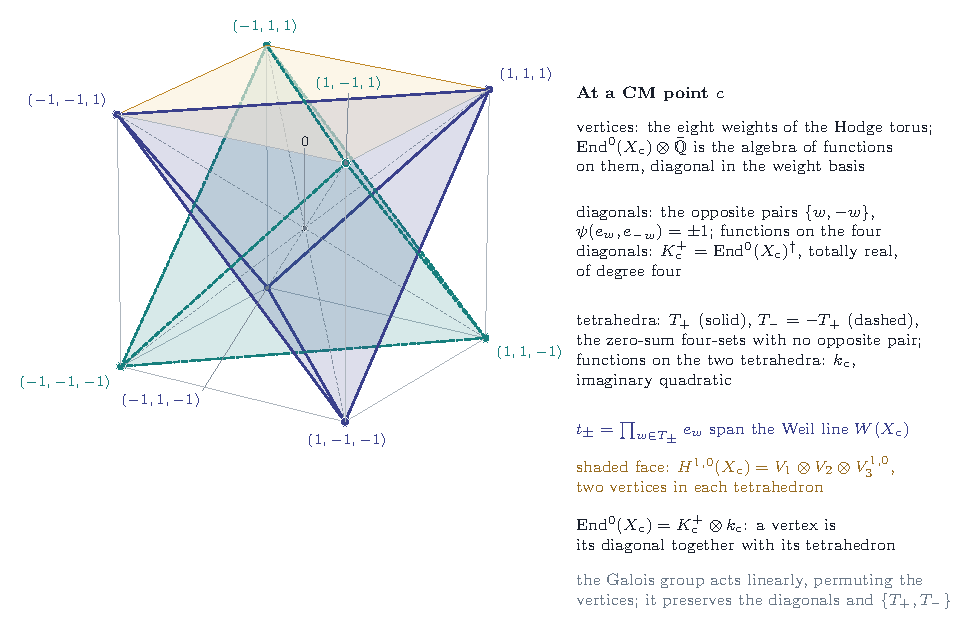
\includegraphics[width=0.96\textwidth]{fig_cmcube}
\caption{\Cref{prop:cmsource}(i). The eight weights $(\pm1,\pm1,\pm1)$ of the
Hodge torus at a CM point are the vertices of a cube. The four diagonals are
the pairs of opposite weights, paired by the polarisation; the two inscribed
tetrahedra $T_{+}$ (an even number of entries $-1$) and $T_{-}=-T_{+}$ are
the only zero-sum four-sets without an opposite pair, and $t_{\pm}=\prod_{w\in
T_{\pm}}e_{w}$ span the Weil line. The Galois group acts by linear maps
permuting the vertices, so it preserves the diagonals and the pair of
tetrahedra: the functions constant on the tetrahedra form the imaginary
quadratic Weil field $k_{c}$, those constant on the diagonals the totally real
quartic algebra $K_{c}^{+}$ of Rosati-fixed endomorphisms, and
$\End^{0}(X_{c})=K_{c}^{+}\otimes k_{c}$ because a vertex is determined by
its diagonal and its tetrahedron.}
\label{fig:cmcube}
\end{figure}

\begin{figure}[tbp]
\centering
  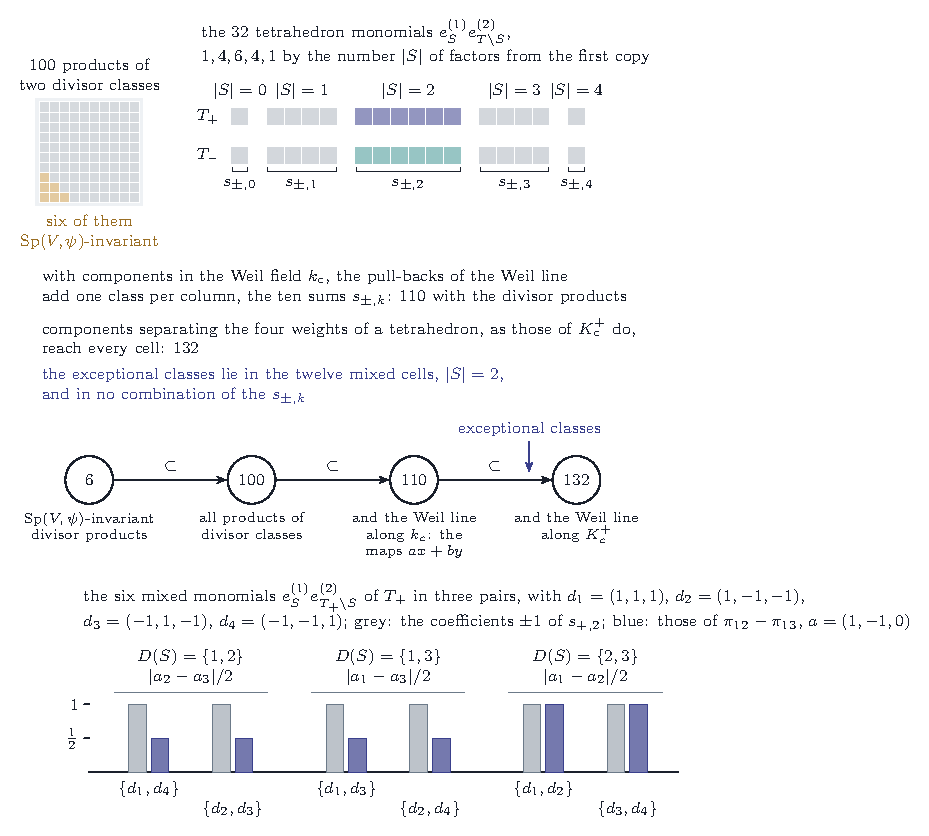
\includegraphics[width=\textwidth]{fig_cmsource}
\caption{\Cref{prop:cmsource}(ii) and (iii). Top: the $132$ Hodge classes of
degree four on the square at a CM point, one cell per monomial of weight
zero. The $100$ products of divisor classes are the cells with an opposite
pair; the $32$ tetrahedron monomials $e^{(1)}_{S}e^{(2)}_{T\setminus S}$ are
arranged by tetrahedron and by the number $|S|$ of factors from the first
copy. Pull-backs of the Weil line along homomorphisms with components in
$k_{c}$ add only the ten symmetric sums $s_{\pm,k}$, one per column, giving
$110$; components separating the four weights of a tetrahedron, as those of
$K_{c}^{+}$ do, separate the monomials and give all $132$. Bottom: on the six
mixed monomials of one tetrahedron, grouped in the three pairs by the
coordinates in which the two weights of $S$ differ, the symmetric sum
$s_{+,2}$ has coefficients $\pm1$ throughout, while an exceptional class
$\omega_{a}$ has coefficients of absolute value $|a_{2}-a_{3}|/2$,
$|a_{1}-a_{3}|/2$, $|a_{1}-a_{2}|/2$, drawn for $\pi_{12}-\pi_{13}$; two
equal absolute values would be a linear relation among the conjugates of an
irrational element of $F$.}
\label{fig:cmsource}
\end{figure}

The CM points fall into two kinds, according to whether the fourfold is
simple; at the points of the second kind the real multiplication comes from
the fixed cubic field $F$.

\begin{lemma}[Split CM points]\label{lem:splitcm}
Let $c\in C$ be a CM point, and let $L\subset D$ be the quadratic extension
of $F$ whose norm one torus $\Res_{F/\QQ}\ker(\Nm_{L/F})$ is the Hodge group
of $X_{c}$ (proof of \Cref{thm:mumfordcm}). Then $L$ is a CM field, and the
following are equivalent: \textup{(a)} $X_{c}$ is not simple; \textup{(b)}
$K_{c}^{+}$ is not a field; \textup{(c)} $L=Fk$ for an imaginary quadratic
field $k\subseteq L$. In that case $k_{c}\cong k$, $K_{c}^{+}\cong\QQ\times F$,
and $X_{c}$ is isogenous to $E\times B$, where $E$ is an elliptic curve with
complex multiplication by $k$ and $B$ is an abelian threefold of CM type on
which the factor $F$ of $K_{c}^{+}$ acts, a real multiplication by $F$; the
Weil line $\HW(X_{c})$ lies in $H^{1}(E)\otimes H^{3}(B)$. At every other CM
point $K_{c}^{+}$ is a totally real quartic field. Points of the second kind
exist for infinitely many $k$: for every imaginary quadratic field $k$ such
that $k\otimes_{\QQ}F_{v}$ is a field at each finite place $v$ of $F$ at
which $D$ is ramified.
\end{lemma}

\begin{proof}
Write $T$ for the Hodge group. By \Cref{prop:cmsource}(i), $\End^{0}(X_{c})
=K_{c}^{+}\otimes k_{c}$ is a product of CM fields on which $\dagger$ is
complex conjugation, and $T$ lies in the centraliser of $\End^{0}(X_{c})$,
which over $\bar{\QQ}$ is the diagonal torus, and in $\Sp(V,\psi)$; so
$T(\RR)$ lies in the compact group of the $x\in(\End^{0}(X_{c})\otimes\RR)
^{\times}$ with $xx^{\dagger}=1$. If $L\otimes_{F,\sigma}\RR$ were
$\RR\times\RR$ at a real place $\sigma$, the factor of $T(\RR)$ at $\sigma$
would be the norm one group of $\RR\times\RR$ over $\RR$, which is not
compact. Hence $L\otimes_{F,\sigma}\RR=\CC$ at each real place, and $L$ is a
CM field.

Over $\bar{\QQ}$, $T=\prod_{\sigma}T_{\sigma}$ with $T_{\sigma}
=\ker(\Nm_{L/F})\otimes_{F,\sigma}\bar{\QQ}$ the diagonal torus of
$\SL_{2}(\bar{\QQ})=(D\otimes_{F,\sigma}\bar{\QQ})^{1}$ for the decomposition
$L\otimes_{F,\sigma}\bar{\QQ}=\bar{\QQ}\times\bar{\QQ}$ by the two embeddings
of $L$ over $\sigma$, one of them chosen and called $\tau_{\sigma}$, the
other $\bar{\tau}_{\sigma}$. The factor $V_{\sigma}$ of
$V=\bigotimes_{\sigma}V_{\sigma}$ (\Cref{setup:mumford}) has the weights
$\tau_{\sigma}$ and $\bar{\tau}_{\sigma}=\tau_{\sigma}^{-1}$ on $T_{\sigma}$,
with eigenvectors $v_{\sigma,\pm}$, and $e_{w}=\bigotimes_{\sigma}
v_{\sigma,w_{\sigma}}$. An element $\gamma$ of the Galois group carries
$V_{\sigma}$ to $V_{\gamma\sigma}$ and $v_{\sigma,+}$ to
$v_{\gamma\sigma,\varepsilon_{\gamma}(\sigma)}$, where
$\varepsilon_{\gamma}(\sigma)=1$ if $\gamma\tau_{\sigma}=\tau_{\gamma\sigma}$
and $-1$ if $\gamma\tau_{\sigma}=\bar{\tau}_{\gamma\sigma}$; so it acts on
the weights by $(\gamma w)_{\gamma\sigma}=\varepsilon_{\gamma}(\sigma)
w_{\sigma}$.

If $L=Fk$, then $\operatorname{Hom}(L,\bar{\QQ})=\operatorname{Hom}(F,\bar{\QQ})
\times\operatorname{Hom}(k,\bar{\QQ})$ with the Galois group acting on both
factors, and with $\tau_{\sigma}=\sigma\otimes\iota_{0}$ for a fixed
embedding $\iota_{0}$ of $k$ the sign $\varepsilon_{\gamma}(\sigma)
=\varepsilon_{\gamma}$ does not depend on $\sigma$: it is $1$ if $\gamma$
fixes $k$ and $-1$ otherwise. Then $\gamma$ permutes the coordinates of a
weight and changes all its signs when it moves $k$. It preserves each
tetrahedron if it fixes $k$ and exchanges the two otherwise, so
$k_{c}\otimes\bar{\QQ}=\bar{\QQ}^{\{T_{+},T_{-}\}}$ is the algebra of the
Galois set $\operatorname{Hom}(k,\bar{\QQ})$, and $k_{c}\cong k$. It carries
the pair $\{\pm(1,1,1)\}$ to itself, so the projection $p_{E}$ onto
$\CC e_{(1,1,1)}\oplus\CC e_{(-1,-1,-1)}$ lies in $\End^{0}(X_{c})$, and by
Poincar\'e reducibility $X_{c}$ is isogenous to $E\times B$ with
$H^{1}(E,\CC)$ the image of $p_{E}$, of dimension two, so $E$ is an
elliptic curve, on whose $H^{1}$ the field $k_{c}$ acts by two conjugate
scalars: $E$ has complex multiplication by $k$. The threefold $B$ has
$\End^{0}(B)\otimes\bar{\QQ}$ containing the diagonal algebra of the six
remaining weights, of dimension $6=2\dim B$, so $B$ is of CM type. Each of
the six remaining weights has exactly one coordinate different from the
other two, and $\gamma$ carries the opposite pair of the weight with
distinguished coordinate $t$ to the pair with distinguished coordinate
$\gamma t$; so the Galois set of the four opposite pairs is the fixed point
$\{\pm(1,1,1)\}$ together with a copy of $\operatorname{Hom}(F,\bar{\QQ})$,
and $K_{c}^{+}\cong\QQ\times F$, the factor $\QQ$ acting on $H^{1}(E)$ and
the factor $F$ on $H^{1}(B)$. Finally $T_{+}$ consists of $(1,1,1)$ and
three weights of $B$, and $T_{-}$ of $(-1,-1,-1)$ and three weights of $B$,
so $t_{\pm}\in H^{1}(E)\otimes H^{3}(B)$ and $\HW(X_{c})$ lies there. This
proves that (c) implies (a) and (b), with the asserted structure.

$X_{c}$ is simple exactly when $\End^{0}(X_{c})=K_{c}^{+}\otimes k_{c}$ is a
field, and since every factor field $E'$ of $K_{c}^{+}$ is totally real,
$E'\otimes k_{c}$ is a field; so (a) and (b) are equivalent. Suppose (b).
Then the Galois group does not act transitively on the four opposite pairs,
whose algebra is $K_{c}^{+}$. It acts transitively on the three
coordinates, as on the embeddings of $F$, so some $\gamma$ permutes them
cyclically. For each coordinate $t$ the four pairs fall into two sets of
two, according to the value of the coordinate $t$ on the representatives in
$T_{+}$, and this assigns the three coordinates bijectively to the three
partitions of the four pairs into two sets of two, compatibly with the
Galois action, which preserves or exchanges $T_{+}$ and $T_{-}$. So the
permutation of the pairs induced by $\gamma$ has order divisible by three,
hence equal to three: it is a cycle of length three and fixes exactly one
pair. The orbits of the Galois group on the pairs are therefore either one
orbit or two, of sizes one and three, and by hypothesis some pair
$\{w,-w\}$ is fixed: $\gamma w=\delta_{\gamma}w$ with
$\delta_{\gamma}=\pm1$ for every $\gamma$. Replace the choice of
$\tau_{\sigma}$ by $\tau'_{\sigma}=\tau_{\sigma}$ if $w_{\sigma}=1$ and
$\tau'_{\sigma}=\bar{\tau}_{\sigma}$ if $w_{\sigma}=-1$; for the new choice
$w$ becomes $(1,1,1)$, and the new signs are
$\varepsilon'_{\gamma}(\sigma)=\varepsilon_{\gamma}(\sigma)w_{\sigma}
w_{\gamma\sigma}=\delta_{\gamma}$ for all $\sigma$. So $\gamma$ carries the
set $\Phi=\{\tau'_{\sigma}\}$ of three embeddings of $L$ to $\Phi$ if
$\delta_{\gamma}=1$ and to $\bar{\Phi}$ if $\delta_{\gamma}=-1$. The map
$\gamma\mapsto\delta_{\gamma}$ is a character of the Galois group; it is
nontrivial, for otherwise $\Phi$ would be a Galois stable set of three of the
six embeddings and $L$ would not be a field; and complex conjugation carries
every embedding $\tau$ of the CM field $L$ to $\bar{\tau}$, hence $\Phi$ to
$\bar{\Phi}$, so the quadratic field $k$ cut out by the character is
imaginary. Let $\iota_{0}$, $\bar{\iota}_{0}$ be the embeddings of $k$, with
$\iota_{0}$ fixed by the kernel of the character. Then $\tau\mapsto(\tau|_{F},
\iota_{0}\text{ if }\tau\in\Phi\text{ and }\bar{\iota}_{0}\text{ otherwise})$
is a Galois equivariant bijection $\operatorname{Hom}(L,\bar{\QQ})\to
\operatorname{Hom}(F,\bar{\QQ})\times\operatorname{Hom}(k,\bar{\QQ})$, so
$L\cong F\otimes_{\QQ}k$, that is, $L=Fk$ for a copy of $k$ in $L$, which is
(c). At a CM point where (c) fails, $K_{c}^{+}$ is therefore a field, quartic
and totally real by \Cref{prop:cmsource}(i).

Existence. Let $k$ be imaginary quadratic. By the theorem of Albert, Brauer,
Hasse and Noether \cite[\S1.5]{PR94}, the CM field $Fk$ splits $D$, and so
embeds in $D$ over $F$, exactly when $Fk\otimes_{F}F_{v}$ is a field at
every place $v$ of $F$ at which $D$ is ramified, a quadratic extension of a
local field splitting the local quaternion division algebra. At the two real
places where $D$ is definite this holds because $k$ is imaginary, and at the
finite ramified places it is the hypothesis. Given the finitely many
residue characteristics $p$ of these places, choose for each a quadratic
extension $k_{p}$ of $\QQ_{p}$ not contained in $F_{v}$ for any $v$ above
$p$: this is possible since the completions $F_{v}$ above $p$ have degrees
over $\QQ_{p}$ adding up to three, so at most one of them contains a
quadratic extension of $\QQ_{p}$, and then exactly one, while $\QQ_{p}$ has
at least three. Infinitely many imaginary quadratic fields $k$ have the
completions $k_{p}$ at these $p$, and for them
$F_{v}\otimes_{\QQ_{p}}k_{p}$ is a field. For such $k$ let
$T_{k}=\Res_{F/\QQ}\ker(\Nm_{Fk/F})\subset G$, a maximal torus with
$T_{k}(\RR)$ compact. A compact subgroup of $G(\RR)$ fixes a point $x$ of the
symmetric space of $G(\RR)$, and the stabiliser of $x$ is the centraliser of
$h_{x}(\mathbb{S})$; so $h_{x}(\mathbb{S})$ centralises $T_{k}(\RR)$, which
is Zariski dense in $T_{k}$, and lies in $T_{k}(\RR)$. The Hodge group of
the fibre $X_{c}$ over the image $c$ of $x$ is the smallest $\QQ$-subgroup
of $G$ containing $h_{x}(U(1))$, so it lies in $T_{k}$; it has rank three
(proof of \Cref{thm:mumfordcm}), so it equals $T_{k}$, and $c$ is a CM
point with $L=Fk$.
\end{proof}

\begin{remark}[What the degree bound has to control]\label{rem:cmsource}
\leavevmode
\begin{enumerate}[label=\textup{(\arabic*)},leftmargin=2.6em,itemsep=3pt]
\item Markman's theorem \cite{Mar25a}, which the proof of
  \Cref{thm:mumfordcm} invokes, produces the cycles on $X_{c}$ through its
  Weil structure for $k_{c}$. \Cref{prop:cmsource} says that this structure
  is blind to the exceptional classes of the square: everything obtained
  from the Weil line and from divisors by pull-back along homomorphisms with
  components in $k_{c}$, in particular along the maps $(x,y)\mapsto ax+by$,
  and by products, spans $110$ of the $132$ Hodge classes and misses every
  exceptional class; and a representation of an exceptional class by
  pull-backs of the Weil line and products of divisors must use
  homomorphisms whose components, with $k_{c}$, generate the whole
  endomorphism algebra. At a CM point the exceptional classes are thus a
  statement about the real multiplication $K_{c}^{+}$, as they are at a
  general point about the real multiplication by $F$
  (\Cref{prop:mumfordrm}).
\item For $\varphi,\psi\in\End(X_{c})$ and a cycle $Z$ of codimension two on
  $X_{c}$, the degree $\int_{Y}f_{\varphi,\psi}^{*}[Z]\cup\theta_{Y}^{6}$
  is, by \eqref{eq:pullbacktet} applied to the monomials of $[Z]$, a
  polynomial of degree four in the eigenvalues $\varphi_{w}$, $\psi_{w}$,
  which are algebraic integers. For cycles of this shape the bound of
  \Cref{cor:mumfordbounded} therefore asks, at infinitely many CM points,
  for endomorphisms with bounded eigenvalues whose components generate
  $\End^{0}(X_{c})$ over $k_{c}$. Only finitely many algebraic integers of
  degree at most eight have bounded conjugates, so the same finitely many
  minimal polynomials would have to occur at infinitely many points. At
  the split points of \Cref{lem:splitcm} the algebra $K_{c}^{+}=\QQ\times F$
  does not depend on the point and the real multiplication is by $F$ on the
  threefold factor; the representation of the proof of \Cref{thm:mumfordcm}
  then uses, besides elements of $F$, the isogeny $X_{c}\to E\times B$, a
  cycle representing the Weil line of $E\times B$ in
  $H^{1}(E)\otimes H^{3}(B)$, and divisor classes, and these three are what
  varies with the point.
\item At a split point the Weil line is a Hodge class in $H^{1}(E)\otimes
  H^{3}(B)$, a correspondence between an elliptic curve with complex
  multiplication by $k$ and a CM threefold with real multiplication by $F$,
  and its algebraicity is again Markman's theorem for the fourfold
  $E\times B$. A construction of that correspondence with a degree bounded
  independently of $k$, together with a bound on the isogeny and on the
  divisor classes, would give the target through \Cref{cor:mumfordbounded}.
  We do not have one.
\end{enumerate}
\end{remark}

\begin{remark}[Routes to the Mumford target]\label{rem:bypassaudit}
We list the routes to the Mumford target that avoid the Lefschetz standard
conjecture, with what is known about each; \Cref{fig:bypass} summarises
them.
\begin{enumerate}[label=\textup{(\arabic*)},leftmargin=2.6em,itemsep=2pt]
\item \emph{Degeneration.} Closed off: the base is compact and the Hodge
  locus is the base (\Cref{cor:nodegeneration}), so no family on which
  $\omega$ stays of Hodge type approaches the boundary, and there is no limit
  mixed Hodge structure to specialise to.
\item \emph{Deformation into a larger Hodge locus}, on which $\omega$ would
  become a product of divisor classes or a Weil class, hence algebraic by a
  known theorem, and could then be carried back. Closed off by
  \Cref{thm:mumfordrigid}(iii), already to first order.
\item \emph{Hochschild deformations}: twisting $D^{b}(Y)$ by a $B$-field or a
  Poisson bivector, as in the gerby and noncommutative deformations used for
  Weil classes. Closed off: an object with $\ch(E)=N\omega$ extends along no
  direction of $HH^{2}(Y)$ except that of the curve
  (\Cref{cor:mumfordsplit}(i)).
\item \emph{Constructions from line bundles}: cones, tensor products, duals,
  pull-backs and push-forwards along homomorphisms, and Fourier--Mukai
  functors whose kernels are built in the same way. Closed off at every point
  of the curve: everything so built has a Chern character invariant under the
  Lefschetz group, and the exceptional classes are not
  (\Cref{thm:lefschetzclosure}).
\item \emph{Twistor and hyperholomorphic deformation}, the mechanism of
  Markman's proof for Weil classes: move a sheaf along twistor lines on which
  its Chern character stays of Hodge type. Closed off on the square: no
  twistor line through a member of the Mumford family keeps $\omega$ of Hodge
  type, and the twistor lines that do keep it of Hodge type carry
  non-algebraic tori and lie in other components of the Hodge locus
  (\Cref{prop:notwistor}).
\item \emph{Specialisation.} The class is algebraic at every CM point
  (\Cref{thm:mumfordcm}), on every power of $X_{c}$ \cite[Theorem~1.3]{Li26};
  this suffices exactly when the degrees are bounded
  (\Cref{cor:mumfordbounded}), and no bound is known. The cycles that
  represent the class at a CM point must use the real multiplication by the
  Rosati-fixed algebra $K_{c}^{+}$, all of it; the Weil structure of the
  fourfold, with which Markman's theorem produces its cycles, reaches $110$
  of the $132$ Hodge classes and none of the exceptional ones
  (\Cref{prop:cmsource}, \Cref{rem:cmsource}).
\item \emph{Reduction modulo $p$.} At every closed point of every reduction
  of the curve the class is a $\QQ_{\ell}$-combination of algebraic cycles
  (\Cref{prop:modp}), by Li's theorem \cite[Theorem~1.1]{Li26}; this
  suffices, with no lifting step, exactly when the Hilbert data of the cycles
  are bounded on a Zariski dense set of closed points of the arithmetic model
  (\Cref{thm:modpdensity}), and no bound is known.
\item \emph{Semiregularity.} Reduced to one dimension count at one CM point
  (\Cref{thm:mumfordnumerical}); an object attaining it has large odd
  self-extensions (\Cref{thm:mumfordprofile}), is not built from line
  bundles (\Cref{prop:mumforddivisor}) and splits only in a constrained way
  (\Cref{cor:mumfordsplit}); no such object is known.
\item \emph{Kuga--Satake.} Reduced to the Kuga--Satake class of one K3 surface
  of Picard number thirteen (\Cref{thm:mumfordks}), which the known cases of
  the Kuga--Satake Hodge conjecture do not reach (\Cref{rem:mumfordks}). Its
  geometric form is the mechanism of van Geemen and Rapagnetta \cite{vGR26},
  pull-back of the dual Beauville--Bogomolov class of a hyperk\"ahler
  manifold: up to multiples of $\pi_{0}$, the exceptional classes are exactly
  such twisted dual forms of the part of $H^{2}$ of the square generated by
  its symplectic class, and a rational map onto a
  symplectic subvariety of some $S_{\mu}^{[n]}$, $n\ge5$, would suffice;
  K3 surfaces and hyperk\"ahler eightfolds cannot serve
  (\Cref{prop:hksquare}, \Cref{rem:hkroute}).
\item \emph{Motivated classes.} Every Hodge class on an abelian variety is
  motivated \cite[Th\'eor\`eme~0.6.2]{And96b}, so $\omega_{t}$ is motivated for
  every $t$; a motivated class is algebraic once the Lefschetz involutions of
  the auxiliary varieties are (\Cref{prop:lefmot}). Along the family the
  auxiliary variety that suffices is $W\times_{C}W$
  (\Cref{thm:lefschetzpropagation}), and its Lefschetz standard conjecture is
  equivalent to the target (\Cref{cor:mumfordequiv}): the route moves the
  problem and does not shorten it.
\end{enumerate}
Five of the ten routes are closed off by theorems. Of the other five, two
work at special points only, the CM points and the closed points of the
reductions modulo $p$, and each suffices exactly when a degree bound holds;
two are reduced to a single object, one Kuga--Satake class or one perfect
complex with $\dim\Ext^{2}=119$ at one CM point; and one is equivalent to the
target. They are not five separate obligations: three of them are the target itself
in other forms and the other two are stronger inputs that imply it, so any
one of them would suffice (\Cref{cor:mumfordone}, \Cref{rem:mumfordneeded}).
\end{remark}

\begin{figure}[tbp]
\centering
  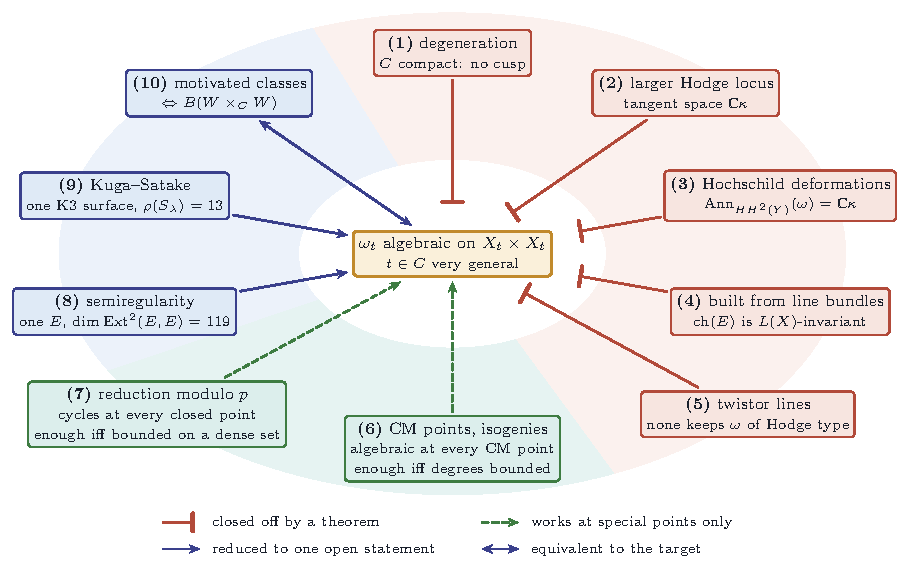
\includegraphics[width=0.96\textwidth]{fig_bypass}
\caption{\Cref{rem:bypassaudit}: the ten routes to the Mumford target that
avoid the Lefschetz standard conjecture. Clay, with a crossed dashed spoke: a
route closed off by a theorem of \Cref{ssec:mumfordrigid} or
\Cref{ssec:mumfordobject}. Grass: a route that works at special points only,
at the CM points or at the closed points of the reductions modulo $p$, and
suffices exactly when a degree bound holds (\Cref{cor:mumfordbounded},
\Cref{thm:modpdensity}). Indigo: a route reduced to one statement, of
the same kind as the target or equivalent to it.}
\label{fig:bypass}
\end{figure}

\subsection{Objects, reduction modulo $p$ and the motivic group}
\label{ssec:mumfordobject}

\Cref{thm:mumfordnumerical} reduces the semiregularity route to one object at
one CM point. We first derive what any object with the right Chern character
must satisfy, whether or not it is semiregular: no sequence of standard
operations produces it from line bundles; it extends along no first order
deformation of $D^{b}(Y)$ other than the direction of the curve; if it is
semiregular, it splits only into summands with no $\Ext^{2}$ between them;
and its self-extensions are large in every degree, with an odd part that the
Euler characteristic forces beyond what Hochschild cohomology supplies. We
then turn to reduction modulo $p$. By Li's proof of the Tate conjecture for
powers of abelian fourfolds over finite fields, the classes are represented
by cycles at every closed point of every reduction of the curve, and the
target is equivalent to a bound on those cycles on a Zariski dense set of
closed points. Finally, the motivic group of $X$ is one of four groups, and
the kinds of algebraic classes known on products of $X$ with other abelian
varieties generate no exceptional class. None of this constructs such an
object or proves the target.

\begin{lemma}[The contraction ranks are symmetric]\label{lem:rankduality}
Let $A$ be an abelian variety of dimension $g$ and $c\in H^{*}(A,\CC)$ a class
each of whose components has Hodge type $(p,p)$ for some $p$. For $k\ge0$ put
$r_{k}(c)=\dim\bigl(HT^{k}(A)\lrcorner\,c\bigr)$, with the action of
\cite[Setup~2.7]{paperII}. Then $r_{k}(c)=r_{g-k}(c)$ for $0\le k\le g$, and
$r_{k}(c)=0$ for $k>g$.
\end{lemma}

\begin{proof}
Write $H^{1,0}=H^{1,0}(A)$ and $A'=H^{0,1}(A)$, both of dimension $g$, so
that $H^{*}(A,\CC)=\bigwedge^{*}H^{1,0}\otimes\bigwedge^{*}A'$ and
$HT^{*}(A)=\bigwedge^{*}(A'\oplus T)$ with $T=(H^{1,0})^{\vee}$. Fix a
generator of $\bigwedge^{g}A'$ and let
$\star\colon\bigwedge^{q}A'\to\bigwedge^{g-q}A'^{\vee}$ send $\eta$ to
$\zeta\mapsto\eta\wedge\zeta$. Under $\Phi=\mathrm{id}\otimes\star$, wedging
with $z\in A'$ becomes, up to a sign fixed on each bigraded piece, contraction
with $z$ on the second factor, while $T$ still contracts the first. So $\Phi$
identifies the action of $HT^{*}(A)$ with the action of
$\bigwedge^{*}U^{\vee}$ by interior products on $\bigwedge^{*}U$, where
$U=H^{1,0}\oplus A'^{\vee}$ has dimension $2g$, up to signs that do not change
ranks. A class of type $(p,p)$ goes to
$\bigwedge^{p}H^{1,0}\otimes\bigwedge^{g-p}A'^{\vee}\subset\bigwedge^{g}U$,
so $\eta=\Phi(c)$ lies in the middle degree whatever the $p$ of its
components. Hence $r_{k}(c)$ is the rank of
$\bigwedge^{k}U^{\vee}\to\bigwedge^{g-k}U$, $x\mapsto\iota_{x}\eta$, which is
zero for $k>g$. Its transpose for the natural pairings is
$\bigwedge^{g-k}U^{\vee}\to\bigwedge^{k}U$, $y\mapsto\pm\iota_{y}\eta$,
because $\langle\iota_{x}\eta,y\rangle=\langle\eta,x\wedge y\rangle
=\pm\langle\iota_{y}\eta,x\rangle$. A map and its transpose have the same
rank.
\end{proof}

\begin{theorem}[The self-extensions of an object with an exceptional Chern
character]\label{thm:mumfordprofile}
Let $c\in C$ and $Y=X_{c}\times X_{c}$, and write
$e_{k}=\dim\Ext^{k}(E,E)$ for a perfect complex $E$ on $Y$.
\begin{enumerate}[label=\textup{(\roman*)},leftmargin=2.6em,itemsep=2pt]
\item For every $E$ and every $k$, $e_{k}\ge r_{k}(\ch E)$ and
  $e_{k}=e_{8-k}$.
\item For a rational exceptional class $\omega=\omega_{a}$ with
  $L_{0}(a)\ne0$: $r_{0}=r_{8}=1$, $r_{1}=r_{7}=16$ and $r_{2}=r_{6}=119$.
\item Let $\omega$ be a rational exceptional class and $\ch(E)=N\omega$
  with $N\ne0$. Then
  \[
    e_{1}+e_{3}=e_{0}+e_{2}+\tfrac12e_{4}
      +\sum_{j\ge1}(-1)^{j}e_{-j}.
  \]
  If $\Ext^{<0}(E,E)=0$, for instance if $E$ is a sheaf, then
  $\sum_{k\ \mathrm{odd}}e_{k}=\sum_{k\ \mathrm{even}}e_{k}$, and
  $e_{1}+e_{3}\ge120+\frac12e_{4}$ when $L_{0}(a)\ne0$.
\end{enumerate}
\end{theorem}

\begin{proof}
(i) The identity $\sigma_{E}\circ\operatorname{ev}_{E}=(\,\cdot\,)\lrcorner
\ch(E)$ of \cite[Setup~2.7]{paperII} holds in every degree, so the kernel of
$\operatorname{ev}_{E}$ on $HT^{k}(Y)$ lies in the annihilator of $\ch(E)$,
and the image of $HT^{k}(Y)$ in $\Ext^{k}(E,E)$ has dimension at least
$r_{k}(\ch E)$. Serre duality with the trivial canonical bundle gives
$e_{k}=e_{8-k}$.

(ii) $r_{0}=1$ because $\omega\ne0$, and $r_{2}=119$ is
\Cref{thm:mumfordrigid}(ii). If $w\in HT^{1}(Y)$ annihilates $\omega$, so does
$w'\wedge w$ for every $w'\in HT^{1}(Y)$, since the annihilator is a left
ideal; for $w\ne0$ these products span a space of dimension $15$, which cannot
lie in $\Ann_{HT^{2}}(\omega)=\CC\kappa$. So $r_{1}=16$, and
\Cref{lem:rankduality} gives $r_{8},r_{7},r_{6}$.

(iii) Since $\ch(E)$ has only a component in $H^{4}$, $\ch(E^{\vee})\ch(E)$
lies in $H^{8}(Y)$ and $\chi(E,E)=\int_{Y}\ch(E^{\vee})\ch(E)=0$, the Todd
class being trivial. By (i) and Serre duality, which also pairs
$\Ext^{-j}$ with $\Ext^{8+j}$,
\[
  0=\chi(E,E)=2(e_{0}-e_{1}+e_{2}-e_{3})+e_{4}
  +2\sum_{j\ge1}(-1)^{j}e_{-j},
\]
which is the displayed identity. With no negative extensions the odd and even
parts are equal, and $e_{0}\ge1$, $e_{2}\ge119$ by (i) and (ii) when
$L_{0}(a)\ne0$.
\end{proof}

\begin{proposition}[Divisor classes do not reach the exceptional classes]
\label{prop:mumforddivisor}
Let $t\in C$ and let $\omega$ be a rational exceptional class. Then $\omega_{t}$
is not in the $\QQ$-span of products of divisor classes of $X_{t}\times
X_{t}$: that span meets the rational Hodge classes of $H^{2}\otimes H^{2}$
exactly in the classes with $\alpha\in\QQ$. Consequently no perfect complex
whose Chern character lies in the subring generated by divisor classes, in
particular no bounded complex of direct sums of line bundles, has
$\ch(E)=N\omega$ with $N\ne0$. At a CM point $c$ the fourfold $X_{c}$ has eight
Hodge classes in $H^{4}$, of which the products of divisor classes span six.
\end{proposition}

\begin{proof}
At a point with Hodge group $G$, the divisor classes of $X_{t}\times X_{t}$ are
the three classes of \Cref{prop:mumfordproduct}(ii), all invariant under
$\Sp(V,\psi)$, and so are their products; the $\Sp(V,\psi)$-invariant part of
$H^{2}\otimes H^{2}$ is spanned by $\pi_{0}$ and $\pi_{12}+\pi_{13}+\pi_{23}$,
the classes with $a_{1}=a_{2}=a_{3}$. At a CM point the Hodge group is a
maximal torus of $G$ (proof of \Cref{thm:mumfordcm}), so the Hodge classes
are the monomials of weight zero. The proof of \Cref{prop:cmsource}(ii)
counts them: $16$ divisor classes $e^{(i)}_{w}e^{(j)}_{-w}$, $132$ Hodge
classes in degree four, of which the products of divisor classes span $100$,
and modulo that span
$\omega_{a}\equiv\frac12\bigl((a_{2}-a_{3})u_{12}+(a_{1}-a_{3})u_{13}
+(a_{1}-a_{2})u_{23}\bigr)$ with $u_{12},u_{13},u_{23}$ linearly independent.
So the span meets that of the four $\pi$ in exactly the classes with
$a_{1}=a_{2}=a_{3}$. For a rational class these
coordinates are the conjugates of $\alpha$, which by \Cref{lem:conjugates} are
equal only if $\alpha\in\QQ$. The Chern character of a complex in the subring
generated by divisor classes has its component in $H^{4}$ in the span of
products of two divisor classes, which excludes $N\omega$. For $X_{c}$ itself
the monomials of weight zero in $H^{4}$ are the six products
$e_{w}e_{-w}e_{w'}e_{-w'}$ over two opposite pairs, which are products of
divisor classes, and the two tetrahedron monomials.
\end{proof}

At a CM point the Hodge classes of $X_{c}$ in $H^{4}$ that are not products
of divisor classes are among the classes that the proof of
\Cref{thm:mumfordcm} pulls back along homomorphisms $X_{c}\times X_{c}\to
X_{c}$; they are algebraic by Markman's theorem \cite{Mar25a}. Li proves,
independently and more generally, that every Hodge class on every power of
every complex CM abelian fourfold is algebraic \cite[Theorem~1.3]{Li26}, which
gives \Cref{thm:mumfordcm} for every power $X_{c}^{n}$ and not only for the
square.

By \Cref{prop:mumforddivisor}, an object with $\ch(E)=N\omega$ cannot have
its Chern character in the subring generated by divisor classes, so it cannot
be assembled from line bundles alone. The next theorem shows that no sequence
of the standard operations of the derived category, applied to line bundles
on powers of $X_{t}$, gets any further.

\begin{theorem}[Objects generated by line bundles]\label{thm:lefschetzclosure}
Let $t\in C$, $X=X_{t}$, and let $L(X)\subseteq\Sp(V,\psi)$ be the Lefschetz
group of $X$, the centraliser of $\End^{0}(X)$ in $\Sp(V,\psi)$. Let
$\mathcal{A}$ be the class of abelian varieties isogenous to a power of $X$;
through an isogeny $X^{n}\to B$ the group $L(X)$ acts diagonally on
$H^{*}(B,\QQ)$, and the action does not depend on the isogeny. Let
$\mathcal{L}$ be the smallest class of objects of the categories
$D^{b}(B)$, $B\in\mathcal{A}$, that contains the line bundles and is closed
under shifts, cones, derived tensor products, derived duals, translations,
the functors $Lf^{*}$ and $Rf_{*}$ for homomorphisms $f$ between members of
$\mathcal{A}$, and the Fourier--Mukai functors $\Phi_{K}\colon D^{b}(B)\to
D^{b}(B')$ with kernel $K\in\mathcal{L}$ on $B\times B'$.
\begin{enumerate}[label=\textup{(\roman*)},leftmargin=2.6em,itemsep=2pt]
\item Every object of $\mathcal{L}$ has an $L(X)$-invariant Chern character.
\item $L(X)=\Sp(V,\psi)$ if $t$ is not a CM point, and $L(X)$ is a maximal
  torus of $\Sp(V,\psi)$ if it is. In both cases the $L(X)$-invariant classes
  on $X\times X$ form the subring generated by divisor classes, of dimensions
  $1,3,6,10,15,10,6,3,1$, respectively $1,16,100,304,454,304,100,16,1$, in
  the degrees $0,2,\dots,16$.
\item No rational exceptional class $\omega_{t}$ is $L(X)$-invariant. Hence
  for no object $E\in\mathcal{L}$ on $X\times X$ and no $N\ne0$ is
  $\ch(E)-N\omega_{t}$ invariant under $L(X)$; in particular
  $\ch(E)\ne N\omega_{t}$.
\item The $\Sp(V,\psi)$-module generated by $\pi_{12}-\pi_{13}$ is
  irreducible, of highest weight $2\varpi_{2}$ and dimension $308$, and it
  meets the span of the four $\pi$ in the plane of the classes with
  $a_{0}=0$ and $a_{1}+a_{2}+a_{3}=0$.
\end{enumerate}
\end{theorem}

\begin{proof}
(i) Two isogenies $X^{n}\to B$ differ by an element of $\End^{0}(X^{n})=
M_{n}(\End^{0}(X))$, which commutes with $L(X)$ acting diagonally, so the
action is well defined. For the same reason a homomorphism $f$ between members
of $\mathcal{A}$ is $L(X)$-equivariant on $H^{1}$, so $f^{*}$ is equivariant
on $H^{*}$, and so is $f_{*}$, which is $f^{*}$ conjugated by Poincar\'e
duality, since $L(X)\subseteq\SL(V)$ fixes the orientation classes.
Translations act trivially on cohomology. The Chern character is additive on
distinguished triangles and multiplicative on derived tensor products,
$\ch(E^{\vee})=\sum_{i}(-1)^{i}\ch_{i}(E)$, $\ch(Lf^{*}E)=f^{*}\ch(E)$, and
$\ch(Rf_{*}E)=f_{*}\ch(E)$ by the Grothendieck--Riemann--Roch theorem
\cite[Theorem~15.2]{Ful98}, the Todd class of an abelian variety being $1$;
and $\Phi_{K}=Rp_{2*}(p_{1}^{*}(\,\cdot\,)\otimes^{L}K)$. So the objects with
$L(X)$-invariant Chern character form a class with all the closure
properties, and it remains to see that it contains the line bundles, that is,
that $c_{1}(\mathcal{O}(D))$ is $L(X)$-invariant. Pulled back along an
isogeny, which is injective on rational cohomology, $c_{1}$ becomes a Hodge
class of degree two on some $X^{n}$, an element of the invariants of the
Hodge group in ${\textstyle\bigwedge^{2}}(V^{\vee}\otimes\QQ^{n})=
{\textstyle\bigwedge^{2}}V^{\vee}\otimes S^{2}\QQ^{n}\oplus S^{2}V^{\vee}
\otimes{\textstyle\bigwedge^{2}}\QQ^{n}$. If $t$ is not a CM point, the Hodge
group is $G$, whose invariants in ${\textstyle\bigwedge^{2}}V$ are the multiples of $\psi$
and in $S^{2}V$ are zero, since every summand of $S^{2}(V_{1}\otimes V_{2}
\otimes V_{3})$ contains a factor $S^{2}V_{i}$; so the Hodge classes of degree
two are $\Sp(V,\psi)$-invariant. If $t$ is a CM point, a monomial of degree two
in a weight basis has weight zero for the Hodge torus exactly when its two
weights are opposite, and then it has weight zero for $L(X)$, by the
description in (ii).

(ii) If $t$ is not a CM point, $\End^{0}(X)=\QQ$ and $L(X)=\Sp(V,\psi)$. At a
CM point $\End^{0}(X)\otimes\CC$ is the algebra of diagonal matrices in a
weight basis (proof of \Cref{thm:mumfordcm}), and $\psi$ pairs each weight
with its opposite only, so $L(X)_{\CC}$ is the torus of diagonal matrices
$\operatorname{diag}(\lambda_{w})$ with $\lambda_{w}\lambda_{-w}=1$, of rank
four. For $t$ not CM, the first fundamental theorem for $\Sp(V,\psi)$
\cite[Chapter~5]{GW09} shows that its invariants in
${\textstyle\bigwedge^{*}}(V\otimes\QQ^{2})$ are spanned by the products of
the three quadratic invariants, which are the divisor classes. Their
dimensions follow from the skew Cauchy formula
${\textstyle\bigwedge^{2m}}(V\otimes\QQ^{2})=\bigoplus_{\lambda}S_{\lambda}V
\otimes S_{\lambda'}\QQ^{2}$, over the partitions $\lambda=(2^{r},1^{s})$ of
$2m$ with at most two columns, and the rule that $S_{\lambda}V$ contains the
trivial representation of $\Sp(V,\psi)$, then once, exactly when both columns
of $\lambda$ have even length at most $8$ \cite{GW09}: the invariants of
degree $2m$ have dimension $\sum(s+1)$, over the even $r,s\ge0$ with
$2r+s=2m$ and $r+s\le8$, which is $1,3,6,10,15,10,6,3,1$ for
$m=0,\dots,8$. At a CM point the invariants are spanned by the
monomials of weight zero for $L(X)$; a set of weights $\pm e_{j}$ with sum
zero is a union of opposite pairs, so each such monomial is, up to sign, a
product of monomials of degree two and weight zero, which are divisor
classes. For each opposite pair $\{w,-w\}$ the four vectors
$e^{(1)}_{\pm w}$, $e^{(2)}_{\pm w}$ give one monomial of weight zero in
degree $0$, four in degree $2$ and one in degree $4$, so the numbers of these
monomials are the coefficients of $(1+4y+y^{2})^{4}$.

(iii) If $t$ is not a CM point, the $\Sp(V,\psi)$-invariant combinations of the
$\pi$ are those with $a_{1}=a_{2}=a_{3}$ (\Cref{prop:mumforddivisor}), and
the coefficients of $\omega_{t}$ are the distinct conjugates of $\alpha$
(\Cref{lem:conjugates}). At a CM point use the map $x\mapsto E_{x}$ of the
proof of \Cref{lem:oneexceptional}, which is $\Sp(V,\psi)$-equivariant: it
carries $\omega_{t}$ to an element $(r,\beta)$ of $\QQ\times F$ with
$\beta\notin\QQ$, acting on $U_{ij}$ by the conjugate $\sigma_{k}(\beta)$
(\Cref{prop:mumfordrm}(ii)), and $\omega_{t}$ is $L(X)$-invariant only if
$E_{\omega_{t}}$ preserves the weight spaces of $L(X)$ in ${\textstyle\bigwedge^{2}}V$. Take
weight vectors $v=x\otimes y\otimes z$ and $w=x\otimes y'\otimes z'$ of
weights $(1,1,1)$ and $(1,-1,-1)$ for the Hodge torus. They are not
opposite, so $v\wedge w$ spans a weight space of $L(X)$, every weight of
$L(X)$ on $V$ having multiplicity one. But
$v\wedge w=(x\cdot x)\otimes\bigl(y\cdot y'\otimes z\wedge z'+y\wedge y'
\otimes z\cdot z'\bigr)$ has nonzero components in $U_{12}$ and in $U_{13}$,
on which $E_{\omega_{t}}$ acts by $\sigma_{3}(\beta)\ne\sigma_{2}(\beta)$. So
the line is not preserved. The rest of (iii) follows from (i).

(iv) Write $H^{2}(X)=\QQ\theta\oplus P$, with $P$ the primitive part, the
irreducible $\Sp(V,\psi)$-module of highest weight $\varpi_{2}$ and dimension
$27$. Through the form ${\textstyle\bigwedge^{2}}\psi$ the four $\pi$ are
self-adjoint endomorphisms of $H^{2}(X)$, and $\pi_{12}-\pi_{13}$ kills
$\theta$ and is a trace-free self-adjoint endomorphism of $P$, an element of
$S^{2}P$ orthogonal to the invariant. Restricting
$S^{2}({\textstyle\bigwedge^{2}}V)=S_{(2,2)}V\oplus{\textstyle\bigwedge^{4}}V$
from $\GL(V)$ to $\Sp(V,\psi)$ gives, with dimensions $336=308+27+1$ and
$70=42+27+1$, the decomposition $S^{2}P=V(2\varpi_{2})\oplus V(\varpi_{4})
\oplus V(\varpi_{2})\oplus\QQ$. The element $\pi_{12}-\pi_{13}$ is
$G$-invariant. The summand $V(\varpi_{2})\cong P$ has no $G$-invariant, since
$({\textstyle\bigwedge^{2}}V)^{G}=\QQ\theta$, and neither has $V(\varpi_{4})$,
which lies in ${\textstyle\bigwedge^{4}}V$, whose $G$-invariants are the line
of $\theta^{2}$ (\Cref{prop:mumfordproduct}(i)), invariant under all of
$\Sp(V,\psi)$. So $\pi_{12}-\pi_{13}$ is a nonzero vector of the irreducible
module $V(2\varpi_{2})$, which it generates; its dimension is $308$ by Weyl's
dimension formula. The same argument puts every trace-free combination of
$\pi_{12},\pi_{13},\pi_{23}$ in $V(2\varpi_{2})$, while $\pi_{0}$ and
$\pi_{12}+\pi_{13}+\pi_{23}$ are $\Sp(V,\psi)$-invariant and independent
modulo it; so adding the four $\pi$ raises the dimension by two.
\end{proof}

\Cref{fig:hodgecount} compares the Hodge classes of $X_{t}\times X_{t}$ with
the subring generated by divisor classes, degree by degree.

\begin{figure}[htbp]
\centering
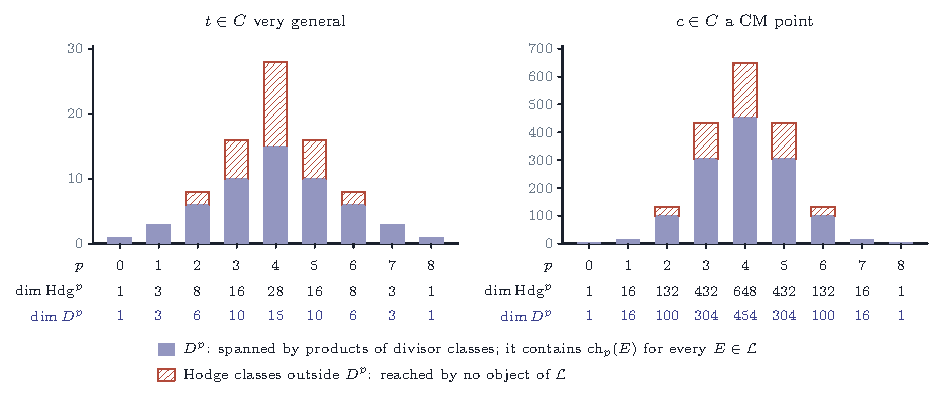
\includegraphics[width=\textwidth]{fig_hodgecount}
\caption{\Cref{thm:lefschetzclosure}(ii). The Hodge classes of
$X_{t}\times X_{t}$ degree by degree, against the subring $D^{p}$ generated
by divisor classes, which contains the Chern character of every object of
$\mathcal{L}$: at a very general point of the Mumford curve (left) and at a
CM point (right). The hatched classes, the exceptional ones among them, are
reached by no object of $\mathcal{L}$.}
\label{fig:hodgecount}
\end{figure}

\begin{remark}[Where a construction has to leave $\mathcal{L}$]
\label{rem:leavel}
\Cref{thm:lefschetzclosure} extends \Cref{prop:mumforddivisor} from sums of
line bundles to everything the standard operations make out of them, at every
point of the curve, including the CM points, where the exceptional classes
are algebraic. There the cycles that represent them are not Chern characters
of objects of $\mathcal{L}$, and neither are the two Hodge classes of $X_{c}$
in degree four that are not products of divisor classes. At a point that is
not CM, every Chern character of an object of $\mathcal{L}$ lies in the
isotypic component of the trivial representation of $\Sp(V,\psi)$, while by
\Cref{thm:lefschetzclosure}(iv) an object with $\ch(E)=N\omega$ must have a
nonzero component in the one of highest weight $2\varpi_{2}$. Every
construction of such an object therefore contains a step that does not commute with the Lefschetz group on
cohomology: passing to a direct summand, a subobject or a Jordan--H\"older
factor, choosing a point of a moduli space, or deforming from a member with
more endomorphisms. The last is what semiregularity does along the curve
(\Cref{thm:mumfordnumerical}).
\end{remark}

\begin{lemma}[The summands of a semiregular object]\label{lem:semiregsum}
Let $Z$ be a smooth projective variety and $E_{1},E_{2}$ perfect complexes on
$Z$. On $\Ext^{2}(E_{1}\oplus E_{2},E_{1}\oplus E_{2})=\bigoplus_{i,j}
\Ext^{2}(E_{j},E_{i})$ the semiregularity map is
$\sigma_{E_{1}\oplus E_{2}}(\zeta)=\sigma_{E_{1}}(\zeta_{11})
+\sigma_{E_{2}}(\zeta_{22})$. So $\sigma_{E_{1}\oplus E_{2}}$ is injective if
and only if $\sigma_{E_{1}}$ and $\sigma_{E_{2}}$ are injective, their images
meet only in zero, and $\Ext^{2}(E_{1},E_{2})=\Ext^{2}(E_{2},E_{1})=0$.
\end{lemma}

\begin{proof}
The Atiyah class is natural, so $\mathrm{At}(E_{1}\oplus E_{2})$ is the
diagonal sum of $\mathrm{At}(E_{1})$ and $\mathrm{At}(E_{2})$. In
$\sigma(\zeta)=\sum_{q}\frac1{q!}\operatorname{tr}(\zeta\circ\mathrm{At}^{q})$
of \cite[Theorem~2.2]{paperII} the composite $\zeta\circ\mathrm{At}^{q}$ has diagonal blocks
$\zeta_{ii}\circ\mathrm{At}(E_{i})^{q}$, and the trace of a block matrix of
morphisms is the sum of the traces of its diagonal blocks. In particular the
off-diagonal blocks $\zeta_{12}$ and $\zeta_{21}$ lie in the kernel, so
injectivity forces them to vanish; on the diagonal blocks the map is
$(\zeta_{11},\zeta_{22})\mapsto\sigma_{E_{1}}(\zeta_{11})+\sigma_{E_{2}}
(\zeta_{22})$, which is injective exactly when both summands are injective
and their images meet only in zero.
\end{proof}

The condition on the images cannot be dropped, and the objects that show it
are the simplest ones: the structure sheaves of abelian subvarieties of half
dimension, each of which is semiregular on its own.

\begin{lemma}[Abelian subvarieties of half dimension are semiregular]
\label{lem:absemireg}
Let $A$ be an abelian variety of dimension $2n$ and $B\subseteq A$ an abelian
subvariety of dimension $n$. Then $\operatorname{ev}_{\cO_{B}}\colon
HT^{2}(A)\to\Ext^{2}(\cO_{B},\cO_{B})$ is surjective, its kernel is
$\Ann_{HT^{2}}([B])$, of dimension $6n^{2}-n$, and $\sigma_{\cO_{B}}$ is
injective.
\end{lemma}

\begin{proof}
The normal bundle of $B$ is trivial, so $\ch(\cO_{B})=[B]$ by the
Grothendieck--Riemann--Roch theorem for the embedding, and
$\Ext^{*}(\cO_{B},\cO_{B})\cong{\textstyle\bigwedge^{*}}\CC^{2n}$ (proof of
\cite[Corollary~3.17]{paperII}), so $\dim\Ext^{2}(\cO_{B},\cO_{B})=\binom{2n}{2}
=2n^{2}-n$, while $\dim HT^{2}(A)=2\binom{2n}{2}+4n^{2}=8n^{2}-2n$. Choose a
complementary abelian subvariety $B'$; the isogeny $B\times B'\to A$
identifies $H^{1}(A,\CC)$ with $H^{1}(B)\oplus H^{1}(B')$ compatibly with the
Hodge decompositions, identifies $HT^{2}(A)$ with $HT^{2}(B\times B')$
compatibly with contraction, and carries $[B]$ to a nonzero multiple of
$1\otimes[\mathrm{pt}_{B'}]$, where $[\mathrm{pt}_{B'}]$ spans
${\textstyle\bigwedge^{2n}}H^{1}(B')$. Write $T=T_{B}\oplus T_{B'}$ for the
tangent space and $H^{0,1}(A)=H^{0,1}(B)\oplus H^{0,1}(B')$. A class
$\zeta\in H^{0,2}(A)={\textstyle\bigwedge^{2}}H^{0,1}(A)$ has
$\zeta\cup[B]=\zeta_{BB}\otimes[\mathrm{pt}_{B'}]$, with $\zeta_{BB}$ its
component in ${\textstyle\bigwedge^{2}}H^{0,1}(B)$, because every factor from
$H^{0,1}(B')$ is killed by the top class of $B'$; so the annihilator in
$H^{0,2}$ has dimension $\binom{2n}{2}-\binom{n}{2}$. For $a\otimes v\in
H^{0,1}(A)\otimes T=H^{1}(T_{A})$ the contraction is $a\wedge(v\lrcorner[B])
=a_{B}\otimes(v_{B'}\lrcorner[\mathrm{pt}_{B'}])$, since $v_{B}$ kills
$[\mathrm{pt}_{B'}]$ and $a_{B'}\wedge(v_{B'}\lrcorner[\mathrm{pt}_{B'}])$
would have type $(n-1,n+1)$ on the $n$-fold $B'$; the map
$v\mapsto v_{B'}\lrcorner[\mathrm{pt}_{B'}]$ has rank $n$, as does
$a\mapsto a_{B}$, so the contraction has rank $n^{2}$ on the space
$H^{0,1}(A)\otimes T$ of dimension $4n^{2}$ and the annihilator there has
dimension $3n^{2}$. For $\vartheta\in{\textstyle\bigwedge^{2}}T$ only the
component in ${\textstyle\bigwedge^{2}}T_{B'}$ contracts $[\mathrm{pt}_{B'}]$
nontrivially, and injectively; so the annihilator in
${\textstyle\bigwedge^{2}}T$ has dimension $\binom{2n}{2}-\binom{n}{2}$.
Altogether $\dim\Ann_{HT^{2}}([B])=2\binom{2n}{2}-2\binom{n}{2}+3n^{2}
=6n^{2}-n$. By the square $\sigma_{E}\circ\operatorname{ev}_{E}=
(\,\cdot\,)\lrcorner\ch(E)$ of \cite[Setup~4.54]{paperII} the kernel of
$\operatorname{ev}_{\cO_{B}}$ lies in $\Ann_{HT^{2}}([B])$, so
$\operatorname{ev}_{\cO_{B}}$ has rank at least $(8n^{2}-2n)-(6n^{2}-n)
=2n^{2}-n=\dim\Ext^{2}(\cO_{B},\cO_{B})$: it is surjective and its kernel is
the annihilator. If $\sigma_{\cO_{B}}(y)=0$, write $y=\operatorname{ev}(x)$;
then $x\lrcorner[B]=0$, so $x$ lies in the annihilator, which is the kernel,
and $y=0$.
\end{proof}

\begin{remark}[Sums of abelian subvarieties]\label{rem:absums}
Let $B_{1},\dots,B_{r}\subseteq A$ be abelian subvarieties of dimension
$n\ge3$, translated so that any two of them meet in finitely many points or
not at all, which generic translates achieve, and let $E=\bigoplus_{j}
\cO_{B_{j}}[k_{j}]$. The sheaves $\mathcal{E}xt^{q}(\cO_{B_{i}},\cO_{B_{j}})$
for $i\ne j$ are supported on $B_{i}\cap B_{j}$ and vanish for $q\ne n$,
by the Koszul resolution of $\cO_{B_{i}}$ restricted to $B_{j}$, so
$\Ext^{2}(\cO_{B_{i}}[k_{i}],\cO_{B_{j}}[k_{j}])=H^{2+k_{j}-k_{i}-n}
(B_{i}\cap B_{j},\mathcal{E}xt^{n})$ vanishes when all $k_{j}$ are equal and
$n\ge3$, and when $|k_{i}-k_{j}|\le1$ and $n\ge4$; and each
$\sigma_{\cO_{B_{j}}}$ is injective by \Cref{lem:absemireg}. In these cases
every hypothesis of \Cref{lem:semiregsum}, applied to one summand and the
sum of the others, holds except the one on the images. Now let $v\in HT^{2}(A)$
satisfy $v\lrcorner\ch(E)=\sum_{j}(-1)^{k_{j}}v\lrcorner[B_{j}]=0$ with
$v\lrcorner[B_{1}]\ne0$. Then $\zeta=\bigoplus_{j}\operatorname{ev}_{\cO_{B_{j}}}(v)$
is nonzero, because $v$ is not in the annihilator of $[B_{1}]$, and
$\sigma_{E}(\zeta)=\sum_{j}(-1)^{k_{j}}v\lrcorner[B_{j}]=0$: the images of
the $\sigma_{\cO_{B_{j}}}$ meet, and $E$ is not semiregular. This is exactly
the situation at a member of a Weil family on which a Weil class is a
combination of classes of abelian subvarieties of dimension $n$, as on a
product of elliptic curves: a tangent direction $v$ of the family keeps
$\ch(E)$ of Hodge type but moves any $[B_{j}]$ outside
$\QQ\theta^{n}\oplus\HW(A)$, and \cite[Corollary~3.17]{paperII} excludes such sums
for this reason. The sum is obstructed although its summands are not.
\end{remark}

\begin{corollary}[Hochschild deformations and direct summands]
\label{cor:mumfordsplit}
Let $c\in C$, $Y=X_{c}\times X_{c}$, $\omega=\omega_{a}$ a rational
exceptional class with $L_{0}(a)\ne0$, and $E$ a perfect complex on $Y$ with
$\ch(E)=N\omega$, $N\ne0$.
\begin{enumerate}[label=\textup{(\roman*)},leftmargin=2.6em,itemsep=2pt]
\item $E$ extends to the first order deformation of $D^{b}(Y)$ given by
  $x\in HH^{2}(Y)=HT^{2}(Y)$ only if $x\in\CC\kappa$. No $B$-field, no
  Poisson bivector and no commutative deformation off the curve carries it.
\item If $\sigma_{E}$ is injective and $E=E_{1}\oplus E_{2}$ with both
  summands nonzero, then $\Ext^{2}(E_{1},E_{2})=\Ext^{2}(E_{2},E_{1})=0$, each
  $\sigma_{E_{i}}$ is injective, each $E_{i}$ extends to first order along the
  curve, and $\kappa\lrcorner\ch(E_{i})=0$. If moreover
  $\dim\Ext^{2}(E,E)=119$, then $\dim\Ext^{2}(E_{i},E_{i})=
  120-\dim\Ann_{HT^{2}}(\ch E_{i})$, and
  \[
    \Ann_{HT^{2}}(\ch E_{1})+\Ann_{HT^{2}}(\ch E_{2})=HT^{2}(Y),\qquad
    \Ann_{HT^{2}}(\ch E_{1})\cap\Ann_{HT^{2}}(\ch E_{2})=\CC\kappa .
  \]
\end{enumerate}
\end{corollary}

\begin{proof}
(i) The kernel of $\operatorname{ev}_{E}$ on $HH^{2}(Y)$ is the space of
deformations of $D^{b}(Y)$ along which $E$ deforms to first order
\cite{Tod09}, \cite[Section~8.3]{Mar25a}. If $\operatorname{ev}_{E}(x)=0$ then
$N\,x\lrcorner\,\omega=\sigma_{E}(\operatorname{ev}_{E}(x))=0$, so
$x\in\CC\kappa$ by \Cref{thm:mumfordrigid}(ii). The three kinds of
deformation named are the three summands of $HT^{2}(Y)$.

(ii) The first two assertions are \Cref{lem:semiregsum}. By
\Cref{thm:mumfordnumerical}(ii), $\operatorname{ev}_{E}(\kappa)=0$, and
$\operatorname{ev}_{E}$ is the diagonal sum of $\operatorname{ev}_{E_{1}}$
and $\operatorname{ev}_{E_{2}}$, so each vanishes at $\kappa$; then
$\kappa\lrcorner\ch(E_{i})=\sigma_{E_{i}}(\operatorname{ev}_{E_{i}}(\kappa))
=0$. Put $e(x)=120-\dim\Ann_{HT^{2}}(x)$, the rank of contraction into $x$.
It is subadditive in $x$, and by \Cref{thm:mumfordprofile}(i)
$\dim\Ext^{2}(E_{i},E_{i})\ge e(\ch E_{i})$. The cross terms vanish, so
\[
  119=\dim\Ext^{2}(E,E)=\sum_{i}\dim\Ext^{2}(E_{i},E_{i})
  \ge e(\ch E_{1})+e(\ch E_{2})\ge e(N\omega)=119,
\]
and every inequality is an equality. Hence
$\dim\Ann(\ch E_{1})+\dim\Ann(\ch E_{2})=121$. The intersection of the two
annihilators lies in $\Ann(N\omega)=\CC\kappa$ and contains $\kappa$, so it is
$\CC\kappa$, and the sum has dimension $120$.
\end{proof}

Part (ii) plays for the Mumford classes the role of \Cref{thm:nosum}: a
semiregular object attaining the bound either does not split, or splits into
two pieces whose annihilators fill $HT^{2}(Y)$ and meet only in the direction
of the curve. The two annihilators are the analogue of the two branches $P$
and $Q$ of \cite[Remark~2.10]{paperII}.

\begin{proposition}[Tate classes at every closed point of every reduction]
\label{prop:modp}
There are a finitely generated subring $R\subset\CC$, a model $W_{R}\to
C_{R}$ of $W\to C$ over $R$, with $C_{R}$ smooth and projective over $R$ with
geometrically connected fibres and $W_{R}$ an abelian scheme, projective over
$C_{R}$, and a finite surjective morphism $C'_{R}\to C_{R}$ from a second curve of the same
kind, with the following properties. Put $Y'=(W_{R}\times_{C_{R}}W_{R})
\times_{C_{R}}C'_{R}$, with projection $\pi'\colon Y'\to C'_{R}$, and let
$\omega$ be a rational exceptional class. For every prime $\ell$ there is a
global section $\omega_{\ell}$ of the lisse sheaf
$R^{4}\pi'_{*}\QQ_{\ell}(2)$ on $C'_{R}[1/\ell]$ whose restriction to
$C'_{R}\otimes_{R}\CC$ is the pull-back of $\omega\otimes1$; write
$\omega_{\ell}(\bar{x})$ for its value at a geometric point over a point $x$.
\begin{enumerate}[label=\textup{(\roman*)},leftmargin=2.6em,itemsep=2pt]
\item At a closed point $x$ of $C'_{R}[1/\ell]$ the residue field
  $\kappa(x)$ is finite, $Y'_{x}$ is the square of an abelian fourfold over
  it, and $\omega_{\ell}(\bar{x})$ is fixed by $\Gal(\bar{\kappa}/\kappa(x))$.
\item At such a point $\omega_{\ell}(\bar{x})$ is a $\QQ_{\ell}$-linear
  combination of classes of algebraic cycles of codimension two on $Y'_{x}$,
  defined over $\kappa(x)$.
\item Let $s$ be a closed point of $\Spec R[1/\ell]$ and $\eta_{s}$ the generic
  point of the reduction $C'_{s}$. Then $\omega_{\ell}(\bar\eta_{s})$ is fixed
  by the Galois group of the function field $\kappa(\eta_{s})$, and it is not
  a $\QQ_{\ell}$-linear combination of products of divisor classes of
  $Y'_{\bar\eta_{s}}$.
\end{enumerate}
Every closed point $x$ of a reduction $C_{s}$ of $C$ is the image of a closed
point $x'$ of $C'_{s}$, and $Y'_{x'}=Y_{x}\otimes_{\kappa(x)}\kappa(x')$; so
(i) and (ii) hold at every closed point of every reduction of $C$, after a
finite extension of its residue field.
\end{proposition}

\begin{proof}
\emph{The models.} The family $W\to C$ is defined over a subfield
$k_{1}\subset\CC$ finitely generated over $\QQ$, say as $W_{1}\to C_{1}$. Let
$K_{1}$ be the function field of $C_{1}$ and fix an embedding over $k_{1}$ of
an algebraic closure $\bar{K}_{1}$ into $\CC$; it sends the geometric generic
point of $C_{1}$ to a point $t\in C$, and $Y_{t}=X_{t}\times X_{t}$ is the base
change of $Y_{\bar{K}_{1}}$. The class $\omega_{t}$ is a Hodge class on an
abelian variety, hence absolutely Hodge, so it comes from an absolutely Hodge
class of $Y_{\bar{K}_{1}}$, and $\Gal(\bar{K}_{1}/K_{1})$ acts on these
through a finite quotient \cite[Theorem~2.11 and Proposition~2.9]{Del82}. Let
$K'\subset\bar{K}_{1}$ be a finite extension of $K_{1}$ on which the action is
trivial, $k'$ the algebraic closure of $k_{1}$ in $K'$, and $C'$ the smooth
projective curve over $k'$ with function field $K'$; it is geometrically
connected over $k'$ and maps finitely onto $C_{1}\otimes_{k_{1}}k'$.
Spreading out $W_{1}\to C_{1}$, $C'$ and this map over a finitely generated
subring of $k'$, and inverting one element of it, gives a normal $R$ and
models with the stated properties.

\emph{The section.} By smooth and proper base change
$R^{4}\pi'_{*}\QQ_{\ell}(2)$ is lisse on $C'_{R}[1/\ell]$. Its stalk at the
geometric generic point $\Spec\bar{K}_{1}$ is $H^{4}(Y_{\bar{K}_{1}},
\QQ_{\ell}(2))=H^{4}(Y_{t},\QQ)\otimes\QQ_{\ell}$, and $\omega_{t}\otimes1$
is the $\ell$-adic component of an absolutely Hodge class, so it is fixed by
$\Gal(\bar{K}_{1}/K')$. The scheme $C'_{R}[1/\ell]$ is normal and integral
with function field $K'$, so $\Gal(\bar{K}_{1}/K')$ maps onto its fundamental
group \cite[Tag~0BQI]{Stacks}, and the vector extends to a global section
$\omega_{\ell}$. On the connected curve $C'_{R}\otimes_{R}\CC$ it agrees with
the pull-back of $\omega\otimes1$, the two being global sections of the same
local system that agree at a point over $t$.

(i) and (ii). A scheme of finite type over $\ZZ$ has finite residue fields at
its closed points. A global section of a lisse sheaf is fixed by the
fundamental group of every point, which is (i); and (ii) is Li's theorem
\cite[Theorem~1.1]{Li26}, with $n=r=2$, for the abelian fourfold that is the
fibre of $W_{R}$ at the image of $x$, base changed to $\kappa(x)$.

(iii) The first assertion holds for the same reason as (i). For the second,
let $\bar\eta$ be a geometric generic point of $C'_{R}$ and $\bar{s}$ a
geometric point over $s$. The morphism $C'_{R}\to\Spec R$ is flat and proper
with geometrically connected and geometrically reduced fibres, so the
specialisation map $\pi_{1}(C'_{\bar\eta})\to\pi_{1}(C'_{\bar{s}})$ is
surjective \cite[Tag~0C0P]{Stacks}, and it is compatible with the actions of
the two groups on the first cohomology of the fibres of $W_{R}$, identified by
cospecialisation. The image of $\pi_{1}(C'_{\bar\eta})$ contains that of
$\pi_{1}(C'_{\CC})$, the closure of the image of the topological fundamental
group of a finite cover of $C$, whose Zariski closure contains
$G_{\QQ_{\ell}}$ because the connected monodromy group of $W\to C$ is $G$
(proof of \Cref{cor:mumfordlefschetz}). So the Zariski closure of the
monodromy of $W_{R}$ over $C'_{\bar{s}}$ contains $G_{\QQ_{\ell}}$. A divisor
class of $Y'_{\bar\eta_{s}}$ is defined over a finite extension of
$\kappa(\eta_{s})$, so it is fixed by an open subgroup of the Galois group,
whose image in $\pi_{1}(C'_{s})$ is open \cite[Tag~0BQI]{Stacks} and meets
$\pi_{1}(C'_{\bar{s}})$ in an open subgroup; the Zariski closure of the image
of an open subgroup has the same identity component, so the class is
$G_{\QQ_{\ell}}$-invariant. The $G$-invariants of ${\textstyle\bigwedge^{2}}(V\oplus V)$ are the
three divisor classes of \Cref{prop:mumfordproduct}(ii), which are
$\Sp(V,\psi)$-invariant, so every product of divisor classes of
$Y'_{\bar\eta_{s}}$ is $\Sp(V,\psi)$-invariant. The class
$\omega_{\ell}(\bar\eta_{s})$ corresponds to $\omega\otimes1$, whose
coefficients $a_{1},a_{2},a_{3}$ are the distinct conjugates of $\alpha$
(\Cref{lem:conjugates}), and the $\Sp(V,\psi)$-invariant classes among the
$\omega_{a}$ are those with $a_{1}=a_{2}=a_{3}$ (\Cref{prop:mumforddivisor}).
The last sentence of the statement holds because $C'_{R}\to C_{R}$ is finite
and surjective.
\end{proof}

At the generic point of each reduction the class is therefore a Tate class
over a global function field that is not a combination of products of divisor
classes, exactly as over $\CC$, while at every closed point it is a
combination of classes of cycles. The next theorem shows that a bound on those
cycles is all that is missing, with no passage through $p$-adic Hodge theory.

\begin{theorem}[The Mumford target is a degree bound in positive
characteristic]\label{thm:modpdensity}
Keep \Cref{prop:modp}, fix a prime $\ell$ and a relatively ample line bundle
on $Y'\to C'_{R}$, and for a finite set $\Phi$ of tuples of Hilbert
polynomials say that $\omega$ is \emph{$\Phi$-represented} at a point $x$ of
$C'_{R}[1/\ell]$ if $\omega_{\ell}(\bar{x})=\sum_{i}q_{i}\operatorname{cl}(Z_{i})$
for some $q_{i}\in\QQ_{\ell}$ and closed subschemes $Z_{i}\subset Y'_{\bar{x}}$
of pure codimension two whose Hilbert polynomials form a tuple in $\Phi$. The
following are equivalent.
\begin{enumerate}[label=\textup{(\alph*)},leftmargin=2.6em,itemsep=2pt]
\item $\omega_{t}$ is algebraic for every $t\in C$.
\item For some finite $\Phi$, the closed points of $C'_{R}[1/\ell]$ at which
  $\omega$ is $\Phi$-represented are Zariski dense in $C'_{R}$.
\item For some finite $\Phi$ and some Zariski dense set $S$ of closed points of
  $\Spec R[1/\ell]$, the class $\omega$ is $\Phi$-represented at infinitely
  many closed points of $C'_{s}$ for every $s\in S$.
\end{enumerate}
For a single closed point $s$ of $\Spec R[1/\ell]$, the class $\omega$ is
$\Phi$-represented at infinitely many closed points of $C'_{s}$, for some
finite $\Phi$, if and only if $\omega_{\ell}(\bar\eta_{s})$ is a
$\QQ_{\ell}$-linear combination of classes of algebraic cycles on
$Y'_{\bar\eta_{s}}$.
\end{theorem}

\begin{proof}
One standard property of the $\ell$-adic cycle class is used beyond those over
a field: if $\mathcal{O}$ is a discrete valuation ring in which $\ell$ is
invertible, $\mathcal{Y}\to\Spec\mathcal{O}$ is smooth and projective, and
$\mathcal{Z}\subset\mathcal{Y}$ is a closed subscheme flat over $\mathcal{O}$,
then the specialisation isomorphism of $\ell$-adic cohomology carries the
cycle class of the geometric generic fibre of $\mathcal{Z}$ to that of its
geometric special fibre \cite[Cycle]{SGA4h}. The specialisation isomorphism
also carries the values of a global section of a lisse sheaf to each other,
by its construction.

\emph{Step 1: the represented loci are closed.} For a tuple
$\underline{P}=(P_{1},\dots,P_{m})$ let $\cH_{\underline{P}}$ be the fibre
product over $C'_{R}[1/\ell]$ of the relative Hilbert schemes
$\Hilb^{P_{i}}(Y'/C'_{R}[1/\ell])$. It is projective over $C'_{R}[1/\ell]$
\cite{Gro61}, so it has finitely many connected components. On a component
$T$, with universal subschemes $\mathcal{Z}_{i}$, put $A(h)=\{q\in
\QQ_{\ell}^{m}:\sum_{i}q_{i}\operatorname{cl}(\mathcal{Z}_{i,\bar{h}})
=\omega_{\ell}(\bar{h})\}$ for $h\in T$. If $h'$ is a specialisation of $h$,
there is a discrete valuation ring mapping to $T$ with generic point to $h$ and
closed point to $h'$ \cite[Tag~054F]{Stacks}, and the property above, applied
to the pull-backs of $Y'$ and of the $\mathcal{Z}_{i}$, gives $A(h)=A(h')$.
Any two points of the connected noetherian scheme $T$ are joined by a chain of
specialisations and generisations, through the generic points of its
irreducible components, so $A$ is constant on $T$, say $A_{T}$. Let
$\Sigma_{\underline{P}}$ be the union of the images in $C'_{R}[1/\ell]$ of the
components $T$ with $A_{T}\ne\emptyset$. It is closed, as a finite union of
images of proper morphisms, and it is the set of points at which $\omega$ is
$\{\underline{P}\}$-represented: at a point $x$ of the image of such a $T$, a
closed point of the fibre of $T$ over $x$ has residue field finite over
$\kappa(x)$ and gives subschemes of $Y'_{\bar{x}}$. Put
$\Sigma_{\Phi}=\bigcup_{\underline{P}\in\Phi}\Sigma_{\underline{P}}$.

\emph{Step 2: (b) implies (a).} $\Sigma_{\Phi}$ is closed and contains a dense
set, so it is $C'_{R}[1/\ell]$ and contains the generic point $\xi$ of
$C'_{R}$, whose residue field is $K'$. So $\omega_{t}\otimes1=
\omega_{\ell}(\bar\xi)=\sum_{i}q_{i}\operatorname{cl}(Z_{i})$ with
$q\in\QQ_{\ell}^{m}$ and subschemes $Z_{i}$ of $Y_{\bar{K}_{1}}$, and so of
$Y_{t}$. The cycle class maps are compatible with the comparison isomorphism
$H^{4}(Y_{t},\QQ)\otimes\QQ_{\ell}\cong H^{4}(Y_{t},\QQ_{\ell})$
\cite[Section~1 and Example~2.1(a)]{Del82}, so the linear system
$\omega_{t}=\sum_{i}q_{i}[Z_{i}]$, which has rational coefficients, is
solvable over $\QQ_{\ell}$, hence over $\QQ$, and $\omega_{t}$ is algebraic.
The $Z_{i}$ are defined over a finite extension of $K'$, so they spread out to
subschemes, flat over a nonempty open subset \cite[Tag~052A]{Stacks}, of the
pull-back of $W\times_{C}W$ to a finite cover of $C$, and by the local
constancy of the cycle class used in the proof of \cite[Theorem~16.4]{paperI},
$\omega$ is algebraic at every point of a nonempty Zariski open subset of $C$,
which is uncountable. \Cref{cor:mumfordequiv} gives (a).

\emph{Step 3: (c) implies (b).} Let $D$ be the set of closed points at which
$\omega$ is $\Phi$-represented and $\bar{D}$ its closure. For $s\in S$ the set
$D\cap C'_{s}$ is infinite, so its closure is the irreducible curve $C'_{s}$,
and $C'_{s}\subseteq\bar{D}$. The points $u$ of $\Spec R[1/\ell]$ over which
the fibre of $\bar{D}$ has dimension at least one form a closed set, by the
upper semicontinuity of the dimension of the fibres of a proper morphism
\cite[Tag~0D4I]{Stacks}; it contains the dense set $S$, so it contains the
generic point. The generic fibre of $\bar{D}$ is then a closed subset of
dimension one of the irreducible curve $C'_{R}\otimes_{R}k'$, so it contains
$\xi$, and $\bar{D}=C'_{R}[1/\ell]$.

\emph{Step 4: (a) implies (c).} By (a) and Step 1, applied over $\bar{K}_{1}$
with the Betti class in place of the $\ell$-adic one, $\omega_{t}$ is the
class of a rational combination of subschemes of $Y_{\bar{K}_{1}}$, defined
over a finite extension $L$ of $K'$. Enlarge $R$ to a finitely generated
subring of the algebraic closure of $k'$ in $L$, let $C''_{R}\to C'_{R}$ be the
normalisation in $L$, and spread the subschemes out over $C''_{R}$; by generic
flatness \cite[Tag~052A]{Stacks} they are flat over a dense open subset $U$ of
$C''_{R}[1/\ell]$, with constant Hilbert polynomials. By Step 1 applied on $U$,
$\omega$ is represented by their fibres at every point of $U$. The image of $U$
in $C'_{R}[1/\ell]$ contains a dense open subset $U'$, every closed point of
$U'$ is the image of a closed point of $U$, and $U'$ meets $C'_{s}$ in a
nonempty open, hence infinite, subset for every $s$ in a dense open subset of
$\Spec R[1/\ell]$.

\emph{The single reduction.} If $\omega$ is $\Phi$-represented at infinitely
many closed points of $C'_{s}$, then $\Sigma_{\Phi}\cap C'_{s}$ is closed and
infinite, so it is $C'_{s}$ and contains $\eta_{s}$. Conversely, cycles at
$\bar\eta_{s}$ are defined over a finite extension of $\kappa(\eta_{s})$, and
spreading them out as in Step 4 over a finite cover of $C'_{s}$ represents
$\omega$, with fixed Hilbert polynomials, at every closed point of a nonempty
open subset of $C'_{s}$.
\end{proof}

\begin{remark}[What is left in positive characteristic]\label{rem:modpremains}
By \Cref{prop:modp}(ii) the class is represented at every closed point of
$C'_{R}[1/\ell]$, so \Cref{thm:modpdensity} turns the Mumford target into a
statement of uniformity alone: the Hilbert data of some representation must
stay in one finite set on a Zariski dense set of closed points, for instance
at infinitely many closed points of infinitely many reductions. The passage
to characteristic zero is then done by the specialisation of cycle classes
along $C'_{R}$, and neither the $p$-adic variational Hodge conjecture nor a
lifting of cycles is needed. Li's theorem gives no bound: where its proof
carries cycles into a prescribed isogeny class, it does so by an isogeny whose
degree it does not control \cite[proof of Theorem~1.2, Step~3]{Li26}.

Nor do the natural representatives at the supersingular points supply the
bound. At a closed point $x$ whose fibre is supersingular, the Frobenius
eigenvalues on $H^{2}(Y'_{\bar{x}},\QQ_{\ell}(1))$ are roots of unity, so by
Tate's theorem \cite{Tat66} this space is spanned by divisor classes, and
$\omega_{\ell}(\bar{x})\in{\textstyle\bigwedge^{4}}H^{1}$ is a combination of
products of two of them. But for a closed point $s$ of $\Spec R[1/\ell]$ and
a finite set of Hilbert polynomials, only finitely many closed points of
$C'_{s}$ carry such a combination $\sum_{i}q_{i}\operatorname{cl}(D_{i})
\operatorname{cl}(D'_{i})$ with effective divisors $D_{i},D'_{i}$ whose
Hilbert polynomials lie in that set: otherwise Step~1 of the proof of
\Cref{thm:modpdensity}, run on relative Hilbert schemes of divisors, would
give one at $\bar\eta_{s}$, against \Cref{prop:modp}(iii). This holds whether
or not the supersingular points are dense. They are dense in $C'_{R}$ when $R$
has dimension one. Indeed, for every prime $p\ge5$ not dividing the
discriminants of $F$ and $D$, which is all but finitely many, the
supersingular points of the reduction at a prime over $p$ of Kisin's integral
model of the Shimura curve, with hyperspecial level at $p$, are its whole
Newton jumping locus and number $(p^{r}-1)(g-1)$ on each component of genus
$g$, $r$ being the local degree of $F$ \cite[Theorem~1.2 and
Corollary~5.17]{SZ11}. For all but finitely many $s$ the curve $C'_{s}$ maps
finitely onto such a component, of genus at least two, so it has at least
$p-1$ supersingular points, while a closed subset of $C'_{R}$ of dimension one
meets all but finitely many of the $C'_{s}$ in boundedly many points.

Within one reduction the bound is equivalent to the class being algebraic at
the generic point of $C'_{s}$ (\Cref{thm:modpdensity}), a Tate class over a
global function field that is not a combination of products of divisor
classes (\Cref{prop:modp}(iii)). This is the codimension two case of the
variational Tate conjecture along $C'_{s}$, which Morrow proves for divisors
in its crystalline form \cite{Mor19}. From one reduction alone, the way back
to characteristic zero would be the $p$-adic variational Hodge conjecture for
$W\times_{C}W$ over the Witt vectors of $\kappa(s)$, with rational rather than
$\ell$-adic coefficients and with the crystalline class of the cycle matching
the de Rham class of $\omega$. Bloch, Esnault and Kerz lift such a class in
$K_{0}\otimes\QQ$ of the special fibre to the formal completion for $p>15$,
the dimension being nine, and the algebraisation of the formal class is the
remaining step of their programme \cite[Theorem~1.3]{BEK14}. The route
therefore runs through the uniform bound or through this conjecture.
\end{remark}

Five of the routes of \Cref{rem:bypassaudit} survive the rigidity theorems:
\emph{specialisation}, \emph{reduction modulo $p$}, \emph{semiregularity},
\emph{Kuga--Satake} and \emph{motivated classes}. The next corollary shows
that they are not five separate obligations.

\begin{corollary}[The five routes reduce to one statement]\label{cor:mumfordone}
Let $W\to C$ be as in \Cref{cor:mumfordlefschetz}, let $\omega$ be a rational
exceptional class, and let the \emph{Mumford target} be the first case of
\textup{(F2)}: the Hodge conjecture for $X_{t}\times X_{t}$ for every $t\in C$.
\begin{enumerate}[label=\textup{(\roman*)},leftmargin=2.6em,itemsep=2pt]
\item Each of the following is equivalent to the Mumford target: $\omega_{t}$ is
  algebraic for uncountably many $t\in C$; $B(W\times_{C}W)$ holds for
  $L_{W\times_{C}W}$; $\omega$ is represented with Hilbert data in one finite
  set at infinitely many points of $C$, for instance at infinitely many CM
  points; $\omega$ is represented with Hilbert data in one finite set on a
  Zariski dense set of closed points of the arithmetic model of
  \Cref{thm:modpdensity}.
\item Each of the following implies the Mumford target: a perfect complex $E$
  at one point of $C$ with $\ch(E)=N\omega$, $N\ne0$, no other component, and
  $\dim\Ext^{2}(E,E)=119$; the algebraicity, for uncountably many $t$, of the
  Kuga--Satake class of the surface $S_{\lambda}$ of \Cref{thm:mumfordks}
  attached to $X_{t}$; a rational map as in \Cref{prop:hksquare}(iv), under
  its hypotheses, from $X_{t}\times X_{t}$ for uncountably many $t$.
\item There is a countable set $\Sigma_{0}\subset C$ containing the CM points
  such that the Mumford target holds as soon as the Hodge conjecture holds for
  $X_{c}\times X_{c}$ at one point $c\notin\Sigma_{0}$.
\end{enumerate}
\end{corollary}

\begin{proof}
(i) The first two are \Cref{cor:mumfordequiv}, with \Cref{lem:oneexceptional}
for one class in place of two, the third is \Cref{cor:mumfordbounded} and the
fourth is \Cref{thm:modpdensity}. (ii) The first is
\Cref{thm:mumfordnumerical}(iii). The second and the third give the Hodge
conjecture for $X_{t}\times X_{t}$ at each of the uncountably many points, by
\Cref{thm:mumfordks}(ii) and \Cref{prop:hksquare}(iv), and then (i) applies.
(iii) In the proof of \Cref{cor:mumfordbounded} the set of points at which
$\omega$ is algebraic is the union of the countably many closed sets
$\Sigma_{\underline{P},\underline{q}}$, each finite or equal to $C$. Let
$\Sigma_{0}$ be the union of the finite ones and of the CM points. If
$\omega_{c}$ is algebraic at a point $c\notin\Sigma_{0}$, then $c$ lies in
some $\Sigma_{\underline{P},\underline{q}}$ that is not finite, which is $C$,
and (i) applies.
\end{proof}

\begin{remark}[Which routes are needed]\label{rem:mumfordneeded}
Of the five routes, specialisation, reduction modulo $p$ and motivated
classes are the Mumford target itself in three other forms, by
\Cref{cor:mumfordone}(i) and, for the motivated classes,
\Cref{cor:mumfordequiv}; semiregularity and Kuga--Satake are stronger inputs
that imply it. So any one route suffices. Each of the three
forms is the whole of the problem, a bound on Hilbert data or a case of
\textup{(L)} that is equivalent to the target, and the two stronger inputs
ask for an object and for a cycle.
\end{remark}

The target can also be read at a single member, through the motivic group of
$X$ rather than through cycles on the family; it then becomes the question of
which of four groups this is.

\begin{proposition}[Four possible motivic groups]\label{prop:mumfordmotivic}
In \Cref{setup:mumford}, let $M$ be the group of the Tannakian category of
homological motives generated by $h(X)$, with the Betti realisation as fibre
functor, let $M^{1}=M\cap\Sp(V,\psi)$, and let $N$ be the normaliser of $G$ in
$\Sp(V,\psi)$. Over $\bar{\QQ}$ identify $V_{1}$, $V_{2}$ and $V_{3}$ with one
plane, carrying $\epsilon_{1}$, $\epsilon_{2}$, $\epsilon_{3}$ to one form, and
let $\zeta\in\Sp(V,\psi)(\bar{\QQ})$ be the cyclic permutation
$v_{1}\otimes v_{2}\otimes v_{3}\mapsto v_{3}\otimes v_{1}\otimes v_{2}$ of
the three factors. It normalises $G$, and other identifications change it by
an element of $G(\bar{\QQ})$; so it acts through $V$ on the Hodge classes of
every power of $X$, independently of the choice.
\begin{enumerate}[label=\textup{(\roman*)},leftmargin=2.6em,itemsep=2pt]
\item $N/G$ is a form of the symmetric group $S_{3}$,
  $M=\mathbb{G}_{m}\cdot M^{1}$, and $M^{1}$ is one of $G$, $G\cdot A_{3}$,
  $N$ and $\Sp(V,\psi)$, where $G\cdot A_{3}$ is the inverse image in $N$ of
  the subgroup of order three of $N/G$. The last three contain $\zeta$.
\item The following are equivalent: $M^{1}=G$; the Hodge conjecture holds for
  $X^{n}$ for every $n\ge1$; the two exceptional classes of $X\times X$ are
  algebraic; some algebraic class on some power of $X$ is not fixed by
  $\zeta$.
\item Let $\mathrm{Det}\in(V^{\otimes4})^{G}\subset H^{4}(X^{4},\QQ)$ be the
  Hodge class of \Cref{rem:mumforddet}, and write $r_{1}$ also for the Hodge
  class $t\in(V^{\otimes4})^{G}$ with $\hat{t}=r_{1}=s_{1}+s_{2}+s_{3}$, in the
  notation of Steps~2 and~3 of the proof of \Cref{thm:mumfordpowers}. Both
  are fixed by $N$ and not by $\Sp(V,\psi)$, and each of them is algebraic if
  and only if $M^{1}\ne\Sp(V,\psi)$. So the algebraicity of either excludes
  the last case only; by this argument it does not give the exceptional
  classes, which are not algebraic when $M^{1}$ is $G\cdot A_{3}$ or $N$.
\item Let $W\to C$ be as in \Cref{cor:mumfordlefschetz}, and suppose that it
  is defined over a number field; this holds for the restriction of the
  universal family of a fine moduli space of polarised abelian fourfolds with
  level structure to the normalisation of one of the Shimura curves of
  \cite{Mum69} in it, and for its pull-backs to finite \'etale covers. Then the
  set $\Sigma_{0}$ constructed in the proof of \Cref{cor:mumfordone}(iii) lies
  in $C(\bar{\QQ})$, and the Mumford target holds as soon as, at one point
  $t\in C(\CC)\setminus C(\bar{\QQ})$, some algebraic cycle on some power of
  $X_{t}$ has a class that is not fixed by $\zeta$.
\end{enumerate}
\end{proposition}

\begin{proof}
\emph{The group.} On an abelian variety homological and numerical
equivalence coincide \cite{Lie68}, so the homological motives generated by
$h(X)$ and the Lefschetz motive form a semisimple abelian category
\cite{Jan92}. The K\"unneth projectors are algebraic \cite[\S2]{Kle68}, so
after the usual change of sign in the commutativity constraint this is a
Tannakian category over $\QQ$, with the Betti realisation as a fibre functor,
faithful by the definition of homological equivalence. Its group $M$ is
reductive, the category being semisimple, and the $M$-invariants in the
realisation of a motive $P$ are the image of $\Hom(\mathbf{1},P)$
\cite[Theorem~2.11]{DM82}; so for all $m$ and $p$ the $M$-invariants of
$H^{2p}(X^{m},\QQ)(p)$ are the classes of algebraic cycles. The group $M$ acts
faithfully on $V\oplus\QQ(1)$ and fixes the polarisation class, so it lies in
$\mathrm{GSp}(V,\psi)$ and acts on $\QQ(1)$ through the multiplier. Through
$\psi$ and the K\"unneth projectors every tensor space of $V\oplus\QQ(1)$ is a
sum of direct summands of spaces $H^{k}(X^{k},\QQ)(j)$ cut out by algebraic
projectors, so the $M$-invariants there are algebraic classes, hence Hodge
classes, fixed by $\MT(X)=\mathbb{G}_{m}\cdot G$; as a reductive group is the
subgroup fixing its invariants in the tensor spaces
\cite[Proposition~3.1]{Del82}, $\MT(X)\subseteq M$ and $G\subseteq M^{1}$. An
element of $M$ with multiplier $\nu$ is a square root of $\nu$ times an
element of $M^{1}$, so $M=\mathbb{G}_{m}\cdot M^{1}$. The homotheties act
trivially on the spaces $H^{2p}(X^{m},\QQ)(p)$, so there the algebraic classes
are the $M^{1}$-invariants, as the Hodge classes are the $G$-invariants.

\emph{The groups between $G$ and $\Sp(V,\psi)$.} Over $\bar{\QQ}$ the Lie
algebra $\mathfrak{sp}(V,\psi)\cong S^{2}V$ is the sum of
$\operatorname{Lie}G=T_{1}\oplus T_{2}\oplus T_{3}$, where $T_{i}\cong
S^{2}V_{i}\otimes{\textstyle\bigwedge^{2}}V_{j}\otimes{\textstyle\bigwedge^{2}}V_{k}$, and of
$S^{2}V_{1}\otimes S^{2}V_{2}\otimes S^{2}V_{3}$, which is an irreducible
representation of $G$ of dimension $27$; so a $G$-stable subspace of
$\mathfrak{sp}(V,\psi)$ containing $\operatorname{Lie}G$ is
$\operatorname{Lie}G$ or $\mathfrak{sp}(V,\psi)$. If $H$ is a closed
subgroup with $G\subseteq H\subseteq\Sp(V,\psi)$, its Lie algebra is such a
subspace. If it is $\operatorname{Lie}G$, then $H^{\circ}=G$, which $H$
normalises, so $H\subseteq N$; if it is $\mathfrak{sp}(V,\psi)$, then
$H^{\circ}=\Sp(V,\psi)$, which is connected, so $H=\Sp(V,\psi)$.

\emph{The normaliser.} Since $V$ is absolutely irreducible, the centraliser of
$G$ in $\Sp(V,\psi)$ is $\{\pm1\}$, which lies in $G$ as the image of
$(-1,1,1)$, and $G(\bar{\QQ})$ maps onto the group of inner automorphisms of
$G_{\bar{\QQ}}$. So $N(\bar{\QQ})/G(\bar{\QQ})$ embeds in the outer
automorphism group of $G_{\bar{\QQ}}$, which permutes the three factors,
$\SL_{2}$ having no outer automorphism. The six permutations of the factors,
after identifications as above, preserve $\psi=\epsilon_{1}\otimes
\epsilon_{2}\otimes\epsilon_{3}$ and normalise $G$, so
$N(\bar{\QQ})/G(\bar{\QQ})\cong S_{3}$. The Galois group acts on it by
conjugation through its action on the three factors, which is transitive, and
the subgroups of $S_{3}$ stable under conjugation by a transitive subgroup are
$1$, $A_{3}$ and $S_{3}$. So the algebraic subgroups of $N$ containing $G$ are
$G$, $G\cdot A_{3}$ and $N$, and with the previous paragraph this proves (i),
$\zeta$ mapping to an element of order three of $N/G$.

(ii) If $M^{1}=G$, then $M=\MT(X)$, and every Hodge class on every power of
$X$ is algebraic. The Hodge conjecture for $X\times X$ includes the
exceptional classes. If these are algebraic, so is every rational exceptional
class $\omega_{a}$ of \Cref{setup:omegaa}, and $\omega_{a}$ is not fixed by
$\zeta$: $\zeta$ permutes the three factors cyclically, so it fixes $\theta$
and carries $U_{ij}=S^{2}V_{i}\otimes S^{2}V_{j}\otimes{\textstyle\bigwedge^{2}}V_{k}$
onto $U_{\zeta(i)\zeta(j)}$; labelling the factors so that $\zeta$ sends the
$i$-th to the $(i+1)$-th, it carries $\pi_{12}$ to $\pi_{23}$, $\pi_{23}$ to
$\pi_{13}$ and $\pi_{13}$ to $\pi_{12}$ and fixes $\pi_{0}$. So it fixes
$\omega_{a}$ only if $a_{1}=a_{2}=a_{3}$, whereas these are the distinct
conjugates of an irrational element of $F$ (\Cref{lem:conjugates}). Finally,
if $M^{1}\ne G$, then $M^{1}$ contains $\zeta$ by (i), and every algebraic
class, being $M^{1}$-invariant, is fixed by $\zeta$.

(iii) The class $\mathrm{Det}$ spans $(S^{4}V)^{G}\otimes
{\textstyle\bigwedge^{4}}\QQ^{4}$, where $(S^{4}V)^{G}$ is a line
(\Cref{rem:mumforddet}). As $N$ normalises $G$, it preserves this line, and it
fixes it, because $N(\bar{\QQ})$ is generated by $G(\bar{\QQ})$ and the
permutations of the factors, which fix Cayley's hyperdeterminant, a
symmetric function of the three factors, and the restriction of
$\mathrm{Det}$ to the diagonal is a nonzero multiple of it
(\Cref{rem:mumforddet}). $\Sp(V,\psi)$
fixes no nonzero element of $S^{4}V$, which would be a nonzero quartic form
constant on the single orbit $V\setminus\{0\}$. The permutations of the
factors conjugate $s_{k}$ into $s_{\sigma(k)}$, so they commute with $r_{1}$,
as does $G$; and $t\mapsto\hat{t}$ is $\Sp(V,\psi)$-equivariant, since the
pairing $\int_{X}v\cup w\cup\theta^{3}$ on $V$ is $G$-invariant and
alternating, hence a multiple of the form $\psi$. So the class $r_{1}$ is
fixed by $N$. On $S^{2}V\subset V\otimes V$ the endomorphism $r_{1}$ acts by
$3$ on $S^{2}V_{1}\otimes S^{2}V_{2}\otimes S^{2}V_{3}$ and by $-1$ on the
$T_{i}$, since $s_{k}$ is $1$ on $S^{2}V_{k}$ and $-1$ on
${\textstyle\bigwedge^{2}}V_{k}$; as $S^{2}V$ is irreducible under
$\Sp(V,\psi)$, the class $r_{1}$ is not $\Sp(V,\psi)$-invariant. If
$M^{1}\ne\Sp(V,\psi)$, then $M^{1}\subseteq N$ by (i), and the two classes are
$M^{1}$-invariant, hence algebraic; if $M^{1}=\Sp(V,\psi)$, they are not. When
$M^{1}$ is $G\cdot A_{3}$ or $N$ it contains $\zeta$, which fixes no
exceptional class.

(iv) A fine moduli space as in the statement is defined over a number field,
and the curve contains infinitely many CM points, which are algebraic, an
abelian variety with complex multiplication being defined over a number
field; so the curve is the Zariski closure of a set of algebraic points and
is defined over $\bar{\QQ}$, and so are its normalisation, the restricted
family and their finite \'etale covers. Now let $W\to C$ be defined over
$\bar{\QQ}$. The moduli map of the family is a finite morphism defined over
$\bar{\QQ}$, so the CM points of $C$, whose images are algebraic, lie in
$C(\bar{\QQ})$. The other points of $\Sigma_{0}$ lie in the finite sets
$\Sigma_{\underline{P},\underline{q}}$ of the proof of
\Cref{cor:mumfordbounded}, images of unions of connected components of fibre
products of relative Hilbert schemes of $W\times_{C}W\to C$. These are base
changes of schemes over $\bar{\QQ}$, and each connected component of the
base change is the base change of a connected component over $\bar{\QQ}$,
which is algebraically closed; so a finite
$\Sigma_{\underline{P},\underline{q}}$ consists of algebraic points. If
$t\notin C(\bar{\QQ})$, then $t\notin\Sigma_{0}$, the Hodge group of $X_{t}$ is
$G$, and (ii) for $X_{t}$ gives the Hodge conjecture for $X_{t}\times X_{t}$;
\Cref{cor:mumfordone}(iii) gives the target.
\end{proof}

The four cases differ already on $X^{4}$ and $X^{6}$
(\Cref{fig:mumfordgroups}). Over $\bar{\QQ}$,
$(V^{\otimes2m})^{G}$ is the tensor product of three copies of the space of
$\SL_{2}$-invariants of $(\bar{\QQ}^{2})^{\otimes2m}$, of dimension $c=2$ for
$m=2$ and $c=5$ for $m=3$, with a basis of non-crossing pairings that $\zeta$
and the transpositions of the factors permute. So the algebraic classes in
the multilinear part $V^{\otimes2m}\subset H^{2m}(X^{2m},\QQ)$ have dimension
$c^{3}$, $(c^{3}+2c)/3$, $(c^{3}+3c^{2}+2c)/6$ and $(2m-1)(2m-3)\cdots1$ when
$M^{1}$ is $G$, $G\cdot A_{3}$, $N$ and $\Sp(V,\psi)$, the last by the first
fundamental theorem for $\Sp(V,\psi)$: $8$, $4$, $4$, $3$ on $X^{4}$ and
$125$, $45$, $35$, $15$ on $X^{6}$. The middle two count the orbits of the
basis under $\langle\zeta\rangle$ and under $S_{3}$: $\zeta$ fixes the $c$
triples of equal pairings and a transposition fixes $c^{2}$ of them. If $M$ were known to be
connected, $M^{1}$ would be connected too, since $-1\in G$ lies in its
identity component; it would then be $G$ or $\Sp(V,\psi)$, and the
algebraicity of $\mathrm{Det}$ alone would give the Hodge conjecture for every
power of $X$. The argument does not decide whether $M$ is connected. It is the
standard use of the motivic group as the stabiliser of the algebraic classes,
and we claim no priority for \Cref{prop:mumfordmotivic}. It proves no new case
of the Hodge conjecture: it says what one new cycle on one power of one member
would have to do.

\begin{figure}[tbp]
\centering
  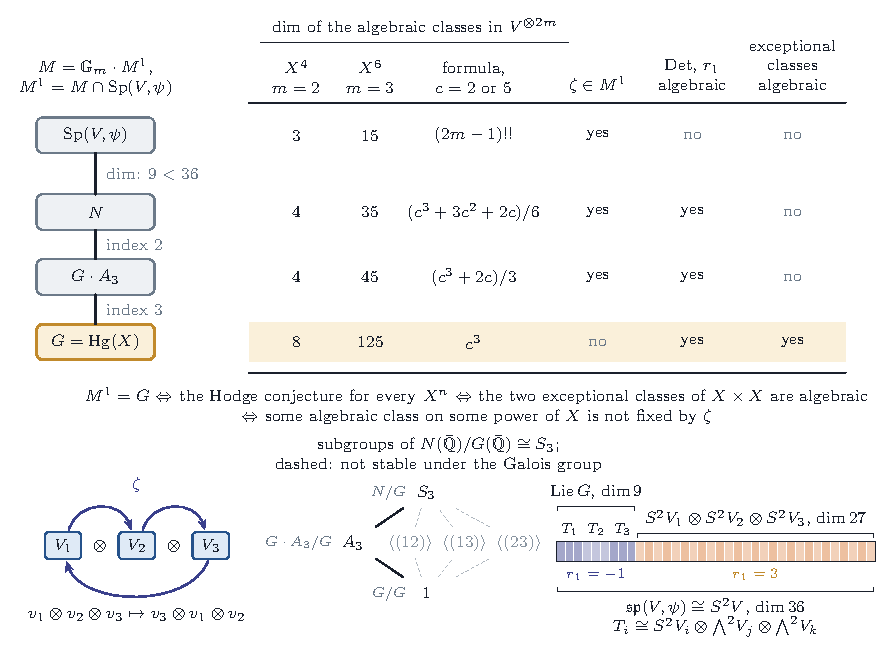
\includegraphics[width=\textwidth]{fig_mumfordgroups}
\caption{The four possible groups $M^{1}=M\cap\Sp(V,\psi)$ of
\Cref{prop:mumfordmotivic}, where $M=\mathbb{G}_{m}\cdot M^{1}$, as the chain
$G\subset G\cdot A_{3}\subset N\subset\Sp(V,\psi)$: the first two inclusions
have index $3$ and $2$, and $N$, whose identity component is $G$, has
dimension $9$ against $36$. For each case the table gives the dimension of
the algebraic classes in the multilinear part $V^{\otimes2m}$ of
$H^{2m}(X^{2m},\QQ)$ for $m=2$ and $m=3$, from the $c=2$, respectively $c=5$,
non-crossing pairings; whether $M^{1}$
contains the cyclic permutation $\zeta$ of the three tensor factors; whether
$\mathrm{Det}$ and $r_{1}$ are algebraic; and whether the two exceptional
classes of $X\times X$ are. Only $M^{1}=G$ makes the exceptional classes
algebraic, and it is equivalent to the Hodge conjecture for every power of
$X$ (\Cref{prop:mumfordmotivic}(ii)); the proposition does not decide which
of the four cases occurs. Below, from left to right: $\zeta$; the subgroups of
$N(\bar{\QQ})/G(\bar{\QQ})\cong S_{3}$, of which only $1$, $A_{3}$ and $S_{3}$
are stable under the Galois group, which acts transitively on the three
factors; and $\mathfrak{sp}(V,\psi)=\operatorname{Lie}G\oplus
S^{2}V_{1}\otimes S^{2}V_{2}\otimes S^{2}V_{3}$, $36=9+27$, the second summand
irreducible under $G$, with the eigenvalues $-1$ and $3$ of $r_{1}$ on the two
summands.}
\label{fig:mumfordgroups}
\end{figure}

The same invariance explains why the classes known or expected to be
algebraic on abelian varieties stop short of the exceptional classes, on all
abelian varieties at once.

\begin{proposition}[The system generated by the known classes]\label{prop:mumfordformal}
Keep \Cref{setup:mumford}, and $\zeta$ and $G\cdot A_{3}$ as in
\Cref{prop:mumfordmotivic}. For an abelian variety $A$ let $A_{X}\subseteq A$
be the largest abelian subvariety isogenous to a power of $X$, and $A'$ the
identity component of the intersection of the kernels of the homomorphisms
$A\to X$. Then $A_{X}\times A'\to A$ is an isogeny, $\Hom(X,A')=0$, and
\[
  H^{1}(A,\QQ)=\bigl(V\otimes\Hom^{0}(A_{X},X)\bigr)\oplus H^{1}(A',\QQ),
\]
the first summand embedded by $v\otimes f\mapsto f^{*}v$. Let $\GL(V)$ act on
$H^{*}(A,\QQ)={\textstyle\bigwedge^{*}}H^{1}(A,\QQ)$ through the factor $V$. Let $\cS$
be the smallest family of subspaces $\cS(A)\subseteq H^{*}(A,\QQ)$, over all
complex abelian varieties $A$, that is closed under linear combinations, cup
products, exterior products, and pull-back and push-forward along
homomorphisms, and contains:
\begin{enumerate}[label=\textup{(\alph*)},leftmargin=2.6em,itemsep=1pt]
\item the divisor classes;
\item for every subfield $E\subseteq\End^{0}(A)$, the rational classes whose
  extension to $\bar{\QQ}$ lies in $\bigoplus_{\sigma}{\textstyle\bigwedge^{d}}
  H^{1}(A,\bar{\QQ})_{\sigma}$, the sum over the embeddings
  $\sigma\colon E\to\bar{\QQ}$ of the top exterior powers of the eigenspaces,
  $d=\dim_{E}H^{1}(A,\QQ)$; among them are the Weil classes;
\item the Hodge classes of the abelian varieties without isogeny factor $X$;
\item the Hodge classes of the powers of $X$ that are fixed by $\zeta$, among
  them $\mathrm{Det}$ and $r_{1}$.
\end{enumerate}
Then every class of $\cS$ is invariant under $G\cdot A_{3}$ acting through
$V$, and the classes obtained from \textup{(a)}, \textup{(b)} and
\textup{(c)} alone are invariant under $\Sp(V,\psi)$. The Hodge classes in
$\cS(X^{m})$ are the Hodge classes of $X^{m}$ fixed by $\zeta$, and $\cS$
contains no exceptional class of $X\times X$.
\end{proposition}

\begin{proof}
Up to isogeny $A=A_{X}\times A'$ by Poincar\'e reducibility, with $A_{X}$
isogenous to some $X^{k}$ and no isogeny factor $X$ in $A'$, so
$\Hom(X,A')=\Hom(A',X)=0$, $X$ being simple. As $\End^{0}(X)=\QQ$,
$\Hom^{0}(A_{X},X)$ has dimension $k$ and the displayed map is an isomorphism.
A homomorphism $h\colon A\to B$ is, up to isogeny, $h_{X}\times h'$ with
$h_{X}\colon A_{X}\to B_{X}$ and $h'\colon A'\to B'$, and $h^{*}$ acts on
$H^{1}$ as $(1\otimes(f\mapsto f\circ h_{X}))\oplus h'^{*}$, which commutes
with $\GL(V)$; so pull-backs are equivariant, and so are cup and exterior
products, $\GL(V)$ acting on $H^{*}(A\times B)=H^{*}(A)\otimes H^{*}(B)$
diagonally. The orientation class of $A$ spans
${\textstyle\bigwedge^{\mathrm{top}}}H^{1}(A)=(\det V)^{\otimes k}\otimes
(\det\Hom^{0}(A_{X},X))^{\otimes8}\otimes{\textstyle\bigwedge^{\mathrm{top}}}H^{1}(A')$, on
which $\SL(V)$ acts trivially, so Poincar\'e duality and push-forwards are
$\SL(V)$-equivariant. Since $G\cdot A_{3}\subseteq\Sp(V,\psi)\subseteq\SL(V)$,
the classes invariant under either group form a family closed under all the
operations, and it remains to look at the generators.

(a) A divisor class of $A$ is the sum of its K\"unneth components in
${\textstyle\bigwedge^{2}}H^{1}(A_{X})$, $H^{1}(A_{X})\otimes H^{1}(A')$ and
${\textstyle\bigwedge^{2}}H^{1}(A')$, which are Hodge classes. The middle one corresponds to a
homomorphism from $A'$ to the dual of $A_{X}$, which is zero. The first is a
Hodge class of $A_{X}$, so a $G$-invariant of ${\textstyle\bigwedge^{2}}(V\otimes\QQ^{k})=
S^{2}V\otimes{\textstyle\bigwedge^{2}}\QQ^{k}\oplus{\textstyle\bigwedge^{2}}V\otimes S^{2}\QQ^{k}$; as
$(S^{2}V)^{G}=0$ and $({\textstyle\bigwedge^{2}}V)^{G}=\QQ\psi$ (proof of
\Cref{thm:lefschetzclosure}(i)), it lies in
$\psi\otimes S^{2}\QQ^{k}$, which $\Sp(V,\psi)$ fixes. On the third $\GL(V)$
acts trivially. (b) The field $E$ acts on $Q=\Hom^{0}(A_{X},X)$ and on
$H^{1}(A')$, and the $\sigma$-eigenspace of $H^{1}(A,\bar{\QQ})$ is
$V\otimes Q_{\sigma}\oplus H^{1}(A',\bar{\QQ})_{\sigma}$. Its top exterior
power is $(\det V)^{\otimes\dim Q_{\sigma}}\otimes(\det Q_{\sigma})^{\otimes8}
\otimes\det H^{1}(A',\bar{\QQ})_{\sigma}$, on which $\SL(V)$ acts trivially.
(c) For such an abelian variety
$A_{X}=0$, and $\GL(V)$ acts trivially. (d) The Hodge classes of $X^{m}$ are
the invariants of $G$, which acts through $V$, and those fixed by $\zeta$ are
invariant under the group $G\cdot A_{3}$ that $G$ and $\zeta$ generate.

So every class of $\cS$ is $G\cdot A_{3}$-invariant, and those obtained from
(a), (b) and (c) are $\Sp(V,\psi)$-invariant. The Hodge classes of $X^{m}$ in
$\cS$ contain those of (d) and are fixed by $\zeta$, so they are exactly the
Hodge classes fixed by $\zeta$; and an exceptional class of $X\times X$ is not
fixed by $\zeta$ (proof of \Cref{prop:mumfordmotivic}(ii)).
\end{proof}

So no argument that uses only these inputs and these operations reaches the
exceptional classes. The inputs include all Weil classes, whether or not they
are known to be algebraic, and with them Markman's cycles \cite{Mar25a}; the
whole Hodge conjecture for the abelian varieties without isogeny factor $X$;
and the algebraicity of $\mathrm{Det}$ and $r_{1}$. A proof needs a cycle
outside this system: on a product of a power of $X$ with an abelian variety, a
class that is not invariant under $G\cdot A_{3}$ acting through $V$, or a cycle
through a variety that is not an abelian variety, such as the Kuga--Satake
class of $S_{\lambda}$ would provide (\Cref{prop:mumfordkslink}).
\Cref{prop:mumfordformal} extends the second limit of
\Cref{rem:mumfordpowersopen}; it is an obstruction to a method, not to the
target, and we claim no priority for it.

The same invariance, used the other way round, shows that the statement (F2)
of \Cref{cor:fourremain} is not smaller than the conjecture for abelian
varieties. For an abelian variety $Y$ let $R(Y)\subseteq H^{*}(Y,\QQ)$ be the
subring generated by divisor classes and Weil classes of quotients, as in
\Cref{rem:f3collapse}.

\begin{proposition}[Statement (F2) is the conjecture for abelian varieties]
\label{prop:f2isab}
Statement \textup{(F2)} of \Cref{cor:fourremain} implies the Hodge
conjecture for every abelian variety, and is therefore equivalent to it.
\end{proposition}

\begin{proof}
The conjecture for abelian varieties contains (F2). For the converse, recall
from \Cref{rem:f3collapse} that (F2) gives every Hodge class of degree $2q$ on
$Y$ as soon as one Hodge class of degree $2q$ on $Y$ lies outside $R(Y)$. Let
$X$ be as in \Cref{setup:mumford}, and let $\zeta$ act on the cohomology of
every abelian variety through the factor $V$, as in \Cref{prop:mumfordformal}.
Every class of $R(Y)$ lies in $\cS(Y)$, so it is fixed by $\zeta$, for every
$Y$; and an exceptional class $e_{0}\in H^{4}(X\times X,\QQ)$ is not
(\Cref{prop:mumfordformal}). Let $\theta$ be an ample class on $X\times X$,
which $\zeta$ fixes. If $\zeta e_{0}=\lambda e_{0}$, then $\lambda\ne1$ and
$e=e_{0}+\theta^{2}$ has $\zeta e=\lambda e_{0}+\theta^{2}$, which is not a
multiple of $e$; otherwise put $e=e_{0}$. In either case $e$ is a Hodge class
of degree $4$ on $X\times X$ with $\zeta e\notin\bar{\QQ}\,e$.

Let $A$ be an abelian variety and $\beta\ne0$ a Hodge class of degree $2p$ on
$A$, and put $Y=A\times X\times X$. As $\zeta$ acts on
$H^{*}(Y)=H^{*}(A)\otimes H^{*}(X\times X)$ diagonally, a class
$\beta\otimes e$ in $R(Y)$ would satisfy
$\zeta\beta\otimes\zeta e=\beta\otimes e$, which forces $\zeta e\in\bar{\QQ}\,e$.
So the Hodge class $\beta\otimes e$ lies outside $R(Y)$, and (F2) makes it
algebraic. In the same way $e\cup\theta^{4}\notin R(X\times X)$, since
otherwise $(\zeta e-e)\cup\theta^{4}=0$ and the hard Lefschetz theorem would
give $\zeta e=e$; so (F2) makes every Hodge class of degree $12$ on
$X\times X$ algebraic. By the Hodge--Riemann bilinear relations the
intersection pairing between the Hodge classes of degrees $4$ and $12$ on
$X\times X$ is nondegenerate, so there is a Hodge class $e'$ of degree $12$
with $\int_{X\times X}e\cup e'=1$. Then
\[
  \beta=\mathrm{pr}_{A*}\bigl((\beta\otimes e)\cup
  \mathrm{pr}_{X\times X}^{*}e'\bigr),
\]
with $\mathrm{pr}_{A}$ and $\mathrm{pr}_{X\times X}$ the projections of $Y$,
and $\beta$ is algebraic.
\end{proof}

\begin{remark}[The rule set with \Cref{prop:f2isab}]\label{rem:f2rule}
\Cref{thm:closure} is a statement about the rule set of \Cref{setup:rules},
and \Cref{prop:f2isab} is a rule that the set does not contain. Adjoined to
it, the rule changes the fifth minimal set of \Cref{thm:closure}(ii): the
minimal sufficient sets become
\[
  \{\mathrm{F3}\},\quad\{\mathrm{L},\mathrm{M}\},\quad
  \{\mathrm{L},\mathrm{F3}'\},\quad\{\mathrm{V},\mathrm{F3}'\},\quad
  \{\mathrm{F2},\mathrm{F3}'\},
\]
and $\mathrm{P2}_{\mathrm{split}}$ lies in none of them. Indeed the new rule
has the premise (F2) and the conclusion $\mathbf{AB}$, the conjecture for
abelian varieties, so the sets $C_{1}$, $C_{2}$ and $C_{4}$ of the proof of
\Cref{thm:closure} stay closed, and a sufficient set meets $H_{1}$, $H_{2}$
and $H_{4}$. The sets meeting these three that are minimal with this property
are the five above, by the argument of that proof without $H_{3}$, and each is
sufficient: $\{\mathrm{F2},\mathrm{F3}'\}$ gives $\mathbf{AB}$ by the new
rule and then $\mathbf{HC}$ by \Cref{prop:f3prime}(i). So the results of this
paper on Weil classes do not shorten a route to the conjecture. What they do
is reduce one case of it, the algebraicity of the Weil classes of every CM
field, to the single statement $\mathrm{P2}_{\mathrm{split}}$, by a route that
does not pass through (F2). Like (F3), which is the whole conjecture, (F2) is
the whole conjecture for abelian varieties, carried by the classes that are
hardest to reach; the exceptional classes of $X\times X$ are its smallest
instance, and the proof above shows that the classes $\beta\otimes e$ built
from them already carry all of it.
\end{remark}

\section{The main theorem in every family}\label{sec:families}

\cite[Theorem~1.1]{paperI} describes the algebraic locus of the Weil classes in one
family: it contains an explicit CM point, it is dense, it is a countable union
of closed algebraic strata, and it is the whole family as soon as it has an
interior point. The first two properties use the Weil classes; the last two
hold for every flat class on every smooth projective family
(\Cref{lem:algstrata}). This section carries the theorem to the families that
carry (F2) and
\textup{(F3$'$)}, and records what each construction of the paper
contributes there.

For (F2) the families are abelian schemes with a member of CM type. Every
Hodge class of every abelian variety lies in such a family
(\Cref{prop:cmfamily}), and (F2) is equivalent to the statement that in every
one of them the algebraic locus of a flat Hodge class that is algebraic at a
CM member has an interior point (\Cref{thm:f2propagation}). The base points
of \cite[Theorem~17.5]{paperI} are the CM seeds of the Weil families, and
Andr\'e's theorem makes the Weil classes of the split families seeds for every
Hodge class of CM type. For \textup{(F3$'$)} the cohomology of a variety splits
into the part reached from abelian varieties by algebraic correspondences and
a complement, and \textup{(F3$'$)} is the statement that the complement
carries no Hodge class (\Cref{prop:abpart}). On the first varieties where
\textup{(F3$'$)} is open, the squares of K3 surfaces with real
multiplication, the algebraic locus of the real multiplication contains every
CM point, is dense and stable under a group of rational Hodge isometries, and
is either everything or meagre (\Cref{thm:rmlocus}). In both cases what is
left is the interior point, and \Cref{thm:twostand} lists what the
constructions of the paper give towards it.

\subsection{Algebraic loci}\label{ssec:algloci}

\begin{definition}[Algebraic locus]\label{def:algloc}
Let $S$ be a smooth connected complex quasi-projective variety,
$f\colon\cX\to S$ a smooth projective morphism, and $\xi$ a global section of
$R^{2p}f_{*}\QQ$ over $S^{\mathrm{an}}$.\footnote{By Ehresmann's theorem $f$
is a locally trivial fibration of differentiable manifolds, so
$R^{2p}f_{*}\QQ$ is a local system with fibre $H^{2p}(\cX_{s},\QQ)$ at $s$. A
global section is a class $\xi_{s}$ on every fibre that is locally constant
under the identifications of nearby fibres, equivalently a class on one fibre
fixed by the monodromy. The set of points $s$ at which $\xi_{s}$ is of type
$(p,p)$ is in general a proper subset of $S$, and it is algebraic by
\cite[Theorem~B.6]{paperI}.} The \emph{algebraic locus} of $\xi$
is
\[
  \Sigma(\xi)=\{\,s\in S:\ \xi_{s}\ \text{is the class of an algebraic cycle
  with rational coefficients on}\ \cX_{s}\,\}.
\]
\end{definition}

\begin{lemma}[The dichotomy in every family]\label{lem:algstrata}
In \Cref{def:algloc} the following hold.
\begin{enumerate}[label=\textup{(\roman*)},leftmargin=2.6em,itemsep=2pt]
\item $\Sigma(\xi)$ is the union of countably many Zariski closed subsets of
  $S$.
\item Either $\Sigma(\xi)=S$, or $\Sigma(\xi)$ is meagre in $S^{\mathrm{an}}$.
\item The following are equivalent: $\Sigma(\xi)=S$; $\Sigma(\xi)$ has an
  interior point; $\Sigma(\xi)$ is not meagre; $\xi_{s}$ is algebraic for
  every $s$ outside a countable union of proper closed analytic subsets of
  $S$. If $\Sigma(\xi)$ is dense, they are also equivalent to $\Sigma(\xi)$
  being closed.
\end{enumerate}
\end{lemma}

\begin{proof}
(i) The proof of \cite[Theorem~16.4]{paperI} applies with
$(\cA,\cS,\omega)$ replaced by $(\cX,S,\xi)$, as in \Cref{lem:spreading}:
for a tuple $\underline{P}$ of Hilbert polynomials the fibre product of the
relative Hilbert schemes $\Hilb^{P_{i}}(\cX/S)$ is projective over $S$
\cite{Gro61}, the class of a flat family of cycles is a flat section, two flat
sections over a connected base that agree at one point agree everywhere, and
the image of a proper morphism is closed. So the set of points at which
$\xi_{s}=\sum_{i}q_{i}[Z_{i}]$ with $Z_{i}$ of Hilbert polynomial $P_{i}$ is
Zariski closed, and $\Sigma(\xi)$ is the union of these strata over the
countably many pairs $(\underline{P},\underline{q})$.

(ii) and (iii). A Zariski closed subset of the irreducible variety $S$ that
has an interior point in $S^{\mathrm{an}}$ is all of $S$, and a proper one is
nowhere dense. If no stratum is $S$, then $\Sigma(\xi)$ is a countable union
of nowhere dense closed sets, hence meagre, and has no interior point, since
$S^{\mathrm{an}}$ is a Baire space. If one stratum is $S$, then
$\Sigma(\xi)=S$. This gives (ii) and the equivalence of the first three
conditions of (iii). The complement of a countable union of proper closed
analytic subsets is not meagre, by the Baire category theorem, so the fourth
condition implies the third, and it is implied by the first. Finally, a
dense set that is closed is $S$.
\end{proof}

So the dichotomy of \cite[Theorem~1.1(iii)]{paperI} and the equivalences of
\cite[Theorem~1.1(iv)]{paperI} hold for every flat class on every smooth projective
family; what \cite[Theorem~1.1]{paperI} adds for the Weil classes is a point of
$\Sigma(\xi)$ and the density, and neither is automatic, since
$\Sigma(\xi)$ may be empty.

\subsection{(F2) is propagation from CM points}\label{ssec:f2cm}

\begin{lemma}[Points of CM type are dense]\label{lem:cmdense}
Let $G$ be a connected reductive group over $\QQ$, let
$u_{0}\colon\mathrm{U}(1)\to G_{\RR}$ be a homomorphism, and let $\cD$ be
the orbit of $u_{0}$ under conjugation by $G(\RR)^{+}$, with the topology of
$G(\RR)^{+}/\mathrm{Stab}(u_{0})$. Then the points $u\in\cD$ for which
$u(\mathrm{U}(1))\subseteq T_{\RR}$ for some maximal torus $T$ of $G$ defined
over $\QQ$ are dense in $\cD$.
\end{lemma}

\begin{proof}
Let $u_{1}\in\cD$ and let $W$ be a neighbourhood of $u_{1}$. The centraliser
of the torus $u_{1}(\mathrm{U}(1))$ in $G_{\RR}$ is connected and reductive,
and a maximal torus of it defined over $\RR$ is a maximal torus $T_{1}$ of
$G_{\RR}$ containing $u_{1}(\mathrm{U}(1))$. Write $\mathfrak{g}$ for the Lie
algebra of $G$ and $\mathfrak{t}_{1}\subseteq\mathfrak{g}_{\RR}$ for that of
$T_{1}$, and choose a regular element $Y_{1}\in\mathfrak{t}_{1}$. The map
$\varphi\colon G(\RR)^{+}\times\mathfrak{t}_{1}\to\mathfrak{g}_{\RR}$,
$(g,Y)\mapsto\mathrm{Ad}(g)Y$, has differential
$(Z,Y')\mapsto[Z,Y_{1}]+Y'$ at $(1,Y_{1})$, which is onto because
$\mathfrak{g}_{\RR}=\mathfrak{t}_{1}\oplus[\mathfrak{g}_{\RR},Y_{1}]$ for a
regular semisimple $Y_{1}$. So for neighbourhoods $N_{1}$ of $1$ in
$G(\RR)^{+}$ with $N_{1}u_{1}N_{1}^{-1}\subseteq W$, and $N_{2}$ of $Y_{1}$
in $\mathfrak{t}_{1}$ consisting of regular elements, the image
$\varphi(N_{1}\times N_{2})$ contains a nonempty open subset of
$\mathfrak{g}_{\RR}$. The rational points $\mathfrak{g}(\QQ)$ are dense in
$\mathfrak{g}_{\RR}$, so that open subset contains some
$Y\in\mathfrak{g}(\QQ)$, and $Y=\mathrm{Ad}(g)Y'$ with $g\in N_{1}$ and
$Y'\in N_{2}$. As $Y$ is rational and regular semisimple, the identity
component $T$ of its centraliser in $G$ is a maximal torus defined over
$\QQ$, and $T_{\RR}=gT_{1}g^{-1}$ because the centraliser of $Y'$ has
identity component $T_{1}$. Then $u=gu_{1}g^{-1}$ lies in $W$ and
$u(\mathrm{U}(1))\subseteq T_{\RR}$.
\end{proof}

For an abelian variety the lemma is used with $G$ its Hodge group, the
smallest algebraic $\QQ$-subgroup of $\GL(H^{1}(A,\QQ))$ whose real points
contain the image of the homomorphism $\mathrm{U}(1)\to\GL(H^{1}(A,\RR))$
that defines the Hodge structure. If $\Hg(A)$ lies in a $\QQ$-torus $T$, then
$A$ is of CM type.\footnote{For an elliptic curve $G=\SL_{2}$ and $\cD$ is
the upper half-plane. The compact torus $u_{\tau}(\mathrm{U}(1))$ fixing
$\tau$ lies in the real points of a maximal $\QQ$-torus of $\SL_{2}$ exactly
when $\tau$ is imaginary quadratic, and the torus is then the group of
elements of norm one of $\QQ(\tau)$. So the points of \Cref{lem:cmdense}
are the curves with complex multiplication, and the lemma is the familiar
density of the imaginary quadratic points in the upper half-plane.} Indeed $T$ lies in a maximal $\QQ$-torus $T'$ of
$\GL(H^{1}(A,\QQ))$, which is the group of units of a commutative semisimple
$\QQ$-subalgebra $L\subseteq\End(H^{1}(A,\QQ))$ of dimension $2\dim A$; the
algebra $L$ commutes with $T'\supseteq\Hg(A)$, so it lies in the commutant of
$\Hg(A)$, which is $\End^{0}(A)$.

\begin{proposition}[A family with a CM member through every Hodge
class]\label{prop:cmfamily}
Let $A_{0}$ be a complex abelian variety and $\gamma$ a Hodge class of degree
$2p$ on $A_{0}$. There are a smooth connected complex quasi-projective variety
$S$, a polarised abelian scheme $\pi\colon\cA\to S$, a global section $\xi$ of
$R^{2p}\pi_{*}\QQ$ that is a Hodge class at every point, and points $s_{0}$,
$c\in S$, such that $\cA_{s_{0}}\cong A_{0}$ with $\xi_{s_{0}}=\gamma$ under
this isomorphism and $\cA_{c}$ is of CM type.
\end{proposition}

\begin{proof}
Let $\ell\ge1$ be an integer with $\ell\gamma$ integral. We construct a
section with value $\ell\gamma$ at $s_{0}$ and divide it by $\ell$ at the
end; until then $\gamma$ stands for $\ell\gamma$. Fix a polarisation of
$A_{0}$, put $V=H_{1}(A_{0},\QQ)$, and fix a level $N\ge3$. As in \cite[Setup~16.1]{paperI}, the
quotient $\cS_{g}$ of the Siegel space $\cH$ of complex structures on
$V_{\RR}$ compatible with the polarisation, by the principal congruence
subgroup of level $N$ of the stabiliser of $H_{1}(A_{0},\ZZ)$, is a smooth
quasi-projective variety carrying a universal family $f\colon\cA_{g}\to\cS_{g}$,
polarised by the fixed polarisation \cite{BB66}; let $a_{0}\in\cS_{g}$ be the
point of $A_{0}$ and $J_{0}\in\cH$ a lift, through which the fibre of
$R^{2p}f_{*}\ZZ$ at every point of the image of $\cH$ is identified with
$H^{2p}(A_{0},\ZZ)=\bigwedge^{2p}H_{1}(A_{0},\ZZ)^{\vee}$ by parallel
transport in the simply connected space $\cH$. Put
$\mathbb{V}=R^{2p}f_{*}\ZZ$, a polarised variation of $\ZZ$-Hodge
structure. By \cite[Theorem~B.6]{paperI} the connected component $\mathcal{C}$ of its
locus of Hodge classes that contains $(a_{0},\gamma)$ is a closed algebraic
subvariety of the total space of $\mathbb{V}$; it has finitely many
irreducible components.

Let $G=\Hg(A_{0})$, which lies in the symplectic group of the polarisation
and fixes $\gamma$ \cite[\S3]{Del82}, let
$u_{0}\colon\mathrm{U}(1)\to G_{\RR}$,
$u_{0}(e^{i\theta})=\cos\theta+J_{0}\sin\theta$, be the homomorphism defining
the Hodge structure, and let
$\cD=\{gJ_{0}g^{-1}:g\in G(\RR)^{+}\}$. For $g\in G(\RR)^{+}$ the complex
structure $J=gJ_{0}g^{-1}$ is compatible with the polarisation and positive
for it, since $g$ preserves the polarisation, so $\cD\subseteq\cH$; and
$\cD$ is the orbit of \Cref{lem:cmdense} when $J$ is identified with
$u_{J}=gu_{0}g^{-1}$. For $J\in\cD$ the group $u_{J}(\mathrm{U}(1))$ lies in
$G(\RR)$, so $\Hg(A_{J})\subseteq G$ fixes $\gamma$, which is therefore a
Hodge class on $A_{J}$. The map sending $J\in\cD$ to the image of $J$ in
$\cS_{g}$ together with $\gamma$ is thus a continuous map from the
connected space $\cD$ to the locus of Hodge classes of $\mathbb{V}$, so it
takes values in $\mathcal{C}$. By \Cref{lem:cmdense} there are points
$J_{k}\in\cD$ converging to $J_{0}$ with $u_{J_{k}}(\mathrm{U}(1))$ in the
real points of a $\QQ$-torus of $G$; then $\Hg(A_{J_{k}})$ lies in that torus
and $A_{J_{k}}$ is of CM type. One of the finitely many irreducible
components of $\mathcal{C}$, say $\mathcal{C}_{0}$, contains the images of
infinitely many $J_{k}$, and, being closed, also their limit $(a_{0},\gamma)$.

Let $\rho\colon S\to\mathcal{C}_{0}$ be a resolution of singularities
\cite{Hir64}: $S$ is smooth, connected and quasi-projective, since
$\mathcal{C}_{0}$ is irreducible and quasi-projective, and $\rho$ is
projective and surjective. Let $\pi\colon\cA\to S$ be the pull-back of
$\cA_{g}$ along $S\to\mathcal{C}_{0}\to\cS_{g}$, a polarised abelian scheme.
A point of $\mathcal{C}_{0}$ is a pair $(a,v)$ with $v\in\mathbb{V}_{a}$ of
Hodge type, and $(a,v)\mapsto v$ is a flat section of the pull-back of
$\mathbb{V}$ to $\mathcal{C}_{0}$, because the total space of a local system
is a covering space of the base; its pull-back to $S$, divided by $\ell$, is
a flat section $\xi$ of $R^{2p}\pi_{*}\QQ$ of Hodge type at every point.
Take $s_{0}$ over $(a_{0},\gamma)$ and $c$ over the image of some $J_{k}$ in
$\mathcal{C}_{0}$.
\end{proof}

\begin{theorem}[(F2) is propagation from CM points]\label{thm:f2propagation}
The following are equivalent.
\begin{enumerate}[label=\textup{(\roman*)},leftmargin=2.6em,itemsep=2pt]
\item \textup{(F2)}.
\item The Hodge conjecture holds for every complex abelian variety.
\item For every polarised abelian scheme $\pi\colon\cA\to S$ over a smooth
  connected complex quasi-projective variety and every global section $\xi$
  of $R^{2p}\pi_{*}\QQ$, if $\xi_{s}$ is algebraic at one point $s\in S$,
  then $\Sigma(\xi)=S$.
\item The same, for the points $s$ at which $\cA_{s}$ is of CM type: if
  $\xi_{c}$ is algebraic at one point $c$ with $\cA_{c}$ of CM type, then
  $\Sigma(\xi)=S$.
\item For every $\pi$ and $\xi$ as in \textup{(iii)} with $\xi_{c}$ algebraic
  at a point $c$ with $\cA_{c}$ of CM type, $\Sigma(\xi)$ has an interior
  point.
\end{enumerate}
\end{theorem}

\begin{proof}
(i) and (ii) are equivalent by \Cref{prop:f2isab}. If (ii) holds and
$\xi_{s}$ is algebraic, then $\xi_{t}$ is a Hodge class at every $t$ by the
first part of the proof of \Cref{prop:lefvhc}, which uses only the theorem of
the fixed part and the semisimplicity of polarisable Hodge structures, and it
is algebraic by (ii); so (ii) implies (iii). (iv) is the case of (iii) at
points of CM type, and
(iv) and (v) are equivalent by \Cref{lem:algstrata}(iii).

Assume (iv). Let $F$ be a CM field and $n\ge2$, and let $\delta_{0}$ be the
trivial class, the discriminant of a hermitian space that is a sum of $n$
hyperbolic planes, each of determinant $-1$. The family of
$(F,n,\delta_{0})$-Weil type over its Shimura variety with a level structure,
as in \cite[Setup~17.1]{paperI} and \cite[Setup~16.1]{paperI}, is a polarised abelian
scheme over a smooth connected quasi-projective base, on which the Weil
classes are global sections (\cite[Proposition~17.3(i)]{paperI}). By \cite[Theorem~1.1(i)]{paperI}
they are algebraic at a member isogenous to a product of abelian varieties
with complex multiplication by $F$, which is of CM type, and by (iv) they are
algebraic at every member. Let $A$ be an abelian variety of split Weil type
for $F$ in the sense of \cite[\S2.1]{Mil20}: $F$ acts on it with
$\dim_{F}H^{1}(A,\QQ)=2n$ and $\dim V_{\sigma}^{1,0}=n$ for every embedding
$\sigma$, and for some polarisation the hermitian form of
\cite[Remark~17.2]{paperI} has a totally isotropic subspace of dimension $n$, so
that it is a sum of $n$ hyperbolic planes and $A$ is of
$(F,n,\delta_{0})$-Weil type. By \cite[Proposition~17.3(iv)]{paperI} the Hodge structure
$H^{1}(A,\QQ)$ is isomorphic, compatibly with $F$, to that of a member $A_{s}$
of the family, so there is an isogeny $A\to A_{s}$ commuting with $F$; its
pull-back maps $W_{F}(A_{s})$ onto $W_{F}(A)$ and algebraic classes to
algebraic classes. So every abelian variety of split Weil type has algebraic
Weil classes, for $n\ge2$ by this argument and for $n=1$ by the theorem of
Lefschetz on $(1,1)$ classes. By Andr\'e's theorem
\cite[Theorem~1 and its proof]{Mil20}, every Hodge class on an abelian
variety $B$ of CM type is a sum $\sum f_{\Delta}^{*}(t_{\Delta})$ of
pull-backs along homomorphisms $f_{\Delta}\colon B\to A_{\Delta}$ of Weil
classes $t_{\Delta}$ on abelian varieties $A_{\Delta}$ of split Weil type
for CM fields $F_{\Delta}$; so the Hodge conjecture holds for every abelian
variety of CM type. Now let $A_{0}$ be any abelian variety and $\gamma$ a
Hodge class on it, and take $S$, $\pi$, $\xi$, $s_{0}$, $c$ from
\Cref{prop:cmfamily}. Then $\xi_{c}$ is algebraic, so by (iv)
$\xi_{s_{0}}=\gamma$ is algebraic. This is (ii).
\end{proof}

\Cref{fig:cmseed} draws the theorem in one family.

The implication from \textup{(iii)} to \textup{(ii)} is the argument of
Deligne and Andr\'e as Milne records it \cite[\S5, Theorem~3 and
Remark~2]{Mil20}.\footnote{Deligne's proof that Hodge classes on abelian
varieties are absolutely Hodge uses families of the same kind \cite{Del82}.
By his Principle B \cite[\S2]{Del82} the property of being absolutely Hodge
passes from one member of a family to every member, so a family through a
given Hodge class with a member of CM type reduces the question to that
member. Algebraicity is not known to pass from one member to all, and
\textup{(iii)} is precisely that property.} In that argument the families can be taken to be polarised
abelian schemes and the starting points to be of CM type, which is what
\textup{(iv)} records, and the converse holds. The seeds
are explicit: for the Weil classes they are the base points of
\cite[Theorem~17.5]{paperI}, and for every other Hodge class they are the CM
members supplied by \Cref{prop:cmfamily}, at which the class is algebraic once
the Weil classes of the split families are. For the Weil classes of the
split family of a CM field, whose base point is of CM type, statement
\textup{(v)} is the condition of \cite[Theorem~1.1(iv)]{paperI}. So the condition of
\cite[Theorem~1.1(iv)]{paperI}, required in every polarised abelian scheme with a
member of CM type at which the class is algebraic, is exactly (F2); it is not a reduction
of (F2) to something smaller, because the interior point it asks for is the
conclusion of \textup{(iii)}.

\begin{figure}[tbp]
\centering
  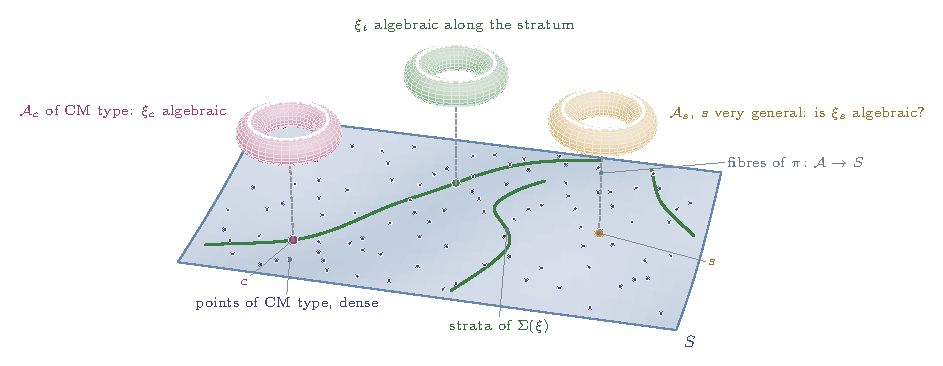
\includegraphics[width=\textwidth]{fig_cmseed}
\caption{\Cref{thm:f2propagation} in one family. The sheet is the base $S$
of a polarised abelian scheme $\pi\colon\cA\to S$ through a given Hodge
class, as in \Cref{prop:cmfamily}; the small dots are its points of CM type,
dense by \Cref{lem:cmdense}, and the green curves are strata of the algebraic
locus $\Sigma(\xi)$ of the flat class $\xi$ (\Cref{lem:algstrata}). Above
three points the fibres are drawn as tori, and the loop on each stands for
$\xi$, carried from fibre to fibre by parallel transport. At the CM member
$\cA_{c}$ the class is algebraic, and it stays algebraic along the stratum
through $c$. At a very general member $\cA_{s}$ it is algebraic exactly when
$\Sigma(\xi)$ has an interior point, and (F2) is the statement that this
happens in every such family.}
\label{fig:cmseed}
\end{figure}

\subsection{(F3$'$) and the part reached from abelian varieties}
\label{ssec:abpart}

\begin{definition}[The abelian part]\label{def:abpart}
For a smooth complex projective variety $X$ and $p\ge0$ let
$H^{2p}_{\mathrm{ab}}(X)\subseteq H^{2p}(X,\QQ)$ be the sum of the images of
the maps
$\Gamma_{*}\colon H^{k}(B,\QQ)\to H^{2p}(X,\QQ)$,
$y\mapsto\mathrm{pr}_{X*}([\Gamma]\cup\mathrm{pr}_{B}^{*}y)$, over all
complex abelian varieties $B$, the point included, all $k$, and all algebraic
cycles $\Gamma$ on $B\times X$ with rational coefficients and of the
codimension that lands in degree $2p$.
\end{definition}

\begin{proposition}[\textup{(F3$'$)} is a statement about the complement of
the abelian part]\label{prop:abpart}
Let $X$ be a smooth complex projective variety and $p\ge0$.
\begin{enumerate}[label=\textup{(\roman*)},leftmargin=2.6em,itemsep=2pt]
\item $H^{2p}_{\mathrm{ab}}(X)$ is a sub-Hodge structure of
  $H^{2p}(X,\QQ)$, spanned by the images of finitely many of the maps
  $\Gamma_{*}$.
\item $\mathrm{Ab}^{p}(X)=\Hdg^{p}(X)\cap H^{2p}_{\mathrm{ab}}(X)$.
\item Let $T^{2p}_{\mathrm{ab}}(X)$ be a complement of
  $H^{2p}_{\mathrm{ab}}(X)$ in $H^{2p}(X,\QQ)$ as a Hodge structure. Then
  \textup{(F3$'$)} holds for $X$ in degree $2p$ if and only if
  $T^{2p}_{\mathrm{ab}}(X)$ contains no nonzero Hodge class, in particular
  whenever the Hodge group of $T^{2p}_{\mathrm{ab}}(X)$ fixes no nonzero
  vector.
\item $X$ lies in the class $\mathcal{A}$ of \Cref{prop:f3prime}(iii) if and
  only if $T^{2p}_{\mathrm{ab}}(X)=0$ for every $p$ and the odd cohomology is
  reached in the same way.
\end{enumerate}
\end{proposition}

\begin{proof}
(i) An algebraic cycle $\Gamma$ of codimension $e$ on $B\times X$, with
$\dim B=b$, induces a morphism of Hodge structures
$H^{k}(B,\QQ)\to H^{k+2e-2b}(X,\QQ)(e-b)$, so its image is a sub-Hodge
structure; a sum of sub-Hodge structures is one, and a finite-dimensional
space is spanned by finitely many of them.

(ii) Every $\Gamma_{*}\beta$ with $\beta$ a Hodge class lies in both sets, so
$\mathrm{Ab}^{p}(X)$ is contained in the intersection. Conversely take
$(B_{j},\Gamma_{j},k_{j})$, $1\le j\le r$, as in (i), and let
\[
  \Phi=\sum_{j}\Gamma_{j*}\colon
  \bigoplus_{j}H^{k_{j}}(B_{j},\QQ)(t_{j})\longrightarrow
  H^{2p}_{\mathrm{ab}}(X),
\]
with the Tate twists $t_{j}$ that make it a morphism of pure Hodge structures
of weight $2p$; it is surjective. Polarisable Hodge structures form a
semisimple category, so $\Phi$ has a section $\sigma$ that is a morphism of
Hodge structures. For a Hodge class $\gamma\in H^{2p}_{\mathrm{ab}}(X)$ the
class $\sigma(\gamma)$ is of type $(p,p)$, so each component
$\beta_{j}\in H^{k_{j}}(B_{j},\QQ)$ is a Hodge class, $k_{j}$ being even, and
$\gamma=\sum_{j}\Gamma_{j*}\beta_{j}\in\mathrm{Ab}^{p}(X)$.

(iii) A complement exists by semisimplicity, and the Hodge classes of
$H^{2p}(X,\QQ)$ are the sums of those of the two summands; by (ii) the
Hodge classes of the first summand are $\mathrm{Ab}^{p}(X)$. So
$\Hdg^{p}(X)=\mathrm{Ab}^{p}(X)$ exactly when the second has none, and a
Hodge class of $T^{2p}_{\mathrm{ab}}(X)$ is a vector fixed by its Hodge group
\cite[\S3]{Del82}. (iv) is the definition of $\mathcal{A}$ read degree by
degree.
\end{proof}

So \textup{(F3$'$)} asks nothing of the abelian part, where by (ii) and
\Cref{prop:f2isab} the Hodge conjecture reduces to (F2), and it asks of the
complement that it carry no Hodge class. The abelian part contains every
algebraic class, taking $B$ a point, so under the Hodge conjecture the
complement carries none. To prove \textup{(F3$'$)} for $X$ in degree $2p$
without it, one has to show that every Hodge class of $X$ is a sum of
classes $\Gamma_{*}\beta$, that is, to construct algebraic cycles $\Gamma$
on products $B\times X$ that reach it, which is the step
\Cref{rem:f3primeopen} isolates.
\Cref{prop:f3prime}(iii), \Cref{prop:aclosure} and \Cref{thm:simplextype}
are cases in which the complement is zero, and \Cref{prop:k3powers} and
\Cref{prop:k3ntype} cases in which the conjecture itself makes its Hodge
classes algebraic.

\subsection{The first open case of (F3$'$) in families}\label{ssec:rmlocus}

The frontier of \textup{(F3$'$)} in \Cref{rem:f3primefrontier} begins with
$S\times S$ and $S^{[2]}$ for a K3 surface $S$ with real multiplication. These
surfaces come in families over Hermitian symmetric domains, and the argument
of \cite[Theorem~1.1]{paperI} applies to them with rational Hodge isometries in place of
isogenies.

\begin{setupenv}[A family with real multiplication]\label{setup:rm}
\enlargethispage{2pt}%
Let $E$ be a totally real field of degree $r\ge2$ and $T$ a finite-dimensional
$\QQ$-vector space with an action of $E$ and a nondegenerate symmetric form
$q$ for which $E$ acts by self-adjoint maps, so that $q=\Tr_{E/\QQ}q_{E}$ for
a unique $E$-bilinear form $q_{E}$. Put $m=\dim_{E}T\ge3$, and suppose that
$q_{E}$ has signature $(2,m-2)$ at one real place $\sigma_{1}$ of $E$ and is
negative definite at the others, and that $(T,q)$ embeds isometrically in
$\Lambda_{\QQ}$, where $\Lambda$ is the K3 lattice; write
$N=T^{\perp}\cap\Lambda$. Let $T_{1}=T\otimes_{E,\sigma_{1}}\RR$ and
\[
  \cD_{E}=\{\,[\omega]\in\PP(T_{1}\otimes_{\RR}\CC):\ q(\omega,\omega)=0,\
  q(\omega,\bar\omega)>0\,\}^{+},
\]
one of its two components, a bounded symmetric domain of dimension $m-2$. For
$\omega\in\cD_{E}$ let $S_{\omega}$ be a K3 surface with a marking
$H^{2}(S_{\omega},\ZZ)\cong\Lambda$ carrying $H^{2,0}(S_{\omega})$ to
$\CC\omega$, which exists by the surjectivity of the period map
\cite[Chs.~6--7]{Huy16}; it is projective, since $N$ has signature
$(1,21-rm)$ and so contains a class of positive square, which is of type
$(1,1)$ \cite[Ch.~8]{Huy16}. Each $e\in E$ acts on
$T_{1}\otimes\CC$ by the scalar $\sigma_{1}(e)$ and is self-adjoint, so it
preserves the Hodge decomposition of $T$, and $T\subseteq H^{2}(S_{\omega},\QQ)$
is a sub-Hodge structure containing $T(S_{\omega})_{\QQ}$. Write
$\tilde e_{\omega}\in H^{4}(S_{\omega}\times S_{\omega},\QQ)$ for the class of
the endomorphism $e\oplus0$ of $H^{2}(S_{\omega},\QQ)=T\oplus N_{\QQ}$, a
Hodge class, and let
\[
  \Sigma_{E}=\{\,\omega\in\cD_{E}:\ \tilde e_{\omega}\ \text{is algebraic
  for every}\ e\in E\,\}
\]
be the algebraic locus of the real multiplication; as $e\mapsto\tilde
e_{\omega}$ is $\QQ$-linear, it suffices to ask this for $e$ in a $\QQ$-basis
of $E$. The set $\Sigma_{E}$ does not depend on the choice of the surfaces
$S_{\omega}$. If $(S,\varphi)$ and $(S',\varphi')$ are two marked choices
for $\omega$, then $\psi=\varphi'^{-1}\varphi$ is a rational Hodge isometry
$H^{2}(S,\QQ)\to H^{2}(S',\QQ)$, induced by an algebraic class $Z$ on
$S\times S'$ by Buskin's theorem \cite{Bus19}, and $Z^{t}$ induces the
adjoint $\psi^{-1}$; the composite $Z\circ\tilde e\circ Z^{t}$ acts on
$H^{2}(S',\QQ)$ as $\psi(e\oplus0)\psi^{-1}$, which is $e\oplus0$ for the
marking $\varphi'$, and by zero on $H^{0}$ and $H^{4}$, so it is the class
$\tilde e'$ of $S'$, and $\tilde e$ is algebraic if and only if $\tilde e'$
is. Let $G=\Res_{E/\QQ}\SO(T,q_{E})$, so that
$G(\RR)=\SO(T_{1})\times\prod_{\sigma\ne\sigma_{1}}\SO(T_{\sigma})$; write
$G(\RR)^{+}$ for the identity component of this Lie group, which acts
transitively on $\cD_{E}$ through its first factor, and
$\Gamma_{\QQ}=G(\QQ)\cap G(\RR)^{+}$.
\end{setupenv}

The surfaces with real multiplication of \cite{vG08,vGS25} lie in families
of this kind,\footnote{For a projective K3 surface $S$ the transcendental
part $T(S)_{\QQ}$ is an irreducible Hodge structure whose algebra of Hodge
endomorphisms is a field, totally real or CM \cite{Zar83}; $S$ has real
multiplication when this field is totally real and not $\QQ$. The space
$T(S)_{\QQ}$ is then a vector space over the field, so its degree divides
$\dim T(S)_{\QQ}$, and a very general member of a family of
\Cref{setup:rm} has $T(S_{\omega})_{\QQ}=T$ and real multiplication by
exactly $E$, as the proof of \Cref{thm:rmlocus} shows.} and so do the surfaces $S_{\lambda}$ of \Cref{thm:mumfordks},
for which $E$ is cubic, $m=3$ and $\cD_{E}$ is a disc.

\begin{theorem}[The algebraic locus of a real multiplication]
\label{thm:rmlocus}
Keep \Cref{setup:rm}.
\begin{enumerate}[label=\textup{(\roman*)},leftmargin=2.6em,itemsep=2pt]
\item The points $\omega$ at which $S_{\omega}$ has complex multiplication,
  that is, at which the Hodge group of $T(S_{\omega})_{\QQ}$ is commutative,
  are dense in $\cD_{E}$, and they lie in $\Sigma_{E}$.
\item $\Sigma_{E}$ is stable under $\Gamma_{\QQ}$, and $\Gamma_{\QQ}$ is dense
  in $G(\RR)^{+}$.
\item $\Sigma_{E}$ is dense in $\cD_{E}$, and either $\Sigma_{E}=\cD_{E}$ or
  $\Sigma_{E}$ is meagre.
\item The following are equivalent: $\Sigma_{E}$ is closed; $\Sigma_{E}$ has
  an interior point; $\Sigma_{E}$ is not meagre; $\Sigma_{E}=\cD_{E}$; the
  Hodge conjecture holds for $S_{\omega}\times S_{\omega}$ for every $\omega$
  outside a countable union of proper closed analytic subsets of $\cD_{E}$.
  When they hold, the Hodge conjecture and \textup{(F3$'$)} hold for
  $S_{\omega}\times S_{\omega}$ and $S_{\omega}^{[2]}$ at every $\omega$ at
  which $\End_{\mathrm{Hdg}}(T(S_{\omega})_{\QQ})$ is $E$ or a CM field.
\end{enumerate}
\end{theorem}

\begin{proof}
We first record two facts about the very general point. The Hodge structure
of $S_{\omega}$ on $T$ is given by
$u_{\omega}\colon\mathrm{U}(1)\to\SO(T_{\RR})$, acting by $z^{2}$ on
$\CC\omega$, by $z^{-2}$ on $\CC\bar\omega$ and trivially on their orthogonal
complement; it commutes with $E$, lies in $G(\RR)^{+}$, and
$u_{g\omega}=gu_{\omega}g^{-1}$ for $g\in G(\RR)^{+}$.

(a) \emph{No nonzero $t\in T$ is orthogonal to every $\omega\in\cD_{E}$.} The
lines $\CC\omega$, $\omega\in\cD_{E}$, span $T_{1}\otimes\CC$, since
$\cD_{E}$ is a nonempty open subset of the nondegenerate quadric
$q(\omega,\omega)=0$ in $\PP(T_{1}\otimes\CC)$, so such a $t$
would have zero image in $T_{1}$; but $T\to T_{1}$ is injective, since $T$ is
a free $E$-module and $\sigma_{1}$ is injective.

(b) \emph{An endomorphism $f$ of $T$ that is an endomorphism of Hodge
structures at every $\omega\in\cD_{E}$ is multiplication by an element of
$E$.} Such an $f$ commutes with every $u_{\omega}$, hence with the elements
$X_{\omega}$ of the Lie algebra of $G(\RR)$ that span the Lie algebras of
the groups $u_{\omega}(\mathrm{U}(1))$. They lie in
$\mathfrak{so}(T_{1})\oplus0$, which acts on
$T'=\bigoplus_{\sigma\ne\sigma_{1}}T_{\sigma}$ by zero, and their span is
stable under $G(\RR)^{+}$, since $u_{g\omega}=gu_{\omega}g^{-1}$, so it is an
ideal of $\mathfrak{so}(T_{1})$. That ideal has nonzero projection to every
simple ideal, as the eigenvalues $2i,-2i,0,\dots,0$ of $X_{\omega}$ on
$T_{1}\otimes\CC$ show also for $m=4$, where
$\mathfrak{so}(T_{1})\otimes\CC\cong\mathfrak{sl}_{2}\oplus\mathfrak{sl}_{2}$
and $T_{1}\otimes\CC$ is the tensor product of the two standard
representations; so it is all of $\mathfrak{so}(T_{1})$, and $f$ commutes
with $\mathfrak{so}(T_{1})$. For $m\ge3$ the representation of
$\mathfrak{so}(T_{1})$ on $T_{1}\otimes\CC$ is irreducible and nontrivial, so
$f$ preserves $T_{1}=\mathfrak{so}(T_{1})\cdot T_{\RR}$ and $T'$ and acts on
$T_{1}\otimes\CC=T\otimes_{E,\sigma_{1}}\CC$ by a scalar $\lambda$. An
automorphism $\tau$ of $\CC$, acting on $T\otimes_{\QQ}\CC$ through the
second factor, commutes with $f$ and maps $T\otimes_{E,\sigma_{1}}\CC$ onto
$T\otimes_{E,\tau\sigma_{1}}\CC$, so $f$ acts on the latter by
$\tau(\lambda)$; and every embedding of $E$ is of the form $\tau\sigma_{1}$.
So $f\otimes1$ is multiplication by an element $e$ of $E\otimes_{\QQ}\CC$ on
$T\otimes_{\QQ}\CC=T\otimes_{E}(E\otimes_{\QQ}\CC)$, and $e$ is fixed by
$\mathrm{Aut}(\CC)$ because $f$ is defined over $\QQ$; hence $e\in E$.

For $t\in T$ the set of $\omega$ with $t\perp\omega$ is a closed analytic
subset of $\cD_{E}$, and for $f\in\End_{\QQ}(T)$ so is the set where $f$ is
an endomorphism of Hodge structures, namely where $f(\omega)\in\CC\omega$ and
$f^{*}(\omega)\in\CC\omega$, $f^{*}$ the adjoint. By (a) and (b) these sets
are proper for $t\ne0$ and $f\notin E$. There are countably many of them, and
outside their union $\NS(S_{\omega})_{\QQ}\cap T=0$, so
$T(S_{\omega})_{\QQ}=T$ and $\End_{\mathrm{Hdg}}(T(S_{\omega})_{\QQ})=E$.

(i) The Hodge group of $T$ acts trivially on $T\cap\NS(S_{\omega})_{\QQ}$,
whose orthogonal complement in $T$ is $P=T(S_{\omega})_{\QQ}$, so it is
commutative exactly when the Hodge group $H$ of $P$ is. The group $G$ is
connected and reductive, and $\omega\mapsto u_{\omega}$ identifies $\cD_{E}$
with the orbit of \Cref{lem:cmdense}, since $g\in G(\RR)^{+}$ fixes
$u_{\omega}$ exactly when it preserves the line $\CC\omega$, the eigenspace
of $u_{\omega}(z)$ for $z^{2}$. By \Cref{lem:cmdense} the points at which
$u_{\omega}(\mathrm{U}(1))$ lies in the real points of a maximal $\QQ$-torus of
$G$ are dense; at them the Hodge group of $T$, the smallest algebraic
$\QQ$-subgroup whose real points contain $u_{\omega}(\mathrm{U}(1))$, lies in
that torus, so these points have complex multiplication. Now let $\omega$ be
any point at which $H$ is commutative. The Hodge structure $P$ is
irreducible \cite{Zar83}, so $P$ is an irreducible representation of the
torus $H$, whose rational points are Zariski dense in it. The
$\QQ$-subalgebra $L$ of $\End(P)$ that $H(\QQ)$ generates is therefore
commutative, and $P$ is a simple faithful $L$-module; so $L$ is a field with
$\dim_{L}P=1$, and its commutant $E'=\End_{\mathrm{Hdg}}(P)$ is $L$. By
\cite{Zar83} $E'$ is totally real or CM. If it were totally real, the
embedding $\tau$ through which it acts on the line $H^{2,0}(S_{\omega})$
would be real, and that line would lie in $P\otimes_{E',\tau}\CC$, which is
one-dimensional and stable under complex conjugation, so it would also
contain the different line $H^{0,2}(S_{\omega})$, which is impossible. So
$E'$ is a CM field, the Hodge conjecture
holds for $S_{\omega}\times S_{\omega}$ by \Cref{prop:k3powers}(i), and the
Hodge classes $\tilde e_{\omega}$ are algebraic.

(ii) Let $g\in\Gamma_{\QQ}$ and $\omega\in\Sigma_{E}$. Then $g\omega\in\cD_{E}$,
and $\phi=\mathrm{id}_{N}\oplus g$ is a rational isometry of
$\Lambda_{\QQ}=N_{\QQ}\oplus T$ carrying $\CC\omega$ to $\CC g\omega$, so
through the markings it is a rational Hodge isometry
$H^{2}(S_{\omega},\QQ)\to H^{2}(S_{g\omega},\QQ)$, induced by an algebraic
class $Z\in H^{4}(S_{\omega}\times S_{g\omega},\QQ)$ \cite{Bus19}, whose
transpose induces $\phi^{-1}$. As $g$ is $E$-linear,
$\phi\circ(e\oplus0)\circ\phi^{-1}=e\oplus0$, so, as in \Cref{setup:rm},
$\tilde e_{g\omega}=Z\circ\tilde e_{\omega}\circ Z^{t}$ is algebraic.

For the density of $\Gamma_{\QQ}$, let $Y$ be an $E\otimes\RR$-linear map of
$T\otimes\RR$ that is skew-adjoint for $q$ and has $1-Y$ invertible. Its
Cayley transform $c(Y)=(1+Y)(1-Y)^{-1}$ is $E\otimes\RR$-linear, has
$c(Y)^{*}c(Y)=1$ because $1-Y$ is the adjoint of $1+Y$, and has determinant
one for the same reason, so $c(Y)\in G(\RR)$; and $c$ is a homeomorphism onto
the open neighbourhood $\{g\in G(\RR):1+g\ \text{invertible}\}$ of $1$, with
inverse $g\mapsto(g-1)(g+1)^{-1}$. The $E$-linear skew-adjoint maps of $T$
are dense among these $Y$, and $c$ maps them into $G(\QQ)$. So $\Gamma_{\QQ}$
is dense in a connected open neighbourhood of $1$, its closure is an open
subgroup of $G(\RR)^{+}$, and it is all of $G(\RR)^{+}$.

(iii) and (iv). Density follows from (i). If $\Sigma_{E}$ contains a nonempty
open set $U_{0}$, then $\Sigma_{E}=\cD_{E}$: for $\omega\in\cD_{E}$ choose
$\omega'\in U_{0}$ and $g_{1}\in G(\RR)^{+}$ with $g_{1}\omega'=\omega$; the
set of $g\in G(\RR)^{+}$ with $g^{-1}\omega\in U_{0}$ is open and contains
$g_{1}$, so by (ii) it contains some $g\in\Gamma_{\QQ}$, and
$\omega=g(g^{-1}\omega)\in\Sigma_{E}$ by (ii).

It remains to show that $\Sigma_{E}$ has an interior point as soon as it is
not meagre. Fix $h\in N$ with $h^{2}>0$ and $h\cdot\delta\ne0$ for every
$\delta\in N$ with $\delta^{2}=-2$, which exists because the hyperplanes
$\delta^{\perp}$ are locally finite in the positive cone of $N_{\RR}$
\cite[Ch.~8]{Huy16}. Let $\cD^{\circ}$ be the set of $\omega\in\cD_{E}$ that
are orthogonal to no $\delta\in\Lambda$ with $\delta^{2}=-2$ and
$h\cdot\delta=0$. Writing such a $\delta$ as $n+t$ with $n\in N_{\QQ}$ and
$t\in T$, we have $t\ne0$, because $N_{\QQ}\cap\Lambda=N$, and
$\delta\perp\omega$ exactly when $t\perp\omega$; so by (a) the complement of
$\cD^{\circ}$ lies in a countable union of proper closed analytic subsets and
is meagre.

Let $\omega\in\cD^{\circ}$. No class of $\NS(S_{\omega})$ of square $-2$ is
orthogonal to $h$, so after composing the marking with an isometry $\pm w$,
$w$ a product of reflections in such classes, which fixes $\omega$ and so
changes only the choice of $S_{\omega}$, the class $h$ is that of an ample
line bundle $L$ on $S_{\omega}$ \cite[Ch.~8]{Huy16}. The deformations of the
pair $(S_{\omega},L)$ form a smooth family over a base that the local period
map identifies with a neighbourhood of $\omega$ in the domain of periods
orthogonal to $h$ \cite[Ch.~6]{Huy16}, and that domain contains $\cD_{E}$,
since $h\in N$. Restricting to $\cD_{E}$, we obtain an open neighbourhood $U$
of $\omega$ in $\cD_{E}$ and a smooth family $\cX_{U}\to U$ of K3 surfaces with
markings, whose fibre over $u$ is a choice of $S_{u}$, carrying a line bundle
that restricts to $L$ on $S_{\omega}$. On $S_{\omega}$ the bundle
$L^{\otimes3}$ is very ample and has no higher cohomology
\cite[Ch.~2]{Huy16}; by semicontinuity and base change, after shrinking $U$,
its direct image is free and its sections embed $\cX_{U}$ in
$\PP^{M}\times U$ over $U$. The classes $\tilde e$ are flat sections of the
fourth cohomology of $\cX_{U}\times_{U}\cX_{U}$, which is projective over $U$.
As in the proof of \Cref{lem:algstrata}(i), with the Hilbert schemes of
$\PP^{M}\times\PP^{M}$ \cite{Gro61}, which are projective, for each $e$ in a
$\QQ$-basis of $E$ the set of $u\in U$ at which
$\tilde e_{u}=\sum_{i}q_{i}[Z_{i}]$ with rational $q_{i}$ and $Z_{i}$ of
Hilbert polynomial $P_{i}$ is the image, under a proper map, of a union of
connected components of a fibre product of relative Hilbert spaces over $U$,
and so it is closed in $U$. Taking the union over the countably many
$(\underline{P},\underline{q})$ and the intersection over the basis,
$\Sigma_{E}\cap U$ is a countable union of subsets of $U$ that are closed in
$U$.

The sets $U$ constructed for the points of $\cD^{\circ}$ cover it, and
countably many of them, $U_{i}$, suffice, since $\cD_{E}$ has a countable
basis. If $\Sigma_{E}$ is not meagre, neither is
$\Sigma_{E}\cap\cD^{\circ}$, so some $\Sigma_{E}\cap U_{i}$ is not meagre, and
by the Baire category theorem in $U_{i}$ one of the countably many closed
subsets of $U_{i}$ that make it up has an interior point. This proves (iii),
and in (iv) the equivalence of the first four conditions, since a dense
closed set is everything. The fifth condition implies the third, because at
each point where the Hodge conjecture holds for $S_{\omega}\times S_{\omega}$
the Hodge classes $\tilde e_{\omega}$ are algebraic, and the complement of a
countable union of proper closed analytic subsets is not meagre.

If $\Sigma_{E}=\cD_{E}$ and $\End_{\mathrm{Hdg}}(T(S_{\omega})_{\QQ})=E$, then
$E$ preserves $T(S_{\omega})_{\QQ}$, the smallest sub-Hodge structure of $T$
whose complexification contains $H^{2,0}(S_{\omega})$, since each $e\ne0$
maps it onto a sub-Hodge structure of the same dimension that contains
$H^{2,0}(S_{\omega})$; and each $e\in E$ acts
on it through the algebraic class $\pi_{T}\circ\tilde e_{\omega}\circ\pi_{T}$,
where $\pi_{T}$ is the algebraic projector onto $T(S_{\omega})_{\QQ}$ of the
proof of \Cref{prop:k3powers}; so \Cref{prop:k3powers}(iii) gives the Hodge
conjecture for $S_{\omega}\times S_{\omega}$ and $S_{\omega}^{[2]}$, and with
it \textup{(F3$'$)}. If the field is CM, \Cref{prop:k3powers}(i) gives the
same. Outside the countable union found at the beginning of the proof the
field is $E$, so the fourth condition implies the fifth.
\end{proof}

On the families of van Geemen and Sch\"utt with real multiplication by
$\QQ(\zeta_{7}+\zeta_{7}^{-1})$ and $\QQ(\zeta_{9}+\zeta_{9}^{-1})$ the
real multiplication is induced by explicit cycles \cite[Theorem~1.2 and
Section~4.8]{vGS25}, and on the double planes branched along six lines that
have real multiplication, necessarily by a quadratic field here, by
Schlickewei's cycles \cite{Sch10,vG08}. Whenever the members on which such
cycles are known contain a nonempty open subset of $\cD_{E}$, (iv) gives
$\Sigma_{E}=\cD_{E}$. For the family of the surfaces $S_{\lambda}$,
\Cref{thm:rmlocus} gives the real multiplication at every CM point and on a
dense set stable under $\Gamma_{\QQ}$, and \Cref{thm:mumfordks}(ii) gives it
at $S_{\lambda}$ if the Kuga--Satake class of $S_{\lambda}$ is algebraic;
whether $\Sigma_{E}$ is closed there is open. Since $\Sigma_{E}$ is stable
under the group $\Gamma_{\QQ}$, every $\Gamma_{\QQ}$-orbit lies either in
$\Sigma_{E}$ or in its complement: the Hodge isometries of (ii) move the real
multiplication along an orbit and never bring it to an orbit where it is not
yet algebraic, and by \Cref{rem:mumfordks} the composites of Hodge
similarities that return to $T(S_{\lambda})$ span only the maximal
multiquadratic subfield of $E$, which is $\QQ$ for a cubic field.

\subsection{What the constructions reach}\label{ssec:reach}

\begin{theorem}[Where (F2) and (F3$'$) stand]\label{thm:twostand}
\leavevmode
\begin{enumerate}[label=\textup{(\roman*)},leftmargin=2.6em,itemsep=3pt]
\item \emph{What carries over.} In every polarised abelian scheme of
  \Cref{thm:f2propagation} the algebraic locus of a flat class is a
  countable union of closed algebraic strata and is either everything or
  meagre (\Cref{lem:algstrata}); in the Weil families it is moreover dense
  and contains an explicit CM point (\cite[Theorem~1.1]{paperI}); in every family of
  \Cref{setup:rm} the algebraic locus of the real multiplication is dense,
  contains every CM point, is stable under $\Gamma_{\QQ}$ and is either
  everything or meagre (\Cref{thm:rmlocus}); and every Hodge class of every
  abelian variety lies in a polarised abelian scheme with a CM member
  (\Cref{prop:cmfamily}).
\item \emph{(F2).} It holds if and only if the algebraic locus of every flat
  Hodge class algebraic at a CM member of a polarised abelian scheme has an
  interior point (\Cref{thm:f2propagation}). In the Weil families the
  constructions of the paper that supply an interior point are: an object
  with injective semiregularity map, or satisfying the flatness condition,
  at one point (\cite[Theorem~2.3]{paperII}, \cite[Theorem~17.7]{paperI},
  \cite[Proposition~3.15]{paperII}); a bound on the Hilbert data of representatives along
  the Hecke orbit of a base point (\cite[Theorem~16.9]{paperI}), which is
  equivalent to its conclusion (\cite[Theorem~16.17]{paperI}); and the Lefschetz
  standard conjecture for the total space over a curve through a base point,
  which implies it and, when the monodromy is Zariski dense, follows from it
  (\Cref{cor:weilequiv}). For the squares of Mumford fourfolds the last two
  take the forms of \Cref{thm:modpdensity} and \Cref{cor:mumfordequiv}.
  Markman's sheaves are objects of the first kind, and with them he proves
  the algebraicity of the Weil classes on every abelian fourfold of Weil
  type and on the split sixfolds of every imaginary quadratic field
  \cite{Mar25a,Mar25b}; with \cite{MZ99} this gives the Hodge conjecture for
  abelian varieties of dimension at most five. The open cases named in
  \Cref{sec:scope} include the non-split Weil sixfolds of imaginary
  quadratic fields, the Weil eightfolds of quartic CM fields, where an
  object of the first kind needs
  $\dim\Ext^{2}(E,E)\ge88$ (\cite[Corollary~5.15]{paperII}), and the squares of
  Mumford fourfolds, where the classes are algebraic at every CM point
  (\Cref{thm:mumfordcm}) and on every member once one Kuga--Satake class is
  algebraic (\Cref{thm:mumfordks}), or once one complex at one CM point has
  $\Ext^{2}$ of dimension $119$ (\Cref{thm:mumfordnumerical}); on the
  square of a Mumford fourfold the two exceptional classes are algebraic
  exactly when one class on a product with an abelian sixfold is
  (the sixfold link of \cite{BB26dense}).
\item \emph{(F3$'$).} It holds if and only if, for every variety and every
  degree, the complement of the abelian part carries no Hodge class
  (\Cref{prop:abpart}). The complement is zero on the class $\mathcal{A}$,
  which contains the Fermat and Delsarte hypersurfaces of every dimension and
  the cyclic covers branched along them (\Cref{prop:aclosure},
  \Cref{cor:delsarteall}), and it carries no Hodge class on the varieties of
  \Cref{prop:f3primesmall}, \Cref{prop:f3primefibration} and
  \Cref{prop:f3primedominant}, where \textup{(F3$'$)} is proved, and of
  \Cref{prop:k3powers} and \Cref{prop:k3ntype}, where the conjecture itself
  is.
  On the first open varieties, $S\times S$ and $S^{[2]}$ for a K3 surface
  with real multiplication, the algebraic locus of the real multiplication
  is dense, contains every CM point and is either the whole family or meagre
  (\Cref{thm:rmlocus}); the real multiplication is algebraic on the members
  of the families of \cite{vGS25} and on the quadratic double planes of
  \cite{Sch10}, and whether the locus is closed is open for the family of
  $S_{\lambda}$, except for the two cyclic cubic fields of conductor $7$
  and $9$ with the algebra split at one real place, where
  the dihedral correspondences of \cite{BB26dense} make the locus the
  whole family. Beyond the
  varieties of abelian type, a Hodge
  class off the abelian part is removed only by a new algebraic cycle on a
  product $B\times X$ (\Cref{rem:f3primeopen}).
\end{enumerate}
Neither (F2) nor \textup{(F3$'$)} is proved here, and by \Cref{thm:final}
together they are the Hodge conjecture.
\end{theorem}

\begin{proof}
Each statement is the result cited with it. For (ii), Markman's theorems are
recalled in the introduction and their reach in \Cref{sec:scope}, where the
non-split sixfolds and the fields of degree at least four are among the open
entries, and \cite[Theorem~5.14]{paperII} and
\cite[Corollary~5.15]{paperII} give the number $88$. For (iii), the known cases of
the real multiplication are those recalled in \Cref{rem:mumfordks}.
\end{proof}

\section{The closure theorem}\label{sec:final}

We collect the results of the paper in one theorem. Its first clause is
\cite[Theorem~1.1]{paperI}; the second and third give the base of that theorem in its
sharpest form; the fourth and fifth say what closing the algebraic locus
requires and which constructions cannot supply it; and the last places the
Weil classes inside the Hodge conjecture and states what \cite[Theorem~1.1]{paperI}
becomes when it is carried to every family. The theorems we quote from the
literature are used as theorems: the semiregularity theorem of Buchweitz and
Flenner \cite{BF03}, in the form for perfect complexes that Pridham proves
\cite{Pri24}; the theorem of Cattani, Deligne and Kaplan \cite{CDK95}; the
theorem of Baily and Borel \cite{BB66}; the theorem of Pila, Shankar and
Tsimerman on the Andr\'e--Oort conjecture \cite{PST}; the description of the
Hodge rings of abelian varieties of dimension at most five by Moonen and Zarhin
\cite{MZ99}; Markman's theorems on abelian varieties of Weil type
\cite{Mar25a,Mar25b}; the theorem of Bando and Siu on stable reflexive
sheaves \cite{BS94}, Kuranishi's theorem in the form of Goldman and Millson
\cite{Kur65,GM88}, Grivaux's Chern classes of coherent sheaves \cite{Gri10}
and Voisin's theorem on Weil tori \cite{Voi02b}; and the theorems of Deligne,
Andr\'e and Milne recorded in \Cref{ssec:bullseye}
\cite{Del71,And96b,Mil20}.

\begin{theorem}[Closure]\label{thm:final}
Let $F$ be a CM field of degree $2m$, let $n\ge2$, and let $\delta$ be a
discriminant. Write $K=\QQ(\sqrt{-d})$ when $m=1$.
\begin{enumerate}[label=\textup{(\roman*)},leftmargin=2.8em,itemsep=4pt]
\item \emph{The algebraic locus.} The algebraic locus $\Sigma_{F}$ of the Weil
  classes contains an explicit CM point at which they are polynomials with
  rational coefficients in divisor classes, it is dense, it is a countable
  union of closed algebraic strata, and it is either the whole domain or
  meagre. It is closed if and only if the Hodge conjecture holds for the very
  general member of the family, and then the Weil classes are algebraic on
  every member (\cite[Theorem~1.1]{paperI}).
\item \emph{One class on one connected domain.} For an abelian $2n$-fold $A$ of
  $(K,-1,n)$-Weil type with $\Hg(A)=\SU(V,H)$ one has
  $\dim_{\QQ}\Hdg^{k}(A)=1$ for $k\ne n$ and $3$ for $k=n$, and the Hodge
  conjecture for $A$ in every degree is the algebraicity of the single class
  $\omega_{1}$ of \cite[(11)]{paperI}, written out with $2^{2n-1}$ integer
  coefficients. For the family of the triple $(K,n,\delta)$ the conjecture is
  equivalent to the algebraicity of the absolutely Hodge class $\omega_{s}$ at
  every point $s$ of the connected period domain $\cD_{n,n}$ of dimension
  $n^{2}$ (\cite[Theorem~4.14]{paperI}, \cite[Corollary~4.15]{paperI}, \cite[Theorem~15.14]{paperI},
  \cite[Corollary~15.35]{paperI}).
\item \emph{A base point in every family.} Every family of every CM field
  contains a member isogenous to a product of CM abelian $m$-folds at which
  the Weil classes are polynomials in divisor classes
  (\cite[Theorem~17.5]{paperI}). For an imaginary quadratic field every family also
  contains a member with quaternionic multiplication extending $K$, at which
  the Weil classes are the real and imaginary parts of the $n$-th power of one
  explicit $(1,1)$ class, and every product of $n$ abelian surfaces of Weil
  type is a member whose Weil classes are an explicit integral polynomial in
  $2n$ divisor classes (\cite[Theorem~15.25]{paperI}, \cite[Theorem~15.27]{paperI},
  \cite[Theorem~15.10]{paperI}).
\item \emph{Closing the locus.} If at every point of the orbit
  $G_{F}(\QQ)\cdot s_{0}$ the Weil class is represented by a cycle whose
  Hilbert data comes from one finite set, then $\Sigma_{F}=\cD_{F}$; this
  hypothesis is equivalent to its conclusion, and the transported cycle does
  not satisfy it whenever a component of the base cycle has finite stabiliser
  (\cite[Theorem~16.9]{paperI}, \cite[Theorem~16.17]{paperI}, \cite[Theorem~16.15]{paperI}).
  The bound is needed only along one sequence of CM points that leaves every
  proper special subvariety, and such a sequence exists inside the orbit
  (\cite[Theorem~17.14]{paperI}). The locus of members with smaller Hodge group, which
  contains every member at which this paper exhibits algebraic Weil
  classes, contains the base point, is dense, stable under
  $G_{F}(\QQ)$ and a countable union of closed algebraic strata, and is
  meagre, so closing the locus requires the algebraicity of the Weil classes
  at a member with full Hodge group (\cite[Proposition~17.12]{paperI}, \cite[Corollary~17.13]{paperI}). If
  at a base point some perfect complex whose Chern character is a nonzero
  multiple of a rational Weil class plus a polynomial in the divisor classes
  of the family has injective semiregularity map, or satisfies the flatness
  condition of \cite[Proposition~3.15]{paperII}, then $\Sigma_{F}=\cD_{F}$
  (\cite[Theorem~2.3]{paperII}, \cite[Theorem~17.7]{paperI}). When the Chern
  character is exactly a multiple of a Weil class, no complex at any member of
  any family, for any CM field, has injective semiregularity map
  (\cite[Theorem~3.5]{paperII}, \cite[Theorem~5.4]{paperII}). In the polarised form, for an
  imaginary quadratic field and $n\ge3$, every object has
  $\dim\Ext^{2}(E,E)\ge(4+\rho)n^{2}-2n$, with $\rho\le3$ the rank of the
  Hankel matrix of the coefficients, and an object attaining the bound meets
  the criterion (\cite[Theorem~3.9]{paperII}); at a quartic
  CM field and $n=2$ the number takes fifteen values, an object meeting the
  criterion has $\dim\Ext^{2}(E,E)\ge88$, and the characters of rank $88$
  whose Hodge locus leaves the polarised family are exactly those of
  $\theta^{4}$ shape, which the Weil tori exclude (\cite[Theorem~5.14]{paperII},
  \cite[Corollary~5.15]{paperII}, \cite[Proposition~5.17]{paperII},
  \cite[Corollary~5.18]{paperII}). The statement is needed only for the split
  families of the CM fields of degree at least four, which carry the Weil
  classes of every CM field by descent and scalar extension
  (\Cref{prop:descent}), and for one family it is equivalent to the Lefschetz
  standard conjecture for the total space of the family over a curve through a
  base point (\Cref{cor:weilequiv}).
\item \emph{Constructions that do not reach a Weil class.} Each of the
  following fails to produce a Weil class on a general member, in the sense
  and under the hypotheses of the theorem cited, which \Cref{sec:scope}
  delimits:
  \begin{enumerate}[label=\textup{(\alph*)},nosep,leftmargin=2.2em]
  \item an object restricted from a projective space to the dual and
    transported by the Poincar\'e kernel (\cite[Theorem~7.3]{paperI});
  \item equivariant for the field with the norm character
    (\cite[Theorem~5.6]{paperI});
  \item an object whose Chern character lies on the Weil line and on which
    $H^{2}(\cO_{A})$ acts faithfully, whether through semiregularity or
    through the weakened criterion of \cite[Question~11.4]{Mar25b}
    (\cite[Theorem~9.7]{paperI}, \cite[Corollary~9.18]{paperI}, \cite[Theorem~9.19]{paperI});
  \item an object with a line bundle summand off the polarisation line, in
    particular a sum of line bundles (\cite[Theorem~9.20]{paperI},
    \cite[Corollary~4.21]{paperII});
  \item an object whose Chern character is effective at a base point
    (\cite[Theorem~4.5]{paperII});
  \item induction through hyperplane sections, in either direction
    (\cite[Theorem~10.3]{paperI}, \cite[Theorem~10.8]{paperI});
  \item Kuga--Satake from a weight two sub-structure of $H^{2}(A,\QQ)$
    (\cite[Proposition~11.11]{paperI}, \cite[Corollary~11.12]{paperI});
  \item a divisorial argument at a general member of a family of nontrivial
    discriminant (\cite[Proposition~15.18]{paperI});
  \item a secant object whose support has two smooth branches of codimension
    two meeting transversally at a point, which includes the candidate of
    \cite[Section~12]{Mar25b} (\cite[Theorem~4.61]{paperII},
    \cite[Corollary~4.63]{paperII}, \cite[Corollary~4.77]{paperII});
  \item a secant object of rank one whose support is a complete intersection
    of two divisors (\cite[Theorem~4.81]{paperII}), or a secant object quasi-isomorphic to
    a two-term complex of sums of powers of the polarisation or of simple
    semi-homogeneous bundles (\cite[Theorem~4.89]{paperII}, \cite[Theorem~4.92]{paperII}); on
    the fourfold, a secant sheaf $\cI_{S}(3\Theta)$ with smooth support
    unless $d\le9$, that is $d\in\{1,3,5,7\}$ in \cite[Setup~4.51]{paperII}, and
    one whose ideal sheaf is presented by two bundles
    with classes in the subring generated by line bundles unless
    $d\equiv15,23\pmod{24}$ (\cite[Corollary~4.68]{paperII},
    \cite[Corollary~4.84]{paperII});
  \item a representative of the Weil $K$-theory class that is a locally free
    sheaf on a smooth germ of codimension at least two of its support, or
    whose support has codimension at least $n$ (\cite[Theorem~2.5]{paperII},
    \cite[Theorem~2.13]{paperII});
  \item at a quartic CM field, a complex with secant character that is
    locally free on a smooth curve at some point, in particular the explicit
    pair of \cite[Example~11.2.7]{Mar25c} (\cite[Theorem~5.28]{paperII},
    \cite[Corollary~5.30]{paperII});
  \item a convolution of fewer than $2n$ line bundles with nondegenerate
    differences (\cite[Theorem~4.26]{paperII}); on $E_{0}^{6}$, every convolution
    of the Weil pieces with three multiples of the polarisation, and on
    $E_{0}^{8}$ every one whose pieces have their shifts within six
    consecutive values (\cite[Theorem~4.35]{paperII}, \cite[Corollary~4.48]{paperII}).
  \end{enumerate}
\item \enlargethispage{4pt}\emph{The Weil classes inside the conjecture.} The Hodge conjecture is
  equivalent to the conjunction of \textup{(F2)}, the algebraicity of the
  Hodge classes of abelian varieties outside the subring generated by divisor
  classes and Weil classes of quotients, and \textup{(F3$'$)}, the
  algebraicity of every Hodge class modulo the images of Hodge classes of
  abelian varieties under algebraic correspondences; and \textup{(F2)} alone
  is equivalent to the Hodge conjecture for abelian varieties
  (\Cref{prop:f2isab}, \Cref{prop:f3prime}). The statement \textup{(F3$'$)}
  holds on every variety whose cohomology is reached from abelian varieties by
  correspondences, on every variety of dimension at most three, on every
  fourfold and fivefold whose zero-cycles are supported in dimension at most
  three or that is dominated by a variety of the first kind, on every smooth
  ample divisor of odd dimension in a variety of the first kind, and on every
  smooth Delsarte hypersurface of every dimension and every cyclic cover
  branched along one, and on every complete intersection of diagonal
  hypersurfaces of Vandermonde type, where the Hodge conjecture follows for
  two diagonal hypersurfaces of degree $3$, $4$ or $6$ in $\PP^{6}$ and for
  the very general member of degree $2$ in every dimension, of degree $3$ or
  $4$ up to dimension seven and of degree $6$ up to dimension five
  (\Cref{prop:f3prime}, \Cref{prop:aclosure},
  \Cref{prop:f3primesmall}, \Cref{prop:f3primefibration},
  \Cref{prop:f3primedominant}, \Cref{prop:f3primeample}, \Cref{cor:delsarteall},
  \Cref{thm:vandermonde}, \Cref{cor:twodiagonal},
  \Cref{thm:vgvandermonde}). The first instance of
  \textup{(F2)}, the two exceptional classes on the square of a Mumford
  fourfold, is algebraic at every CM point of the family, is algebraic on
  every member once one Kuga--Satake class is algebraic, and is algebraic on
  every member exactly when the Lefschetz standard conjecture holds for one
  ninefold (\Cref{thm:mumfordcm}, \Cref{thm:mumfordks},
  \Cref{cor:mumfordequiv}). Over the rule set formed by the implications of
  the paper and of the literature, together with \Cref{prop:f2isab}, the
  minimal sets of statements from which the conjecture follows are
  $\{\mathrm{F3}\}$, $\{\mathrm{L},\mathrm{M}\}$,
  $\{\mathrm{L},\mathrm{F3}'\}$, $\{\mathrm{V},\mathrm{F3}'\}$ and
  $\{\mathrm{F2},\mathrm{F3}'\}$, the first two being each equivalent to it
  (\Cref{thm:closure}, \Cref{rem:f2rule}). Carried to every family,
  \cite[Theorem~1.1]{paperI} gives exactly these two statements back:
  \textup{(F2)} is equivalent to the statement that in every polarised
  abelian scheme with a member of CM type the algebraic locus of a flat
  Hodge class that is algebraic at such a member has an interior point
  (\Cref{thm:f2propagation}); \textup{(F3$'$)} is equivalent to the absence
  of Hodge classes off the part of the cohomology reached from abelian
  varieties by algebraic correspondences (\Cref{prop:abpart}); and on the
  squares of K3 surfaces with real multiplication, the first varieties on
  which \textup{(F3$'$)} is open, the algebraic locus of the real
  multiplication is dense, contains every CM point and is either the whole
  family or meagre (\Cref{thm:rmlocus}), and it is the whole family for
  real multiplication by $\sqrt2$, $\sqrt3$ and $\sqrt6$ in families, for
  complex multiplication by $\QQ(\sqrt{-5})$ and $\QQ(\sqrt{-7})$ on the
  Fricke families, and for the cubic fields $\QQ(\zeta_{7})^{+}$ and
  $\QQ(\zeta_{9})^{+}$ on the surfaces of the Mumford fourfolds of the
  algebra split at one real place \cite{BB26dense}.\footnote{These are the statements
  \textup{(L)}, \textup{(M)} and \textup{(V)} of \Cref{def:lmv}: $B(X)$ of
  \cite[Definition~10.6]{paperI} for every smooth projective $X$; every Hodge class
  motivated in the sense of Andr\'e \cite[\S2.1]{And96b}; and, for every
  smooth projective morphism $f$ to a smooth connected base, a flat section of
  $R^{2p}f_{*}\QQ$ that is algebraic at one point is algebraic at every
  point. The statement (F3) is the Hodge conjecture for the varieties that
  are not abelian, which is equivalent to the whole conjecture
  (\Cref{prop:f3ishc}).}
\end{enumerate}
\end{theorem}

\begin{proof}
Each clause is the theorem or theorems cited with it, and no clause is used
in the proof of another. For (i), \cite[Theorem~1.1]{paperI} is proved at the end of
\cite[Section~17.3]{paperI}. For (ii), \cite[Theorem~4.14]{paperI} counts the Hodge
classes, \cite[Corollary~4.15]{paperI} reduces every degree to $\omega_{1}$,
\cite[Theorem~4.9(i)]{paperI} shows that $\omega_{1}$ has integer coefficients
and exactly $2^{2n-1}$ nonzero terms, \cite[Theorem~15.14(a)]{paperI} and (b) are the
two implications for the family, and \cite[Proposition~B.8]{paperI} gives the
connectedness and the dimension. For (iii), \cite[Theorem~17.5]{paperI} gives the
CM point, \cite[Theorem~15.25(v)]{paperI} the cycle at a quaternionic point,
\cite[Theorem~15.27]{paperI} places such a point in every family by the
discriminant computation of \cite[Theorem~15.25(iv)]{paperI} and \cite[Lemma~15.26]{paperI},
and \cite[Theorem~15.10]{paperI} treats products.

For (iv), the bounded criterion is \cite[Theorem~16.9]{paperI} with
\cite[Theorem~16.17]{paperI} and \cite[Theorem~16.15]{paperI}, and its form for a CM field
is \cite[Theorem~17.7(iv)]{paperI}; the escaping sequence is \cite[Theorem~17.14]{paperI},
and the special locus is \cite[Proposition~17.12]{paperI} with
\cite[Corollary~17.13]{paperI}. The semiregularity criterion is
\cite[Theorem~2.3]{paperII} with \cite[Remark~3.6]{paperII}, carried to every CM field
by \cite[Theorem~17.7(v)]{paperI}; the flatness form is \cite[Proposition~3.15]{paperII}. The
pure form is excluded by \cite[Theorem~3.5]{paperII}, which rests on
\cite[Lemma~3.2]{paperII}, \cite[Lemma~3.3]{paperII} and
\cite[Proposition~3.4]{paperII}, and for every CM field by
\cite[Theorem~5.4]{paperII}. The number of the polarised form is
\cite[Theorem~3.9(i)]{paperII},
(iv) and (v); the quartic rank and the Hodge loci are
\cite[Theorem~5.14]{paperII}, \cite[Corollary~5.15]{paperII}, \cite[Proposition~5.17]{paperII}
and \cite[Corollary~5.18]{paperII}. The reduction to the split families is
\Cref{prop:descent}, and the equivalence with the Lefschetz standard
conjecture is \Cref{cor:weilequiv}. For (v), each item is the statement of
the theorem cited, under its own hypotheses, which \Cref{sec:scope} delimits
item by item.

For (vi), \Cref{prop:f3prime}(i) gives the Hodge conjecture from
\textup{(F3$'$)} and the conjecture for abelian varieties, and
\Cref{prop:f2isab} gives the latter from \textup{(F2)}; the converse
implications hold because \textup{(F2)} is a case of the conjecture and
\textup{(F3$'$)} is weaker than it. The cases of \textup{(F3$'$)} are
\Cref{prop:f3prime}(iii) and (iv), \Cref{prop:aclosure},
\Cref{prop:f3primesmall}, \Cref{prop:f3primefibration},
\Cref{prop:f3primedominant}, \Cref{cor:delsarteall},
\Cref{thm:vandermonde}, \Cref{cor:twodiagonal} and \Cref{thm:vgvandermonde}.
The statements on
the Mumford classes are \Cref{thm:mumfordcm}, \Cref{thm:mumfordks}(ii) and
\Cref{cor:mumfordequiv}. The statements on the families are
\Cref{thm:f2propagation}, \Cref{prop:abpart} and \Cref{thm:rmlocus}; the
families on which the real multiplication is algebraic are treated in
\cite{BB26dense}. The
minimal sets are \Cref{thm:closure}(ii) with
the rule of \Cref{prop:f2isab} adjoined, as computed in \Cref{rem:f2rule},
and \Cref{thm:closure}(vi) shows that $\{\mathrm{F3}\}$ and
$\{\mathrm{L},\mathrm{M}\}$ are each equivalent to the conjecture.
\end{proof}

The theorem arranges the paper around \cite[Theorem~1.1]{paperI}. Clause (ii) is the
problem in its smallest form, one explicitly written class on one connected
domain, and clause (iii) shows that the base case is never the difficulty:
every family has a base point, for every field, every dimension and every
discriminant, with a cycle written down rather than an existence statement.
Clause (iv) reduces the closedness of the locus to one object at one point
and computes the number that object must attain, and clause (v) shows that
the constructions that fail do so for identifiable structural reasons: a
divisor-generated Chern character cannot leave the divisor subring, a norm
eigenclass sits in the wrong summand of the character grading, a Chern
character on the Weil line has an annihilator exactly as large as the family,
a support with two transversal branches of codimension two through a point
carries a local obstruction that the compensating scalar cannot meet, and a curve along which an object is locally
free is tangent to at most one of the two eigenplanes of the real
multiplication. Clause (vi) shows where the Weil classes stand in the whole
conjecture: the conjecture for abelian varieties is carried by the classes
beyond the Weil lines, and the rest is algebraicity modulo abelian varieties,
which holds on every variety whose cohomology comes from abelian varieties,
on the Delsarte hypersurfaces of every dimension and on the diagonal
complete intersections of Vandermonde type (\Cref{fig:twohalves}).
\Cref{sec:families} shows that the structure \cite[Theorem~1.1]{paperI} finds in the
Weil families, a CM seed, density and the dichotomy, is present in every
family that carries (F2) or \textup{(F3$'$)}, and that in each of them the
one missing property is the interior point that closes the locus
(\Cref{thm:twostand}).

\begin{figure}[tbp]
\centering
  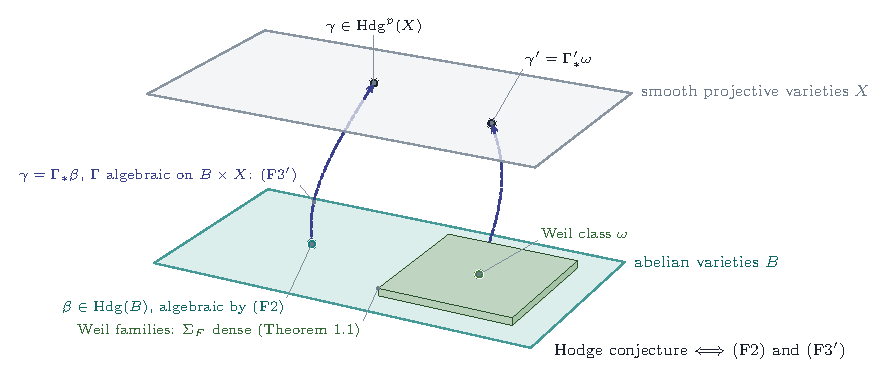
\includegraphics[width=\textwidth]{fig_twohalves}
\caption{The two halves of the conjecture in \Cref{thm:final}(vi). A Hodge
class $\gamma$ on a smooth projective variety $X$ is the image
$\Gamma_{*}\beta$ of a Hodge class $\beta$ on an abelian variety $B$ under an
algebraic correspondence $\Gamma$ on $B\times X$, which is \textup{(F3$'$)};
the class $\beta$ is algebraic, which is \textup{(F2)}, equivalently the
conjecture for abelian varieties (\Cref{prop:f2isab}). The raised plate on
the lower sheet stands for the families of Weil type, on which
\cite[Theorem~1.1]{paperI} makes the algebraic locus of the Weil class $\omega$ dense;
the dashed part of each correspondence is the part behind the upper sheet.}
\label{fig:twohalves}
\end{figure}


% \zenodoCodeID is the DOI the paper cites for the archive of the earlier
% paper on Weil classes, in the data availability section and in the entry
% BMB26 of the bibliography: the version DOI of release v5.0.1 of that
% archive, a version of the concept record 10.5281/zenodo.22950275.
\newcommand{\zenodoCodeID}{10.5281/zenodo.23225483}
\newcommand{\zenodoCodeDOI}{%
  \href{https://doi.org/\zenodoCodeID}{\texttt{\zenodoCodeID}}}

\section*{Acknowledgements}
The paper builds on the theorems of Eyal Markman on secant sheaves and Weil
classes, on the semiregularity theory of Spencer Bloch, Ragnar-Olaf
Buchweitz and Hubert Flenner, and on the descriptions of Hodge classes on
abelian varieties by Ben Moonen, Yuri Zarhin, Yves Andr\'e and James Milne.
We thank Priyabrata Mandal for the collaboration on the earlier paper on
Weil classes, whose results this paper and its companions \cite{paperI,paperII} divide between them.

\section*{Declarations}

\subsection*{Funding}
The authors received no funding for this work.

\subsection*{Competing interests}
The authors have no competing interests to declare.

\subsection*{Ethics approval and consent}
This article reports no research involving human participants, human data or
animals, so ethics approval and consent to participate or to publish were not
required. The results are original and have not been published elsewhere
except in the earlier paper named on the title page, which this paper and its
companions replace, and the work of others is credited by citation throughout.

\subsection*{Data availability}
The archive \cite{BMB26} is deposited on Zenodo under the DOI
\zenodoCodeDOI. It holds programs that repeat much of the finite arithmetic of this paper and its companions \cite{paperI,paperII}
as an independent check, a Lean~4 certificate of part of that arithmetic, the
Macaulay2 computations of local $\Ext$ algebras with their output, and the
generators and TikZ sources of the figures; its programs perform $2218$
checks, all of which pass, and the Lean kernel checks four hundred and nine
theorems, each depending on no axiom or on propositional extensionality
alone. Deep Bhattacharjee computed all the calculations, in C, Python, Julia,
Macaulay2, Lean~4 and shell scripts, with the assistance of Claude Code, an
AI model developed by Anthropic. The archive is immutable at that DOI;
the command \texttt{python3 code/verify\_all.py} in it runs every check and
ends with their count, and \texttt{lean HodgeObstruction.lean} in its folder
\texttt{lean} checks the certificate and prints the axioms of each theorem.
The Lean theorems certify finite arithmetic only: rank certificates,
enumerations, lattice computations and polynomial identities; no geometric
argument of the three papers is formalised, and every proof in the text was
written and checked by the authors. The authors are responsible for the
mathematical statements and their proofs. No other data were generated or
analysed.


\begin{thebibliography}{99}

\bibitem[ABLP26]{ABLP26}
H. Awada, M. Bolognesi, R. Laterveer and C. Pedrini,
\emph{K3 surfaces and cubic fourfolds with Abelian motive},
Ann. Mat. Pura Appl. (4), published online 2026; arXiv:2012.05969.
\href{https://doi.org/10.1007/s10231-026-01689-x}{\texttt{doi:10.1007/s10231-026-01689-x}}.

\bibitem[ACa79]{ACa79}
N. A'Campo,
\emph{Tresses, monodromie et le groupe symplectique},
Comment. Math. Helv. \textbf{54} (1979), 318--327.
\href{https://doi.org/10.1007/BF02566275}{\texttt{doi:10.1007/BF02566275}}.

\bibitem[Ale97]{Ale97}
H. Alexander,
\emph{Holomorphic chains and the support hypothesis conjecture},
J. Amer. Math. Soc. \textbf{10} (1997), no.~1, 123--138.
\href{https://doi.org/10.1090/S0894-0347-97-00218-X}{\texttt{doi:10.1090/S0894-0347-97-00218-X}}.

\bibitem[And92]{And92}
Y. Andr\'e,
\emph{Mumford--Tate groups of mixed Hodge structures and the theorem of the
fixed part},
Compositio Math. \textbf{82} (1992), no.~1, 1--24.
\href{http://www.numdam.org/item/CM_1992__82_1_1_0/}{\texttt{numdam.org/item/CM\_1992\_\_82\_1\_1\_0}}.

\bibitem[And96b]{And96b}
Y. Andr\'e,
\emph{Pour une th\'eorie inconditionnelle des motifs},
Inst. Hautes \'Etudes Sci. Publ. Math. \textbf{83} (1996), 5--49.
\href{https://doi.org/10.1007/BF02698643}{\texttt{doi:10.1007/BF02698643}}.

\bibitem[AP07]{AP07}
J. D. Achter and R. Pries,
\emph{The integral monodromy of hyperelliptic and trielliptic curves},
Math. Ann. \textbf{338} (2007), no.~1, 187--206; arXiv:math/0608038.
\href{https://doi.org/10.1007/s00208-006-0072-0}{\texttt{doi:10.1007/s00208-006-0072-0}}.

\bibitem[BB26a]{BB26}
D. Bhattacharjee and U. Bhattacharya,
\emph{Relative secant cycles and Hodge classes},
Preprints.org, version 5, 2026.
\href{https://doi.org/10.20944/preprints202602.0462.v5}{\texttt{doi:10.20944/preprints202602.0462.v5}}.

\bibitem[BB26b]{BB26dense}
D. Bhattacharjee and U. Bhattacharya,
\emph{Dense algebraic loci of Hodge classes},
Hexagon preprint 2610.00315v2 (2026), \url{https://hexagonmath.org/2610.00315v2};
archive on Zenodo, \href{https://doi.org/10.5281/zenodo.23790334}{\texttt{doi:10.5281/zenodo.23790334}}.

\bibitem[BB66]{BB66}
W. L. Baily, Jr. and A. Borel,
\emph{Compactification of arithmetic quotients of bounded symmetric domains},
Ann. of Math. (2) \textbf{84} (1966), no.~3, 442--528.
\href{https://doi.org/10.2307/1970457}{\texttt{doi:10.2307/1970457}}.

\bibitem[BD85]{BD85}
A. Beauville and R. Donagi,
\emph{La vari\'et\'e des droites d'une hypersurface cubique de dimension
$4$},
C. R. Acad. Sci. Paris S\'er. I Math. \textbf{301} (1985), no.~14, 703--706.

\bibitem[Bea83]{Bea83}
A. Beauville,
\emph{Vari\'et\'es K\"ahleriennes dont la premi\`ere classe de Chern est
nulle},
J. Differential Geom. \textbf{18} (1983), no.~4, 755--782.
\href{https://doi.org/10.4310/jdg/1214438181}{\texttt{doi:10.4310/jdg/1214438181}}.

\bibitem[BEK14]{BEK14}
S. Bloch, H. Esnault and M. Kerz,
\emph{$p$-adic deformation of algebraic cycle classes},
Invent. Math. \textbf{195} (2014), 673--722.
\href{https://doi.org/10.1007/s00222-013-0461-4}{\texttt{doi:10.1007/s00222-013-0461-4}}.

\bibitem[BF03]{BF03}
R.-O. Buchweitz and H. Flenner,
\emph{A semiregularity map for modules and applications to deformations},
Compositio Math. \textbf{137} (2003), no.~2, 135--210.
\href{https://doi.org/10.1023/A:1023999012081}{\texttt{doi:10.1023/A:1023999012081}}.

\bibitem[BL04]{BL04}
C. Birkenhake and H. Lange,
\emph{Complex Abelian Varieties}, 2nd ed.,
Grundlehren der mathematischen Wissenschaften \textbf{302},
Springer, Berlin, 2004.
\href{https://doi.org/10.1007/978-3-662-06307-1}{\texttt{doi:10.1007/978-3-662-06307-1}}.

\bibitem[BL24]{BL24}
M. Bolognesi and R. Laterveer,
\emph{A $9$-dimensional family of K3 surfaces with finite-dimensional motive},
Rend. Circ. Mat. Palermo (2) \textbf{73} (2024), 2313--2331.
\href{https://doi.org/10.1007/s12215-024-01036-0}{\texttt{doi:10.1007/s12215-024-01036-0}}.

\bibitem[Blo72]{Blo72}
S. Bloch,
\emph{Semi-regularity and de Rham cohomology},
Invent. Math. \textbf{17} (1972), 51--66.
\href{https://doi.org/10.1007/BF01390023}{\texttt{doi:10.1007/BF01390023}}.

\bibitem[BMB26]{BMB26}
D. Bhattacharjee, P. Mandal and U. Bhattacharya,
\emph{Verification code and figure sources for the paper ``Algebraic Loci of
Weil Classes on Abelian Varieties''}, software archive with a Lean~4
certificate, release 5.0.1, Zenodo, 2026.
\href{https://doi.org/\zenodoCodeID}{\texttt{doi:\zenodoCodeID}}.

\bibitem[BS83]{BS83}
S. Bloch and V. Srinivas,
\emph{Remarks on correspondences and algebraic cycles},
Amer. J. Math. \textbf{105} (1983), no.~5, 1235--1253.
\href{https://doi.org/10.2307/2374341}{\texttt{doi:10.2307/2374341}}.

\bibitem[BS94]{BS94}
S. Bando and Y.-T. Siu,
\emph{Stable sheaves and Einstein--Hermitian metrics},
in: Geometry and Analysis on Complex Manifolds,
World Sci. Publ., River Edge, NJ, 1994, pp.~39--50.
\href{https://doi.org/10.1142/9789814350112_0002}{\texttt{doi:10.1142/9789814350112\_0002}}.

\bibitem[B\"ul20]{Bue20}
T.-H. B\"ulles,
\emph{Motives of moduli spaces on K3 surfaces and of special cubic
fourfolds},
Manuscripta Math. \textbf{161} (2020), 109--124; arXiv:1806.08284.
\href{https://doi.org/10.1007/s00229-018-1086-0}{\texttt{doi:10.1007/s00229-018-1086-0}}.

\bibitem[Bus19]{Bus19}
N. Buskin,
\emph{Every rational Hodge isometry between two K3 surfaces is algebraic},
J. Reine Angew. Math. \textbf{755} (2019), 127--150.
\href{https://doi.org/10.1515/crelle-2017-0027}{\texttt{doi:10.1515/crelle-2017-0027}}.

\bibitem[Cam92]{Cam92}
F. Campana,
\emph{Connexit\'e rationnelle des vari\'et\'es de Fano},
Ann. Sci. \'Ecole Norm. Sup. (4) \textbf{25} (1992), no.~5, 539--545.
\href{https://doi.org/10.24033/asens.1658}{\texttt{doi:10.24033/asens.1658}}.

\bibitem[CDK95]{CDK95}
E. Cattani, P. Deligne and A. Kaplan,
\emph{On the locus of Hodge classes},
J. Amer. Math. Soc. \textbf{8} (1995), no.~2, 483--506.
\href{https://doi.org/10.1090/S0894-0347-1995-1273413-2}{\texttt{doi:10.1090/S0894-0347-1995-1273413-2}}.

\bibitem[CLS11]{CLS11}
D. A. Cox, J. B. Little and H. K. Schenck,
\emph{Toric Varieties},
Grad. Stud. Math. \textbf{124}, Amer. Math. Soc., Providence, RI, 2011.
\href{https://doi.org/10.1090/gsm/124}{\texttt{doi:10.1090/gsm/124}}.

\bibitem[CM13]{CM13}
F. Charles and E. Markman,
\emph{The standard conjectures for holomorphic symplectic varieties
deformation equivalent to Hilbert schemes of K3 surfaces},
Compos. Math. \textbf{149} (2013), no.~3, 481--494.
\href{https://doi.org/10.1112/S0010437X12000607}{\texttt{doi:10.1112/S0010437X12000607}}.

\bibitem[CM78]{CM78}
A. Conte and J. P. Murre,
\emph{The Hodge conjecture for fourfolds admitting a covering by rational
curves},
Math. Ann. \textbf{238} (1978), 79--88.
\href{https://doi.org/10.1007/BF01351457}{\texttt{doi:10.1007/BF01351457}}.

\bibitem[dCM02]{dCM02}
M. A. de Cataldo and L. Migliorini,
\emph{The Chow groups and the motive of the Hilbert scheme of points on a
surface},
J. Algebra \textbf{251} (2002), no.~2, 824--848.
\href{https://doi.org/10.1006/jabr.2001.9105}{\texttt{doi:10.1006/jabr.2001.9105}}.

\bibitem[Del71]{Del71}
P. Deligne,
\emph{Th\'eorie de Hodge. II},
Inst. Hautes \'Etudes Sci. Publ. Math. \textbf{40} (1971), 5--57.
\href{https://doi.org/10.1007/BF02684692}{\texttt{doi:10.1007/BF02684692}}.

\bibitem[Del74]{Del74}
P. Deligne,
\emph{La conjecture de Weil. I},
Inst. Hautes \'Etudes Sci. Publ. Math. \textbf{43} (1974), 273--307.
\href{https://doi.org/10.1007/BF02684373}{\texttt{doi:10.1007/BF02684373}}.

\bibitem[Del82]{Del82}
P. Deligne,
\emph{Hodge cycles on abelian varieties} (notes by J. S. Milne),
in: Hodge Cycles, Motives, and Shimura Varieties,
Lecture Notes in Math. \textbf{900}, Springer, Berlin, 1982, pp.~9--100.
\href{https://doi.org/10.1007/978-3-540-38955-2_3}%
{\texttt{doi:10.1007/978-3-540-38955-2\_3}}.

\bibitem[Dem12]{Dem12}
J.-P. Demailly,
\emph{Complex Analytic and Differential Geometry},
OpenContent book, Institut Fourier, Grenoble, 2012,
\href{https://www-fourier.univ-grenoble-alpes.fr/~demailly/manuscripts/agbook.pdf}{\texttt{www-fourier.univ-grenoble-alpes.fr/\~{}demailly/manuscripts/agbook.pdf}}.

\bibitem[Dem82]{Dem82}
J.-P. Demailly,
\emph{Courants positifs extr\^emaux et conjecture de Hodge},
Invent. Math. \textbf{69} (1982), no.~3, 347--374.
\href{https://doi.org/10.1007/BF01389359}{\texttt{doi:10.1007/BF01389359}}.

\bibitem[DM82]{DM82}
P. Deligne and J. S. Milne,
\emph{Tannakian categories},
in: Hodge Cycles, Motives, and Shimura Varieties,
Lecture Notes in Math. \textbf{900}, Springer, Berlin, 1982, pp.~101--228.
\href{https://doi.org/10.1007/978-3-540-38955-2_4}%
{\texttt{doi:10.1007/978-3-540-38955-2\_4}}.

\bibitem[DM86]{DM86}
P. Deligne and G. D. Mostow,
\emph{Monodromy of hypergeometric functions and non-lattice integral
monodromy},
Inst. Hautes \'Etudes Sci. Publ. Math. \textbf{63} (1986), 5--89.

\bibitem[EGL01]{EGL01}
G. Ellingsrud, L. G\"ottsche and M. Lehn,
\emph{On the cobordism class of the Hilbert scheme of a surface},
J. Algebraic Geom. \textbf{10} (2001), no.~1, 81--100.

\bibitem[Fed69]{Fed69}
H. Federer,
\emph{Geometric Measure Theory},
Grundlehren der mathematischen Wissenschaften \textbf{153},
Springer, Berlin, 1969.

\bibitem[Fed74]{Fed74}
H. Federer,
\emph{Real flat chains, cochains and variational problems},
Indiana Univ. Math. J. \textbf{24} (1974/75), no.~4, 351--407.
\href{https://doi.org/10.1512/iumj.1975.24.24031}{\texttt{doi:10.1512/iumj.1975.24.24031}}.

\bibitem[FF60]{FF60}
H. Federer and W. H. Fleming,
\emph{Normal and integral currents},
Ann. of Math. (2) \textbf{72} (1960), no.~3, 458--520.
\href{https://doi.org/10.2307/1970227}{\texttt{doi:10.2307/1970227}}.

\bibitem[FFZ21]{FFZ21}
S. Floccari, L. Fu and Z. Zhang,
\emph{On the motive of O'Grady's ten-dimensional hyper-K\"ahler varieties},
Commun. Contemp. Math. \textbf{23} (2021), no.~4, paper no.~2050034,
50~pp.
\href{https://doi.org/10.1142/S0219199720500340}{\texttt{doi:10.1142/S0219199720500340}}.

\bibitem[FH91]{FH91}
W. Fulton and J. Harris,
\emph{Representation Theory: A First Course},
Graduate Texts in Mathematics \textbf{129}, Springer, New York, 1991.

\bibitem[FK26]{FK26}
D. Favero and T. L. Kelly,
\emph{The Chern character of a coherent sheaf on a smooth projective
hypersurface},
preprint, 2026.
\href{https://arxiv.org/abs/2609.12759}{\texttt{arXiv:2609.12759}}.

\bibitem[Flo23]{Flo23}
S. Floccari,
\emph{On the motive of O'Grady's six-dimensional hyper-K\"ahler varieties},
\'Epijournal G\'eom. Alg\'ebrique \textbf{7} (2023), Article no.~4;
arXiv:2203.16257.
\href{https://doi.org/10.46298/epiga.2022.9758}{\texttt{doi:10.46298/epiga.2022.9758}}.

\bibitem[Flo24]{Flo24}
S. Floccari,
\emph{Sixfolds of generalized Kummer type and K3 surfaces},
Compos. Math. \textbf{160} (2024), no.~2, 388--410.
\href{https://doi.org/10.1112/S0010437X23007625}{\texttt{doi:10.1112/S0010437X23007625}}.

\bibitem[Flo25]{Flo25}
S. Floccari,
\emph{K3 surfaces associated with varieties of generalized Kummer type},
Geom. Topol. \textbf{30} (2026), no.~3, 1129--1154; arXiv:2501.02315.
\href{https://doi.org/10.2140/gt.2026.30.1129}{\texttt{doi:10.2140/gt.2026.30.1129}}.

\bibitem[Fox53]{Fox53}
R. H. Fox,
\emph{Free differential calculus. I. Derivation in the free group ring},
Ann. of Math. (2) \textbf{57} (1953), no.~3, 547--560.

\bibitem[FTV19]{FTV19}
L. Fu, Z. Tian and C. Vial,
\emph{Motivic hyper-K\"ahler resolution conjecture, I: generalized Kummer
varieties},
Geom. Topol. \textbf{23} (2019), no.~1, 427--492; arXiv:1608.04968.
\href{https://doi.org/10.2140/gt.2019.23.427}{\texttt{doi:10.2140/gt.2019.23.427}}.

\bibitem[Fuj87]{Fuj87}
A. Fujiki,
\emph{On the de Rham cohomology group of a compact K\"ahler symplectic
manifold},
in: Algebraic Geometry, Sendai, 1985, Adv. Stud. Pure Math. \textbf{10}
(1987), 105--165.
\href{https://doi.org/10.2969/aspm/01010105}{\texttt{doi:10.2969/aspm/01010105}}.

\bibitem[Ful98]{Ful98}
W. Fulton,
\emph{Intersection Theory}, 2nd ed.,
Ergebnisse der Mathematik und ihrer Grenzgebiete (3) \textbf{2},
Springer, New York, 1998.
\href{https://doi.org/10.1007/978-1-4612-1700-8}{\texttt{doi:10.1007/978-1-4612-1700-8}}.

\bibitem[FV25]{FV25}
S. Floccari and M. Varesco,
\emph{Algebraic cycles on hyper-K\"ahler varieties of generalized Kummer
type},
Math. Ann. \textbf{391} (2025), 4443--4453; arXiv:2308.04865.
\href{https://doi.org/10.1007/s00208-024-03027-z}{\texttt{doi:10.1007/s00208-024-03027-z}}.

\bibitem[Gal00]{Gal00}
F. Galluzzi,
\emph{Abelian fourfold of Mumford-type and Kuga--Satake varieties},
Indag. Math. (N.S.) \textbf{11} (2000), no.~4, 547--560.
\href{https://doi.org/10.1016/S0019-3577(00)80024-5}{\texttt{doi:10.1016/S0019-3577(00)80024-5}}.

\bibitem[GDHL09]{GDHL09}
G. Gonz\'alez-Diez, R. A. Hidalgo and M. Leyton,
\emph{Generalized Fermat curves},
J. Algebra \textbf{321} (2009), no.~6, 1643--1660.

\bibitem[GH78]{GH78}
P. Griffiths and J. Harris,
\emph{Principles of Algebraic Geometry},
Wiley, New York, 1978.

\bibitem[GM88]{GM88}
W. M. Goldman and J. J. Millson,
\emph{The deformation theory of representations of fundamental groups of
compact K\"ahler manifolds},
Inst. Hautes \'Etudes Sci. Publ. Math. \textbf{67} (1988), 43--96.
\href{https://doi.org/10.1007/BF02699127}{\texttt{doi:10.1007/BF02699127}}.

\bibitem[Gri10]{Gri10}
J. Grivaux,
\emph{Chern classes in Deligne cohomology for coherent analytic sheaves},
Math. Ann. \textbf{347} (2010), no.~2, 249--284.
\href{https://doi.org/10.1007/s00208-009-0430-9}{\texttt{doi:10.1007/s00208-009-0430-9}}.

\bibitem[Gro61]{Gro61}
A. Grothendieck,
\emph{Techniques de construction et th\'eor\`emes d'existence en g\'eom\'etrie
alg\'ebrique IV: les sch\'emas de Hilbert},
S\'eminaire Bourbaki, Vol.~6 (1960/61), Exp. No.~221, 249--276;
reprinted by Soc. Math. France, Paris, 1995.

\bibitem[GW09]{GW09}
R. Goodman and N. R. Wallach,
\emph{Symmetry, Representations, and Invariants},
Graduate Texts in Mathematics \textbf{255}, Springer, New York, 2009.
\href{https://doi.org/10.1007/978-0-387-79852-3}{\texttt{doi:10.1007/978-0-387-79852-3}}.

\bibitem[Har77]{Har77}
R. Hartshorne,
\emph{Algebraic geometry},
Grad. Texts in Math. \textbf{52}, Springer, New York, 1977.
\href{https://doi.org/10.1007/978-1-4757-3849-0}{\texttt{doi:10.1007/978-1-4757-3849-0}}.

\bibitem[Hir64]{Hir64}
H. Hironaka,
\emph{Resolution of singularities of an algebraic variety over a field of
characteristic zero. I, II},
Ann. of Math. (2) \textbf{79} (1964), no.~1, 109--203; no.~2, 205--326.
\href{https://doi.org/10.2307/1970486}{\texttt{doi:10.2307/1970486}},
\href{https://doi.org/10.2307/1970547}{\texttt{doi:10.2307/1970547}}.

\bibitem[HK74]{HK74}
F. R. Harvey and A. W. Knapp,
\emph{Positive $(p,p)$-forms, Wirtinger's inequality and currents},
in: Value-Distribution Theory, Part A (Tulane Univ., 1972--73),
Dekker, New York, 1974, pp.~43--62.

\bibitem[HL09]{HL09}
F. R. Harvey and H. B. Lawson, Jr.,
\emph{Duality of positive currents and plurisubharmonic functions in
calibrated geometry},
Amer. J. Math. \textbf{131} (2009), no.~5, 1211--1240.
\href{https://arxiv.org/abs/0710.3921}{\texttt{arXiv:0710.3921}}.

\bibitem[HL82]{HL82}
R. Harvey and H. B. Lawson, Jr.,
\emph{Calibrated geometries},
Acta Math. \textbf{148} (1982), 47--157.
\href{https://doi.org/10.1007/BF02392726}{\texttt{doi:10.1007/BF02392726}}.

\bibitem[HS74]{HS74}
R. Harvey and B. Shiffman,
\emph{A characterization of holomorphic chains},
Ann. of Math. (2) \textbf{99} (1974), no.~3, 553--587.
\href{https://doi.org/10.2307/1971062}{\texttt{doi:10.2307/1971062}}.

\bibitem[Huy16]{Huy16}
D. Huybrechts,
\emph{Lectures on K3 Surfaces},
Cambridge Studies in Advanced Mathematics \textbf{158},
Cambridge University Press, Cambridge, 2016.
\href{https://doi.org/10.1017/CBO9781316594193}{\texttt{doi:10.1017/CBO9781316594193}}.

\bibitem[ILP22]{ILP22}
C. Ingalls, A. Logan and O. Patashnick,
\emph{Explicit coverings of families of elliptic surfaces by squares of
curves},
Math. Z. \textbf{302} (2022), 1191--1238; arXiv:2009.07807.
\href{https://doi.org/10.1007/s00209-022-03090-9}{\texttt{doi:10.1007/s00209-022-03090-9}}.

\bibitem[Jan92]{Jan92}
U. Jannsen,
\emph{Motives, numerical equivalence, and semi-simplicity},
Invent. Math. \textbf{107} (1992), no.~3, 447--452.
\href{https://doi.org/10.1007/BF01231898}{\texttt{doi:10.1007/BF01231898}}.

\bibitem[Jum26]{Jum26}
R. Jumagulov,
\emph{The Hodge conjecture for Fermat fourfolds of odd degree at most
$199$},
preprint, 2026.
\href{https://arxiv.org/abs/2608.18134}{\texttt{arXiv:2608.18134}}.

\bibitem[Kho77]{Kho77}
A. G. Khovanskii,
\emph{Newton polyhedra and toroidal varieties},
Funct. Anal. Appl. \textbf{11} (1977), no.~4, 289--296.
\href{https://doi.org/10.1007/BF01077143}{\texttt{doi:10.1007/BF01077143}}.

\bibitem[Kin71]{Kin71}
J. R. King,
\emph{The currents defined by analytic varieties},
Acta Math. \textbf{127} (1971), 185--220.
\href{https://doi.org/10.1007/BF02392053}{\texttt{doi:10.1007/BF02392053}}.

\bibitem[Kle68]{Kle68}
S. L. Kleiman,
\emph{Algebraic cycles and the Weil conjectures},
in: Dix expos\'es sur la cohomologie des sch\'emas,
North-Holland, Amsterdam, 1968, pp.~359--386.

\bibitem[Kle94]{Kle94}
S. L. Kleiman,
\emph{The standard conjectures},
in: Motives (Seattle, WA, 1991),
Proc. Sympos. Pure Math. \textbf{55}, Part 1,
Amer. Math. Soc., Providence, RI, 1994, pp.~3--20.
\href{https://doi.org/10.1090/pspum/055.1/1265519}{\texttt{doi:10.1090/pspum/055.1/1265519}}.

\bibitem[KMM92]{KMM92}
J. Koll\'ar, Y. Miyaoka and S. Mori,
\emph{Rationally connected varieties},
J. Algebraic Geom. \textbf{1} (1992), no.~3, 429--448.

\bibitem[Kur65]{Kur65}
M. Kuranishi,
\emph{New proof for the existence of locally complete families of complex
structures},
in: Proc. Conf. Complex Analysis (Minneapolis, 1964),
Springer, Berlin, 1965, pp.~142--154.
\href{https://doi.org/10.1007/978-3-642-48016-4_13}{\texttt{doi:10.1007/978-3-642-48016-4\_13}}.

\bibitem[Li26]{Li26}
N. Li,
\emph{The Tate conjecture for powers of abelian fourfolds and the Hodge
conjecture for powers of CM fourfolds},
preprint, 2026.
\href{https://arxiv.org/abs/2609.27916}{\texttt{arXiv:2609.27916}}.

\bibitem[Lie06]{Lie06}
M. Lieblich,
\emph{Moduli of complexes on a proper morphism},
J. Algebraic Geom. \textbf{15} (2006), no.~1, 175--206.
\href{https://doi.org/10.1090/S1056-3911-05-00418-2}%
{\texttt{doi:10.1090/S1056-3911-05-00418-2}}.

\bibitem[Lie68]{Lie68}
D. I. Lieberman,
\emph{Numerical and homological equivalence of algebraic cycles on Hodge
manifolds},
Amer. J. Math. \textbf{90} (1968), no.~2, 366--374.
\href{https://doi.org/10.2307/2373533}{\texttt{doi:10.2307/2373533}}.

\bibitem[Mar24]{Mar24}
E. Markman,
\emph{Rational Hodge isometries of hyper-K\"ahler varieties of K3$^{[n]}$
type are algebraic},
Compos. Math. \textbf{160} (2024), no.~6, 1261--1303.
\href{https://doi.org/10.1112/S0010437X24007048}{\texttt{doi:10.1112/S0010437X24007048}}.

\bibitem[Mar25a]{Mar25a}
E. Markman,
\emph{Cycles on abelian $2n$-folds of Weil type from secant sheaves on abelian
$n$-folds}, preprint, arXiv:2502.03415 (2025).
\href{https://doi.org/10.48550/arXiv.2502.03415}{\texttt{doi:10.48550/arXiv.2502.03415}}.

\bibitem[Mar25b]{Mar25b}
E. Markman,
\emph{Secant sheaves and Weil classes on abelian varieties},
preprint, arXiv:2509.23403 (2025).
\href{https://doi.org/10.48550/arXiv.2509.23403}{\texttt{doi:10.48550/arXiv.2509.23403}}.

\bibitem[Mar25c]{Mar25c}
E. Markman,
\emph{Secant sheaves on abelian $n$-folds with real multiplication and Weil
classes on abelian $2n$-folds with complex multiplication},
preprint, 2025.
\href{https://arxiv.org/abs/2509.23079}{\texttt{arXiv:2509.23079}}.

\bibitem[Mil20]{Mil20}
J. S. Milne,
\emph{Hodge classes on abelian varieties},
preprint, 2020.
\href{https://arxiv.org/abs/2010.08857}{\texttt{arXiv:2010.08857}}.

\bibitem[Mil22]{Mil22}
J. S. Milne,
\emph{The Tate and standard conjectures for certain abelian varieties},
preprint, arXiv:2112.12815, version 2 (2022).
\href{https://doi.org/10.48550/arXiv.2112.12815}{\texttt{doi:10.48550/arXiv.2112.12815}}.

\bibitem[MMMV26]{MMMV26}
L. Martelotte, M. Miranda, H. Movasati and R. Villaflor,
\emph{Lengths of Hodge characters in Fermat varieties},
preprint, 2026.
\href{https://arxiv.org/abs/2609.27301}{\texttt{arXiv:2609.27301}}.

\bibitem[Mor19]{Mor19}
M. Morrow,
\emph{A variational Tate conjecture in crystalline cohomology},
J. Eur. Math. Soc. \textbf{21} (2019), no.~11, 3467--3511.
\href{https://doi.org/10.4171/JEMS/907}{\texttt{doi:10.4171/JEMS/907}}.

\bibitem[Mor84]{Mor84}
D. R. Morrison,
\emph{On K3 surfaces with large Picard number},
Invent. Math. \textbf{75} (1984), no.~1, 105--121.
\href{https://doi.org/10.1007/BF01403093}{\texttt{doi:10.1007/BF01403093}}.

\bibitem[Mor85]{Mor85}
D. R. Morrison,
\emph{The Kuga--Satake variety of an abelian surface},
J. Algebra \textbf{92} (1985), 454--476.
\href{https://doi.org/10.1016/0021-8693(85)90134-6}%
{\texttt{doi:10.1016/0021-8693(85)90134-6}}.

\bibitem[Mum69]{Mum69}
D. Mumford,
\emph{A note of Shimura's paper ``Discontinuous groups and abelian
varieties''},
Math. Ann. \textbf{181} (1969), 345--351.
\href{https://doi.org/10.1007/BF01350672}{\texttt{doi:10.1007/BF01350672}}.

\bibitem[Mur90]{Mur90}
J. P. Murre,
\emph{On the motive of an algebraic surface},
J. Reine Angew. Math. \textbf{409} (1990), 190--204.
\href{https://doi.org/10.1515/crll.1990.409.190}{\texttt{doi:10.1515/crll.1990.409.190}}.

\bibitem[MZ99]{MZ99}
B. Moonen and Yu. G. Zarhin,
\emph{Hodge classes on abelian varieties of low dimension},
Math. Ann. \textbf{315} (1999), no.~4, 711--733.
\href{https://doi.org/10.1007/s002080050333}{\texttt{doi:10.1007/s002080050333}}.

\bibitem[O'G26]{OG26}
K. G. O'Grady,
\emph{HK manifolds of type K3$^{[a^{2}+1]}$ as moduli spaces of projective
bundles on HK manifolds of type K3$^{[2]}$},
preprint, 2026.
\href{https://arxiv.org/abs/2606.03775}{\texttt{arXiv:2606.03775}}.

\bibitem[OMe00]{OMe00}
O. T. O'Meara,
\emph{Introduction to Quadratic Forms},
Classics in Mathematics, Springer, Berlin, 2000 (reprint of the 1973 edition).
\href{https://doi.org/10.1007/978-3-642-62031-7}{\texttt{doi:10.1007/978-3-642-62031-7}}.

\bibitem[I]{paperI}
D. Bhattacharjee and U. Bhattacharya,
\emph{Algebraic loci of Weil classes on abelian varieties},
companion to the present paper, preprint (2026), source archived on Zenodo,
\href{https://doi.org/10.5281/zenodo.23885230}{doi:10.5281/zenodo.23885230}.

\bibitem[II]{paperII}
D. Bhattacharjee and U. Bhattacharya,
\emph{Secant objects for Weil classes on abelian varieties},
companion to the present paper, preprint (2026), source archived on Zenodo,
\href{https://doi.org/10.5281/zenodo.23885236}{doi:10.5281/zenodo.23885236}.

\bibitem[Ped26]{Ped26}
C. Pedrini,
\emph{The Chow motive of LSV hyper-K\"ahler tenfolds},
preprint, 2026.
\href{https://arxiv.org/abs/2603.10894}{\texttt{arXiv:2603.10894}}.

\bibitem[PR94]{PR94}
V. P. Platonov and A. S. Rapinchuk,
\emph{Algebraic Groups and Number Theory},
Pure and Applied Mathematics \textbf{139},
Academic Press, Boston, MA, 1994.

\bibitem[Pri24]{Pri24}
J. P. Pridham,
\emph{Semiregularity as a consequence of Goodwillie's theorem},
Forum Math. Sigma \textbf{12} (2024), e126. arXiv:1208.3111.
\href{https://doi.org/10.1017/fms.2024.132}{\texttt{doi:10.1017/fms.2024.132}}.

\bibitem[PST21]{PST}
J. Pila, A. N. Shankar and J. Tsimerman,
\emph{Canonical heights on Shimura varieties and the Andr\'e--Oort
conjecture}, with an appendix by H. Esnault and M. Groechenig,
preprint, arXiv:2109.08788 (2021).
\href{https://doi.org/10.48550/arXiv.2109.08788}{\texttt{doi:10.48550/arXiv.2109.08788}}.

\bibitem[RM08]{RM08}
J. J. Ram\'on Mar\'i,
\emph{On the Hodge conjecture for products of certain surfaces},
Collect. Math. \textbf{59} (2008), no.~1, 1--26.
\href{https://doi.org/10.1007/BF03191179}{\texttt{doi:10.1007/BF03191179}}.

\bibitem[Sch10]{Sch10}
U. Schlickewei,
\emph{The Hodge conjecture for self-products of certain K3 surfaces},
J. Algebra \textbf{324} (2010), no.~3, 507--529.
\href{https://doi.org/10.1016/j.jalgebra.2010.04.010}{\texttt{doi:10.1016/j.jalgebra.2010.04.010}}.

\bibitem[Sch98]{Sch98}
C. Schoen,
\emph{Addendum to: Hodge classes on self-products of a variety with an
automorphism},
Compositio Math. \textbf{114} (1998), no.~3, 329--336.
\href{https://doi.org/10.1023/A:1000566205021}{\texttt{doi:10.1023/A:1000566205021}}.

\bibitem[SGA\,$4\frac{1}{2}$]{SGA4h}
P. Deligne,
\emph{Cohomologie \'etale} (SGA $4\frac{1}{2}$), with the expos\'e
[Cycle], \emph{La classe de cohomologie associ\'ee \`a un cycle}, by
A. Grothendieck, r\'edig\'e par P. Deligne, pp.~129--153,
Lecture Notes in Math. \textbf{569}, Springer, Berlin, 1977.
\href{https://doi.org/10.1007/BFb0091516}{\texttt{doi:10.1007/BFb0091516}}.

\bibitem[Shi79]{Shi79b}
T. Shioda,
\emph{The Hodge conjecture for Fermat varieties},
Math. Ann. \textbf{245} (1979), 175--184.
\href{https://doi.org/10.1007/BF01428804}{\texttt{doi:10.1007/BF01428804}}.

\bibitem[Shi86]{Shi86}
T. Shioda,
\emph{An explicit algorithm for computing the Picard number of certain
algebraic surfaces},
Amer. J. Math. \textbf{108} (1986), no.~2, 415--432.
\href{https://doi.org/10.2307/2374678}{\texttt{doi:10.2307/2374678}}.

\bibitem[SK79]{SK79}
T. Shioda and T. Katsura,
\emph{On Fermat varieties},
T\^ohoku Math. J. (2) \textbf{31} (1979), no.~1, 97--115.
\href{https://doi.org/10.2748/tmj/1178229881}{\texttt{doi:10.2748/tmj/1178229881}}.

\bibitem[Stacks]{Stacks}
The Stacks project authors,
\emph{The Stacks project},
\href{https://stacks.math.columbia.edu}{\texttt{https://stacks.math.columbia.edu}},
2026.

\bibitem[SZ11]{SZ11}
M. Sheng and K. Zuo,
\emph{Deuring's mass formula of a Mumford family},
Trans. Amer. Math. Soc. \textbf{368} (2016), no.~1, 169--207.
\href{https://doi.org/10.1090/S0002-9947-2015-06312-0}%
{\texttt{doi:10.1090/S0002-9947-2015-06312-0}}.
\href{https://arxiv.org/abs/1111.5983}{\texttt{arXiv:1111.5983}}.

\bibitem[Tan03]{Tan03}
S. G. Tankeev,
\emph{On the standard conjecture for complex abelian schemes over smooth
projective curves},
Izv. Math. \textbf{67} (2003), no.~3, 597--635.
\href{https://doi.org/10.1070/IM2003v067n03ABEH000439}{\texttt{doi:10.1070/IM2003v067n03ABEH000439}}.

\bibitem[Tat66]{Tat66}
J. Tate,
\emph{Endomorphisms of abelian varieties over finite fields},
Invent. Math. \textbf{2} (1966), 134--144.
\href{https://doi.org/10.1007/BF01404549}{\texttt{doi:10.1007/BF01404549}}.

\bibitem[Ter88]{Ter88}
T. Terasoma,
\emph{Complete intersections of hypersurfaces: the Fermat case and the
quadric case},
Japan. J. Math. (N.S.) \textbf{14} (1988), no.~2, 309--384.
\href{https://doi.org/10.4099/math1924.14.309}{\texttt{doi:10.4099/math1924.14.309}}.

\bibitem[Tod09]{Tod09}
Y. Toda,
\emph{Deformations and Fourier--Mukai transforms},
J. Differential Geom. \textbf{81} (2009), no.~1, 197--224.
\href{https://doi.org/10.4310/jdg/1228400631}{\texttt{doi:10.4310/jdg/1228400631}}.

\bibitem[TY21]{TY21}
J.-H. Teh and C.-J. Yang,
\emph{Real rectifiable currents, holomorphic chains and algebraic cycles},
Complex Manifolds \textbf{8} (2021), no.~1, 274--285.
\href{https://doi.org/10.1515/coma-2020-0119}{\texttt{doi:10.1515/coma-2020-0119}}.

\bibitem[Var22]{Var22}
M. Varesco,
\emph{The Hodge conjecture for powers of K3 surfaces of Picard number $16$},
Michigan Math. J., advance publication (2024), 1--32; arXiv:2203.09778.
\href{https://doi.org/10.1307/mmj/20236349}{\texttt{doi:10.1307/mmj/20236349}}.

\bibitem[Var23]{Var23}
M. Varesco,
\emph{Hodge similarities, algebraic classes, and Kuga--Satake varieties},
Math. Z. \textbf{305} (2023), paper no.~69.
\href{https://doi.org/10.1007/s00209-023-03390-8}{\texttt{doi:10.1007/s00209-023-03390-8}}.

\bibitem[vG00]{vG00}
B. van Geemen,
\emph{Kuga--Satake varieties and the Hodge conjecture},
in: The Arithmetic and Geometry of Algebraic Cycles (Banff, 1998),
NATO Sci. Ser. C Math. Phys. Sci. \textbf{548},
Kluwer, Dordrecht, 2000, pp.~51--82.
\href{https://doi.org/10.1007/978-94-011-4098-0_3}{\texttt{doi:10.1007/978-94-011-4098-0\_3}}.

\bibitem[vG08]{vG08}
B. van Geemen,
\emph{Real multiplication on K3 surfaces and Kuga Satake varieties},
Michigan Math. J. \textbf{56} (2008), no.~2, 375--399.
\href{https://doi.org/10.1307/mmj/1224783519}{\texttt{doi:10.1307/mmj/1224783519}}.

\bibitem[vGR26]{vGR26}
B. van Geemen and A. Rapagnetta,
\emph{Hyperk\"ahler sixfolds, abelian fourfolds of Weil type and a Hodge
class},
preprint, 2026.
\href{https://arxiv.org/abs/2607.18341}{\texttt{arXiv:2607.18341}}.

\bibitem[vGS25]{vGS25}
B. van Geemen and M. Sch\"utt,
\emph{On families of K3 surfaces with real multiplication},
Forum Math. Sigma \textbf{13} (2025), Paper No. e2.
\href{https://doi.org/10.1017/fms.2024.146}{\texttt{doi:10.1017/fms.2024.146}}.

\bibitem[Voi02]{Voi02}
C. Voisin,
\emph{Hodge Theory and Complex Algebraic Geometry I},
Cambridge Studies in Advanced Mathematics \textbf{76},
Cambridge University Press, Cambridge, 2002.
\href{https://doi.org/10.1017/CBO9780511615344}{\texttt{doi:10.1017/CBO9780511615344}}.

\bibitem[Voi02b]{Voi02b}
C. Voisin,
\emph{A counterexample to the Hodge conjecture extended to K\"ahler
varieties},
Int. Math. Res. Not. \textbf{2002}, no.~20, 1057--1075.
\href{https://doi.org/10.1155/S1073792802111135}{\texttt{doi:10.1155/S1073792802111135}}.
\href{https://arxiv.org/abs/math/0112247}{\texttt{arXiv:math/0112247}}.

\bibitem[Voi03]{Voi03}
C. Voisin,
\emph{Hodge Theory and Complex Algebraic Geometry II},
Cambridge Studies in Advanced Mathematics \textbf{77},
Cambridge University Press, Cambridge, 2003.
\href{https://doi.org/10.1017/CBO9780511615177}{\texttt{doi:10.1017/CBO9780511615177}}.

\bibitem[Wei77]{Weil77}
A. Weil,
\emph{Abelian varieties and the Hodge ring},
in: \OE uvres Scientifiques, Collected Papers, Vol.~III,
Springer, New York, 1979, pp.~421--429.

\bibitem[Xu15]{Xu15}
Z. Xu,
\emph{Algebraic cycles on a generalized Kummer variety},
Int. Math. Res. Not. IMRN \textbf{2018}, no.~3, 932--948.
\href{https://doi.org/10.1093/imrn/rnw266}{\texttt{doi:10.1093/imrn/rnw266}}.
\href{https://arxiv.org/abs/1506.04297}{\texttt{arXiv:1506.04297}}.

\bibitem[Zar83]{Zar83}
Yu. G. Zarhin,
\emph{Hodge groups of K3 surfaces},
J. Reine Angew. Math. \textbf{341} (1983), 193--220.
\href{https://doi.org/10.1515/crll.1983.341.193}{\texttt{doi:10.1515/crll.1983.341.193}}.

\bibitem[Zhu18]{Zhu18}
Y. Zhu,
\emph{K3 surfaces associated to abelian fourfolds of Mumford's type},
preprint, arXiv:1812.06882 (2018).
\href{https://doi.org/10.48550/arXiv.1812.06882}{\texttt{doi:10.48550/arXiv.1812.06882}}.

\bibitem[Zuc77]{Zuc77}
S. Zucker,
\emph{The Hodge conjecture for cubic fourfolds},
Compositio Math. \textbf{34} (1977), no.~2, 199--209.

\bibitem[Zuc79]{Zuc79}
S. Zucker,
\emph{Hodge theory with degenerating coefficients: $L_{2}$ cohomology in the
Poincar\'e metric},
Ann. of Math. (2) \textbf{109} (1979), no.~3, 415--476.
\href{https://doi.org/10.2307/1971221}{\texttt{doi:10.2307/1971221}}.

\end{thebibliography}


\end{document}
